% Sets, Logic, Computation (bn-IN) — complete editable cumulative TeX.
% With the supplied source tree, build.ps1 -Cumulative compiles this file.
% The TeX blocks below are text and mathematical markup, not page images.
% Book-specific font, asset and license inputs are in the companion source archive.

% content/first-order-logic/beyond/beyond.tex
\begin{filecontents*}[overwrite]{slc-module-001.tex}
% Part: first-order-logic
% Chapter: beyond

\documentclass[../../../include/open-logic-chapter]{subfiles}

\begin{document}

\olchapter{fol}{byd}{প্রথম-ক্রমের যুক্তিবিদ্যার পরিসরের বাইরে}


\slcEmbeddedImport{slc-module-003.tex}

\slcEmbeddedImport{slc-module-005.tex}

\slcEmbeddedImport{slc-module-008.tex}

\slcEmbeddedImport{slc-module-002.tex}

\slcEmbeddedImport{slc-module-004.tex}

\slcEmbeddedImport{slc-module-006.tex}

\slcEmbeddedImport{slc-module-007.tex}

\OLEndChapterHook

\end{document}
\end{filecontents*}

% content/first-order-logic/beyond/higher-order-logic.tex
\begin{filecontents*}[overwrite]{slc-module-002.tex}
% Part: first-order-logic
% Chapter: beyond
% Section: higher-order-logic

\documentclass[../../../include/open-logic-section]{subfiles}

\begin{document}

\olfileid[bn]{fol}{byd}{hol}

\olsection{উচ্চতর-ক্রমের যুক্তিবিদ্যা}

প্রথম-ক্রমের যুক্তিবিদ্যা থেকে দ্বিতীয়-ক্রমের যুক্তিবিদ্যায় যাওয়ায়
আনুষ্ঠানিক ভাষার মধ্যেই প্রথম-ক্রমীয় !!{domain}-এর বস্তুগুলির সেট নিয়ে
কথা বলা সম্ভব হয়েছে। সেখানেই থামব কেন? যেমন, তৃতীয়-ক্রমের
যুক্তিবিদ্যায় বস্তুর সেটগুলির সেট, অথবা বস্তু ও বস্তুর সেট উভয়ই ধারণ
করে এমন সেট নিয়েও কাজ করা সম্ভব হওয়া উচিত। আর চতুর্থ-ক্রমের
যুক্তিবিদ্যায় সেই ধরনের বস্তুর সেট নিয়ে কথা বলা যাবে। অনুমান করা যায়,
এই ধারণাটিকে ইচ্ছামতো পুনরাবৃত্ত করা যায়।

ব্যবহারিক ক্ষেত্রে উচ্চতর-ক্রমের যুক্তিবিদ্যা প্রায়ই সম্পর্কের বদলে
অপেক্ষকের সাহায্যে সূত্রায়িত করা হয়। (স্বাভাবিক সনাক্তকরণগুলি
ধরলে এই পার্থক্যটি অপরিহার্য নয়।) কয়েকটি মৌলিক “জাতি” $A$, $B$,
$C$,~\dots নিয়ে---এখন এগুলিকে আমরা “টাইপ” বলব---এই নিয়মে নতুন টাইপ
তৈরি করা যায়:
\begin{quote}
$\sigma$ ও $\tau$ সসীম টাইপ হলে $\sigma \to \tau$-ও সসীম টাইপ।
\end{quote}
টাইপগুলিকে এমন বাক্যতাত্ত্বিক “চিহ্নপত্র” হিসেবে ভাবো যা আমাদের
!!{domain}-এ কাঙ্ক্ষিত বস্তুগুলিকে শ্রেণীবদ্ধ করে; $\sigma \to \tau$
দিয়ে এমন বস্তু বোঝায় যেগুলি $\sigma$ টাইপের বস্তু থেকে $\tau$ টাইপের
বস্তুতে অপেক্ষক। যেমন, “সত্য” ও “মিথ্যা” সত্যমানগুলির একটি টাইপ
$\Omega$ এবং স্বাভাবিক সংখ্যার একটি টাইপ $\Nat$ রাখতে চাইতে পারি।
সেক্ষেত্রে $\Nat \to \Omega$ টাইপের বস্তুগুলিকে এক-স্থানীয় সম্পর্ক
অথবা $\Nat$-এর উপসেট; $\Nat \to \Nat$ টাইপের বস্তুগুলিকে স্বাভাবিক
সংখ্যা থেকে স্বাভাবিক সংখ্যায় অপেক্ষক; এবং $(\Nat \to \Nat) \to
\Nat$ টাইপের বস্তুগুলিকে “ফাংশনাল” ভাবা যায়---অর্থাৎ, এমন
উচ্চতর-টাইপের অপেক্ষক যা অপেক্ষক নিয়ে সংখ্যা দেয়।

দ্বিতীয়-ক্রমের যুক্তিবিদ্যার মতো উচ্চতর-ক্রমের যুক্তিবিদ্যাকেও এক
ধরনের বহুজাতীয় যুক্তিবিদ্যা হিসেবে ভাবা যায়, যেখানে বিবেচ্য প্রত্যেক
টাইপের বস্তুর জন্য আলাদা একটি জাতি আছে। তবে উচ্চতর-টাইপের যুক্তিবিদ্যার
বাক্যতত্ত্বকে গোড়া থেকে সংজ্ঞায়িত করাই সাধারণত বেশি পরিষ্কার। যেমন,
সসীম টাইপের একটি সেটকে নিচের মতো আরোহক্রমে সংজ্ঞায়িত করা যায়:
\begin{enumerate}
\item $\Nat$ একটি সসীম টাইপ।
\item $\sigma$ ও $\tau$ সসীম টাইপ হলে $\sigma \to \tau$-ও সসীম
  টাইপ।
\item $\sigma$ ও $\tau$ সসীম টাইপ হলে $\sigma \times \tau$-ও সসীম
  টাইপ।
\end{enumerate}
স্বজ্ঞাতভাবে $\Nat$ স্বাভাবিক সংখ্যার টাইপ, $\sigma \to \tau$
$\sigma$ থেকে $\tau$-তে অপেক্ষকের টাইপ, এবং $\sigma \times \tau$
একটি $\sigma$ থেকে ও একটি $\tau$ থেকে নেওয়া বস্তুজোড়ার টাইপ নির্দেশ
করে। এরপর পদের একটি সেটকে নিচের মতো আরোহক্রমে সংজ্ঞায়িত করা যায়:
\begin{enumerate}
\item প্রত্যেক টাইপ $\sigma$-র জন্য $x$, $y$, $z$, \dots চলরাশির
  একটি ভাণ্ডার আছে; চলরাশিগুলি $\sigma$ টাইপের।
\item $\Obj 0$ হলো $\Nat$ টাইপের একটি পদ।
\item $\Obj S$ (উত্তরসূরি) হলো $\Nat \to \Nat$ টাইপের একটি পদ।
\item $s$ যদি $\sigma$ টাইপের পদ এবং $t$ যদি $\Nat \to (\sigma
  \to \sigma)$ টাইপের পদ হয়, তবে $\Obj{R}_{st}$ হলো $\Nat \to
  \sigma$ টাইপের একটি পদ।
\item $s$ যদি $\tau \to \sigma$ টাইপের পদ এবং $t$ যদি $\tau$ টাইপের
  পদ হয়, তবে $s(t)$ হলো $\sigma$ টাইপের একটি পদ।
\item $s$ যদি $\sigma$ টাইপের পদ এবং $x$ যদি $\tau$ টাইপের চলরাশি
  হয়, তবে $\lambd[x][s]$ হলো $\tau \to \sigma$ টাইপের একটি পদ।
\item $s$ যদি $\sigma$ টাইপের পদ এবং $t$ যদি $\tau$ টাইপের পদ হয়,
  তবে $\tuple{s, t}$ হলো $\sigma \times \tau$ টাইপের একটি পদ।
\item $s$ যদি $\sigma \times \tau$ টাইপের পদ হয়, তবে $p_1(s)$
  হলো $\sigma$ টাইপের এবং $p_2(s)$ হলো $\tau$ টাইপের পদ।
\end{enumerate}
স্বজ্ঞাতভাবে $\Obj{R}_{st}$ নিচের পুনরাবৃত্ত সংজ্ঞায় নির্ধারিত
অপেক্ষকটিকে নির্দেশ করে:
\begin{align*}
\Obj{R}_{st}(0) & = s \\
\Obj{R}_{st}(x+1) & = t(x, R_{st}(x)),
\end{align*}
$\tuple{s, t}$ সেই জোড়াটি নির্দেশ করে যার প্রথম উপাংশ~$s$ এবং দ্বিতীয়
উপাংশ~$t$; আর $p_1(s)$ ও~$p_2(s)$ যথাক্রমে~$s$-এর প্রথম ও দ্বিতীয়
উপাদান (“অভিক্ষেপ”) নির্দেশ করে। সব শেষে $\lambd[x][s]$ নিচের
সমীকরণে সংজ্ঞায়িত অপেক্ষক~$f$-কে নির্দেশ করে:
\[
f(x) = s
\]
$\tau$ টাইপের যেকোনো~$x$-এর জন্য। তাই দফা (6) পদ ব্যবহার করে অপেক্ষক
সংজ্ঞায়িত করার সুযোগ দিয়ে ধর্মনির্দেশের একটি রূপ দেয়।

একই টাইপের পদগুলির মধ্যকার !!{identity} বিবৃতি $\eq[s][t]$, পরিচিত
প্রস্তাবনামূলক সংযোজক এবং উচ্চতর-টাইপের পরিমাণায়ন থেকে
!!^{formula}s গড়ে ওঠে। এরপর উপরে সংজ্ঞায়িত পদগুলি পরিচালনাকারী মৌলিক
সমীকরণ এবং পরিমাণসূচক ও !!{identity}-সহ যুক্তিবিদ্যার পরিচিত বিধিগুলিকে
ব্যবস্থাটির স্বতঃসিদ্ধ হিসেবে নেওয়া যায়।

সসীম টাইপের ব্যবস্থায় সত্যমানের একটি টাইপ $\Omega$ যোগ করলে তার
ব্যবহার পরিচালনার জন্যও স্বতঃসিদ্ধ রাখতে হয়। বস্তুত যথেষ্ট কৌশলী হলে
জটিল !!{formula}s সম্পূর্ণ বাদ দিয়ে সেগুলির বদলে $\Omega$ টাইপের পদ
বসানো যায়!{} তখন প্রমাণ-ব্যবস্থাটিকেও সেইমতো পরিবর্তন করা যায়। এর
ফল মূলত ১৯৩০-এর দশকে অ্যালোনজো চার্চ প্রবর্তিত \emph{সরল
টাইপতত্ত্ব}।

দ্বিতীয়-ক্রমের যুক্তিবিদ্যার মতো উচ্চতর-টাইপের অর্থতত্ত্বেরও বিভিন্ন
সংস্করণ ব্যবহার করা যেতে পারে। পূর্ণ সংস্করণে $\sigma \to \tau$
টাইপের চলরাশিগুলি $\sigma$ টাইপের বস্তু থেকে $\tau$ টাইপের বস্তুতে
\emph{সমস্ত} অপেক্ষকের সেটের উপর বিস্তৃত হয়। প্রত্যাশামতোই এই
অর্থতত্ত্ব এত শক্তিশালী যে এর জন্য কোনো সম্পূর্ণ ও কার্যকর
!!{derivation} ব্যবস্থা থাকতে পারে না। তবে একটি দুর্বলতর অর্থতত্ত্ব
বিবেচনা করা যায়, যেখানে প্রত্যেক টাইপ~$\tau$-এর জন্য উপাদানের
সেট~$T_\tau$ এবং প্রয়োগ, অভিক্ষেপ ইত্যাদির উপযুক্ত ক্রিয়া নিয়ে
!!a{structure} গঠিত হয়। খুঁটিনাটি সঠিকভাবে সম্পন্ন করলে উপরে বর্ণিত
ধরনের !!{derivation} ব্যবস্থাগুলির জন্য সম্পূর্ণতা উপপাদ্য পাওয়া যায়।

উচ্চতর-টাইপের যুক্তিবিদ্যা আকর্ষণীয়, কারণ এটি এমন একটি কাঠামো দেয়
যার মধ্যে স্বাভাবিক উপায়ে গণিতের অনেকখানি নিবেশিত করা যায়: $\Nat$
থেকে শুরু করে বাস্তব সংখ্যা, অবিচ্ছিন্ন অপেক্ষক ইত্যাদি সংজ্ঞায়িত করা
যায়। স্বজ্ঞাবাদী যুক্তিবিদ্যার প্রসঙ্গেও এটি বিশেষ আকর্ষণীয়, কারণ
টাইপগুলির স্পষ্ট “নির্মাণমূলক” ব্যাখ্যা আছে। বস্তুত উচ্চতর-টাইপের
অর্থতত্ত্বের নির্মাণমূলক সংস্করণ (ধ্রুপদি যুক্তিবিদ্যার বদলে স্বজ্ঞাবাদী
যুক্তিবিদ্যার ভিত্তিতে) গড়ে তোলা যায়; সেগুলি এই নির্মাণমূলক
ব্যাখ্যাগুলিকে বেশ সুন্দরভাবে স্পষ্ট করে এবং অনেক দিক দিয়েই ধ্রুপদি
প্রতিরূপগুলির চেয়ে বেশি আকর্ষণীয়।

\end{document}
\end{filecontents*}

% content/first-order-logic/beyond/introduction.tex
\begin{filecontents*}[overwrite]{slc-module-003.tex}
% Part: first-order-logic
% Chapter: beyond
% Section: introduction

\documentclass[../../../include/open-logic-section]{subfiles}

\begin{document}

\olfileid[bn]{fol}{byd}{int}

\olsection{সারসংক্ষেপ}

প্রথম-ক্রমের যুক্তিবিদ্যাই আগ্রহের একমাত্র যৌক্তিক ব্যবস্থা নয়:
এর বহু সম্প্রসারণ ও রূপভেদ আছে। সাধারণত একটি যুক্তিবিদ্যায় থাকে কোনো
ভাষার আনুষ্ঠানিক নির্দিষ্টকরণ, সাধারণত---তবে সব সময় নয়---একটি
অবরোহী ব্যবস্থা, এবং সাধারণত---তবে সব সময় নয়---একটি অভিপ্রেত
অর্থতত্ত্ব। কিন্তু শব্দটির এই কারিগরি ব্যবহার একটি স্বাভাবিক প্রশ্ন
তোলে: স্বজ্ঞাত বা দার্শনিক অর্থে ব্যবহৃত “যুক্তি” শব্দটির সঙ্গে
প্রথম-ক্রমের যুক্তিবিদ্যা নয় এমন যুক্তিবিদ্যাগুলির সম্পর্ক কী? নিচে
বর্ণিত সব ব্যবস্থাই কোনো না কোনো ধরনের যুক্তিবিচারের মডেল হিসেবে
নির্মিত; কিন্তু কোন বৈশিষ্ট্য তাদের যৌক্তিক করে, তা কি বলা যায়?

সহজ কোনো উত্তর সামনে নেই। “যুক্তি” শব্দটি নানা অর্থে ও নানা প্রসঙ্গে
ব্যবহৃত হয় এবং “সত্য”-এর ধারণার মতো এই ধারণাটিও বহু দার্শনিক অবস্থান
থেকে বিশ্লেষিত হয়েছে। যেমন, কেউ যৌক্তিক বিচারবুদ্ধির লক্ষ্য বলতে
বুঝতে পারেন কোন বিবৃতিগুলি আবশ্যিকভাবে সত্য, অভিজ্ঞতাপূর্বভাবে সত্য,
অ-যৌক্তিক পদগুলির ব্যাখ্যা থেকে স্বাধীনভাবে সত্য, তাদের রূপের কারণেই
সত্য, অথবা ভাষাগত প্রথার বলে সত্য তা নির্ণয় করা; আর এই প্রতিটি
ধারণাই বিস্তর ব্যাখ্যা দাবি করে। কেবল গণিতে ব্যবহৃত যুক্তিবিদ্যায়
মনোযোগ সীমিত করলেও তার পরিসর নিয়ে সামান্যই ঐকমত্য আছে। যেমন,
\textit{Principia Mathematica}-তে রাসেল ও হোয়াইটহেড ফ্রেগে-প্রবর্তিত
{\em যুক্তিবাদী} ধারায় যুক্তির ভিত্তিতে গণিত গড়ে তোলার চেষ্টা
করেছিলেন। তাঁদের যৌক্তিক ব্যবস্থা ছিল নিচে বর্ণিতটির অনুরূপ এক ধরনের
উচ্চতর-টাইপের যুক্তিবিদ্যা। শেষ পর্যন্ত তাঁদের এমন কিছু স্বতঃসিদ্ধ
প্রবর্তন করতে হয়েছিল যেগুলি অধিকাংশ মানদণ্ডে বিশুদ্ধ যৌক্তিক বলে মনে
হয় না (বিশেষত অসীমতার স্বতঃসিদ্ধ ও লঘুকরণ-স্বতঃসিদ্ধ); তবু কেউ মনে
করতে পারেন যে উচ্চতর-ক্রমের কোনো কোনো যুক্তিবিচারকে যৌক্তিক বলে মেনে
নেওয়া উচিত। বিপরীতে, কুয়াইন তাঁর সত্তাতত্ত্বে “প্রস্তাবনা”-কে
আলোচনার বৈধ বস্তু হিসেবে স্বীকার করেন না এবং যুক্তি দেন যে
দ্বিতীয়-ক্রমের ও উচ্চতর-ক্রমের যুক্তিবিদ্যা আসলে ভেড়ার ছদ্মবেশে
সেটতত্ত্ব; অন্যভাবে বললে, বিধেয়ের উপর পরিমাণায়নসমৃদ্ধ ব্যবস্থাগুলি
বিশুদ্ধ যৌক্তিক নয়।

আপাতত এমন দার্শনিক প্রশ্ন বর্ষার দিনের জন্য তুলে রাখাই ভালো। নিচের
ব্যবস্থাগুলিকে শুধু বিভিন্ন ধরনের---যৌক্তিক বা অন্য---যুক্তিবিচারের
আনুষ্ঠানিক আদর্শায়ন হিসেবে ভাবা যাক।

\end{document}
\end{filecontents*}

% content/first-order-logic/beyond/intuitionistic-logic.tex
\begin{filecontents*}[overwrite]{slc-module-004.tex}
% Part: first-order-logic
% Chapter: beyond
% Section: intuitionistic-logic

\documentclass[../../../include/open-logic-section]{subfiles}

\begin{document}

\olfileid[bn]{fol}{byd}{il}

\olsection{স্বজ্ঞাবাদী যুক্তিবিদ্যা}

দ্বিতীয়-ক্রমের ও উচ্চতর-ক্রমের যুক্তিবিদ্যার বিপরীতে স্বজ্ঞাবাদী
প্রথম-ক্রমের যুক্তিবিদ্যা ধ্রুপদি সংস্করণটির একটি সীমিত রূপ; আরও
“নির্মাণমূলক” এক ধরনের যুক্তিবিচারের মডেল হওয়াই এর উদ্দেশ্য। নিচের
উদাহরণগুলি অন্তর্নিহিত কয়েকটি প্রেরণা বোঝাতে পারে।

ধরো, একদিন কেউ তোমার কাছে এসে ঘোষণা করল যে সে এমন একটি স্বাভাবিক
সংখ্যা~$x$ নির্ণয় করেছে যার ধর্ম হলো: $x$ মৌলিক হলে রিমান অনুমানটি
সত্য, আর $x$ যৌগিক হলে রিমান অনুমানটি মিথ্যা। কী দারুণ খবর!{} রিমান
অনুমান সত্য কি না, তা গণিতের বড় অমীমাংসিত প্রশ্নগুলির একটি; আর এখানে
মনে হচ্ছে সমস্যাটিকে একটি গণনার প্রশ্নে নামিয়ে আনা হয়েছে---অর্থাৎ,
একটি নির্দিষ্ট সংখ্যা মৌলিক কি না তা নির্ণয় করলেই হবে।

$x$-এর সেই জাদুকরি মানটি কী? লোকটি এভাবে বর্ণনা করল: রিমান অনুমান
সত্য হলে $x$ হলো $7$, আর তা না হলে $9$।

রেগে গিয়ে তুমি টাকা ফেরত চাইলে। ধ্রুপদি দৃষ্টিভঙ্গি থেকে উপরের
বর্ণনাটি সত্যিই $x$-এর একটি একক মান নির্ধারণ করে; কিন্তু তুমি আসলে
চাও $x$-এর মানটি \emph{স্পষ্টভাবে} দেওয়া হোক।

আরেকটি, সম্ভবত কম কৃত্রিম উদাহরণ নেওয়া যাক। আমরা জানি, একটি অমূলদ
সংখ্যাকে মূলদ ঘাতে তুলে মূলদ ফল পাওয়া সম্ভব। যেমন,
$\sqrt{2}^2 = 2$। যেটি কম পরিষ্কার তা হলো, কোনো অমূলদ সংখ্যাকে
\emph{অমূলদ} ঘাতে তুলেও মূলদ ফল পাওয়া সম্ভব কি না। নিচের উপপাদ্যটি
ইতিবাচক উত্তর দেয়:

\begin{thm}
এমন অমূলদ সংখ্যা $a$ ও $b$ আছে যেন $a^b$ মূলদ।
\end{thm}

\begin{proof}
$\sqrt{2}^{\sqrt{2}}$ বিবেচনা করো। এটি মূলদ হলে কাজ শেষ: $a = b =
\sqrt{2}$ নেওয়া যায়। তা না হলে এটি অমূলদ। তখন
\[
(\sqrt{2}^{\sqrt{2}})^{\sqrt{2}} = \sqrt{2}^{\sqrt{2} \cdot
  \sqrt{2}} = \sqrt{2}^2 = 2,
\]
যা অবশ্যই মূলদ। তাই এই ক্ষেত্রে $a$ হিসেবে
$\sqrt{2}^{\sqrt{2}}$ এবং $b$ হিসেবে~$\sqrt 2$ নাও।
\end{proof}

এটি কি বৈধ প্রমাণ? অধিকাংশ গণিতবিদ মনে করেন, হ্যাঁ। কিন্তু এখানেও
একটু অসন্তোষ থেকে যায়: একটি নির্দিষ্ট ধর্মবিশিষ্ট বাস্তব সংখ্যার
একটি জোড়ার অস্তিত্ব আমরা প্রমাণ করেছি, অথচ সেটি \emph{কোন} জোড়া তা
বলতে পারিনি। একই ফল এমনভাবে প্রমাণ করা সম্ভব যাতে প্রমাণের মধ্যেই
$a$, $b$ জোড়াটি \emph{দেওয়া} থাকে: $a = \sqrt{3}$ এবং $b = \log_3
4$ নাও। তাহলে
\[
a^b = \sqrt{3}^{\log_3 4} = 3^{1/2 \cdot \log_3 4} = (3^{\log_3
  4})^{1/2} = 4^{1/2}= 2,
\]
কারণ $3^{\log_3 x} = x$।

প্রথম প্রমাণটির মতো পদক্ষেপ নিষিদ্ধ এমন এক ধরনের যুক্তিবিচারের মডেল
হিসেবে স্বজ্ঞাবাদী যুক্তিবিদ্যা নির্মিত। $!A(x)$ পরিতৃপ্তকারী কোনো
$x$-এর অস্তিত্ব প্রমাণ করার অর্থ হলো, দ্বিতীয় প্রমাণের মতো একটি
নির্দিষ্ট~$x$ এবং সেটি $!A$ পরিতৃপ্ত করে তার প্রমাণ দিতে হবে। $!A$
অথবা $!B$ সত্য প্রমাণ করার জন্য দুটির কোনো একটিকে প্রমাণ করতে পারতে
হবে।

আনুষ্ঠানিকভাবে বলতে গেলে, প্রথম-ক্রমের যুক্তিবিদ্যার !!a{derivation}
ব্যবস্থাকে একটি নির্দিষ্ট উপায়ে সীমিত করলে স্বজ্ঞাবাদী প্রথম-ক্রমের
যুক্তিবিদ্যা পাওয়া যায়। একইভাবে দ্বিতীয়-ক্রমের বা উচ্চতর-ক্রমের
যুক্তিবিদ্যারও স্বজ্ঞাবাদী সংস্করণ আছে। গাণিতিক দৃষ্টিতে এগুলি নিছক
আনুষ্ঠানিক অবরোহী ব্যবস্থা; কিন্তু আগেই বলা হয়েছে, এক ধরনের গাণিতিক
যুক্তিবিচারের মডেল হওয়াই এগুলির উদ্দেশ্য। কেউ একে গণিত-সম্বন্ধীয়
কোনো নির্দিষ্ট দার্শনিক অবস্থানে (যেমন ব্রাউয়ারের স্বজ্ঞাবাদে) ন্যায্য
যুক্তিবিচার হিসেবে নিতে পারেন; কেউ একে আরও “মূর্ত” ও সন্তোষজনক এক
ধরনের গাণিতিক যুক্তিবিচার হিসেবে নিতে পারেন (বিশপের নির্মাণবাদের
ধারায়); আবার আনুষ্ঠানিক বর্ণনাটি অনানুষ্ঠানিক প্রেরণাকে ঠিকভাবে ধারণ
করে কি না, তা নিয়ে তর্কও করতে পারেন। কিন্তু আমাদের দার্শনিক অবস্থান
যা-ই হোক, আনুষ্ঠানিকভাবে উপস্থাপিত একটি যুক্তিবিদ্যা হিসেবে
স্বজ্ঞাবাদী যুক্তিবিদ্যাকে অধ্যয়ন করা যায়; এবং যে কারণেই হোক, অনেক
গাণিতিক যুক্তিবিদ তা করতে আগ্রহী।

স্বজ্ঞাবাদী সংযোজকগুলির একটি অনানুষ্ঠানিক নির্মাণমূলক ব্যাখ্যা আছে,
যা সাধারণত BHK ব্যাখ্যা নামে পরিচিত (ব্রাউয়ার, হেইটিং ও কলমগরভের
নামানুসারে)। ব্যাখ্যাটি এমন: $!A \land !B$-এর প্রমাণ গঠিত হয় $!A$-এর
একটি প্রমাণের সঙ্গে $!B$-এর একটি প্রমাণ জোড়া দিয়ে; $!A \lor !B$-এর
প্রমাণ গঠিত হয় হয় $!A$-এর একটি প্রমাণ, নয় $!B$-এর একটি প্রমাণ দিয়ে,
এবং কোনটি ঘটেছে তার স্পষ্ট তথ্যও আমাদের থাকে; $!A \lif !B$-এর প্রমাণ
গঠিত হয় এমন একটি প্রণালি দিয়ে যা $!A$-এর প্রমাণকে $!B$-এর প্রমাণে
রূপান্তর করে; $\lforall[x][!A(x)]$-এর প্রমাণ গঠিত হয় এমন একটি প্রণালি
দিয়ে যা~$x$-এর যেকোনো মানের জন্য $!A(x)$-এর একটি প্রমাণ ফেরায়; আর
$\lexists[x][!A(x)]$-এর প্রমাণ গঠিত হয়~$x$-এর একটি মান এবং সেই মানটি
$!A$ পরিতৃপ্ত করে তার প্রমাণ দিয়ে। “কারি--হাওয়ার্ড সমরূপতা” বা
“!!{formula}s-কে-টাইপ দৃষ্টান্ত” নামে পরিচিত গণনামূলক ভাষায়ও এই
ব্যাখ্যা বর্ণনা করা যায়: !!a{formula}-কে একটি নির্দিষ্ট ধরনের
ডেটা-টাইপের নির্দিষ্টকরণ এবং প্রমাণকে সেই ডেটা-টাইপের গণনামূলক বস্তু
হিসেবে ভাবো; এই বস্তুগুলিই সংশ্লিষ্ট !!{formula} সত্য বলে দেখতে দেয়।

স্বজ্ঞাবাদী যুক্তিবিদ্যাকে প্রায়ই ধ্রুপদি যুক্তিবিদ্যা থেকে
বর্জিত-মধ্যম নীতি “বাদ দেওয়া” ব্যবস্থা হিসেবে ভাবা হয়। নিচের
উপপাদ্যটি কথাটিকে আরও নির্ভুল করে।
\begin{thm}
স্বজ্ঞাবাদীভাবে নিচের স্বতঃসিদ্ধ-ছকগুলি পরস্পর সমতুল্য:
\begin{enumerate}
\item $(\lnot !A \lif \lfalse) \lif !A$।
\item $!A \lor \lnot !A$
\item $\lnot \lnot !A \lif !A$
\end{enumerate}
\end{thm}
যেকোনো একটি ছক থেকে অন্য দুটির নিদর্শন পাওয়া স্বজ্ঞাবাদী
যুক্তিবিদ্যার একটি ভালো অনুশীলন।

ব্রাউয়ারের স্বজ্ঞাবাদের আনুষ্ঠানিক রূপ হিসেবে প্রস্তাবিত
স্বজ্ঞাবাদী প্রস্তাবনামূলক যুক্তিবিদ্যার প্রথম অবরোহী ব্যবস্থাগুলি
স্বাধীনভাবে কলমগরভ, গ্লিভেঙ্কো ও হেইটিং দিয়েছিলেন। স্বজ্ঞাবাদী
প্রথম-ক্রমের যুক্তিবিদ্যার (এবং স্বজ্ঞাবাদী গণিতের কিছু অংশের) প্রথম
আনুষ্ঠানিক রূপ হেইটিংয়ের। ধ্রুপদিভাবে বৈধ কয়েকটি ছক
স্বজ্ঞাবাদীভাবে বৈধ না হলেও অনেকগুলিই বৈধ।

\emph{দ্বিনঞর্থকতা অনুবাদ} ধ্রুপদি ও স্বজ্ঞাবাদী যুক্তিবিদ্যার মধ্যে
একটি গুরুত্বপূর্ণ সম্পর্ক বর্ণনা করে। নিচের মতো করে এটি আরোহক্রমে
সংজ্ঞায়িত (ধ্রুপদি !!{formula}~$!A$-এর “স্বজ্ঞাবাদী” অনুবাদ হিসেবে
$!A^N$-কে ভাবো):
\begin{align*}
!A^N & \ident \lnot\lnot !A \quad \text{পরমাণু !!{formula}s $!A$-এর জন্য} \\
(!A \land !B)^N & \ident (!A^N \land !B^N) \\
(!A \lor !B)^N & \ident  \lnot\lnot (!A^N \lor !B^N) \\
(!A \lif !B)^N & \ident (!A^N \lif !B^N) \\
(\lforall[x][!A])^N & \ident \lforall[x][!A^N] \\
(\lexists[x][!A])^N & \ident \lnot\lnot\lexists[x][!A^N]
\end{align*}
প্রস্তাবনামূলক যুক্তিবিদ্যার জন্য কলমগরভ ও গ্লিভেঙ্কোর এই অনুবাদের
সংস্করণ ছিল; বিধেয় যুক্তিবিদ্যার ক্ষেত্রে গ্যোডেল ও গেন্ৎসেন
স্বাধীনভাবে এটি দিয়েছিলেন। আমাদের আছে:

\begin{thm}
\begin{enumerate}
\item $!A \liff !A^N$ ধ্রুপদিভাবে প্রমাণযোগ্য।
\item $!A$ ধ্রুপদিভাবে প্রমাণযোগ্য হলে $!A^N$ স্বজ্ঞাবাদীভাবে
  প্রমাণযোগ্য।
\end{enumerate}
\end{thm}

এখন নিচের সংলাপটি কল্পনা করা যায়। ধ্রুপদি গণিতবিদ: “আমি $!A$ প্রমাণ
করেছি!” স্বজ্ঞাবাদী গণিতবিদ: “তোমার প্রমাণ বৈধ নয়। আসলে তুমি
$!A^N$ প্রমাণ করেছ।” ধ্রুপদি গণিতবিদ: “তাতেই আমি সন্তুষ্ট!” ধ্রুপদি
গণিতবিদের দৃষ্টিতে স্বজ্ঞাবাদী গণিতবিদ নিছক খুঁতখুঁত করছেন, কারণ
দুটি সমতুল্য। কিন্তু স্বজ্ঞাবাদী জোর দিয়ে বলেন, পার্থক্য আছে।

লক্ষ করো, উপরের অনুবাদটি কেবল বিশুদ্ধ যুক্তিবিদ্যা নিয়ে; ধ্রুপদি ও
স্বজ্ঞাবাদী গণিতের উপযুক্ত \emph{অ-যৌক্তিক} স্বতঃসিদ্ধগুলি কী, অথবা
তাদের পারস্পরিক সম্পর্ক কী, এই প্রশ্ন তার বিষয় নয়। তবে উপরের
উপপাদ্যটির নিচের সামান্য সম্প্রসারণ কিছু উপকারী তথ্য দেয়:

\begin{thm}
$\Gamma$ ধ্রুপদিভাবে $!A$ প্রমাণ করলে $\Gamma^N$ স্বজ্ঞাবাদীভাবে
$!A^N$ প্রমাণ করে।
\end{thm}

অন্যভাবে বললে, কয়েকটি অনুমান থেকে $!A$ ধ্রুপদিভাবে প্রমাণযোগ্য হলে
সেগুলির দ্বিনঞর্থকতা অনুবাদ থেকে $!A^N$ প্রমাণযোগ্য।

কোনো বাক্য বা প্রস্তাবনামূলক !!{formula} স্বজ্ঞাবাদীভাবে বৈধ দেখাতে
শুধু একটি প্রমাণ দিতে হয়। কিন্তু সেটি বৈধ নয় কীভাবে দেখাবে? এই
উদ্দেশ্যে এমন একটি অর্থতত্ত্ব দরকার যা নির্ভুল এবং সম্ভব হলে সম্পূর্ণ।
ক্রিপকে-প্রদত্ত একটি অর্থতত্ত্ব সুন্দরভাবে এই কাজ করে।

ধ্রুপদি যুক্তিবিদ্যার জন্য যে খেলা খেলেছিলাম, এখানেও তাই করা যায়:
অর্থতত্ত্ব সংজ্ঞায়িত করে নির্ভুলতা ও সম্পূর্ণতা প্রমাণ করা। তবে নিচের
পার্থক্যটি লক্ষ করার মতো। ধ্রুপদি যুক্তিবিদ্যার ক্ষেত্রে অর্থতত্ত্বটি
এক অর্থে সংযোজকগুলির অর্থের মধ্যেই নিহিত “স্বাভাবিক” অর্থতত্ত্ব ছিল।
ক্রিপকে অর্থতত্ত্বের কিছু স্বজ্ঞাত প্রেরণা দেওয়া গেলেও সেটিকে একইভাবে
অনিবার্য মনে হয় না। তাছাড়া, ধ্রুপদি !!{structure}-এর ধারণা একটি
স্বাভাবিক গাণিতিক ধারণা; তাই !!a{structure}-এর ধারণাকে ধ্রুপদি
প্রথম-ক্রমের যুক্তিবিদ্যা অধ্যয়নের উপকরণ হিসেবে নেওয়া যায়, আবার
ধ্রুপদি প্রথম-ক্রমের যুক্তিবিদ্যাকে গাণিতিক !!{structure}s অধ্যয়নের
উপকরণ হিসেবেও নেওয়া যায়। বিপরীতে, ক্রিপকে !!{structure}s-কে কেবল
যৌক্তিক নির্মাণ হিসেবেই দেখা যায়; এগুলির স্বাধীন গাণিতিক আগ্রহ আছে
বলে মনে হয় না।

কোনো প্রস্তাবনামূলক ভাষার জন্য একটি ক্রিপকে !!{structure}~$\mModel M
= \tuple{W, R, V}$ গঠিত হয় একটি সেট~$W$, $W$-এর উপর ক্ষুদ্রতম
!!{element}-সহ একটি আংশিক ক্রম~$R$, এবং $W$-এর !!{element}s-এ
প্রস্তাবনামূলক চলরাশিগুলির একটি “একঘেয়ে” আরোপ দিয়ে। স্বজ্ঞাটি হলো,
$W$-এর !!{element}s “জগৎ” বা “জ্ঞানের অবস্থা” নির্দেশ করে; $v \geq
u$ উপাদানটি~$u$-র একটি “সম্ভাব্য ভবিষ্যৎ অবস্থা” নির্দেশ করে; আর
প্রস্তাবনামূলক চলরাশি হিসেবে~$u$-তে আরোপিত প্রস্তাবনাগুলিই $u$ অবস্থায়
সত্য বলে জানা। বাধ্যকরণ সম্পর্ক $\mSat{M}{!A}[w]$ এই সম্পর্কটিকে
ভাষার যেকোনো !!{formula}s-এ প্রসারিত করে; $\mSat{M}{!A}[w]$-কে
“$!A$, $w$ অবস্থায় সত্য” বলে পড়ো। সম্পর্কটি নিচের মতো আরোহক্রমে
সংজ্ঞায়িত:
\begin{enumerate}
\item $\mSat{M}{\Obj p_i}[w]$ হবে যদি এবং কেবল যদি $\Obj p_i$ হলো
  $w$-তে আরোপিত প্রস্তাবনামূলক চলরাশিগুলির একটি।
\item $\mSat/{M}{\lfalse}[w]$।
\item $\mSat{M}{(!A \land !B)}[w]$ হবে যদি এবং কেবল যদি
  $\mSat{M}{!A}[w]$ এবং $\mSat{M}{!B}[w]$।
\item $\mSat{M}{(!A \lor !B)}[w]$ হবে যদি এবং কেবল যদি
  $\mSat{M}{!A}[w]$ অথবা $\mSat{M}{!B}[w]$।
\item $\mSat{M}{(!A \lif !B)}[w]$ হবে যদি এবং কেবল যদি, যখনই
  $w' \geq w$ এবং $\mSat{M}{!A}[w']$, তখন $\mSat{M}{!B}[w']$।
\end{enumerate}
$\lnot (p \land q) \lif (\lnot p \lor \lnot q)$ স্বজ্ঞাবাদীভাবে
বৈধ নয় দেখানোর চেষ্টা একটি ভালো অনুশীলন: একটি ক্রিপকে
!!{structure} বানাও যা তার একটি প্রতিমডেল দেয়।

\end{document}
\end{filecontents*}

% content/first-order-logic/beyond/many-sorted-logic.tex
\begin{filecontents*}[overwrite]{slc-module-005.tex}
% Part: first-order-logic
% Chapter: beyond
% Section: many-sorted-logic

\documentclass[../../../include/open-logic-section]{subfiles}

\begin{document}

\olfileid[bn]{fol}{byd}{msl}

\olsection{বহুজাতীয় যুক্তিবিদ্যা}

প্রথম-ক্রমের যুক্তিবিদ্যায় চলরাশি ও পরিমাণসূচক একটি মাত্র
!!{domain}-এর উপর বিস্তৃত হয়। কিন্তু অনেক সময় একাধিক (পরস্পর
বিচ্ছিন্ন) !!{domain}s রাখা উপকারী: যেমন, সংখ্যার !!a{domain},
জ্যামিতিক বস্তুর !!a{domain}, সংখ্যা থেকে সংখ্যায় অপেক্ষকগুলির
!!a{domain}, আবেলীয় গোষ্ঠীগুলির !!a{domain}, ইত্যাদি রাখতে চাইতে পারি।

বহুজাতীয় যুক্তিবিদ্যা এই ধরনের কাঠামো দেয়। শুরুতে “জাতি”-র একটি
তালিকা নেওয়া হয়---কোনো বস্তুর “জাতি” বলে দেয়, বস্তুটির কোন
“!!{domain}”-এ থাকার কথা। তারপর প্রত্যেক জাতির জন্য আলাদা
!!{variable}s ও পরিমাণসূচক এবং (সাধারণত) প্রত্যেক জাতির জন্য আলাদা
!!{identity} থাকে। অপেক্ষক ও সম্পর্কও তাদের আর্গুমেন্ট হিসেবে নেওয়া
বস্তুর জাতি অনুসারে “টাইপযুক্ত” হয়। অন্য সব ক্ষেত্রে প্রথম-ক্রমের
যুক্তিবিদ্যার পরিচিত বিধিগুলিই রাখা হয়; শুধু পরিমাণসূচক-বিধিগুলির
একটি করে সংস্করণ প্রত্যেক জাতির জন্য পুনরাবৃত্ত হয়।

উদাহরণ হিসেবে আন্তর্জাতিক সম্পর্ক অধ্যয়নের জন্য আমরা দুই জাতির
বস্তুবিশিষ্ট একটি ভাষা বেছে নিতে পারি: ফরাসি নাগরিক ও জার্মান নাগরিক।
প্রথম জাতির বস্তুর জন্য “ওয়াইন পান করে” নামে একটি এক-স্থানীয় সম্পর্ক,
দ্বিতীয় জাতির বস্তুর জন্য “ভুর্স্ট খায়” নামে আরেকটি এক-স্থানীয়
সম্পর্ক, এবং “বহুজাতিক বিবাহিত দম্পতি গঠন করে” নামে একটি দ্বি-স্থানীয়
সম্পর্ক থাকতে পারে; শেষের সম্পর্কটির প্রথম আর্গুমেন্ট প্রথম জাতির এবং
দ্বিতীয় আর্গুমেন্ট দ্বিতীয় জাতির। ফরাসি নাগরিকদের উপর বিস্তৃত হতে
$a$, $b$, $c$ এবং জার্মান নাগরিকদের উপর বিস্তৃত হতে $x$, $y$, $z$
চলরাশি ব্যবহার করলে
\[
\lforall[a][\lforall[x][(\Atom{\Obj{\text{বিবাহিত}}}{a,x} \lif
(\Atom{\Obj{\text{ওয়াইন পান করে}}}{a} \lor \lnot \Atom{\Obj{\text{ভুর্স্ট খায়}}}{x})]]
\]

দাবি করে: কোনো ফরাসি ব্যক্তি কোনো জার্মানকে বিয়ে করে থাকলে হয় সেই
ফরাসি ব্যক্তি ওয়াইন পান করেন, নয় সেই জার্মান ব্যক্তি ভুর্স্ট খান না।

বহুজাতীয় যুক্তিবিদ্যাকে স্বাভাবিক উপায়ে প্রথম-ক্রমের যুক্তিবিদ্যার
মধ্যে নিবেশিত করা যায়। বহুজাতীয় !!{domain}s-র সব বস্তুকে একত্র
করে একটি প্রথম-ক্রমের !!{domain} নেওয়া হয়, এক-স্থানীয়
!!{predicate}s দিয়ে জাতিগুলির হিসাব রাখা হয়, এবং পরিমাণসূচকগুলিকে
আপেক্ষিক করা হয়। যেমন, উপরের উদাহরণের অনুরূপ প্রথম-ক্রমের ভাষায়
বর্ণিত অন্য সম্পর্কগুলির সঙ্গে “$\Obj{\text{জার্মান}}$” ও
“$\Obj{\text{ফরাসি}}$” নামে এক-স্থানীয় !!{predicate}s থাকবে, আর জাতি-সংক্রান্ত
শর্তগুলি মুছে যাবে। জার্মান জাতির !!a{variable} $x$-এর জন্য
বহুজাতীয় পরিমাণসূচক $\lforall[x][!A]$ অনূদিত হবে
\[
\lforall[x][(\Atom{\Obj{\text{জার্মান}}}{x} \lif !A)].
\]
জাতিগুলি যে পৃথক, তা নিশ্চিত করার স্বতঃসিদ্ধ---যেমন,
$\lforall[x][\lnot (\Atom{\Obj{\text{জার্মান}}}{x} \land
  \Atom{\Obj{\text{ফরাসি}}}{x})]$---যোগ করতে হবে; একই সঙ্গে এমন স্বতঃসিদ্ধও
লাগবে যা নিশ্চিত করে যে “ওয়াইন পান করে” কেবল
$\Atom{\Obj{\text{ফরাসি}}}{x}$ বিধেয়টি পরিতৃপ্ত করা বস্তুর ক্ষেত্রেই সত্য,
ইত্যাদি। এই প্রথা ও স্বতঃসিদ্ধগুলি মানলে বহুজাতীয় !!{sentence}s যে
প্রথম-ক্রমের !!{sentence}s-এ অনূদিত হয় এবং বহুজাতীয়
!!{derivation}s যে প্রথম-ক্রমের !!{derivation}s-এ অনূদিত হয়, তা
দেখানো কঠিন নয়। আবার বহুজাতীয় !!{structure}s-ও অনুরূপ
প্রথম-ক্রমের !!{structure}s-এ “অনূদিত” হয় এবং বিপরীত অনুবাদও চলে;
তাই বহুজাতীয় যুক্তিবিদ্যার জন্যও একটি সম্পূর্ণতা উপপাদ্য পাওয়া যায়।

\end{document}
\end{filecontents*}

% content/first-order-logic/beyond/modal-logics.tex
\begin{filecontents*}[overwrite]{slc-module-006.tex}
% Part: first-order-logic
% Chapter: beyond
% Section: modal-logics

\documentclass[../../../include/open-logic-section]{subfiles}

\begin{document}

\olfileid[bn]{fol}{byd}{mod}

\olsection{মোডাল যুক্তিবিদ্যা}

নিচের শর্তাধীন বাক্যটির উদাহরণ বিবেচনা করো:
\begin{quote}
  জেরেমি যদি ওই ঘরে একা থাকে, তাহলে সে মাতাল ও নগ্ন এবং চেয়ারগুলির
  উপর নাচছে।
\end{quote}
এটি এমন একটি শর্তাধীন দাবির উদাহরণ যা বস্তুগতভাবে সত্য হলেও বিভ্রান্তিকর
হতে পারে। কারণ বাক্যটি যেন ইঙ্গিত করে যে পূর্বপক্ষ ও সিদ্ধান্তের মধ্যে
আরও জোরালো কোনো যোগ আছে---শুধু পূর্বপক্ষটি মিথ্যা অথবা অনুপক্ষটি সত্য,
এটুকুই নয়। অর্থাৎ, শব্দচয়নটি ইঙ্গিত করে যে দাবিটি কেবল এই বিশেষ
জগতে সত্য নয় (এখানে জেরেমি ঘরে একা না থাকার কারণে সেটি তুচ্ছভাবেই
সত্য হতে পারে), বরং পূর্বপক্ষটি সত্য \emph{হলে} অনুপক্ষটিও সত্য
\emph{হতো}। অন্যভাবে বললে, দাবিটির অর্থ এমন নেওয়া যায় যে এটি শুধু
এই জগতেই নয়, যেকোনো “সম্ভাব্য” জগতেও সত্য; অথবা, এই বিশেষ জগতে
নিছক সত্য হওয়ার বিপরীতে এটি \emph{আবশ্যিকভাবে} সত্য।

এই ধরনের আবশ্যিকতাকে অর্থপূর্ণ করতেই মোডাল যুক্তিবিদ্যা নির্মিত।
সাধারণ প্রস্তাবনামূলক যুক্তিবিদ্যায় একটি বক্স অপারেটর যোগ করলে মোডাল
প্রস্তাবনামূলক যুক্তিবিদ্যা পাওয়া যায়; অর্থাৎ, $!A$ যদি
!!a{formula} হয়, তবে $\Box !A$-ও তাই। স্বজ্ঞাতভাবে $\Box !A$ দাবি
করে যে $!A$ \emph{আবশ্যিকভাবে} সত্য, অর্থাৎ যেকোনো সম্ভাব্য জগতে
সত্য। সাধারণত $\Diamond !A$-কে $\lnot \Box \lnot !A$-এর সংক্ষিপ্ত
রূপ ধরা হয় এবং এর অর্থ করা যায় যে $!A$ \emph{সম্ভবত} সত্য। অবশ্য
বিধেয় যুক্তিবিদ্যাতেও মোডালতা যোগ করা যায়।

মোডাল যুক্তিবিদ্যার অর্থতত্ত্ব দিতে ক্রিপকে !!{structure}s ব্যবহার
করা যায়; বস্তুত ক্রিপকে প্রথমে মোডাল যুক্তিবিদ্যার কথাই মনে রেখে এই
অর্থতত্ত্ব নির্মাণ করেছিলেন। আংশিক ক্রমে সীমাবদ্ধ না থেকে আরও সাধারণভাবে
“সম্ভাব্য জগৎ”-এর একটি সেট~$P$ এবং জগৎগুলির মধ্যে একটি দ্বি-স্থানীয়
“অভিগম্যতা” সম্পর্ক $\Atom{R}{x,y}$ নেওয়া হয়। স্বজ্ঞাতভাবে
$\Atom{R}{p,q}$ দাবি করে যে জগৎ~$q$, $p$-এর সঙ্গে সংগত; অর্থাৎ, আমরা
যদি জগৎ~$p$-তে “থাকি”, তবে জগৎটি~$q$-এর মতোও হতে পারত---এই
সম্ভাবনাটি আমাদের বিবেচনায় রাখতে হবে।

ধ্রুপদি যুক্তিবিদ্যার মতো “ব্যাপ্তিগত” যুক্তিবিদ্যার বিপরীতে মোডাল
যুক্তিবিদ্যাকে কখনও কখনও “অভিপ্রায়গত” যুক্তিবিদ্যা বলা হয়। কোনো
ব্যাপ্তিগত যুক্তিবিদ্যার অভিপ্রেত অর্থতত্ত্ব কেবল একটি জগৎ---“প্রকৃত”
জগৎটিরই---উল্লেখ করবে; কিন্তু “অভিপ্রায়গত” যুক্তিবিদ্যার অর্থতত্ত্ব
আরও বিস্তৃত একটি সত্তাতত্ত্বের উপর নির্ভর করে। আবশ্যিকতাকে
!!{structure} দিয়ে গঠন করার পাশাপাশি প্রয়োগ অনুসারে $\Box$ ও
$\Diamond$-এর পুনর্ব্যাখ্যা করে অন্যান্য ভাষাগত নির্মাণকেও
!!{structure} দিয়ে গঠন করা যায়। যেমন:
\begin{enumerate}
\item প্রমাণযোগ্যতা-যুক্তিবিদ্যায় $\Box !A$-কে “$!A$ প্রমাণযোগ্য”
  এবং $\Diamond !A$-কে “$!A$ সঙ্গত” বলে পড়া হয়।
\item জ্ঞানতাত্ত্বিক যুক্তিবিদ্যায় $\Box !A$-কে “আমি $!A$ জানি”
  অথবা “আমি $!A$ বিশ্বাস করি” বলে পড়া যেতে পারে।
\item কালগত যুক্তিবিদ্যায় $\Box !A$-কে “$!A$ সর্বদা সত্য” এবং
  $\Diamond !A$-কে “$!A$ কখনও সত্য” বলে পড়া যায়।
\end{enumerate}

মোডালতা নিয়ে কাজ করার বিধি ও স্বতঃসিদ্ধ দিয়ে যুক্তিবিদ্যাকে সম্প্রসারিত
করতে চাই। যেমন, $\Log{S4}$ ব্যবস্থা সাধারণ প্রস্তাবনামূলক
যুক্তিবিদ্যার স্বতঃসিদ্ধ ও বিধিগুলির সঙ্গে নিচের স্বতঃসিদ্ধগুলি নিয়ে
গঠিত:
\begin{align*}
& \Box (!A \lif !B) \lif (\Box !A \lif \Box !B)\\
& \Box !A \lif !A \\
& \Box !A \lif \Box \Box !A
\intertext{এবং এর সঙ্গে আছে “$!A$ থেকে $\Box !A$ সিদ্ধান্ত করো”
  বিধিটি। $\Log{S5}$ নিচের স্বতঃসিদ্ধটি যোগ করে:}
& \Diamond !A \lif \Box \Diamond !A
\end{align*}
ভিন্ন প্রয়োগের জন্য এই স্বতঃসিদ্ধগুলির ভিন্ন রূপ উপযোগী হতে পারে;
যেমন, সাধারণত S5-কে যৌক্তিক আবশ্যিকতার ধারণাটির চরিত্রায়ক ধরা হয়।
সুবিধার কথা হলো, ক্রিপকে !!{structure}s-এ অভিগম্যতা সম্পর্কটিকে
স্বাভাবিক উপায়ে সীমিত করেই সাধারণত এমন একটি অর্থতত্ত্ব পাওয়া যায়
যার জন্য !!{derivation} ব্যবস্থাটি নির্ভুল ও সম্পূর্ণ। যেমন,
$\Log{S4}$ সেই ক্রিপকে !!{structure}s-র শ্রেণির অনুরূপ যেগুলিতে
অভিগম্যতা সম্পর্কটি প্রতিবিম্ব ও পরিযায়ী। $\Log{S5}$ সেই ক্রিপকে
!!{structure}s-র শ্রেণির অনুরূপ যেগুলিতে অভিগম্যতা সম্পর্কটি
{\em সার্বিক}; অর্থাৎ, প্রত্যেক জগৎ থেকে অন্য প্রত্যেক জগৎ অভিগম্য।
তাই $\Box !A$ সত্য হবে যদি এবং কেবল যদি প্রত্যেক জগতে $!A$ সত্য হয়।

\end{document}
\end{filecontents*}

% content/first-order-logic/beyond/other-logics.tex
\begin{filecontents*}[overwrite]{slc-module-007.tex}
% Part: first-order-logic
% Chapter: beyond
% Section: other-logics

\documentclass[../../../include/open-logic-section]{subfiles}

\begin{document}

\olfileid[bn]{fol}{byd}{oth}

\olsection{অন্যান্য যুক্তিবিদ্যা}

এতক্ষণে নিশ্চয়ই বোঝা গেছে, নতুন একটি যুক্তিবিদ্যা নকশা করা কঠিন
নয়। তুমিও নিজস্ব একটি বাক্যতত্ত্ব তৈরি করতে, একটি অবরোহী ব্যবস্থা
উদ্ভাবন করতে এবং তার উপযোগী একটি অর্থতত্ত্ব গড়ে নিতে পারো।
!!{derivation} ব্যবস্থাটি অর্থতত্ত্বের জন্য সম্পূর্ণ করতে চাইলে অবশ্য
একটু বুদ্ধি খাটাতে হতে পারে, আর তোমার যুক্তিবিদ্যাটি সত্যিই আকর্ষণীয়
বলে বৃহত্তর জগৎকে বোঝাতে কিছু পরিশ্রমও লাগতে পারে। বদলে নিজের
যুক্তিবিদ্যার গাণিতিক ও গণনামূলক ধর্মগুলি অনুসন্ধান করে নির্মল আনন্দে
অনেক ঘণ্টা কাটাতে পারবে।

সাম্প্রতিক দশকগুলিতে আনুষ্ঠানিক যুক্তিবিদ্যার যেন বিস্ফোরণ ঘটেছে।
অস্পষ্ট ধর্ম নিয়ে যুক্তিবিচারের মডেল হিসেবে ফাজি যুক্তিবিদ্যা নির্মিত।
অনিশ্চয়তা নিয়ে যুক্তিবিচারের মডেল হিসেবে সম্ভাবনামূলক যুক্তিবিদ্যা
নির্মিত। ডিফল্ট যুক্তিবিদ্যা ও অ-একঘেয়ে যুক্তিবিদ্যা প্রত্যাহারযোগ্য
যুক্তিবিচারের মডেল হিসেবে নির্মিত; অর্থাৎ, নতুন তথ্য এলে পরে উল্টে যেতে
পারে এমন “যুক্তিসঙ্গত” অনুমানের মডেল এগুলি। জ্ঞান নিয়ে যুক্তিবিচারের
মডেল হিসেবে জ্ঞানতাত্ত্বিক যুক্তিবিদ্যা, কারণগত সম্পর্ক নিয়ে
যুক্তিবিচারের মডেল হিসেবে কারণমূলক যুক্তিবিদ্যা, এমনকি নৈতিক ও
নীতিশাস্ত্রীয় কর্তব্য নিয়ে যুক্তিবিচারের মডেল হিসেবে “কর্তব্যগত”
যুক্তিবিদ্যাও আছে। এই ব্যবস্থাগুলি প্রবর্তনের প্রধান প্রেরণা দার্শনিক,
গাণিতিক না গণনামূলক, তার উপর নির্ভর করে এমন সৃষ্টিগুলির অধ্যয়ন
গাণিতিক যুক্তিবিদ্যা, দার্শনিক যুক্তিবিদ্যা, কৃত্রিম বুদ্ধিমত্তা,
জ্ঞানবিজ্ঞান বা অন্য কোনো শিরোনামের অধীনে পাওয়া যেতে পারে।

তালিকা ক্রমেই দীর্ঘ হয়, আর সম্ভাবনাগুলিকে মনে হয় অন্তহীন। মানুষের
সমস্ত বিচারবুদ্ধিকে গণনায় নামিয়ে আনার লাইবনিৎসের স্বপ্ন হয়তো কখনোই
আমরা অর্জন করব না---কিন্তু তাতে চেষ্টা থামানোর কারণ নেই।

\end{document}
\end{filecontents*}

% content/first-order-logic/beyond/second-order-logic.tex
\begin{filecontents*}[overwrite]{slc-module-008.tex}
% Part: first-order-logic
% Chapter: beyond
% Section: second-order-logic

\documentclass[../../../include/open-logic-section]{subfiles}

\begin{document}

\olfileid[bn]{fol}{byd}{sol}

\olsection{দ্বিতীয়-ক্রমের যুক্তিবিদ্যা}

দ্বিতীয়-ক্রমের যুক্তিবিদ্যার ভাষায় শুধু ব্যক্তিবস্তুর কোনো
!!a{domain}-এর উপর নয়, সেই !!{domain}-এর সম্পর্কগুলির উপরও পরিমাণায়ন
করা যায়। কোনো প্রথম-ক্রমের ভাষা $\Lang{L}$ দেওয়া থাকলে প্রত্যেক
$k$-এর জন্য এমন !!{variable}s $R$ যোগ করা হয় যেগুলি $k$-স্থানীয়
সম্পর্কের উপর বিস্তৃত, এবং ওই চলরাশিগুলির উপর পরিমাণায়নের অনুমতি দেওয়া
হয়। $R$ যদি কোনো $k$-স্থানীয় সম্পর্কের !!a{variable} হয় এবং
$t_1$, \dots,~$t_k$ যদি সাধারণ (প্রথম-ক্রমীয়) পদ হয়, তবে
$\Atom{R}{t_1,\dots,t_k}$ একটি পরমাণু !!{formula}। অন্য সব ক্ষেত্রে
!!{formula}s-এর সেট প্রথম-ক্রমের যুক্তিবিদ্যার মতোই সংজ্ঞায়িত হয়,
শুধু দ্বিতীয়-ক্রমের পরিমাণায়নের জন্য অতিরিক্ত বিধি থাকে। লক্ষ করো,
শুধু প্রথম-ক্রমীয় পদের জন্যই আমাদের !!{identity} আছে: $R$ ও $S$ একই
স্থানসংখ্যা~$k$-এর সম্পর্ক-!!{variable}s হলে $\eq[R][S]$-কে নিচেরটির
সংক্ষিপ্ত রূপ হিসেবে সংজ্ঞায়িত করা যায়:
\[
\lforall[x_1 \dots][\lforall[x_k][(\Atom{R}{x_1, \dots, x_k} \liff
  \Atom{S}{x_1, \dots, x_k})]].
\]

দ্বিতীয়-ক্রমের যুক্তিবিদ্যার বিধিগুলি নতুন দ্বিতীয়-ক্রমীয় চলরাশির
ক্ষেত্রে পরিমাণসূচকের বিধিগুলিকে শুধু প্রসারিত করে। তবে এই চলরাশিগুলি
$\Lang{L}$-এর !!{predicate}s এবং আরও সাধারণভাবে $\Lang{L}$-এর
!!{formula}s-এর সঙ্গে কীভাবে মিথস্ক্রিয়া করে, তা একটু সতর্কভাবে
ব্যাখ্যা করতে হয়। ন্যূনতমভাবে সম্পর্ক-চলরাশিগুলি পদ হিসেবে গণ্য হয়,
তাই নিচের রূপের অনুমান থাকে:
\[
!A(R) \Proves \lexists[R][!A(R)]
\]
কিন্তু $\Lang{L}$ যদি পাটীগণিতের ভাষা হয় এবং তাতে ধ্রুব সম্পর্ক-সংকেত
$<$ থাকে, তবে নিচের অনুমানটিও বৈধ হবে বলে আশা করা যায়:
\[
x < y \Proves \lexists[R][\Atom{R}{x,y}]
\]
অথবা কোনো দেওয়া !!{formula}~$!A$-এর জন্য,
\[
!A(x_1, \dots, x_k) \Proves \lexists[R][\Atom{R}{x_1,\dots,x_k}]
\]
আরও সাধারণভাবে নিচের রূপের অনুমান গ্রহণ করতে চাইতে পারি:
\[
\Subst{!A}{\lambd[\vec x][!B(\vec x)]}{R} \Proves
\lexists[R][!A]
\]
এখানে $\Subst{!A}{\lambd[\vec x][!B(\vec x)]}{R}$ দিয়ে~$!A$-তে
$\Obj{R}{t_1,\dots,t_k}$ রূপের প্রত্যেক পরমাণু !!{formula}-কে
$!B(t_1, \dots, t_k)$ দিয়ে প্রতিস্থাপনের ফল বোঝায়। শেষ বিধিটি একটি
{\em ধর্মনির্দেশ-ছক} থাকার সমতুল্য; অর্থাৎ, নিচের রূপের একটি করে
স্বতঃসিদ্ধ
\[
\lexists[R][\lforall[x_1, \dots, x_k][(!A(x_1, \dots, x_k) \liff
\Atom{R}{x_1, \dots, x_k})]],
\]
দ্বিতীয়-ক্রমের ভাষার প্রত্যেক !!{formula}~$!A$-এর জন্য, যেখানে $R$
মুক্ত চলরাশি নয়। (অনুশীলনী: দেখাও, $!A$-তে $R$ ঘটার অনুমতি দিলে এই
ছকটি অসঙ্গত!)

যুক্তিবিদেরা “দ্বিতীয়-ক্রমের যুক্তিবিদ্যার স্বতঃসিদ্ধ” বলতে সাধারণত
দ্বিতীয়-ক্রমীয় পরিমাণসূচক-বিধি ও ধর্মনির্দেশ-ছক দিয়ে প্রথম-ক্রমের
যুক্তিবিদ্যার ন্যূনতম সম্প্রসারণটি বোঝান। তবে এই স্বতঃসিদ্ধ ও বিধিগুলির
দুর্বলতর উপব্যবস্থাও অধ্যয়ন করা প্রায়ই আকর্ষণীয়। যেমন, পূর্ণ
সাধারণতায় ধর্মনির্দেশের স্বতঃসিদ্ধ-ছকটি \emph{অপ্রেডিকেটিভ}: এটি
দ্বিতীয়-ক্রমীয় পরিমাণসূচকযুক্ত !!a{formula} দ্বারা “সংজ্ঞায়িত”
$\Atom{R}{x_1, \dots, x_k}$ সম্পর্কের অস্তিত্ব দাবি করতে দেয়; আর এই
পরিমাণসূচকগুলি এমন সব সম্পর্কের সেটের উপর বিস্তৃত---যে সেটে $R$
নিজেও আছে!{} বিংশ শতাব্দীর শুরুর দিকে রাসেলের কূটাভাসের একটি প্রচলিত
প্রতিক্রিয়া ছিল এমন সংজ্ঞাকেই দোষ দেওয়া এবং গণিতের ভিত্তি নির্মাণে
সেগুলি এড়ানো। !!{formula}~$!A$-তে দ্বিতীয়-ক্রমীয় পরিমাণসূচকের ব্যবহার
নিষিদ্ধ করলে ধর্মনির্দেশের একটি {\em প্রেডিকেটিভ} রূপ পাওয়া যায়, যা
কিছুটা দুর্বলতর।

অর্থতাত্ত্বিক দৃষ্টিতে কোনো দ্বিতীয়-ক্রমীয় !!{structure}-কে ভাষাটির
একটি প্রথম-ক্রমীয় !!{structure} এবং !!{domain}-এর উপর এমন সম্পর্কের
একটি সেট নিয়ে গঠিত ভাবা যায় যার উপর দ্বিতীয়-ক্রমীয় পরিমাণসূচকগুলি
বিস্তৃত (আরও নির্ভুলভাবে, প্রত্যেক $k$-এর জন্য $k$ স্থানসংখ্যার
সম্পর্কগুলির একটি সেট থাকে)। অবশ্য ধর্মনির্দেশকে !!{derivation}
ব্যবস্থায় অন্তর্ভুক্ত করলে আরও দাবি করতে হয় যে “দ্বিতীয়-ক্রমীয়
অংশে” ধর্মনির্দেশের স্বতঃসিদ্ধগুলি পরিতৃপ্ত করার মতো যথেষ্ট সম্পর্ক
আছে---তা না হলে !!{derivation} ব্যবস্থাটি নির্ভুল নয়!{} যথেষ্ট সম্পর্ক
নিশ্চিত করার একটি সহজ উপায় হলো দ্বিতীয়-ক্রমীয় অংশে প্রথম-ক্রমীয়
অংশের উপর \emph{সব} সম্পর্ক নেওয়া। এমন !!a{structure}-কে
\emph{পূর্ণ} বলা হয় এবং এক অর্থে এটিই ভাষাটির “অভিপ্রেত
!!{structure}”। শুধু পূর্ণ !!{structure}s-এ মনোযোগ সীমিত করলে
\emph{পূর্ণ} দ্বিতীয়-ক্রমীয় অর্থতত্ত্ব পাওয়া যায়। তখন কোনো
!!{structure} নির্দিষ্ট করা মূলত তার প্রথম-ক্রমীয় অংশটি নির্দিষ্ট
করাতেই নেমে আসে, কারণ দ্বিতীয়-ক্রমীয় অংশের বিষয়বস্তু তা থেকে
অন্তর্নিহিতভাবে নির্ধারিত হয়।

সংক্ষেপে, দ্বিতীয়-ক্রমের যুক্তিবিদ্যা নিয়ে কথায় কিছু দ্ব্যর্থতা
আছে। !!{derivation} ব্যবস্থার দিক থেকে নিচের যেকোনোটি মনে থাকতে পারে:
\begin{enumerate}
\item কয়েকটি ধর্মনির্দেশ-স্বতঃসিদ্ধসহ একটি “ন্যূনতম” দ্বিতীয়-ক্রমীয়
  !!{derivation} ব্যবস্থা।
\item পূর্ণ ধর্মনির্দেশসহ “মানক” দ্বিতীয়-ক্রমীয় !!{derivation}
  ব্যবস্থা।
\end{enumerate}
অর্থতত্ত্বের দিক থেকেও নিচের যেকোনোটিতে আগ্রহ থাকতে পারে:
\begin{enumerate}
\item “দুর্বল” অর্থতত্ত্ব, যেখানে প্রথম-ক্রমীয় একটি অংশ এবং
  ধর্মনির্দেশের স্বতঃসিদ্ধগুলি পরিতৃপ্ত করার মতো যথেষ্ট বড় একটি
  দ্বিতীয়-ক্রমীয় অংশ নিয়ে !!a{structure} গঠিত।
\item “মানক” দ্বিতীয়-ক্রমীয় অর্থতত্ত্ব, যেখানে শুধু পূর্ণ
  !!{structure}s বিবেচনা করা হয়।
\end{enumerate}
কোন !!{derivation} ব্যবস্থা বা অর্থতত্ত্ব তাঁদের মনে আছে তা
যুক্তিবিদেরা নির্দিষ্ট না করলে সাধারণত দুটি তালিকারই দ্বিতীয় দফাটি
বোঝান। এই অর্থতত্ত্ব ব্যবহারের সুবিধা হলো, পরে আমরা যেমন দেখব, এটি
অনেক স্বাভাবিক গাণিতিক গঠনের সমরূপতা-অবধি একক বর্ণনা দেয়; একই সঙ্গে
!!{derivation} ব্যবস্থাটি বেশ শক্তিশালী এবং এই অর্থতত্ত্বের জন্য
নির্ভুল। অসুবিধা হলো, !!{derivation} ব্যবস্থাটি অর্থতত্ত্বটির জন্য
\emph{সম্পূর্ণ নয়}; বস্তুত পূর্ণ দ্বিতীয়-ক্রমীয় অর্থতত্ত্বের জন্য
\emph{কোনো} কার্যকরভাবে দেওয়া !!{derivation} ব্যবস্থাই সম্পূর্ণ নয়।
অন্যদিকে পরে আমরা দেখব, দুর্বলতর অর্থতত্ত্বের জন্য !!{derivation}
ব্যবস্থাটি \emph{সম্পূর্ণ}; ফলে কোনো বাক্য প্রমাণযোগ্য না হলে এমন
\emph{কোনো} !!{structure} আছে---পূর্ণটি হওয়া আবশ্যক নয়---যেখানে
বাক্যটি মিথ্যা।

দ্বিতীয়-ক্রমের যুক্তিবিদ্যার ভাষাটি খুবই সমৃদ্ধ। এক-স্থানীয় সম্পর্ককে
!!{domain}-এর উপসেটের সঙ্গে সনাক্ত করা যায়, তাই বিশেষ করে এই সেটগুলির
উপর পরিমাণায়ন করা যায়; যেমন, একটি মাত্র স্বতঃসিদ্ধ দিয়ে স্বাভাবিক
সংখ্যার জন্য আরোহ প্রকাশ করা যায়:
\[
\lforall[R][((\Atom{R}{\Obj{0}} \land \lforall[x][(\Atom{R}{x} \lif
    \Atom{R}{x'})]) \lif \lforall[x][\Atom{R}{x}])].
\]
পাটীগণিতের ভাষায় $\Obj 0, \Obj \prime, +, \times$ ও $<$ সংকেতগুলি
আছে ধরলে তাদের আচরণ বর্ণনা করতে নিচের স্বতঃসিদ্ধগুলি যোগ করা যায়:
\begin{enumerate}
\item $\lforall[x][\lnot x' = \Obj 0]$
\item $\lforall[x][\lforall[y][(x' = y' \lif x = y)]]$
\item $\lforall[x][(x + \Obj 0) = x]$
\item $\lforall[x][\lforall[y][(x + y') = (x + y)']]$
\item $\lforall[x][(x \times \Obj 0) = \Obj 0]$
\item $\lforall[x][\lforall[y][(x \times y') = ((x \times y) + x)]]$
\item $\lforall[x][\lforall[y][(x < y \liff \lexists[z][y = (x + z')])]]$
\end{enumerate}

পূর্ণ দ্বিতীয়-ক্রমীয় অর্থতত্ত্ব ব্যবহার করলে উপরের আরোহ-স্বতঃসিদ্ধসহ
এই স্বতঃসিদ্ধগুলি পাটীগণিতের মানক মডেল !!{structure}~$\Struct{N}$-এর
সমরূপতা-অবধি একক বর্ণনা দেয়, তা দেখানো কঠিন নয়। এই স্বতঃসিদ্ধগুলি
সত্য এমন যেকোনো !!{structure}~$\Struct{M}$ দেওয়া থাকলে $\Nat$-এর উপর
সাধারণ পুনরাবৃত্তি দিয়ে $\Nat$ থেকে $\Struct{M}$-এর !!{domain}-এ
একটি অপেক্ষক~$f$ সংজ্ঞায়িত করো, যেন $f(0) = \Assign{\Obj 0}{M}$ এবং
$f(x+1) = \Assign{\prime}{M}(f(x))$। $\Nat$-এর উপর সাধারণ আরোহ এবং
$\Struct M$-এ স্বতঃসিদ্ধ (1) ও~(2) সত্য---এই তথ্য ব্যবহার করে দেখা যায়
$f$ !!{injective}। $f$ যে !!{surjective} তা দেখতে~$P$ হিসেবে
$\Domain{M}$-এর সেই উপাদানগুলির সেট নাও যেগুলি~$f$-এর মানপরিসরে আছে।
$\Struct M$ পূর্ণ বলে $P$ দ্বিতীয়-ক্রমীয় !!{domain}-এ আছে। $f$-এর
নির্মাণ থেকে জানি, $\Assign{\Obj 0}{M}$, $P$-তে আছে এবং
$\Assign{\prime}{M}$-এর অধীনে $P$ বদ্ধ। $\Struct M$-এ
আরোহ-স্বতঃসিদ্ধ সত্য (বিশেষত~$P$-এর জন্য) বলে $P$, $\Struct M$-এর
সমগ্র প্রথম-ক্রমীয় !!{domain}-এর সমান। এতে প্রমাণ হয়, $f$
!!a{bijection}। $\Nat$-এর উপর সাধারণ আরোহ বারবার ব্যবহার করে $f$ যে
একটি হোমোমরফিজম, তা দেখানোও এর চেয়ে কঠিন নয়।

সেটতাত্ত্বিক ভাষায় অপেক্ষক কেবল বিশেষ ধরনের সম্পর্ক; যেমন, এক-স্থানীয়
অপেক্ষক~$f$-কে $\lforall[x][\lexists![y][R(x,y)]]$ পরিতৃপ্তকারী
দ্বি-স্থানীয় সম্পর্ক~$R$-এর সঙ্গে সনাক্ত করা যায়। ফলে অপেক্ষকের উপরও
পরিমাণায়ন করা যায়। তখন পূর্ণ অর্থতত্ত্ব ব্যবহার করে অসীম
!!{structure}s-এর শ্রেণিকে সেইসব !!{structure}s $\Struct M$-এর শ্রেণি
হিসেবে সংজ্ঞায়িত করা যায় যাদের $\Struct M$-এর !!{domain} থেকে তারই একটি যথার্থ
উপসেটে কোনো এক-এক অপেক্ষক আছে:
\[
\lexists[f][(\lforall[x][\lforall[y][(\eq[f(x)][f(y)] \lif \eq[x][y])]]
  \land \lexists[y][\lforall[x][\eq/[f(x)][y]]])].
\]
তখন এই বাক্যটির নঞর্থক রূপটি সসীম !!{structure}s-এর শ্রেণিকে
সংজ্ঞায়িত করে।

এ ছাড়াও রৈখিক ক্রমের সংজ্ঞায় নিচেরটি যোগ করে সুক্রমগুলির শ্রেণি
সংজ্ঞায়িত করা যায়:
\[
\lforall[P][(\lexists[x][\Atom{P}{x}] \lif \lexists[x][(\Atom{P}{x}
    \land \lforall[y][(y < x \lif \lnot \Atom{P}{y})])])].
\]
“সেট”-কে “এক-স্থানীয় সম্পর্ক”-এর সঙ্গে সনাক্ত করলে এটি দাবি করে,
প্রত্যেক অশূন্য সেটের ক্ষুদ্রতম একটি উপাদান আছে। আরেকটি উদাহরণ হিসেবে
গ্রাফের সংযুক্ততার ধারণাটি প্রকাশ করা যায় এই বলে যে, শীর্ষবিন্দুগুলিকে
অসংযুক্ত অংশে ভাগ করে এমন কোনো অ-তুচ্ছ পৃথকীকরণ নেই:
\[
\lnot \lexists[A][(\lexists[x][A(x)] \land \lexists[y][\lnot A(y)]
  \land \lforall[w][\lforall[z][((\Atom{A}{w} \land \lnot \Atom{A}{z})
      \lif \lnot \Atom{R}{w,z})]])].
\]
আরও একটি উদাহরণ হিসেবে এমন সসীম !!{structure}s-এর শ্রেণি সংজ্ঞায়িত
করার চেষ্টা করতে পারো যাদের !!{domain}-এর আকার জোড়। আরও উল্লেখযোগ্য
বিষয় হলো, মূলদ সংখ্যাগুলিকে ধারণকারী সম্পূর্ণ ক্রমিত ক্ষেত্র হিসেবে
বাস্তব সংখ্যার সমরূপতা-অবধি একক বর্ণনা দেওয়া যায়।

সংক্ষেপে, দ্বিতীয়-ক্রমের যুক্তিবিদ্যা প্রথম-ক্রমের যুক্তিবিদ্যার চেয়ে
অনেক বেশি প্রকাশক্ষম। এটি সুসংবাদ; এবার দুঃসংবাদ। আগেই বলেছি, পূর্ণ
দ্বিতীয়-ক্রমীয় অর্থতত্ত্বের জন্য সম্পূর্ণ কোনো কার্যকর
!!{derivation} ব্যবস্থা নেই। ভালো হোক বা মন্দ, প্রথম-ক্রমের
যুক্তিবিদ্যার অনেক ধর্মই এখানে অনুপস্থিত; এর মধ্যে সংহতি এবং
ল্যোভেনহাইম--স্কোলেম উপপাদ্যগুলিও আছে।

অন্যদিকে পূর্ণ দ্বিতীয়-ক্রমীয় অর্থতত্ত্ব ছেড়ে দুর্বলতরটি গ্রহণ করতে
রাজি হলে ন্যূনতম দ্বিতীয়-ক্রমীয় !!{derivation} ব্যবস্থা এই
অর্থতত্ত্বের জন্য সম্পূর্ণ। অন্যভাবে বললে, $\Proves$-কে “ন্যূনতম
ব্যবস্থায় প্রমাণ করে” এবং $\Entails$-কে “দুর্বলতর অর্থতত্ত্বে যৌক্তিক
ফলশ্রুতি” হিসেবে পড়লে দেখানো যায়: যখনই $\Gamma \Entails !A$, তখন
$\Gamma \Proves !A$। নির্দিষ্ট ধর্মনির্দেশ-স্বতঃসিদ্ধগুলি
!!{derivation} ব্যবস্থায় রাখতে চাইলে অর্থতত্ত্বকে ওই স্বতঃসিদ্ধগুলি
পরিতৃপ্তকারী দ্বিতীয়-ক্রমীয় গঠনগুলিতে সীমিত করতে হবে। যেমন,
$\Delta$ যদি ধর্মনির্দেশ-স্বতঃসিদ্ধগুলির একটি সেট (সম্ভবত সবগুলিই) হয়,
তবে $\Gamma \cup \Delta \Entails !A$ হলে $\Gamma \cup \Delta
\Proves !A$। বিশেষত, বিবেচ্য ধর্মনির্দেশ-স্বতঃসিদ্ধগুলি ব্যবহার করে
$!A$ প্রমাণযোগ্য না হলে $\lnot !A$-এর এমন একটি মডেল আছে যেখানে এই
ধর্মনির্দেশ-স্বতঃসিদ্ধগুলি তবু সত্য।

দুর্বলতর অর্থতত্ত্বের জন্য সম্পূর্ণতা উপপাদ্যটি সত্য দেখার সবচেয়ে সহজ
উপায় হলো দ্বিতীয়-ক্রমের যুক্তিবিদ্যাকে নিচের মতো একটি বহুজাতীয়
যুক্তিবিদ্যা হিসেবে ভাবা। একটি জাতিকে সাধারণ “প্রথম-ক্রমীয়”
!!{domain} হিসেবে ব্যাখ্যা করা হয়; এরপর প্রত্যেক $k$-এর জন্য থাকে
“$k$ স্থানসংখ্যার সম্পর্ক”-এর !!a{domain}। ভাষাটিতে অন্তর্নির্মিত
সম্পর্ক-সংকেত “$\Atom{\Obj{\text{সত্য}}_k}{R,x_1,\dots,x_k}$” নেওয়া হয়; এর
উদ্দেশ্য হলো বলা যে $R$, $x_1$, \dots,~$x_k$-এর জন্য সত্য, যেখানে
$R$ হলো “$k$-স্থানীয় সম্পর্ক” জাতির চলরাশি এবং $x_1$, \dots,~$x_k$
হলো প্রথম-ক্রমীয় জাতির বস্তু।

এই সনাক্তকরণে দুর্বল দ্বিতীয়-ক্রমীয় অর্থতত্ত্ব মূলত বহুজাতীয়
যুক্তিবিদ্যার পরিচিত অর্থতত্ত্ব; আর বহুজাতীয় যুক্তিবিদ্যাকে যে
প্রথম-ক্রমের যুক্তিবিদ্যায় নিবেশিত করা যায়, তা আমরা ইতিমধ্যে দেখেছি।
দুই দিকের অনুবাদগুলি ধরলে দ্বিতীয়-ক্রমের যুক্তিবিদ্যার দুর্বল ধারণাটি
তাই আসলে ছদ্মবেশী প্রথম-ক্রমের যুক্তিবিদ্যার একটি রূপ, যেখানে উপযুক্ত
স্বতঃসিদ্ধ দ্বারা পরিচালিত “বস্তু” ও “সম্পর্ক” উভয়ই !!{domain}-এ আছে।

\end{document}
\end{filecontents*}

% content/first-order-logic/completeness/compactness-direct.tex
\begin{filecontents*}[overwrite]{slc-module-009.tex}
% Part: first-order-logic
% Chapter: completeness
% Section: compactness-direct

\documentclass[../../../include/open-logic-section]{subfiles}

\begin{document}

\iftag{FOL}
      {\olfileid[bn]{fol}{com}{cpd}}
      {\olfileid[bn]{pl}{com}{cpd}}

\olsection{সংহতি উপপাদ্যের সরাসরি প্রমাণ}

পূর্ণতা উপপাদ্যের প্রমাণের ধারণাগুলিই ব্যবহার করে, পূর্ণতা উপপাদ্যের
সাহায্য না নিয়ে আমরা সংহতি উপপাদ্য সরাসরি প্রমাণ করতে পারি। পূর্ণতা
উপপাদ্যের প্রমাণে আমরা !!{sentence}s-এর একটি সঙ্গত সেট~$\Gamma$ দিয়ে
শুরু করেছিলাম, সেটিকে !!{sentence}s-এর একটি সঙ্গত\iftag{FOL}{,
সম্পৃক্ত}{} ও !!{complete} সেট~$\Gamma^*$-তে প্রসারিত করেছিলাম, এবং
তারপর দেখিয়েছিলাম যে~$\Gamma^*$ থেকে নির্মিত
\iftag{FOL}{পদ-মডেল~$\Struct{M(\Gamma^*)}$}{!!{valuation}~$\pAssign{v(\Gamma^*)}$}-এ
$\Gamma$-র সব !!{sentence}s সত্য; তাই $\Gamma$ পরিতৃপ্তিযোগ্য।

একই পদ্ধতিতে দেখানো যায়, বাক্যের একটি সসীমভাবে পরিতৃপ্তিযোগ্য সেট
পরিতৃপ্তিযোগ্য। শুধু সত্যতা-সহায়ক উপপাদ্যের আগের ফলগুলির অনুরূপ রূপ
প্রমাণ করতে হবে, যেখানে “সঙ্গত”-এর বদলে “সসীমভাবে পরিতৃপ্তিযোগ্য” বসবে।

\begin{prop}
\ollabel{prop:fsat-ccs}
ধরা যাক $\Gamma$ !!{complete} ও সসীমভাবে পরিতৃপ্তিযোগ্য। তাহলে:
\begin{enumerate}
\tagitem{prvAnd}{$(!A \land !B) \in \Gamma$
  যদি এবং কেবল যদি $!A \in \Gamma$ এবং $!B \in \Gamma$ উভয়ই সত্য।}{}

\tagitem{prvOr}{$(!A \lor !B) \in \Gamma$ যদি এবং কেবল যদি
  $!A \in \Gamma$ অথবা $!B \in \Gamma$।}{}

\tagitem{prvIf}{$(!A \lif !B) \in \Gamma$ যদি এবং কেবল যদি
  $!A \notin \Gamma$ অথবা $!B \in \Gamma$।}{}
\end{enumerate}
\end{prop}

\tagprob{FOL}
\begin{prob}
\olref[fol][com][cpd]{prop:fsat-ccs} প্রমাণ করো। $\Proves$ ব্যবহার কোরো
না।
\end{prob}
\tagendprob

\tagprob{notFOL}
\begin{prob}
\olref[pl][com][cpd]{prop:fsat-ccs} প্রমাণ করো। $\Proves$ ব্যবহার কোরো
না।
\end{prob}
\tagendprob

\iftag{FOL}{%
\begin{lem}
\ollabel{lem:fsat-henkin} প্রতিটি সসীমভাবে পরিতৃপ্তিযোগ্য সেট~$\Gamma$-কে
একটি সম্পৃক্ত সসীমভাবে পরিতৃপ্তিযোগ্য সেট~$\Gamma'$-তে প্রসারিত করা যায়।
\end{lem}
}{}

\tagprob{FOL}
\begin{prob}
\olref[fol][com][cpd]{lem:fsat-henkin} প্রমাণ করো। (ইঙ্গিত: সংকটপূর্ণ ধাপটি
হলো, !!{derivation}s বা সঙ্গতির কোনো সাহায্য না নিয়ে দেখানো যে
$\Gamma_n$ সসীমভাবে পরিতৃপ্তিযোগ্য হলে $\Gamma_n \cup \{!D_n\}$-ও
সসীমভাবে পরিতৃপ্তিযোগ্য।)
\end{prob}
\tagendprob

\iftag{FOL}{
\begin{prop}\ollabel{prop:fsat-instances}
ধরা যাক $\Gamma$ পূর্ণ, সসীমভাবে পরিতৃপ্তিযোগ্য ও সম্পৃক্ত।
\begin{tagenumerate}{prvEx,prvAll}
\tagitem{prvEx}{$\lexists[x][!A(x)] \in \Gamma$ যদি এবং কেবল যদি অন্তত
  একটি বদ্ধ পদ~$t$-এর জন্য $!A(t) \in \Gamma$।}{}
\tagitem{prvAll}{$\lforall[x][!A(x)] \in \Gamma$ যদি এবং কেবল যদি সব
  বদ্ধ পদ~$t$-এর জন্য $!A(t) \in \Gamma$।}{}
\end{tagenumerate}
\end{prop}
}{}

\tagprob{FOL}
\begin{prob}
\olref[fol][com][cpd]{prop:fsat-instances} প্রমাণ করো।
\end{prob}
\tagendprob

\begin{lem}
\ollabel{lem:fsat-lindenbaum} প্রতিটি সসীমভাবে পরিতৃপ্তিযোগ্য সেট~$\Gamma$-কে
একটি !!a{complete} ও সসীমভাবে পরিতৃপ্তিযোগ্য সেট~$\Gamma^*$-তে প্রসারিত
করা যায়।
\end{lem}

\tagprob{FOL}
\begin{prob}
\olref[fol][com][cpd]{lem:fsat-lindenbaum} প্রমাণ করো। (ইঙ্গিত: সংকটপূর্ণ
ধাপটি হলো, $\Gamma_n$ সসীমভাবে পরিতৃপ্তিযোগ্য হলে $\Gamma_n \cup
\{!A_n\}$ অথবা $\Gamma_n \cup \{\lnot !A_n\}$-এর অন্তত একটি সসীমভাবে
পরিতৃপ্তিযোগ্য—এটি দেখানো।)
\end{prob}
\tagendprob

\tagprob{notFOL}
\begin{prob}
\olref[pl][com][cpd]{lem:fsat-lindenbaum} প্রমাণ করো। (ইঙ্গিত: সংকটপূর্ণ
ধাপটি হলো, $\Gamma_n$ সসীমভাবে পরিতৃপ্তিযোগ্য হলে $\Gamma_n \cup
\{!A_n\}$ অথবা $\Gamma_n \cup \{\lnot !A_n\}$-এর অন্তত একটি সসীমভাবে
পরিতৃপ্তিযোগ্য—এটি দেখানো।)
\end{prob}
\tagendprob

\begin{thm}[সংহতি]
\ollabel{thm:compactness-direct} $\Gamma$ পরিতৃপ্তিযোগ্য যদি এবং কেবল
যদি সেটি সসীমভাবে পরিতৃপ্তিযোগ্য।
\end{thm}

\begin{proof}
$\Gamma$ পরিতৃপ্তিযোগ্য হলে এমন একটি
\iftag{FOL}{!!a{structure}~$\Struct{M}$}{!!a{valuation}~$\pAssign{v}$}
আছে যাতে সব $!A \in \Gamma$-র জন্য
$\iftag{FOL}{\Sat{M}}{\pSat{v}}{!A}$। অবশ্যই এই
\iftag{FOL}{$\Struct{M}$}{$\pAssign{v}$}, $\Gamma$-র প্রতিটি সসীম
উপসেটকেও পরিতৃপ্ত করে; তাই $\Gamma$ সসীমভাবে পরিতৃপ্তিযোগ্য।

এবার ধরা যাক $\Gamma$ সসীমভাবে পরিতৃপ্তিযোগ্য।\iftag{FOL}{
  \olref{lem:fsat-henkin} অনুসারে একটি সসীমভাবে পরিতৃপ্তিযোগ্য, সম্পৃক্ত
  সেট $\Gamma' \supseteq \Gamma$ আছে।}{} \olref{lem:fsat-lindenbaum}
অনুসারে $\iftag{FOL}{\Gamma'}{\Gamma}$-কে একটি !!a{complete} ও সসীমভাবে
পরিতৃপ্তিযোগ্য সেট~$\Gamma^*$-তে প্রসারিত করা যায়\iftag{FOL}{, এবং
  $\Gamma^*$ তখনও সম্পৃক্ত}{}। \olref[mod]{defn:termmodel}-এর মতো
\iftag{FOL}{পদ-মডেল~$\Struct{M(\Gamma^*)}$}{!!{valuation}~$\pAssign{v(\Gamma^*)}$}
নির্মাণ করি।\iftag{FOL}{ লক্ষ করো, \olref[mod]{prop:quant-termmodel},
$\Gamma^*$-র সঙ্গতির (এমনকি !!{complete} বা সম্পৃক্ততারও) ওপর নির্ভর
করেনি; শুধু $\Struct{M(\Gamma^*)}$ আচ্ছাদিত—এই তথ্যের ওপর নির্ভর করেছে।}{}
সত্যতা-সহায়ক উপপাদ্যের (\olref[mod]{lem:truth}) প্রমাণটি কার্যকর থাকে,
যদি \olref[ccs]{prop:ccs}\iftag{FOL}{ ও
\olref[hen]{prop:saturated-instances}-এর উল্লেখগুলির বদলে যথাক্রমে
\olref{prop:fsat-ccs} ও \olref{prop:fsat-instances}-এর উল্লেখ} বসাই।
\end{proof}

\tagprob{FOL}
\begin{prob}
\olref[fol][com][cpd]{thm:compactness-direct}-এর প্রমাণে প্রয়োজনীয়
রূপে সত্যতা-সহায়ক উপপাদ্যের (\olref[fol][com][mod]{lem:truth}) সম্পূর্ণ
প্রমাণ লেখো।
\end{prob}
\tagendprob

\tagprob{notFOL}
\begin{prob}
\olref[pl][com][cpd]{thm:compactness-direct}-এর প্রমাণে প্রয়োজনীয়
রূপে সত্যতা-সহায়ক উপপাদ্যের (\olref[pl][com][mod]{lem:truth}) সম্পূর্ণ
প্রমাণ লেখো।
\end{prob}
\tagendprob

\end{document}
\end{filecontents*}

% content/first-order-logic/completeness/compactness.tex
\begin{filecontents*}[overwrite]{slc-module-010.tex}
% Part: first-order-logic
% Chapter: completeness
% Section: compactness

\documentclass[../../../include/open-logic-section]{subfiles}

\begin{document}

\iftag{FOL}
      {\olfileid[bn]{fol}{com}{com}}
      {\olfileid[bn]{pl}{com}{com}}

\olsection{সংহতি উপপাদ্য}

পূর্ণতা উপপাদ্যের একটি গুরুত্বপূর্ণ পরিণাম হলো সংহতি উপপাদ্য। সংহতি
উপপাদ্য বলে, !!{sentence}s-এর কোনো সেটের প্রতিটি \emph{সসীম} উপসেট
পরিতৃপ্তিযোগ্য হলে গোটা সেটটিও পরিতৃপ্তিযোগ্য—এমনকি সেটটি নিজে অসীম হলেও।
এ কথা মোটেই স্পষ্ট নয়। অন্তত প্রথম দর্শনে এমন কোনো কিছুর দেখা মেলে না,
যা !!{sentence}s-এর এমন অসীম সেটের সম্ভাবনা বাদ দেয় যেখানে স্ববিরোধটি,
এক অর্থে, কেবল অসীমসংখ্যক বাক্য থেকেই জন্মায়। সংহতি উপপাদ্য বলে, এমন
পরিস্থিতি অসম্ভব: !!{sentence}s-এর এমন কোনো অপরিতৃপ্তিযোগ্য অসীম সেট নেই
যার প্রতিটি সসীম উপসেট পরিতৃপ্তিযোগ্য। পূর্ণতা উপপাদ্যের মতোই এরও
অনুসিদ্ধান্ত-সংক্রান্ত একটি রূপ আছে: !!{sentence}s-এর কোনো অসীম সেট কিছু
অনুসিদ্ধ করে দিলে তার কোনো সসীম উপসেটই ইতিমধ্যে তা অনুসিদ্ধ করে।

\begin{defn}
  !!{formula}s-এর কোনো সেট $\Gamma$ ঠিক তখনই \emph{সসীমভাবে
  পরিতৃপ্তিযোগ্য}, যখন প্রতিটি সসীম $\Gamma_0 \subseteq \Gamma$
  পরিতৃপ্তিযোগ্য।
\end{defn}

\begin{thm}[সংহতি উপপাদ্য]
\ollabel{thm:compactness}
বাক্যের যেকোনো সেট~$\Gamma$ ও বাক্য~$!A$-এর জন্য নিচের কথাগুলি
সত্য:
\begin{enumerate}
  \item $\Gamma \Entails !A$ যদি এবং কেবল যদি এমন একটি সসীম
    $\Gamma_0 \subseteq \Gamma$ আছে যাতে $\Gamma_0 \Entails !A$।
  \item $\Gamma$ পরিতৃপ্তিযোগ্য যদি এবং কেবল যদি সেটি সসীমভাবে
    পরিতৃপ্তিযোগ্য।
\end{enumerate}
\end{thm}

\begin{proof}
আমরা (2) প্রমাণ করি। $\Gamma$ পরিতৃপ্তিযোগ্য হলে এমন একটি
\iftag{FOL}{!!a{structure}~$\Struct{M}$}{!!a{valuation}~$\pAssign{v}$}
আছে যাতে প্রতিটি $!A \in \Gamma$-র জন্য
$\iftag{FOL}{\Sat{M}}{\pSat{v}}{!A}$। অবশ্যই এই
$\iftag{FOL}{\Struct{M}}{\pAssign{v}}$, $\Gamma$-র প্রতিটি সসীম
উপসেটকেও পরিতৃপ্ত করে; তাই $\Gamma$ সসীমভাবে পরিতৃপ্তিযোগ্য।

এবার ধরা যাক $\Gamma$ সসীমভাবে পরিতৃপ্তিযোগ্য। তাহলে প্রতিটি সসীম উপসেট
$\Gamma_0 \subseteq \Gamma$ পরিতৃপ্তিযোগ্য। বিশুদ্ধতা অনুসারে
(\iftag{FOL}{%
  \tagrefs{prfAX/{fol:axd:sou:cor:consistency-soundness},
    prfSC/{fol:seq:sou:cor:consistency-soundness},
    prfND/{fol:ntd:sou:cor:consistency-soundness},
    prfTab/{fol:tab:sou:cor:consistency-soundness}}}{%
  \tagrefs{prfAX/{pl:axd:sou:cor:consistency-soundness},
    prfSC/{pl:seq:sou:cor:consistency-soundness},
    prfND/{pl:ntd:sou:cor:consistency-soundness},
    prfTab/{pl:tab:sou:cor:consistency-soundness}}}),
প্রতিটি সসীম উপসেট সঙ্গত। এরপর নিচের ফল অনুসারে $\Gamma$ নিজেই সঙ্গত:
\iftag{FOL}{%
  \tagrefs{prfAX/{fol:axd:ptn:prop:proves-compact},
    prfSC/{fol:seq:ptn:prop:proves-compact},
    prfND/{fol:ntd:ptn:prop:proves-compact},
    prfTab/{fol:tab:ptn:prop:proves-compact}}}{%
  \tagrefs{prfAX/{pl:axd:ptn:prop:proves-compact},
    prfSC/{pl:seq:ptn:prop:proves-compact},
    prfND/{pl:ntd:ptn:prop:proves-compact},
    prfTab/{pl:tab:ptn:prop:proves-compact}}}।
পূর্ণতা (\olref[cth]{thm:completeness}) অনুসারে $\Gamma$ সঙ্গত বলে সেটি
পরিতৃপ্তিযোগ্য।
\end{proof}

\tagprob{FOL}
\begin{prob}
\olref[fol][com][com]{thm:compactness}-এর (1) প্রমাণ করো।
\end{prob}
\tagendprob

\tagprob{notFOL}
\begin{prob}
\olref[pl][com][com]{thm:compactness}-এর (1) প্রমাণ করো।
\end{prob}
\tagendprob

\iftag{FOL}{%
\begin{ex}
কোনো তত্ত্ব~$\Gamma$-র প্রতিটি মডেল~$\Struct{M}$-এ প্রত্যেক পদ~$t$
অবশ্যই~$\Domain{M}$-এর কোনো !!a{element}-কে নির্দেশ করে। উল্টো কথাটিও
কি নিশ্চিত করা যায়—$\Domain{M}$-এর প্রতিটি !!{element}-কে কোনো-না-কোনো
পদ নির্দেশ করে? অন্যভাবে বললে, এমন কোনো তত্ত্ব~$\Gamma$ কি আছে যার সব
মডেল আচ্ছাদিত? সংহতি উপপাদ্য দেখায়, $\Gamma$-র অসীম মডেল থাকলে এমনটি
হয় না। এভাবে তা দেখা যায়: $\Struct{M}$-কে~$\Gamma$-র একটি অসীম মডেল
এবং $c$-কে~$\Gamma$-র ভাষায় নেই এমন একটি !!a{constant} ধরি।
$\Gamma$-র ভাষা~$\Lang{L}$-এর প্রতিটি পদ~$t$-এর জন্য সব
বাক্য~$\eq/[c][t]$-এর সেটকে $\Delta$ ধরি; অর্থাৎ,
  \[
  \Delta = \Setabs{\eq/[c][t]}{t \in \Trm[L]}.
  \]
$\Gamma \cup \Delta$-র কোনো সসীম উপসেটকে $\Gamma' \cup \Delta'$ আকারে
লেখা যায়, যেখানে $\Gamma' \subseteq \Gamma$ এবং $\Delta' \subseteq
\Delta$। $\Delta'$ সসীম বলে তাতে কেবল সসীমসংখ্যক পদ থাকতে পারে।
$\Domain{M}$-এর এমন একটি !!a{element}~$a \in \Domain{M}$ নিই, যাকে ওই
পদগুলির কোনোটি নির্দেশ করে না; আর $\Struct{M'}$-কে~$\Struct{M}$-এর মতোই
একটি !!{structure} ধরি, শুধু আরও রাখি $\Assign{c}{M'} = a$।
$\Delta'$-তে আসা প্রতিটি~$t$-এর জন্য $a \neq \Value{t}{M}$ বলে
$\Sat{M'}{\Delta'}$। আবার $\Sat{M}{\Gamma}$, $\Gamma' \subseteq
\Gamma$, এবং~$\Gamma$-তে $c$ আসে না বলে $\Sat{M'}{\Gamma'}$। ফলে
$\Gamma \cup \Delta$-র প্রতিটি সসীম উপসেট $\Gamma' \cup \Delta'$-এর
জন্য $\Sat{M'}{\Gamma' \cup \Delta'}$। তাই $\Gamma \cup \Delta$-র
প্রতিটি সসীম উপসেট পরিতৃপ্তিযোগ্য। সংহতি অনুসারে $\Gamma \cup \Delta$
নিজেই পরিতৃপ্তিযোগ্য। অতএব এমন মডেল~$\Sat{M}{\Gamma \cup \Delta}$ আছে।
এমন প্রতিটি $\Struct{M}$, $\Gamma$-র মডেল হলেও আচ্ছাদিত নয়, কারণ
$\Lang{L}$-এর সব পদ~$t$-এর জন্য $\Value{c}{M} \neq \Value{t}{M}$।
\end{ex}

\begin{ex}
এমন একটি !!a{language}~$\Lang{L}$ বিবেচনা করি যাতে !!{predicate}~$<$,
!!{constant}s~$\Obj{0}$ ও $\Obj{1}$, এবং !!{function}s~$+$, $\times$ ও
$-$ আছে। সংজ্ঞাক্ষেত্র~$\Rat$ এবং স্বাভাবিক ব্যাখ্যাসহ
!!{structure}~$\Struct{Q}$-তে সত্য এই !!{language}-এর সব !!{sentence}s-এর সেটকে
$\Gamma$ ধরি। অর্থাৎ, $\Gamma$ হলো মূলদ সংখ্যা সম্বন্ধে সত্য
$\Lang{L}$-এর সব !!{sentence}s-এর সেট। অবশ্যই~$\Rat$-এ (এমনকি~$\Real$-এও)
এমন কোনো সংখ্যা~$r$ নেই যা~$0$-এর চেয়ে বড়, কিন্তু প্রতিটি $k \in
\PosInt$-এর জন্য $1/k$-এর চেয়ে ছোট। এমন সংখ্যা থাকলে সেটি হতো একটি
\emph{অতিক্ষুদ্র সংখ্যা}: শূন্য নয়, কিন্তু অসীমভাবে ক্ষুদ্র। সংহতি
উপপাদ্য ব্যবহার করে দেখানো যায় যে~$\Gamma$-র এমন মডেল আছে যেখানে
অতিক্ষুদ্র সংখ্যা রয়েছে। আমাদের ভাষায় ভাগের কোনো !!a{function} নেই
(শূন্য দিয়ে ভাগ অনির্ধারিত, আর !!{function}s-কে পূর্ণ অপেক্ষক দিয়ে
ব্যাখ্যা করতে হয়)। তবু $r < 1/k$ কথাটি প্রকাশ করা যায়, কারণ এটি সত্য
যদি এবং কেবল যদি $r \cdot k < 1$। এবার $c$-কে একটি নতুন !!{constant}
ধরি এবং $\Delta$-কে নিচের সেট ধরি:
\[
\{\Obj{0} < c\}
\cup \Setabs{ c \times \num k < \Obj{1} }{k \in \PosInt}
\]
(এখানে $\num{k} = (\Obj{1} + (\Obj{1} + \dots + (\Obj{1} +
\Obj{1})\dots))$, যাতে $k$-টি~$\Obj{1}$ আছে)। $\Delta$-র যেকোনো সসীম
উপসেট~$\Delta_0$-এর জন্য এমন একটি~$K$ আছে যে~$\Delta_0$-তে আসা
!!{sentence}s~$c \times \num{k} < \Obj{1}$-এর প্রত্যেকটির জন্য $k < K$।
$\Assign{c}{Q'} = 1/K$ রেখে $\Struct{Q}$-কে~$\Struct{Q'}$-তে প্রসারিত
করলে যেকোনো সসীম $\Gamma_0 \subseteq \Gamma$-র জন্য
$\Sat{Q'}{\Gamma_0 \cup \Delta_0}$; তাই $\Gamma \cup \Delta$ সসীমভাবে
পরিতৃপ্তিযোগ্য (অনুশীলনী: বিস্তারিত প্রমাণ করো)। সংহতি অনুসারে $\Gamma
\cup \Delta$ পরিতৃপ্তিযোগ্য। $\Gamma \cup \Delta$-র যেকোনো
মডেল~$\Struct{S}$-এ একটি অতিক্ষুদ্র সংখ্যা আছে, যথা~$\Assign{c}{S}$।
\end{ex}
}{}

\tagprob{FOL}
\begin{prob}
পাটীগণিতের প্রমিত মডেল~$\Struct{N}$-এ এমন কোনো
!!{element}~$k \in \Domain{N}$ নেই, যা প্রতিটি সূত্র~$\num{n} < x$-কে
পরিতৃপ্ত করে (যেখানে $\num{n}$ হলো $n$-টি~$\prime$-সহ
$\Obj{0}^{\prime\dots\prime}$)। সংহতি উপপাদ্য ব্যবহার করে দেখাও যে
পাটীগণিতের প্রমিত মডেল~$\Struct{N}$-এ সত্য, পাটীগণিতের ভাষার
সব
!!{sentence}s এমন একটি !!a{structure}~$\Struct{N'}$-তেও সত্য, যাতে
প্রতিটি সূত্র $\num{n} < x$-কে পরিতৃপ্ত করে এমন একটি !!a{element}
\emph{আছে}।
\end{prob}
\tagendprob

\iftag{FOL}{
\begin{ex}
আমরা জানি, !!{identity}-সহ প্রথম-ক্রমের যুক্তিবিদ্যা !!{domain}-এর আকারের
একটি ন্যূনতম সীমা প্রকাশ করতে পারে: $!A_{\ge n}$ বাক্যটি (যা বলে “অন্তত
$n$-টি স্বতন্ত্র বস্তু আছে”) কেবল সেইসব গঠনে সত্য যেখানে~$\Domain{M}$-এ
অন্তত~$n$-টি বস্তু আছে। তাই যদি রাখি
  \[
  \Delta = \Setabs{!A_{\ge n}}{n \ge 1}
  \]
তবে $\Delta$-র যেকোনো মডেল অবশ্যই অসীম। সুতরাং তত্ত্বটির সঙ্গে~$\Delta$
যোগ করে নিশ্চিত করা যায় যে তার কেবল অসীম মডেল আছে:
$\Gamma \cup \Delta$-র মডেলগুলি ঠিক~$\Gamma$-র অসীম মডেলগুলি।

অতএব প্রথম-ক্রমের যুক্তিবিদ্যা অসীমতা প্রকাশ করতে পারে। কিন্তু সংহতি
উপপাদ্য দেখায়, সেটি সসীমতা প্রকাশ করতে পারে না। কারণ, ধরা যাক বাক্যের
কোনো সেট~$\Lambda$ ঠিক সব সসীম !!{structure}s-তেই পরিতৃপ্ত হয়। তাহলে
$\Delta \cup \Lambda$ সসীমভাবে পরিতৃপ্তিযোগ্য। কেন? ধরা যাক
$\Delta' \cup \Lambda' \subseteq \Delta \cup \Lambda$ সসীম, যেখানে
$\Delta' \subseteq \Delta$ এবং $\Lambda' \subseteq \Lambda$।
প্রথম উপসেট-অংশটি ফাঁকা হলে~$n$-কে ১, আর নইলে
$!A_{\ge n} \in \Delta'$ হয় এমন বৃহত্তম সংখ্যা ধরি। সব সসীম
গঠনে~$\Lambda$ পরিতৃপ্ত হয় বলে তার সসীম কিন্তু $\ge n$-টি
!!{element}s-বিশিষ্ট একটি মডেল~$\Struct{M}$ আছে।
তখন $\Sat{M}{\Delta' \cup \Lambda'}$। সংহতি অনুসারে $\Delta \cup
\Lambda$-র একটি অসীম মডেল আছে, যা~$\Lambda$ কেবল সসীম !!{structure}s-তে
পরিতৃপ্ত হয়—এই পূর্বধারণার বিরোধী।
\end{ex}
}{}

\end{document}
\end{filecontents*}

% content/first-order-logic/completeness/complete-consistent-sets.tex
\begin{filecontents*}[overwrite]{slc-module-011.tex}
% Part: first-order-logic
% Chapter: completeness
% Section: complete-sets

% Definition of complete consistent sets. Properties of complete sets required
% for completeness proved are in provability.tex in the
% chapter on the proof system used.

\documentclass[../../../include/open-logic-section]{subfiles}

\begin{document}

\iftag{FOL}
      {\olfileid[bn]{fol}{com}{ccs}}
      {\olfileid[bn]{pl}{com}{ccs}}

\olsection{পূর্ণ সঙ্গত \usetoken{P}{sentence}-সেট}

\begin{defn}[পূর্ণ সেট]
\ollabel{def:complete-set} !!{sentence}s-এর কোনো সেট~$\Gamma$ ঠিক তখনই
\emph{!!{complete}}, যখন যেকোনো !!{sentence}~$!A$-এর জন্য $!A \in
\Gamma$ অথবা $\lnot !A \in \Gamma$।
\end{defn}

\begin{explain}
!!^{complete} বাক্য-সেট কোনো প্রশ্নের উত্তর বাকি রাখে না। যেকোনো
!!{sentence}~$!A$-এর ক্ষেত্রে $!A$ সত্য না মিথ্যা, তা $\Gamma$ “বলে”।
!!{complete} সেটের গুরুত্ব পূর্ণতা উপপাদ্যের প্রমাণের বাইরেও বিস্তৃত।
যেমন, !!{complete} ও স্বতঃসিদ্ধযোগ্য কোনো তত্ত্ব সব সময়ই নির্ণেয়।
\end{explain}

\begin{explain}
পূর্ণতা-প্রমাণে !!^{complete} সঙ্গত সেট গুরুত্বপূর্ণ, কারণ আমরা নিশ্চয়তা
দিতে পারি যে !!{sentence}s-এর প্রতিটি সঙ্গত সেট~$\Gamma$ কোনো
!!a{complete} সঙ্গত সেট~$\Gamma^*$-এর অন্তর্ভুক্ত। !!^a{complete}
সঙ্গত সেটে প্রতিটি !!{sentence}~$!A$-এর জন্য $!A$ বা তার নঞর্থকরণ
$\lnot !A$ থাকে, কিন্তু উভয়ই থাকে না। বিশেষত এটি
\iftag{FOL}{পরমাণু !!{sentence}s}{বচনমূলক চল}-এর ক্ষেত্রে সত্য। তাই
\iftag{FOL}{!!{constant}s যোগ করে যথাযথভাবে প্রসারিত ভাষার}{} কোনো
!!a{complete} সঙ্গত সেট থেকে আমরা এমন একটি
\iftag{FOL}{!!a{structure}}{!!a{valuation}} নির্মাণ করতে পারি, যেখানে
\iftag{FOL}{!!{predicate}s-এর ব্যাখ্যা}{বচনমূলক চলগুলিকে দেওয়া সত্যমান}
নির্ধারিত হয়~$\Gamma^*$-তে কোন
\iftag{FOL}{পরমাণু !!{sentence}s}{!!{propositional variable}s} আছে তার
ভিত্তিতে। এরপর দেখানো যায়, এই \iftag{FOL}{!!{structure}}{!!{valuation}}
$\Gamma^*$-র সব !!{sentence}s-কে (এবং তাই~$\Gamma$-র সবগুলিকেও) সত্য
করে। শেষের কথাটি প্রমাণ করতে দরকার: $\lnot !A \in \Gamma^*$ যদি এবং
কেবল যদি $!A \notin \Gamma^*$; $(!A \lor !B) \in \Gamma^*$ যদি এবং
কেবল যদি $!A \in \Gamma^*$ অথবা $!B \in \Gamma^*$; ইত্যাদি।
\end{explain}

এরপর আমরা প্রায়ই $\Proves$-এর প্রতিবিম্ব ধর্ম, একঘেয়েতা ও পরিযায়িতার
ধর্মগুলি অনুক্তভাবে ব্যবহার করব (দেখো
\iftag{FOL}{%
  \tagrefs{prfSC/{fol:seq:ptn:sec},prfND/{fol:ntd:ptn:sec},prfAX/{fol:axd:ptn:sec},prfTab/{fol:tab:ptn:sec}}}{%
  \tagrefs{prfSC/{pl:seq:ptn:sec},prfND/{pl:ntd:ptn:sec},prfAX/{pl:axd:ptn:sec},prfTab/{pl:tab:ptn:sec}}})।

\begin{prop}
\ollabel{prop:ccs}
ধরা যাক $\Gamma$ !!{complete} ও সঙ্গত। তাহলে:
\begin{enumerate}
\item \ollabel{prop:ccs-prov-in} $\Gamma \Proves !A$ হলে $!A \in
  \Gamma$।

\tagitem{prvAnd}{\ollabel{prop:ccs-and} $!A \land !B \in \Gamma$
  যদি এবং কেবল যদি $!A \in \Gamma$ এবং $!B \in \Gamma$ উভয়ই সত্য।}{}

\tagitem{prvOr}{\ollabel{prop:ccs-or} $!A \lor !B \in \Gamma$ যদি এবং
  কেবল যদি $!A \in \Gamma$ অথবা $!B \in \Gamma$।}{}

\tagitem{prvIf}{\ollabel{prop:ccs-if} $!A \lif !B \in \Gamma$ যদি এবং
  কেবল যদি $!A \notin \Gamma$ অথবা $!B \in \Gamma$।}{}
\end{enumerate}
\end{prop}

\begin{proof}
নিচের প্রতিটি ক্ষেত্রে ধরে নিই যে $\Gamma$ !!{complete} ও সঙ্গত।
\begin{enumerate}
\item $\Gamma \Proves !A$ হলে $!A \in \Gamma$।

ধরা যাক $\Gamma \Proves !A$। বিপরীতভাবে ধরি $!A \notin \Gamma$।
$\Gamma$ !!{complete} বলে $\lnot !A \in \Gamma$।
\iftag{FOL}{%
  \tagrefs{prfSC/{fol:seq:prv:prop:explicit-inc},
    prfND/{fol:ntd:prv:prop:explicit-inc},
    prfAX/{fol:axd:prv:prop:explicit-inc},
    prfTab/{fol:tab:prv:prop:explicit-inc}}}{%
  \tagrefs{prfSC/{pl:seq:prv:prop:explicit-inc},
    prfND/{pl:ntd:prv:prop:explicit-inc},
    prfAX/{pl:axd:prv:prop:explicit-inc},
    prfTab/{pl:tab:prv:prop:explicit-inc}}}
অনুসারে $\Gamma$ অসঙ্গত। এটি $\Gamma$-র সঙ্গতির পূর্বধারণার বিরোধী।
অতএব $!A \notin \Gamma$ হতে পারে না; তাই $!A \in \Gamma$।

\tagitem{defAnd}{}{%
\iftag{probAnd}{অনুশীলনী।}{%
$!A \land !B \in \Gamma$ যদি এবং কেবল যদি $!A \in \Gamma$ এবং
$!B \in \Gamma$ উভয়ই সত্য:

সামনের অভিমুখের জন্য ধরা যাক $!A \land !B \in \Gamma$। তাহলে
\iftag{FOL}{%
  \tagrefs{prfSC/{fol:seq:ppr:prop:provability-land},
    prfND/{fol:ntd:ppr:prop:provability-land},
    prfAX/{fol:axd:ppr:prop:provability-land},
    prfTab/{fol:tab:ppr:prop:provability-land}}}{%
  \tagrefs{prfSC/{pl:seq:ppr:prop:provability-land},
    prfND/{pl:ntd:ppr:prop:provability-land},
    prfAX/{pl:axd:ppr:prop:provability-land},
    prfTab/{pl:tab:ppr:prop:provability-land}}}-এর দফা~(1) অনুসারে
$\Gamma \Proves !A$ এবং $\Gamma \Proves !B$।
\olref{prop:ccs-prov-in} অনুসারে $!A \in \Gamma$ এবং $!B \in \Gamma$,
যা প্রয়োজন ছিল।

উল্টো অভিমুখের জন্য ধরি $!A \in \Gamma$ এবং $!B \in \Gamma$।
\iftag{FOL}{%
  \tagrefs{prfSC/{fol:seq:ppr:prop:provability-land},
    prfND/{fol:ntd:ppr:prop:provability-land},
    prfAX/{fol:axd:ppr:prop:provability-land},
    prfTab/{fol:tab:ppr:prop:provability-land}}}{%
  \tagrefs{prfSC/{pl:seq:ppr:prop:provability-land},
    prfND/{pl:ntd:ppr:prop:provability-land},
    prfAX/{pl:axd:ppr:prop:provability-land},
    prfTab/{pl:tab:ppr:prop:provability-land}}}-এর দফা~(2) অনুসারে
$\Gamma \Proves !A \land !B$। \olref{prop:ccs-prov-in} অনুসারে
$!A \land !B \in \Gamma$।}}

\tagitem{defOr}{}{%
\iftag{probOr}{অনুশীলনী।}{%
প্রথমে দেখাই, $!A \lor !B \in \Gamma$ হলে $!A \in \Gamma$ অথবা
$!B \in \Gamma$। ধরা যাক $!A \lor !B \in \Gamma$, কিন্তু $!A
\notin \Gamma$ এবং $!B \notin \Gamma$। $\Gamma$ !!{complete} বলে
$\lnot !A \in \Gamma$ এবং $\lnot !B \in \Gamma$।
\iftag{FOL}{%
  \tagrefs{prfSC/{fol:seq:ppr:prop:provability-lor},
    prfND/{fol:ntd:ppr:prop:provability-lor},
    prfAX/{fol:axd:ppr:prop:provability-lor},
    prfTab/{fol:tab:ppr:prop:provability-lor}}}{%
  \tagrefs{prfSC/{pl:seq:ppr:prop:provability-lor},
    prfND/{pl:ntd:ppr:prop:provability-lor},
    prfAX/{pl:axd:ppr:prop:provability-lor},
    prfTab/{pl:tab:ppr:prop:provability-lor}}}-এর দফা~(1) অনুসারে
$\Gamma$ অসঙ্গত—এটি স্ববিরোধ। অতএব $!A \in \Gamma$ অথবা
$!B \in \Gamma$।

উল্টো অভিমুখের জন্য ধরা যাক $!A \in \Gamma$ অথবা $!B \in \Gamma$।
\iftag{FOL}{%
  \tagrefs{prfSC/{fol:seq:ppr:prop:provability-lor},
    prfND/{fol:ntd:ppr:prop:provability-lor},
    prfAX/{fol:axd:ppr:prop:provability-lor},
    prfTab/{fol:tab:ppr:prop:provability-lor}}}{%
  \tagrefs{prfSC/{pl:seq:ppr:prop:provability-lor},
    prfND/{pl:ntd:ppr:prop:provability-lor},
    prfAX/{pl:axd:ppr:prop:provability-lor},
    prfTab/{pl:tab:ppr:prop:provability-lor}}}-এর দফা~(2) অনুসারে
$\Gamma \Proves !A \lor !B$। \olref{prop:ccs-prov-in} অনুসারে
$!A \lor !B \in \Gamma$, যা প্রয়োজন ছিল।}}

\tagitem{defIf}{}{%
\iftag{probIf}{অনুশীলনী।}{%
সামনের অভিমুখের জন্য ধরা যাক $!A \lif !B \in \Gamma$; আর বিপরীতভাবে
ধরি $!A \in \Gamma$ এবং $!B \notin \Gamma$। এই পূর্বধারণাগুলি থেকে
$!A \lif !B \in \Gamma$ এবং $!A \in \Gamma$।
\iftag{FOL}{%
  \tagrefs{prfSC/{fol:seq:ppr:prop:provability-lif},
    prfND/{fol:ntd:ppr:prop:provability-lif},
    prfAX/{fol:axd:ppr:prop:provability-lif},
    prfTab/{fol:tab:ppr:prop:provability-lif}}}{%
  \tagrefs{prfSC/{pl:seq:ppr:prop:provability-lif},
    prfND/{pl:ntd:ppr:prop:provability-lif},
    prfAX/{pl:axd:ppr:prop:provability-lif},
    prfTab/{pl:tab:ppr:prop:provability-lif}}}-এর দফা~(1) অনুসারে
$\Gamma \Proves !B$। কিন্তু তখন \olref{prop:ccs-prov-in} অনুসারে
$!B \in \Gamma$, যা $!B \notin \Gamma$ পূর্বধারণার বিরোধী।

উল্টো অভিমুখের জন্য প্রথমে $!A \notin \Gamma$ ক্ষেত্রটি বিবেচনা করি।
$\Gamma$ !!{complete} বলে $\lnot !A \in \Gamma$।
\iftag{FOL}{%
  \tagrefs{prfSC/{fol:seq:ppr:prop:provability-lif},
    prfND/{fol:ntd:ppr:prop:provability-lif},
    prfAX/{fol:axd:ppr:prop:provability-lif},
    prfTab/{fol:tab:ppr:prop:provability-lif}}}{%
  \tagrefs{prfSC/{pl:seq:ppr:prop:provability-lif},
    prfND/{pl:ntd:ppr:prop:provability-lif},
    prfAX/{pl:axd:ppr:prop:provability-lif},
    prfTab/{pl:tab:ppr:prop:provability-lif}}}-এর দফা~(2) অনুসারে
$\Gamma \Proves !A \lif !B$। আবার \olref{prop:ccs-prov-in} থেকে পাই
$!A \lif !B \in \Gamma$, যা প্রয়োজন ছিল।

এবার $!B \in \Gamma$ ক্ষেত্রটি বিবেচনা করি।
\iftag{FOL}{%
  \tagrefs{prfSC/{fol:seq:ppr:prop:provability-lif},
    prfND/{fol:ntd:ppr:prop:provability-lif},
    prfTab/{fol:tab:ppr:prop:provability-lif},
    prfAX/{fol:axd:ppr:prop:provability-lif}}}{%
  \tagrefs{prfSC/{pl:seq:ppr:prop:provability-lif},
    prfND/{pl:ntd:ppr:prop:provability-lif},
    prfTab/{pl:tab:ppr:prop:provability-lif},
    prfAX/{pl:axd:ppr:prop:provability-lif}}}-এর দফা~(2) থেকে আবার
$\Gamma \Proves !A \lif !B$। \olref{prop:ccs-prov-in} অনুসারে
$!A \lif !B \in \Gamma$।}}
\end{enumerate}
\end{proof}

\tagprob{FOL}
\begin{prob}
\olref[fol][com][ccs]{prop:ccs}-এর প্রমাণ সম্পূর্ণ করো।
\end{prob}
\tagendprob

\tagprob{notFOL}
\begin{prob}
\olref[pl][com][ccs]{prop:ccs}-এর প্রমাণ সম্পূর্ণ করো।
\end{prob}
\tagendprob

\end{document}
\end{filecontents*}

% content/first-order-logic/completeness/completeness-thm.tex
\begin{filecontents*}[overwrite]{slc-module-012.tex}
% Part: first-order-logic
% Chapter: completeness
% Section: completeness-theorem

\documentclass[../../../include/open-logic-section]{subfiles}

\begin{document}

\iftag{FOL}
      {\olfileid[bn]{fol}{com}{cth}}
      {\olfileid[bn]{pl}{com}{cth}}

\olsection{পূর্ণতা উপপাদ্য}

\begin{explain}
আমাদের ফলগুলি একত্র করি: তাতে পূর্ণতা উপপাদ্যে পৌঁছাই।
\end{explain}

\begin{thm}[পূর্ণতা উপপাদ্য]
\ollabel{thm:completeness}
$\Gamma$-কে !!{sentence}s-এর একটি সেট ধরি। $\Gamma$ সঙ্গত হলে সেটি
পরিতৃপ্তিযোগ্য।
\end{thm}

\begin{proof}
ধরা যাক $\Gamma$ সঙ্গত।\iftag{FOL}{ \olref[hen]{lem:henkin} অনুসারে
  একটি সম্পৃক্ত সঙ্গত সেট $\Gamma' \supseteq \Gamma$ আছে।}{}
\olref[lin]{lem:lindenbaum} অনুসারে এমন একটি $\Gamma^* \supseteq
\iftag{FOL}{\Gamma'}{\Gamma}$ আছে, যা সঙ্গত ও !!{complete}।
\iftag{FOL}{
  $\Gamma' \subseteq \Gamma^*$ বলে প্রতিটি !!{formula}~$!A(x)$-এর জন্য
  $\Gamma^*$-তে নিচের আকারের একটি !!a{sentence} আছে:
  \iftag{prvEx}
        {$\lexists[x][!A(x)] \lif !A(c)$}
        {$\lnot\lforall[x][!A(x)] \lif \lnot !A(c)$}।
  তাই $\Gamma^*$ সম্পৃক্ত। $\Gamma$-তে~$\eq$ না থাকলে}{তখন}
\olref[mod]{lem:truth} অনুসারে
$\iftag{FOL}{\Sat{M(\Gamma^*)}}{\pSat{v(\Gamma^*)}}{!A}$ যদি এবং কেবল
যদি $!A \in \Gamma^*$। বিশেষত, এখান থেকে প্রতিটি $!A \in \Gamma$-র
জন্য $\iftag{FOL}{\Sat{M(\Gamma^*)}}{\pSat{v(\Gamma^*)}}{!A}$ পাওয়া
যায়; তাই $\Gamma$ পরিতৃপ্তিযোগ্য।\iftag{FOL}{
  $\Gamma$-তে~$\eq$ থাকলে \olref[ide]{lem:truth} অনুসারে সব
  !!{sentence}s~$!A$-এর জন্য
  $\Sat{\equivclass{M}{\approx}}{!A}$ যদি এবং কেবল যদি $!A \in
  \Gamma^*$। বিশেষত, প্রতিটি $!A \in \Gamma$-র জন্য
  $\Sat{\equivclass{M}{\approx}}{!A}$; তাই $\Gamma$ পরিতৃপ্তিযোগ্য।}{}
\end{proof}

\begin{cor}[পূর্ণতা উপপাদ্য, দ্বিতীয় রূপ]
\ollabel{cor:completeness}
প্রতিটি $\Gamma$ এবং !!{sentence}s~$!A$-এর জন্য: $\Gamma \Entails !A$
হলে $\Gamma \Proves !A$।
\end{cor}

\begin{proof}
লক্ষ করো, \olref{cor:completeness} ও \olref{thm:completeness}-এর
$\Gamma$-গুলি সার্বিকভাবে পরিমাণিত। যেন বিভ্রান্ত না হই, তাই অন্য একটি
চল ব্যবহার করে \olref{thm:completeness}-কে আবার বলি: !!{sentence}s-এর
যেকোনো সেট~$\Delta$-র জন্য, $\Delta$ সঙ্গত হলে সেটি পরিতৃপ্তিযোগ্য।
প্রতিবিপরীতকরণ অনুসারে, $\Delta$ পরিতৃপ্তিযোগ্য না হলে $\Delta$ অসঙ্গত।
উপসিদ্ধান্তটি প্রমাণ করতে এই কথাটি ব্যবহার করব।

ধরা যাক $\Gamma \Entails !A$। তাহলে \olref[syn][sem]{prop:entails-unsat}
অনুসারে $\Gamma \cup \{\lnot !A\}$ অপরিতৃপ্তিযোগ্য। আমাদের~$\Delta$
হিসেবে $\Gamma \cup \{\lnot !A\}$ নিলে, \olref{thm:completeness}-এর
আগের রূপ থেকে পাই যে $\Gamma \cup \{\lnot !A\}$ অসঙ্গত। নিচের ফলগুলি
অনুসারে $\Gamma \Proves !A$:
\iftag{FOL}{%
  \tagrefs{prfAX/{fol:axd:prv:prop:prov-incons},
    prfSC/{fol:seq:prv:prop:prov-incons},
    prfND/{fol:ntd:prv:prop:prov-incons},
    prfTab/{fol:tab:prv:prop:prov-incons}}}{%
  \tagrefs{prfAX/{pl:axd:prv:prop:prov-incons},
    prfSC/{pl:seq:prv:prop:prov-incons},
    prfND/{pl:ntd:prv:prop:prov-incons},
    prfTab/{pl:tab:prv:prop:prov-incons}}}।
\end{proof}

\tagprob{FOL}
\begin{prob}
\olref[fol][com][cth]{cor:completeness} ব্যবহার করে
\olref[fol][com][cth]{thm:completeness} প্রমাণ করো; এভাবে দেখাও যে
পূর্ণতা উপপাদ্যের দুটি রূপ সমতুল্য।
\end{prob}
\tagendprob

\tagprob{notFOL}
\begin{prob}
\olref[pl][com][cth]{cor:completeness} ব্যবহার করে
\olref[pl][com][cth]{thm:completeness} প্রমাণ করো; এভাবে দেখাও যে
পূর্ণতা উপপাদ্যের দুটি রূপ সমতুল্য।
\end{prob}
\tagendprob

\tagprob{FOL}
\begin{prob}
কোনো !!a{derivation} পদ্ধতি পূর্ণ হতে হলে তার বিধিগুলিকে এমন শক্তিশালী
হতে হবে, যাতে প্রতিটি অপরিতৃপ্তিযোগ্য সেটকে অসঙ্গত প্রমাণ করা যায়। পূর্ণতা
প্রমাণ করতে !!{derivation}-এর কোন বিধিগুলি প্রয়োজন ছিল? এই বিধিগুলির
কোনোটি কি প্রমাণের কোথাও ব্যবহৃত হয়নি? প্রশ্নগুলির উত্তর দিতে এমন একটি
তালিকা বা চিত্র তৈরি করো, যেখানে
\olref[fol][com][cth]{thm:completeness}-এর প্রমাণের আগের কোন ফলে
!!{derivation}-এর কোন বিধি ব্যবহৃত হয়েছে তা দেখানো থাকে। এই প্রমাণগুলিতে
বিধির যেসব অনুক্ত ব্যবহার আছে, সেগুলিও অবশ্যই উল্লেখ করো।
\end{prob}
\tagendprob

\tagprob{notFOL}
\begin{prob}
কোনো !!a{derivation} পদ্ধতি পূর্ণ হতে হলে তার বিধিগুলিকে এমন শক্তিশালী
হতে হবে, যাতে প্রতিটি অপরিতৃপ্তিযোগ্য সেটকে অসঙ্গত প্রমাণ করা যায়। পূর্ণতা
প্রমাণ করতে !!{derivation}-এর কোন বিধিগুলি প্রয়োজন ছিল? এই বিধিগুলির
কোনোটি কি প্রমাণের কোথাও ব্যবহৃত হয়নি? প্রশ্নগুলির উত্তর দিতে এমন একটি
তালিকা বা চিত্র তৈরি করো, যেখানে
\olref[pl][com][cth]{thm:completeness}-এর প্রমাণের আগের কোন ফলে
!!{derivation}-এর কোন বিধি ব্যবহৃত হয়েছে তা দেখানো থাকে। এই প্রমাণগুলিতে
বিধির যেসব অনুক্ত ব্যবহার আছে, সেগুলিও অবশ্যই উল্লেখ করো।
\end{prob}
\tagendprob

\end{document}
\end{filecontents*}

% content/first-order-logic/completeness/completeness.tex
\begin{filecontents*}[overwrite]{slc-module-013.tex}
% Part: first-order-logic
% Chapter: completeness

\documentclass[../../../include/open-logic-chapter]{subfiles}

\begin{document}

\iftag{FOL}
      {\olchapter{fol}{com}{পূর্ণতা উপপাদ্য}}
      {\olchapter{pl}{com}{পূর্ণতা উপপাদ্য}}

\slcEmbeddedImport{slc-module-018.tex}

\slcEmbeddedImport{slc-module-020.tex}

\slcEmbeddedImport{slc-module-011.tex}

\iftag{FOL}{%
  \slcEmbeddedImport{slc-module-016.tex}
}{}

\slcEmbeddedImport{slc-module-019.tex}

\slcEmbeddedImport{slc-module-014.tex}

\iftag{FOL}{%
  \slcEmbeddedImport{slc-module-017.tex}
}{}

\slcEmbeddedImport{slc-module-012.tex}

\slcEmbeddedImport{slc-module-010.tex}

\slcEmbeddedImport{slc-module-009.tex}

\iftag{FOL}{%
  \slcEmbeddedImport{slc-module-015.tex}
}{}

\OLEndChapterHook

\end{document}
\end{filecontents*}

% content/first-order-logic/completeness/construction-of-model.tex
\begin{filecontents*}[overwrite]{slc-module-014.tex}
% Part: first-order-logic
% Chapter: completeness
% Section: construction-of-model

\documentclass[../../../include/open-logic-section]{subfiles}

\begin{document}

\iftag{FOL}
      {\olfileid[bn]{fol}{com}{mod}}
      {\olfileid[bn]{pl}{com}{mod}}

\olsection{একটি মডেলের নির্মাণ}

\begin{explain}
\iftag{FOL}{এখন আমরা~$\eq$ নিয়ে ভাবছি না; অর্থাৎ শুধু দেখাতে চাই যে
  $\eq$-বিহীন !!{sentence}s-এর কোনো সঙ্গত সেট~$\Gamma$ পরিতৃপ্তিযোগ্য।
  প্রথমে~$\Gamma$-কে একটি সঙ্গত, !!{complete} ও সম্পৃক্ত
  সেট~$\Gamma^*$-তে প্রসারিত করি। এক্ষেত্রে মডেল~$\Struct{M(\Gamma^*)}$-এর
  সংজ্ঞা সরল: $\Lang{L'}$-এর বদ্ধ পদগুলির সেটকে সংজ্ঞাক্ষেত্র নিই। প্রতিটি
  !!{constant}-কে নিজেকেই দিই, এবং আরও সাধারণভাবে নিশ্চিত করি যে প্রতিটি
  বদ্ধ পদ~$t$-এর জন্য $\Value{t}{M(\Gamma^*)} = t$।
  !!{predicate}s-কে এমনভাবে বিস্তার দিই যাতে কোনো পরমাণু !!{sentence},
  $\Struct{M(\Gamma^*)}$-তে সত্য হয় যদি এবং কেবল যদি সেটি~$\Gamma^*$-তে
  থাকে। এতে স্পষ্টতই~$\Gamma^*$-র সব পরমাণু !!{sentence}s,
  $\Struct{M(\Gamma^*)}$-তে সত্য হবে। যে~$\Gamma^*$ দিয়ে শুরু করি সেটি
  সঙ্গত, পূর্ণ ও সম্পৃক্ত হলে অবশিষ্ট বাক্যগুলিও সত্য হবে।}{এবার
  এমন একটি !!a{valuation} সংজ্ঞায়িত করার জন্য আমরা প্রস্তুত, যা প্রতিটি
  $!A \in \Gamma$-কে সত্য করে। এজন্য প্রথমে লিন্ডেনবাউমের সহায়ক উপপাদ্য
  প্রয়োগ করি: একটি পূর্ণ সঙ্গত $\Gamma^* \supseteq \Gamma$ পাই।
  $\Gamma^*$-র !!{propositional variable}s দিয়ে~$\pAssign
  v(\Gamma^*)$ নির্ধারণ করি।}
\end{explain}

\iftag{FOL}{%
\begin{defn}[পদ-মডেল]
\ollabel{defn:termmodel}
ধরা যাক কোনো ভাষা~$\Lang L$-এর !!{sentence}s-এর সেট $\Gamma^*$
!!a{complete}, সঙ্গত ও সম্পৃক্ত। $\Gamma^*$-র \emph{পদ-মডেল}~$\Struct
M(\Gamma^*)$ নিচের মতো সংজ্ঞায়িত !!{structure}:
\begin{enumerate}
\item !!{domain}~$\Domain{M(\Gamma^*)}$ হলো~$\Lang L$-এর সব বদ্ধ পদের
  সেট।
\item কোনো !!a{constant}~$c$-এর ব্যাখ্যা নিজেই $c$:
  $\Assign{c}{M(\Gamma^*)} = c$।
\item !!{function}~$f$-কে এমন অপেক্ষকটি দেওয়া হয়, যা যুক্তি হিসেবে
  বদ্ধ পদ $t_1$, \dots, $t_n$ পেলে বদ্ধ পদ $f(t_1, \dots, t_n)$-কে মান
  হিসেবে দেয়:
\[
\Assign{f}{M(\Gamma^*)}(t_1, \dots, t_n) = f(t_1,\dots, t_n)
\]
\item $R$ একটি $n$-স্থানীয় !!{predicate} হলে
  \[
  \tuple{t_1, \dots,
  t_n} \in \Assign{R}{M(\Gamma^*)} \text{ যদি এবং কেবল যদি } \Atom{R}{t_1, \dots,
    t_n} \in \Gamma^*.
  \]
\end{enumerate}
\end{defn}
}{%
\begin{defn}
\ollabel{defn:termmodel}
ধরা যাক $\Gamma^*$ হলো !!{formula}s-এর একটি পূর্ণ সঙ্গত সেট। তখন রাখি
\[
\pAssign v(\Gamma^*)(p) = \begin{cases}
  \True & \text{$p \in \Gamma^*$ হলে}\\
  \False & \text{$p \notin \Gamma^*$ হলে}
  \end{cases}
\]
\end{defn}
}

\iftag{FOL}{%
এবার যাচাই করব যে সত্যিই $\Value{t}{M(\Gamma^*)} = t$।

\begin{lem}
\ollabel{lem:val-in-termmodel} $\Struct M(\Gamma^*)$-কে
\olref{defn:termmodel}-এর পদ-মডেল ধরি। তাহলে প্রতিটি বদ্ধ পদের জন্য
$\Value{t}{M(\Gamma^*)} = t$।
\end{lem}
\begin{proof}
 $t$-এর ওপর আরোহের সাহায্যে প্রমাণ করি। $t$ একটি !!a{constant} হলে
 ভিত্তিটি পদ-মডেলের সংজ্ঞা থেকে সরাসরি অনুসৃত হয়। আরোহী ধাপের জন্য ধরা
 যাক $t_1, \ldots, t_n$ এমন বদ্ধ পদ যাতে
 $\Value{t_i}{M(\Gamma^*)} = t_i$, এবং $f$ একটি $n$-স্থানীয়
 !!{function}। তাহলে
\begin{align*}
\Value{f(t_1,\ldots,t_n)}{M(\Gamma^*)} &= \Assign{f}{M(\Gamma^*)}(\Value{t_1}
 {M(\Gamma^*)},
\ldots, \Value{t_n}{M(\Gamma^*)}) \\
&= \Assign{f}{M(\Gamma^*)}(t_1, \dots, t_n) \\
&= f(t_1,\dots, t_n),
\end{align*}
তাই আরোহ অনুসারে প্রতিটি বদ্ধ পদ~$t$-এর জন্য কথাটি সত্য।
\end{proof}
}

\iftag{FOL}{%
\begin{explain}
  \iftag{prvEx}{কোনো !!^a{structure}~$\Struct{M}$ একটি অস্তিত্বমূলকভাবে
    পরিমাণিত !!{sentence}~$\lexists[x][!A(x)]$-কে সত্য করতে পারে, যদিও
    সেটি সত্য করে এমন কোনো নিদর্শন~$!A(t)$ না-ও থাকতে পারে।}{}
  \iftag{prvAll}{কোনো !!^a{structure}~$\Struct{M}$ সার্বিকভাবে পরিমাণিত
    !!{sentence}~$\lforall[x][!A(x)]$-এর সব নিদর্শন~$!A(t)$-কে সত্য করতে
    পারে, কিন্তু~$\lforall[x][!A(x)]$-কে সত্য না-ও করতে পারে।}{} কারণ
  সাধারণভাবে~$\Domain{M}$-এর প্রতিটি !!{element} কোনো বদ্ধ পদের মান নয়
  ($\Struct{M}$ আচ্ছাদিত না-ও হতে পারে)। এই কারণেই পরিতৃপ্তি-সম্পর্ককে
  চল-মূল্যায়নের সাহায্যে সংজ্ঞায়িত করা হয়। কিন্তু আমাদের
  পদ-মডেল~$\Struct{M(\Gamma^*)}$-এর ক্ষেত্রে তার দরকার হতো না—কারণ সেটি
  আচ্ছাদিত। পরের ফলটি ঠিক এই কথাই বলে।
\end{explain}

\begin{prop}
\ollabel{prop:quant-termmodel}
$\Struct M(\Gamma^*)$-কে \olref{defn:termmodel}-এর পদ-মডেল ধরি।
\begin{tagenumerate}{prvEx,prvAll}
\tagitem{prvEx}{$\Sat{M(\Gamma^*)}{\lexists[x][!A(x)]}$ যদি এবং কেবল
  যদি অন্তত একটি বদ্ধ পদ~$t$-এর জন্য $\Sat{M(\Gamma^*)}{!A(t)}$।}{}
\tagitem{prvAll}{$\Sat{M(\Gamma^*)}{\lforall[x][!A(x)]}$ যদি এবং কেবল
  যদি সব বদ্ধ পদ~$t$-এর জন্য $\Sat{M(\Gamma^*)}{!A(t)}$।}{}
\end{tagenumerate}
\end{prop}

\begin{proof}
\begin{tagenumerate}{prvEx,prvAll}
\tagitem{prvEx}{%
  \iftag{probEx}{অনুশীলনী।}{\olref[syn][ass]{prop:sat-quant} অনুসারে
    $\Sat{M(\Gamma^*)}{\lexists[x][!A(x)]}$ যদি এবং কেবল যদি অন্তত একটি
    চল-মূল্যায়ন~$s$-এর জন্য $\Sat{M(\Gamma^*)}{!A(x)}[s]$। যেহেতু
    $\Domain{M(\Gamma^*)}$, $\Lang{L}$-এর বদ্ধ পদগুলি নিয়ে গঠিত, তাই
    এটি সত্য যদি এবং কেবল যদি অন্তত একটি বদ্ধ পদ~$t$ আছে যাতে $s(x) = t$
    এবং $\Sat{M(\Gamma^*)}{!A(x)}[s]$।
    \olref[fol][syn][ext]{prop:ext-formulas} অনুসারে, $s(x) = t$ হলে
    $\Sat{M(\Gamma^*)}{!A(x)}[s]$ যদি এবং কেবল যদি
    $\Sat{M(\Gamma^*)}{!A(t)}[s]$। \olref[fol][syn][ass]{prop:sentence-sat-true}
    অনুসারে $\Sat{M(\Gamma^*)}{!A(t)}[s]$ যদি এবং কেবল যদি
    $\Sat{M(\Gamma^*)}{!A(t)}$, কারণ $!A(t)$ একটি বাক্য।}}{}
\tagitem{prvAll}{%
  \iftag{probAll}{অনুশীলনী।}{\olref[syn][ass]{prop:sat-quant} অনুসারে
    $\Sat{M(\Gamma^*)}{\lforall[x][!A(x)]}$ যদি এবং কেবল যদি প্রতিটি
    চল-মূল্যায়ন~$s$-এর জন্য $\Sat{M(\Gamma^*)}{!A(x)}[s]$। মনে রাখি,
    $\Domain{M(\Gamma^*)}$, $\Lang{L}$-এর বদ্ধ পদগুলি নিয়ে গঠিত। তাই
    প্রতিটি বদ্ধ পদ~$t$-এর জন্য $s(x) = t$ এমন একটি চল-মূল্যায়ন, এবং
    যেকোনো চল-মূল্যায়নের ক্ষেত্রে $s(x)$ কোনো বদ্ধ পদ~$t$।
    \olref[fol][syn][ext]{prop:ext-formulas} অনুসারে, $s(x) = t$ হলে
    $\Sat{M(\Gamma^*)}{!A(x)}[s]$ যদি এবং কেবল যদি
    $\Sat{M(\Gamma^*)}{!A(t)}[s]$। \olref[fol][syn][ass]{prop:sentence-sat-true}
    অনুসারে $\Sat{M(\Gamma^*)}{!A(t)}[s]$ যদি এবং কেবল যদি
    $\Sat{M(\Gamma^*)}{!A(t)}$, কারণ $!A(t)$ একটি বাক্য।}}{}
\end{tagenumerate}
\end{proof}
}{}

\tagprob[FOL]{probEx,probAll}
\begin{prob}
\olref[fol][com][mod]{prop:quant-termmodel}-এর প্রমাণ সম্পূর্ণ করো।
\end{prob}
\tagendprob

\begin{lem}[সত্যতা-সহায়ক উপপাদ্য]
\ollabel{lem:truth} \iftag{FOL}{ধরা যাক $!A$-তে~$\eq$ নেই। তাহলে}{}
$\iftag{FOL}{\Sat{M(\Gamma^*)}}{\pSat{v(\Gamma^*)}}{!A}$ যদি এবং কেবল
যদি $!A \in \Gamma^*$।
\end{lem}

\begin{proof}
দুই অভিমুখ একই সঙ্গে, $!A$-এর ওপর আরোহের সাহায্যে প্রমাণ করি।
\begin{enumerate}
\tagitem{prvFalse}{\indcase{!A}{\lfalse}
  {পরিতৃপ্তির সংজ্ঞা অনুসারে
    $\iftag{FOL}{\Sat/{M(\Gamma^*)}{\lfalse}}{\pSat/{v(\Gamma^*)}{\lfalse}}$।
    অন্যদিকে, $\Gamma^*$ সঙ্গত বলে $\lfalse \notin \Gamma^*$।}}{}

\tagitem{prvTrue}{\indcase{!A}{\ltrue}
  {পরিতৃপ্তির সংজ্ঞা অনুসারে
    $\iftag{FOL}{\Sat{M(\Gamma^*)}}{\pSat{v(\Gamma^*)}}{\ltrue}$।
    অন্যদিকে, $\Gamma^*$ সঙ্গত ও !!{complete} এবং $\Gamma^* \Proves
    \ltrue$ বলে $\ltrue \in \Gamma^*$।}}{}

\tagitem{FOL}{\indcase{!A}{R(t_1, \dots, t_n)}
  {$\Sat{M(\Gamma^*)}{\Atom{R}{t_1, \dots, t_n}}$ যদি এবং কেবল যদি
    $\tuple{t_1, \dots, t_n} \in \Assign{R}{M(\Gamma^*)}$ (পরিতৃপ্তির
    সংজ্ঞা অনুসারে), যদি এবং কেবল যদি $R(t_1, \dots, t_n) \in
    \Gamma^*$ ($\Struct M(\Gamma^*)$-র নির্মাণ অনুসারে)।}}{\indcase{!A}{p}
    {$\pSat{v(\Gamma^*)}{p}$ যদি এবং কেবল যদি
    $\pAssign v(\Gamma^*)(p) = \True$ (পরিতৃপ্তির সংজ্ঞা অনুসারে), যদি
    এবং কেবল যদি $p \in \Gamma^*$ ($\pAssign v(\Gamma^*)$-র নির্মাণ
    অনুসারে)।}}

\tagitem{prvNot}{%
  \indcase{!A}{\lnot !B}
    {$\iftag{FOL}{\Sat{M(\Gamma^*)}}{\pSat{v(\Gamma^*)}}{\indfrm}$ যদি
    এবং কেবল যদি
    $\iftag{FOL}{\Sat/{M(\Gamma^*)}{!B}}{\pSat/{v(\Gamma^*)}{!B}}$
    (পরিতৃপ্তির সংজ্ঞা অনুসারে)। আরোহী পূর্বধারণা অনুসারে
    $\iftag{FOL}{\Sat/{M(\Gamma^*)}{!B}}{\pSat/{v(\Gamma^*)}{!B}}$ যদি
    এবং কেবল যদি $!B \notin \Gamma^*$। $\Gamma^*$ সঙ্গত ও !!{complete}
    বলে $!B \notin \Gamma^*$ যদি এবং কেবল যদি $\lnot !B \in
    \Gamma^*$।}}{}

\tagitem{prvAnd}{%
\iftag{probAnd}{%
  \indcase!{!A}{!B \land !C}{}}{%
  \indcase{!A}{!B \land
    !C}{$\iftag{FOL}{\Sat{M(\Gamma^*)}}{\pSat{v(\Gamma^*)}}{\indfrm}$
    যদি এবং কেবল যদি
    $\iftag{FOL}{\Sat{M(\Gamma^*)}}{\pSat{v(\Gamma^*)}}{!B}$ এবং
    $\iftag{FOL}{\Sat{M(\Gamma^*)}}{\pSat{v(\Gamma^*)}}{!C}$ উভয়ই
    সত্য (পরিতৃপ্তির সংজ্ঞা অনুসারে), যদি এবং কেবল যদি $!B \in
    \Gamma^*$ এবং $!C \in \Gamma^*$ উভয়ই সত্য (আরোহী পূর্বধারণা
    অনুসারে)। \olref[ccs]{prop:ccs}\olref[ccs]{prop:ccs-and} অনুসারে এটি
    সত্য যদি এবং কেবল যদি $(!B \land !C) \in \Gamma^*$।}}}{}

\tagitem{prvOr}{%
\iftag{probOr}{%
  \indcase!{!A}{!B \lor !C}{}}{%
  \indcase{!A}{!B \lor !C}
    {$\iftag{FOL}{\Sat{M(\Gamma^*)}}{\pSat{v(\Gamma^*)}}{\indfrm}$
    যদি এবং কেবল যদি
    $\iftag{FOL}{\Sat{M(\Gamma^*)}}{\pSat{v(\Gamma^*)}}{!B}$ অথবা
    $\iftag{FOL}{\Sat{M(\Gamma^*)}}{\pSat{v(\Gamma^*)}}{!C}$
    (পরিতৃপ্তির সংজ্ঞা অনুসারে), যদি এবং কেবল যদি $!B \in \Gamma^*$
    অথবা $!C \in \Gamma^*$ (আরোহী পূর্বধারণা অনুসারে)।
    \olref[ccs]{prop:ccs}\olref[ccs]{prop:ccs-or} অনুসারে এটি সত্য যদি এবং
    কেবল যদি $(!B \lor !C) \in \Gamma^*$।}}}{}

\tagitem{prvIf}{%
\iftag{probIf}{%
  \indcase!{!A}{!B \lif !C}{}}{%
  \indcase{!A}{!B \lif !C}
    {$\iftag{FOL}{\Sat{M(\Gamma^*)}}{\pSat{v(\Gamma^*)}}{\indfrm}$
    যদি এবং কেবল যদি
    $\iftag{FOL}{\Sat/{M(\Gamma^*)}}{\pSat/{v(\Gamma^*)}}{!B}$ অথবা
    $\iftag{FOL}{\Sat{M (\Gamma^*)}}{\pSat{v(\Gamma^*)}}{!C}$
    (পরিতৃপ্তির সংজ্ঞা অনুসারে), যদি এবং কেবল যদি $!B \notin
    \Gamma^*$ অথবা $!C \in \Gamma^*$ (আরোহী পূর্বধারণা অনুসারে)।
    \olref[ccs]{prop:ccs}\olref[ccs]{prop:ccs-if} অনুসারে এটি সত্য যদি
    এবং কেবল যদি $(!B \lif !C) \in \Gamma^*$।}}}{}

\iftag{FOL}{%
\tagitem{prvAll}{%
  \iftag{probAll}{%
    \indcase!{!A}{\lforall[x][!B(x)]}{}}{%
    \indcase{!A}{\lforall[x][!B(x)]}{$\Sat{M(\Gamma^*)}{\indfrm}$ যদি
      এবং কেবল যদি সব বদ্ধ পদ~$t$-এর জন্য
      $\Sat{M(\Gamma^*)}{!B(t)}$ (\olref{prop:quant-termmodel})। আরোহী
      পূর্বধারণা অনুসারে এটি সত্য যদি এবং কেবল যদি সব বদ্ধ পদ~$t$-এর
      জন্য $!B(t) \in \Gamma^*$; আর \olref[hen]{prop:saturated-instances}
      অনুসারে এটি সত্য যদি এবং কেবল যদি $\lforall[x][!B(x)] \in
      \Gamma^*$।}}}{}

\tagitem{prvEx}{%
  \iftag{probEx}{%
    \indcase!{!A}{\lexists[x][!B(x)]}{}}{%
    \indcase{!A}{\lexists[x][!B(x)]}{$\Sat{M(\Gamma^*)}{\indfrm}$ যদি
      এবং কেবল যদি অন্তত একটি বদ্ধ পদ~$t$-এর জন্য
      $\Sat{M(\Gamma^*)}{!B(t)}$ (\olref{prop:quant-termmodel})। আরোহী
      পূর্বধারণা অনুসারে এটি সত্য যদি এবং কেবল যদি অন্তত একটি বদ্ধ
      পদ~$t$-এর জন্য $!B(t) \in \Gamma^*$।
      \olref[hen]{prop:saturated-instances} অনুসারে এটি সত্য যদি এবং কেবল
      যদি $\lexists[x][!B(x)] \in \Gamma^*$।}}}{}

}{}
\end{enumerate}
\end{proof}


\tagprob[FOL]{probOr,probAnd,probIf,probEx,probAll}

\begin{prob}
\olref[fol][com][mod]{lem:truth}-এর প্রমাণ সম্পূর্ণ করো।
\end{prob}

\tagendprob

\tagprob[notFOL]{probOr,probAnd,probIf}

\begin{prob}
\olref[pl][com][mod]{lem:truth}-এর প্রমাণ সম্পূর্ণ করো।
\end{prob}

\tagendprob

\end{document}
\end{filecontents*}

% content/first-order-logic/completeness/downward-ls.tex
\begin{filecontents*}[overwrite]{slc-module-015.tex}
% Part: first-order-logic
% Chapter: completeness
% Section: downward-ls

\documentclass[../../../include/open-logic-section]{subfiles}

\begin{document}

\olfileid[bn]{fol}{com}{dls}
\olsection{লোয়েনহাইম--স্কোলেম উপপাদ্য}

লোয়েনহাইম--স্কোলেম উপপাদ্য বলে, কোনো তত্ত্বের একটি অসীম মডেল থাকলে তার
এমন একটি মডেলও আছে যা !!{enumerable}। এই তথ্যের একটি তাৎক্ষণিক
পরিণাম হলো, প্রথম-ক্রমের যুক্তিবিদ্যা কোনো !!a{structure}-এর আকার
!!{nonenumerable}—এ কথা প্রকাশ করতে পারে না: সব !!{nonenumerable}
!!{structure}s-তে পরিতৃপ্ত যেকোনো !!{sentence} বা !!{sentence}s-এর সেট
কোনো !!{enumerable} গঠনেও পরিতৃপ্ত হয়।

\begin{thm}
\ollabel{thm:downward-ls} $\Gamma$ সঙ্গত হলে তার একটি !!a{enumerable}
মডেল আছে; অর্থাৎ, এমন কোনো !!a{structure}-এ সেটি পরিতৃপ্তিযোগ্য যার
সংজ্ঞাক্ষেত্র সসীম অথবা !!{denumerable}।
\end{thm}

\begin{proof}
$\Gamma$ সঙ্গত হলে পূর্ণতা উপপাদ্যের প্রমাণ থেকে পাওয়া
!!{structure}~$\Struct M$-এর সংজ্ঞাক্ষেত্র~$\Domain{M}$ ভাষা~$\Lang L$-এর
পদগুলির সেটের চেয়ে বড় নয়। তাই $\Struct M$ !!{enumerable}।
\end{proof}

\begin{thm}
\ollabel{noidentity-ls} $\Gamma$ যদি অভিন্নতাবিহীন প্রথম-ক্রমের
যুক্তিবিদ্যার ভাষায় !!{sentence}s-এর একটি সঙ্গত সেট হয়, তবে তার একটি
!!a{denumerable} মডেল আছে; অর্থাৎ, অসীম ও !!{enumerable} সংজ্ঞাক্ষেত্রের
কোনো !!a{structure}-এ সেটি পরিতৃপ্তিযোগ্য।
\end{thm}

\begin{proof}
$\Gamma$ সঙ্গত এবং তাতে অভিন্নতাযুক্ত কোনো বাক্য না থাকলে, পূর্ণতা
উপপাদ্যের প্রমাণ থেকে পাওয়া !!{structure}~$\Struct M$-এর
সংজ্ঞাক্ষেত্র~$\Domain{M}$ ভাষা~$\Lang L'$-এর পদগুলির সেটের সঙ্গে
অভিন্ন। তাই $\Trm[L']$ !!{denumerable} বলে $\Struct{M}$-ও তাই।
\end{proof}

\begin{ex}[স্কোলেমের কূটাভাস]
জার্মেলো--ফ্রেঙ্কেল সেটতত্ত্ব~$\Log{ZFC}$ এমন একটি অত্যন্ত শক্তিশালী
কাঠামো, যেখানে সেটের আকারসংক্রান্ত তথ্যসহ কার্যত সব গাণিতিক বক্তব্য
প্রকাশ করা যায়। যেমন, $\Log{ZFC}$ প্রমাণ করতে পারে যে বাস্তব সংখ্যার
সেট~$\Real$ !!{nonenumerable}; যেকোনো সেটের ঘাতসেট সেই সেটের চেয়ে বড়—
ক্যান্টরের এই উপপাদ্যও সেটি প্রমাণ করতে পারে; ইত্যাদি। $\Log{ZFC}$ সঙ্গত
হলে তার সব মডেল অসীম; আরও, সেগুলির প্রত্যেকটিতে এমন !!{element}s থাকে
যেগুলিকে তত্ত্বটি !!{nonenumerable} বলে—যেমন, যে উপাদানটি স্বাভাবিক
সংখ্যার ঘাতসেটের অস্তিত্ববিষয়ক $\Log{ZFC}$-র উপপাদ্যকে সত্য করে।
লোয়েনহাইম--স্কোলেম উপপাদ্য অনুসারে $\Log{ZFC}$-র !!{enumerable}
মডেলও আছে—এমন মডেল, যার মধ্যে “!!{nonenumerable}” সেট আছে, কিন্তু মডেলটি
নিজেই !!{enumerable}।
\end{ex}

\end{document}
\end{filecontents*}

% content/first-order-logic/completeness/henkin-expansions.tex
\begin{filecontents*}[overwrite]{slc-module-016.tex}
% Part: first-order-logic
% Chapter: completeness
% Section: henkin-expansion

\documentclass[../../../include/open-logic-section]{subfiles}

\begin{document}

\olfileid[bn]{fol}{com}{hen}

\olsection{হেনকিন সম্প্রসারণ}

\begin{explain}
পূর্ণতা উপপাদ্য প্রমাণের একটি সমস্যা হলো, কোনো পূর্ণ সঙ্গত
সেট~$\Gamma$ থেকে আমরা যে মডেল নির্মাণ করি সেটিকে~$\Gamma$-র সব পরিমাণিত
!!{formula}s-কে সত্য করতে হবে। এটি নিশ্চিত করতে আমরা লিয়ন হেনকিনের একটি
কৌশল ব্যবহার করি। মূলত, কৌশলটি হলো অসীমসংখ্যক !!{constant}s যোগ করে ভাষা
প্রসারিত করা এবং একটি মুক্ত !!{variable}-সহ প্রতিটি
!!{formula}~$!A(x)$-এর জন্য নিচের আকারের একটি সূত্র যোগ করা:
\iftag{prvEx}
      {$\lexists[x][!A(x)] \lif !A(c)$}
      {$\lnot\lforall[x][!A(x)] \lif \lnot !A(c)$},
যেখানে $c$ নতুন !!{constant}s-এর একটি। যখন~$\Gamma$-কে পরিতৃপ্তকারী
!!{structure} নির্মাণ করব, তখন এটি নিশ্চিত করবে যে নতুন ধ্রুবকগুলির মধ্যে
প্রতিটি
\iftag{prvEx}
{সত্য অস্তিত্বমূলক বাক্যের একটি সাক্ষী থাকে}
{মিথ্যা সার্বিক বাক্যের একটি প্রতিদৃষ্টান্ত থাকে}।
\end{explain}

\begin{prop}
\ollabel{prop:lang-exp}
$\Gamma$ যদি $\Lang L$-এ সঙ্গত হয় এবং $\Lang L$-এ নতুন
!!{constant}s-এর একটি !!a{denumerable} সেট $\Obj d_0$, $\Obj d_1$,
\dots{} যোগ করে $\Lang L'$ পাওয়া যায়, তবে~$\Lang L'$-এও $\Gamma$
সঙ্গত।
\end{prop}

\begin{defn}[সম্পৃক্ত সেট]
কোনো ভাষা $\Lang {L}$-এর !!{formula}s-এর সেট $\Gamma$ ঠিক তখনই
\emph{সম্পৃক্ত}, যখন একটি মুক্ত !!{variable}~$x$-সহ প্রতিটি
!!{formula}~$!A(x) \in \Frm[L]$-এর জন্য এমন একটি !!a{constant}~$c \in
\Lang{L}$ আছে, যাতে
\iftag{prvEx}
      {$\lexists[x][!A(x)] \lif !A(c) \in \Gamma$}
      {$\lnot\lforall[x][!A(x)] \lif \lnot !A(c) \in \Gamma$}।
\end{defn}

পরের উপপাদ্যের প্রমাণে নিচের সংজ্ঞাটি ব্যবহার করা হবে।

\begin{defn}
\ollabel{defn:henkin-exp}
$\Lang L'$-কে \olref{prop:lang-exp}-এর মতো ধরি। $\Lang L'$-এর যেসব
!!{formula}s~$!A_i(x_i)$-তে একটি চল ($x_i$) মুক্তভাবে আসে, তাদের একটি
তালিকায়ন $!A_0(x_0)$, $!A_1(x_1)$, \dots{} স্থির করি। $n$-এর ওপর
আরোহের সাহায্যে !!{sentence}s~$!D_n$ সংজ্ঞায়িত করি।

$\Lang{L}$-এ যোগ করা~$\Obj d_i$-গুলির মধ্যে যে প্রথম !!{constant}-টি
$!A_0(x_0)$-তে আসে না, তাকে $c_0$ ধরি। $!D_0$, \dots,~$!D_{n-1}$
ইতিমধ্যে সংজ্ঞায়িত হয়েছে ধরে, নতুন !!{constant}s~$\Obj d_i$-এর মধ্যে
যে প্রথমটি $!D_0$, \dots,~$!D_{n-1}$ বা~$!A_n(x_n)$—কোনোটিতেই আসে না,
তাকে $c_n$ ধরি।

এবার $!D_{n}$-কে নিচের !!{formula}-টি ধরি: \iftag{prvEx}
{$\lexists[x_{n}][!A_{n}(x_{n})] \lif
  !A_{n}(c_{n})$}{$\lnot\lforall[x_{n}][!A_{n}(x_{n})] \lif \lnot
  !A_{n}(c_{n})$}।
\end{defn}

\begin{lem}
\ollabel{lem:henkin}
প্রতিটি সঙ্গত সেট~$\Gamma$-কে একটি সম্পৃক্ত সঙ্গত সেট~$\Gamma'$-তে
প্রসারিত করা যায়।
\end{lem}

\begin{proof}
কোনো ভাষা~$\Lang{L}$-এর বাক্যের সঙ্গত সেট~$\Gamma$ দেওয়া আছে। নতুন
!!{constant}s-এর একটি !!a{denumerable} সেট যোগ করে ভাষাটিকে~$\Lang{L'}$
করি। \olref{prop:lang-exp} অনুসারে সমৃদ্ধতর ভাষাতেও $\Gamma$ সঙ্গত। আরও
ধরি, $!D_i$ হলো \olref{defn:henkin-exp}-এর মতো। রাখি
\begin{align*}
\Gamma_0 & = \Gamma \\
\Gamma_{n+1} & = \Gamma_n \cup \{!D_n \}
\end{align*}
অর্থাৎ, $\Gamma_{n+1} = \Gamma \cup \{ !D_0, \dots, !D_n \}$; এবং ধরি
$\Gamma' = \bigcup_{n} \Gamma_n$। স্পষ্টতই $\Gamma'$ সম্পৃক্ত।

$\Gamma'$ অসঙ্গত হলে কোনো একটি $n$-এর জন্য $\Gamma_n$ অসঙ্গত হতো
(অনুশীলনী: কেন, ব্যাখ্যা করো)। তাই $\Gamma'$ সঙ্গত দেখাতে $n$-এর ওপর
আরোহের সাহায্যে প্রতিটি সেট~$\Gamma_n$ সঙ্গত দেখালেই যথেষ্ট।

আরোহের ভিত্তি হলো কেবল $\Gamma_0 = \Gamma$-র সঙ্গতির দাবি, যা উপপাদ্যের
পূর্বধারণা। আরোহী ধাপের জন্য ধরা যাক $\Gamma_{n}$ সঙ্গত, কিন্তু
$\Gamma_{n+1} = \Gamma_n \cup \{!D_n\}$ অসঙ্গত। মনে করি,
$!D_n$~হলো
\iftag{prvEx}
{$\lexists[x_{n}][!A_{n}(x_n)] \lif !A_{n}(c_{n})$}
{$\lnot\lforall[x_{n}][!A_{n}(x_n)] \lif \lnot !A_{n}(c_{n})$},
যেখানে $!A_n(x_n)$ হলো $\Lang{L'}$-এর এমন একটি !!a{formula}, যার
একমাত্র মুক্ত চল~$x_n$। $c_n$-কে যেভাবে বেছে নিয়েছি
(\olref{defn:henkin-exp} দেখো), তাতে $c_n$~$!A_n(x_n)$ বা~$\Gamma_n$—
কোনোটিতেই আসে না।

$\Gamma_n \cup \{!D_n\}$ অসঙ্গত হলে $\Gamma_n \Proves \lnot !D_n$;
ফলে নিচের দুটি কথাই সত্য:
\iftag{prvEx}{
\[
\Gamma_n \Proves \lexists[x_n][!A_n(x_n)]
\qquad
\Gamma_n \Proves \lnot !A_n(c_n)
\]}{
\[
\Gamma_n \Proves \lnot\lforall[x_n][!A_n(x_n)]
\qquad
\Gamma_n \Proves !A_n(c_n)
\]}
যেহেতু $c_n$, $\Gamma_n$ বা~$!A_n(x_n)$-এ আসে না, তাই
\tagrefs{prfAX/{fol:axd:qpr:thm:strong-generalization},prfSC/{fol:seq:qpr:thm:strong-generalization},prfND/{fol:ntd:qpr:thm:strong-generalization},prfTab/{fol:tab:qpr:thm:strong-generalization}}
প্রয়োগ করা যায়। \iftag{prvEx}
{$\Gamma_n \Proves \lnot !A_n(c_n)$}
{$\Gamma_n \Proves !A_n(c_n)$}
থেকে পাই
\iftag{prvEx}
{$\Gamma_n \Proves \lforall[x_n][\lnot !A_n(x_n)]$}
{$\Gamma_n \Proves \lforall[x_n][!A_n(x_n)]$}।
অতএব একসঙ্গে
\iftag{prvEx}
{$\Gamma_n \Proves \lexists[x_n][!A_n(x_n)]$ এবং
$\Gamma_n \Proves \lforall[x_n][\lnot !A_n(x_n)]$}
{$\Gamma_n \Proves \lnot\lforall[x_n][!A_n(x_n)]$ এবং
$\Gamma_n \Proves \lforall[x_n][!A_n(x_n)]$}
পাই; তাই $\Gamma_n$ নিজেই অসঙ্গত।
\iftag{prvEx}
{(লক্ষ করো,
\iftag{prvAll}
{$\lforall[x_n][\lnot !A_n(x_n)] \Proves
  \lnot\lexists[x_n][!A_n(x_n)]$}
{$\lforall[x_n][\lnot !A_n(x_n)]$-কে
  $\lnot\lexists[x_n][\lnot\lnot !A_n(x_n)]$ হিসেবে সংজ্ঞায়িত করা হয়েছে এবং
  $\lnot\lexists[x_n][\lnot\lnot !A_n(x_n)] \Proves
  \lnot\lexists[x_n][!A_n(x_n)]$}।)}{}
স্ববিরোধ: $\Gamma_n$-কে সঙ্গত ধরা হয়েছিল। অতএব $\Gamma_n \cup \{
!D_n\}$ সঙ্গত।
\end{proof}

\begin{explain}
এবার দেখাব, সম্পৃক্ত \emph{পূর্ণ} সঙ্গত সেটের এই ধর্ম আছে:
\iftag{prvAll}{সেটটিতে কোনো সার্বিকভাবে পরিমাণিত !!{sentence} থাকে যদি
  এবং কেবল যদি তার সব নিদর্শন থাকে}{}\iftag{defAll,defEx}{}{ এবং
  }\iftag{prvEx}{সেটটিতে কোনো অস্তিত্বমূলকভাবে পরিমাণিত !!{sentence} থাকে
  যদি এবং কেবল যদি তার অন্তত একটি নিদর্শন থাকে}{}। এর সাহায্যে দেখাব,
একটি পূর্ণ, সঙ্গত ও সম্পৃক্ত সেট থেকে আমরা যে !!{structure} তৈরি করব,
সেটি তার সব পরিমাণিত বাক্যকে সত্য করে।
\end{explain}

\begin{prop}\ollabel{prop:saturated-instances}
ধরা যাক $\Gamma$ পূর্ণ, সঙ্গত ও সম্পৃক্ত।
\begin{tagenumerate}{prvEx,prvAll}
\tagitem{prvEx}{$\lexists[x][!A(x)] \in \Gamma$ যদি এবং কেবল যদি অন্তত
  একটি বদ্ধ পদ~$t$-এর জন্য $!A(t) \in \Gamma$।}{}
\tagitem{prvAll}{$\lforall[x][!A(x)] \in \Gamma$ যদি এবং কেবল যদি সব
  বদ্ধ পদ~$t$-এর জন্য $!A(t) \in \Gamma$।}{}
\end{tagenumerate}
\end{prop}

\begin{proof}
  \begin{tagenumerate}{prvEx,prvAll}
  \tagitem{prvEx}{%
    \iftag{probEx}{অনুশীলনী।}{প্রথমে ধরা যাক $\lexists[x][!A(x)]
      \in \Gamma$। $\Gamma$ সম্পৃক্ত বলে কোনো !!{constant}~$c$-এর জন্য
      $(\lexists[x][!A(x)] \lif !A(c)) \in \Gamma$।
      \tagrefs{prfAX/{fol:axd:ppr:prop:provability-lif},prfSC/{fol:seq:ppr:prop:provability-lif},prfND/{fol:ntd:ppr:prop:provability-lif},prfTab/{fol:tab:ppr:prop:provability-lif}}-এর দফা~(1),
      এবং \olref[ccs]{prop:ccs}\olref[ccs]{prop:ccs-prov-in} অনুসারে
      $!A(c) \in \Gamma$।

    অন্য অভিমুখের জন্য সম্পৃক্ততার দরকার নেই: ধরা যাক $!A(t) \in
    \Gamma$। তাহলে
      \tagrefs{prfAX/{fol:axd:qpr:prop:provability-quantifiers},prfSC/{fol:seq:qpr:prop:provability-quantifiers},prfND/{fol:ntd:qpr:prop:provability-quantifiers},prfTab/{fol:tab:qpr:prop:provability-quantifiers}}-এর দফা~(1) অনুসারে
    $\Gamma \Proves \lexists[x][!A(x)]$।
    \olref[ccs]{prop:ccs}\olref[ccs]{prop:ccs-prov-in} অনুসারে
    $\lexists[x][!A(x)] \in \Gamma$।}}{}
  \tagitem{prvAll}{%
    \iftag{probAll}{অনুশীলনী।}{ধরা যাক সব বদ্ধ পদ~$t$-এর জন্য
      $!A(t) \in \Gamma$। স্ববিরোধের উদ্দেশ্যে ধরে নিই $\lforall[x][!A(x)]
      \notin \Gamma$। $\Gamma$ পূর্ণ বলে $\lnot\lforall[x][!A(x)]
      \in \Gamma$। সম্পৃক্ততা অনুসারে কোনো !!{constant}~$c$-এর জন্য
      \iftag{prvEx}{$(\lexists[x][\lnot !A(x)] \lif \lnot !A(c)) \in
        \Gamma$}{$(\lnot\lforall[x][!A(x)] \lif \lnot !A(c)) \in
        \Gamma$}। পূর্বধারণা অনুসারে, $c$ একটি বদ্ধ পদ বলে $!A(c) \in
      \Gamma$। কিন্তু এতে $\Gamma$ অসঙ্গত হতো। (অনুশীলনী: যে
      !!{derivation} দেখায় নিচের সেটটি অসঙ্গত, সেটি দাও:
      \[
      \lnot \lforall[x][!A(x)],
      \iftag{prvEx}{\lexists[x][\lnot !A(x)] \lif \lnot
        !A(c)}{\lnot\lforall[x][!A(x)] \lif \lnot
        !A(c)}, !A(c)
      \]
      )

      উল্টো অভিমুখের জন্য সম্পৃক্ততার দরকার নেই: ধরা যাক
      $\lforall[x][!A(x)] \in \Gamma$। তাহলে
      \tagrefs{prfAX/{fol:axd:qpr:prop:provability-quantifiers},prfSC/{fol:seq:qpr:prop:provability-quantifiers},prfND/{fol:ntd:qpr:prop:provability-quantifiers},prfTab/{fol:tab:qpr:prop:provability-quantifiers}}-এর
      দফা~(2) অনুসারে $\Gamma \Proves !A(t)$।
      \olref[ccs]{prop:ccs} থেকে $!A(t) \in \Gamma$ পাই।}}{}
  \end{tagenumerate}
\end{proof}

\end{document}
\end{filecontents*}

% content/first-order-logic/completeness/identity.tex
\begin{filecontents*}[overwrite]{slc-module-017.tex}
% Part: first-order-logic
% Chapter: completeness
% Section: identity

\documentclass[../../../include/open-logic-section]{subfiles}

\begin{document}

\olfileid[bn]{fol}{com}{ide}
\olsection{অভিন্নতা}

\begin{explain}
আগের অংশে দেওয়া পদ-মডেলের নির্মাণটি~$\eq$-বিহীন সেট~$\Gamma$-র জন্য
প্রথম-ক্রমের যুক্তিবিদ্যার পূর্ণতা প্রতিষ্ঠা করতে যথেষ্ট। পদ-মডেলটি
প্রতিটি $!A \in \Gamma^*$-কে পরিতৃপ্ত করে, যদি বাক্যটিতে~$\eq$ না থাকে
(এবং তাই সব $!A \in \Gamma$-কেও)। কিন্তু~$\eq$ উপস্থিত থাকলে এটি কাজ
করে না। কারণ,
তখন $\Gamma^*$-তে কোনো !!a{sentence}~$\eq[t][t']$ থাকতে পারে, অথচ
পদ-মডেলে যেকোনো পদের মান সেই পদ নিজেই। তাই $t$ ও $t'$ ভিন্ন পদ হলে
পদ-মডেলে তাদের মান—যথাক্রমে $t$ ও $t'$—ভিন্ন; ফলে $\eq[t][t']$ মিথ্যা।
তবে “ভাগকরণ” নামে পরিচিত একটি নির্মাণ ব্যবহার করে এটি ঠিক করা যায়।
\end{explain}

\begin{defn}
  ধরা যাক $\Gamma^*$ হলো~$\Lang L$-এর বাক্যের একটি সঙ্গত ও !!{complete}
  সেট। $\Lang L$-এর বদ্ধ পদগুলির সেটে $\approx$ সম্পর্কটি এভাবে
  সংজ্ঞায়িত করি:
  \[
  t \approx t' \text{\quad যদি এবং কেবল যদি \quad} \eq[t][t'] \in \Gamma^*
  \]
\end{defn}

\begin{prop}
\ollabel{prop:approx-equiv}
$\approx$ সম্পর্কটির নিচের ধর্মগুলি আছে:
\begin{enumerate}
\item $\approx$ প্রতিবিম্ব।
\item $\approx$ প্রতিসম।
\item $\approx$ পরিযায়ী।
\item $t \approx t'$, $f$ একটি !!a{function}, এবং $t_1$, \dots,
  $t_{i-1}$, $t_{i+1}$, \dots, $t_n$ বদ্ধ পদ হলে
\[
\Atom{f}{t_1,\dots, t_{i-1}, t, t_{i+1}, \dots, t_n} \approx
\Atom{f}{t_1,\dots, t_{i-1}, t', t_{i+1}, \dots, t_n}.
\]
\item $t \approx t'$, $R$ একটি !!a{predicate}, এবং $t_1$, \dots,
  $t_{i-1}$, $t_{i+1}$, \dots, $t_n$ বদ্ধ পদ হলে
\begin{multline*}
\Atom{R}{t_1,\dots, t_{i-1}, t, t_{i+1}, \dots, t_n} \in \Gamma^* \text{ যদি এবং কেবল যদি } \\
\Atom{R}{t_1,\dots, t_{i-1}, t', t_{i+1}, \dots, t_n} \in \Gamma^*.
\end{multline*}
\end{enumerate}
\end{prop}

\begin{proof}
$\Gamma^*$ সঙ্গত ও !!{complete} বলে $\eq[t][t'] \in \Gamma^*$ যদি এবং
কেবল যদি $\Gamma^* \Proves \eq[t][t']$। তাই নিচের কথাগুলি দেখালেই যথেষ্ট:
\begin{enumerate}
\item প্রতিটি বদ্ধ পদ~$t$-এর জন্য $\Gamma^* \Proves \eq[t][t]$।
\item $\Gamma^* \Proves \eq[t][t']$ হলে $\Gamma^* \Proves \eq[t'][t]$।
\item $\Gamma^* \Proves \eq[t][t']$ এবং $\Gamma^* \Proves
  \eq[t'][t'']$ হলে $\Gamma^* \Proves \eq[t][t'']$।
\item $\Gamma^* \Proves \eq[t][t']$ হলে
\[
\Gamma^* \Proves
\eq[\Atom{f}{t_1,\dots,t_{i-1},t,t_{i+1},\dots,t_n}][\Atom{f}{t_1,\dots,t_{i-1},t',t_{i+1},\dots,t_n}]
\]
প্রতিটি $n$-স্থানীয় !!{function}~$f$ এবং বদ্ধ পদ $t_1$, \dots,
$t_{i-1}$, $t_{i+1}$, \dots,~$t_n$-এর জন্য।
\item $\Gamma^* \Proves \eq[t][t']$ এবং
$\Gamma^* \Proves
\Atom{R}{t_1,\dots,t_{i-1},t,t_{i+1},\dots,t_n}$ হলে
$\Gamma^* \Proves \Atom{R}{t_1,\dots,t_{i-1},t',t_{i+1},\dots,t_n}$,
প্রতিটি $n$-স্থানীয় !!{predicate}~$R$ এবং বদ্ধ পদ $t_1$, \dots,
$t_{i-1}$, $t_{i+1}$, \dots,~$t_n$-এর জন্য।
\end{enumerate}
\end{proof}

\begin{prob}
\olref[fol][com][ide]{prop:approx-equiv}-এর প্রমাণ সম্পূর্ণ করো।
\end{prob}

\begin{defn}
ধরা যাক $\Gamma^*$ কোনো ভাষা~$\Lang L$-এর একটি সঙ্গত ও !!{complete}
সেট, $t$ একটি বদ্ধ পদ, এবং $\approx$ আগের সংজ্ঞার মতো। তাহলে:
\[
\equivrep{t}{\approx} = \Setabs{t'}{t'\in \Trm[L], t \approx t'}
\]
এবং $\equivclass{\Trm[L]}{\approx} = \Setabs{\equivrep{t}{\approx}}{t \in \Trm[L]}$।
\end{defn}

\begin{defn}
\ollabel{defn:term-model-factor}
\olref[mod]{defn:termmodel} থেকে~$\Gamma^*$-র পদ-মডেলকে $\Struct M =
\Struct M(\Gamma^*)$ ধরি। তাহলে $\Struct{\equivclass{M}{\approx}}$ হলো
নিচের !!{structure}:
\begin{enumerate}
\item $\Domain{\equivclass{M}{\approx}} = \equivclass{\Trm[L]}{\approx}$।
\item $\Assign{c}{\equivclass{M}{\approx}} = \equivrep{c}{\approx}$
\item $\Assign{f}{\equivclass{M}{\approx}}(\equivrep{t_1}{\approx}, \dots,
  \equivrep{t_n}{\approx}) = \equivrep{\Atom{f}{t_1,\dots, t_n}}{\approx}$
\item $\tuple{\equivrep{t_1}{\approx}, \dots, \equivrep{t_n}{\approx}} \in
  \Assign{R}{\equivclass{M}{\approx}}$ যদি এবং কেবল যদি
  $\Sat{M}{\Atom{R}{t_1,\dots, t_n}}$; অর্থাৎ, যদি এবং কেবল যদি
  $\Atom{R}{t_1,\dots, t_n} \in \Gamma^*$।
\end{enumerate}
\end{defn}

\begin{explain}
লক্ষ করো, $\equivclass{\Trm[L]}{\approx}$-এর উপাদানগুলিকে
$\equivrep{t}{\approx}$ হিসেবে উল্লেখ করে—অর্থাৎ
\emph{প্রতিনিধি}~$t \in \equivrep{t}{\approx}$-এর মাধ্যমে—আমরা
$\Assign{f}{\equivclass{M}{\approx}}$ ও
$\Assign{R}{\equivclass{M}{\approx}}$ সংজ্ঞায়িত করেছি। নিশ্চিত করতে হবে
যে সংজ্ঞাগুলি এই প্রতিনিধিদের নির্বাচনের ওপর নির্ভর করে না; অর্থাৎ একই
তুল্যতা শ্রেণী নির্ধারণকারী অন্য কোনো নির্বাচন~$t'$-এর ক্ষেত্রে
($\equivrep{t}{\approx} = \equivrep{t'}{\approx}$) সংজ্ঞাগুলি একই ফল
দেয়। যেমন, $R$ একটি এক-স্থানীয় !!{predicate} হলে সংজ্ঞার শেষ দফা বলে
$\equivrep{t}{\approx} \in \Assign{R}{\equivclass{M}{\approx}}$ যদি এবং
কেবল যদি $\Sat{M}{\Atom{R}{t}}$। $t \approx t'$ এমন অন্য কোনো পদ~$t'$-এর
জন্য যদি $\Sat/{M}{\Atom{R}{t'}}$ হয়, তবে সংজ্ঞাটি দাবি করত
$\equivrep{t'}{\approx} \notin \Assign{R}{\equivclass{M}{\approx}}$।
$t \approx t'$ হলে $\equivrep{t}{\approx} =
\equivrep{t'}{\approx}$; কিন্তু একই সঙ্গে $\equivrep{t}{\approx} \in
\Assign{R}{\equivclass{M}{\approx}}$ ও $\equivrep{t}{\approx} \notin
\Assign{R}{\equivclass{M}{\approx}}$ হতে পারে না। তবে
\olref{prop:approx-equiv} নিশ্চিত করে যে এমনটি ঘটতে পারে না।
\end{explain}

\begin{prop}
$\Struct{\equivclass{M}{\approx}}$ সুসংজ্ঞায়িত। অর্থাৎ $t_1$,
  \dots, $t_n$, $t_1'$, \dots, $t_n'$ বদ্ধ পদ এবং প্রতিটি সূচকের জন্য
  $t_i \approx t_i'$ হলে
\begin{enumerate}
\item $\equivrep{\Atom{f}{t_1,\dots, t_n}}{\approx} =
    \equivrep{\Atom{f}{t_1',\dots, t_n'}}{\approx}$; অর্থাৎ,
  \[
  \Atom{f}{t_1,\dots, t_n} \approx \Atom{f}{t_1',\dots, t_n'}
  \]
  এবং
\item $\Sat{M}{\Atom{R}{t_1,\dots, t_n}}$ যদি এবং কেবল যদি
  $\Sat{M}{\Atom{R}{t_1',\dots, t_n'}}$; অর্থাৎ,
  \[
    \Atom{R}{t_1,\dots, t_n} \in \Gamma^* \text{ যদি এবং কেবল যদি }
    \Atom{R}{t_1',\dots, t_n'} \in \Gamma^*.
  \]
\end{enumerate}
\end{prop}

\begin{proof}
$n$-এর ওপর আরোহের সাহায্যে \olref{prop:approx-equiv} থেকে অনুসৃত হয়।
\end{proof}

পদ-মডেলের ক্ষেত্রের মতোই, সত্যতা-সহায়ক উপপাদ্য প্রমাণের আগে নিচের
সহায়ক উপপাদ্যটি দরকার।

\begin{lem}
\ollabel{lem:val-in-termmodel-factored} $\Struct M = \Struct M
 (\Gamma^*)$ হলে প্রতিটি বদ্ধ পদের জন্য
$\Value{t}{\equivclass{M}{\approx}} = \equivrep{t}{\approx}$।
\end{lem}
\begin{proof}
প্রমাণটি \olref[mod]{lem:val-in-termmodel}-এর প্রমাণের অনুরূপ।
\end{proof}

\begin{prob}
\olref[fol][com][ide]{lem:val-in-termmodel-factored}-এর প্রমাণ সম্পূর্ণ করো।
\end{prob}

\begin{lem}
\ollabel{lem:truth}
সব বাক্য~$!A$-এর জন্য $\Sat{\equivclass{M}{\approx}}{!A}$ যদি এবং কেবল
যদি $!A \in \Gamma^*$।
\end{lem}

\begin{proof}
\olref[mod]{lem:truth}-এর প্রমাণের মতোই, $!A$-এর ওপর আরোহের সাহায্যে।
শুধু $!A \ident \eq[t][t']$ ক্ষেত্রটির জন্য অতিরিক্ত মনোযোগ দরকার।
\begin{align*}
\Sat{\equivclass{M}{\approx}}{\eq[t][t']} & \text{ যদি এবং কেবল যদি } \equivrep{t}{\approx} = \equivrep{t'}{\approx}
\text{ ($\Struct{\equivclass{M}{\approx}}$-এর সংজ্ঞা অনুসারে)}\\
& \text{ যদি এবং কেবল যদি } t \approx t' \text{ ($\equivrep{t}{\approx}$-এর সংজ্ঞা অনুসারে)}\\
& \text{ যদি এবং কেবল যদি } \eq[t][t'] \in \Gamma^* \text{ ($\approx$-এর সংজ্ঞা অনুসারে)।}
\end{align*}
\end{proof}

\begin{digress}
লক্ষ করো, $\Struct{M(\Gamma^*)}$ সব সময় !!{enumerable} ও অসীম হলেও
$\Struct{\equivclass{M}{\approx}}$ সসীম হতে পারে; কারণ
$\equivrep{t}{\approx}$ শ্রেণী কেবল সসীমসংখ্যকও হতে পারে। এমনটিই
প্রত্যাশিত, কারণ~$\Gamma$-তে এমন !!{sentence}s থাকতে পারে যেগুলি দাবি
করে যে তাদের সত্যকারী যেকোনো !!{structure} সসীম। যেমন,
$\lforall[x][\lforall[y][x = y]]$ একটি সঙ্গত !!{sentence}, কিন্তু সেটি
শুধু ঠিক একটি !!{element}-বিশিষ্ট !!a{domain}-এর !!{structure}s-তেই
পরিতৃপ্ত হয়।
\end{digress}

\end{document}
\end{filecontents*}

% content/first-order-logic/completeness/introduction.tex
\begin{filecontents*}[overwrite]{slc-module-018.tex}
% Part: first-order-logic
% Chapter: completeness
% Section: introduction

\documentclass[../../../include/open-logic-section]{subfiles}

\begin{document}

\iftag{FOL}
      {\olfileid[bn]{fol}{com}{int}}
      {\olfileid[bn]{pl}{com}{int}}

\olsection{ভূমিকা}

পূর্ণতা উপপাদ্য যুক্তিবিদ্যার সবচেয়ে মৌলিক ফলগুলির একটি। এর দুটি রূপ
আছে, এবং আমরা প্রমাণ করব যে তারা সমতুল্য। প্রথম রূপে এটি অর্থগত
অনুসিদ্ধান্ত ও আমাদের !!{derivation} পদ্ধতির সম্পর্ক সম্বন্ধে একটি মৌলিক
কথা বলে: কোনো !!a{sentence}~$!A$ যদি কয়েকটি !!{sentence}s~$\Gamma$ থেকে
অনুসৃত হয়, তবে $\Gamma \Proves !A$ প্রতিষ্ঠা করে এমন একটি
!!a{derivation}-ও আছে। অতএব, প্রকৃতপক্ষে অনুসৃত নয় এমন কিছু প্রমাণ না
করেও !!{derivation} পদ্ধতিটি যতটা শক্তিশালী হওয়া সম্ভব, ঠিক ততটাই
শক্তিশালী।

দ্বিতীয় রূপে একে মডেলের অস্তিত্ববিষয়ক ফল হিসেবে বলা যায়: !!{sentence}s-এর
প্রতিটি সঙ্গত সেট পরিতৃপ্তিযোগ্য। সঙ্গতি একটি প্রমাণতাত্ত্বিক ধারণা: এর
অর্থ, আমাদের !!{derivation} পদ্ধতি বিশেষ ধরনের কিছু !!{derivation}s
উৎপন্ন করতে অক্ষম। কিন্তু~$\Gamma$ থেকে বিশেষ ধরনের কোনো
!!{derivation}s নেই বলেই যে এমন একটি
\iftag{FOL}{!!a{structure}~$\Struct{M}$}{!!{valuation}{~$\pAssign{v}$}}
থাকবে যাতে $\iftag{FOL}{\Sat{M}}{\pSat{v}}{\Gamma}$, তার নিশ্চয়তা কে
দেবে? পূর্ণতা উপপাদ্য প্রথম প্রমাণিত হওয়ার আগে—বস্তুত, এখনকার
!!{derivation} পদ্ধতিগুলি গড়ে ওঠারও আগে—মহান জার্মান গণিতবিদ ডেভিড
হিলবার্টের মত ছিল যে গাণিতিক তত্ত্বগুলির সঙ্গতি তাদের আলোচ্য বস্তুগুলির
অস্তিত্বের নিশ্চয়তা দেয়। গটলব ফ্রেগেকে লেখা এক চিঠিতে তিনি কথাটি এভাবে
বলেছিলেন:
\begin{quote}
  যথেচ্ছভাবে দেওয়া স্বতঃসিদ্ধগুলি তাদের সব অনুসিদ্ধান্তসহ যদি পরস্পরের
  বিরোধী না হয়, তবে সেগুলি সত্য এবং স্বতঃসিদ্ধগুলি যে বস্তুগুলিকে
  সংজ্ঞায়িত করে সেগুলির অস্তিত্ব আছে। আমার কাছে এটিই সত্যতা ও অস্তিত্বের
  মানদণ্ড।
\end{quote}
ফ্রেগে এর তীব্র বিরোধিতা করেছিলেন। পূর্ণতা উপপাদ্যের দ্বিতীয় রূপটি অন্তত
এই অর্থে হিলবার্টকে সঠিক প্রমাণ করে যে স্বতঃসিদ্ধগুলি সঙ্গত হলে এমন
\emph{কোনো-না-কোনো} \iftag{FOL}{!!{structure}}{!!{valuation}} আছে যা
সবগুলিকে সত্য করে।

পূর্ণতা উপপাদ্য—অথবা আরও ঠিকভাবে বললে, তার প্রমাণ—শুধু এই কারণগুলির জন্যই
গুরুত্বপূর্ণ নয়। এর কয়েকটি গুরুত্বপূর্ণ পরিণাম আছে; তাদের কিছু আমরা
আলাদাভাবে আলোচনা করব। যেমন, $\Gamma \Proves !A$ দেখায় এমন প্রত্যেক
!!{derivation} সসীম, তাই সেটি~$\Gamma$-র কেবল সসীমসংখ্যক !!{sentence}s
ব্যবহার করতে পারে। ফলে পূর্ণতা উপপাদ্য থেকে পাই: $!A$ যদি~$\Gamma$-র
অনুসিদ্ধান্ত হয়, তবে সেটি ইতিমধ্যেই~$\Gamma$-র কোনো সসীম উপসেটের
অনুসিদ্ধান্ত। একে \emph{সংহতি} বলা হয়। সমতুল্যভাবে, $\Gamma$-র প্রতিটি
সসীম উপসেট সঙ্গত হলে $\Gamma$ নিজেও সঙ্গত।

!!{derivation}s-এর পথ ঘুরে সংহতি উপপাদ্য পূর্ণতা উপপাদ্য থেকে অনুসৃত হলেও,
পূর্ণতা উপপাদ্যের \emph{প্রমাণটি} ব্যবহার করে একে সরাসরিও প্রতিষ্ঠা করা
যায়। কারণ সেই প্রমাণটি বিশেষ একটি ধর্ম—সঙ্গতি—বিশিষ্ট !!{sentence}s-এর
একটি সেট নিয়ে, সেই সেট থেকে বিশেষ কিছু ধর্মবিশিষ্ট একটি !!a{structure}
নির্মাণ করে (এক্ষেত্রে গঠনটি সেটটিকে পরিতৃপ্ত করে)। সঙ্গত সেটের বদলে
“সসীমভাবে পরিতৃপ্তিযোগ্য” !!{sentence}s-এর সেট থেকে শুরু করলে প্রায় একই
নির্মাণ দিয়ে সংহতি সরাসরি প্রতিষ্ঠা করা যায়।
\iftag{FOL}{এই নির্মাণ থেকে আরও ফল পাওয়া যায়; যেমন, !!{sentence}s-এর
  যেকোনো পরিতৃপ্তিযোগ্য সেটের একটি সসীম অথবা !!{denumerable} মডেল থাকে।
  (এই ফলটিকে লোয়েনহাইম--স্কোলেম উপপাদ্য বলা হয়।) সাধারণভাবে,
  !!{sentence}s-এর সেট থেকে !!{structure}s নির্মাণ যুক্তিবিদ্যায়, এমনকি
  কখনো কখনো দর্শনেও, প্রায়ই ব্যবহৃত হয়।}{}

\end{document}
\end{filecontents*}

% content/first-order-logic/completeness/lindenbaums-lemma.tex
\begin{filecontents*}[overwrite]{slc-module-019.tex}
% Part: first-order-logic
% Chapter: completeness
% Section: lindenbaums-lemma

\documentclass[../../../include/open-logic-section]{subfiles}

\begin{document}

\iftag{FOL}
      {\olfileid[bn]{fol}{com}{lin}}
      {\olfileid[bn]{pl}{com}{lin}}

\olsection{লিন্ডেনবাউমের সহায়ক উপপাদ্য}

\begin{explain}
এবার আমরা একটি সহায়ক উপপাদ্য প্রমাণ করব, যা দেখায় যে
!!{sentence}s-এর যেকোনো সঙ্গত সেট এমন কোনো বাক্য-সেটের অন্তর্ভুক্ত যা
শুধু সঙ্গতই নয়, !!{complete}-ও। প্রমাণটিতে একবারে একটি করে !!{sentence}
যোগ করা হয় এবং প্রতিটি ধাপে সেটটির সঙ্গতি অক্ষুণ্ণ থাকার নিশ্চয়তা দেওয়া
হয়। আমরা এমনভাবে কাজটি করি যাতে প্রতিটি $!A$-এর জন্য কোনো-না-কোনো ধাপে
$!A$ বা $\lnot !A$ যোগ হয়। তখন এই নির্মাণের সব ধাপের সংযোগে $!A$ বা তার
নঞর্থকরণ~$\lnot !A$ থাকে; তাই সেটটি পূর্ণ। সেটটি সঙ্গতও, কারণ প্রতিটি
ধাপে আমরা নিশ্চিত করি যে কোনো অসঙ্গতি ঢুকছে না।
\end{explain}

\begin{lem}[লিন্ডেনবাউমের সহায়ক উপপাদ্য]
\ollabel{lem:lindenbaum} কোনো ভাষা~$\Lang{L}$-এর প্রতিটি সঙ্গত
সেট~$\Gamma$-কে একটি !!a{complete} ও সঙ্গত সেট~$\Gamma^*$-তে প্রসারিত
করা যায়।
\end{lem}

\begin{proof}
ধরা যাক $\Gamma$ সঙ্গত। $\Lang L$-এর সব !!{sentence}s-এর একটি তালিকায়ন
$!A_0$, $!A_1$, \dots{} ধরি। $\Gamma_0 = \Gamma$ সংজ্ঞায়িত করি এবং
\[
\Gamma_{n+1} =
\begin{cases}
\Gamma_n \cup \{ !A_n \} & \textrm{$\Gamma_n \cup \{!A_n\}$ সঙ্গত হলে;} \\
\Gamma_n \cup \{ \lnot !A_n \} & \textrm{অন্যথায়।}
\end{cases}
\]
রাখি $\Gamma^* = \bigcup_{n \geq 0} \Gamma_n$।

প্রতিটি $\Gamma_n$ সঙ্গত: সংজ্ঞা অনুসারে $\Gamma_0$ সঙ্গত।
$\Gamma_{n+1} = \Gamma_n \cup \{!A_n\}$ হলে তার কারণ শেষের সেটটি সঙ্গত।
সেটি সঙ্গত না হলে $\Gamma_{n+1} = \Gamma_n \cup \{\lnot !A_n\}$। যাচাই
করতে হবে যে $\Gamma_n \cup \{\lnot !A_n\}$ সঙ্গত। ধরা যাক সেটি সঙ্গত
নয়। তখন $\Gamma_n \cup \{!A_n\}$ ও $\Gamma_n \cup \{\lnot !A_n\}$
\emph{উভয়ই} অসঙ্গত। এর অর্থ, নিচের ফল অনুসারে $\Gamma_n$ অসঙ্গত হতো:
\iftag{FOL}{%
  \tagrefs{prfAX/{fol:axd:prv:prop:provability-exhaustive},
    prfSC/{fol:seq:prv:prop:provability-exhaustive},
    prfND/{fol:ntd:prv:prop:provability-exhaustive},
    prfTab/{fol:tab:prv:prop:provability-exhaustive}}}{%
  \tagrefs{prfAX/{pl:axd:prv:prop:provability-exhaustive},
    prfSC/{pl:seq:prv:prop:provability-exhaustive},
    prfND/{pl:ntd:prv:prop:provability-exhaustive},
    prfTab/{pl:tab:prv:prop:provability-exhaustive}}}।
এটি আরোহী পূর্বধারণার বিরোধী।

প্রতিটি~$n$ ও প্রতিটি $i < n$-এর জন্য $\Gamma_i \subseteq \Gamma_n$।
$n$-এর ওপর সরল আরোহ থেকে এটি পাওয়া যায়। $n=0$ হলে কোনো $i < 0$ নেই;
তাই দাবিটি স্বতঃসিদ্ধভাবে সত্য। আরোহী ধাপের জন্য ধরা যাক দাবিটি~$n$-এর
ক্ষেত্রে সত্য। আমরা দেখাব, $i < n+1$ হলে $\Gamma_i \subseteq
\Gamma_{n+1}$। নির্মাণ অনুসারে $\Gamma_{n+1} = \Gamma_n \cup \{!A_n\}$
অথবা $= \Gamma_n \cup \{\lnot !A_n\}$। তাই $\Gamma_n \subseteq
\Gamma_{n+1}$। $i < n+1$ হলে আরোহী পূর্বধারণা থেকে $\Gamma_i \subseteq
\Gamma_n$ ($i < n$ হলে), অথবা তুচ্ছ তথ্য $\Gamma_n \subseteq \Gamma_n$
থেকে ($i = n$ হলে)। $\subseteq$-র পরিযায়িতা থেকে $\Gamma_i \subseteq
\Gamma_{n+1}$ পাই।

এ থেকে $\Gamma^*$-র সঙ্গতি অনুসৃত হয়। কারণটি এই: $\Gamma' \subseteq
\Gamma^*$ একটি সসীম সেট হোক। এই সসীম সেটটি ফাঁকা হলে সেটি মূল সঙ্গত
সেটের উপসেট, তাই সঙ্গত।
নইলে প্রতিটি $!B \in \Gamma'$ কোনো~$\Gamma_i$-তেও আছে, কোনো~$i$-এর
জন্য। এই সূচকগুলির বৃহত্তমটিকে $n$ ধরি। $i \le n$ হলে
$\Gamma_i \subseteq \Gamma_n$ বলে প্রতিটি $!B \in \Gamma'$ আবার
$\in \Gamma_n$; অর্থাৎ $\Gamma' \subseteq \Gamma_n$, এবং
$\Gamma_n$ সঙ্গত। তাই প্রতিটি সসীম উপসেট $\Gamma' \subseteq \Gamma^*$
সঙ্গত।
\iftag{FOL}{%
  \tagrefs{prfAX/{fol:axd:ptn:prop:proves-compact},
    prfSC/{fol:seq:ptn:prop:proves-compact},
    prfND/{fol:ntd:ptn:prop:proves-compact},
    prfTab/{fol:tab:ptn:prop:proves-compact}}}{%
  \tagrefs{prfAX/{pl:axd:ptn:prop:proves-compact},
    prfSC/{pl:seq:ptn:prop:proves-compact},
    prfND/{pl:ntd:ptn:prop:proves-compact},
    prfTab/{pl:tab:ptn:prop:proves-compact}}}
অনুসারে $\Gamma^*$ সঙ্গত।

$\Frm[L]$-এর প্রতিটি !!{sentence}, $\Gamma^*$ সংজ্ঞায়িত করতে ব্যবহৃত
তালিকাটিতে আসে। $!A_n \notin \Gamma^*$ হলে তার কারণ $\Gamma_n \cup
\{!A_n\}$ অসঙ্গত ছিল। কিন্তু তখন $\lnot !A_n \in \Gamma^*$; তাই
$\Gamma^*$ !!{complete}।
\end{proof}

\end{document}
\end{filecontents*}

% content/first-order-logic/completeness/outline.tex
\begin{filecontents*}[overwrite]{slc-module-020.tex}
% Part: first-order-logic
% Chapter: completeness
% Section: outline

\documentclass[../../../include/open-logic-section]{subfiles}

\begin{document}

\iftag{FOL}
      {\olfileid[bn]{fol}{com}{out}}
      {\olfileid[bn]{pl}{com}{out}}

\olsection{প্রমাণের রূপরেখা}

পূর্ণতা উপপাদ্যের প্রমাণ কিছুটা জটিল; প্রথমবার পড়ার সময় পথ হারানো সহজ।
তাই প্রমাণটির একটি রূপরেখা দিই। প্রথম ধাপটি দৃষ্টিভঙ্গির পরিবর্তন; এর ফলে
প্রমাণের একটি পথ দেখা যায়। পূর্ণতাকে যখন “$\Gamma \Entails !A$ হলেই
$\Gamma \Proves !A$” হিসেবে ভাবি, তখন কোনো ধারণা পাওয়াই কঠিন হতে পারে:
কারণ $\Gamma \Proves !A$ দেখাতে আমাদের একটি !!a{derivation} খুঁজতে হয়,
অথচ $\Gamma \Entails !A$ পূর্বধারণাটি এই কাজে কোনোভাবে সাহায্য করে বলে
মনে হয় না। কিছু প্রমাণপদ্ধতির ক্ষেত্রে সরাসরি একটি !!a{derivation}
নির্মাণ করা সম্ভব, কিন্তু আমরা একটু ভিন্ন পথ নেব। প্রয়োজনীয় দৃষ্টিভঙ্গির
পরিবর্তনটি হলো: পূর্ণতাকে এভাবেও বলা যায়—“$\Gamma$ সঙ্গত হলে সেটি
পরিতৃপ্তিযোগ্য।” হয়তো~$\Gamma$-র তথ্য ও তার সঙ্গতির পূর্বধারণা একসঙ্গে
ব্যবহার করে এমন একটি \iftag{FOL}{!!a{structure}}{!!a{valuation}} নির্মাণ
করতে পারি, যা~$\Gamma$-র প্রতিটি
\iftag{FOL}{!!{sentence}}{!!{formula}}-কে পরিতৃপ্ত করে। আমরা তো জানিই
কেমন \iftag{FOL}{!!{structure}}{!!{valuation}} চাই: $\Gamma$ তাকে যেরূপ
বর্ণনা করে, ঠিক সেরূপ!{}

$\Gamma$-তে কেবল \iftag{FOL}{পরমাণু !!{sentence}s}{!!{propositional variable}s}
থাকলে তার একটি মডেল নির্মাণ করা সহজ।\iftag{FOL}{ ধরা যাক,
  পরমাণু !!{sentence}s সবই $\Atom{P}{a_1,\dots,a_n}$ আকারের, যেখানে
  $a_i$-গুলি !!{constant}s।}{} আমাদের শুধু এমন
\iftag{FOL}{%
  একটি !!a{domain}~$\Domain{M}$ এবং~$P$-এর এমন একটি মানায়ন দিতে হবে যাতে
  $\Sat{M}{\Atom{P}{a_1,\ldots,a_n}}$। কাজটি খুব কঠিন নয়:
  $\Domain{M} = \Nat$, $\Assign{\Obj c_i}{M} = i$ রাখি; এবং প্রত্যেক
  $\Atom{P}{a_1,\ldots,a_n} \in \Gamma$-র জন্য $\tuple{k_1,
    \dots, k_n}$ টিউপলটি $\Assign{P}{M}$-তে রাখি, যেখানে $k_i$ হলো
  ধ্রুবক সংকেত~$a_i$-এর সূচক (অর্থাৎ $a_i \ident \Obj c_{k_i}$)।}{%
  এমন একটি !!a{valuation}~$\pAssign{v}$ দিতে হবে যাতে প্রত্যেক $p \in
  \Gamma$-র জন্য $\pSat{v}{p}$। ধরি, $p \in \Gamma$ যদি এবং কেবল যদি
  $\pAssign{v}(p) = \True$।}

এবার ধরা যাক $\Gamma$-তে কোনো !!{formula}~$\lnot !B$ আছে, যেখানে $!B$
পরমাণু। আমাদের আশঙ্কা হতে পারে যে
$\iftag{FOL}{\Struct{M}}{\pAssign{v}}$-র নির্মাণটি $\lnot !B$-কে সত্য
করার সম্ভাবনায় বাধা দেবে। কিন্তু এখানেই~$\Gamma$-র সঙ্গতি কাজে লাগে:
$\lnot !B \in \Gamma$ হলে $!B \notin \Gamma$; নইলে $\Gamma$ অসঙ্গত
হতো। আর $!B \notin \Gamma$ হলে
$\iftag{FOL}{\Struct{M}}{\pAssign{v}}$-র আমাদের নির্মাণ অনুসারে
$\iftag{FOL}{\Sat/{M}}{\pSat/{v}}{!B}$, তাই
$\iftag{FOL}{\Sat{M}}{\pSat{v}}{\lnot !B}$। এত দূর পর্যন্ত ঠিক আছে।

$\Gamma$-তে জটিল, অ-পরমাণু সূত্র থাকলে কী হবে? ধরা যাক, তাতে $!A
\land !B$ আছে। একে সত্য করতে হলে আমাদের এমনভাবে এগোনো উচিত যেন $!A$ ও
$!B$ উভয়ই~$\Gamma$-তে আছে। আর $!A \lor !B \in \Gamma$ হলে অন্তত
একটিকে সত্য করতে হবে; অর্থাৎ এমনভাবে এগোতে হবে যেন তাদের একটি~$\Gamma$-তে
আছে।

এ থেকে নিচের ধারণাটি পাওয়া যায়: আমরা~$\Gamma$-তে আরও !!{formula}s যোগ
করি, যাতে (ক)~ফলে পাওয়া সেটটি সঙ্গত থাকে, (খ)~প্রতিটি সম্ভাব্য পরমাণু
!!{sentence}~$!A$-এর জন্য ফলে পাওয়া সেটটিতে $!A$ অথবা $\lnot !A$
থাকে, এবং (গ)~যখনই সেটটিতে $!A \land !B$ থাকে তখন $!A$ ও $!B$ উভয়ই
থাকে, যখন $!A \lor !B$ থাকে তখন $!A$ বা $!B$-এর অন্তত একটি থাকে,
ইত্যাদি। আমরা এভাবে (সম্ভবত অনন্তকাল) যোগ করতে থাকি। এইভাবে যোগ করা সব
!!{formula}s-এর সেটকে~$\Gamma^*$ বলি। তখন ওপরের নির্মাণটি আমাদের এমন একটি
\iftag{FOL}{!!a{structure}~$\Struct{M}$}{!!a{valuation}~$\pAssign{v}$}
দেবে, যার সম্বন্ধে আরোহের সাহায্যে প্রমাণ করা যাবে যে সেটি~$\Gamma^*$-র
সব বাক্যকে পরিতৃপ্ত করে; এবং $\Gamma \subseteq \Gamma^*$ হওয়ায়
সেটি~$\Gamma$-র সব বাক্যকেও পরিতৃপ্ত করে। দেখা যায়, (ক) ও~(খ)-এর
নিশ্চয়তাই যথেষ্ট। যে বাক্য-সেটের জন্য (খ) সত্য, তাকে \emph{পূর্ণ} বলা
হয়। কাজেই আমাদের কাজ হবে সঙ্গত সেট~$\Gamma$-কে একটি সঙ্গত ও পূর্ণ
সেট~$\Gamma^*$-তে প্রসারিত করা।

\iftag{FOL}{%
এই পরিকল্পনায় একটি জটিলতা আছে: $\lexists[x][!A(x)] \in \Gamma$ হলে
আমরা কোনো !!{constant}~$c$ বেছে নিয়ে এই প্রক্রিয়ায় $!A(c)$ যোগ করতে
চাইব। কিন্তু সব সময় তা করা যাবে কীভাবে জানব? হয়তো আমাদের ভাষায় মাত্র
কয়েকটি !!{constant}s আছে, এবং তাদের প্রত্যেকটির জন্য $\lnot !A(c) \in
\Gamma$। তখন $!A(c)$-ও যোগ করতে পারি না, কারণ তাতে সেটটি অসঙ্গত হবে;
আর $\Struct{M}$-কে $!A(c)$ নাকি $\lnot !A(c)$ সত্য করতে হবে, তাও জানা
থাকবে না। এমনও হতে পারে যে~$\Gamma$ এমন একটি ভাষার কেবল বাক্যগুলি নিয়ে
গঠিত, যেখানে কোনো ধ্রুবক সংকেতই নেই (যেমন, সেটতত্ত্বের ভাষা)।

এই সমস্যার সমাধান হলো শুরুতেই অসীমসংখ্যক ধ্রুবক এবং তাদের সঙ্গে
পরিমাণসূচকগুলিকে উপযুক্তভাবে যুক্ত করে এমন বাক্যগুলি যোগ করা। (অবশ্যই
যাচাই করতে হবে যে এতে অসঙ্গতি আসতে পারে না।)

পরমাণু বাক্যে কেবল !!{constant}s থাকলে আমাদের আদি নির্মাণ ভালো কাজ করে।
কিন্তু ভাষায় !!{function}s-ও থাকতে পারে। সেক্ষেত্রে সবকিছু কার্যকর করতে
এই !!{function}s-কে দেওয়ার জন্য~$\Nat$-এর ওপর ঠিক অপেক্ষকগুলি খুঁজে পাওয়া
কঠিন হতে পারে। তাই আরেকটি কৌশল নিই: $\Obj c_i$-র ব্যাখ্যা হিসেবে $i$
ব্যবহার না করে, !!{constant}s-এর সেটটিকেই সংজ্ঞাক্ষেত্র করি। তাহলে
$\Struct M$ প্রতিটি !!{constant}-কে নিজেকেই দিতে পারে:
$\Assign{\Obj c_i}{M} = \Obj c_i$। আরও এক ধাপ এগোই না কেন:
$\Domain{M}$-কে ভাষাটির সব \emph{পদ}-এর সেট করি!{} এমন করলে
!!{function}s-কে দেওয়ার জন্য অপেক্ষকের একটি স্পষ্ট মানায়ন আছে—এই
অপেক্ষকগুলির যুক্তি ও মান উভয়ই পদ। !!{function}~$\Obj f^n_i$-কে এমন
অপেক্ষকটি দিই, যা নিবেশ হিসেবে $n$-টি পদ $t_1$, \dots,~$t_n$ পেলে মান
হিসেবে $\Obj f^n_i(t_1, \dots, t_n)$ পদটি দেয়।

ধাঁধার শেষ অংশ হলো~$\eq$ নিয়ে কী করা হবে। !!{predicate}~$\eq$-এর
ব্যাখ্যা স্থির: $\Sat{M}{\eq[t][t']}$ যদি এবং কেবল যদি
$\Value{t}{M} = \Value{t'}{M}$। এখন যদি এমনভাবে সবকিছু সাজাই যে
পদ~$t$-এর !!{value} নিজেই $t$, তবে এই !!{structure} $\eq[t][t']$
আকারের কোনো বাক্যকে সত্য করবে না, যদি না $t$ ও $t'$ একই পদ হয়। অবশ্যই
এটি একটি সমস্যা; কারণ !!{function}s-সহ ভাষায় প্রায় প্রতিটি আকর্ষণীয়
তত্ত্বেই এমন $\eq[t][t']$ বাক্য উপপাদ্য হয়, যেখানে $t$ ও $t'$ একই পদ
নয় (যেমন, পাটীগণিতের তত্ত্বে: $\eq[(\Obj 0+ \Obj 0)][\Obj 0]$)। এই
সমস্যা সমাধান করতে~$\Struct M$-এর সংজ্ঞাক্ষেত্র বদলাই: $\Domain{M}$-এর
বস্তু হিসেবে পদ ব্যবহার না করে পদগুলির সেট ব্যবহার করি; প্রতিটি সেটে সেই
সব পদ থাকবে, যেগুলিকে~$\Gamma$-র বাক্যগুলি সমান হতে বাধ্য করে। যেমন,
$\Gamma$ পাটীগণিতের কোনো তত্ত্ব হলে এই সেটগুলির একটিতে থাকবে: $\Obj 0$,
$(\Obj 0 + \Obj 0)$, $(\Obj 0 \times \Obj 0)$, ইত্যাদি। $\Obj 0$-কে
আমরা এই সেটটিই দেব; দেখা যাবে, এই সেটটি এর অন্তর্ভুক্ত সব পদেরও মান—যেমন,
$(\Obj 0 + \Obj 0)$-এরও। তাই সংশোধিত !!{structure}-টিতে
$\eq[(\Obj 0+ \Obj 0)][\Obj 0]$ বাক্যটি সত্য হবে।}{}

তাহলে আমরা যা করব তা হলো এই। প্রথমে !!{complete} সঙ্গত সেটগুলির ধর্ম
অনুসন্ধান করব। বিশেষত, প্রমাণ করব যে একটি !!a{complete} সঙ্গত সেটে
$!A \land !B$ থাকে যদি এবং কেবল যদি $!A$ ও~$!B$ উভয়ই থাকে; $!A \lor
!B$ থাকে যদি এবং কেবল যদি তাদের অন্তত একটি থাকে; ইত্যাদি
(\olref[ccs]{prop:ccs})।\iftag{FOL}{ তারপর বাক্যের “সম্পৃক্ত” সেটের
  সংজ্ঞা দিয়ে তার ধর্ম অনুসন্ধান করব। সম্পৃক্ত সেটে এমন শর্তমূলক বাক্য
  থাকে, যা প্রতিটি পরিমাণিত !!{sentence}-কে তার নিদর্শনগুলির সঙ্গে যুক্ত
  করে (\olref[hen]{defn:henkin-exp})। আমরা দেখাব, যেকোনো সঙ্গত
  সেট~$\Gamma$-কে সব সময় একটি সম্পৃক্ত সেট~$\Gamma'$-তে প্রসারিত করা
  যায় (\olref[hen]{lem:henkin})। কোনো সেট সঙ্গত, সম্পৃক্ত ও !!{complete}
  হলে তার আরও এই ধর্ম থাকে যে সেটিতে
  \iftag{prvEx}{$\lexists[x][!A(x)]$ থাকে যদি এবং কেবল যদি কোনো বদ্ধ
    পদ~$t$-এর জন্য $!A(t)$ থাকে}{}\iftag{defEx,defAll}{}{ এবং
  }\iftag{prvAll}{$\lforall[x][!A(x)]$ থাকে যদি এবং কেবল যদি প্রতিটি
    বদ্ধ পদ~$t$-এর জন্য $!A(t)$ থাকে}{} (\olref[hen]{prop:saturated-instances})।}{}
তারপর \iftag{FOL}{সম্পৃক্ত}{} সঙ্গত সেট~$\iftag{FOL}{\Gamma'}{\Gamma}$
নিয়ে দেখাব যে একে একটি \iftag{FOL}{সম্পৃক্ত, সঙ্গত ও}{সঙ্গত ও}
!!{complete} সেট~$\Gamma^*$-তে প্রসারিত করা যায়
(\olref[lin]{lem:lindenbaum})। এই $\Gamma^*$ দিয়েই আমাদের
\iftag{FOL}{পদ-মডেল~$\Struct M(\Gamma^*)$}{মানায়ন~$\pAssign
v(\Gamma^*)$} সংজ্ঞায়িত করব। \iftag{FOL}{পদ-মডেলের সংজ্ঞাক্ষেত্র হলো
  বদ্ধ পদগুলির সেট, আর তার !!{predicate}s-এর ব্যাখ্যা পরমাণু
  !!{sentence}s দিয়ে}{!!{valuation}-টি !!{propositional variable}s দিয়ে} $\Gamma^*$ থেকে নির্ধারিত হয়
(\olref[mod]{defn:termmodel})। \iftag{FOL}{সম্পৃক্ত,}{} পূর্ণ সঙ্গত
সেটের ধর্মগুলি ব্যবহার করে দেখাব যে সত্যিই
$\iftag{FOL}{\Sat{M(\Gamma^*)}}{\pSat{v(\Gamma^*)}}{!A}$ যদি এবং কেবল
যদি $!A \in \Gamma^*$ (\olref[mod]{lem:truth}); ফলে বিশেষত,
$\iftag{FOL}{\Sat{M(\Gamma^*)}}{\pSat{v(\Gamma^*)}}{\Gamma}$।
\iftag{FOL}{শেষে, $\Gamma$-তে~$\eq$ থাকলে পদ-মডেল কীভাবে সংজ্ঞায়িত করতে
  হবে তা বিবেচনা করব (\olref[ide]{defn:term-model-factor}) এবং দেখাব যে
  সেটি~$\Gamma^*$-কে পরিতৃপ্ত করে (\olref[ide]{lem:truth})।}{}

\end{document}
\end{filecontents*}

% content/first-order-logic/first-order-logic.tex
\begin{filecontents*}[overwrite]{slc-module-021.tex}
% Part: first-order logic

\documentclass[../../include/open-logic-part]{subfiles}

\begin{document}

\olpart{fol}{প্রথম-ক্রমের যুক্তিবিদ্যা}


\slcEmbeddedImport{slc-module-024.tex}

\slcEmbeddedImport{slc-module-089.tex}

\slcEmbeddedImport{slc-module-085.tex}

\slcEmbeddedImport{slc-module-035.tex}

\slcEmbeddedImport{slc-module-056.tex}

\iftag{prfSC}{%
  \slcEmbeddedImport{slc-module-070.tex}
}{}

\iftag{prfND}{%
  \slcEmbeddedImport{slc-module-041.tex}
}{}

\iftag{prfTab}{%
  \slcMissingImport{content/first-order-logic/tableaux/tableaux.tex}
}{}

\iftag{prfAX}{%
  \slcMissingImport{content/first-order-logic/axiomatic-deduction/axiomatic-deduction.tex}
}{}

\slcEmbeddedImport{slc-module-013.tex}

\slcEmbeddedImport{slc-module-001.tex}

\OLEndPartHook

\end{document}
\end{filecontents*}

% content/first-order-logic/introduction/first-order-logic.tex
\begin{filecontents*}[overwrite]{slc-module-022.tex}
% Part: first-order-logic
% Chapter: introduction
% Section: first-order-logic

\documentclass[../../../include/open-logic-section]{subfiles}

\begin{document}

\olfileid[bn]{fol}{int}{fol}

\olsection{প্রথম-ক্রমের যুক্তিবিদ্যা}

বিধিবদ্ধ যুক্তিবিদ্যার প্রথম পরিচয় থেকেই সম্ভবত প্রথম-ক্রমের যুক্তিবিদ্যা
তোমার পরিচিত।\footnote{বস্তুত, আমরা মোটামুটি ধরেই নিচ্ছি যে তুমি এর সঙ্গে
পরিচিত!{} পরিচিত না হলে \emph{forall x} \citep{Magnus2021}-এর মতো আরও
প্রাথমিক কোনো পাঠ্যবই দেখে নিতে পারো।} একে তুমি “পরিমাণসূচকীয়
যুক্তিবিদ্যা” বা “বিধেয় যুক্তিবিদ্যা” নামেও চিনে থাকতে পারো। প্রথমত,
প্রথম-ক্রমের যুক্তিবিদ্যা একটি বিধিবদ্ধ ভাষা। অর্থাৎ, এর একটি নির্দিষ্ট
শব্দভাণ্ডার আছে এবং এর অভিব্যক্তিগুলি সেই শব্দভাণ্ডার দিয়ে গঠিত
প্রতীকক্রম। তবে প্রতিটি প্রতীকক্রম অনুমোদিত নয়। অনুমোদিত অভিব্যক্তিও নানা
ধরনের: পদ, !!{formula}s ও !!{sentence}s। প্রথম-ক্রমের যুক্তিবিদ্যার
!!{sentence}s নিয়েই আমাদের প্রধান আগ্রহ: এগুলি ইংরেজি বাক্যের একটি
বিধিবদ্ধ প্রতিরূপ দেয় এবং এগুলি সম্বন্ধে যুক্তিবিদদের স্বাভাবিক আগ্রহের
প্রশ্নগুলি করা যায়। যেমন:
\begin{itemize}
    \item $!B$ কি~$!A$ থেকে যৌক্তিকভাবে অনুসৃত হয়?
    \item $!A$ কি যৌক্তিকভাবে সত্য, যৌক্তিকভাবে মিথ্যা, না কি
আপতিক?
    \item $!A$ ও $!B$ কি সমতুল্য?
\end{itemize}

এই প্রশ্নগুলি মূলত প্রথম-ক্রমের যুক্তিবিদ্যার !!{sentence}s-এর “অর্থ”
সম্বন্ধে। যেমন, $!B$ কি~$!A$ থেকে যৌক্তিকভাবে অনুসৃত হয়—এই প্রশ্নটিকে
একজন দার্শনিক এভাবে বিশ্লেষণ করবেন: এমন কোনো ক্ষেত্র আছে কি যেখানে $!A$
সত্য কিন্তু~$!B$ মিথ্যা ($!B$, $!A$ থেকে অনুসৃত হয় না), না কি $!A$-কে
সত্য করে এমন প্রতিটি ক্ষেত্রই~$!B$-কেও সত্য করে ($!B$, $!A$ থেকে
অনুসৃত হয়)? কিন্তু “ক্ষেত্র” বলতে কী বোঝায়, তা এখনও বলা হয়নি—সেটিই
\emph{অর্থতত্ত্বের} কাজ। প্রথম-ক্রমের যুক্তিবিদ্যার অর্থতত্ত্ব দার্শনিকের
“ক্ষেত্র” সম্বন্ধীয় স্বজ্ঞাত ধারণার একটি গাণিতিকভাবে নির্ভুল মডেল দেয়;
আরও একটি গুরুত্বপূর্ণ বিষয়েরও মডেল দেয়—কোনো ক্ষেত্রে কোনো
!!a{sentence}~$!A$-র \emph{সত্য হওয়া} বলতে কী বোঝায়। আমরা যে
গাণিতিকভাবে নির্ভুল মডেলটি নির্মাণ করব, তাকে !!a{structure} বলি। “এর
মধ্যে সত্য” কথাটিকে নির্ভুল করে যে সম্পর্ক, তাকে \emph{পরিতৃপ্তি}-সম্পর্ক
বলা হয়। তাই !!{sentence}s~$!A$ ও !!{structure}s~$\Struct{M}$-এর জন্য
আমরা “$!A$,~$\Struct{M}$-এ পরিতৃপ্ত” (সংকেতে: $\Sat{M}{!A}$) সংজ্ঞায়িত
করব। তা হয়ে গেলে “থেকে অনুসৃত হয়” বা “যৌক্তিকভাবে সত্য”—এর মতো অন্য
অর্থগত পদগুলিরও নির্ভুল সংজ্ঞা দিতে পারব। তখন, যেমন,
$\lforall[x][(!A(x) \lif !B(x))], \lexists[x][!A(x)] \Entails
\lexists[x][!B(x)]$ কি না, আবারও গাণিতিক নির্ভুলতায় নির্ধারণ করা সম্ভব
হবে। উত্তরটি অবশ্যই “হ্যাঁ”। ইংরেজি বাক্যকে প্রথম-ক্রমের যুক্তিবিদ্যায়
সংকেতায়িত করার প্রশিক্ষণ আগে পেয়ে থাকলে একে তুমি, যেমন, “সব পিঁপড়ে
কীট, পিঁপড়ে আছে, অতএব কীট আছে”—এই যুক্তির সংকেতায়ন বলে চিনতে পারবে।
যুক্তিটি স্পষ্টতই বৈধ; তাই আমাদের বিধিবদ্ধ ভাষায় “থেকে অনুসৃত হয়”-এর
গাণিতিক মডেলটিরও একই উত্তর দেওয়া উচিত।

বিধিবদ্ধ যুক্তিবিদ্যার প্রথম পরিচয় থেকে সম্ভবত তোমার মনে আছে যে
\emph{!!{derivation}s}-ও আছে। প্রথম কোনো বিধিবদ্ধ যুক্তিবিদ্যার পাঠ নিয়ে
থাকলে শিক্ষক নিশ্চয়ই তোমাকে এমন !!{derivation}s খোঁজার অনুশীলন
করিয়েছেন; এমনকি উপরের অনুসিদ্ধান্তটি যে সিদ্ধ হয়, তা দেখায় এমন
!!a{derivation}-ও হয়তো। !!{derivation}s দেওয়ার নানা উপায় আছে: তুমি
হয়তো “স্বাভাবিক নিষ্পাদন” বা “সত্য-বৃক্ষ” নামে কোনো পদ্ধতি ব্যবহার করেছ,
তবে আরও অনেক পদ্ধতি আছে। !!{derivation} পদ্ধতির উদ্দেশ্য হলো এমন উপকরণ
দেওয়া, যার সাহায্যে যুক্তিবিদের উপরের প্রশ্নগুলির উত্তর দেওয়া যায়।
যেমন, এমন একটি স্বাভাবিক নিষ্পাদন !!{derivation}, যেখানে
$\lforall[x][(!A(x) \lif !B(x))]$ ও $\lexists[x][!A(x)]$ পূর্বধারণা এবং
$\lexists[x][!B(x)]$ সিদ্ধান্ত (শেষ পংক্তি), সেটি \emph{যাচাই করে} যে
$\lexists[x][!B(x)]$, $\lforall[x][(!A(x) \lif !B(x))]$ ও
$\lexists[x][!A(x)]$ থেকে যৌক্তিকভাবে অনুসৃত হয়।

কিন্তু কেন? আপাতদৃষ্টিতে !!{derivation} পদ্ধতির সঙ্গে অর্থতত্ত্বের কোনো
সম্পর্কই নেই: কোনো বিধিবদ্ধ !!{derivation} দেওয়া মানে কেবল কয়েকটি
বিধিনিয়ন্ত্রিত উপায়ে সংকেত সাজানো; সেখানে “ক্ষেত্র” বা “এর মধ্যে সত্য”
কিছুরই উল্লেখ নেই। !!{derivation} পদ্ধতি ও অর্থতত্ত্বের সংযোগটি একটি
অধিযৌক্তিক অনুসন্ধানের মাধ্যমে প্রতিষ্ঠা করতে হয়। যেমন, একটি গাণিতিক
প্রমাণ দরকার যে $\lforall[x][(!A(x) \lif !B(x))]$ ও
$\lexists[x][!A(x)]$ পূর্বধারণা থেকে $\lexists[x][!B(x)]$-এর একটি
বিধিবদ্ধ !!{derivation} সম্ভব, যদি এবং কেবল যদি
$\lforall[x][(!A(x) \lif !B(x))]$ ও $\lexists[x][!A(x)]$ একত্রে
$\lexists[x][!B(x)]$-কে অনুসিদ্ধ করে। কিন্তু তা করার আগে সংকেতবিন্যাস ও
অর্থতত্ত্বের সংজ্ঞাগুলি ঠিক করতে অনেক শ্রমসাধ্য কাজ সম্পন্ন করতে হবে।

\end{document}
\end{filecontents*}

% content/first-order-logic/introduction/formulas.tex
\begin{filecontents*}[overwrite]{slc-module-023.tex}
% Part: first-order-logic
% Chapter: introduction
% Section: formulas

\documentclass[../../../include/open-logic-section]{subfiles}

\begin{document}

\olfileid[bn]{fol}{int}{fml}

\section{\usetoken{P}{formula}}

প্রথম-ক্রমের যুক্তিবিদ্যার !!{sentence}s-কে কঠোরভাবে নির্দিষ্ট করতে এবং
!!{variable}s ব্যবহারের ফলে উদ্ভূত সমস্যাগুলি সামলাতে আমরা নিচের পদ্ধতি
নেব। প্রথমে একটি \emph{ভিন্ন} ধরনের অভিব্যক্তির সমষ্টি সংজ্ঞায়িত করব:
!!{formula}s। তারপর সেগুলিতে !!{variable}s কী ভূমিকা পালন করে তা বিবেচনা
করতে পারব—আর “মুক্ত” ও “বদ্ধ” !!{variable}s-এর ধারণার ভিত্তিতে
!!a{sentence} কাকে বলে তা সংজ্ঞায়িত করতে পারব (অর্থাৎ, মুক্ত
!!{variable}s নেই এমন !!a{formula})। এতে “!!{sentence}”-এর সংজ্ঞা সহজে
সামলানো যায় বলেই শুধু আমরা এভাবে করি না; পরিতৃপ্তির অর্থগত ধারণাটি
যেভাবে সংজ্ঞায়িত করব, তার জন্যও এটি অপরিহার্য হবে।

একটি সরল প্রথম-ক্রমের ভাষার জন্য “!!{formula}” সংজ্ঞায়িত করা যাক। ভাষাটিতে
শুধু একটি !!{predicate}~$\Obj P$, একটি !!{constant}~$\Obj a$ এবং শুধু
$\lnot$, $\land$ ও~$\lexists$ যৌক্তিক সংকেতগুলি আছে। আমাদের পূর্ণ
সংজ্ঞাগুলি আরও অনেক সাধারণ হবে: সেখানে অসীমসংখ্যক !!{predicate}s ও
!!{constant}s অনুমোদিত হবে। বস্তুত, এমন !!{function}s-ও বিবেচনা করব,
যেগুলিকে !!{constant}s ও !!{variable}s-এর সঙ্গে মিলিয়ে “পদ” গঠন করা
যায়। আপাতত $\Obj a$ ও চলরাশিগুলিই আমাদের একমাত্র পদ। তবে আমাদের
অসীমসংখ্যক !!{variable}s দরকার। আনুষ্ঠানিকভাবে $\Obj v_0$, $\Obj v_1$,
\dots সংকেতগুলিকে চলরাশি হিসেবে ব্যবহার করব।

\begin{defn}
\emph{!!{formula}s}-এর সমষ্টি~$\Frm$ নিচের মতো সংজ্ঞায়িত:
\begin{enumerate}
\item\ollabel{fmls-atom} $\Atom{\Obj P}{\Obj a}$ এবং $\Atom{\Obj
  P}{\Obj v_i}$ হলো !!{formula}s ($i \in \Nat$)।

\tagitem{prvNot}{\ollabel{fmls-not}$!A$ যদি !!a{formula} হয়, তবে $\lnot !A$
  !!{formula}।}{}

\tagitem{prvAnd}{$!A$ ও $!B$ যদি !!{formula}s হয়, তবে $(!A \land
  !B)$ একটি !!a{formula}।}{}

\tagitem{prvEx}{\ollabel{fmls-ex}$!A$ যদি !!a{formula} এবং $x$ যদি !!a{variable}
  হয়, তবে $\lexists[x][!A]$ একটি !!a{formula}।}{}

\tagitem{limitClause}{\ollabel{fmls-limit}আর কিছুই !!a{formula} নয়।}{}
\end{enumerate}
\end{defn}

\olref{fmls-atom} থেকে পাই যে যেকোনো $i \in \Nat$-এর জন্য
$\Atom{\Obj P}{\Obj a}$ ও $\Atom{\Obj P}{\Obj v_i}$ হলো !!{formula}s।
এগুলিকে \emph{পরমাণু} !!{formula}s বলা হয়। এগুলি আমাদের একটি শুরুর
জায়গা দেয়। অন্য অনুচ্ছেদগুলি আগে গঠিত সূত্র থেকে নতুন
!!{formula}s গঠনের উপায় দেয়। যেমন, \olref{fmls-not} অনুসারে
$\lnot \Atom{\Obj P}{\Obj v_2}$ একটি !!a{formula}, কারণ
\olref{fmls-atom} অনুসারে $\Atom{\Obj P}{\Obj v_2}$ ইতিমধ্যেই একটি
!!a{formula}। তারপর \olref{fmls-ex} অনুসারে
$\lexists[\Obj v_2][\lnot \Atom{\Obj P}{\Obj v_2}]$ আরেকটি
!!{formula}; এভাবে প্রক্রিয়াটি চলতে থাকে। \olref{fmls-limit} বলে,
\emph{শুধু} এইভাবে গঠিত প্রতীকক্রমই !!{formula}s হিসেবে গণ্য হবে। বিশেষত,
$\lexists[\Obj v_0][\Atom{\Obj P}{\Obj a}]$ এবং $\lexists[\Obj
  v_0][\lexists[\Obj v_0][\Atom{\Obj P}{\Obj a}]]$ \emph{অবশ্যই}
!!{formula}s হিসেবে গণ্য হয়; কিন্তু $(\lnot \Atom{\Obj P}{\Obj a})$
হয় না, কারণ তার বাইরের বন্ধনীদুটি অপ্রয়োজনীয়।

!!{formula}s-কে এইভাবে সংজ্ঞায়িত করাকে \emph{আরোহী সংজ্ঞা} বলা হয়;
এর ফলে \emph{গঠনগত আরোহ} নামে আরোহ-প্রমাণের একটি রূপ ব্যবহার করে
!!{formula}s সম্বন্ধে প্রমাণ দেওয়া যায়। সাধারণভাবে এগুলি
\olref[mth][ind][idf]{sec} ও \olref[mth][ind][sti]{sec}-এ আলোচনা করা
হয়েছে; পরের প্রমাণগুলি দেখার আগে অংশদুটি ঝালিয়ে নেওয়া উচিত। মূল ধারণাটি
এই: সব !!{formula}s-এর জন্য কিছু সত্য—এটি প্রমাণ করতে চাইলে প্রথমে
দেখাও যে কথাটি পরমাণু !!{formula}s-এর জন্য সত্য; তারপর দেখাও,
\emph{যদি} কথাটি যেকোনো !!{formula}~$!A$-র (এবং~$!B$-র) জন্য সত্য হয়,
তবে তা $\lnot !A$, $(!A \land !B)$ ও $\lexists[x][!A]$-র জন্যও
\emph{সত্য}। যেমন, এর দ্বারা প্রমাণ হয় যে কথাটি
$\lexists[\Obj v_2][\lnot \Atom{\Obj P}{\Obj v_2}]$-এর জন্য সত্য:
প্রথম অংশ থেকে জানা যায়, পরমাণু !!{formula}~$\Atom{\Obj P}{\Obj v_2}$-এর
জন্য তা সত্য। দ্বিতীয় অংশ থেকে তখন $\lnot \Atom{\Obj P}{\Obj v_2}$-এর
জন্য সত্যতা পাওয়া যায়; তারপর আবার সেখান থেকে
$\lexists[\Obj v_2][\lnot \Atom{\Obj P}{\Obj v_2}]$-এর নিজের জন্য
সত্যতা পাওয়া যায়। সব !!{formula}s-ই যেহেতু পরমাণু !!{formula}s থেকে
আরোহীভাবে উৎপন্ন, তাই তাদের প্রত্যেকটির ক্ষেত্রেই পদ্ধতিটি কাজ করে।

\end{document}
\end{filecontents*}

% content/first-order-logic/introduction/introduction.tex
\begin{filecontents*}[overwrite]{slc-module-024.tex}
% Part: first-order-logic
% Chapter: introduction

\documentclass[../../../include/open-logic-chapter]{subfiles}

\begin{document}

\olchapter{fol}{int}{প্রথম-ক্রমের যুক্তিবিদ্যার পরিচয়}

\slcEmbeddedImport{slc-module-022.tex}

\slcEmbeddedImport{slc-module-031.tex}

\slcEmbeddedImport{slc-module-023.tex}

\slcEmbeddedImport{slc-module-026.tex}

\slcEmbeddedImport{slc-module-028.tex}

\slcEmbeddedImport{slc-module-027.tex}

\slcEmbeddedImport{slc-module-030.tex}

\slcEmbeddedImport{slc-module-025.tex}

\slcEmbeddedImport{slc-module-029.tex}

\OLEndChapterHook

\end{document}
\end{filecontents*}

% content/first-order-logic/introduction/models-theories.tex
\begin{filecontents*}[overwrite]{slc-module-025.tex}
% Part: first-order-logic
% Chapter: introduction
% Section: models-theories

\documentclass[../../../include/open-logic-section]{subfiles}

\begin{document}

\olfileid[bn]{fol}{int}{mod}

\olsection{মডেল ও তত্ত্ব}

প্রথম-ক্রমের যুক্তিবিদ্যার সংকেতবিন্যাস ও অর্থতত্ত্ব সংজ্ঞায়িত হয়ে গেলে
!!{structure}s ও অর্থগত ধারণাগুলির ধর্ম অনুসন্ধানের কাজ শুরু করা যায়।
!!{derivation} পদ্ধতিও সংজ্ঞায়িত করে সেগুলি নিয়ে অনুসন্ধান করা যায়।
!!{sentence}s-এর কোনো সেটের ক্ষেত্রে প্রশ্ন করা যায়: কোন
!!{structure}s ওই সেটের সব !!{sentence}s-কে সত্য করে? !!{sentence}s-এর
কোনো সেট~$\Gamma$ দেওয়া থাকলে, সেটিকে পরিতৃপ্ত করে এমন
!!a{structure}~$\Struct{M}$-কে \emph{$\Gamma$-র মডেল} বলা হয়। আমরা
$\Gamma$ থেকে শুরু করে তার মডেলগুলি খুঁজতে পারি—সেগুলি কেমন? কত বড় বা
ছোট হওয়া তাদের জন্য আবশ্যক? আবার একটি !!{structure} বা
!!{structure}s-এর একটি সংগ্রহ থেকে শুরু করেও প্রশ্ন করতে পারি: কোন
!!{sentence}s তাদের মধ্যে সত্য? এমন কোনো !!{sentence}s কি আছে, যেগুলি
এই !!{structure}s-কে এই অর্থে \emph{চরিত্রায়িত} করে যে ওই বাক্যগুলি
সেগুলির মধ্যে, এবং শুধু সেগুলির মধ্যেই, সত্য? এই ধরনের প্রশ্ন
\emph{মডেল তত্ত্বের} বিষয়। এগুলিই \emph{স্বতঃসিদ্ধমূলক পদ্ধতির} ভিত্তি:
কোনো তত্ত্বের স্বতঃসিদ্ধ অর্থাৎ !!{sentence}s-এর একটি সেট দিয়ে
!!{structure}s-এর একটি সংগ্রহের বর্ণনা দেওয়া। স্বতঃসিদ্ধগুলি থেকে
প্রথম-ক্রমের যুক্তিবিদ্যায় ঠিক যেসব !!{sentence}s অনুসৃত হয়, সেগুলিই
স্বতঃসিদ্ধগুলির সব মডেলে সত্য—এই পর্যবেক্ষণের ফলে পদ্ধতিটি সম্ভব হয়।

একটি অতি সরল উদাহরণ হিসেবে প্রাক্‌ক্রম বিবেচনা করো। কোনো সেট~$A$-এর উপর
একটি সম্পর্ক~$R$ প্রতিবিম্ব ধর্মবিশিষ্ট ও পরিযায়ী—দুটিই হলে সেটি একটি
প্রাক্‌ক্রম। মাত্র একটি দ্বিপদ সম্পর্ক-সংকেত~$\Obj P$-সহ প্রথম-ক্রমের
ভাষার জন্য !!a{structure} দিতে ঠিক একটি সেট~$A$ এবং তার উপর একটি দ্বিপদ
সম্পর্ক $R \subseteq A \times A$-ই দরকার: আমরা $\Domain{M} = A$ ও
$\Assign{\Obj P}{M} = R$ স্থির করব। $R$ যেহেতু প্রাক্‌ক্রম, তাই সেটি
প্রতিবিম্ব ধর্মবিশিষ্ট ও পরিযায়ী; এই কথাগুলি বলে এমন প্রথম-ক্রমের
যুক্তিবিদ্যার !!{sentence}s-এর একটি সেট~$\Gamma$ পাওয়া যায়:
\begin{align*}
  & \lforall[\Obj v_0][\Atom{\Obj P}{\Obj v_0,\Obj v_0}]\\
  & \lforall[\Obj v_0][\lforall[\Obj v_1][\lforall[\Obj v_2][((\Atom{\Obj P}{\Obj v_0,\Obj v_1} \land \Atom{\Obj P}{\Obj v_1,\Obj v_2}) \lif \Atom{\Obj P}{\Obj v_0,\Obj v_2})]]]
\end{align*}
এই !!{sentence}s শুধু “যেকোনো~$x$-এর জন্য $Rxx$” ($R$ প্রতিবিম্ব
ধর্মবিশিষ্ট) এবং “যখনই $Rxy$ ও $Ryz$, তখন $Rxz$-ও” ($R$ পরিযায়ী)—এই
কথাগুলির সংকেতায়ন। দেখা যায়, !!a{structure}~$\Struct{M}$ এই দুটি
!!{sentence}s-এর সেট~$\Gamma$-র মডেল যদি এবং কেবল যদি $R$ (অর্থাৎ,
$\Assign{\Obj P}{M}$),~$A$-এর (অর্থাৎ, $\Domain{M}$-এর) উপর একটি
প্রাক্‌ক্রম। অন্যভাবে বললে, $\Gamma$-র মডেলগুলি ঠিক প্রাক্‌ক্রমগুলি।
শুধু~$\Obj P$-কে !!{predicate} হিসেবে রাখা প্রথম-ক্রমের ভাষায় প্রকাশযোগ্য
সব প্রাক্‌ক্রমের যেকোনো ধর্ম (যেমন উপরের প্রতিবিম্ব ধর্ম ও পরিযায়িতা)
$\Gamma$-র দুটি !!{sentence}s থেকে অনুসৃত হয় এবং বিপরীতটিও সত্য। তাই
$\Gamma$-র মডেলগুলি সম্বন্ধে যা-ই প্রমাণ করি, তা সব প্রাক্‌ক্রম সম্বন্ধেই
প্রমাণ করা হয়।

যেকোনো বিশেষ তত্ত্ব ও মডেল-শ্রেণির ক্ষেত্রে (যেমন~$\Gamma$ এবং সব
প্রাক্‌ক্রম) সংশ্লিষ্ট প্রথম-ক্রমের ভাষায় কী প্রকাশ করা যায় এবং কী যায়
না—তা নিয়ে আকর্ষণীয় প্রশ্ন থাকবে। আবার কিছু !!{structure}s-এর ধর্ম
সব ভাষা ও মডেল-শ্রেণির ক্ষেত্রেই আকর্ষণীয়; যথা, !!{domain}-এর আকার-সংক্রান্ত
ধর্ম। যেমন, যেকোনো~$n \in \PosInt$-এর জন্য !!{domain}-এ ঠিক
$n$~!!{element}s আছে—এ কথা সব সময় প্রকাশ করা যায়। অসীমসংখ্যক
!!{sentence}s-এর একটি সেট দিয়ে !!{domain} অসীম—এ কথাও প্রকাশ করা যায়।
কিন্তু সংজ্ঞাক্ষেত্র সসীম বা সংজ্ঞাক্ষেত্র !!{nonenumerable}—এ কথা প্রকাশ
করা যায় না। প্রথম-ক্রমের ভাষার সীমাবদ্ধতা সম্বন্ধে এই ফলগুলি সংহতি ও
লোয়েনহাইম--স্কোলেম উপপাদ্যের পরিণাম।

\end{document}
\end{filecontents*}

% content/first-order-logic/introduction/satisfaction.tex
\begin{filecontents*}[overwrite]{slc-module-026.tex}
% Part: first-order-logic
% Chapter: introduction
% Section: satisfaction

\documentclass[../../../include/open-logic-section]{subfiles}

\begin{document}

\olfileid[bn]{fol}{int}{sat}

\olsection{পরিতৃপ্তি}

!!{formula}s কী তা জানা হয়ে গেলে প্রথম-ক্রমের যুক্তিবিদ্যার অর্থতত্ত্বে
এখনই এগিয়ে যাওয়া যায়: এখানে মৌলিক সংজ্ঞাটি হলো !!a{structure}-এর।
আমাদের সরল ভাষার জন্য !!a{structure}~$\Struct M$-এর মাত্র তিনটি উপাদান:
\emph{!!{domain}} নামে একটি অশূন্য সেট~$\Domain{M}$,
$\Struct M$-এ $\Obj a$ যে বস্তুটিকে নির্দেশ করে এবং $\Struct M$-এ
$\Obj P$ যে বস্তুগুলির ক্ষেত্রে সত্য। $\Obj a$ যে বস্তুটিকে নির্দেশ করে
তাকে~$\Assign{\Obj a}{M}$ এবং $\Obj P$ যে বস্তুগুলির ক্ষেত্রে সত্য,
তাদের সেটকে~$\Assign{\Obj P}{M}$ দিয়ে প্রকাশ করা হয়। !!^a{structure}~$\Struct{M}$
ঠিক এই তিনটি বস্তু নিয়ে গঠিত: $\Domain{M}$,
$\Assign{\Obj a}{M} \in \Domain{M}$ এবং $\Assign{\Obj P}{M} \subseteq
\Domain{M}$। সাধারণ ক্ষেত্রটি আরও জটিল হবে, কারণ সেখানে অনেক
!!{predicate}s ও !!{constant}s থাকবে, !!{predicate}s-এর স্থানসংখ্যা একের
বেশি হতে পারে এবং !!{function}s-ও থাকবে।

যেসব !!{formula}s-এ !!{variable}s নেই, তাদের পরিতৃপ্তির সংজ্ঞা দেওয়ার
জন্য এটুকুই যথেষ্ট। আমরা যে পথে !!{formula}s সংজ্ঞায়িত করেছি, তার
প্রতিচ্ছবি এমন একটি আরোহী সংজ্ঞা দেওয়াই মূল ধারণা। কোনো পরমাণু সূত্র
কখন~$\Struct{M}$-এ পরিতৃপ্ত হয় তা নির্দিষ্ট করি; তারপর, যেমন, $!A$
$\Struct{M}$-এ পরিতৃপ্ত হয় কি না, তার ভিত্তিতে $\lnot !A$ কখন
$\Struct{M}$-এ পরিতৃপ্ত হয় তা বলি। যেমন, আমরা এভাবে সংজ্ঞায়িত করতে
পারি:
\begin{enumerate}
  \item $\Atom{\Obj P}{\Obj a}$,~$\Struct{M}$-এ পরিতৃপ্ত হয় যদি এবং
  কেবল যদি $\Assign{\Obj a}{M} \in \Assign{\Obj P}{M}$।
  \item $\lnot !A$,~$\Struct{M}$-এ পরিতৃপ্ত হয় যদি এবং কেবল যদি $!A$,
  $\Struct{M}$-এ পরিতৃপ্ত না হয়।
  \item $(!A \land !B)$,~$\Struct{M}$-এ পরিতৃপ্ত হয় যদি এবং কেবল যদি
  $!A$,~$\Struct{M}$-এ পরিতৃপ্ত হয় এবং $!B$-ও~$\Struct{M}$-এ পরিতৃপ্ত
  হয়।
\end{enumerate}
ধরা যাক $\Domain{M} = \{0, 1, 2\}$, $\Assign{\Obj a}{M} = 1$ এবং
$\Assign{\Obj P}{M} = \{1, 2\}$। এই সংজ্ঞা থেকে পাই,
$\Atom{\Obj P}{\Obj a}$,~$\Struct{M}$-এ পরিতৃপ্ত হয় (কারণ
$\Assign{\Obj a}{M} =  1 \in \{1,2\} = \Assign{\Obj P}{M}$)। আরও পাই,
$\lnot \Atom{\Obj P}{\Obj a}$,~$\Struct{M}$-এ পরিতৃপ্ত হয় না; আবার তার
ফলে $\lnot\lnot \Atom{\Obj P}{\Obj a}$ পরিতৃপ্ত হয় এবং
$(\lnot \Atom{\Obj P}{\Obj a} \land \Atom{\Obj P}{\Obj a})$ পরিতৃপ্ত
হয় না; এভাবে চলতে থাকে।

পরিমাণসূচকের সংজ্ঞা দিতে গেলেই অসুবিধা দেখা দেয়: আমরা এমন কিছু বলতে চাই,
“$\lexists[\Obj v_0][\Atom{\Obj P}{\Obj v_0}]$ পরিতৃপ্ত হয় যদি এবং
কেবল যদি $\Atom{\Obj P}{\Obj v_0}$ পরিতৃপ্ত হয়।” কিন্তু
!!{structure}~$\Struct{M}$, !!{variable}s নিয়ে কী করতে হবে তা বলে না।
আমরা আসলে বলতে চাই, $\Obj v_0$-এর \emph{কোনো একটি মানের জন্য}
$\Atom{\Obj P}{\Obj v_0}$ পরিতৃপ্ত হয়। একে নির্ভুল করতে শুধু $\Obj a$-কে
নয়, $\Obj v_0$-কেও~$\Domain{M}$-এর !!{element}s দেওয়ার একটি উপায়
দরকার। সেই উদ্দেশ্যে আমরা !!{variable}-এর \emph{আরোপ} প্রবর্তন করি।
!!^a{variable} আরোপ কেবল এমন একটি অপেক্ষক~$s$, যা !!{variable}s-কে
$\Domain{M}$-এর !!{element}s-এ চিত্রিত করে (আমাদের উদাহরণে $0$, $1$ বা~$2$-এর
কোনো একটিতে)। কোন কোন !!{variable}s কোনো !!a{formula}-তে দেখা দিতে পারে
তা আগে থেকে জানা নেই, তাই $s$ কোন !!{variable}s-কে মান দেবে তা সীমিত
করা যায় না। সহজ সমাধান হলো, $s$ যেন \emph{সব} !!{variable}s~$\Obj v_0$,
$\Obj v_1$, \dots-কে মান দেয়—এই শর্ত রাখা। আমরা শুধু প্রয়োজনীয়গুলিই
ব্যবহার করব।

!!{formula}s-এর পরিতৃপ্তিকে শুধু !!a{structure}-এর সাপেক্ষে সংজ্ঞায়িত না
করে, !!a{structure}~$\Struct{M}$ \emph{ও} !!a{variable} আরোপ~$s$—দুটির
সাপেক্ষে সংজ্ঞায়িত করব; সংক্ষেপে লিখব $\Sat{M}{!A}[s]$। এখন আমাদের
সংজ্ঞায় !!{variable}s-সহ পরমাণু !!{formula}s সামলানোর একটি অতিরিক্ত
অনুচ্ছেদ থাকবে:
\begin{enumerate}
  \item $\Sat{M}{\Atom{\Obj P}{\Obj a}}[s]$ যদি এবং কেবল যদি
  $\Assign{\Obj a}{M} \in \Assign{\Obj P}{M}$।
  \item $\Sat{M}{\Atom{\Obj P}{\Obj v_i}}[s]$ যদি এবং কেবল যদি
  $s(\Obj v_i) \in \Assign{\Obj P}{M}$।
  \item $\Sat{M}{\lnot !A}[s]$ যদি এবং কেবল যদি $\Sat{M}{!A}[s]$ নয়।
  \item $\Sat{M}{(!A \land !B)}[s]$ যদি এবং কেবল যদি $\Sat{M}{!A}[s]$
  এবং $\Sat{M}{!B}[s]$।
\end{enumerate}
বেশ, এতে একটি সমস্যার সমাধান হলো: $s(\Obj v_0)$ মানটির জন্য
$\Struct{M}$ কখন $\Atom{\Obj P}{\Obj v_0}$-কে পরিতৃপ্ত করে, তা এখন বলা
যায়। $\lexists[\Obj v_0][\Atom{\Obj P}{\Obj v_0}]$-এর সংজ্ঞাটি ঠিক
করতে আরও একটি কাজ করতে হবে। আমরা চাই,
$\Sat{M}{\lexists[\Obj v_0][\Atom{\Obj P}{\Obj v_0}]}[s]$ হবে যদি এবং
কেবল যদি $\Obj v_0$-কে কোনো-একভাবে মান দেয় এমন \emph{কোনো} $s'$-এর
জন্য $\Sat{M}{\Atom{\Obj P}{\Obj v_0}}[s']$ হয়। কিন্তু $\Obj v_0$-কে
দেওয়া সেই মানটি $s(\Obj v_0)$-এর নির্দেশিত মান হতেই হবে না। এর জন্য
একটি সংকেত প্রবর্তন করব: $m \in \Domain{M}$ হলে
$\Subst{s}{m}{\Obj v_0}$ হবে এমন আরোপ, যা~$s$-এরই মতো (অর্থাৎ~$\Obj v_0$
ছাড়া অন্য সব !!{variable}s-এর জন্য একই), শুধু $\Obj v_0$-কে সেটি~$m$
মান দেয়। এখন আমাদের সংজ্ঞাটি হতে পারে:
\begin{enumerate}\setcounter{enumi}{4}
  \item $\Sat{M}{\lexists[\Obj v_i][!A]}[s]$ যদি এবং কেবল যদি কোনো
  $m \in \Domain{M}$-এর জন্য $\Sat{M}{!A}[\Subst{s}{m}{\Obj v_i}]$।
\end{enumerate}
সংজ্ঞাটি কি ঠিকমতো কাজ করে? ধরা যাক, সব~$i \in \Nat$-এর জন্য
$s(\Obj v_i) = 0$। $\Sat{M}{\lexists[\Obj v_0][\Atom{\Obj P}{\Obj
v_0}]}[s]$ হবে যদি এবং কেবল যদি এমন $m \in \Domain{M}$ থাকে যাতে
$\Sat{M}{\Atom{\Obj P}{\Obj v_0}}[\Subst{s}{m}{\Obj v_0}]$। এমন মান
আছে: $m = 1$ বা $m = 2$ বেছে নেওয়া যায়। লক্ষ করো, $s$ নিজে
$\Obj v_0$-কে যে মান~$s(\Obj v_0)$ দেয়—এক্ষেত্রে $0$—তা কাজটি না করলেও
বাক্যটি সত্য। আমাদের $\Sat{M}{\Atom{\Obj P}{\Obj v_0}}[\Subst{s}{1}{\Obj
v_0}]$ আছে, কিন্তু $\Sat{M}{\Atom{\Obj P}{\Obj v_0}}[s]$ নেই।

এটি যদি বিভ্রান্তিকর ও জটিল মনে হয়, তার কারণ এটি সত্যিই তেমন। কিন্তু সব
!!{formula}s-এর জন্য পরিতৃপ্তির একটি নির্ভুল আরোহী সংজ্ঞা দিতে এই বাড়তি
জটিলতা দরকার, এবং অর্থগত ধারণাগুলিকে নির্ভুলভাবে সংজ্ঞায়িত করতেও এমন
কিছু প্রয়োজন। কাজটি অন্যভাবেও করা যায়, তবে প্রতিটি উপায়ই সমানভাবে
অসুন্দর কিংবা সুন্দর।

\end{document}
\end{filecontents*}

% content/first-order-logic/introduction/semantic-notions.tex
\begin{filecontents*}[overwrite]{slc-module-027.tex}
% Part: first-order-logic
% Chapter: introduction
% Section: semantic-notions

\documentclass[../../../include/open-logic-section]{subfiles}

\begin{document}

\olfileid[bn]{fol}{int}{sem}

\olsection{অর্থগত ধারণা}

উপরে বলেছি, $\Sat{M}{!A}[s]$ সিদ্ধ হয় কি না বিবেচনার সময় সুবিধার জন্য
$s$-কে সব !!{variable}s-এর মান দিতে দিই; কিন্তু~$!A$-তে থাকা
!!{variable}s-কে সেটি যে মানগুলি দেয়, শুধু সেগুলিই ব্যবহৃত হয়। বস্তুত,
$!A$-তে \emph{মুক্ত} চলরাশিগুলির মানই কেবল প্রাসঙ্গিক। অবশ্যই, আমরা
সতর্ক বলে এই তথ্যটি প্রমাণ করব। !!{sentence}s-এ কোনো মুক্ত চলরাশি নেই;
তাই কোনো !!a{structure}-এ সেগুলি পরিতৃপ্ত হয় কি না, তার ক্ষেত্রে~$s$-এর
কোনো প্রভাবই নেই। অতএব $!A$ যখন !!a{sentence}, তখন “সব~$s$-এর জন্য
$\Sat{M}{!A}[s]$”-কে $\Sat{M}{!A}$ বলে সংজ্ঞায়িত করতে পারি; ঘটনাক্রমে
এটি সিদ্ধ হয় যদি এবং কেবল যদি অন্তত একটি~$s$-এর জন্য
$\Sat{M}{!A}[s]$ সিদ্ধ হয়। !!{formula}s-এর পরিতৃপ্তির কার্যকর সংজ্ঞা
পেতে !!{variable} আরোপ প্রবর্তন করতে হয়; কিন্তু !!{sentence}s-এর
পরিতৃপ্তি !!{variable} আরোপ থেকে স্বাধীন।

“$\Sat{M}{!A}$”-এর সংজ্ঞা পাওয়ার পর প্রথম-ক্রমের যুক্তিবিদ্যার
!!{sentence}s-এর ক্ষেত্রে “ক্ষেত্র” ও “এর মধ্যে সত্য”-এর অর্থ জানা যায়।
!!{sentence}s-এর জন্য $\Sat{M}{!A}$-র সংজ্ঞার ভিত্তিতে বৈধতা, অনুসিদ্ধান্ত
ও পরিতৃপ্তিযোগ্যতার মৌলিক অর্থগত ধারণাগুলি সংজ্ঞায়িত করা যায়। কোনো
বাক্য বৈধ, $\Entails !A$, যদি প্রতিটি !!{structure} তাকে পরিতৃপ্ত করে।
!!{sentence}s-এর কোনো সেট থেকে সেটি অনুসৃত হয়, $\Gamma \Entails !A$,
যদি~$\Gamma$-র সব !!{sentence}s-কে পরিতৃপ্ত করা প্রতিটি !!{structure}
$!A$-কেও পরিতৃপ্ত করে। আর !!{sentence}s-এর কোনো সেট পরিতৃপ্তিযোগ্য, যদি
কোনো !!{structure} তার সব !!{sentence}s-কে একই সঙ্গে পরিতৃপ্ত করে।

!!{formula}s আরোহীভাবে সংজ্ঞায়িত এবং পরিতৃপ্তিও !!{formula}s-এর গঠনের
উপর আরোহের সাহায্যে সংজ্ঞায়িত বলে, আমাদের অর্থতত্ত্বের ধর্মগুলি প্রমাণ
করতে ও সংজ্ঞায়িত অর্থগত ধারণাগুলির মধ্যে সম্পর্ক স্থাপন করতে আরোহ
ব্যবহার করা যায়। আমরা এসব ধর্মের কয়েকটি একত্র করে প্রমাণ করব—কিছুটা
তাদের প্রত্যেকটির নিজস্ব গুরুত্বের জন্য, তবে প্রধানত অর্থতত্ত্ব ও
!!{derivation} পদ্ধতির সম্পর্ক অনুসন্ধান করতে গেলে তাদের অনেকগুলি কাজে
লাগবে বলে। তা করতে সংকেতবিন্যাসের এমন কয়েকটি ধারণা ও ক্রিয়াকেও
(নির্ভুলভাবে, অর্থাৎ আরোহের সাহায্যে) সংজ্ঞায়িত করতে হবে, যেগুলির উল্লেখ
এখনও করিনি।

\end{document}
\end{filecontents*}

% content/first-order-logic/introduction/sentences.tex
\begin{filecontents*}[overwrite]{slc-module-028.tex}
% Part: first-order-logic
% Chapter: introduction
% Section: sentences

\documentclass[../../../include/open-logic-section]{subfiles}

\begin{document}

\olfileid[bn]{fol}{int}{snt}

\olsection{\usetoken{P}{sentence}}

এখন !!{structure}s ও !!{formula}s-এর জন্য পরিতৃপ্তির (“এর মধ্যে সত্য”
হওয়ার) একটি সংজ্ঞার অন্তত রূপরেখা আমাদের আছে। কিন্তু তার জন্য এই বাড়তি
উপকরণটি—!!a{variable} আরোপ—দরকার হয়েছে, অথচ আমরা চেয়েছিলাম
!!{sentence}s-এর সংজ্ঞা। আরোপগুলি কীভাবে বাদ দেব এবং !!{sentence}s-ই বা
কী?

বিধিবদ্ধ যুক্তিবিদ্যার প্রথম পরিচয়ে !!{variable}s ও পরিমাণসূচকের সম্পর্ক
নিয়ে আলোচনার কথা সম্ভবত তোমার মনে আছে। পরিমাণসূচকের ঠিক পরেই সব সময়
!!a{variable} থাকে; তারপর !!{sentence}-এর যে অংশে ওই পরিমাণসূচকটি প্রযোজ্য
(তার “পরিসর”), সেখানে !!{variable}-টি ওই পরিমাণসূচক দ্বারা “বদ্ধ” বলে
বোঝা হয়। !!{formula}s-এ প্রতিটি !!{variable}-এর জন্য সংশ্লিষ্ট পরিমাণসূচক
থাকার শর্ত ছিল না; সংশ্লিষ্ট পরিমাণসূচকবিহীন !!{variable}s হলো “মুক্ত” বা
“অবদ্ধ”। যেসব !!{formula}s-এ কোনো মুক্ত !!{variable}s নেই, তাদের সকলকেই
আমরা !!{sentence}s বলব।

আবারও, !!a{formula}~$!A$-তে !!a{variable}-এর কোনো সংঘটন কখন বদ্ধ, কোন
পরিমাণসূচক তাকে বাঁধে এবং কখন সেটি মুক্ত—এই স্বজ্ঞাত ধারণাটি বোঝা কঠিন
নয়। এটি পরীক্ষার কোনো পদ্ধতি, হয়তো বন্ধনী গোনার পদ্ধতি, তুমি শিখে
থাকতে পারো। আমাদের একটি নির্ভুল সংজ্ঞার উপর জোর দিতে হবে—আর যেহেতু
!!{formula}s-কে আরোহের সাহায্যে সংজ্ঞায়িত করেছি, তাই !!a{formula}~$!A$-তে
!!a{variable}~$x$-এর মুক্ত ও বদ্ধ সংঘটনগুলিকেও আরোহের সাহায্যে সংজ্ঞায়িত
করা যায়। যেমন, আমাদের সরলীকৃত ভাষায় সংজ্ঞাটি এমন হতে পারে:
\begin{enumerate}
  \item $!A$ পরমাণু হলে তার মধ্যে $x$-এর সব সংঘটন মুক্ত (অর্থাৎ,
  $\Atom{\Obj P}{x}$-এ $x$-এর সংঘটনটি মুক্ত)।
  \item $!A$ যদি $\lnot !B$ রূপের হয়, তবে $\lnot !B$-তে~$x$-এর কোনো
  সংঘটন মুক্ত যদি এবং কেবল যদি~$!B$-তে~$x$-এর অনুরূপ সংঘটনটি মুক্ত
  (অর্থাৎ,~$!B$-তে চলরাশিগুলির যে সংঘটনগুলি মুক্ত, ঠিক সেগুলির অনুরূপ
  সংঘটনই~$\lnot !B$-তে মুক্ত)।
  \item $!A$ যদি $(!B \land !C)$ রূপের হয়, তবে $(!B \land !C)$-তে~$x$-এর
  কোনো সংঘটন মুক্ত যদি এবং কেবল যদি~$!B$ বা~$!C$-তে~$x$-এর অনুরূপ
  সংঘটনটি মুক্ত।
  \item $!A$ যদি $\lexists[x][!B]$ রূপের হয়, তবে~$!A$-তে $x$-এর কোনো
  সংঘটনই মুক্ত নয়; আর সেটি যদি $\lexists[y][!B]$ রূপের হয়, যেখানে
  $y$,~$x$-এর থেকে আলাদা !!{variable}, তবে $\lexists[y][!B]$-তে~$x$-এর
  কোনো সংঘটন মুক্ত যদি এবং কেবল যদি~$!B$-তে~$x$-এর অনুরূপ সংঘটনটি মুক্ত।
\end{enumerate}

চলরাশির মুক্ত ও বদ্ধ সংঘটনের নির্ভুল সংজ্ঞা পাওয়ার পর আমরা সহজেই বলতে
পারি: !!a{sentence} হলো মুক্ত !!{variable}s-এর সংঘটনবিহীন যেকোনো
!!{formula}।

\end{document}
\end{filecontents*}

% content/first-order-logic/introduction/soundness-completeness.tex
\begin{filecontents*}[overwrite]{slc-module-029.tex}
% Part: first-order-logic
% Chapter: introduction
% Section: soundness-completeness

\documentclass[../../../include/open-logic-section]{subfiles}

\begin{document}

\olfileid[bn]{fol}{int}{scp}

\olsection{বিশুদ্ধতা ও পূর্ণতা}

প্রথম-ক্রমের যুক্তিবিদ্যার জন্য !!{derivation} পদ্ধতিও প্রবর্তন করব।
যুক্তিবিদেরা অনেক !!{derivation} পদ্ধতি নির্মাণ করেছেন, তবে তারা সবাই
!!{sentence}s-এর মধ্যে একই !!{derivability} সম্পর্ক সংজ্ঞায়িত করে।
সুনির্দিষ্টভাবে সংজ্ঞায়িত কোনো ধরনের !!a{derivation} থাকলে আমরা বলি,
$\Gamma$,~$!A$-কে \emph{!!{derive}s} করে, $\Gamma \Proves !A$।
!!^{derivation}s সব সময় সংকেতের সসীম বিন্যাস—কখনো !!{sentence}s-এর
তালিকা, কখনো আরও জটিল কোনো গঠন। !!{derivation} পদ্ধতির উদ্দেশ্য হলো,
কোনো সেট~$\Gamma$ থেকে কোনো !!a{sentence} অনুসৃত হয় কি না তা নির্ধারণের
উপকরণ দেওয়া। সেই উদ্দেশ্য পূরণ করতে হলে $\Gamma \Entails !A$ হবে যদি
এবং কেবল যদি $\Gamma \Proves !A$।

$\Gamma \Proves !A$ হলেও $\Gamma \Entails !A$ না হলে আমাদের
!!{derivation} পদ্ধতিটি অতিরিক্ত শক্তিশালী—সেটি প্রয়োজনের বেশি প্রমাণ
করে। $\Gamma \Proves !A$ হলে $\Gamma \Entails !A$—এই ধর্মকে
\emph{বিশুদ্ধতা} বলা হয়; যেকোনো ভালো !!{derivation} পদ্ধতির জন্য এটি
ন্যূনতম শর্ত। অন্যদিকে, $\Gamma \Entails !A$ হলেও $\Gamma \Proves !A$
না হলে আমাদের !!{derivation} পদ্ধতিটি অতিরিক্ত দুর্বল—সেটি যথেষ্ট প্রমাণ
করে না। $\Gamma \Entails !A$ হলে $\Gamma \Proves !A$—এই ধর্মকে
\emph{পূর্ণতা} বলা হয়। সাধারণত বিশুদ্ধতা প্রমাণ করা তুলনামূলকভাবে সহজ
(আরোহীভাবে সংজ্ঞায়িত !!{derivation}s-এর গঠনের উপর আরোহ করে)। পূর্ণতা
প্রমাণ করা কঠিনতর।

বিশুদ্ধতা ও পূর্ণতার কয়েকটি গুরুত্বপূর্ণ পরিণাম আছে। !!{sentence}s-এর
কোনো সেট~$\Gamma$ যদি একটি স্ববিরোধ (যেমন $!A \land \lnot !A$)
!!{derive}s করে, তবে সেটিকে \emph{অসঙ্গত} বলা হয়। অসঙ্গত~$\Gamma$-র কোনো
মডেল থাকতে পারে না; সেগুলি অপরিতৃপ্তিযোগ্য। পূর্ণতা থেকে বিপরীত দাবিটি
অনুসৃত হয়: অসঙ্গত নয় এমন—অর্থাৎ, আমরা যাকে \emph{সঙ্গত} বলব—প্রতিটি
$\Gamma$-র একটি মডেল আছে। বস্তুত, এটি পূর্ণতার সমতুল্য এবং পূর্ণতার যে
রূপটি আমরা আসলে প্রমাণ করব সেটিই এটি। ফলটি গভীর এবং হয়তো বিস্ময়কর:
$\Gamma$ থেকে $!A \land \lnot !A$ প্রমাণ করা যায় না—শুধু এই তথ্যই
$\Gamma$-র বর্ণনার মতো !!a{structure}-এর অস্তিত্বের নিশ্চয়তা দেয়।
অতএব পূর্ণতা এই প্রশ্নের উত্তর দেয়: !!{sentence}s-এর কোন সেটগুলির মডেল
আছে? উত্তর: ঠিক সব সঙ্গত সেটেরই মডেল আছে।

বিশুদ্ধতা ও পূর্ণতা উপপাদ্যের দুটি গুরুত্বপূর্ণ পরিণাম হলো সংহতি উপপাদ্য
ও লোয়েনহাইম--স্কোলেম উপপাদ্য। এগুলি মডেল তত্ত্বের গুরুত্বপূর্ণ ফল এবং
এদের সাহায্যে বহু আকর্ষণীয় ফল প্রতিষ্ঠা করা যায়। দুটির উল্লেখ আমরা
ইতিমধ্যেই করেছি: প্রথম-ক্রমের যুক্তিবিদ্যায় কোনো !!a{structure}-এর
!!{domain} সসীম অথবা !!{nonenumerable}—এ কথা প্রকাশ করা যায় না।

ঐতিহাসিকভাবে এই সব কিছু—প্রথম-ক্রমের যুক্তিবিদ্যার সংকেতবিন্যাস ও
অর্থতত্ত্ব কীভাবে সংজ্ঞায়িত করতে হয়, ভালো !!{derivation} পদ্ধতি কীভাবে
সংজ্ঞায়িত করতে হয়, সেগুলি যে বিশুদ্ধ ও পূর্ণ তা কীভাবে প্রমাণ করতে হয়,
প্রথম-ক্রমের ভাষায় কী প্রকাশ করা যায় ও কী যায় না সে বিষয়ে স্পষ্ট
ধারণা পাওয়া—বুঝে উঠতে ও ঠিক করতে দীর্ঘ সময় লেগেছে। এখন আমরা জানি
কাজগুলি কীভাবে করতে হয়, কিন্তু সব খুঁটিনাটি পার হওয়া এখনও বিভ্রান্তিকর
ও ক্লান্তিকর হতে পারে। তবু তা গুরুত্বপূর্ণও, কারণ প্রথম-ক্রমের
যুক্তিবিদ্যার বিধিবদ্ধ ভাষার জন্য এখানে নির্মিত পদ্ধতিগুলি যুক্তিবিদ্যা,
কম্পিউটার বিজ্ঞান ও ভাষাবিজ্ঞানের সর্বত্র প্রয়োগ করা হয়। তাই
খুঁটিনাটিগুলি নিয়ে কাজ করলে শেষ পর্যন্ত তার সুফল পাওয়া যায়।

\end{document}
\end{filecontents*}

% content/first-order-logic/introduction/substitution.tex
\begin{filecontents*}[overwrite]{slc-module-030.tex}
% Part: first-order-logic
% Chapter: introduction
% Section: substitution

\documentclass[../../../include/open-logic-section]{subfiles}

\begin{document}

\olfileid[bn]{fol}{int}{sub}

\olsection{প্রতিস্থাপন}

বিষয়গুলি কীভাবে পরস্পরের সঙ্গে যুক্ত এবং সংকেতবিন্যাস ও অর্থতত্ত্বের
বিকাশ কীভাবে পরের উন্নত অনুসন্ধানের ভিত্তি গড়ে দেয়, তা বোঝাতে একটি
উদাহরণ আলোচনা করব। আমাদের !!{derivation} পদ্ধতি থেকে
$\lforall[\Obj v_0][\Atom{\Obj P}{\Obj v_0}]$-এর ভিত্তিতে
$\Atom{\Obj P}{\Obj a}$ !!{derive} করা সম্ভব হওয়া উচিত। হয়তো আমরা একে
একটি অনুমান-বিধি হিসেবেই বলতে চাই। কিন্তু তা করতে হলে সবচেয়ে সাধারণ
ভাষায় বিধিটি বলতে হবে: শুধু $\Obj P$, $\Obj a$ ও $\Obj v_0$-এর জন্য
নয়, যেকোনো !!{formula}~$!A$, পদ~$t$ ও !!{variable}~$x$-এর জন্য। (মনে
রেখো, !!{constant}s হলো পদ; তবে !!{constant}s ও !!{function}s থেকে গঠিত
আরও জটিল পদও আমরা বিবেচনা করব।) তাই আমরা এমন কিছু বলতে চাই: “যখনই তুমি
$\lforall[x][!A(x)]$ !!{derive} করেছ, তখন~$!A(t)$ অনুমান করা সমর্থিত—অর্থাৎ,
$\lforall[x]$ সরিয়ে~$x$-এর বদলে~$t$ বসানোর ফল।” কিন্তু “$x$-এর বদলে~$t$
বসানো” বলতে ঠিক কী বোঝায়? $!A(x)$ ও~$!A(t)$-এর মধ্যে সম্পর্ক কী? এটি
কি সব সময় কাজ করে?

একে নির্ভুল করতে \emph{প্রতিস্থাপন} ক্রিয়াটি সংজ্ঞায়িত করি। প্রতিস্থাপন
আসলে সূক্ষ্ম বিষয়, কারণ~$!A$-তে থাকা সব~$x$-এর বদলে নির্বিচারে~$t$ বসানো
যায় না এবং যেকোনো~$x$-এর জায়গায় প্রতিটি~$t$ প্রতিস্থাপনযোগ্যও নয়।
আরও একবার আরোহী সংজ্ঞা ব্যবহার করে সমস্যাটি সামলাব। কিন্তু তা হয়ে গেলে
“$\lforall[x][!A(x)]$ থেকে $!A(t)$ অনুমান করো”—এই অনুমান-বিধিটিকে
নির্ভুলভাবে নির্দিষ্ট করা যাবে। আরও দেখাতে পারব, এই বিধিটি এই অর্থে ভালো
যে $\lforall[x][!A(x)]$,~$!A(t)$-কে অনুসিদ্ধ করে। কিন্তু এটি প্রমাণ করতে
আবার এমন কিছু প্রতিষ্ঠা করতে হবে, যা প্রথমে দেখে তোমার মনে হতে পারে,
“আমরা এ কাজ করছি কেন?” $\lforall[x][!A(x)]$ থেকে~$!A(t)$ অনুসৃত হওয়া
এই তথ্যের উপর নির্ভর করে যে $\Sat{M}{!A(t)}$ সিদ্ধ হয় কি না, তা শুধু
পদ~$t$-এর মানের উপর নির্ভরশীল। অর্থাৎ, $t$ যে~$\Domain{M}$-এর
!!{element}-কে নির্দেশ করে সেটি $m$ হলে $\Sat{M}{!A(t)}[s]$ সিদ্ধ হয়
যদি এবং কেবল যদি $\Sat{M}{!A(x)}[\Subst{s}{m}{x}]$ সিদ্ধ হয়। $t$-তে
!!{variable}s থাকলেও এটি সত্য; তবে ফলটি ঠিক কীভাবে বলতে হবে, সে বিষয়ে
সতর্ক হতে হবে।

\end{document}
\end{filecontents*}

% content/first-order-logic/introduction/syntax.tex
\begin{filecontents*}[overwrite]{slc-module-031.tex}
% Part: first-order-logic
% Chapter: introduction
% Section: syntax

\documentclass[../../../include/open-logic-section]{subfiles}

\begin{document}

\olfileid[bn]{fol}{int}{syn}

\olsection{সংকেতবিন্যাস}

প্রথমে নির্ভুলভাবে স্থির করতে হবে, কোন কোন সংকেতক্রম প্রথম-ক্রমের
যুক্তিবিদ্যার !!{sentence}s হিসেবে গণ্য হবে। পরে আমরা তা করব; আপাতত
উদাহরণ ধরে এগোব। প্রথম-ক্রমের যুক্তিবিদ্যার মৌলিক গঠন-উপাদান—তার
শব্দভাণ্ডার—দুই ভাগে বিভক্ত। প্রথম ভাগে আছে সেই সংকেতগুলি, যেগুলির
সাহায্যে আমরা নির্দিষ্ট কিছু বলি বা নির্দিষ্ট কোনো কিছুকে নির্দেশ করি।
আমরা !!{constant}s দিয়ে বস্তু নির্দেশ করি এবং নির্দেশিত বস্তুগুলি
সম্বন্ধে !!{predicate}s দিয়ে কিছু বলি। যেমন, কোনো একক বস্তুকে নির্দেশ
করতে !!a{constant} হিসেবে $\Obj a$ ব্যবহার করতে পারি, তারপর
!!{sentence}~$\Atom{\Obj P}{\Obj a}$ দিয়ে বস্তুটি সম্বন্ধে কিছু বলতে
পারি। “$\Obj a$” ও “$\Obj P$”-এর কোনো অর্থ মনে ধরে নিলে
$\Atom{\Obj P}{\Obj a}$-কে ইংরেজির একটি বাক্য হিসেবে পড়তে পারো (এবং
বিধিবদ্ধ যুক্তিবিদ্যা প্রথম শেখার সময় সম্ভবত তা করেছও)। প্রথম-ক্রমের
যুক্তিবিদ্যার এমন সরল !!{sentence}s পাওয়ার পর শব্দভাণ্ডারের দ্বিতীয়
ভাগ—যৌক্তিক সংকেতগুলি (সংযোজক ও পরিমাণসূচক)—ব্যবহার করে আরও জটিল বাক্য
গঠন করা যায়। যেমন, $(\Atom{\Obj P}{\Obj a} \land \Atom{\Obj Q}{\Obj b})$
বা~$\lexists[\Obj x][\Atom{\Obj P}{\Obj x}]$-এর মতো অভিব্যক্তি গঠন করা
যায়।

কঠোর অধিযৌক্তিক অধ্যয়নের জন্য প্রয়োজনীয় অর্থতত্ত্বের সংজ্ঞা ও
!!{derivation} পদ্ধতির বিধিগুলি দিতে হলে প্রথমেই নির্ভুলভাবে সংজ্ঞায়িত
করতে হবে, প্রথম-ক্রমের যুক্তিবিদ্যার !!a{sentence} হিসেবে কী গণ্য হয়।
মূল ধারণাটি বোঝা বেশ সহজ: কেবল !!{predicate}s ও !!{constant}s থেকে
$\Atom{\Obj P}{\Obj a}$-এর মতো কয়েকটি সরল !!{sentence}s গঠন করা যায়।
তারপর সংযোজক ও পরিমাণসূচক ব্যবহার করে এগুলি থেকে আরও জটিল বাক্য গঠন করি।
কিন্তু ঠিক কোন বিধিতে আরও জটিল !!{sentence}s গঠন করা অনুমোদিত? সেগুলি
নির্দিষ্ট না করলে “প্রথম-ক্রমের যুক্তিবিদ্যার !!{sentence}”-কে যথেষ্ট
নির্ভুলভাবে সংজ্ঞায়িত করা হয় না। এখানে কয়েকটি সমস্যা আছে। প্রথমটি
হলো, ঠিক প্রতীকক্রমগুলিকেই !!{sentence}s হিসেবে গণ্য করা। দ্বিতীয়টি
হলো, এমনভাবে তা করা যাতে \emph{সব} !!{sentence}s সম্বন্ধে গাণিতিক প্রমাণ
দেওয়া যায়। সব শেষে, !!{sentence}s নিয়ে কয়েকটি প্রাথমিক ক্রিয়ারও
নির্ভুল সংজ্ঞা দিতে হবে; যেমন, “$!A$-র প্রতিটি $\Obj x$-এর বদলে~$\Obj b$
বসাও।” অসুবিধা হলো, প্রথম-ক্রমের যুক্তিবিদ্যার পরিমাণসূচক ও !!{variable}s-এর
কারণে কাজটি কীভাবে করতে হবে তা একেবারে স্পষ্ট নয়। যেমন,
$\lexists[\Obj x][\Atom{\Obj P}{\Obj a}]$ কি !!a{sentence} হিসেবে গণ্য
হওয়া উচিত? $\lexists[\Obj x][\lexists[\Obj x][\Atom{\Obj P}{\Obj x}]]$
সম্বন্ধে কী বলা যায়? “$(\Atom{\Obj P}{\Obj x} \land \lexists[\Obj
x][\Atom{\Obj P}{\Obj x}])$-এ $\Obj x$-এর বদলে~$\Obj b$ বসাও”—এর ফল
কী হওয়া উচিত?

\end{document}
\end{filecontents*}

% content/first-order-logic/models-theories/expressing-props-of-structures.tex
\begin{filecontents*}[overwrite]{slc-module-032.tex}
% Part: first-order-logic
% Chapter: models-theories
% Section: expressing-props-of-structures

\documentclass[../../../include/open-logic-section]{subfiles}

\begin{document}

\olfileid[bn]{fol}{mat}{exs}

\olsection{\printtoken{P}{structure}-এর ধর্ম প্রকাশ}

\begin{explain}
অপেক্ষক ও সম্পর্কের উপর আরোপিত শর্ত, অথবা আরও সাধারণভাবে কোনো গঠনের
অপেক্ষক ও সম্পর্কগুলি ওই শর্তগুলি পরিতৃপ্ত করে—এ কথা প্রকাশ করা প্রায়ই
উপকারী ও গুরুত্বপূর্ণ। যেমন, কোনো ভাষার যেসব !!{structure}s আমাদের
কাঙ্ক্ষিত অর্থে !!{predicate}s-কে “ধারণ” করে, সেগুলিকে অন্য
গঠনগুলি থেকে আলাদা করার উপায় চাই। অবশ্য কোন !!{structure}s-কে
আমরা “অভিপ্রেত” বলব তা নির্দিষ্ট করার সম্পূর্ণ স্বাধীনতা আমাদের আছে।
যেমন, আমরা বলতে পারি যে !!{predicate}~$\le$-এর ব্যাখ্যা একটি ক্রম হতেই
হবে; অথবা আমরা শুধু~$\Lang L$-এর সেই ব্যাখ্যাগুলিতে আগ্রহী যাদের
সংজ্ঞাক্ষেত্র সেট দিয়ে গঠিত এবং যেখানে $\Obj \in$-কে
“!!a{element} হওয়া” সম্পর্ক দিয়ে ব্যাখ্যা করা হয়। কিন্তু
!!a{structure}-এর ভাষার !!{sentence}s দিয়েই কি আমরা এ কথা বলতে পারি?
অন্যভাবে বললে,~$\Struct M$-এর ভাষার কোনো !!a{sentence} (অথবা সম্ভবত
!!{sentence}s-এর কোনো সেট) দিয়ে~$\Struct M$-এর উপর আরোপিত কোন
শর্তগুলি প্রকাশ করতে পারি? কিছু শর্ত আমরা প্রকাশ করতে পারব না। যেমন,
ভাষা~$\Lang L_A$-এর এমন কোনো বাক্য নেই যা কোনো
!!{structure}~$\Struct M$-এ কেবল তখনই সত্য, যখন $\Domain M = \Nat$।
“সংজ্ঞাক্ষেত্রে শুধু স্বাভাবিক সংখ্যাই আছে”—এ কথা প্রকাশ করা যায় না।
কিন্তু !!{structure}s-এর কিছু “গঠনগত ধর্ম” সম্ভবত প্রকাশ করা যায়।
!!{sentence}s দিয়ে !!{structure}s-এর কোন ধর্মগুলি প্রকাশ করতে পারি?
অথবা অন্যভাবে বললে, !!a{sentence} (বা !!{sentence}s-এর সেট)-কে সত্য
করা !!{structure}s-এর সংগ্রহ হিসেবে কোন সংগ্রহগুলিকে বর্ণনা করতে পারি?
\end{explain}

\begin{defn}[কোনো সেটের মডেল]
ধরি, $\Gamma$ ভাষা~$\Lang L$-এর !!{sentence}s-এর একটি সেট।
প্রত্যেক $!A \in \Gamma$-র জন্য $\Sat{M}{!A}$ হলে বলি,
!!a{structure}~$\Struct M$ \emph{$\Gamma$-র একটি মডেল}।
\end{defn}

\begin{ex}
বাক্য~$\lforall[x][x \le x]$ গঠন~$\Struct M$-এ সত্য যদি এবং কেবল যদি
$\Assign{\le}{M}$ একটি প্রতিবিম্ব সম্পর্ক। বাক্য
$\lforall[x][\lforall[y][((x \le y \land y \le x) \lif x = y)]]$
গঠন~$\Struct M$-এ সত্য যদি এবং কেবল যদি $\Assign{\le}{M}$ একটি
প্রতিসম-বিরোধী সম্পর্ক। বাক্য
$\lforall[x][\lforall[y][\lforall[z][((x \le y \land y \le z)
      \lif x \le z)]]]$ গঠন~$\Struct M$-এ সত্য যদি এবং কেবল যদি
$\Assign{\le}{M}$ একটি পরিযায়ী সম্পর্ক। তাই
\begin{align*}
\{\quad &\lforall[x][x \le x], \\
   & \lforall[x][\lforall[y][((x \le y \land y \le
    x) \lif x = y)]], \\
   &\lforall[x][\lforall[y][\lforall[z][((x \le y
      \land y \le z) \lif x \le z)]]] \quad \}
\end{align*}
-এর মডেলগুলি ঠিক সেইসব গঠন যেখানে~$\Assign{\le}{M}$ প্রতিবিম্ব,
প্রতিসম-বিরোধী ও পরিযায়ী, অর্থাৎ একটি আংশিক ক্রম। ফলে এগুলিকে
\emph{আংশিক ক্রমের প্রথম-ক্রমের তত্ত্বের} স্বতঃসিদ্ধ হিসেবে নিতে পারি।
\end{ex}

\end{document}
\end{filecontents*}

% content/first-order-logic/models-theories/expressing-relations.tex
\begin{filecontents*}[overwrite]{slc-module-033.tex}
% Part: first-order-logic
% Chapter: models-theories
% Section: expressing-relations

\documentclass[../../../include/open-logic-section]{subfiles}

\begin{document}

\olfileid[bn]{fol}{mat}{exr}

\olsection{\article{structure}
  \printtoken{S}{structure}-এ সম্পর্ক প্রকাশ}

\begin{explain}
!!a{structure}~$\Struct M$-এর ধর্ম ও সম্পর্কগুলিকে~$\Struct M$-এর
ভাষা~$\Lang L$-এর মৌলিক সংকেতগুলির সাহায্যে প্রকাশ করা
!!{formula}s-এর একটি প্রধান ব্যবহার। কথাটির অর্থ নিচে দেওয়া হলো:
$\Struct M$-এর !!{domain} একটি বস্তুসমষ্টি। !!{constant}s,
!!{function}s ও !!{predicate}s-কে~$\Struct M$ যথাক্রমে~$\Domain M$-এর
কিছু বস্তু, $\Domain M$-এর উপর কিছু অপেক্ষক এবং $\Domain M$-এর উপর
কিছু সম্পর্ক দিয়ে ব্যাখ্যা করে। যেমন, $\Obj A^2_0$ যদি~$\Lang L$-এ
থাকে, তবে~$\Struct M$ তাকে একটি সম্পর্ক~$R = \Assign{{\Obj
  A^2_0}}{M}$ আরোপ করে। তখন
$\Atom{\Obj A^2_0}{\Obj v_1, \Obj v_2}$ সূত্রটি নিচের অর্থে ওই
সম্পর্কটিকেই \emph{প্রকাশ করে}: কোনো চলরাশি-আরোপ~$s$ যদি
$\Obj v_1$-কে $a \in \Domain{M}$ এবং $\Obj v_2$-কে
$b \in \Domain M$-তে পাঠায়, তবে
\[
Rab \text{\quad যদি এবং কেবল যদি\quad}
\Sat{M}{\Atom{\Obj A^2_0}{\Obj v_1, \Obj v_2}}[s].
\]
লক্ষ করো, এখানে চলরাশি-আরোপ আনতেই হয়। শুধু
“$Rab$ যদি এবং কেবল যদি
$\Sat{M}{\Atom{\Obj A^2_0}{a, b}}$”—এ কথা বলা যায় না, কারণ $a$ ও
$b$ আমাদের ভাষার সংকেত নয়; তারা~$\Domain{M}$-এর !!{element}s।

আমাদের কাছে শুধু পরমাণু !!{formula}s নেই; যৌক্তিক সংযোজক ও পরিমাণসূচক
ব্যবহার করে সেগুলিকে একত্র করতেও পারি। তাই আরও জটিল !!{formula}s এমন
সম্পর্ক সংজ্ঞায়িত করতে পারে যা~$\Struct M$-এর মধ্যে সরাসরি দেওয়া
নেই। কীভাবে তা করা যায় এবং বিশেষত কোনো !!a{structure}-এ কোন
সম্পর্কগুলি সংজ্ঞায়িত করা যায়, তা নিয়েই আমাদের আগ্রহ।
\end{explain}

\begin{defn}
ধরি,~$!A(\Obj v_1,\dots, \Obj v_n)$ ভাষা~$\Lang L$-এর এমন
!!a{formula} যাতে কেবল $\Obj v_1$,~\dots,~$\Obj v_n$ মুক্তভাবে সংঘটিত
হয়; এবং~$\Struct M$ হলো~$\Lang L$-এর একটি !!a{structure}।
$!A(\Obj v_1,\dots, \Obj v_n)$ \emph{সম্পর্ক
$R \subseteq \Domain M^n$-কে প্রকাশ করে}, যদি এবং কেবল যদি
\[
Ra_1\dots a_n \text{\quad যদি এবং কেবল যদি\quad}
\Sat{M}{\Atom{!A}{\Obj v_1,\dots, \Obj v_n}}[s]
\]
এমন যেকোনো চলরাশি-আরোপ~$s$-এর জন্য, যাতে
$s(\Obj v_i) = a_i$ ($i = 1,\dots,n$)।
\end{defn}

\begin{ex}
পাটীগণিতের প্রমিত মডেল~$\Struct N$-এ !!{formula}
$\Obj v_1 < \Obj v_2 \lor \eq[\Obj v_1][\Obj v_2]$,
~$\Nat$-এর উপর $\le$ সম্পর্কটি প্রকাশ করে। !!{formula}
$\eq[\Obj v_2][\Obj v_1']$ উত্তরসূরি সম্পর্কটি প্রকাশ করে; অর্থাৎ,
যে সম্পর্ক~$R \subseteq \Nat^2$-এর জন্য $m$,~$n$-এর উত্তরসূরি হলে
$Rnm$। সূত্র~$\eq[\Obj v_1][\Obj v_2']$ পূর্বসূরি সম্পর্কটি প্রকাশ
করে। !!{formula}s
$\lexists[\Obj v_3][(\eq/[\Obj v_3][\Obj 0] \land
  \eq[\Obj v_2][(\Obj v_1 + \Obj v_3)])]$ এবং
$\lexists[\Obj v_3][\eq[(\Obj v_1 + {\Obj v_3}')][\Obj v_2]]$
উভয়েই $\Obj <$ সম্পর্কটি প্রকাশ করে। এর অর্থ, পাটীগণিতের ভাষায়
বিধেয় সংকেত~$<$ আসলে অপ্রয়োজনীয়; সেটিকে সংজ্ঞায়িত করা যায়।

\end{ex}

\begin{explain}
এই ধারণা শুধু নির্দিষ্ট কোনো !!{structure}s-এই আকর্ষণীয় নয়; কোনো
ভাষা দিয়ে অভিপ্রেত একটি বা একাধিক মডেল বর্ণনা করার সময়, অর্থাৎ তত্ত্ব
বিবেচনার ক্ষেত্রেও সাধারণভাবে গুরুত্বপূর্ণ। এসব তত্ত্বে প্রায়ই অল্প
কয়েকটি !!{predicate}s মৌলিক সংকেত হিসেবে থাকে, কিন্তু যে বিষয়ক্ষেত্র
তারা বর্ণনা করে সেখানে আরও অনেক সম্পর্ক গুরুত্বপূর্ণ ভূমিকা নেয়।
ভাষার মৌলিক !!{predicate}s-র ব্যাখ্যাকারী সম্পর্কগুলির সাহায্যে
যদি এই অন্য সম্পর্কগুলিকে নিয়মমাফিক প্রকাশ করা যায়, তবে বলি ভাষাটিতে
সেগুলিকে \emph{সংজ্ঞায়িত} করা যায়।
\end{explain}

\begin{prob}
ভাষা~$\Lang L_A$-তে নিচের সম্পর্কগুলি সংজ্ঞায়িত করে এমন
!!{formula}s খুঁজে বার করো:
\begin{enumerate}
\item $n$,~$i$ ও~$j$-এর মধ্যে;
\item $n$,~$m$-কে নিঃশেষে ভাগ করে (অর্থাৎ, $m$ হলো~$n$-এর গুণিতক);
\item $n$ একটি মৌলিক সংখ্যা (অর্থাৎ, $1$ ও~$n$ ছাড়া অন্য কোনো সংখ্যা
  $n$-কে নিঃশেষে ভাগ করে না)।
\end{enumerate}
\end{prob}

\begin{prob}
ধরি, সূত্র~$!A(\Obj v_1, \Obj v_2)$ কোনো
!!a{structure}~$\Struct M$-এ সম্পর্ক~$R \subseteq \Domain M^2$ প্রকাশ
করে। নিচের সম্পর্কগুলি প্রকাশ করে এমন সূত্র খুঁজে বার করো:
\begin{enumerate}
\item $R$-এর বিপরীত~$R^{-1}$;
\item আপেক্ষিক গুণফল~$R \mid R$;
\end{enumerate}
$R$-এর পরিযায়ী আবরণ~$R^+$ প্রকাশের কোনো উপায় খুঁজে পাও কি?
\end{prob}

\begin{prob}
ধরি,~$\Lang{L}$ ভাষায় শুধু একটি দ্বি-স্থানীয় বিধেয় সংকেত~$<$ আছে
(অন্য কোনো !!{constant}s, !!{function}s বা !!{predicate}s নেই—অবশ্য
$\eq$ ছাড়া)। ধরি,~$\Struct{N}$ এমন একটি গঠন যাতে
$\Domain{N} = \Nat$ এবং
$\Assign{<}{N} = \Setabs{\tuple{n,m}}{n < m}$। নিচের দাবিগুলি
প্রমাণ করো:
\begin{enumerate}
\item $\{0\}$,~$\Struct{N}$-এ সংজ্ঞেয়;
\item $\{1\}$,~$\Struct{N}$-এ সংজ্ঞেয়;
\item $\{2\}$,~$\Struct{N}$-এ সংজ্ঞেয়;
\item প্রত্যেক $n \in \Nat$-এর জন্য সেট~$\{n\}$,
  $\Struct{N}$-এ সংজ্ঞেয়;
\item $\Domain{N}$-এর প্রত্যেক সসীম উপসমষ্টি~$\Struct{N}$-এ সংজ্ঞেয়;
\item $\Domain{N}$-এর প্রত্যেক সহসসীম উপসমষ্টি~$\Struct{N}$-এ সংজ্ঞেয়
  (যেখানে $X \subseteq \Nat$ সহসসীম যদি এবং কেবল যদি
  $\Nat \setminus X$ সসীম)।
\end{enumerate}
\end{prob}


\end{document}
\end{filecontents*}

% content/first-order-logic/models-theories/introduction.tex
\begin{filecontents*}[overwrite]{slc-module-034.tex}
% Part: first-order-logic
% Chapter: models-theories
% Section: introduction

\documentclass[../../../include/open-logic-section]{subfiles}

\begin{document}

\olfileid[bn]{fol}{mat}{int}
\olsection{ভূমিকা}

\begin{explain}
স্বতঃসিদ্ধমূলক পদ্ধতির বিকাশ বিজ্ঞানের ইতিহাসে একটি উল্লেখযোগ্য অর্জন,
এবং গণিতের ইতিহাসে তার বিশেষ গুরুত্ব আছে। কোনো বিষয়ক্ষেত্রকে
স্বতঃসিদ্ধমূলকভাবে গড়ে তুলতে অনেকগুলি প্রশ্ন স্পষ্ট করতে হয়:
বিষয়ক্ষেত্রটি কী নিয়ে? তার সবচেয়ে মৌলিক ধারণাগুলি কী? সেগুলি পরস্পরের
সঙ্গে কীভাবে সম্পর্কিত? এই মৌলিক ধারণাগুলির সাহায্যে কি বিষয়ক্ষেত্রের
সব ধারণা সংজ্ঞায়িত করা যায়? এই ধারণাগুলি কোন বিধি মেনে চলে, এবং
অবশ্যই কোন বিধি মেনে চলতে হবে?

স্বতঃসিদ্ধমূলক পদ্ধতি ও যুক্তিবিদ্যা যেন পরস্পরের জন্যই তৈরি।
আনুষ্ঠানিক যুক্তিবিদ্যা স্বতঃসিদ্ধমূলক তত্ত্ব সূত্রবদ্ধ করার, তত্ত্বের
স্বতঃসিদ্ধগুলি থেকে সুনির্দিষ্ট পদ্ধতিতে উপপাদ্য প্রমাণ করার, এবং
স্বতঃসিদ্ধগুলি পরিতৃপ্ত করে এমন সব ব্যবস্থার ধর্ম নিয়মমাফিক অধ্যয়ন
করার উপকরণ দেয়।
\end{explain}

\begin{defn}
!!{sentence}s-এর কোনো সেট~$\Gamma$ \emph{বদ্ধ}, যদি এবং কেবল যদি
$\Gamma \Entails !A$ হলেই $!A \in \Gamma$ হয়। !!{sentence}s-এর
কোনো সেট~$\Gamma$-র \emph{আবরণ} হলো
$\Setabs{!A}{\Gamma \Entails !A}$।

$\Gamma$ যদি~$\Delta$-র আবরণ হয়, তবে বলি বাক্যের
সেট~$\Delta$ \emph{$\Gamma$-কে স্বতঃসিদ্ধায়িত করে}।
\end{defn}

\begin{explain}
কোনো স্বতঃসিদ্ধমূলক তত্ত্বকে তার স্বতঃসিদ্ধসমষ্টি~$\Delta$ যে
বাক্যসমষ্টিকে স্বতঃসিদ্ধায়িত করে, সেই সেট হিসেবে ভাবতে পারি।
অন্যভাবে বললে, যে বিজ্ঞানকে স্বতঃসিদ্ধমূলকভাবে গড়ে তুলে অধ্যয়ন করতে
চাই, তার মৌলিক ধারণাগুলির জন্য অ-যৌক্তিক সংকেতসমৃদ্ধ একটি প্রথম-ক্রমের
ভাষা এবং বিজ্ঞানের মৌলিক বিধিগুলি প্রকাশকারী !!{sentence}s-এর একটি সেট
থাকলে, স্বতঃসিদ্ধগুলি থেকে অনুসৃত ওই ভাষার সব !!{sentence}s দিয়ে
তত্ত্বটির প্রতিনিধিত্ব করা যায়। এতে যেমন মাত্র একটি মৌলিক ধারণা ও
সরল স্বতঃসিদ্ধ নিয়ে আংশিক ক্রমের তত্ত্বের মতো সহজ উদাহরণ পড়ে, তেমনি
নিউটনীয় বলবিদ্যার মতো জটিল তত্ত্বও পড়ে।

যেসব গুরুত্বপূর্ণ যৌক্তিক তথ্যের জন্য স্বতঃসিদ্ধমূলক পদ্ধতির এই
আনুষ্ঠানিক রূপ এত তাৎপর্যপূর্ণ, সেগুলি নিচে দেওয়া হলো। ধরি,
$\Gamma$ কোনো তত্ত্বের স্বতঃসিদ্ধ-পদ্ধতি, অর্থাৎ বাক্যের
একটি সেট।
\begin{enumerate}
\item কোনো স্বতঃসিদ্ধ-পদ্ধতি কখন !!{structure}s-এর অভিপ্রেত একটি
  শ্রেণিকে ঠিকভাবে ধারণ করে, তা নির্ভুলভাবে বলা যায়। অর্থাৎ,
  !!{structure}s-এর কোনো নির্দিষ্ট শ্রেণিতে আমাদের আগ্রহ থাকলে,
  স্বতঃসিদ্ধ-পদ্ধতি~$\Gamma$ সেই শ্রেণিকে সফলভাবে ধারণ করবে যদি এবং
  কেবল যদি !!{structure}s ঠিক সেই~$\Struct M$-গুলি হয় যাদের জন্য
  $\Sat{M}{\Gamma}$।
\item এ ব্যাপারে আমরা ব্যর্থ হতে পারি, কারণ এমন~$\Struct M$ থাকতে পারে
  যার জন্য $\Sat{M}{\Gamma}$, কিন্তু $\Struct M$ আমাদের অভিপ্রেত
  !!{structure}s-এর একটি নয়। এতে এমন স্বতঃসিদ্ধ যোগ করার প্রয়োজন হতে
  পারে যা~$\Struct M$-এ সত্য নয়।
\item অন্তত এই অর্থে সফল হলে যে, সব অভিপ্রেত !!{structure}s-এ
  $\Gamma$ সত্য, তাহলে $\Gamma \Entails !A$ হলেই বাক্য~$!A$ সব অভিপ্রেত
  !!{structure}s-এ সত্য। তাই কোনো বাক্যকে স্বতঃসিদ্ধগুলি থেকে অনুসৃত
  দেখিয়েই সেটি সব অভিপ্রেত !!{structure}s-এ সত্য দেখাতে আমরা যৌক্তিক
  উপকরণ (যেমন !!{derivation} পদ্ধতি) ব্যবহার করতে পারি।
\item কখনও কোনো অভিপ্রেত !!{structure}s মনে রেখে শুরু করি না; বরং
  স্বতঃসিদ্ধগুলি থেকেই শুরু করি। কয়েকটি মৌলিক ধারণা নিয়ে চাই সেগুলি
  নির্দিষ্ট কিছু বিধি পরিতৃপ্ত করুক, এবং সেই বিধিগুলি একটি
  স্বতঃসিদ্ধ-পদ্ধতিতে সংকেতায়িত করি। প্রথমেই যাচাই করতে চাই,
  স্বতঃসিদ্ধগুলি যেন পরস্পরবিরোধী না হয়। পরস্পরবিরোধী হলে এই বিধি
  মানে এমন কোনো ধারণা থাকতে পারে না, আর আমরা একটি অসংলগ্ন তত্ত্ব
  দাঁড় করানোর চেষ্টা করেছি। $\Gamma$-র একটি মডেল খুঁজে দেখিয়ে এই
  বিপর্যয় ঘটে না বলে যাচাই করতে পারি। আমাদের তত্ত্বের মডেল থাকলে
  যৌক্তিক পদ্ধতিতে সেগুলি অনুসন্ধান করতে এবং মডেল নির্মাণ করতেও পারি।
\item স্বতঃসিদ্ধগুলির স্বাধীনতাও একটি গুরুত্বপূর্ণ প্রশ্ন। কোনো
  স্বতঃসিদ্ধ অন্যগুলির ফলশ্রুতি হয়ে অপ্রয়োজনীয় হতে পারে।
  $\Gamma$-র স্বতঃসিদ্ধ~$!A$ যে অপ্রয়োজনীয়, তা
  $\Gamma \setminus \{!A\} \Entails !A$ প্রমাণ করে দেখাতে পারি। আবার
  $(\Gamma \setminus \{!A\}) \cup \{\lnot !A\}$ পরিতৃপ্তিযোগ্য দেখিয়ে
  প্রমাণ করতে পারি যে, স্বতঃসিদ্ধটি অপ্রয়োজনীয় নয়। যেমন, এইভাবেই
  দেখানো হয়েছিল যে জ্যামিতির অন্য স্বতঃসিদ্ধগুলি থেকে সমান্তরাল
  স্বীকার্যটি স্বাধীন।
\item আরেকটি গুরুত্বপূর্ণ প্রশ্ন হলো কোনো তত্ত্বে ধারণাগুলির
  সংজ্ঞেয়তা। ভাষা নির্বাচন করলেই তত্ত্বের মডেলগুলি কী দিয়ে গঠিত হবে,
  তা নির্ধারিত হয়। কিন্তু কোনো তত্ত্বের প্রত্যেকটি দিক তার মডেলগুলিতে
  আলাদাভাবে উপস্থাপন করতে হয় না। যেমন, প্রত্যেক ক্রম~$\le$ একটি
  সংশ্লিষ্ট কঠোর ক্রম~$<$ নির্ধারণ করে—একটি দেওয়া থাকলে অন্যটি
  সংজ্ঞায়িত করা যায়। তাই এমন ক্রমযুক্ত কোনো তত্ত্বের মডেলে সংশ্লিষ্ট
  কঠোর ক্রমটিও \emph{আলাদাভাবে} থাকা আবশ্যক নয়। সাধারণভাবে কখন একটি
  সম্পর্ককে অন্য সম্পর্কগুলির সাহায্যে সংজ্ঞায়িত করা যায়? কখন অন্য
  সম্পর্কগুলির সাহায্যে কোনো সম্পর্ক সংজ্ঞায়িত করা অসম্ভব (এবং তাই
  তাকে ভাষার মৌলিক সংকেতগুলির মধ্যে যোগ করতেই হয়)?
\end{enumerate}
\end{explain}


\end{document}
\end{filecontents*}

% content/first-order-logic/models-theories/models-theories.tex
\begin{filecontents*}[overwrite]{slc-module-035.tex}
% Part: first-order-logic
% Chapter: models-theories

\documentclass[../../../include/open-logic-chapter]{subfiles}

\begin{document}

\olchapter{fol}{mat}{তত্ত্ব ও তাদের মডেল}

\slcEmbeddedImport{slc-module-034.tex}

\slcEmbeddedImport{slc-module-032.tex}

\slcEmbeddedImport{slc-module-038.tex}

\slcEmbeddedImport{slc-module-033.tex}

\slcEmbeddedImport{slc-module-036.tex}

\slcEmbeddedImport{slc-module-037.tex}

\OLEndChapterHook

\end{document}
\end{filecontents*}

% content/first-order-logic/models-theories/set-theory.tex
\begin{filecontents*}[overwrite]{slc-module-036.tex}
% Part: first-order-logic
% Chapter: models-theories
% Section: set-theory

\documentclass[../../../include/open-logic-section]{subfiles}

\begin{document}

\olfileid[bn]{fol}{mat}{set}

\olsection{সেটের তত্ত্ব}

সেটের তত্ত্বে প্রায় সমস্ত গণিত গড়ে তোলা যায়। এই তত্ত্বে গণিত গড়ে
তোলার কয়েকটি দিক আছে। প্রথমত,~$\in$ সম্পর্কটির জন্য একটি
স্বতঃসিদ্ধসমষ্টি চাই। কখনও~$\in$-এর পরস্পরবিরোধী ধর্ম রেখেও নানা
স্বতঃসিদ্ধ-পদ্ধতি তৈরি হয়েছে। তবে নির্বাচন স্বতঃসিদ্ধসহ
জার্মেলো--ফ্রেঙ্কেল সেটতত্ত্ব নামে পরিচিত~$\Log{ZFC}$ বিশেষভাবে
উল্লেখযোগ্য। এটিই সবচেয়ে বেশি ব্যবহৃত ও অধ্যয়ন করা পদ্ধতি, কারণ দেখা
যায় গণিতবিদেরা যেসব ফল প্রমাণ করতে চান, তার প্রায় সবই প্রমাণ করার
জন্য এর স্বতঃসিদ্ধগুলি যথেষ্ট। কিন্তু তা প্রতিষ্ঠা করার আগে,
গণিতবিদেরা যা যা প্রকাশ করতে চান সেগুলি আদৌ কীভাবে প্রকাশ করা যায়,
তা স্পষ্ট করা দরকার। শুরুতেই সমস্যা হলো, ভাষাটিতে কোনো !!{constant}s
বা !!{function}s নেই। ফলে নির্দিষ্ট সেট (যেমন~$\emptyset$ বা~$\Nat$)
নিয়ে কথা বলা, সেটের উপর ক্রিয়া (যেমন~$X \cup Y$ ও~$\Pow{X}$) নিয়ে
কথা বলা, এমনকি সম্পর্ক ও অপেক্ষকের মতো সেট ছাড়া অন্য বস্তুযুক্ত
নির্মাণ নিয়ে কথা বলাও প্রথম দর্শনে অস্পষ্ট মনে হয়।

প্রথমে লক্ষ করি, “এর উপাদান” আমাদের আগ্রহের একমাত্র সম্পর্ক নয়;
“এর উপসেট” সম্পর্কটিও প্রায় সমান গুরুত্বপূর্ণ। কিন্তু “এর উপাদান”
সম্পর্কের সাহায্যে “এর উপসেট” সম্পর্কটি \emph{সংজ্ঞায়িত} করা যায়।
এর জন্য সেটতত্ত্বের ভাষায় এমন !!a{formula}~$!A(x,y)$ খুঁজতে হবে যা
সেটযুগল~$\tuple{X,Y}$ দ্বারা পরিতৃপ্ত হয় যদি এবং কেবল যদি
$X \subseteq Y$। কিন্তু~$X$ হলো~$Y$-এর উপসেট ঠিক তখনই, যখন~$X$-এর
সব !!{element}s,~$Y$-এরও !!{element}s। তাই নিচের সূত্র দিয়ে
$\subseteq$ সংজ্ঞায়িত করতে পারি:
\[
\lforall[z][(z \in x \lif z \in y)]
\]
এখন কোনো সূত্রে~$\subseteq$ সম্পর্কটি ব্যবহার করতে চাইলে, তার বদলে ওই
সূত্রটি বসাতে পারি ($x$ ও~$y$ যথাযথভাবে প্রতিস্থাপন করে এবং প্রয়োজন
হলে বদ্ধ চলরাশি~$z$-এর নাম বদলে)। যেমন, সেটের সদস্যভিত্তিক সমতার নীতি
বলে: যেকোনো দুটি সেট~$x$ ও~$y$ পরস্পরের মধ্যে অন্তর্ভুক্ত হলে
$x$ ও~$y$ একই সেট। একে
$\lforall[x][\lforall[y][((x \subseteq y \land y
    \subseteq x) \lif x = y)]]$ দিয়ে প্রকাশ করা যায়; অথবা উপরের
সংজ্ঞা দিয়ে~$\subseteq$ প্রতিস্থাপন করলে পাই
\[
\lforall[x][\lforall[y][((\lforall[z][(z \in x \lif z \in y)] \land
    \lforall[z][(z \in y \lif z \in x)]) \lif x = y)]].
\]
এটি আসলে~$\Log{ZFC}$-এর একটি স্বতঃসিদ্ধ, “সদস্যভিত্তিক সমতার
স্বতঃসিদ্ধ”।

$\emptyset$-এর জন্য কোনো !!{constant} নেই, কিন্তু
$\lnot \lexists[y][y \in x]$ দিয়ে “$x$ শূন্য” প্রকাশ করা যায়। তখন
“$\emptyset$ আছে” হয়ে যায়
!!{sentence}~$\lexists[x][\lnot \lexists[y][y \in x]]$। এটি
$\Log{ZFC}$-এর আরেকটি স্বতঃসিদ্ধ। (লক্ষ করো, সদস্যভিত্তিক সমতার
স্বতঃসিদ্ধ থেকে অনুসৃত হয় যে শূন্য সেট একটিই।) সেটতত্ত্বের ভাষায়
$\emptyset$ নিয়ে কথা বলতে চাইলে লিখতে হবে, “এমন একটি সেট আছে যা শূন্য
এবং \dots”। যেমন, $\emptyset$ প্রত্যেক সেটের উপসেট—এ কথা প্রকাশ করতে
লিখতে পারি
\[
\lexists[x][(\lnot\lexists[y][y \in x] \land \lforall[z][x \subseteq
    z])]
\]
যেখানে অবশ্য $x \subseteq z$-কেও আবার তার সংজ্ঞা দিয়ে প্রতিস্থাপন
করতে হবে।

$X \cup Y$ ও~$\Pow{X}$-এর মতো সেটের উপর ক্রিয়া নিয়ে কথা বলতে একই
কৌশল নিতে হয়। সেটতত্ত্বের ভাষায় কোনো অপেক্ষক-সংকেত নেই, কিন্তু নিচের
সূত্রগুলি দিয়ে অপেক্ষকধর্মী সম্পর্ক~$X \cup Y = Z$ ও~$\Pow{X} = Y$
প্রকাশ করা যায়:
\begin{align*}
& \lforall[u][((u \in x \lor u \in y) \liff u \in z)]\\
& \lforall[u][(u \subseteq x \liff u \in y )]
\end{align*}
কারণ $X \cup Y$-এর !!{element}s ঠিক সেই সেটগুলি যেগুলি~$X$-এর
!!{element}s অথবা~$Y$-এর !!{element}s, এবং~$\Pow{X}$-এর
!!{element}s ঠিক~$X$-এর উপসেটগুলি।
কিন্তু এর ফলে $x \cup y$ বা~$\Pow{x}$-কে পদের মতো ব্যবহার করা যায় না;
শুধু~$X \cup Y = Z$ ও~$\Pow{X} = Y$ সম্পর্ক দুটিকে সংজ্ঞায়িত করা
সম্পূর্ণ !!{formula}s ব্যবহার করতে পারি। এমনকি এই সম্পর্কগুলি কখনও
পরিতৃপ্ত হয় কি না, অর্থাৎ সংঘ ও ঘাত সেট সব সময় আছে কি না, তা এখনও
জানা নেই। যেমন, !!{sentence}
$\lforall[x][\lexists[y][\Pow{x} = y]]$,~$\Log{ZFC}$-এর আরেকটি
স্বতঃসিদ্ধ (ঘাত সেটের স্বতঃসিদ্ধ)।

এবার ক্রমযুগল বা অপেক্ষক নিয়ে কীভাবে কথা বলব? এখানে ক্রমযুগল ও
অপেক্ষককে বিশেষ ধরনের সেট হিসেবে কীভাবে ভাবা যায়, তা ব্যাখ্যা করতে
হবে। ক্রমযুগল~$\tuple{x,y}$-কে সংজ্ঞায়িত করার একটি উপায় হলো
$\{\{x\},\{x,y\}\}$ সেটটি। কিন্তু আগের মতো এখানেও এই সেটটির নাম দেয়
এমন কোনো !!a{function} প্রবর্তন করা যায় না; শুধু
$\tuple{x,y}=z$, অর্থাৎ $\{\{x\},\{x,y\}\}=z$ সম্পর্কটি সংজ্ঞায়িত
করা যায়:
\[
\lforall[u][(u \in z \liff (\lforall[v][(v \in u \liff v = x)] \lor
  \lforall[v][(v \in u \liff (v = x \lor v = y))]))]
\]
এটি বলে,~$z$-এর !!{element}s~$u$ ঠিক সেই সেটগুলি যাদের একমাত্র
!!{element}~$x$, অথবা যাদের একমাত্র !!{element}s~$x$ ও~$y$ (অন্যভাবে
বললে, ঠিক সেই সেটগুলি যেগুলি হয়~$\{x\}$-এর সঙ্গে, নয়তো
$\{x,y\}$-এর সঙ্গে অভিন্ন)। এটি পেয়ে গেলে আরও কথা বলা যায়; যেমন,
$X \times Y = Z$:
\[
\lforall[z][(z \in Z \liff \lexists[x][\lexists[y][(x \in
        X \land y \in Y \land \tuple{x, y} = z)]])]
\]

কোনো অপেক্ষক~$f \colon X \to Y$-কে $f(x)=y$ সম্পর্ক, অর্থাৎ
যুগলসমষ্টি~$\Setabs{\tuple{x,y}}{f(x)=y}$ হিসেবে ভাবা যায়। তখন বলতে
পারি, কোনো সেট~$f$,~$X$ থেকে~$Y$-তে একটি অপেক্ষক, যদি (ক) সেটি একটি
সম্পর্ক~$\subseteq X \times Y$, (খ) সেটি সর্বত্র সংজ্ঞায়িত, অর্থাৎ
প্রত্যেক $x \in X$-এর জন্য এমন কোনো $y \in Y$ আছে যাতে
$\tuple{x,y} \in f$, এবং (গ) সেটি অপেক্ষকধর্মী, অর্থাৎ যখনই
$\tuple{x,y},\tuple{x,y'} \in f$, তখন $y=y'$ (কারণ অপেক্ষকের মান
অনন্য হতে হয়)। তাই “$f$,~$X$ থেকে~$Y$-তে একটি অপেক্ষক” এভাবে লেখা
যায়:
\begin{align*}
 & \lforall[u][(u \in f \lif
      \lexists[x][\lexists[y][(x \in X \land y \in
      Y \land \tuple{x, y} = u)]])] \land {}\\
 & \lforall[x][(x \in X \lif
      (\lexists[y][(y \in Y \land \mathrm{\text{পাঠায়}}(f, x, y))] \land
      \lforall[y][\lforall[y'][((\mathrm{\text{পাঠায়}}(f, x, y) \land {}\\
 &\qquad \mathrm{\text{পাঠায়}}(f, x, y')) \lif y = y')]]))]
\end{align*}

যেখানে $\mathrm{\text{পাঠায়}}(f,x,y)$ হলো
$\lexists[v][(v \in f \land \tuple{x,y}=v)]$-এর সংক্ষিপ্ত রূপ
(এই !!{formula} “$f(x)=y$” প্রকাশ করে)।

এখন, যেমন $f\colon X\to Y$ !!{injective}—এ কথাও প্রকাশ করা কঠিন নয়:
\begin{multline*}
 f \colon X \to Y \land \lforall[x][\lforall[x'][((x \in X \land x' \in
     X \land {} \\
 \lexists[y][(\mathrm{\text{পাঠায়}}(f, x, y) \land \mathrm{\text{পাঠায়}}(f,
        x', y))]) \lif x = x')]]
\end{multline*}

কোনো অপেক্ষক~$f\colon X\to Y$ !!{injective} যদি এবং কেবল যদি
$f$,~$x,x'\in X$-কে একই~$y$-তে পাঠালেই $x=x'$ হয়। এই সূত্রটিকে
$\mathrm{\text{একৈক}}(f,X,Y)$ দিয়ে সংক্ষেপ করলে সেটতত্ত্বের ভাষায় কান্টরের
উপপাদ্যের মতো অ-তুচ্ছ কথাও ইতিমধ্যে বলা যায়:~$\Pow{X}$ থেকে~$X$-এ
কোনো !!{injective} অপেক্ষক নেই:
\[
\lforall[X][\lforall[Y][(\Pow{X} = Y \lif
    \lnot\lexists[f][\mathrm{\text{একৈক}}(f, Y, X)])]]
\]

মনে হতে পারে, প্রত্যেক সংজ্ঞায়ক ধর্মের জন্য একটি সেটের অস্তিত্ব নিশ্চিত
করতে সেটতত্ত্বে আরেকটি স্বতঃসিদ্ধ দরকার। $!A(x)$ যদি মুক্ত
চলরাশি~$x$-সহ সেটতত্ত্বের একটি সূত্র হয়, তবে
!!{sentence}
\[
\lexists[y][\lforall[x][(x \in y \liff !A(x))]].
\]
বিবেচনা করতে পারি। এই !!{sentence} বলে, এমন একটি সেট~$y$ আছে যার
!!{element}s ঠিক সেই~$x$-গুলি যা~$!A(x)$ পরিতৃপ্ত করে। এই ছকটির নাম
“ধর্মনির্দেশে সেট-গঠন নীতি”। এটি খুব উপকারী মনে হয়; দুর্ভাগ্যবশত এটি
অসঙ্গত। $!A(x) \ident \lnot x \in x$ নিলে নীতিটি বলে
\[
\lexists[y][\lforall[x][(x \in y \liff x \notin x)]],
\]
অর্থাৎ, নিজের !!{element}s নয় এমন সব সেটের একটি সেট আছে। এমন কোনো সেট
থাকতে পারে না—এটিই রাসেলের কূটাভাস। আসলে~$\Log{ZFC}$-তে এই নীতির একটি
সীমিত—এবং সঙ্গত—রূপ, পৃথকীকরণ নীতি, আছে:
\[
\lforall[z][\lexists[y][\lforall[x][(x \in y \liff (x \in z \land
      !A(x)))]]].
\]


\begin{prob}
!!a{derivation} দিয়ে
\[
\lexists[y][\lforall[x][(x \in y \liff x \notin x)]] \Proves \lfalse.
\]
দেখিয়ে প্রমাণ করো যে ধর্মনির্দেশে সেট-গঠন নীতি অসঙ্গত।
আগে $(A \lif \lnot A) \land (\lnot A \lif A)
\Proves \lfalse$ দেখানো সহায়ক হতে পারে।
\end{prob}
\end{document}
\end{filecontents*}

% content/first-order-logic/models-theories/size-of-structures.tex
\begin{filecontents*}[overwrite]{slc-module-037.tex}
% Part: first-order-logic
% Chapter: models-theories
% Section: size-of-structures

\documentclass[../../../include/open-logic-section]{subfiles}

\begin{document}

\olfileid[bn]{fol}{mat}{siz}

\olsection{\printtoken{P}{structure}-এর আকার প্রকাশ}

\begin{explain}
কোনো ভাষার অ-যৌক্তিক সংকেত ব্যবহার না করেও গঠনগুলির কিছু ধর্ম
প্রকাশ করা যায়। যেমন, এমন !!{sentence}s আছে যা কোনো
!!a{structure}-এ ঠিক তখনই সত্য, যখন !!{structure}-টির !!{domain}-এ
অন্তত, বড়জোর, অথবা ঠিক একটি নির্দিষ্ট সংখ্যক~$n$ !!{element}s আছে।
\end{explain}

\begin{prop}
!!{sentence}
\begin{multline*}
  !A_{\ge n} \ident \lexists[x_1][\lexists[x_2][\dots\lexists[x_n][{}]]]\\
  \begin{aligned}
  (\eq/[x_1][x_2] \land {}
  \eq/[x_1][x_3] \land \eq/[x_1][x_4] \land \dots \land \eq/[x_1][x_n] \land {}\\
\eq/[x_2][x_3] \land \eq/[x_2][x_4] \land \dots \land {} \eq/[x_2][x_n] \land {} \\
\vdots\\
\eq/[x_{n-1}][x_n])
\end{aligned}
\end{multline*}
কোনো !!a{structure}~$\Struct M$-এ সত্য যদি এবং কেবল যদি
$\Domain M$-এ অন্তত~$n$ !!{element}s থাকে। ফলে
$\Sat{M}{\lnot !A_{\ge n+1}}$ যদি এবং কেবল যদি $\Domain M$-এ
বড়জোর~$n$ !!{element}s থাকে।

\end{prop}

\begin{prop}
!!{sentence}
\begin{multline*}
!A_{= n} \ident \lexists[x_1][\lexists[x_2][\dots\lexists[x_n][{}]]] \\
\begin{aligned}
  (\eq/[x_1][x_2] \land {}
  \eq/[x_1][x_3] \land \eq/[x_1][x_4] \land \dots \land \eq/[x_1][x_n] \land {}\\
\eq/[x_2][x_3] \land \eq/[x_2][x_4] \land \dots \land {} \eq/[x_2][x_n] \land {} \\
\vdots\\
\eq/[x_{n-1}][x_n] \land {} \\
\lforall[y][(\eq[y][x_1] \lor \dots \lor \eq[y][x_n])])
\end{aligned}
\end{multline*}

কোনো !!a{structure}~$\Struct M$-এ সত্য যদি এবং কেবল যদি
$\Domain M$-এ ঠিক~$n$ !!{element}s থাকে।
\end{prop}

\begin{prop}
কোনো !!{structure} অসীম যদি এবং কেবল যদি সেটি
\[
\{!A_{\ge 1}, !A_{\ge 2}, !A_{\ge 3}, \dots \}.
\]
-এর একটি মডেল।
\end{prop}

এমন কোনো একক বিশুদ্ধ যৌক্তিক বাক্য নেই যা~$\Struct M$-এ ঠিক তখনই সত্য,
যখন~$\Domain M$ অসীম। তবে অ-যৌক্তিক !!{predicate}s-সহ এমন
!!{sentence}s দেওয়া যায় যাদের কেবল অসীম মডেল আছে (যদিও প্রত্যেক অসীম
!!{structure} তাদের মডেল নয়)। কোনো গঠন সসীম হওয়ার ধর্ম এবং কোনো গঠন
!!{nonenumerable} হওয়ার ধর্ম, এমনকি !!{sentence}s-এর একটি অসীম সেট
দিয়েও প্রকাশ করা যায় না। সংহতি ও লোয়েনহাইম--স্কোলেম উপপাদ্য থেকে
এই তথ্যগুলি অনুসৃত হয়।

\end{document}
\end{filecontents*}

% content/first-order-logic/models-theories/theories.tex
\begin{filecontents*}[overwrite]{slc-module-038.tex}
% Part: first-order-logic
% Chapter: models-theories
% Section: theories

\documentclass[../../../include/open-logic-section]{subfiles}

\begin{document}

\olfileid[bn]{fol}{mat}{the}

\olsection{প্রথম-ক্রমের তত্ত্বের উদাহরণ}

\begin{ex}
ভাষা~$\Lang L_<$-এ কঠোর রৈখিক ক্রমের তত্ত্বটি নিচের সেট দ্বারা
স্বতঃসিদ্ধায়িত:
\begin{align*}
\{\quad & \lforall[x][\lnot x < x], \\
& \lforall[x][\lforall[y][((x < y \lor y <
    x) \lor x = y)]], \\
& \lforall[x][\lforall[y][\lforall[z][((x < y
      \land y < z) \lif x < z)]]] \quad \}
\end{align*}
এটি অভিপ্রেত !!{structure}s-কে সম্পূর্ণভাবে ধারণ করে: প্রত্যেক
কঠোর রৈখিক ক্রম এই স্বতঃসিদ্ধ-পদ্ধতির একটি মডেল; এবং বিপরীত দিকে,
$X$ সেটের উপর $R$ একটি কঠোর রৈখিক ক্রম হলে $\Domain M = X$ ও
$\Assign{<}{M} = R$-সহ গঠন~$\Struct M$ এই তত্ত্বের একটি মডেল।
\end{ex}

\begin{ex}
$\Obj 1$ (!!{constant}) ও $\cdot$ (দ্বি-স্থানীয় !!{function})-এর
ভাষায় গোষ্ঠীর তত্ত্বটি নিচের সূত্রগুলি দ্বারা স্বতঃসিদ্ধায়িত:
\begin{align*}
& \lforall[x][\eq[(x \cdot \Obj 1)][x]]\\
& \lforall[x][\lforall[y][\lforall[z][\eq[(x \cdot (y \cdot z))][((x
          \cdot y) \cdot z)]]]]\\
& \lforall[x][\lexists[y][\eq[(x \cdot y)][\Obj 1]]]
\end{align*}
\end{ex}

\begin{ex}
পাটীগণিতের ভাষা~$\Lang L_A$-তে পেয়ানো পাটীগণিতের তত্ত্বটি নিচের
বাক্যগুলি দ্বারা স্বতঃসিদ্ধায়িত:
\begin{align*}
& \lforall[x][\lforall[y][(\eq[x'][y'] \lif \eq[x][y])]]\\
& \lforall[x][\eq/[\Obj 0][x']]\\
& \lforall[x][\eq[(x + \Obj 0)][x]]\\
& \lforall[x][\lforall[y][\eq[(x + y')][(x + y)']]]\\
& \lforall[x][\eq[(x \times \Obj 0)][\Obj 0]]\\
& \lforall[x][\lforall[y][\eq[(x \times y')][((x \times y) + x)]]]\\
& \lforall[x][\lforall[y][(x < y \liff \lexists[z][\eq[(z' + x)][y])]]]\\
\intertext{এবং নিচের রূপের সব বাক্য}
& (!A(\Obj 0) \land \lforall[x][(!A(x) \lif !A(x'))]) \lif \lforall[x][!A(x)]
\end{align*}
শেষের রূপটির অসীমসংখ্যক বাক্য আছে বলে এই স্বতঃসিদ্ধ-পদ্ধতি অসীম।
শেষের রূপটিকে \emph{আরোহ-ছক} বলা হয়। (আসলে আরোহ-ছকটি এখানে যতটা
বলেছি তার চেয়ে একটু বেশি জটিল।)

শেষ স্বতঃসিদ্ধটি~$<$-এর একটি \emph{স্পষ্ট সংজ্ঞা}।
\end{ex}

\begin{ex}
গণিতের ভিত্তিতে (এবং দর্শনেও) বিশুদ্ধ সেটের তত্ত্ব গুরুত্বপূর্ণ ভূমিকা
নেয়। কোনো সেটের সব !!{element}s-ও বিশুদ্ধ সেট হলে সেটটি বিশুদ্ধ।
তাই শূন্য সেটকে বিশুদ্ধ ধরা হয়; কিন্তু কোনো সেটের এমন
!!a{element} থাকলে যা নিজে সেট নয়, সেটটি বিশুদ্ধ নয়। অর্থাৎ, বিশুদ্ধ
সেটগুলি শুধু শূন্য সেট থেকে গঠিত, কোনো “উর-উপাদান” থেকে নয়; উর-উপাদান
হলো এমন বস্তু যা নিজে সেট নয়।

নিচের সূত্রগুলিকে বিশুদ্ধ সেটের একটি তত্ত্বের স্বতঃসিদ্ধ-পদ্ধতি হিসেবে
বিবেচনা করা যেতে পারে:
\begin{align*}
& \lexists[x][\lnot \lexists[y][y \in x]]\\
& \lforall[x][\lforall[y][(\lforall[z][(z \in x \liff z \in y)] \lif
\eq[x][y])]]\\
& \lforall[x][\lforall[y][\lexists[z][\lforall[u][(u \in z \liff
(\eq[u][x] \lor \eq[u][y]))]]]]\\
& \lforall[x][\lexists[y][\lforall[z][(z \in y \liff \lexists[u][(z \in
        u \land u \in x)])]]]\\
\intertext{এবং নিচের রূপের সব বাক্য} &
\lexists[x][\lforall[y][(y \in x \liff !A(y))]]
\end{align*}

প্রথম স্বতঃসিদ্ধটি বলে, কোনো !!{element}s-বিহীন একটি সেট আছে (অর্থাৎ
$\emptyset$ আছে); দ্বিতীয়টি সেটের সদস্যভিত্তিক সমতার নীতি দেয়; তৃতীয়টি
বলে যেকোনো সেট $X$ ও~$Y$-এর জন্য $\{X,Y\}$ সেটটি আছে; এবং চতুর্থটি
বলে যেকোনো সেট~$X$-এর জন্য $\cup X$ আছে, যেখানে $\cup X$ হলো
$X$-এর সব উপাদানের সংঘ।

সব শেষে উল্লিখিত !!{sentence}s-কে একত্রে
\emph{অনানুষ্ঠানিক ধর্মনির্দেশে সেট-গঠন ছক} বলা হয়। মূলত এটি বলে যে,
প্রত্যেক~$!A(x)$-এর জন্য সেট~$\Setabs{x}{!A(x)}$ আছে—তাই প্রথম দর্শনে
এটি সত্য, উপকারী, এমনকি হয়তো প্রয়োজনীয় স্বতঃসিদ্ধও মনে হয়।
একে “অনানুষ্ঠানিক” বলা হয়, কারণ শেষ পর্যন্ত দেখা যায় এটি তত্ত্বটিকে
অপরিতৃপ্তিযোগ্য করে: $!A(y)$ হিসেবে $\lnot y \in y$ নিলে
!!{sentence}
\[
\lexists[x][\lforall[y][(y \in x \liff \lnot y \in y)]]
\]
পাওয়া যায়, এবং কোনো !!{structure}-এই !!{sentence} পরিতৃপ্ত হয় না।
\end{ex}

\begin{ex}
\emph{অংশতত্ত্বে} \emph{অংশ-সম্পর্ক} একটি মৌলিক সম্পর্ক। সেটের তত্ত্বের
মতোই অংশ-সম্পর্কেরও নানা তত্ত্ব আছে, যেগুলি এই সম্পর্কের বিভিন্ন
(কখনও পরস্পরবিরোধী) ধারণাকে স্বতঃসিদ্ধায়িত করে।

অংশতত্ত্বের ভাষায় একটিমাত্র দ্বি-স্থানীয় বিধেয়
সংকেত~$\Obj P$ থাকে, এবং $\Atom{\Obj P}{x, y}$-এর “অর্থ” হলো $x$,
$y$-এর একটি অংশ। এই ব্যাখ্যা মনে রাখা হলে ওই ভাষার
!!a{structure}-কে \emph{অংশ-গঠন} বলা হয়। অবশ্য একটিমাত্র দ্বি-স্থানীয়
বিধেয়ের প্রত্যেক গঠনই সত্যিকার অর্থে এই নামের যোগ্য নয়।
“অংশ-সম্পর্ক” ধারণ করার সম্ভাবনা থাকতে হলে~$\Assign{\Obj P}{M}$-কে
কিছু শর্ত পরিতৃপ্ত করতে হবে; অংশ-সম্পর্কের তত্ত্বে আমরা সেগুলিকে
স্বতঃসিদ্ধ হিসেবে রাখতে পারি। যেমন, বস্তুগুলির উপর অংশ-সম্পর্ক একটি
আংশিক ক্রম: প্রত্যেক বস্তু নিজেরই একটি অংশ (যদিও
\emph{অযথার্থ} অংশ); দুটি ভিন্ন বস্তু পরস্পরের অংশ হতে পারে না; আর
কোনো বস্তুর অংশের একটি অংশ নিজেও সেই বস্তুর অংশ। লক্ষ করো, এই অর্থে
“এর অংশ” সম্পর্কটি “এর উপসেট” সম্পর্কের অনুরূপ, কিন্তু “এর উপাদান”
সম্পর্কের অনুরূপ নয়—শেষের সম্পর্কটি প্রতিবিম্বও নয়, পরিযায়ীও নয়।
\begin{align*}
& \lforall[x][\Atom{\Obj P}{x,x}] \\
& \lforall[x][\lforall[y][((\Part{x}{y} \land \Part{y}{x})
      \lif \eq[x][y])]] \\
& \lforall[x][\lforall[y][\lforall[z][((\Part{x}{y} \land
        \Part{y}{z}) \lif \Part{x}{z})]]]\\
\intertext{তদুপরি, যেকোনো দুটি বস্তুর একটি অংশতাত্ত্বিক যোগ আছে
  (অর্থাৎ, এমন একটি বস্তু যার অংশ ওই দুটি বস্তু এবং যা এই ধর্মের
  দিক থেকে ন্যূনতম)।}  &
\lforall[x][\lforall[y][\lexists[z][\lforall[u][(\Part{z}{u} \liff
        (\Part{x}{u} \land \Part{y}{u}))]]]]
\end{align*}
এগুলি অধিবিদ্যাবিদদের বিবেচিত অংশ-সম্পর্কের মৌলিক নীতিগুলির মাত্র কয়েকটি।
কিন্তু কিছু সংজ্ঞায়িত সম্পর্ক আগে প্রবর্তন না করলে আরও নীতি সূত্রবদ্ধ
করা বা লিখে ফেলা দ্রুতই কঠিন হয়ে ওঠে। যেমন, অংশতত্ত্বে আগ্রহী অধিকাংশ
অধিবিদ্যাবিদ নিচের নীতিটিকেও বৈধ মনে করেন: কোনো বস্তু~$x$-এর যথার্থ
অংশ~$y$ থাকলেই তার এমন একটি অংশ~$z$-ও থাকে যার সঙ্গে~$y$-এর কোনো
অংশ সাধারণ নয়, এবং $y$ ও~$z$-এর সংযোজন হলো~$x$।
\end{ex}

\end{document}
\end{filecontents*}

% content/first-order-logic/natural-deduction/derivations.tex
\begin{filecontents*}[overwrite]{slc-module-039.tex}
% Part: first-order-logic
% Chapter: natural-deduction
% Section: derivations

\documentclass[../../../include/open-logic-section]{subfiles}

\begin{document}

\iftag{FOL}
      {\olfileid[bn]{fol}{ntd}{der}}
      {\olfileid[bn]{pl}{ntd}{der}}

\olsection{\usetoken{P}{derivation}}

\begin{explain}
অনুমিতি কী তা বলেছি এবং অনুমান-বিধিগুলিও দিয়েছি। এগুলি থেকে
স্বাভাবিক নিষ্পাদনের !!^{derivation}s আরোহীভাবে গঠিত হয়: প্রত্যেক
!!{derivation} হয় একাই একটি অনুমিতি, নয়তো এক, দুই বা তিনটি
!!{derivation}s-এর পরে একটি সঠিক অনুমান দিয়ে গঠিত।
\end{explain}

\begin{defn}[!!^{derivation}]
অনুমিতি~$\Gamma$ থেকে কোনো !!a{sentence}~$!A$-এর একটি
\emph{!!{derivation}} হলো !!{sentence}s-এর এমন একটি সসীম বৃক্ষ যা
নিচের শর্তগুলি পূরণ করে:
\begin{enumerate}
\item বৃক্ষের সর্বোচ্চ !!{sentence}s হয়~$\Gamma$-তে আছে, নয়তো
  বৃক্ষের কোনো অনুমান সেগুলিকে !!{discharged} করে।
\item বৃক্ষের সর্বনিম্ন !!{sentence} হলো~$!A$।
\item বৃক্ষের নিচে থাকা বাক্য~$!A$ ছাড়া প্রত্যেক !!{sentence} কোনো
  অনুমান-বিধির সঠিক প্রয়োগের পূর্বধারণা; সেই বিধির সিদ্ধান্তটি ওই
  !!{sentence}-এর ঠিক নিচে বৃক্ষে থাকে।
\end{enumerate}
তখন $!A$-কে !!{derivation}-টির \emph{সিদ্ধান্ত} এবং $\Gamma$-কে তার
!!{undischarged} অনুমিতি বলি।

$\Gamma$ থেকে~$!A$-এর কোনো !!a{derivation} থাকলে বলি, $!A$ হলো
$\Gamma$ থেকে \emph{!!{derivable}}; প্রতীকে: $\Gamma \Proves
!A$। $!A$-এর এমন কোনো !!a{derivation} থাকলে যার প্রত্যেক অনুমিতি
!!{discharged}, লিখি~$\Proves !A$।
\end{defn}

\begin{ex}
প্রত্যেক অনুমিতি নিজেই !!a{derivation}। যেমন, $!A$ নিজে একটি
!!a{derivation}, আর $!B$ নিজেও তাই। এগুলিতে, ধরা যাক,
$\Intro{\land}$ বিধি প্রয়োগ করে একটি নতুন !!{derivation} পাই:
\begin{prooftree}
\AxiomC{$!A$}
\AxiomC{$!B$}
\RightLabel{\Intro{\land}}
\BinaryInfC{$!A \land !B$}
\end{prooftree}
এই বিধিগুলি সাধারণ হওয়ার কথা: এর~$!A$ ও~$!B$-এর জায়গায় যেকোনো
!!{sentence}s, যেমন $!C$ ও~$!D$, বসাতে পারি। তখন সিদ্ধান্ত হবে
$!C \land !D$; তাই
\begin{prooftree}
\AxiomC{$!C$}
\AxiomC{$!D$}
\RightLabel{\Intro{\land}}
\BinaryInfC{$!C \land !D$}
\end{prooftree}
একটি সঠিক !!{derivation}। অবশ্যই অনুমিতিগুলির স্থানও বদলাতে পারি, যেন
$!D$~$!A$-এর এবং $!C$~$!B$-এর ভূমিকা পালন করে। সুতরাং
\begin{prooftree}
\AxiomC{$!D$}
\AxiomC{$!C$}
\RightLabel{\Intro{\land}}
\BinaryInfC{$!D \land !C$}
\end{prooftree}
এটিও একটি সঠিক !!{derivation}।

এবার আর-একটি বিধি, ধরা যাক $\Intro{\lif}$, প্রয়োগ করতে পারি। এটি
একটি শর্তাধীন বাক্যে পৌঁছতে এবং সেই শর্তাধীন বাক্যের পূর্বপদের সঙ্গে
অভিন্ন যেকোনো অনুমিতিকে !!{discharge} করতে দেয়। তাই নিচের দুটিই
সঠিক !!{derivation}s:
\begin{prooftree}
\AxiomC{$\Discharge{!C}{1}$}
\AxiomC{$!D$}
\RightLabel{\Intro{\land}}
\BinaryInfC{$!C \land !D$}
\DischargeRule{\Intro{\lif}}{1}
\UnaryInfC{$!C \lif (!C \land !D)$}
\DisplayProof\bottomAlignProof
\AxiomC{$!C$}
\AxiomC{$\Discharge{!D}{1}$}
\RightLabel{\Intro{\land}}
\BinaryInfC{$!C \land !D$}
\DischargeRule{\Intro{\lif}}{1}
\UnaryInfC{$!D \lif (!C \land !D)$}
\end{prooftree}
এগুলি যথাক্রমে দেখায় যে $!D \Proves !C \lif (!C \land !D)$ এবং
$!C \Proves !D \lif (!C \land !D)$।

মনে রেখো, অনুমিতি অবমুক্ত করা একটি অনুমতি, বাধ্যবাধকতা নয়: অনুমিতি
অবমুক্ত করতেই হবে এমন নয়। বিশেষত, অনুমিতিগুলি !!{derivation}-এ না
থাকলেও বিধি প্রয়োগ করা যায়। যেমন, নিচেরটি বৈধ, যদিও !!{discharged}
করার মতো কোনো অনুমিতি~$!A$ নেই:
\begin{prooftree}
  \AxiomC{$!B$}
  \DischargeRule{\Intro{\lif}}{1}
  \UnaryInfC{$!A \lif !B$}
\end{prooftree}
\end{ex}

\end{document}
\end{filecontents*}

% content/first-order-logic/natural-deduction/identity.tex
\begin{filecontents*}[overwrite]{slc-module-040.tex}
% Part: first-order-logic
% Chapter: natural-deduction
% Section: identity

\documentclass[../../../include/open-logic-section]{subfiles}

\begin{document}

\olfileid[bn]{fol}{ntd}{ide}

\olsection{\usetoken{S}{identity}-সহ \usetoken{P}{derivation}}

!!{identity}-সহ !!^{derivation}s-এর জন্য অতিরিক্ত অনুমান-বিধি দরকার।

\begin{defish}
\AxiomC{}
\RightLabel{\Intro{\eq}}
\UnaryInfC{$\eq[t][t]$}
\DisplayProof
\hfill
\begin{tabular}{r}
\AxiomC{$\eq[t_1][t_2]$}
\AxiomC{$!A(t_1)$}
\RightLabel{\Elim{\eq}}
\BinaryInfC{$!A(t_2)$}
\DisplayProof
\\[3ex]
\AxiomC{$\eq[t_1][t_2]$}
\AxiomC{$!A(t_2)$}
\RightLabel{\Elim{\eq}}
\BinaryInfC{$!A(t_1)$}
\DisplayProof
\end{tabular}
\end{defish}

উপরের বিধিগুলিতে $t$, $t_1$ ও $t_2$ বদ্ধ পদ। \Intro{\eq} বিধি
কোনো অনুমিতি ছাড়াই সরাসরি $\eq[t][t]$ রূপের যেকোনো অভিন্নতার
বক্তব্য !!{derive} করতে দেয়।

\begin{ex}
$s$ ও $t$ বদ্ধ পদ হলে $!A(s), \eq[s][t] \Proves !A(t)$:
\begin{prooftree}
\AxiomC{$\eq[s][t]$}
\AxiomC{$!A(s)$}
\RightLabel{$\Elim{\eq}$}
\BinaryInfC{$!A(t)$}
\end{prooftree}
এটি ``অভিন্নগুলির প্রতিস্থাপনযোগ্যতার নীতি'' বা লাইবনিৎসের সূত্র নামে
পরিচিত হতে পারে।
\end{ex}

\begin{prob}
প্রমাণ করো যে $=$ প্রতিসম ও পরিযায়ী—অর্থাৎ
$\lforall[x][\lforall[y][(\eq[x][y] \lif
    \eq[y][x])]]$ এবং $\lforall[x][\lforall[y][\lforall[z]((\eq[x][y]
    \land \eq[y][z]) \lif \eq[x][z])]]$-এর !!{derivation}s দাও।
\end{prob}

\begin{ex}
আমরা !!{sentence}-টি !!{derive} করি:
\begin{align*}
& \lforall[x][\lforall[y][((!A(x) \land !A(y)) \lif \eq[x][y])]]
\intertext{নিচের !!{sentence} থেকে}
& \lexists[x][\lforall[y][(!A(y) \lif \eq[y][x])]]
\end{align*}
!!{derivation}-টি পিছন দিক থেকে গড়ি:
\begin{prooftree}
\AxiomC{$\lexists[x][\lforall[y][(!A(y) \lif \eq[y][x])]]
\quad \Discharge{!A(a) \land !A(b)}{1}$}
\DeduceC{$\eq[a][b]$}
\DischargeRule{\Intro{\lif}}{1}
\UnaryInfC{$((!A(a) \land !A(b)) \lif \eq[a][b])$}
\RightLabel{\Intro{\lforall}}
\UnaryInfC{$\lforall[y][((!A(a) \land !A(y)) \lif \eq[a][y])]$}
\RightLabel{\Intro{\lforall}}
\UnaryInfC{$\lforall[x][\lforall[y][((!A(x) \land !A(y)) \lif \eq[x][y])]]$}
\end{prooftree}
এবার মুখ্য অনুমিতিটি ব্যবহার করতে হবে। সেটি একটি অস্তিত্বসূচক
!!{formula} বলে মধ্যবর্তী সিদ্ধান্ত~$\eq[a][b]$ !!{derive} করতে
\Elim{\lexists} ব্যবহার করি।
\begin{prooftree}
\AxiomC{$\lexists[x][\lforall[y][(!A(y) \lif \eq[y][x])]]$}
\AxiomC{$\Discharge{\lforall[y][(!A(y) \lif \eq[y][c]])}{2}$}
\noLine
\UnaryInfC{$\Discharge{!A(a) \land !A(b)}{1}$}
\DeduceC{$\eq[a][b]$}
\DischargeRule{\Elim{\lexists}}{2}
\BinaryInfC{$\eq[a][b]$}
\DischargeRule{\Intro{\lif}}{1}
\UnaryInfC{$((!A(a) \land !A(b)) \lif \eq[a][b])$}
\RightLabel{\Intro{\lforall}}
\UnaryInfC{$\lforall[y][((!A(a) \land !A(y)) \lif \eq[a][y])]$}
\RightLabel{\Intro{\lforall}}
\UnaryInfC{$\lforall[x][\lforall[y][((!A(x) \land !A(y)) \lif \eq[x][y])]]$}
\end{prooftree}
ওপরের ডানদিকের উপ-!!{derivation}-টি তার অনুমিতিগুলি ব্যবহার করে
$\eq[a][c]$ ও $\eq[b][c]$ দেখিয়ে সম্পূর্ণ করতে হবে। এর জন্য দুটি
আলাদা !!{derivation}s দরকার। $\eq[a][c]$-এর !!{derivation}-টি হলো:
\begin{prooftree}
\AxiomC{$\Discharge{\lforall[y][(!A(y) \lif \eq[y][c]])}{2}$}
\RightLabel{\Elim{\lforall}}
\UnaryInfC{$!A(a) \lif \eq[a][c]$}
\AxiomC{$\Discharge{!A(a) \land !A(b)}{1}$}
\RightLabel{\Elim{\land}}
\UnaryInfC{$!A(a)$}
\RightLabel{\Elim{\lif}}
\BinaryInfC{$\eq[a][c]$}
\end{prooftree}
$\eq[a][c]$ ও $\eq[b][c]$ থেকে \Elim{\eq} দিয়ে $\eq[a][b]$
!!{derive} করি।
\end{ex}

\begin{prob}
নিচের !!{formula}s-এর !!{derivation}s দাও:
\begin{enumerate}
\item $\lforall[x][\lforall[y][((\eq[x][y] \land !A(x)) \lif !A(y))]]$
\item $\lexists[x][!A(x)] \land \lforall[y][\lforall[z][((!A(y) \land
    !A(z)) \lif \eq[y][z])]] \lif \lexists[x][(!A(x) \land
  \lforall[y][(!A(y) \lif \eq[y][x])])]$
\end{enumerate}
\end{prob}

\end{document}
\end{filecontents*}

% content/first-order-logic/natural-deduction/natural-deduction.tex
\begin{filecontents*}[overwrite]{slc-module-041.tex}
% Part: first-order-logic
% Chapter: natural-deduction

\documentclass[../../../include/open-logic-chapter]{subfiles}

\begin{document}

\iftag{FOL}
      {\olchapter{fol}{ntd}{স্বাভাবিক নিষ্পাদন}}
      {\olchapter{pl}{ntd}{স্বাভাবিক নিষ্পাদন}}


\slcEmbeddedImport{slc-module-050.tex}

\slcEmbeddedImport{slc-module-043.tex}

\iftag{FOL}{%
  \slcEmbeddedImport{slc-module-049.tex}
}{}

\slcEmbeddedImport{slc-module-039.tex}

\slcEmbeddedImport{slc-module-048.tex}

\iftag{FOL}{%
  \slcEmbeddedImport{slc-module-047.tex}
}{}

\slcEmbeddedImport{slc-module-042.tex}

\slcEmbeddedImport{slc-module-044.tex}

\slcEmbeddedImport{slc-module-045.tex}

\iftag{FOL}{%
  \slcEmbeddedImport{slc-module-046.tex}
}{}

\slcEmbeddedImport{slc-module-052.tex}

\iftag{FOL}{%
  \slcEmbeddedImport{slc-module-040.tex}
  \slcEmbeddedImport{slc-module-051.tex}
}{}

\OLEndChapterHook

\end{document}
\end{filecontents*}

% content/first-order-logic/natural-deduction/proof-theoretic-notions.tex
\begin{filecontents*}[overwrite]{slc-module-042.tex}
% Part: first-order-logic
% Chapter: natural-deduction
% Section: proof-theoretic-notions

\documentclass[../../../include/open-logic-section]{subfiles}

\begin{document}

\iftag{FOL}
      {\olfileid[bn]{fol}{ntd}{ptn}}
      {\olfileid[bn]{pl}{ntd}{ptn}}

\olsection{প্রমাণতাত্ত্বিক ধারণা}


\begin{explain}
যেভাবে আমরা কয়েকটি গুরুত্বপূর্ণ অর্থতাত্ত্বিক ধারণা (বৈধতা,
অনুসিদ্ধান্ত, পরিতৃপ্তিযোগ্যতা) সংজ্ঞায়িত করেছি, এবার তেমনি তাদের
অনুরূপ \emph{প্রমাণতাত্ত্বিক ধারণা} সংজ্ঞায়িত করি। এগুলি কোনো
!!{structure}s-তে !!{sentence}s-এর পরিতৃপ্তির সাহায্যে সংজ্ঞায়িত নয়;
বরং অন্যগুলি থেকে কয়েকটি !!{sentence}s-এর !!{derivability} বা
!!{nonderivability}-র সাহায্যে সংজ্ঞায়িত। এই ধারণাগুলি যে পরস্পরের
সঙ্গে মিলে যায়, তা এক গুরুত্বপূর্ণ আবিষ্কার। তাদের মিলই
\emph{বিশুদ্ধতা} ও \emph{পূর্ণতা উপপাদ্য}-র বক্তব্য।
\end{explain}


\begin{defn}[উপপাদ্য]
কোনো !!{sentence}~$!A$ একটি \emph{উপপাদ্য}, যদি স্বাভাবিক
নিষ্পাদনে~$!A$-এর এমন কোনো !!a{derivation} থাকে যেখানে সব অনুমিতি
!!{discharged}। $!A$ উপপাদ্য হলে $\Proves !A$ এবং উপপাদ্য না হলে
$\Proves/ !A$ লিখি।
\end{defn}

\begin{defn}[!!^{derivability}]
কোনো !!^a{sentence}~$!A$ !!{sentence}s-এর সেট~$\Gamma$ \emph{থেকে
!!{derivable}}, অর্থাৎ $\Gamma \Proves !A$, যদি সিদ্ধান্ত~$!A$-যুক্ত
এমন একটি !!{derivation} থাকে যার প্রত্যেক অনুমিতি হয় !!{discharged},
নয়তো~$\Gamma$-তে আছে। $!A$ যদি~$\Gamma$ থেকে !!{derivable} না হয়,
তবে $\Gamma \Proves/ !A$ লিখি।
\end{defn}

\begin{defn}[সঙ্গতি]
!!{sentence}s-এর কোনো সেট~$\Gamma$ ঠিক তখনই \emph{অসঙ্গত}, যখন
$\Gamma \Proves \lfalse$। $\Gamma$ অসঙ্গত না হলে, অর্থাৎ $\Gamma
\Proves/ \lfalse$ হলে, সেটিকে \emph{সঙ্গত} বলি।
\end{defn}

\begin{prop}[প্রতিবিম্ব ধর্ম]
\ollabel{prop:reflexivity}
$!A \in \Gamma$ হলে $\Gamma \Proves !A$।
\end{prop}

\begin{proof}
অনুমিতি~$!A$ নিজেই~$!A$-এর এমন একটি !!a{derivation}, যার প্রত্যেক
!!{undischarged} অনুমিতি (অর্থাৎ~$!A$) $\Gamma$-তে আছে।
\end{proof}


\begin{prop}[একঘেয়েতা]
\ollabel{prop:monotonicity}
$\Gamma \subseteq \Delta$ এবং $\Gamma \Proves !A$ হলে $\Delta
\Proves !A$।
\end{prop}

\begin{proof}
$\Gamma$ থেকে~$!A$-এর যেকোনো !!{derivation} আবার~$\Delta$
থেকে~$!A$-এরও !!a{derivation}।
\end{proof}

\begin{prop}[পরিযায়িতা]
\ollabel{prop:transitivity}
$\Gamma \Proves !A$ এবং $\{!A\} \cup \Delta \Proves
!B$ হলে $\Gamma \cup \Delta \Proves !B$।
\end{prop}

\begin{proof}
$\Gamma \Proves !A$ হলে~$\Gamma$-তে সব !!{undischarged} অনুমিতি-যুক্ত
$!A$-এর কোনো !!a{derivation}~$\delta_0$ আছে। $\{!A\} \cup
\Delta \Proves !B$ হলে~$\{!A\} \cup \Delta$-তে সব !!{undischarged}
অনুমিতি-যুক্ত~$!B$-এর কোনো !!a{derivation}~$\delta_1$ আছে। এবার
বিবেচনা করো:
\begin{prooftree}
  \AxiomC{$\Delta, \Discharge{!A}{1}$}
  \RightLabel{$\delta_1$}
  \DeduceC{$!B$}
  \DischargeRule{\Intro{\lif}}{1}
  \UnaryInfC{$!A \lif !B$}
  \AxiomC{$\Gamma$}
  \RightLabel{$\delta_0$}
  \DeduceC{$!A$}
  \RightLabel{\Elim{\lif}}
  \BinaryInfC{$!B$}
\end{prooftree}
এখন সব !!{undischarged} অনুমিতি $\Gamma \cup \Delta$-তে আছে; তাই
এটি $\Gamma \cup \Delta \Proves !B$ দেখায়।
\end{proof}

$\Gamma = \{!A_1, !A_2, \ldots, !A_k\}$ একটি সসীম সেট হলে $\Gamma
\Proves !B$-এর জন্য সরলীকৃত সংকেত $!A_1,!A_2,\ldots,!A_k \Proves
!B$ ব্যবহার করতে পারি। বিশেষত $!A \Proves !B$ মানে
$\{!A\} \Proves !B$।

লক্ষ করো, $\Gamma \Proves !A$ এবং $!A \Proves !B$ হলে $\Gamma
\Proves !B$। এর থেকে আরও পাওয়া যায়: $!A_1, \dots, !A_n \Proves
!B$ এবং প্রত্যেক~$i$-এর জন্য $\Gamma \Proves !A_i$ হলে $\Gamma
\Proves !B$।

\begin{prop}
\ollabel{prop:incons}
নিচের কথাগুলি সমতুল্য।
    \begin{enumerate}
      \item \( \Gamma \) অসঙ্গত।
      \item প্রত্যেক !!{sentence}~\( {!A} \)-এর জন্য \( \Gamma \Proves {!A} \)।
      \item কোনো !!{sentence}~\( {!A} \)-এর জন্য \( \Gamma \Proves {!A} \) এবং \( \Gamma \Proves \lnot {!A} \)।
    \end{enumerate}
\end{prop}

\begin{proof}
অনুশীলনী।
\end{proof}

\tagprob{FOL}
\begin{prob}
\olref[fol][ntd][ptn]{prop:incons} প্রমাণ করো।
\end{prob}
\tagendprob

\tagprob{notFOL}
\begin{prob}
\olref[pl][ntd][ptn]{prop:incons} প্রমাণ করো।
\end{prob}
\tagendprob

\begin{prop}[সংহতি]
  \ollabel{prop:proves-compact}
  \begin{enumerate}
  \item $\Gamma \Proves !A$ হলে এমন একটি সসীম উপসেট $\Gamma_0
    \subseteq \Gamma$ আছে যেন $\Gamma_0 \Proves !A$।
  \item $\Gamma$-র প্রত্যেক সসীম উপসেট সঙ্গত হলে $\Gamma$ সঙ্গত।
  \end{enumerate}
\end{prop}

\begin{proof}
  \begin{enumerate}
    \item $\Gamma \Proves !A$ হলে~$\Gamma$ থেকে~$!A$-এর কোনো
      !!a{derivation}~$\delta$ আছে। $\delta$-র !!{undischarged}
      অনুমিতিগুলির সেটকে~$\Gamma_0$ ধরি। প্রত্যেক !!{derivation}
      সসীম বলে~$\Gamma_0$-তে শুধু সসীমসংখ্যক !!{sentence}s থাকতে পারে।
      তাই $\delta$ কোনো সসীম~$\Gamma_0 \subseteq \Gamma$ থেকে~$!A$-এর
      !!a{derivation}।
    \item এটি (1)-এর বিশেষ ক্ষেত্র $!A \ident \lfalse$-এর
      বিপরীত-প্রতিজ্ঞা।
  \end{enumerate}
\end{proof}

\end{document}
\end{filecontents*}

% content/first-order-logic/natural-deduction/propositional-rules.tex
\begin{filecontents*}[overwrite]{slc-module-043.tex}
% Part: first-order-logic
% Chapter: natural-deduction
% Section: propositional-rules

\documentclass[../../../include/open-logic-section]{subfiles}

\begin{document}

\iftag{FOL}
      {\olfileid[bn]{fol}{ntd}{prl}}
      {\olfileid[bn]{pl}{ntd}{prl}}

\olsection{বচনমূলক বিধি}


\subsection{$\land$-এর বিধি}

\begin{defish}
\AxiomC{$!A$}
\AxiomC{$!B$}
\RightLabel{\Intro{\land}}
\BinaryInfC{$!A \land !B$}
\DisplayProof
\hfill
\begin{tabular}{r}
\AxiomC{$!A \land !B$}
\RightLabel{\Elim{\land}}
\UnaryInfC{$!A$}
\DisplayProof
\\[3ex]
\AxiomC{$!A \land !B$}
\RightLabel{\Elim{\land}}
\UnaryInfC{$!B$}
\DisplayProof
\end{tabular}
\end{defish}

\subsection{$\lor$-এর বিধি}

\begin{defish}
\begin{tabular}{r}
\AxiomC{$!A$}
\RightLabel{\Intro{\lor}}
\UnaryInfC{$!A \lor !B$}
\DisplayProof
\\[3ex]
\AxiomC{$!B$}
\RightLabel{\Intro{\lor}}
\UnaryInfC{$!A \lor !B$}
\DisplayProof
\end{tabular}
\hfill
\AxiomC{$!A \lor !B$}
\AxiomC{$\Discharge{!A}{n}$}
\DeduceC{$!C$}
\AxiomC{$\Discharge{!B}{n}$}
\DeduceC{$!C$}
\DischargeRule{\Elim{\lor}}{n}
\TrinaryInfC{$!C$}
\DisplayProof
\end{defish}

\subsection{$\lif$-এর বিধি}

\begin{defish}
\AxiomC{$\Discharge{!A}{n}$}
\DeduceC{$!B$}
\DischargeRule{\Intro{\lif}}{n}
\UnaryInfC{$!A \lif !B$}
\DisplayProof
\hfill
\AxiomC{$!A \lif !B$}
\AxiomC{$!A$}
\RightLabel{\Elim{\lif}}
\BinaryInfC{$!B$}
\DisplayProof
\end{defish}

\subsection{$\lnot$-এর বিধি}

\begin{defish}
\AxiomC{$\Discharge{!A}{n}$}
\noLine
\DeduceC{$\lfalse$}
\DischargeRule{\Intro{\lnot}}{n}
\UnaryInfC{$\lnot !A$}
\DisplayProof
\hfill
\AxiomC{$\lnot !A$}
\AxiomC{$!A$}
\RightLabel{\Elim{\lnot}}
\BinaryInfC{$\lfalse$}
\DisplayProof
\end{defish}

\subsection{$\lfalse$-এর বিধি}

\begin{defish}
\AxiomC{$\lfalse$}
\RightLabel{\FalseInt}
\UnaryInfC{$!A$}
\DisplayProof
\hfill
\AxiomC{$\Discharge{\lnot !A}{n}$}
\DeduceC{$\lfalse$}
\DischargeRule{\FalseCl}{n}
\UnaryInfC{$!A$}
\DisplayProof
\end{defish}

লক্ষ করো, $\Intro{\lnot}$ ও $\FalseCl$ খুবই সদৃশ। পার্থক্য হলো,
$\Intro{\lnot}$ একটি নেতিবাচক !!{sentence}~$\lnot !A$ নিষ্পাদন
করে, কিন্তু $\FalseCl$ একটি সদর্থক !!{sentence}~$!A$ নিষ্পাদন করে।

যখনই কোনো বিধিতে কোনো অনুমিতি অবমুক্ত করা যেতে পারে বলে দেখানো হয়,
তখন সেটিকে অনুমতি হিসেবে ধরি, বাধ্যবাধকতা হিসেবে নয়। যেমন,
$\Intro{\lif}$ বিধিতে পূর্বধারণা~$!B$-এর !!{derivation}-এ~$!A$
রূপের শূন্য-সহ যেকোনো সংখ্যক অনুমিতি অবমুক্ত করতে পারি।

\end{document}
\end{filecontents*}

% content/first-order-logic/natural-deduction/provability-consistency.tex
\begin{filecontents*}[overwrite]{slc-module-044.tex}
% Part: first-order-logic
% Chapter: natural-deduction
% Section: provability-consistency

\documentclass[../../../include/open-logic-section]{subfiles}

\begin{document}

\iftag{FOL}
      {\olfileid[bn]{fol}{ntd}{prv}}
      {\olfileid[bn]{pl}{ntd}{prv}}

\olsection{\usetoken{S}{derivability} ও সঙ্গতি}

এবার !!{derivability} সম্পর্কের কয়েকটি ধর্ম প্রতিষ্ঠা করব। সেগুলি
নিজে থেকেই আকর্ষণীয়, আবার প্রত্যেকটি পূর্ণতা উপপাদ্যের প্রমাণে ভূমিকা
নেবে।

\begin{prop}\ollabel{prop:provability-contr}
  $\Gamma \Proves !A$ এবং $\Gamma \cup \{!A\}$ অসঙ্গত হলে
  $\Gamma$ অসঙ্গত।
\end{prop}

\begin{proof}
$\Gamma$ থেকে~$!A$-এর !!{derivation}-টিকে~$\delta_1$ এবং
$\Gamma \cup \{!A\}$ থেকে~$\lfalse$-এর !!{derivation}-টিকে
$\delta_2$ ধরি। তখন নিচেরটি !!{derive} করা যায়:
\begin{prooftree}
\AxiomC{$\Gamma, \Discharge{!A}{1}$}
\RightLabel{$\delta_2$}
\DeduceC{$\lfalse$}
\DischargeRule{\Intro{\lnot}}{1}
\UnaryInfC{$\lnot !A$}
\AxiomC{$\Gamma$}
\RightLabel{$\delta_1$}
\DeduceC{$!A$}
\RightLabel{\Elim{\lnot}}
\BinaryInfC{$\lfalse$}
\end{prooftree}
নতুন !!{derivation}-এ অনুমিতি~$!A$ !!{discharged}; তাই এটি
$\Gamma$ থেকে একটি !!a{derivation}।
\end{proof}

\begin{prop}
\ollabel{prop:prov-incons}
$\Gamma \Proves !A$ যদি এবং কেবল যদি $\Gamma \cup \{\lnot !A\}$ অসঙ্গত।
\end{prop}

\begin{proof}
প্রথমে ধরা যাক $\Gamma \Proves !A$; অর্থাৎ !!{undischarged}
অনুমিতি~$\Gamma$ থেকে~$!A$-এর কোনো !!a{derivation}~$\delta_0$ আছে।
নিচের মতো করে $\Gamma \cup \{\lnot !A\}$ থেকে~$\lfalse$-এর কোনো
!!a{derivation} পাই:
\begin{prooftree}
  \AxiomC{$\lnot !A$}
  \AxiomC{$\Gamma$}
  \RightLabel{$\delta_0$}
  \DeduceC{$!A$}
  \RightLabel{\Elim{\lnot}}
  \BinaryInfC{$\lfalse$}
\end{prooftree}

এবার ধরা যাক $\Gamma \cup \{\lnot !A\}$ অসঙ্গত, এবং তার অনুরূপ
!!{undischarged} অনুমিতি~$\Gamma \cup \{\lnot !A\}$ থেকে~$\lfalse$-এর
!!{derivation}-টিকে~$\delta_1$ ধরি। শুধু~$\Gamma$ থেকে~$!A$-এর কোনো
!!a{derivation} পেতে~$\FalseCl$ ব্যবহার করি:
\begin{prooftree}
  \AxiomC{$\Gamma, \Discharge{\lnot !A}{1}$}
  \RightLabel{$\delta_1$}
  \DeduceC{$\lfalse$}
  \DischargeRule{\FalseCl}{1}
  \UnaryInfC{$!A$}
\end{prooftree}

\end{proof}

\begin{prob}
$\Gamma \Proves \lnot !A$ যদি এবং কেবল যদি $\Gamma \cup \{!A\}$
অসঙ্গত—প্রমাণ করো।
\end{prob}

\begin{prop}\ollabel{prop:explicit-inc}
  $\Gamma \Proves !A$ এবং $\lnot !A \in \Gamma$ হলে $\Gamma$ অসঙ্গত।
\end{prop}

\begin{proof}
  ধরা যাক $\Gamma \Proves !A$ এবং $\lnot !A \in \Gamma$। তখন
  $\Gamma$ থেকে~$!A$-এর কোনো !!a{derivation}~$\delta$ আছে।
  $\Elim{\lnot}$ বিধির এই সরল প্রয়োগটি বিবেচনা করো:
  \begin{prooftree}
    \AxiomC{$\lnot !A$}
    \AxiomC{$\Gamma$}
    \RightLabel{$\delta$}
    \DeduceC{$!A$}
    \RightLabel{\Elim{\lnot}}
    \BinaryInfC{$\lfalse$}
  \end{prooftree}
  $\lnot !A \in \Gamma$ বলে সব !!{undischarged} অনুমিতি~$\Gamma$-তে
  আছে; এটি দেখায় যে $\Gamma \Proves \lfalse$।
\end{proof}

\begin{prop}\ollabel{prop:provability-exhaustive}
  $\Gamma \cup \{!A\}$ এবং $\Gamma \cup \{\lnot !A\}$ উভয়ই
  অসঙ্গত হলে $\Gamma$ অসঙ্গত।
\end{prop}

\begin{proof}
$\Gamma \cup \{ !A \}$ থেকে~$\lfalse$ এবং $\Gamma \cup \{ \lnot !A
  \}$ থেকে~$\lfalse$-এর যথাক্রমে !!{derivation}s~$\delta_1$ ও
$\delta_2$ আছে। তখন নিচেরটি !!{derive} করা যায়:
\begin{prooftree}
\AxiomC{$\Gamma, \Discharge{\lnot !A}{2}$}
\RightLabel{$\delta_2$}
\DeduceC{$\lfalse$}
\DischargeRule{\Intro{\lnot}}{2}
\UnaryInfC{$\lnot \lnot !A$}
\AxiomC{$\Gamma, \Discharge{!A}{1}$}
\RightLabel{$\delta_1$}
\DeduceC{$\lfalse$}
\DischargeRule{\Intro{\lnot}}{1}
\UnaryInfC{$\lnot !A$}
\RightLabel{\Elim{\lnot}}
\BinaryInfC{$\lfalse$}
\end{prooftree}
অনুমিতি $!A$ ও $\lnot !A$ !!{discharged} বলে এটি শুধু~$\Gamma$
থেকে~$\lfalse$-এর কোনো !!a{derivation}। অতএব $\Gamma$ অসঙ্গত।
\end{proof}

\end{document}
\end{filecontents*}

% content/first-order-logic/natural-deduction/provability-propositional.tex
\begin{filecontents*}[overwrite]{slc-module-045.tex}
% Part: first-order-logic
% Chapter: natural-deduction
% Section: provability-propositional

% verification of properties of provability needed for maximally
% consistent sets in the completeness chapter.

\documentclass[../../../include/open-logic-section]{subfiles}

\begin{document}

\iftag{FOL}
      {\olfileid[bn]{fol}{ntd}{ppr}}
      {\olfileid[bn]{pl}{ntd}{ppr}}

\olsection{\usetoken{S}{derivability} ও বচনসংযোজক}

\begin{explain}
  আমরা দেখাব, স্বাভাবিক নিষ্পাদনের !!{derivability} সম্পর্ক~$\Proves$
  বচনসংযোজক-সংক্রান্ত কয়েকটি মৌলিক তথ্য প্রতিষ্ঠার পক্ষে যথেষ্ট
  শক্তিশালী; যেমন $!A \land !B \Proves !A$ এবং $!A, !A \lif !B
  \Proves !B$ (মোডাস পোনেন্স)। পূর্ণতা উপপাদ্যের প্রমাণে এই তথ্যগুলি
  লাগবে।
\end{explain}

\begin{prop}\ollabel{prop:provability-land}
  \begin{enumerate}
  \item \ollabel{prop:provability-land-left} $!A \land !B \Proves
    !A$ এবং $!A \land !B \Proves !B$—উভয়ই সত্য।
  \item \ollabel{prop:provability-land-right} $!A, !B \Proves !A \land !B$।
  \end{enumerate}
\end{prop}

\begin{proof}
  \begin{enumerate}
  \item দুটি !!{derive} করা যায়:
    \begin{prooftree}
      \AxiomC{$!A \land !B$}
      \RightLabel{\Elim{\land}}
      \UnaryInfC{$!A$}
      \DisplayProof\qquad\bottomAlignProof
      \AxiomC{$!A \land !B$}
      \RightLabel{\Elim{\land}}
      \UnaryInfC{$!B$}
    \end{prooftree}
  \item নিচেরটি !!{derive} করা যায়:
    \begin{prooftree}
      \AxiomC{$!A$}
      \AxiomC{$!B$}
      \RightLabel{\Intro{\land}}
      \BinaryInfC{$!A \land !B$}
    \end{prooftree}
  \end{enumerate}
\end{proof}


\begin{prop}\ollabel{prop:provability-lor}
  \begin{enumerate}
  \item $!A \lor !B, \lnot !A, \lnot !B$ অসঙ্গত।
  \item $!A \Proves !A \lor !B$ এবং $!B \Proves !A \lor !B$—উভয়ই সত্য।
  \end{enumerate}
\end{prop}

\begin{proof}
  \begin{enumerate}
  \item নিচের !!{derivation}-টি বিবেচনা করো:
    \begin{prooftree}
      \AxiomC{$!A \lor !B$}
      \AxiomC{$\lnot !A$}
      \AxiomC{$\Discharge{!A}{1}$}
      \RightLabel{\Elim{\lnot}}
      \BinaryInfC{$\lfalse$}
      \AxiomC{$\lnot !B$}
      \AxiomC{$\Discharge{!B}{1}$}
      \RightLabel{\Elim{\lnot}}
      \BinaryInfC{$\lfalse$}
      \DischargeRule{\Elim{\lor}}{1}
      \TrinaryInfC{$\lfalse$}
    \end{prooftree}
    এটি !!{undischarged} অনুমিতি $!A \lor !B$, $\lnot !A$ ও
    $\lnot !B$ থেকে~$\lfalse$-এর কোনো !!a{derivation}।
  \item দুটি !!{derive} করা যায়:
    \begin{prooftree}
      \AxiomC{$!A$}
      \RightLabel{\Intro{\lor}}
      \UnaryInfC{$!A \lor !B$}
      \DisplayProof\qquad\bottomAlignProof
      \AxiomC{$!B$}
      \RightLabel{\Intro{\lor}}
      \UnaryInfC{$!A \lor !B$}
    \end{prooftree}
  \end{enumerate}
\end{proof}

\begin{prop}\ollabel{prop:provability-lif}
  \begin{enumerate}
  \item \ollabel{prop:provability-lif-left} $!A, !A \lif !B \Proves !B$।
  \item \ollabel{prop:provability-lif-right}
    $\lnot !A \Proves !A \lif !B$ এবং $!B \Proves !A \lif !B$—উভয়ই সত্য।
  \end{enumerate}
\end{prop}

\begin{proof}
  \begin{enumerate}
  \item নিচেরটি !!{derive} করা যায়:
    \begin{prooftree}
      \AxiomC{$!A \lif !B$}
      \AxiomC{$!A$}
      \RightLabel{\Elim{\lif}}
      \BinaryInfC{$!B$}
    \end{prooftree}

  \item নিচের দুটি !!{derivation}s এটি দেখায়:
    \begin{prooftree}
      \AxiomC{$\lnot !A$}
      \AxiomC{$\Discharge{!A}{1}$}
      \RightLabel{\Elim{\lnot}}
      \BinaryInfC{$\lfalse$}
      \RightLabel{\FalseInt}
      \UnaryInfC{$!B$}
      \DischargeRule{\Intro{\lif}}{1}
      \UnaryInfC{$!A \lif !B$}
      \DisplayProof\qquad\bottomAlignProof
      \AxiomC{$!B$}
      \RightLabel{\Intro{\lif}}
      \UnaryInfC{$!A \lif !B$}
    \end{prooftree}
    লক্ষ করো, $\Intro{\lif}$ অনুমিতি~$!A$-কে !!{discharge} করতে পারে,
    তবে করতেই হবে এমন নয়।
  \end{enumerate}
\end{proof}

\end{document}
\end{filecontents*}

% content/first-order-logic/natural-deduction/provability-quantifiers.tex
\begin{filecontents*}[overwrite]{slc-module-046.tex}
% Part: first-order-logic
% Chapter: natural-deduction
% Section: provability-quantifiers

% verification of properties of provability needed for maximally
% consistent sets in the completeness chapter.

\documentclass[../../../include/open-logic-section]{subfiles}

\begin{document}

\olfileid[bn]{fol}{ntd}{qpr}

\olsection{\usetoken{S}{derivability} ও পরিমাণসূচক}

\begin{explain}
  পূর্ণতা উপপাদ্যের জন্য আরও দরকার যে স্বাভাবিক নিষ্পাদনের বিধিগুলি
  এই অংশে প্রতিষ্ঠিত~$\Proves$-সংক্রান্ত তথ্যগুলি দেয়।
\end{explain}

\begin{thm}
\ollabel{thm:strong-generalization} $c$ যদি~$\Gamma$ বা $!A(x)$-এ
না-আসা কোনো ধ্রুবক হয় এবং $\Gamma \Proves !A(c)$ হয়, তবে $\Gamma
\Proves \lforall[x][!A(x)]$।
\end{thm}

\begin{proof}
$\Gamma$ থেকে~$!A(c)$-এর !!a{derivation}~$\delta$ ধরি। একটি
\Intro{\lforall} অনুমান যোগ করে $\lforall[x][!A(x)]$-এর
!!a{derivation} পাই। $c$~$\Gamma$ বা $!A(x)$-এ আসে না বলে
আইগেনচল-শর্ত পূরণ হয়।
\end{proof}

\begin{prop}
\ollabel{prop:provability-quantifiers}
\begin{tagenumerate}{prvEx,prvAll}
\tagitem{prvEx}{$!A(t) \Proves \lexists[x][!A(x)]$.}{}

\tagitem{prvAll}{$\lforall[x][!A(x)] \Proves !A(t)$.}{}
\end{tagenumerate}
\end{prop}

\begin{proof}
\begin{tagenumerate}{prvEx,prvAll}
\tagitem{prvEx}{নিচেরটি~$!A(t)$ থেকে~$\lexists[x][!A(x)]$-এর কোনো
!!a{derivation}:
\begin{prooftree}
\AxiomC{$!A(t)$}
\RightLabel{\Intro{\lexists}}
\UnaryInfC{$\lexists[x][!A(x)]$}
\end{prooftree}}{}

\tagitem{prvAll}{নিচেরটি~$\lforall[x][!A(x)]$ থেকে~$!A(t)$-এর কোনো
!!a{derivation}:
\begin{prooftree}
\AxiomC{$\lforall[x][!A(x)]$}
\RightLabel{\Elim{\lforall}}
\UnaryInfC{$!A(t)$}
\end{prooftree}}{}
\end{tagenumerate}
\end{proof}

\end{document}
\end{filecontents*}

% content/first-order-logic/natural-deduction/proving-things-quant.tex
\begin{filecontents*}[overwrite]{slc-module-047.tex}
% Part: first-order-logic
% Chapter: natural-deduction
% Section: proving-things-quant

\documentclass[../../../include/open-logic-section]{subfiles}

\begin{document}

\olfileid[bn]{fol}{ntd}{prq}

\olsection{পরিমাণসূচকসহ \usetoken{P}{derivation}}

\begin{ex}
পরিমাণসূচক নিয়ে কাজ করার সময় আইগেনচল-শর্ত যেন লঙ্ঘিত না হয় তা
নিশ্চিত করতে হবে; কখনো তার জন্য কয়েকটি অনুমান প্রয়োগের ক্রম নিয়ে
পরীক্ষা করতে হয়। সাধারণভাবে আইগেনচল-শর্তাধীন বিধিগুলির কাজ আগে সেরে
ফেলা সুবিধাজনক (সম্পূর্ণ প্রমাণে সেগুলি নিচের দিকে থাকবে)।

!!{formula}~$\lexists[x][\lnot !A(x)] \lif \lnot
\lforall[x][!A(x)]$-এর একটি !!a{derivation} কীভাবে দেব দেখা যাক।
আগের মতো শুরু করে লিখি
\begin{prooftree}
\AxiomC{}
\UnaryInfC{$\lexists[x][\lnot !A(x)]\lif \lnot \lforall[x][!A(x)]$}
\end{prooftree}
শেষ ধাপটিকে \Intro{\lif} বিধি দিয়ে সমর্থন করতে কী লাগবে, তা আগে
লিখে নিই।
\begin{prooftree}
\AxiomC{$\Discharge{\lexists[x][\lnot !A(x)]}{1}$}
\DeduceC{$\lnot \lforall[x][!A(x)]$}
\DischargeRule{\Intro{\lif}}{1}
\UnaryInfC{$\lexists[x][\lnot !A(x)]\lif \lnot \lforall[x][!A(x)]$}
\end{prooftree}
$\lnot \lforall[x][!A(x)]$-এ প্রয়োগ করার মতো কোনো স্পষ্ট বিধি নেই;
তাই !!{derivation}-টিকে এমনভাবে সাজাব যেন \Elim{\lexists} বিধি ব্যবহার
করতে পারি। এখানে আইগেনচল-শর্ত খেয়াল রেখে এমন একটি ধ্রুবক বেছে নিতে
হবে যা $\lexists[x][\lnot !A(x)]$-এ বা সেটি যে অনুমিতিগুলির ওপর নির্ভর করে
তার কোনোটিতে আসে না। (তবে কোনো !!{constant}s নেই বলে যেকোনো পছন্দই
চলবে।)

\begin{prooftree}
\AxiomC{$\Discharge{\lexists[x][\lnot !A(x)]}{1}$}
\AxiomC{$\Discharge{\lnot !A(a)}{2}$}
\DeduceC{$\lnot \lforall[x][!A(x)]$}
\DischargeRule{\Elim{\lexists}}{2}
\BinaryInfC{$\lnot \lforall[x][!A(x)]$}
\DischargeRule{\Intro{\lif}}{1}
\UnaryInfC{$\lexists[x][\lnot !A(x)] \lif \lnot \lforall[x][!A(x)]$}
\end{prooftree}
$\lnot \lforall[x][!A(x)]$ নিষ্পন্ন করতে \Intro{\lnot} বিধি
ব্যবহারের চেষ্টা করব। তার জন্য একটি স্ববিরোধ নিষ্পন্ন করতে হবে, সম্ভবত
$\lforall[x][!A(x)]$-কে অতিরিক্ত অনুমিতি হিসেবে নিয়ে। অবশ্য এই
স্ববিরোধে সেই অনুমিতি~$\lnot !A(a)$ ব্যবহৃত হতে পারে, যেটি
\Elim{\lexists} অনুমান অবমুক্ত করবে। এভাবে সাজাতে পারি:
\begin{prooftree}
\AxiomC{$\Discharge{\lexists[x][\lnot !A(x)]}{1}$}
\AxiomC{$\Discharge{\lnot !A(a)}{2}, \Discharge{\lforall[x][!A(x)]}{3}$}
\DeduceC{$\lfalse$}
\DischargeRule{\Intro{\lnot}}{3}
\UnaryInfC{$\lnot \lforall[x][!A(x)]$}
\DischargeRule{\Elim{\lexists}}{2}
\BinaryInfC{$\lnot \lforall[x][!A(x)]$}
\DischargeRule{\Intro{\lif}}{1}
\UnaryInfC{$\lexists[x][\lnot !A(x)]\lif \lnot \lforall[x][!A(x)]$}
\end{prooftree}
স্ববিরোধ পাওয়ার খুব কাছাকাছি এসেছি বলে মনে হচ্ছে। প্রয়োগের সবচেয়ে
সহজ বিধি হলো \Elim{\lforall}; এতে কোনো আইগেনচল-শর্ত নেই। সার্বিকভাবে
পরিমাণিত~$x$-এর জায়গায় যেকোনো পদ ব্যবহার করা যায় বলে~$a$ ব্যবহার
চালিয়ে যাওয়াই যুক্তিসঙ্গত; তাতে স্ববিরোধে পৌঁছতে পারব।
\begin{prooftree}
\AxiomC{$\Discharge{\lexists[x][\lnot !A(x)]}{1}$}
\AxiomC{$\Discharge{\lnot !A(a)}{2}$}
\AxiomC{$\Discharge{\lforall[x][!A(x)]}{3}$}
\RightLabel{\Elim{\lforall}}
\UnaryInfC{$!A(a)$}
\RightLabel{\Elim{\lnot}}
\BinaryInfC{$\lfalse$}
\DischargeRule{\Intro{\lnot}}{3}
\UnaryInfC{$\lnot \lforall[x][!A(x)]$}
\DischargeRule{\Elim{\lexists}}{2}
\BinaryInfC{$\lnot \lforall[x][!A(x)]$}
\DischargeRule{\Intro{\lif}}{1}
\UnaryInfC{$\lexists[x][\lnot !A(x)]\lif \lnot \lforall[x][!A(x)]$}
\end{prooftree}

বিশেষত পরিমাণসূচকের ক্ষেত্রে, এই পর্যায়ে আইগেনচল-শর্ত লঙ্ঘিত হয়েছে
কি না আর একবার পরীক্ষা করা জরুরি। আমাদের প্রয়োগ করা বিধিগুলির মধ্যে
শুধু \Elim{\lexists} আইগেনচল-শর্তাধীন, আর আইগেনচল~$a$ তার নির্ভর করা
কোনো অনুমিতিতে আসে না। তাই এটি একটি সঠিক !!{derivation}।

\end{ex}

\begin{ex}
কখনো অন্য !!{formula}s থেকে কোনো !!a{formula} নিষ্পন্ন করতে পারি।
এসব ক্ষেত্রে অনবমুক্ত অনুমিতি থাকতে পারে। অন্তিম লক্ষ্যটির পাশাপাশি
আমাদের অনুমিতিগুলিরও হিসাব রাখা জরুরি।

অনুমিতি $\lexists[x][(!A(x) \land !B(x))]$ ও
$\lforall[x][(!B(x) \lif !C(x,b))]$ থেকে !!{formula}
$\lexists[x][!C(x,b)]$-এর একটি !!a{derivation} কীভাবে দেব দেখা যাক।
আগের মতো সিদ্ধান্তটি নিচে লিখি।
\begin{prooftree}
\AxiomC{}
\UnaryInfC{$\lexists[x][!C(x,b)]$}
\end{prooftree}

কাজ করার জন্য আমাদের দুটি পূর্বধারণা আছে। প্রথমটি ব্যবহার করে, অর্থাৎ
$\lexists[x][(!A(x) \land !B(x))]$ থেকে
$\lexists[x][!C(x, b)]$-এর কোনো !!a{derivation} খুঁজতে
\Elim{\lexists} বিধি ব্যবহার করব। বিধিটিতে আইগেনচল-শর্ত আছে বলে সেটিই
আগে প্রয়োগ করি। পাই:
\begin{prooftree}
\AxiomC{$\lexists[x][(!A(x) \land !B(x))]$}
\AxiomC{$\Discharge{!A(a) \land !B(a)}{1}$}
\DeduceC{$\lexists[x][!C(x,b)]$}
\DischargeRule{\Elim{\lexists}}{1}
\BinaryInfC{$\lexists[x][!C(x,b)]$}
\end{prooftree}
আমাদের দুই অনুমিতিতে~$!B$ সাধারণ। এই পর্যায়ে~$!B(a)$-কে আলাদা করতে
\Elim{\land} প্রয়োগ করা কাজে লাগতে পারে।
\begin{prooftree}
\AxiomC{$\lexists[x][(!A(x) \land !B(x)])$}
\AxiomC{$\Discharge{!A(a)
\land !B(a)}{1}$}
\RightLabel{\Elim{\land}}
\UnaryInfC{$!B(a)$}
\DeduceC{$\lexists[x][!C(x,b)]$}
\DischargeRule{\Elim{\lexists}}{1}
\BinaryInfC{$\lexists[x][!C(x,b)]$}
\end{prooftree}

কাজের দ্বিতীয় অনুমিতিটি হলো~$\lforall[x][(!B(x) \lif
  !C(x,b))]$। কোনো আইগেনচল-শর্ত নেই বলে \Elim{\lforall} ব্যবহার করে
!!{constant}~$a$ দিয়ে~$x$-কে নিদর্শিত করে $!B(a) \lif !C(a, b)$
পাই। এখন $!B(a) \lif !C(a,b)$ ও $!B(a)$—দুটিই আছে। পরের পদক্ষেপ
হওয়া উচিত \Elim{\lif} বিধির সরল প্রয়োগ।
\begin{prooftree}
\AxiomC{$\lexists[x][(!A(x) \land !B(x))]$}
\AxiomC{$\lforall[x][(!B(x) \lif !C(x,b))]$}
\RightLabel{\Elim{\lforall}}
\UnaryInfC{$!B(a) \lif !C(a,b)$}
\AxiomC{$\Discharge{!A(a)
\land !B(a)}{1}$}
\RightLabel{\Elim{\land}}
\UnaryInfC{$!B(a)$}
\RightLabel{\Elim{\lif}}
\BinaryInfC{$!C(a,b)$}
\DeduceC{$\lexists[x][!C(x,b)]$}
\DischargeRule{\Elim{\lexists}}{1}
\insertBetweenHyps{\hspace{-5em}}
\BinaryInfC{$\lexists[x][!C(x,b)]$}
\end{prooftree}
লক্ষ্যের খুব কাছাকাছি!{} \Intro{\lexists}-এর একটি প্রয়োগেই লক্ষ্যে
পৌঁছে যাই।
\begin{prooftree}
\AxiomC{$\lexists[x][(!A(x) \land !B(x))]$}
\AxiomC{$\lforall[x][(!B(x) \lif !C(x,b))]$}
\RightLabel{\Elim{\lforall}}
\UnaryInfC{$!B(a) \lif !C(a,b)$}
\AxiomC{$\Discharge{!A(a)
\land !B(a)}{1}$}
\RightLabel{\Elim{\land}}
\UnaryInfC{$!B(a)$}
\RightLabel{\Elim{\lif}}
\BinaryInfC{$!C(a,b)$}
\RightLabel{\Intro{\lexists}}
\UnaryInfC{$\lexists[x][!C(x,b)]$}
\DischargeRule{\Elim{\lexists}}{1}
\insertBetweenHyps{\hspace{-5em}}
\BinaryInfC{$\lexists[x][!C(x,b)]$}
\end{prooftree}
প্রত্যেক ধাপে আইগেনচল-শর্ত যেন লঙ্ঘিত না হয় তা নিশ্চিত করেছি বলে এটি
যে একটি সঠিক !!{derivation}, সে বিষয়ে নিশ্চিন্ত হতে পারি।
\end{ex}

\begin{ex}
অনুমিতি $\lforall[x][!A(x)] \lif \lexists[y][!B(y)]$ এবং
$\lnot\lexists[y][!B(y)]$ থেকে !!{formula}
$\lnot\lforall[x][!A(x)]$-এর একটি !!a{derivation} দাও। আগের মতো
লক্ষ্য !!{formula}-টি নিচে লিখি।
\begin{prooftree}
\AxiomC{}
\UnaryInfC{$\lnot\lforall[x][!A(x)]$}
\end{prooftree}
!!{derivation}-টির শেষ পঙ্‌ক্তি একটি নঞর্থক বাক্য, তাই
\Intro{\lnot} ব্যবহার করে দেখি। এর জন্য কীভাবে একটি স্ববিরোধ
!!{derive} করা যায় তা বের করতে হবে।
\begin{prooftree}
\AxiomC{$\Discharge{\lforall[x][!A(x)]}{1}$}
\DeduceC{$\lfalse$}
\DischargeRule{\Intro{\lnot}}{1}
\UnaryInfC{$\lnot\lforall[x][!A(x)]$}
\end{prooftree}
এ পর্যন্ত ঠিক আছে। \Elim{\lforall} ব্যবহার করা যায়, কিন্তু তাতে
লক্ষ্যে পৌঁছনোর সুবিধা হবে কি না স্পষ্ট নয়। তার বদলে আমাদের একটি
অনুমিতি ব্যবহার করি। $\lforall[x][!A(x)] \lif \lexists[y][!B(y)]$
ও $\lforall[x][!A(x)]$ একসঙ্গে \Elim{\lif} বিধি ব্যবহারের সুযোগ দেয়।
\begin{prooftree}
\AxiomC{$\lforall[x][!A(x)] \lif \lexists[y][!B(y)]$}
\AxiomC{$\Discharge{\lforall[x][!A(x)]}{1}$}
\RightLabel{\Elim{\lif}}
\BinaryInfC{$\lexists[y][!B(y)]$}
\DeduceC{$\lfalse$}
\DischargeRule{\Intro{\lnot}}{1}
\UnaryInfC{$\lnot\lforall[x][!A(x)]$}
\end{prooftree}
এখন কাজের জন্য একটি শেষ অনুমিতি আছে; দেখে মনে হচ্ছে \Elim{\lnot}
ব্যবহার করে সেটিই স্ববিরোধে পৌঁছতে সাহায্য করবে।
\begin{prooftree}
\AxiomC{$\lnot\lexists[y][!B(y)]$}
\AxiomC{$\lforall[x][!A(x)] \lif \lexists[y][!B(y)]$}
\AxiomC{$\Discharge{\lforall[x][!A(x)]}{1}$}
\RightLabel{\Elim{\lif}}
\BinaryInfC{$\lexists[y][!B(y)]$}
\RightLabel{\Elim{\lnot}}
\BinaryInfC{$\lfalse$}
\DischargeRule{\Intro{\lnot}}{1}
\UnaryInfC{$\lnot\lforall[x][!A(x)]$}
\end{prooftree}
\end{ex}

\begin{prob}
নিচের কথাগুলি দেখায় এমন !!{derivation}s দাও:
\begin{enumerate}
\item $\Proves (\lforall[x][!A(x)] \land \lforall[y][!B(y)]) \lif
\lforall[z][(!A(z) \land !B(z))]$।
\item $\Proves (\lexists[x][!A(x)] \lor \lexists[y][!B(y)]) \lif
\lexists[z][(!A(z) \lor !B(z))]$।
\item $\lforall[x][(!A(x) \lif !B)] \Proves \lexists[y][!A(y)] \lif !B$।
\item $\lforall[x][\lnot !A(x)] \Proves \lnot\lexists[x][!A(x)]$।
\item $\Proves \lnot\lexists[x][!A(x)] \lif \lforall[x][\lnot !A(x)]$।
\item $\Proves \lnot\lexists[x][\lforall[y][((!A(x,y) \lif \lnot
!A(y,y)) \land (\lnot !A(y,y) \lif !A(x,y)))]]$।
\end{enumerate}
\end{prob}

\begin{prob}
নিচের কথাগুলি দেখায় এমন !!{derivation}s দাও:
\begin{enumerate}
\item $\Proves \lnot\lforall[x][!A(x)] \lif \lexists[x][\lnot!A(x)]$।
\item $(\lforall[x][!A(x)] \lif !B) \Proves \lexists[y][(!A(y) \lif !B)]$।
\item $\Proves \lexists[x][(!A(x) \lif \lforall[y][!A(y)])]$।
\end{enumerate}
(এগুলির প্রত্যেকটিতে $\FalseCl$~বিধি দরকার।)
\end{prob}

\end{document}
\end{filecontents*}

% content/first-order-logic/natural-deduction/proving-things.tex
\begin{filecontents*}[overwrite]{slc-module-048.tex}
% Part: first-order-logic
% Chapter: natural-deduction
% Section: proving-things

\documentclass[../../../include/open-logic-section]{subfiles}

\begin{document}

\iftag{FOL}
      {\olfileid[bn]{fol}{ntd}{pro}}
      {\olfileid[bn]{pl}{ntd}{pro}}

\olsection{\usetoken{P}{derivation}-এর উদাহরণ}

\begin{ex}
!!{sentence}~$(!A \land !B) \lif !A$-এর একটি !!a{derivation} দিই।

!!{derivation}-টির নিচে কাঙ্ক্ষিত সিদ্ধান্তটি লিখে শুরু করি।
\begin{prooftree}
\AxiomC{}
\UnaryInfC{$(!A\land !B) \lif !A$}
\end{prooftree}

এবার বুঝতে হবে কোন ধরনের অনুমান এই রূপের কোনো !!a{sentence}-এ
পৌঁছতে পারে। সিদ্ধান্তের !!{main operator} হলো~$\lif$; তাই
\Intro{\lif} বিধি ব্যবহার করে সিদ্ধান্তে পৌঁছনোর চেষ্টা করি। এগোনোর
সঙ্গে সঙ্গে সংশ্লিষ্ট অনুমিতিগুলি ও অনুমান-বিধির চিহ্ন লিখে রাখা ভালো;
তাহলে প্রমাণের শেষে সব অনুমিতি !!{discharged} হয়েছে কি না সহজে বোঝা
যায়।
\begin{prooftree}
\AxiomC{$\Discharge{!A \land !B}{1}$}
\DeduceC{$!A$}
\DischargeRule{\Intro{\lif}}{1}
\UnaryInfC{$(!A\land !B) \lif !A$}
\end{prooftree}

এখন অনুমিতি $!A \land !B$ থেকে~$!A$ পর্যন্ত ধাপগুলি পূরণ করতে হবে।
এখানে শুধু একটি সংযোজক~$\land$ সামলাতে হবে বলে $\land$ অপসারণ-বিধি
ব্যবহার করতেই হবে। তাতে নিচের প্রমাণটি পাই:
\begin{prooftree}
\AxiomC{$\Discharge{!A \land !B}{1}$}
\RightLabel{\Elim{\land}}
\UnaryInfC{$!A$}
\DischargeRule{\Intro{\lif}}{1}
\UnaryInfC{$(!A\land !B) \lif !A$}
\end{prooftree}
এখন $(!A \land !B) \lif !A$-এর একটি সঠিক !!{derivation} পাওয়া গেল।
\end{ex}

\begin{ex}
এবার $(\lnot !A \lor !B) \lif (!A \lif !B)$-এর একটি
!!a{derivation} দিই।

!!{derivation}-টির নিচে কাঙ্ক্ষিত সিদ্ধান্তটি লিখে শুরু করি।
\begin{prooftree}
\AxiomC{}
\UnaryInfC{$(\lnot !A \lor !B) \lif (!A \lif !B)$}
\end{prooftree}
এই সিদ্ধান্তটি দিতে পারে এমন যৌক্তিক বিধি খুঁজতে সিদ্ধান্তের যৌক্তিক
সংযোজকগুলি দেখি: $\lnot$, $\lor$ ও~$\lif$। এই মুহূর্তে~$\lif$-এর
প্রথম আবির্ভাবটিই গুরুত্বপূর্ণ, কারণ সেটিই অন্তিম সিদ্ধান্তের
!!{sentence}-টির !!{main operator}; $\lnot$, $\lor$ এবং~$\lif$-এর
দ্বিতীয় আবির্ভাব অন্য সংযোজকের পরিধির মধ্যে আছে, তাই সেগুলি পরে
সামলাব। অতএব \Intro{\lif} বিধি দিয়ে শুরু করি। সঠিক প্রয়োগটি এমন
হতে হবে:

\begin{prooftree}
\AxiomC{$\Discharge{\lnot !A \lor !B}{1}$}
\DeduceC{$!A \lif !B$}
\DischargeRule{\Intro{\lif}}{1}
\UnaryInfC{$(\lnot !A \lor !B) \lif (!A \lif !B)$}
\end{prooftree}
এখান থেকে দুইভাবে এগোনো যায়। হয় নিচ থেকে ওপরের দিকে কাজ চালিয়ে
\Intro{\lif} বিধির আর-একটি প্রয়োগ খুঁজতে পারি, নয়তো ওপর থেকে নিচের
দিকে কাজ করে \Elim{\lor} বিধি প্রয়োগ করতে পারি। দ্বিতীয়টিই করি।
\Elim{\lor}-এর সবচেয়ে বাঁয়ের পূর্বধারণা হিসেবে অনুমিতি
$\lnot !A \lor !B$ ব্যবহার করব। \Elim{\lor}-এর বৈধ প্রয়োগে অন্য
দুই পূর্বধারণা সিদ্ধান্ত~$!A \lif !B$-এর সঙ্গে অভিন্ন হতে হবে; তবে
প্রত্যেকটিকে পালা করে আর-একটি অনুমিতি, অর্থাৎ $\lnot !A \lor !B$-এর
দুটি বিযোজ্যের একটি থেকে নিষ্পন্ন করা যায়। তাই আমাদের
!!{derivation}-টির রূপ হবে:
\begin{prooftree}
\AxiomC{$\Discharge{\lnot !A \lor !B}{1}$}
\AxiomC{$\Discharge{\lnot !A}{2}$}
\DeduceC{$!A \lif !B$}
\AxiomC{$\Discharge{!B}{2}$}
\DeduceC{$!A \lif !B$}
\DischargeRule{\Elim{\lor}}{2}
\TrinaryInfC{$!A \lif !B$}
\DischargeRule{\Intro{\lif}}{1}
\UnaryInfC{$(\lnot !A \lor !B) \lif (!A \lif !B)$}
\end{prooftree}

ডানদিকের দুই শাখার প্রত্যেকটিতে~$!A \lif !B$ !!{derive} করতে চাই;
তা \Intro{\lif} ব্যবহার করেই সবচেয়ে ভালো হয়।
\begin{prooftree}
\AxiomC{$\Discharge{\lnot !A \lor !B}{1}$}
\AxiomC{$\Discharge{\lnot !A}{2}, \Discharge{!A}{3}$}
\DeduceC{$!B$}
\DischargeRule{\Intro{\lif}}{3}
\UnaryInfC{$!A \lif !B$}
\AxiomC{$\Discharge{!B}{2}, \Discharge{!A}{4}$}
\DeduceC{$!B$}
\DischargeRule{\Intro{\lif}}{4}
\UnaryInfC{$!A \lif !B$}
\DischargeRule{\Elim{\lor}}{2}
\TrinaryInfC{$!A \lif !B$}
\DischargeRule{\Intro{\lif}}{1}
\UnaryInfC{$(\lnot !A \lor !B) \lif (!A \lif !B)$}
\end{prooftree}

!!{derivation}-টির ফাঁকা দুটি অংশে মাঝের~$\lnot !A$ ও~$!A$ থেকে
$!B$-এর এবং বাঁয়ের~$!A$ ও~$!B$ থেকে সেই সিদ্ধান্তের !!{derivation}s দরকার।
আগে প্রথমটি নিই। $\lnot !A$ ও~$!A$ হলো \Elim{\lnot}-এর দুই
পূর্বধারণা:
\begin{prooftree}
\AxiomC{$\Discharge{\lnot !A}{2}$}
\AxiomC{$\Discharge{!A}{3}$}
\RightLabel{\Elim{\lnot}}
\BinaryInfC{$\lfalse$}
\DeduceC{$!B$}
\end{prooftree}
\FalseInt ব্যবহার করে সিদ্ধান্ত হিসেবে~$!B$ পাই এবং শাখাটি সম্পূর্ণ
করি।
\begin{prooftree}
\AxiomC{$\Discharge{\lnot !A \lor !B}{1}$}
\AxiomC{$\Discharge{\lnot !A}{2}$}
\AxiomC{$\Discharge{!A}{3}$}
\RightLabel{\Elim{\lnot}}
\BinaryInfC{$\lfalse$}
\RightLabel{\FalseInt}
\UnaryInfC{$!B$}
\DischargeRule{\Intro{\lif}}{3}
\UnaryInfC{$!A \lif !B$}
\AxiomC{$\Discharge{!B}{2}, \Discharge{!A}{4}$}
\DeduceC{$!B$}
\DischargeRule{\Intro{\lif}}{4}
\UnaryInfC{$!A \lif !B$}
\DischargeRule{\Elim{\lor}}{2}
\TrinaryInfC{$!A \lif !B$}
\DischargeRule{\Intro{\lif}}{1}
\UnaryInfC{$(\lnot !A \lor !B) \lif (!A \lif !B)$}
\end{prooftree}


এবার সবচেয়ে ডানের শাখাটি দেখি। এখানে বুঝতে হবে,
!!{derivation}-এর সংজ্ঞা অনুমিতি \emph{অবমুক্ত করার অনুমতি দেয়}, কিন্তু
তা \emph{আবশ্যক করে না}। অর্থাৎ, অন্যটি ব্যবহার না করে অনুমিতি~$!A$
ও~$!B$-এর কোনো একটি থেকে~$!B$ নিষ্পন্ন করতে পারলে তাতেই হবে। আর
$!B$ থেকে~$!B$ !!{derive} করা তুচ্ছ: $!B$ নিজেই এমন একটি
!!a{derivation}, কোনো অনুমান লাগে না। তাই অনুমিতি~$!A$ মুছে দিতে পারি।
\begin{prooftree}
\AxiomC{$\Discharge{\lnot !A \lor !B}{1}$}
\AxiomC{$\Discharge{\lnot !A}{2}$}
\AxiomC{$\Discharge{!A}{3}$}
\RightLabel{\Elim{\lnot}}
\BinaryInfC{$\lfalse$}
\RightLabel{\FalseInt}
\UnaryInfC{$!B$}
\DischargeRule{\Intro{\lif}}{3}
\UnaryInfC{$!A \lif !B$}
\AxiomC{$\Discharge{!B}{2}$}
\RightLabel{\Intro{\lif}}
\UnaryInfC{$!A \lif !B$}
\DischargeRule{\Elim{\lor}}{2}
\TrinaryInfC{$!A \lif !B$}
\DischargeRule{\Intro{\lif}}{1}
\UnaryInfC{$(\lnot !A \lor !B) \lif (!A \lif !B)$}
\end{prooftree}
লক্ষ করো, সম্পূর্ণ !!{derivation}-টিতে সবচেয়ে ডানের \Intro{\lif}
অনুমানটি আসলে কোনো অনুমিতিই অবমুক্ত করে না।
\end{ex}

\begin{ex}
এ পর্যন্ত \FalseCl{} বিধি দরকার হয়নি। এটি বিশেষ, কারণ বিধিটির
সিদ্ধান্তের উপ-!!{formula} নয় এমন অনুমিতিও এটি অবমুক্ত করতে দেয়।
\FalseInt{} বিধির সঙ্গে এর ঘনিষ্ঠ সম্পর্ক আছে। বস্তুত, \FalseInt{}
বিধি \FalseCl{} বিধির একটি বিশেষ ক্ষেত্র—``সহজবোধবাদী যুক্তিবিদ্যা''
নামের এক যুক্তিবিদ্যায় শুধু \FalseInt{} অনুমোদিত। আর কোনো উপায় কাজ না
করলে \FalseCl{} বিধি শেষ আশ্রয়। যেমন, ধরা যাক $!A \lor \lnot !A$
!!{derive} করতে চাই। আমাদের সাধারণ কৌশল হবে $\Intro{\lor}$ ব্যবহার
করে $!A \lor \lnot !A$ !!{derive} করার চেষ্টা করা। কিন্তু তাতে কোনো
অনুমিতি ছাড়াই হয়~$!A$, নয়তো~$\lnot !A$ !!{derive} করতে হবে; তা সম্ভব
নয়। এখানে \FalseCl{} উদ্ধার করে!
\begin{prooftree}
  \AxiomC{$\Discharge{\lnot(!A \lor \lnot !A)}{1}$}
  \DeduceC{$\lfalse$}
  \DischargeRule{\FalseCl}{1}
  \UnaryInfC{$!A \lor \lnot !A$}
\end{prooftree}
এবার $\lnot(!A \lor \lnot !A)$ থেকে~$\lfalse$-এর কোনো
!!a{derivation} খুঁজছি। $\lfalse$ হলো $\Elim{\lnot}$-এর সিদ্ধান্ত বলে
সেটির চেষ্টা করতে পারি:
\begin{prooftree}
  \AxiomC{$\Discharge{\lnot(!A \lor \lnot !A)}{1}$}
  \DeduceC{$\lnot !A$}
  \AxiomC{$\Discharge{\lnot(!A \lor \lnot !A)}{1}$}
  \DeduceC{$!A$}
  \RightLabel{\Elim{\lnot}}
  \BinaryInfC{$\lfalse$}
  \DischargeRule{\FalseCl}{1}
  \UnaryInfC{$!A \lor \lnot !A$}
\end{prooftree}
$\lnot !A$-এর কোনো !!a{derivation} খোঁজার কৌশলে~$\Intro{\lnot}$-এর
প্রয়োগ চাই:
\begin{prooftree}
  \AxiomC{$\Discharge{\lnot(!A \lor \lnot !A)}{1}, \Discharge{!A}{2}$}
  \DeduceC{$\lfalse$}
  \DischargeRule{\Intro{\lnot}}{2}
  \UnaryInfC{$\lnot !A$}
  \AxiomC{$\Discharge{\lnot(!A \lor \lnot !A)}{1}$}
  \DeduceC{$!A$}
  \RightLabel{\Elim{\lnot}}
  \BinaryInfC{$\lfalse$}
  \DischargeRule{\FalseCl}{1}
  \UnaryInfC{$!A \lor \lnot !A$}
\end{prooftree}
এখানে অনুমিতি $\lnot(!A \lor \lnot !A)$ এবং নতুন অনুমিতি~$!A$ থেকে
$\Intro{\lor}$ দিয়ে অনুসৃত~$!A \lor \lnot !A$-এর ওপর
$\Elim{\lnot}$ প্রয়োগ করে সহজেই~$\lfalse$ পাই:
\begin{prooftree}
  \AxiomC{$\Discharge{\lnot(!A \lor \lnot !A)}{1}$}
  \AxiomC{$\Discharge{!A}{2}$}
  \RightLabel{\Intro{\lor}}
  \UnaryInfC{$!A \lor \lnot !A$}
  \RightLabel{\Elim{\lnot}}
  \BinaryInfC{$\lfalse$}
  \DischargeRule{\Intro{\lnot}}{2}
  \UnaryInfC{$\lnot !A$}
  \AxiomC{$\Discharge{\lnot(!A \lor \lnot !A)}{1}$}
  \DeduceC{$!A$}
  \RightLabel{\Elim{\lnot}}
  \BinaryInfC{$\lfalse$}
  \DischargeRule{\FalseCl}{1}
  \UnaryInfC{$!A \lor \lnot !A$}
\end{prooftree}
ডানদিকে একই কৌশল ব্যবহার করি, শুধু~$!A$ পাই~\FalseCl থেকে:
\begin{prooftree}
  \AxiomC{$\Discharge{\lnot(!A \lor \lnot !A)}{1}$}
  \AxiomC{$\Discharge{!A}{2}$}
  \RightLabel{\Intro{\lor}}
  \UnaryInfC{$!A \lor \lnot !A$}
  \RightLabel{\Elim{\lnot}}
  \BinaryInfC{$\lfalse$}
  \DischargeRule{\Intro{\lnot}}{2}
  \UnaryInfC{$\lnot !A$}
  \AxiomC{$\Discharge{\lnot(!A \lor \lnot !A)}{1}$}
  \AxiomC{$\Discharge{\lnot !A}{3}$}
  \RightLabel{\Intro{\lor}}
  \UnaryInfC{$!A \lor \lnot !A$}
  \RightLabel{\Elim{\lnot}}
  \BinaryInfC{$\lfalse$}
  \DischargeRule{\FalseCl}{3}
  \UnaryInfC{$!A$}
  \RightLabel{\Elim{\lnot}}
  \BinaryInfC{$\lfalse$}
  \DischargeRule{\FalseCl}{1}
  \UnaryInfC{$!A \lor \lnot !A$}
\end{prooftree}
\end{ex}

\begin{prob}
নিচের কথাগুলি দেখায় এমন !!{derivation}s দাও:
\begin{enumerate}
\item $!A \land (!B \land !C) \Proves (!A \land !B) \land !C$।
\item $!A \lor (!B \lor !C) \Proves (!A \lor !B) \lor !C$।
\item $!A \lif (!B \lif !C) \Proves !B \lif (!A \lif !C)$।
\item $!A \Proves \lnot\lnot !A$।
\end{enumerate}
\end{prob}

\begin{prob}
নিচের কথাগুলি দেখায় এমন !!{derivation}s দাও:
\begin{enumerate}
\item $(!A \lor !B) \lif !C \Proves !A \lif !C$।
\item $(!A \lif !C) \land (!B \lif !C) \Proves (!A \lor !B) \lif !C$।
\item $\Proves \lnot(!A \land \lnot !A)$।
\item $!B \lif !A \Proves \lnot !A \lif \lnot !B$।
\item $\Proves (!A \lif \lnot !A) \lif \lnot !A$।
\item $\Proves \lnot(!A \lif !B) \lif \lnot !B$।
\item $!A \lif !C \Proves \lnot (!A \land \lnot !C)$।
\item $!A \land \lnot !C \Proves \lnot (!A \lif !C)$।
\item $!A \lor !B, \lnot !B \Proves !A$।
\item $\lnot !A \lor \lnot !B \Proves \lnot(!A \land !B)$।
\item $\Proves (\lnot !A \land \lnot !B) \lif\lnot(!A \lor !B)$।
\item $\Proves \lnot(!A \lor !B) \lif (\lnot !A \land \lnot !B)$।
\end{enumerate}
\end{prob}

\begin{prob}
নিচের কথাগুলি দেখায় এমন !!{derivation}s দাও:
\begin{enumerate}
\item $\lnot(!A \lif !B) \Proves !A$।
\item $\lnot(!A \land !B) \Proves \lnot !A \lor \lnot !B$।
\item $!A \lif !B \Proves \lnot !A \lor !B$।
\item $\Proves \lnot \lnot !A \lif !A$।
\item $!A \lif !B, \lnot !A \lif !B \Proves !B$।
\item $(!A \land !B) \lif !C \Proves (!A \lif !C) \lor (!B \lif !C)$।
\item $(!A \lif !B) \lif !A \Proves !A$।
\item $\Proves (!A \lif !B) \lor (!B \lif !C)$।
\end{enumerate}
(এগুলির প্রত্যেকটিতে $\FalseCl$~বিধি দরকার।)
\end{prob}

\end{document}
\end{filecontents*}

% content/first-order-logic/natural-deduction/quantifier-rules.tex
\begin{filecontents*}[overwrite]{slc-module-049.tex}
% Part: first-order-logic
% Chapter: natural-deduction
% Section: quantifier-rules

\documentclass[../../../include/open-logic-section]{subfiles}

\begin{document}

\olfileid[bn]{fol}{ntd}{qrl}

\olsection{পরিমাণসূচক-বিধি}

\subsection{$\lforall$-এর বিধি}

\begin{defish}
\AxiomC{$!A(a)$}
\RightLabel{\Intro{\lforall}}
\UnaryInfC{$\lforall[x][\Atom{!A}{x}]$}
\DisplayProof
\hfill
\AxiomC{$\lforall[x][\Atom{!A}{x}]$}
\RightLabel{\Elim{\lforall}}
\UnaryInfC{$!A(t)$}
\DisplayProof
\end{defish}

$\lforall$-এর বিধিগুলিতে $t$ একটি বদ্ধ পদ (অর্থাৎ কোনো চলরাশি নেই
এমন পদ), আর $a$ এমন !!a{constant} যা সিদ্ধান্ত
$\lforall[x][!A(x)]$-এ অথবা পূর্বধারণা~$!A(a)$-তে শেষ হওয়া
!!{derivation}-এর কোনো !!{undischarged} অনুমিতিতে আসে না।
\Intro{\lforall} অনুমানের~$a$-কে তার \emph{আইগেনচল} বলি।
\footnote{উপরের বিধিতে $a$ একটি ধ্রুবক হলেও আমরা ``আইগেনচল'' শব্দটি
ব্যবহার করি। এর কারণ ঐতিহাসিক।}

\subsection{$\lexists$-এর বিধি}

\begin{defish}
\AxiomC{$\Atom{!A}{t}$}
\RightLabel{\Intro{\lexists}}
\UnaryInfC{$\lexists[x][\Atom{!A}{x}]$}
\DisplayProof
\hfill
\AxiomC{$\lexists[x][\Atom{!A}{x}]$}
\AxiomC{[$\Atom{!A}{a}$]$^n$}
\DeduceC{$!C$}
\DischargeRule{\Elim{\lexists}}{n}
\BinaryInfC{$!C$}
\DisplayProof
\end{defish}

এখানেও $t$ একটি বদ্ধ পদ, আর $a$ এমন !!a{constant} যা পূর্বধারণা
$\lexists[x][!A(x)]$-এ, সিদ্ধান্ত~$!C$-তে অথবা দুই পূর্বধারণায় শেষ
হওয়া !!{derivation}s-এর কোনো !!{undischarged} অনুমিতিতে আসে না
($!A(a)$ অনুমিতিগুলি ছাড়া)। \Elim{\lexists} অনুমানের~$a$-কে তার
\emph{আইগেনচল} বলি।

\Intro{\lforall} অনুমানে আইগেনচলটি সিদ্ধান্তে বা পূর্বধারণার দিকে
নিয়ে যাওয়া সংশ্লিষ্ট নিষ্পাদনের কোনো !!{undischarged} অনুমিতিতে আসে না।
\Elim{\lexists} অনুমানে সেটি প্রধান অস্তিত্বসূচক পূর্বধারণা, সিদ্ধান্ত
বা পূর্বধারণাগুলির দিকে নিয়ে যাওয়া !!{derivation}s-এর কোনো অনবমুক্ত
অনুমিতিতে আসে না—বিশেষ অবমুক্তযোগ্য অনুমিতিগুলি এর ব্যতিক্রম। এই
বিধি-নির্দিষ্ট সীমাগুলিকে \emph{আইগেনচল-শর্ত} বলা হয়।


\begin{explain}
মনে করো, যখন !!{variable}~$x$ মুক্ত এমন কোনো !!a{formula}~$!A$ থাকে, তখন আমরা
$!A(x)$ লিখে তা দেখাই। একই প্রসঙ্গে $!A(t)$ হলো~$\Subst{!A}{t}{x}$-এর
সংক্ষিপ্ত রূপ। তাই $\Intro\lexists$ বিধিটি এভাবেও লেখা যেত:
\begin{prooftree}
\AxiomC{$\Subst{!A}{t}{x}$}
\RightLabel{\Intro{\lexists}}
\UnaryInfC{$\lexists[x][!A]$}
\end{prooftree}
লক্ষ করো, $t$ আগে থেকেই~$!A$-তে থাকতে পারে; যেমন, $!A$ হতে পারে
$\Atom{\Obj P}{t,x}$। তাই~$\Atom{\Obj P}{t,t}$ থেকে
$\lexists[x][\Atom{\Obj P}{t,x}]$ অনুমান করা $\Intro\lexists$-এর
সঠিক প্রয়োগ—পূর্বধারণায়~$t$-র এক বা একাধিক আবির্ভাব, সবগুলি
অবশ্যই নয়, বদ্ধ !!{variable}~$x$ দিয়ে ``প্রতিস্থাপন'' করা যায়। কিন্তু
$\Intro\lforall$ ও~$\Elim\lexists$-এর আইগেনচল-শর্তে !!{constant}~$a$
যেন~$!A$-তে না আসে। তাই $\Atom{\Obj P}{a,a}$ থেকে
$\lforall[x][\Atom{\Obj P}{a,x}]$ অনুমান করতে $\Intro\lforall$-এর
সঠিক প্রয়োগ করা যায় না।
\end{explain}

\begin{explain}
\Intro{\lexists} ও \Elim{\lforall}-এ বদ্ধ পদ~$t$-র ওপর আর কোনো
বিধিনিষেধ নেই, তাই কোনো অতিরিক্ত শর্ত নিয়ে ভাবতে হয় না। অন্যদিকে,
\Elim{\lexists} ও \Intro{\lforall} বিধিতে আইগেনচল-শর্ত অনুযায়ী
!!{constant}~$a$ সিদ্ধান্তে বা কোনো !!{undischarged} অনুমিতিতে কোথাও
আসতে পারবে না। পদ্ধতিটি যে বিশুদ্ধ—অর্থাৎ যে !!{undischarged}
অনুমিতিগুলি থেকে বাক্যগুলি অনুসৃত হয়, শুধু সেগুলি থেকেই !!{sentence}s
!!{derive}s করে—তা নিশ্চিত করতে এই শর্ত দরকার। এই শর্ত না থাকলে
নিচেরটি অনুমোদিত হতো:
\begin{prooftree}
  \AxiomC{$\lexists[x][!A(x)]$}
  \AxiomC{$\Discharge{!A(a)}{1}$}
  \RightLabel{*\Intro{\lforall}}
  \UnaryInfC{$\lforall[x][!A(x)]$}
  \RightLabel{\Elim{\lexists}}
  \BinaryInfC{$\lforall[x][!A(x)]$}
\end{prooftree}
কিন্তু $\lexists[x][!A(x)] \Entails/ \lforall[x][!A(x)]$।

পরিমাণসূচকের অপসারণ-বিধিগুলি !!{variable}s-এর জায়গায় শুধু বদ্ধ পদ
বসাতে দেয়; তাই !!{sentence}s-এর কোনো সেট থেকে নিষ্পন্ন হতে পারে এমন
প্রত্যেক !!{formula} নিজেও !!a{sentence}।
\end{explain}


\end{document}
\end{filecontents*}

% content/first-order-logic/natural-deduction/rules-and-proofs.tex
\begin{filecontents*}[overwrite]{slc-module-050.tex}
% Part: first-order-logic
% Chapter: natural-deduction
% Section: rules-and-proofs

\documentclass[../../../include/open-logic-section]{subfiles}

\begin{document}

\iftag{FOL}
      {\olfileid[bn]{fol}{ntd}{rul}}
      {\olfileid[bn]{pl}{ntd}{rul}}

\olsection{বিধি ও \usetoken{P}{derivation}}

\begin{explain}
স্বাভাবিক নিষ্পাদন-পদ্ধতিগুলি গাণিতিক প্রমাণে ব্যবহৃত অনানুষ্ঠানিক
যুক্তিবিচারের খুব কাছাকাছি গড়ে তোলা হয় (এই অর্থেই পদ্ধতিটি কিছুটা
``স্বাভাবিক'')। স্বাভাবিক নিষ্পাদনের প্রমাণ অনুমিতি দিয়ে শুরু হয়।
তারপর অনুমান-বিধি প্রয়োগ করা হয়। \Intro{\lnot}, \Intro{\lif},
\iftag{FOL}{\Elim{\lor} ও \Elim{\lexists}}{ এবং \Elim{\lor}}
অনুমান-বিধি অনুমিতিগুলিকে ``!!{discharged}'' করে; স্পষ্টতার জন্য
!!{discharged} অনুমিতির চিহ্নটি অনুমানের পাশে বসানো হয়।
\end{explain}

\begin{defn}[অনুমিতি]
কোনো শাখার সর্বোচ্চ স্থানে থাকা যেকোনো !!{sentence} হলো একটি
\emph{অনুমিতি}।
\end{defn}

স্বাভাবিক নিষ্পাদনের !!^{derivation}s হলো !!{sentence}s-এর বিশেষ ধরনের
বৃক্ষ। এর সর্বোচ্চ !!{sentence}s অনুমিতি; আর কোনো !!a{sentence}-এর
ওপরে এক, দুই বা তিনটি অন্য বাক্য থাকলে সেটিকে কোনো অনুমান-বিধি থেকে
সঠিকভাবে অনুসৃত হতে হবে। অনুমানটির ওপরে থাকা !!{sentence}s-কে তার
\emph{পূর্বধারণা} এবং নিচের !!{sentence}-টিকে তার \emph{সিদ্ধান্ত}
বলা হয়। প্রত্যেক !!{operator}-এর জন্য বিধিগুলি জোড়ায় আসে—একটি
প্রবর্তন-বিধি ও একটি অপসারণ-বিধি। এগুলি সিদ্ধান্তে কোনো
!!a{operator} প্রবর্তন করে অথবা বিধির কোনো পূর্বধারণা থেকে
!!a{operator} অপসারণ করে। কয়েকটি বিধি বিশেষ ধরনের অনুমিতিকে
\emph{!!{discharged}} করার অনুমতি দেয়। কোন অনুমান কোন অনুমিতিকে
!!{discharged} করে তা বোঝাতে অনুমিতি ও অনুমান—দুটিকেই চিহ্ন দিই।
অনুমিতিটিকে ``$\Discharge{!A}{n}$'' লিখে এটি দেখানো হয়।


% Only include this sentence is on of \land, lor, lif or lnot is defined.

\iftag{notprvNot,notprvAnd,notprvOr,notprvIf}{}%
	{$\land$, $\lor$, $\lif$, $\lnot$ ও $\lfalse$-এর কোনোটি সংজ্ঞায়িত হলেও, প্রচলিতভাবে সব !!{operator}s-এর বিধিই বিবেচনা করা হয়।}



\end{document}
\end{filecontents*}

% content/first-order-logic/natural-deduction/soundness-identity.tex
\begin{filecontents*}[overwrite]{slc-module-051.tex}
% Part: first-order-logic
% Chapter: natural-deduction
% Section: soundness-identity

\documentclass[../../../include/open-logic-section]{subfiles}

\begin{document}

\olfileid[bn]{fol}{ntd}{sid}

\olsection{\usetoken{S}{identity}-সহ বিশুদ্ধতা}

\begin{prop}
$\eq$-এর বিধিসহ স্বাভাবিক নিষ্পাদন বিশুদ্ধ।
\end{prop}

\begin{proof}
$\eq[t][t]$ রূপের যেকোনো !!{formula} বৈধ, কারণ প্রত্যেক
!!{structure}~$\Struct M$-এর জন্য $\Sat{M}{\eq[t][t]}$। (মনে করো,
পদ~$t$-কে বদ্ধ ধরা হয়েছে, অর্থাৎ এতে কোনো চলরাশি নেই; তাই চলরাশি-আরোপ
এখানে অপ্রাসঙ্গিক।)

ধরা যাক কোনো !!a{derivation}-এর শেষ অনুমান হলো \Elim{\eq}; অর্থাৎ
!!{derivation}-টির রূপ নিচের মতো:
\begin{prooftree}
  \AxiomC{$\Gamma_1$}
  \RightLabel{$\delta_1$}
  \DeduceC{$\eq[t_1][t_2]$}
  \AxiomC{$\Gamma_2$}
  \RightLabel{$\delta_2$}
  \DeduceC{$!A(t_1)$}
  \RightLabel{\Elim{\eq}}
  \BinaryInfC{$!A(t_2)$}
\end{prooftree}
পূর্বধারণা $\eq[t_1][t_2]$ ও $!A(t_1)$ যথাক্রমে !!{undischarged}
অনুমিতি~$\Gamma_1$ ও $\Gamma_2$ থেকে নিষ্পাদিত হয়। আমরা দেখাতে চাই,
$\Gamma_1 \cup \Gamma_2$ থেকে~$!A(t_2)$ অনুসৃত হয়। এমন কোনো
!!a{structure}~$\Struct{M}$ বিবেচনা করো যেখানে $\Sat{M}{\Gamma_1 \cup
  \Gamma_2}$। আরোহের অনুমান থেকে $\Sat{M}{!A(t_1)}$ এবং
$\Sat{M}{\eq[t_1][t_2]}$। অতএব $\Value{t_1}{M} = \Value{t_2}{M}$।
$s$ যেকোনো চলরাশি-আরোপ এবং $m = \Value{t_1}{M} = \Value{t_2}{M}$
ধরি। \olref[fol][syn][ext]{prop:ext-formulas} অনুযায়ী,
$\Sat{M}{!A(t_1)}[s]$ যদি এবং কেবল যদি
$\Sat{M}{!A(x)}[\Subst{s}{m}{x}]$ যদি এবং কেবল যদি
$\Sat{M}{!A(t_2)}[s]$। যেহেতু $\Sat{M}{!A(t_1)}$, তাই
$\Sat{M}{!A(t_2)}$।
দ্বিতীয় অভিন্নতা-অপসারণ বিধির ক্ষেত্রটি পদদুটির ভূমিকা অদলবদল করে
একইভাবে প্রমাণিত হয়।

\end{proof}

\end{document}
\end{filecontents*}

% content/first-order-logic/natural-deduction/soundness.tex
\begin{filecontents*}[overwrite]{slc-module-052.tex}
% Part: first-order-logic
% Chapter: natural-deduction
% Section: soundness

\documentclass[../../../include/open-logic-section]{subfiles}

\begin{document}

\iftag{FOL}
      {\olfileid[bn]{fol}{ntd}{sou}}
      {\olfileid[bn]{pl}{ntd}{sou}}

\olsection{বিশুদ্ধতা}

\begin{explain}
স্বাভাবিক নিষ্পাদনের মতো কোনো !!^a{derivation} পদ্ধতি ঠিক তখনই
\emph{বিশুদ্ধ}, যখন বাস্তবে অনুসৃত হয় না এমন কিছু সেটি !!{derive}
করতে পারে না। তাই বিশুদ্ধতা !!{derivation} পদ্ধতির এক ধরনের নিশ্চিত
নিরাপত্তা-ধর্ম। কোন প্রমাণতাত্ত্বিক ধর্মটি বিবেচ্য তার ওপর নির্ভর করে
আমরা যেমন জানতে চাই যে
\begin{enumerate}
\item প্রত্যেক !!{derivable} !!{sentence} \iftag{FOL}{বৈধ}{একটি সর্বসত্য};
\item কোনো !!a{sentence} অন্য কয়েকটি থেকে !!{derivable} হলে সেটি
  তাদের অনুসিদ্ধান্তও;
\item !!{sentence}s-এর কোনো সেট অসঙ্গত হলে সেটি অপরিতৃপ্তিযোগ্য।
\end{enumerate}
এগুলি কোনো !!a{derivation} পদ্ধতির গুরুত্বপূর্ণ ধর্ম। এর কোনোটি সত্য
না হলে !!{derivation} পদ্ধতিটি ত্রুটিপূর্ণ—সেটি অত্যধিক কিছু
!!{derive} করত। তাই কোনো !!{derivation} পদ্ধতির বিশুদ্ধতা প্রতিষ্ঠা
করা অত্যন্ত গুরুত্বপূর্ণ।
\end{explain}

\begin{thm}[বিশুদ্ধতা]
\ollabel{thm:soundness}
$!A$ যদি !!{undischarged} অনুমিতি~$\Gamma$ থেকে !!{derivable} হয়,
তবে $\Gamma \Entails !A$।
\end{thm}

\begin{proof}
$!A$-এর কোনো !!a{derivation}~$\delta$ ধরি। $\delta$-র অনুমানের
সংখ্যার ওপর আরোহ প্রয়োগ করি।

আরোহের ভিত্তিতে অনুমানের সংখ্যা~$0$ হলে দাবিটি দেখাই। এই ক্ষেত্রে
$\delta$ শুধু একটি !!{sentence}~$!A$, অর্থাৎ একটি অনুমিতি, নিয়ে
গঠিত। অনুমিতিটি !!{undischarged}, কারণ শুধু অনুমানের দ্বারাই অনুমিতি
!!{discharged} হতে পারে, আর এখানে কোনো অনুমান নেই। তাই
\iftag{FOL}{যেকোনো !!{structure}~$\Struct{M}$}{যেকোনো !!{valuation}~$\pAssign{v}$}
যা প্রমাণটির সব !!{undischarged} অনুমিতি পরিতৃপ্ত করে, সেটি~$!A$-কেও
পরিতৃপ্ত করে।

এবার আরোহের ধাপ। ধরা যাক, $\delta$-তে~$n$-টি অনুমান আছে। সর্বনিম্ন
অনুমানের পূর্বধারণা(গুলি) এমন উপ-!!{derivation}s ব্যবহার করে
নিষ্পাদিত হয়, যার প্রত্যেকটিতে~$n$-এর চেয়ে কম অনুমান আছে। আরোহের
অনুমান ধরি: সর্বনিম্ন অনুমানের পূর্বধারণাগুলি ওই পূর্বধারণাগুলিতে শেষ
হওয়া উপ-!!{derivation}s-এর !!{undischarged} অনুমিতি থেকে অনুসৃত।
দেখাতে হবে, সিদ্ধান্ত~$!A$ গোটা প্রমাণের !!{undischarged} অনুমিতি
থেকে অনুসৃত।

সর্বনিম্ন অনুমানের ধরন অনুযায়ী ক্ষেত্রবিভাগ করি। আগে মাত্র একটি
পূর্বধারণা-যুক্ত সম্ভাব্য অনুমানগুলি বিবেচনা করি।

\begin{enumerate}
\item ধরা যাক শেষ অনুমানটি \Intro{\lnot}: !!{derivation}-টির রূপ
  \begin{prooftree}
    \AxiomC{$\Gamma, \Discharge{!A}{n}$}
    \RightLabel{$\delta_1$}
    \DeduceC{$\lfalse$}
    \DischargeRule{\Intro{\lnot}}{n}
    \UnaryInfC{$\lnot !A$}
  \end{prooftree}
  আরোহের অনুমান থেকে~$\lfalse$, $\delta_1$-এর !!{undischarged}
  অনুমিতি $\Gamma \cup \{!A\}$ থেকে অনুসৃত।
  \iftag{FOL}{কোনো !!a{structure}~$\Struct{M}$}{কোনো !!a{valuation}~$\pAssign{v}$}
  বিবেচনা করো। দেখাতে হবে, $\iftag{FOL}{\Sat{M}}{\pSat{v}}{\Gamma}$
  হলে $\iftag{FOL}{\Sat{M}}{\pSat{v}}{\lnot !A}$। বিপরীত ধরে নাও,
  $\iftag{FOL}{\Sat{M}}{\pSat{v}}{\Gamma}$ কিন্তু
  $\iftag{FOL}{\Sat/{M}}{\pSat/{v}}{\lnot !A}$, অর্থাৎ
  $\iftag{FOL}{\Sat{M}}{\pSat{v}}{!A}$। তাহলে
  $\iftag{FOL}{\Sat{M}}{\pSat{v}}{\Gamma \cup \{!A\}}$ হতো। এটি
  আমাদের আরোহের অনুমানের বিরোধী। অতএব
  $\iftag{FOL}{\Sat{M}}{\pSat{v}}{\lnot !A}$।

\item শেষ অনুমানটি \Elim{\land}: এর দুটি রূপ আছে—পূর্বধারণা
  $!A \land !B$ থেকে~$!A$ বা~$!B$ অনুমান করা যায়। প্রথম ক্ষেত্রটি
  বিবেচনা করি। !!{derivation}~$\delta$-র রূপ:
  \begin{prooftree}
    \AxiomC{$\Gamma$}
    \RightLabel{$\delta_1$}
    \DeduceC{$!A \land !B$}
    \RightLabel{\Elim{\land}}
    \UnaryInfC{$!A$}
  \end{prooftree}
  আরোহের অনুমান থেকে~$!A \land !B$, $\delta_1$-এর !!{undischarged}
  অনুমিতি~$\Gamma$ থেকে অনুসৃত।
  \iftag{FOL}{কোনো !!a{structure}~$\Struct{M}$}{কোনো মূল্যায়ন~$\pAssign{v}$} বিবেচনা
  করো। দেখাতে হবে, $\iftag{FOL}{\Sat{M}}{\pSat{v}}{\Gamma}$ হলে
  $\iftag{FOL}{\Sat{M}}{\pSat{v}}{!A}$। ধরা যাক
  $\iftag{FOL}{\Sat{M}}{\pSat{v}}{\Gamma}$। আমাদের আরোহের অনুমান
  ($\Gamma \Entails !A \land !B$) থেকে জানি,
  $\iftag{FOL}{\Sat{M}}{\pSat{v}}{!A \land !B}$। সংজ্ঞা অনুযায়ী,
  $\iftag{FOL}{\Sat{M}}{\pSat{v}}{!A \land !B}$ যদি এবং কেবল যদি
  $\iftag{FOL}{\Sat{M}}{\pSat{v}}{!A}$ ও
  $\iftag{FOL}{\Sat{M}}{\pSat{v}}{!B}$। ($!A \land !B$ থেকে~$!B$
  অনুমান করার ক্ষেত্রটিও একইভাবে হয়।)
  

\item শেষ অনুমানটি \Intro{\lor}: এর দুটি রূপ আছে—পূর্বধারণা~$!A$ বা
  পূর্বধারণা~$!B$ থেকে $!A \lor !B$ অনুমান করা যায়। প্রথম ক্ষেত্রটি
  বিবেচনা করি। !!{derivation}-টির রূপ
  \begin{prooftree}
    \AxiomC{$\Gamma$}
    \RightLabel{$\delta_1$}
    \DeduceC{$!A$}
    \RightLabel{\Intro{\lor}}
    \UnaryInfC{$!A \lor !B$}
  \end{prooftree}
  আরোহের অনুমান থেকে~$!A$, $\delta_1$-এর !!{undischarged}
  অনুমিতি~$\Gamma$ থেকে অনুসৃত।
  \iftag{FOL}{কোনো !!a{structure}~$\Struct{M}$}{কোনো !!a{valuation}~$\pAssign{v}$}
  বিবেচনা করো। দেখাতে হবে, $\iftag{FOL}{\Sat{M}}{\pSat{v}}{\Gamma}$
  হলে $\iftag{FOL}{\Sat{M}}{\pSat{v}}{!A \lor !B}$। ধরা যাক
  $\iftag{FOL}{\Sat{M}}{\pSat{v}}{\Gamma}$; আরোহের অনুমান
  $\Gamma \Entails !A$ বলে তখন
  $\iftag{FOL}{\Sat{M}}{\pSat{v}}{!A}$। অতএব
  $\iftag{FOL}{\Sat{M}}{\pSat{v}}{!A \lor !B}$-ও সত্য। (~$!B$ থেকে
  $!A \lor !B$ অনুমান করার ক্ষেত্রটিও একইভাবে হয়।)

\item শেষ অনুমানটি \Intro{\lif}: অনুমিতি~$!A$ ও সিদ্ধান্ত~$!B$-যুক্ত
  কোনো উপপ্রমাণ থেকে $!A \lif !B$ অনুমান করা হয়, অর্থাৎ
  \begin{prooftree}
    \AxiomC{$\Gamma, \Discharge{!A}{n}$}
    \RightLabel{$\delta_1$}
    \DeduceC{$!B$}
    \DischargeRule{\Intro{\lif}}{n}
    \UnaryInfC{$!A \lif !B$}
  \end{prooftree}
  আরোহের অনুমান থেকে~$!B$, $\delta_1$-এর !!{undischarged}
  অনুমিতিগুলি থেকে অনুসৃত; অর্থাৎ $\Gamma \cup \{!A\} \Entails
  !B$। কোনো
  \iftag{FOL}{!!a{structure}~$\Struct{M}$}{!!a{valuation}~$\pAssign{v}$}
  বিবেচনা করো। $!A$ শেষ অনুমানে অবমুক্ত হয় বলে~$\delta$-র
  !!{undischarged} অনুমিতি শুধু~$\Gamma$। তাই দেখাতে হবে, $\Gamma
  \Entails !A \lif !B$। বিপরীত ধরে নাও, কোনো
  \iftag{FOL}{!!{structure}~$\Struct{M}$}{!!{valuation}~$\pAssign{v}$}-এর
  জন্য $\iftag{FOL}{\Sat{M}}{\pSat{v}}{\Gamma}$ কিন্তু
  $\iftag{FOL}{\Sat/{M}}{\pSat/{v}}{!A \lif !B}$। তাহলে
  $\iftag{FOL}{\Sat{M}}{\pSat{v}}{!A}$ এবং
  $\iftag{FOL}{\Sat/{M}}{\pSat/{v}}{!B}$। কিন্তু অনুমান অনুযায়ী
  $!B$ হলো $\Gamma \cup \{!A\}$-এর অনুসিদ্ধান্ত; অর্থাৎ
  $\iftag{FOL}{\Sat{M}}{\pSat{v}}{!B}$—এটি স্ববিরোধ। অতএব $\Gamma
  \Entails !A \lif !B$।

\item শেষ অনুমানটি \FalseInt। এখানে~$\delta$-র শেষে আছে
  \begin{prooftree}
    \AxiomC{$\Gamma$}
    \RightLabel{$\delta_1$}
    \DeduceC{$\lfalse$}
    \RightLabel{\FalseInt}
    \UnaryInfC{$!A$}
  \end{prooftree}
  আরোহের অনুমান থেকে $\Gamma \Entails \lfalse$। দেখাতে হবে,
  $\Gamma \Entails !A$। তা না হওয়ার কথা ধরে নাও; তাহলে কোনো
  $\iftag{FOL}{\Struct{M}}{\pAssign{v}}$-এর জন্য
    $\iftag{FOL}{\Sat{M}}{\pSat{v}}{\Gamma}$ এবং
    $\iftag{FOL}{\Sat/{M}}{\pSat/{v}}{!A}$। কিন্তু সবসময়
    $\iftag{FOL}{\Sat/{M}}{\pSat/{v}}{\lfalse}$; তাই এর অর্থ হতো
    $\Gamma \Entails/ \lfalse$, যা আরোহের অনুমানের বিরোধী।

\item শেষ অনুমানটি \FalseCl: অনুশীলনী।

\iftag{FOL}{
\item শেষ অনুমানটি \Intro{\lforall}: তখন~$\delta$-র রূপ
  \begin{prooftree}
    \AxiomC{$\Gamma$}
    \RightLabel{$\delta_1$}
    \DeduceC{$!A(a)$}
    \RightLabel{\Intro{\lforall}}
    \UnaryInfC{$\lforall[x][!A(x)]$}
  \end{prooftree}
  আরোহের অনুমান থেকে পূর্বধারণা~$!A(a)$, !!{undischarged}
  অনুমিতি~$\Gamma$-র অনুসিদ্ধান্ত। এমন কোনো গঠন~$\Struct{M}$
  বিবেচনা করো যেন $\Sat{M}{\Gamma}$। দেখাতে হবে,
  $\Sat{M}{\lforall[x][!A(x)]}$। $\lforall[x][!A(x)]$ একটি
  !!a{sentence} বলে এর অর্থ হলো প্রত্যেক চলরাশি-আরোপ~$s$-এর জন্য
  $\Sat{M}{!A(x)}[s]$ দেখাতে হবে
  (\olref[syn][ass]{prop:sat-quant})। $\Gamma$ শুধু বাক্য দিয়ে গঠিত
  বলে \olref[syn][sat]{defn:satisfaction} অনুযায়ী প্রত্যেক
  $!B \in \Gamma$-র জন্য $\Sat{M}{!B}[s]$। $\Struct{M'}$-কে
  $\Struct{M}$-এর মতোই ধরি, শুধু $\Assign{a}{M'} = s(x)$। যেহেতু
  $a$~$\Gamma$-তে আসে না, \olref[syn][ext]{cor:extensionality-sent}
  অনুযায়ী $\Sat{M'}{\Gamma}$। $\Gamma \Entails !A(a)$ বলে
  $\Sat{M'}{!A(a)}$। $!A(a)$ একটি !!a{sentence} বলে
  \olref[syn][ass]{prop:sentence-sat-true} অনুযায়ী
  $\Sat{M'}{!A(a)}[s]$। \olref[syn][ext]{prop:ext-formulas} অনুযায়ী
  $\Sat{M'}{!A(x)}[s]$ যদি এবং কেবল যদি $\Sat{M'}{!A(a)}$ (মনে করো,
  $!A(a)$ কেবল $\Subst{!A(x)}{a}{x}$)। তাই
  $\Sat{M'}{!A(x)}[s]$। $a$~$!A(x)$-এ আসে না বলে
  \olref[syn][ext]{prop:extensionality} অনুযায়ী
  $\Sat{M}{!A(x)}[s]$। কিন্তু~$s$ ছিল যেকোনো চলরাশি-আরোপ; অতএব
  $\Sat{M}{\lforall[x][!A(x)]}$।

\item শেষ অনুমানটি \Intro{\lexists}: অনুশীলনী।

\item শেষ অনুমানটি \Elim{\lforall}: অনুশীলনী।
  
}{}
\end{enumerate}

এবার একাধিক পূর্বধারণা-যুক্ত সম্ভাব্য অনুমানগুলি বিবেচনা করি:
\Elim{\lor}, \Intro{\land}, \iftag{FOL}{\Elim{\lif} এবং
  \Elim{\lexists}}{এবং \Elim{\lif}}।
\begin{enumerate}

\item শেষ অনুমানটি \Intro{\land}। পূর্বধারণা~$!A$ ও~$!B$ থেকে
  $!A \land !B$ অনুমান করা হয় এবং~$\delta$-র রূপ
  \begin{prooftree}
    \AxiomC{$\Gamma_1$}
    \RightLabel{$\delta_1$}
    \DeduceC{$!A$}
    \AxiomC{$\Gamma_2$}
    \RightLabel{$\delta_2$}
    \DeduceC{$!B$}
    \RightLabel{\Intro{\land}}
    \BinaryInfC{$!A \land !B$}
  \end{prooftree}
  আরোহের অনুমান থেকে~$!A$, $\delta_1$-এর !!{undischarged}
  অনুমিতি~$\Gamma_1$ থেকে এবং~$!B$, $\delta_2$-এর !!{undischarged}
  অনুমিতি~$\Gamma_2$ থেকে অনুসৃত। $\delta$-র !!{undischarged}
  অনুমিতিগুলি হলো $\Gamma_1 \cup \Gamma_2$; তাই দেখাতে হবে
  $\Gamma_1 \cup \Gamma_2 \Entails !A \land !B$। এমন কোনো
  \iftag{FOL}{!!a{structure}~$\Struct{M}$}{!!a{valuation}~$\pAssign{v}$}
  বিবেচনা করো যেন $\iftag{FOL}{\Sat{M}}{\pSat{v}}{\Gamma_1 \cup
  \Gamma_2}$। যেহেতু $\iftag{FOL}{\Sat{M}}{\pSat{v}}{\Gamma_1}$,
  আর $\Gamma_1 \Entails !A$, তাই
  $\iftag{FOL}{\Sat{M}}{\pSat{v}}{!A}$। আবার
  $\iftag{FOL}{\Sat{M}}{\pSat{v}}{\Gamma_2}$ এবং $\Gamma_2 \Entails
  !B$ বলে $\iftag{FOL}{\Sat{M}}{\pSat{v}}{!B}$। একত্রে,
  $\iftag{FOL}{\Sat{M}}{\pSat{v}}{!A \land !B}$।

\item শেষ অনুমানটি \Elim{\lor}: অনুশীলনী।

\item শেষ অনুমানটি \Elim{\lif}। পূর্বধারণা $!A \lif !B$ ও~$!A$
  থেকে~$!B$ অনুমান করা হয়। !!{derivation}~$\delta$-র রূপ:
  \begin{prooftree}
    \AxiomC{$\Gamma_1$}
    \RightLabel{$\delta_1$}
    \DeduceC{$!A \lif !B$}
    \AxiomC{$\Gamma_2$}
    \RightLabel{$\delta_2$}
    \DeduceC{$!A$}
    \RightLabel{\Elim{\lif}}
    \BinaryInfC{$!B$}
  \end{prooftree}
  আরোহের অনুমান থেকে $!A \lif !B$, $\delta_1$-এর
  !!{undischarged} অনুমিতি~$\Gamma_1$ থেকে এবং~$!A$, $\delta_2$-এর
  !!{undischarged} অনুমিতি~$\Gamma_2$ থেকে অনুসৃত। কোনো
  \iftag{FOL}{!!a{structure}~$\Struct{M}$}{!!a{valuation}~$\pAssign{v}$}
  বিবেচনা করো। দেখাতে হবে, $\iftag{FOL}{\Sat{M}}{\pSat{v}}{\Gamma_1 \cup
    \Gamma_2}$ হলে $\iftag{FOL}{\Sat{M}}{\pSat{v}}{!B}$। ধরা যাক
  $\iftag{FOL}{\Sat{M}}{\pSat{v}}{\Gamma_1 \cup \Gamma_2}$। যেহেতু
  $\Gamma_1 \Entails !A \lif !B$, তাই
  $\iftag{FOL}{\Sat{M}}{\pSat{v}}{!A \lif !B}$। আবার $\Gamma_2
  \Entails !A$ বলে $\iftag{FOL}{\Sat{M}}{\pSat{v}}{!A}$। এর অর্থ
  $\iftag{FOL}{\Sat{M}}{\pSat{v}}{!B}$। (কারণ
  $\iftag{FOL}{\Sat/{M}}{\pSat/{v}}{!B}$ হলে, সঙ্গে
  $\iftag{FOL}{\Sat{M}}{\pSat{v}}{!A}$ থাকায়
  $\iftag{FOL}{\Sat/{M}}{\pSat/{v}}{!A \lif !B}$ হতো, যা
  $\iftag{FOL}{\Sat{M}}{\pSat{v}}{!A \lif !B}$-র বিরোধী।)

\item শেষ অনুমানটি \Elim{\lnot}: অনুশীলনী।

\tagitem{FOL}{শেষ অনুমানটি \Elim{\lexists}: অনুশীলনী।}{}
\end{enumerate}
\end{proof}

\tagprob{FOL}
\begin{prob}
\olref[fol][ntd][sou]{thm:soundness}-এর প্রমাণ সম্পূর্ণ করো।
\end{prob}
\tagendprob

\tagprob{notFOL}
\begin{prob}
\olref[pl][ntd][sou]{thm:soundness}-এর প্রমাণ সম্পূর্ণ করো।
\end{prob}
\tagendprob

\begin{cor}
\ollabel{cor:weak-soundness}
$\Proves !A$ হলে $!A$ \iftag{FOL}{বৈধ}{একটি সর্বসত্য}।
\end{cor}

\begin{cor}
\ollabel{cor:consistency-soundness}
$\Gamma$ পরিতৃপ্তিযোগ্য হলে সেটি সঙ্গত।
\end{cor}

\begin{proof}
বিপরীত-প্রতিজ্ঞা প্রমাণ করি। ধরা যাক~$\Gamma$ সঙ্গত নয়। তাহলে
$\Gamma \Proves \lfalse$; অর্থাৎ~$\Gamma$-তে থাকা !!{undischarged}
অনুমিতি থেকে~$\lfalse$-এর কোনো !!a{derivation} আছে।
\olref{thm:soundness} অনুযায়ী,
\iftag{FOL}{যেকোনো !!{structure}~$\Struct{M}$}{যেকোনো !!{valuation}~$\pAssign{v}$}
যা~$\Gamma$-কে পরিতৃপ্ত করে, সেটিকে~$\lfalse$-ও পরিতৃপ্ত করতে হবে।
প্রত্যেক \iftag{FOL}{!!{structure}~$\Struct{M}$}{!!{valuation}~$\pAssign{v}$}-এর
জন্য $\iftag{FOL}{\Sat/{M}}{\pSat/{v}}{\lfalse}$ বলে কোনো
\iftag{FOL}{$\Struct{M}$}{$\pAssign{v}$} $\Gamma$-কে পরিতৃপ্ত করতে
পারে না; অর্থাৎ $\Gamma$ পরিতৃপ্তিযোগ্য নয়।
\end{proof}

\end{document}
\end{filecontents*}

% content/first-order-logic/proof-systems/axiomatic-deduction.tex
\begin{filecontents*}[overwrite]{slc-module-053.tex}
% Part: first-order-logic
% Chapter: proof-systems
% Section: axiomatic-deduction

\documentclass[../../../include/open-logic-section]{subfiles}

\begin{document}

\iftag{FOL}
      {\olfileid[bn]{fol}{prf}{axd}}
      {\olfileid[bn]{pl}{prf}{axd}}

\olsection{স্বতঃসিদ্ধমূলক \usetoken{P}{derivation}}

স্বতঃসিদ্ধমূলক !!{derivation}s হলো যুক্তিবিদ্যার প্রাচীনতম ও সরলতম
!!{derivation} পদ্ধতি। এই পদ্ধতির !!{derivation}s নিছক
!!{sentence}s-এর অনুক্রম। !!{sentence}s-এর কোনো অনুক্রমকে সঠিক
!!{derivation} বলা হয়, যদি তার প্রতিটি !!{sentence}~$!A$ নিচের
কোনো একটি শর্ত পূরণ করে:
\begin{enumerate}
\item $!A$ একটি স্বতঃসিদ্ধ, অথবা
\item $!A$,~!!{sentence}s-এর প্রদত্ত সেট~$\Gamma$-র একটি !!a{element}, অথবা
\item কোনো অনুমান-বিধি দিয়ে $!A$ সমর্থিত।
\end{enumerate}
স্বতঃসিদ্ধ হতে হলে $!A$-কে কয়েকটি নির্দিষ্ট !!{sentence} ছকের কোনো
একটির রূপের হতে হবে। প্রথম-ক্রমের যুক্তিবিদ্যার জন্য সন্তোষজনক (বিশুদ্ধ ও
পূর্ণ) !!{derivation} পদ্ধতি দেয়, এমন বহু স্বতঃসিদ্ধ-ছকসমষ্টি আছে।
কয়েকটি সমষ্টি তাদের নিয়ন্ত্রিত সংযোজক অনুসারে সাজানো; যেমন,
\[
!A \lif (!B \lif !A) \qquad !B \lif (!B \lor !C) \qquad (!B \land !C) \lif !B
\]
ছকগুলি $\lif$, $\lor$ ও~$\land$ নিয়ন্ত্রণকারী প্রচলিত স্বতঃসিদ্ধ।
কিছু স্বতঃসিদ্ধ পদ্ধতির লক্ষ্য স্বতঃসিদ্ধের সংখ্যা যতটা সম্ভব কম রাখা।
কোন সংযোজকগুলি মৌলিক ধরা হচ্ছে তার উপর নির্ভর করে, এমনকি একটিমাত্র
স্বতঃসিদ্ধ নিয়ে গঠিত স্বতঃসিদ্ধ পদ্ধতিও পাওয়া সম্ভব।

অনুমান-বিধি হলো একটি শর্তাধীন বিবৃতি, যা কোনো !!a{derivation}-এ কোনো
!!a{sentence}-কে সমর্থিত ধাপ হিসেবে গণ্য করার যথেষ্ট শর্ত দেয়। মোডাস
পোনেন্স এই ধরনের অতি প্রচলিত একটি বিধি: এটি বলে, $!A$ ও $!A \lif
!B$ আগে থেকেই সমর্থিত হলে $!B$-ও সমর্থিত। অর্থাৎ কোনো
!!a{derivation}-এর~$!B$ !!{sentence}-যুক্ত একটি পংক্তি সমর্থিত,
যদি $!B$-এর আগে সেই !!{derivation}-এ $!A$ ও $!A \lif !B$—দুটিই
(কোনো !!{sentence}~$!A$-এর জন্য) থাকে।

স্বতঃসিদ্ধমূলক !!{derivation}s-ভিত্তিক $\Proves$ সম্পর্কটি নিচের মতো
সংজ্ঞায়িত: $\Gamma \Proves !A$ তখনই, যখন এমন একটি !!a{derivation}
আছে যার শেষ সূত্র !!{sentence}~$!A$ (আর উপরের~(2) দিয়ে সমর্থিত সেই
!!{derivation}-এর !!{sentence}s-এর সেট হিসেবে
$\Gamma$-কে নেওয়া হয়)। $!A$ তখনই একটি উপপাদ্য, যখন~$\Gamma$ শূন্য
এমন অবস্থায় $!A$-এর একটি !!a{derivation} থাকে; অর্থাৎ
!!{derivation}-এর প্রতিটি !!{sentence} হয় (1), নয়তো~(3) দিয়ে
সমর্থিত। যেমন, নিচের !!a{derivation}-টি দেখায় যে
$\Proves !A  \lif (!B \lif (!B \lor !A))$:
\begin{derivation}
  1. & $!B \lif (!B \lor !A)$ \\
  2. & $(!B \lif (!B \lor !A)) \lif (!A  \lif (!B \lif (!B \lor !A)))$\\
  3. & $!A  \lif (!B \lif (!B \lor !A))$
\end{derivation}
পংক্তি~1-এর !!{sentence}-টি $!A \lif (!A
\lor !B)$ স্বতঃসিদ্ধের রূপের ($!A$ ও $!B$-এর ভূমিকা অদলবদল করে)।
পংক্তি~2-এর বাক্যটি $!A \lif (!B \lif !A)$ স্বতঃসিদ্ধের রূপের। তাই
উভয় পংক্তিই সমর্থিত। পংক্তি~3 মোডাস পোনেন্স দিয়ে সমর্থিত:
সেটিকে সংক্ষেপে $!D$ লিখলে, পংক্তি~2-এর রূপ $!C \lif !D$, যেখানে
$!C$ হলো $!B \lif (!B \lor !A)$, অর্থাৎ পংক্তি~1।

$\Gamma \Proves \lfalse$ হলে কোনো সেট $\Gamma$ অসঙ্গত। একটি পূর্ণ
স্বতঃসিদ্ধ পদ্ধতি যেকোনো~$!A$-এর জন্য $\lfalse \lif !A$-ও প্রমাণ করবে;
তাই $\Gamma$ অসঙ্গত হলে যেকোনো~$!A$-এর জন্য $\Gamma \Proves !A$।

যুক্তিবিদ্যার স্বতঃসিদ্ধমূলক !!{derivation}s-এর পদ্ধতি প্রথম দেন
গটলব ফ্রেগে, তাঁর ১৮৭৯ সালের \emph{Begriffsschrift} গ্রন্থে; এই কারণেই
বইটিকে প্রায়ই আধুনিক যুক্তিবিদ্যার প্রথম রচনা বলা হয়। অ্যালফ্রেড নর্থ
হোয়াইটহেড ও বার্ট্রান্ড রাসেল তাঁদের \emph{Principia Mathematica}-য়,
এবং ডেভিড হিলবার্ট ও তাঁর ছাত্রেরা ১৯২০-এর দশকে এই পদ্ধতিগুলিকে
পরিণত রূপ দেন। তাই এগুলিকে প্রায়ই “ফ্রেগে পদ্ধতি” বা “হিলবার্ট
পদ্ধতি” বলা হয়। এগুলি খুব বহুমুখী, কারণ কোনো যুক্তিবিদ্যার জন্য
স্বতঃসিদ্ধমূলক পদ্ধতি খুঁজে পাওয়া প্রায়ই সহজ। !!{derivation}s-এর গঠন
অত্যন্ত সরল এবং অনুমান-বিধি মাত্র একটি বা দুটি বলে, তাদের \emph{সম্বন্ধে}
বিভিন্ন বিষয় প্রমাণ করাও তুলনামূলকভাবে সহজ। তবে কার্যক্ষেত্রে এগুলি
ব্যবহার করা খুব কঠিন; অর্থাৎ প্রমাণ খুঁজে পাওয়া ও লেখা কঠিন।

\end{document}
\end{filecontents*}

% content/first-order-logic/proof-systems/introduction.tex
\begin{filecontents*}[overwrite]{slc-module-054.tex}
% Part: first-order-logic
% Chapter: proof-systems
% Section: introduction

\documentclass[../../../include/open-logic-section]{subfiles}

\begin{document}

\iftag{FOL}
      {\olfileid[bn]{fol}{prf}{int}}
      {\olfileid[bn]{pl}{prf}{int}}

\olsection{ভূমিকা}

যুক্তিবিদ্যায় সাধারণত একটি অর্থতত্ত্ব ও !!a{derivation}
পদ্ধতি—দুটিই থাকে। অর্থতত্ত্ব সত্যতা, পরিতৃপ্তিযোগ্যতা, বৈধতা ও
অর্থগত অনুসিদ্ধান্তের মতো ধারণা নিয়ে আলোচনা করে। !!{derivation}
পদ্ধতির উদ্দেশ্য হলো অনুসিদ্ধান্ত ও বৈধতা প্রতিষ্ঠার জন্য সম্পূর্ণ
সংকেতবিন্যাসগত একটি পদ্ধতি দেওয়া। এগুলি সম্পূর্ণ সংকেতবিন্যাসগত এই অর্থে
যে, এমন পদ্ধতিতে কোনো !!{derivation} একটি সসীম সংকেতবিন্যাসগত বস্তু;
সাধারণত !!{sentence}s বা !!{formula}s-এর একটি অনুক্রম (বা অন্য কোনো
সসীম বিন্যাস)। ভালো !!{derivation} পদ্ধতির বৈশিষ্ট্য হলো, !!{sentence}s
বা !!{formula}s-এর যেকোনো প্রদত্ত অনুক্রম বা বিন্যাস “সঠিক” কি না,
তা যান্ত্রিকভাবে যাচাই করা যায়।

প্রথম-ক্রমের যুক্তিবিদ্যার সবচেয়ে সরল (এবং ঐতিহাসিকভাবে প্রথম)
!!{derivation} পদ্ধতিগুলি ছিল \emph{স্বতঃসিদ্ধমূলক}। এমন পদ্ধতিতে
!!{formula}s-এর কোনো অনুক্রমকে !!a{derivation} বলা হয়, যদি তার
প্রতিটি !!{formula} হয় কোনো নির্দিষ্ট “স্বতঃসিদ্ধ”-সমষ্টির অন্তর্গত,
নয়তো নির্দিষ্টসংখ্যক “অনুমান-বিধি”-র কোনো একটির সাহায্যে অনুক্রমে তার
আগে থাকা !!{formula}s থেকে অনুসৃত হয়। কোনো !!a{formula} স্বতঃসিদ্ধ কি
না এবং কোনো অনুমান-বিধি দিয়ে অন্য !!{formula}s থেকে সেটি সঠিকভাবে
অনুসৃত হয় কি না, তা যান্ত্রিকভাবে যাচাই করা যায়। স্বতঃসিদ্ধমূলক
!!{derivation} পদ্ধতি বর্ণনা করা সহজ এবং অধিতাত্ত্বিকভাবে বিচার করাও
সহজ; কিন্তু তাতে !!{derivation}s পড়া ও বোঝা কঠিন, তৈরি করাও কঠিন।

অন্য !!{derivation} পদ্ধতি তৈরি হয়েছে, যাতে !!{derivation}s নির্মাণ
করা অথবা নির্মাণ-শেষের !!{derivation}s বোঝা সহজ হয়। উদাহরণ হলো স্বাভাবিক
নিষ্পাদন, সত্য-বৃক্ষ—যা ট্যাবলো প্রমাণ নামেও পরিচিত—এবং সিকোয়েন্ট কলন।
কিছু !!{derivation} পদ্ধতি বিশেষভাবে যান্ত্রিক প্রয়োগের কথা ভেবে
পরিকল্পিত; যেমন, রেজোলিউশন পদ্ধতি সফটওয়্যারে রূপায়ণ করা সহজ (কিন্তু তার
!!{derivation}s বোঝা কার্যত অসম্ভব)। এই অন্য !!{derivation} পদ্ধতিগুলির অধিকাংশই
!!{derivation}s-কে অনুক্রমের বদলে !!{formula}s-এর বৃক্ষ হিসেবে প্রকাশ
করে। ফলে !!a{derivation}-এর কোন অংশ অন্য কোন অংশের উপর নির্ভর করে,
তা দেখা সহজ হয়।

তাই প্রথম-ক্রমের যুক্তিবিদ্যার মতো কোনো যুক্তিবিদ্যার ক্ষেত্রে বিভিন্ন
!!{derivation} পদ্ধতি, !!a{sentence}-এর \emph{উপপাদ্য} হওয়া কী এবং
অন্য কয়েকটি থেকে কোনো !!a{sentence} !!{derivable} হওয়ার অর্থ কী—তার
আলাদা আলাদা স্পষ্টীকরণ দেবে। যে ভাবেই তা করা হোক (স্বতঃসিদ্ধমূলক
!!{derivation}s, স্বাভাবিক নিষ্পাদন, সিকোয়েন্ট !!{derivation}s,
সত্য-বৃক্ষ, রেজোলিউশন খণ্ডনের মাধ্যমে), আমরা চাই এই সম্পর্কগুলি বৈধতা
ও অর্থগত অনুসিদ্ধান্তের অর্থগত ধারণার সঙ্গে মিলে যাক। “$!A$~একটি
উপপাদ্য” বোঝাতে $\Proves !A$ এবং “$\Gamma$ থেকে $!A$~!!{derivable}”
বোঝাতে “$\Gamma \Proves !A$” লিখি। $\Proves$ যেভাবেই সংজ্ঞায়িত হোক,
আমরা চাই সেটি $\Entails$-এর সঙ্গে মিলে যাক; অর্থাৎ:
\begin{enumerate}
\item $\Proves !A$ যদি এবং কেবল যদি $\Entails !A$
\item $\Gamma \Proves !A$ যদি এবং কেবল যদি $\Gamma \Entails !A$
\end{enumerate}
উপরের “কেবল যদি” অভিমুখকে
\emph{বিশুদ্ধতা} বলা হয়। কোনো !!^a{derivation} পদ্ধতি বিশুদ্ধ, যদি
!!{derivability} অর্থগত অনুসিদ্ধান্তের (বা বৈধতার) নিশ্চয়তা দেয়।
প্রতিটি গ্রহণযোগ্য !!{derivation} পদ্ধতিই বিশুদ্ধ হতে হবে; অবিশুদ্ধ
!!{derivation} পদ্ধতি একেবারেই উপযোগী নয়। কারণ !!a{derivation}-এর
সমগ্র উদ্দেশ্যই হলো বৈধতা বা অর্থগত অনুসিদ্ধান্তের একটি সংকেতবিন্যাসগত
নিশ্চয়তা দেওয়া। আমাদের উপস্থাপিত !!{derivation} পদ্ধতিগুলির বিশুদ্ধতা
আমরা প্রমাণ করব।

বিপরীত “যদি” অভিমুখটিও গুরুত্বপূর্ণ: তাকে
\emph{পূর্ণতা} বলা হয়। কোনো পূর্ণ !!{derivation} পদ্ধতি এতটাই শক্তিশালী
যে $!A$ বৈধ হলেই সেটি $!A$-কে উপপাদ্য হিসেবে দেখাতে পারে, এবং
$\Gamma \Entails !A$ হলেই $\Gamma \Proves !A$ দেখাতে পারে।
পূর্ণতা প্রতিষ্ঠা করা কঠিনতর, এবং কিছু যুক্তিবিদ্যার কোনো পূর্ণ
!!{derivation} পদ্ধতি নেই। প্রথম-ক্রমের যুক্তিবিদ্যার আছে। কুর্ট গ্যোডেল
তাঁর ১৯২৯ সালের অভিসন্দর্ভে প্রথম-ক্রমের যুক্তিবিদ্যার একটি
!!a{derivation} পদ্ধতির পূর্ণতা প্রথম প্রমাণ করেন।

!!{derivation} পদ্ধতির সঙ্গে যুক্ত আরেকটি ধারণা হলো
\emph{সঙ্গতি}। কোনো !!{sentence}s-এর সেট থেকে যা কিছুই হোক
নিষ্পাদন করা গেলে সেটটিকে অসঙ্গত বলা হয়; অন্যথায় সেটি সঙ্গত।
অসঙ্গতি হলো অপরিতৃপ্তিযোগ্যতার সংকেতবিন্যাসগত প্রতিরূপ: অপরিতৃপ্তিযোগ্য
সেটের মতো অসঙ্গত !!{sentence}s-এর সেটও ভালো তত্ত্ব হয় না; তাদের মৌলিক
ত্রুটি থাকে। সঙ্গত !!{sentence}s-এর সেট সত্য বা উপযোগী না-ও হতে পারে,
কিন্তু অন্তত যৌক্তিক উপযোগিতার এই ন্যূনতম সীমাটি পার হয়। বিভিন্ন
!!{derivation} পদ্ধতিতে !!{sentence}s-এর সেটের সঙ্গতির নির্দিষ্ট সংজ্ঞা
আলাদা হতে পারে। তবে~$\Proves$-এর মতো সঙ্গতিও তার অর্থগত প্রতিরূপ
পরিতৃপ্তিযোগ্যতার সঙ্গে মিলে যাক—আমরা সেটিই চাই। আমরা চাই, সব সময়
$\Gamma$ সঙ্গত যদি এবং কেবল যদি সেটি পরিতৃপ্তিযোগ্য। এখানে “কেবল যদি”
অভিমুখটি পূর্ণতার সমতুল্য (সঙ্গতি পরিতৃপ্তিযোগ্যতার নিশ্চয়তা দেয়), এবং
“যদি” অভিমুখটি বিশুদ্ধতার সমতুল্য (পরিতৃপ্তিযোগ্যতা সঙ্গতির নিশ্চয়তা
দেয়)। বস্তুত, ধ্রুপদি প্রথম-ক্রমের যুক্তিবিদ্যায় বিশুদ্ধতা ও পূর্ণতার
দুই রূপই পরস্পর সমতুল্য।

\end{document}
\end{filecontents*}

% content/first-order-logic/proof-systems/natural-deduction.tex
\begin{filecontents*}[overwrite]{slc-module-055.tex}
% Part: first-order-logic
% Chapter: proof-systems
% Section: natural-deduction

\documentclass[../../../include/open-logic-section]{subfiles}

\begin{document}

\iftag{FOL}
      {\olfileid[bn]{fol}{prf}{ntd}}
      {\olfileid[bn]{pl}{prf}{ntd}}

\olsection{স্বাভাবিক নিষ্পাদন}

স্বাভাবিক নিষ্পাদন এমন একটি !!a{derivation} পদ্ধতি, যার উদ্দেশ্য বাস্তব
যুক্তিপ্রয়োগের প্রতিরূপ দেওয়া (বিশেষত গণিতবিদেরা যে ধরনের নিয়মবদ্ধ
যুক্তিপ্রয়োগ করেন)। বাস্তব যুক্তিপ্রয়োগ কয়েকটি “স্বাভাবিক” ছক অনুসারে
এগোয়। যেমন, ক্ষেত্রবিচারে প্রমাণে একটি বিয়োজনমূলক পূর্বধারণা থেকে সিদ্ধান্ত
প্রতিষ্ঠা করা যায়—বিয়োজনটির যেকোনো পদ থেকেই সিদ্ধান্তটি অনুসৃত হয় দেখিয়ে।
পরোক্ষ প্রমাণে কোনো সিদ্ধান্তের নঞর্থক রূপ স্ববিরোধে পৌঁছায় দেখিয়ে সিদ্ধান্তটি
প্রতিষ্ঠা করা যায়। শর্তাধীন প্রমাণে পূর্বপদ থেকে উত্তরপদ অনুসৃত হয় দেখিয়ে
“যদি \dots তবে \dots” আকারের শর্তাধীন দাবি প্রতিষ্ঠা করা হয়। স্বাভাবিক
নিষ্পাদন এই স্বাভাবিক অনুমানগুলির কয়েকটির আনুষ্ঠানিক রূপ। প্রতিটি যৌক্তিক
সংযোজক ও পরিমাণসূচকের দুটি করে বিধি থাকে—একটি প্রবর্তন-বিধি ও একটি
অপসারণ-বিধি—এবং প্রত্যেকটি এই ধরনের কোনো স্বাভাবিক অনুমান-ছকের সঙ্গে মেলে।
যেমন, $\Intro{\lif}$ শর্তাধীন প্রমাণের এবং $\Elim{\lor}$ ক্ষেত্রবিচারে
প্রমাণের সঙ্গে মেলে। বিশেষভাবে সরল একটি বিধি হলো $\Elim{\land}$; এটি
$!A \land !B$ থেকে~$!A$ (অথবা $!B$) অনুমান করতে দেয়।

অন্য !!{derivation} পদ্ধতি থেকে স্বাভাবিক নিষ্পাদনকে পৃথক করে এমন একটি
বৈশিষ্ট্য হলো অনুমিতির ব্যবহার। স্বাভাবিক নিষ্পাদনে কোনো
!!^a{derivation} হলো !!{formula}s-এর একটি বৃক্ষ। !!{formula}s-এর
বৃক্ষের মূলে একটি !!{formula} থাকে, আর বৃক্ষের “পাতা”গুলি হলো সেই
!!{formula}s, যাদের থেকে সিদ্ধান্তটি নিষ্পাদিত হয়। স্বাভাবিক নিষ্পাদনে
কিছু পাতার !!{formula}s,~!!{derivation}-এর মধ্যে ভূমিকা পালন করলেও
!!{derivation} সিদ্ধান্তে পৌঁছানোর আগেই “ব্যবহৃত হয়ে যায়”। এটি বাস্তব
যুক্তিপ্রয়োগে এমন পূর্বধারণা প্রবর্তনের রীতির সঙ্গে মেলে, যেগুলি শুধু অল্প
সময়ের জন্য কার্যকর থাকে। যেমন, ক্ষেত্রবিচারে প্রমাণে আমরা বিয়োজনটির
প্রতিটি পদের সত্যতা ধরে নিই; শর্তাধীন প্রমাণে পূর্বপদের সত্যতা ধরে নিই;
পরোক্ষ প্রমাণে সিদ্ধান্তটির নঞর্থক রূপের সত্যতা ধরে নিই। কোনো মধ্যবর্তী
ধাপ প্রতিষ্ঠার জন্য এইভাবে সাময়িক অনুমিতি প্রবর্তন করে পরে সেগুলিকে
সরিয়ে দেওয়া স্বাভাবিক নিষ্পাদনের বিশিষ্ট লক্ষণ। স্বাভাবিক নিষ্পাদনের
!!{derivation}-এর পাতায় থাকা সূত্রগুলিকে অনুমিতি বলা হয়, এবং কিছু
অনুমান-বিধি সেগুলিকে “!!{discharge}” করতে পারে। যেমন,~$!A$-সহ কয়েকটি
অনুমিতি থেকে যদি আমাদের~$!B$-এর একটি !!a{derivation} থাকে, তবে
$\Intro{\lif}$ বিধি~$!A \lif !B$ অনুমান করতে এবং~$!A$ রূপের যেকোনো
অনুমিতিকে অবমুক্ত করতে দেয়। (কোন অনুমান-প্রয়োগে কোন অনুমিতি অবমুক্ত হয় তার
হিসাব রাখতে, অনুমানটি এবং তাতে অবমুক্ত অনুমিতিগুলিকে একটি সংখ্যা দিয়ে
চিহ্নিত করি।) !!{derivation}-এর শেষে যে অনুমিতিগুলি !!{undischarged}
থাকে, সেগুলি একত্রে সিদ্ধান্তটির সত্যতার জন্য যথেষ্ট; তাই কোনো
!!a{derivation} প্রতিষ্ঠা করে যে তার !!{undischarged} অনুমিতিগুলি থেকে
তার সিদ্ধান্তটি অর্থগতভাবে অনুসৃত হয়।

স্বাভাবিক নিষ্পাদনভিত্তিক $\Gamma \Proves !A$ সম্পর্কটি তখনই সত্য, যখন
এমন একটি !!a{derivation} আছে যাতে বৃক্ষের শেষ !!{sentence} হলো~$!A$,
এবং প্রতিটি !!{undischarged} পাতা~$\Gamma$-র অন্তর্গত। স্বাভাবিক
নিষ্পাদনে $!A$ তখনই একটি উপপাদ্য, যখন এমন একটি !!a{derivation} আছে যাতে
$!A$ শেষ !!{sentence} এবং সব অনুমিতি !!{discharged}। যেমন, নিচের
!!a{derivation}-টি দেখায় যে $\Proves (!A
\land !B) \lif !A$:
\begin{prooftree}
  \AxiomC{$\Discharge{!A \land !B}{1}$}
  \RightLabel{\Elim{\land}}
  \UnaryInfC{$!A$}
  \DischargeRule{\Intro{\lif}}{1}
  \UnaryInfC{$(!A \land !B) \lif !A$}
\end{prooftree}
লেবেল~$1$ নির্দেশ করে যে \Intro{\lif} অনুমানে $!A \land !B$ অনুমিতিটি
!!{discharged} হয়েছে।

স্বাভাবিক নিষ্পাদনে কোনো সেট~$\Gamma$ তখনই অসঙ্গত, যখন
$\Gamma \Proves \lfalse$। \FalseInt{} বিধির ফলে কোনো অসঙ্গত সেট থেকে
যেকোনো !!{sentence} নিষ্পাদন করা যায়।

গেরহার্ড গেন্‌ৎসেন ও স্তানিস্‌ওয়াফ ইয়াশকোভ্‌স্কি ১৯৩০-এর দশকে স্বাভাবিক
নিষ্পাদন পদ্ধতি তৈরি করেন; পরে ডাগ প্রাভিৎস ও ফ্রেডেরিক ফিচ পদ্ধতিটির আরও
বিকাশ ঘটান। এর অনুমানগুলি প্রমাণের স্বাভাবিক পদ্ধতির প্রতিরূপ দেয় বলে
দার্শনিকেরা এটি পছন্দ করেন। ফিচ-নির্মিত রূপগুলি প্রায়ই যুক্তিবিদ্যার
প্রাথমিক পাঠ্যপুস্তকে ব্যবহৃত হয়। যুক্তিবিদ্যার দর্শনে কখনো কখনো স্বাভাবিক
নিষ্পাদনের বিধিগুলিকেই যৌক্তিক কারকগুলির অর্থ দিতে সক্ষম বলে ধরা হয়েছে
(“প্রমাণতাত্ত্বিক অর্থতত্ত্ব”)।

\end{document}
\end{filecontents*}

% content/first-order-logic/proof-systems/proof-systems.tex
\begin{filecontents*}[overwrite]{slc-module-056.tex}
% Part: first-order-logic
% Chapter: proof-systems

\documentclass[../../../include/open-logic-chapter]{subfiles}

\begin{document}

\iftag{FOL}
      {\olchapter{fol}{prf}{\usetoken{S}{derivation} পদ্ধতি}}
      {\olchapter{pl}{prf}{\usetoken{S}{derivation} পদ্ধতি}}


\slcEmbeddedImport{slc-module-054.tex}

\slcEmbeddedImport{slc-module-057.tex}

\slcEmbeddedImport{slc-module-055.tex}

\slcEmbeddedImport{slc-module-058.tex}

\slcEmbeddedImport{slc-module-053.tex}

\OLEndChapterHook

\end{document}
\end{filecontents*}

% content/first-order-logic/proof-systems/sequent-calculus.tex
\begin{filecontents*}[overwrite]{slc-module-057.tex}
% Part: first-order-logic
% Chapter: proof-systems
% Section: seqeunt-calculus

\documentclass[../../../include/open-logic-section]{subfiles}

\begin{document}

\iftag{FOL}
      {\olfileid[bn]{fol}{prf}{seq}}
      {\olfileid[bn]{pl}{prf}{seq}}

\olsection{সিকোয়েন্ট কলন}

অনেক !!{derivation} পদ্ধতি !!{sentence}s-এর বিন্যাস নিয়ে কাজ করলেও,
সিকোয়েন্ট কলন \emph{সিকোয়েন্ট} নিয়ে কাজ করে। সিকোয়েন্ট হলো নিচের
রূপের অভিব্যক্তি:
\[
!A_1, \dots, !A_m \Sequent !B_1, \dots, !B_n,
\]
অর্থাৎ সিকোয়েন্ট সংকেত~$\Sequent$ দিয়ে পৃথক করা !!{sentence}s-এর
দুটি অনুক্রমের একটি যুগল। অনুক্রমদুটির যেকোনোটিই শূন্য হতে পারে।

সিকোয়েন্ট কলনে কোনো !!^a{derivation} হলো সিকোয়েন্টের একটি বৃক্ষ,
যেখানে সর্বোচ্চ সিকোয়েন্টগুলি বিশেষ রূপের (তাদের “প্রারম্ভিক সিকোয়েন্ট”
বা “স্বতঃসিদ্ধ” বলা হয়), আর অন্য প্রতিটি সিকোয়েন্ট তার ঠিক উপরের
সিকোয়েন্টগুলি থেকে কোনো একটি অনুমান-বিধি অনুসারে আসে। অনুমান-বিধিগুলি
হয় সিকোয়েন্টের !!{sentence}s-কে বদলায় (বাঁদিকে বা ডানদিকে যোগ করে,
বাদ দেয় কিংবা পুনর্বিন্যস্ত করে), নয়তো বিধির সিদ্ধান্তে একটি জটিল
!!{formula} প্রবর্তন করে। যেমন, $\LeftR{\land}$ বিধি $!A,
\Gamma \Sequent \Delta$ থেকে $!A \land !B, \Gamma \Sequent \Delta$
অনুমান করতে দেয়, আর $\RightR{\lif}$ বিধি $!A, \Gamma \Sequent
\Delta, !B$ থেকে $\Gamma \Sequent \Delta, !A \lif !B$ অনুমান করতে
দেয়—যেকোনো $\Gamma$, $\Delta$, $!A$ ও~$!B$-এর জন্য। (বিশেষত,
$\Gamma$ ও~$\Delta$ শূন্য হতে পারে।)

সিকোয়েন্ট কলনভিত্তিক $\Proves$ সম্পর্কটি নিচের মতো সংজ্ঞায়িত:
$\Gamma \Proves !A$ তখনই, যখন এমন কোনো অনুক্রম $\Gamma_0$ আছে যাতে
$\Gamma_0$-এর প্রতিটি $!A$,~$\Gamma$-র অন্তর্গত এবং এমন একটি
!!{derivation} আছে যার মূলে~$\Gamma_0 \Sequent !A$ সিকোয়েন্টটি রয়েছে।
সিকোয়েন্ট কলনে $!A$ একটি উপপাদ্য, যদি~$\Sequent !A$ সিকোয়েন্টটির
একটি !!a{derivation} থাকে। যেমন, নিচের !!a{derivation}-টি দেখায় যে
$\Proves (!A \land !B) \lif !A$:
\begin{prooftree}
  \Axiom$!A \fCenter !A$
  \RightLabel{\LeftR{\land}}
  \UnaryInf$!A \land !B \fCenter !A$
  \RightLabel{\RightR{\lif}}
  \UnaryInf$\fCenter (!A \land !B) \lif !A$
\end{prooftree}

সিকোয়েন্ট কলনে কোনো সেট $\Gamma$ অসঙ্গত, যদি $\Gamma_0 \Sequent$-এর
একটি !!a{derivation} থাকে (যেখানে প্রতিটি $!A \in \Gamma_0$,
~$\Gamma$-র অন্তর্গত এবং সিকোয়েন্টের ডানপাশ শূন্য)।
\RightR{\Weakening} বিধি ব্যবহার করে কোনো অসঙ্গত সেট থেকে যেকোনো
!!{sentence} নিষ্পাদন করা যায়।

গেরহার্ড গেন্‌ৎসেন ১৯৩০-এর দশকে সিকোয়েন্ট কলন উদ্ভাবন করেন। এর নিয়মবদ্ধ
ও প্রতিসম নকশার কারণে !!{derivation}s-এর তত্ত্ব গড়ে তুলতে এটি অত্যন্ত
উপযোগী একটি রীতিব্যবস্থা। সিকোয়েন্ট কলনে !!{derivation}s খুঁজে পাওয়া
তুলনামূলকভাবে সহজ, কিন্তু এই !!{derivation}s প্রায়ই পড়া কঠিন এবং
প্রমাণের সঙ্গে তাদের সম্পর্কও কখনো কখনো সহজে ধরা পড়ে না। তবু
!!{derivation} পদ্ধতির ক্ষেত্রে এটি অত্যন্ত সুন্দর একটি উপায় হিসেবে
প্রমাণিত হয়েছে, এবং বহু যুক্তিবিদ্যার জন্য সিকোয়েন্ট কলন পদ্ধতি আছে।

\end{document}
\end{filecontents*}

% content/first-order-logic/proof-systems/tableaux.tex
\begin{filecontents*}[overwrite]{slc-module-058.tex}
% Part: first-order-logic
% Chapter: proof-systems
% Section: tableaux

\documentclass[../../../include/open-logic-section]{subfiles}

\begin{document}

\iftag{FOL}
      {\olfileid[bn]{fol}{prf}{tab}}
      {\olfileid[bn]{pl}{prf}{tab}}

\olsection{\usetoken{P}{tableau}}

অনেক !!{derivation} পদ্ধতি !!{sentence}s-এর বিন্যাস নিয়ে কাজ করলেও,
!!{tableau}s কাজ করে !!{signed formula}s নিয়ে। কোনো
!!^a{signed formula} হলো একটি সত্যমান-চিহ্ন ($\True$ অথবা $\False$)
ও একটি !!a{sentence} নিয়ে গঠিত যুগল:
\[
\sFmla{\True}{!A} \text{ অথবা } \sFmla{\False}{!A}.
\]
কোনো !!^a{tableau} নিম্নমুখে শাখায়িত একটি বৃক্ষে বিন্যস্ত
!!{signed formula}s নিয়ে গঠিত। এটি কয়েকটি \emph{অনুমিতি} দিয়ে শুরু
হয় এবং তাদের উপরের !!{signed formula}s-এর কোনো একটিতে কোনো অনুমান-বিধি প্রয়োগ
করে পাওয়া !!{signed formula}s দিয়ে এগোয়। প্রতিটি বিধি কোনো শাখার
শেষে এক বা একাধিক !!{signed formula}s অথবা পাশাপাশি দুটি
!!{signed formula}s যোগ করতে দেয়—শেষ ক্ষেত্রে শাখাটি দুভাগে বিভক্ত হয়
এবং যোগ করা দুটি !!{signed formula}s নতুন শাখা দুটির প্রান্ত গঠন করে।

কোনো জটিল !!{signed formula}-এ একটি বিধি প্রয়োগ করলে যেসব
!!{signed formula}s যোগ হয়, সেগুলি তার অব্যবহিত উপ-!!{formula}s।
প্রতিটি সত্যমান-চিহ্নের জন্য একটি করে, অর্থাৎ বিধিগুলি জোড়ায় আসে।
যেমন, $\TRule{\True}{\land}$ বিধি $\sFmla{\True}{!A \land !B}$-তে
প্রযোজ্য এবং $\sFmla{\True}{!A \land !B}$-যুক্ত যেকোনো শাখার শেষে
$\sFmla{\True}{!A}$ ও~$\sFmla{\True}{!B}$—এই দুটি
!!{signed formula}s-ই যোগ করতে দেয়। আর
$\TRule{\False}{\land}$ বিধি $\sFmla{\False}{!A}$ ও
$\sFmla{\False}{!B}$ পাশাপাশি যোগ করে কোনো শাখাকে দুভাগে ভাগ করতে দেয়।

কোনো !!^a{tableau} বদ্ধ, যদি তার প্রতিটি শাখায়
$\sFmla{\True}{!A}$ ও $\sFmla{\False}{!A}$ রূপের পরস্পর-মেলা
!!{signed formula}s-এর একটি যুগল থাকে।

!!{tableau}s-ভিত্তিক $\Proves$ সম্পর্কটি নিচের মতো সংজ্ঞায়িত:
$\Gamma \Proves !A$ তখনই, যখন এমন কোনো সসীম সেট~$\Gamma_0 = \{!B_1,
\dots, !B_n\} \subseteq \Gamma$ আছে যাতে নিচের অনুমিতিগুলির জন্য একটি
বদ্ধ !!{tableau} থাকে:
\[
\{\sFmla{\False}{!A}, \sFmla{\True}{!B_1}, \dots, \sFmla{\True}{!B_n}\}
\]
যেমন, নিচের বদ্ধ !!{tableau}-টি দেখায় যে $\Proves
(!A \land !B) \lif !A$:
\begin{oltableau}
  [\sFmla{\False}{(\formula{A} \land \formula{B}) \lif \formula{A}}, just = \TAss
    [\sFmla{\True}{\formula{A} \land \formula{B}}, just = {\TRule{\False}{\lif}[1]}
      [\sFmla{\False}{\formula{A}}, just = {\TRule{\False}{\lif}[1]}
        [\sFmla{\True}{\formula{A}}, just = {\TRule{\True}{\land}[2]}
          [\sFmla{\True}{\formula{B}}, just = {\TRule{\True}{\land}[2]}, close]
        ]
      ]
    ]
  ]
\end{oltableau}


!!{tableau} কলনে কোনো সেট $\Gamma$ অসঙ্গত, যদি নিচের অনুমিতিগুলির
একটি বদ্ধ !!{tableau} থাকে এবং সেখানে প্রত্যেক সূচকের জন্য
$!B_i \in \Gamma$ হয়:
\[
\{\sFmla{\True}{!B_1}, \dots, \sFmla{\True}{!B_n}\}
\]


ইভার্ট বেথ ও ইয়াক্কো হিন্টিক্কা ১৯৫০-এর দশকে পরস্পরের স্বাধীনভাবে
!!^{tableau}s উদ্ভাবন করেন; রেমন্ড স্মালিয়ান পরে সেগুলিকে সরল ও
জনপ্রিয় করেন। এগুলি ব্যবহার করা খুব সহজ, কারণ !!a{tableau} নির্মাণ
একটি অত্যন্ত নিয়মবদ্ধ প্রক্রিয়া। এই নিয়মবদ্ধতার কারণে
!!{tableau}s কম্পিউটারেও সহজে রূপায়ণ করা যায়। তবে কোনো !!a{tableau}
প্রায়ই পড়া কঠিন এবং প্রমাণের সঙ্গে তার সম্পর্কও কখনো কখনো সহজে ধরা
পড়ে না। পদ্ধতিটি বেশ সাধারণও বটে; বহু ভিন্ন যুক্তিবিদ্যার
!!{tableau} পদ্ধতি আছে। প্রদত্ত (কোনো সেটের) !!{sentence}s-কে
পরিতৃপ্ত করে এমন !!{structure}s খুঁজতেও !!^{tableau}s সাহায্য করে:
সেটটি পরিতৃপ্তিযোগ্য হলে তার কোনো বদ্ধ !!{tableau} থাকবে না; অর্থাৎ
যেকোনো !!{tableau}-তে একটি খোলা শাখা থাকবে। সেই শাখায় প্রয়োগযোগ্য
প্রতিটি বিধি প্রয়োগ করা হয়ে থাকলে, খোলা শাখাটি থেকে পরিতৃপ্তিকারী
!!{structure} “পড়ে নেওয়া” যায়। সিকোয়েন্ট কলনের সঙ্গেও এর অত্যন্ত
ঘনিষ্ঠ সম্পর্ক আছে: মূলত কোনো বদ্ধ !!{tableau} হলো সিকোয়েন্ট কলনের
একটি সংক্ষিপ্ত !!{derivation}, যা উল্টো করে লেখা।

\end{document}
\end{filecontents*}

% content/first-order-logic/sequent-calculus/derivations.tex
\begin{filecontents*}[overwrite]{slc-module-059.tex}
% Part: first-order-logic
% Chapter: sequent-calculus
% Section: derivations

\documentclass[../../../include/open-logic-section]{subfiles}

\begin{document}

\iftag{FOL}
      {\olfileid[bn]{fol}{seq}{der}}
      {\olfileid[bn]{pl}{seq}{der}}

\olsection{\usetoken{P}{derivation}}

\begin{explain}
প্রারম্ভিক সিকোয়েন্ট দেখতে কেমন এবং অনুমান-বিধিগুলি কী, তা আমরা বলেছি।
সেগুলি থেকেই সিকোয়েন্ট কলনের !!^{derivation}s আরোহীভাবে উৎপন্ন হয়:
প্রতিটি !!{derivation} হয় একটিমাত্র প্রারম্ভিক সিকোয়েন্ট, নয়তো এক বা
দুটি !!{derivation}s-এর পরে বসানো একটি অনুমান নিয়ে গঠিত।
\end{explain}

\begin{defn}[$\Log{LK}$-!!{derivation}]
কোনো সিকোয়েন্ট~$S$-এর একটি \emph{$\Log{LK}$-!!{derivation}} হলো
সিকোয়েন্টের এমন একটি সসীম বৃক্ষ, যা নিচের শর্তগুলি পূরণ করে:
\begin{enumerate}
\item বৃক্ষটির সর্বোচ্চ সিকোয়েন্টগুলি প্রারম্ভিক সিকোয়েন্ট।
\item বৃক্ষটির সর্বনিম্ন সিকোয়েন্ট হলো~$S$।
\item বৃক্ষের $S$ ছাড়া প্রতিটি সিকোয়েন্ট কোনো অনুমান-বিধির সঠিক
  প্রয়োগের পূর্বধারণা, এবং সেই প্রয়োগের সিদ্ধান্তটি বৃক্ষে ওই
  সিকোয়েন্টের ঠিক নিচে থাকে।
\end{enumerate}
তখন $S$-কে !!{derivation}-টির \emph{অন্তিম সিকোয়েন্ট} বলা হয় এবং বলা
হয় যে $S$ \emph{$\Log{LK}$-তে !!{derivable}} (বা
$\Log{LK}$-!!{derivable})।
\end{defn}

\begin{ex}
প্রতিটি প্রারম্ভিক সিকোয়েন্ট, যেমন $!C \Sequent !C$, একটি
!!a{derivation}। এতে, ধরা যাক, $\LeftR{\Weakening}$ বিধি প্রয়োগ করে
নতুন একটি !!{derivation} পাওয়া যায়:
\begin{prooftree}
\Axiom$ \Gamma \fCenter \Delta $
\RightLabel{\LeftR{\Weakening}}
\UnaryInf$ !A, \Gamma \fCenter \Delta$
\end{prooftree}
তবে বিধিটি সাধারণভাবে প্রযোজ্য: বিধির $!A$-কে যেকোনো !!{sentence}
দিয়ে প্রতিস্থাপন করা যায়, যেমন~$!D$ দিয়েও। পূর্বধারণাটি যদি আমাদের
প্রারম্ভিক সিকোয়েন্ট $!C \Sequent !C$-এর সঙ্গে মেলে, তবে $\Gamma$ ও
$\Delta$ উভয়ই শুধু~$!C$, এবং সিদ্ধান্তটি হবে $!D, !C \Sequent !C$।
অতএব নিচেরটি একটি !!a{derivation}:
\begin{prooftree}
\Axiom$ !C \fCenter !C $
\RightLabel{\LeftR{\Weakening}}
\UnaryInf$ !D, !C \fCenter !C$
\end{prooftree}
এবার আরেকটি বিধি, ধরা যাক $\LeftR{\Exchange}$, প্রয়োগ করা যায়; এই
বিধি বাঁদিকে থাকা দুটি !!{sentence}s অদলবদল করতে দেয়। ফলে নিচেরটিও একটি
সঠিক !!{derivation}:
\begin{prooftree}
\Axiom$ !C \fCenter !C $
\RightLabel{\LeftR{\Weakening}}
\UnaryInf$ !D, !C \fCenter !C$
\RightLabel{\LeftR{\Exchange}}
\UnaryInf$ !C, !D \fCenter !C$
\end{prooftree}
এখানে যে বিধিটি প্রয়োগ করা হয়েছে, সেটি দেওয়া হয়েছিল এইভাবে:
\begin{prooftree}
\Axiom$ \Gamma, !A, !B, \Pi \fCenter \Delta $
\RightLabel{\LeftR{\Exchange}}
\UnaryInf$ \Gamma, !B, !A, \Pi \fCenter \Delta,$
\end{prooftree}
এই প্রয়োগে $\Gamma$ ও $\Pi$ উভয়ই ফাঁকা, $\Delta$ হলো $!C$, আর
$!A$ ও $!B$-এর ভূমিকা যথাক্রমে $!D$ ও~$!C$ পালন করেছে। প্রায় একইভাবে
আমরা আরও দেখি যে
\begin{prooftree}
\Axiom$ !D \fCenter !D $
\RightLabel{\LeftR{\Weakening}}
\UnaryInf$ !C, !D \fCenter !D$
\end{prooftree}
একটি !!a{derivation}। এবার এই দুটি !!{derivation}s-কে
$\RightR{\land}$ ব্যবহার করে একত্র করা যায়। বিধিটি ছিল
\begin{prooftree}
\Axiom$\Gamma \fCenter \Delta, !A$
\Axiom$ \Gamma \fCenter \Delta, !B$
\RightLabel{\RightR{\land}}
\BinaryInf$ \Gamma \fCenter \Delta, !A \land !B $
\end{prooftree}
আমাদের ক্ষেত্রে পূর্বধারণাদুটিকে তাদের উপর শেষ হওয়া
!!{derivation}s-এর শেষ সিকোয়েন্টগুলির সঙ্গে মিলতে হবে। অর্থাৎ $\Gamma$
হলো $!C, !D$, $\Delta$ ফাঁকা, $!A$ হলো $!C$ এবং $!B$ হলো $!D$। তাই
অনুমানটি সঠিক হতে হলে সিদ্ধান্ত হবে $!C, !D \Sequent !C
\land !D$।
\begin{prooftree}
\Axiom$ !C \fCenter !C $
\RightLabel{\LeftR{\Weakening}}
\UnaryInf$ !D, !C \fCenter !C$
\RightLabel{\LeftR{\Exchange}}
\UnaryInf$ !C, !D \fCenter !C$
\Axiom$ !D \fCenter !D $
\RightLabel{\LeftR{\Weakening}}
\UnaryInf$ !C, !D \fCenter !D$
\RightLabel{\RightR{\land}}
\BinaryInf$ !C, !D \fCenter !C \land !D $
\end{prooftree}
অবশ্য পূর্বধারণাদুটির ক্রম উল্টেও দেওয়া যায়; তখন $!A$ হবে $!D$ এবং
$!B$ হবে~$!C$।
\begin{prooftree}
\Axiom$ !D \fCenter !D $
\RightLabel{\LeftR{\Weakening}}
\UnaryInf$ !C, !D \fCenter !D$
\Axiom$ !C \fCenter !C $
\RightLabel{\LeftR{\Weakening}}
\UnaryInf$ !D, !C \fCenter !C$
\RightLabel{\LeftR{\Exchange}}
\UnaryInf$ !C, !D \fCenter !C$
\RightLabel{\RightR{\land}}
\BinaryInf$ !C, !D \fCenter !D \land !C $
\end{prooftree}
\end{ex}

\end{document}
\end{filecontents*}

% content/first-order-logic/sequent-calculus/identity.tex
\begin{filecontents*}[overwrite]{slc-module-060.tex}
% Part: first-order-logic
% Chapter: sequent-calculus
% Section: equality

\documentclass[../../../include/open-logic-section]{subfiles}

\begin{document}

\olfileid[bn]{fol}{seq}{ide}

\olsection{\usetoken{S}{identity}-সহ \usetoken{P}{derivation}}

!!{identity}-সহ !!^{derivation}s-এর জন্য অতিরিক্ত প্রারম্ভিক সিকোয়েন্ট
ও অনুমানবিধি দরকার।

\begin{defn}[$\eq$-এর প্রারম্ভিক সিকোয়েন্ট]
$t$ একটি বদ্ধ পদ হলে ${} \Sequent \eq[t][t]$ একটি প্রারম্ভিক সিকোয়েন্ট।
\end{defn}

$\eq$-এর বিধিগুলি নিচে দেওয়া হলো ($t_1$ ও $t_2$ বদ্ধ পদ):

\begin{defish}
\Axiom$ \eq[t_1][t_2], \Gamma \fCenter \Delta, !A(t_1) $
\RightLabel{$\eq$}
\UnaryInf$\eq[t_1][t_2], \Gamma \fCenter \Delta, !A(t_2)$
\DisplayProof
\hfill
\Axiom$\eq[t_1][t_2], \Gamma \fCenter \Delta, !A(t_2) $
\RightLabel{$\eq$}
\UnaryInf$\eq[t_1][t_2], \Gamma  \fCenter \Delta, !A(t_1)$
\DisplayProof
\end{defish}

\begin{ex}
$s$ ও $t$ বদ্ধ পদ হলে $\eq[s][t], !A(s)
\Proves !A(t)$:
\begin{prooftree}
\Axiom$ !A(s) \fCenter !A(s)$
\RightLabel{\LeftR{\Weakening}}
\UnaryInf$\eq[s][t], !A(s)  \fCenter !A(s)$
\RightLabel{$\eq$}
\UnaryInf$\eq[s][t], !A(s)  \fCenter !A(t)$
\end{prooftree}
এটি অভিন্ন বস্তুর প্রতিস্থাপনযোগ্যতার নীতি বা লাইবনিজের সূত্র নামে
পরিচিত হতে পারে।

$\Log{LK}$ প্রমাণ করে যে $\eq$ প্রতিসম ও পরিযায়ী:
\begin{prooftree}
\Axiom$ \fCenter \eq[t_1][t_1] $
\RightLabel{\LeftR{\Weakening}}
\UnaryInf$ \eq[t_1][t_2] \fCenter \eq[t_1][t_1] $
\RightLabel{$\eq$}
\UnaryInf$ \eq[t_1][t_2] \fCenter \eq[t_2][t_1]$
\DisplayProof\qquad\bottomAlignProof
\Axiom$ \eq[t_1][t_2] \fCenter \eq[t_1][t_2] $
\RightLabel{\LeftR{\Weakening}}
\UnaryInf$\eq[t_2][t_3], \eq[t_1][t_2]  \fCenter \eq[t_1][t_2] $
\RightLabel{$\eq$}
\UnaryInf$\eq[t_2][t_3], \eq[t_1][t_2]  \fCenter \eq[t_1][t_3]$
\RightLabel{\LeftR{\Exchange}}
\UnaryInf$\eq[t_1][t_2], \eq[t_2][t_3]  \fCenter \eq[t_1][t_3]$
\end{prooftree}
বাঁ দিকের !!{derivation}-এ !!{formula}~$\eq[x][t_1]$ হলো আমাদের
$!A(x)$। ডান দিকে আমরা $!A(x)$ হিসেবে~$\eq[t_1][x]$ নিই।
\end{ex}

\begin{prob}
নিচের সিকোয়েন্টগুলির !!{derivation}s দাও:
\begin{enumerate}
\item $\Sequent \lforall[x][\lforall[y][((x = y \land !A(x)) \lif !A(y))]]$
\item $\lexists[x][!A(x)] \land \lforall[y][\lforall[z][((!A(y) \land
    !A(z)) \lif y = z)]] \Sequent
\lexists[x][(!A(x) \land \lforall[y][(!A(y) \lif y = x)])]$
\end{enumerate}
\end{prob}

\end{document}
\end{filecontents*}

% content/first-order-logic/sequent-calculus/proof-theoretic-notions.tex
\begin{filecontents*}[overwrite]{slc-module-061.tex}
% Part: first-order-logic
% Chapter: sequent-calculus
% Section: proof-theoretic-notions

\documentclass[../../../include/open-logic-section]{subfiles}

\begin{document}


\iftag{FOL}
      {\olfileid[bn]{fol}{seq}{ptn}}
      {\olfileid[bn]{pl}{seq}{ptn}}

\olsection{প্রমাণতাত্ত্বিক ধারণা}

\begin{explain}
যেভাবে আমরা কয়েকটি গুরুত্বপূর্ণ অর্থতাত্ত্বিক ধারণা (বৈধতা,
অনুসিদ্ধান্ত, পরিতৃপ্তিযোগ্যতা) সংজ্ঞায়িত করেছি, এবার তেমনি তাদের
অনুরূপ \emph{প্রমাণতাত্ত্বিক ধারণা} সংজ্ঞায়িত করি। এগুলি কোনো
!!{structure}s-তে !!{sentence}s-এর পরিতৃপ্তির সাহায্যে সংজ্ঞায়িত নয়;
বরং কয়েকটি সিকোয়েন্টের !!{derivability} বা !!{nonderivability}-র
সাহায্যে সংজ্ঞায়িত। এই ধারণাগুলি যে পরস্পরের সঙ্গে মিলে যায়, তা এক
গুরুত্বপূর্ণ আবিষ্কার। তাদের মিলই \emph{বিশুদ্ধতা} ও \emph{পূর্ণতা
উপপাদ্য}-র বক্তব্য।
\end{explain}

\begin{defn}[উপপাদ্য]
কোনো !!^a{sentence}~$!A$ একটি \emph{উপপাদ্য}, যদি
$\quad \Sequent !A$ সিকোয়েন্টটির $\Log{LK}$-তে কোনো
!!a{derivation} থাকে। $!A$ উপপাদ্য হলে $\Proves !A$ এবং উপপাদ্য না
হলে $\Proves/ !A$ লিখি।
\end{defn}

\begin{defn}[!!^{derivability}]
কোনো !!^a{sentence}~$!A$ ঠিক তখনই !!{sentence}s-এর সেট~$\Gamma$
\emph{থেকে !!{derivable}}, অর্থাৎ $\Gamma \Proves !A$, যখন একটি
সসীম উপসেট~$\Gamma_0 \subseteq \Gamma$ এবং $\Gamma_0$-র
!!{sentence}s-এর একটি অনুক্রম~$\Gamma_0'$ আছে, যেন $\Log{LK}$
$\Gamma_0' \Sequent !A$ !!{derive}s করে। $!A$ যদি $\Gamma$ থেকে
!!{derivable} না হয়, তবে $\Gamma \Proves/ !A$ লিখি।
\end{defn}

সংকোচন, দুর্বলীকরণ ও অদলবদল-বিধির জন্য~$\Gamma_0'$-এ
!!{sentence}s-এর ক্রম ও সংখ্যা গুরুত্বপূর্ণ নয়: $\Gamma_0'
\Sequent !A$ যদি !!{derivable} হয়, তবে~$\Gamma_0'$-এর মতো একই
!!{sentence}s-যুক্ত যেকোনো~$\Gamma_0''$-এর জন্য $\Gamma_0''
\Sequent !A$-ও নিষ্পাদনযোগ্য। যেমন, $\Gamma_0 = \{!B, !C\}$ হলে
$\Gamma_0' = \tuple{!B, !B, !C}$ এবং $\Gamma_0'' =
\tuple{!C, !C, !B}$—দুটিই শুধু~$\Gamma_0$-র !!{sentence}s-যুক্ত
অনুক্রম। একটিকে নিয়ে গঠিত সিকোয়েন্টটি !!{derivable} হলে অন্যটিও তাই;
যেমন:
\begin{prooftree}
  \AxiomC{}
  \Deduce$!B, !B, !C \fCenter !A$
  \RightLabel{\LeftR{\Contraction}}
  \UnaryInf$!B, !C \fCenter !A$
  \RightLabel{\LeftR{\Exchange}}
  \UnaryInf$!C, !B \fCenter !A$
  \RightLabel{\LeftR{\Weakening}}
  \UnaryInf$!C, !C, !B \fCenter !A$
\end{prooftree}
এখন থেকে~$\Gamma_0$ যদি !!{sentence}s-এর একটি সসীম সেট হয়, তবে
$\Gamma_0 \Sequent !A$ দিয়ে এমন যেকোনো সিকোয়েন্ট বোঝাব যার পূর্বাংশ
হলো~$\Gamma_0$-র !!{sentence}s-এর একটি অনুক্রম; দরকার হলে সংকোচন,
অদলবদল ও দুর্বলীকরণ নিঃশব্দে অন্তর্ভুক্ত বলে ধরব।

\begin{defn}[সঙ্গতি]
বাক্যের কোনো সেট~$\Gamma$ ঠিক তখনই \emph{অসঙ্গত}, যখন এমন একটি সসীম
উপসেট~$\Gamma_0 \subseteq \Gamma$ আছে যেন $\Log{LK}$
$\Gamma_0 \Sequent \quad$ !!{derive}s করে। $\Gamma$ অসঙ্গত না হলে,
অর্থাৎ প্রত্যেক সসীম~$\Gamma_0 \subseteq \Gamma$-র জন্য $\Log{LK}$
$\Gamma_0 \Sequent \quad$ !!{derive} করে না হলে, সেটিকে \emph{সঙ্গত}
বলি।
\end{defn}

\begin{prop}[প্রতিবিম্ব ধর্ম]
\ollabel{prop:reflexivity}
$!A \in \Gamma$ হলে $\Gamma \Proves !A$।
\end{prop}

\begin{proof}
প্রারম্ভিক সিকোয়েন্ট $!A \Sequent !A$ !!{derivable}, এবং
$\{!A\} \subseteq \Gamma$।
\end{proof}

\begin{prop}[একঘেয়েতা]
\ollabel{prop:monotonicity}
$\Gamma \subseteq \Delta$ এবং $\Gamma \Proves !A$ হলে
$\Delta \Proves !A$।
\end{prop}

\begin{proof}
ধরা যাক $\Gamma \Proves !A$; অর্থাৎ এমন একটি সসীম $\Gamma_0
\subseteq \Gamma$ আছে, যেন $\Gamma_0 \Sequent !A$ !!{derivable}।
$\Gamma \subseteq \Delta$ বলে $\Gamma_0$-ও~$\Delta$-র একটি সসীম
উপসেট। সুতরাং $\Gamma_0 \Sequent !A$-এর !!{derivation}-টিই
$\Delta \Proves !A$ দেখায়।
\end{proof}

\begin{prop}[পরিযায়িতা]
\ollabel{prop:transitivity}
$\Gamma \Proves !A$ এবং $\{!A\} \cup \Delta \Proves !B$ হলে
$\Gamma \cup \Delta \Proves !B$।
\end{prop}

\begin{proof}
$\Gamma \Proves !A$ হলে একটি সসীম $\Gamma_0 \subseteq \Gamma$ এবং
$\Gamma_0 \Sequent !A$-এর কোনো !!a{derivation}~$\pi_0$ আছে।
$\{!A\} \cup \Delta \Proves !B$ হলে কোনো সসীম উপসেট
$\Delta_0 \subseteq \Delta$-র জন্য $!A, \Delta_0 \Sequent !B$-এর
কোনো !!a{derivation}~$\pi_1$ আছে। নিচের !!{derivation}-টি বিবেচনা করো:
\begin{prooftree}
  \AxiomC{}
  \RightLabel{$\pi_0$}
  \Deduce$\Gamma_0 \fCenter !A$
  \AxiomC{}
  \RightLabel{$\pi_1$}
  \Deduce$!A, \Delta_0 \fCenter !B$
  \RightLabel{\Cut}
  \BinaryInf$\Gamma_0, \Delta_0 \fCenter !B$
\end{prooftree}
$\Gamma_0 \cup \Delta_0 \subseteq \Gamma \cup \Delta$ বলে এটি
$\Gamma \cup \Delta \Proves !B$ দেখায়।
\end{proof}

লক্ষ করো, এর বিশেষ ক্ষেত্র হিসেবে $\Gamma \Proves !A$ এবং
$!A \Proves !B$ হলে $\Gamma \Proves !B$। আবার, $!A_1,
\dots, !A_n \Proves !B$ এবং প্রত্যেক~$i$-এর জন্য $\Gamma \Proves !A_i$
হলে $\Gamma \Proves !B$।

\begin{prop}
\ollabel{prop:incons}
$\Gamma$ ঠিক তখনই অসঙ্গত, যখন প্রত্যেক বাক্য~$!A$-এর জন্য
$\Gamma \Proves {!A}$।
\end{prop}

\begin{proof}
অনুশীলনী।
\end{proof}

\begin{prob}
\olref[fol][seq][ptn]{prop:incons} প্রমাণ করো।
\end{prob}

\begin{prop}[সংহতি]
  \ollabel{prop:proves-compact}
  \begin{enumerate}
  \item $\Gamma \Proves !A$ হলে এমন একটি সসীম উপসেট $\Gamma_0
    \subseteq \Gamma$ আছে যেন $\Gamma_0 \Proves !A$।
  \item $\Gamma$-র প্রত্যেক সসীম উপসেট সঙ্গত হলে $\Gamma$ সঙ্গত।
  \end{enumerate}
\end{prop}

\begin{proof}
  \begin{enumerate}
    \item $\Gamma \Proves !A$ হলে এমন একটি সসীম উপসেট
      $\Gamma_0 \subseteq \Gamma$ আছে, যেন $\Gamma_0
      \Sequent !A$ সিকোয়েন্টটির কোনো !!a{derivation} আছে। ফলে
      $\Gamma_0 \Proves !A$।
    \item $\Gamma$ অসঙ্গত হলে এমন একটি সসীম উপসেট
      $\Gamma_0 \subseteq \Gamma$ আছে, যেন $\Log{LK}$
      $\Gamma_0 \Sequent \quad$ !!{derive}s করে। কিন্তু তখন~$\Gamma_0$
      হলো~$\Gamma$-র একটি অসঙ্গত সসীম উপসেট।
  \end{enumerate}
\end{proof}

\end{document}
\end{filecontents*}

% content/first-order-logic/sequent-calculus/propositional-rules.tex
\begin{filecontents*}[overwrite]{slc-module-062.tex}
% Part: first-order-logic
% Chapter: sequent-calculus
% Section: propositional-rules

\documentclass[../../../include/open-logic-section]{subfiles}

\begin{document}

\iftag{FOL}
      {\olfileid[bn]{fol}{seq}{prl}}
      {\olfileid[bn]{pl}{seq}{prl}}

\olsection{বচনমূলক বিধি}

\subsection{$\lnot$-এর বিধি}

\begin{defish}
\Axiom$ \Gamma \fCenter \Delta, !A $
\RightLabel{\LeftR{\lnot}}
\UnaryInf$ \lnot !A, \Gamma \fCenter \Delta$
\DisplayProof
\hfill
\Axiom$!A, \Gamma \fCenter \Delta$
\RightLabel{\RightR{\lnot}}
\UnaryInf$ \Gamma \fCenter \Delta, \lnot !A $
\DisplayProof
\end{defish}

\subsection{$\land$-এর বিধি}

\begin{defish}\noindent
\begin{tabular}{l}
\Axiom$ !A, \Gamma \fCenter \Delta$
\RightLabel{\LeftR{\land}}
\UnaryInf$ !A \land !B, \Gamma \fCenter \Delta$
\DisplayProof
\\[3ex]
\Axiom$!B, \Gamma \fCenter \Delta$
\RightLabel{\LeftR{\land}}
\UnaryInf$!A \land !B, \Gamma \fCenter \Delta$
\DisplayProof
\end{tabular}
\hfill
\Axiom$\Gamma \fCenter \Delta, !A$
\Axiom$ \Gamma \fCenter \Delta, !B$
\RightLabel{\RightR{\land}}
\BinaryInf$ \Gamma \fCenter \Delta, !A \land !B $
\DisplayProof
\end{defish}

\subsection{$\lor$-এর বিধি}

\begin{defish}
\Axiom$!A, \Gamma \fCenter \Delta$
\Axiom$!B, \Gamma \fCenter \Delta$
\RightLabel{\LeftR{\lor}}
\BinaryInf$!A \lor !B, \Gamma \fCenter \Delta$
\DisplayProof
\hfill
\begin{tabular}{r}
\Axiom$\Gamma \fCenter \Delta, !A$
\RightLabel{\RightR{\lor}}
\UnaryInf$ \Gamma \fCenter \Delta, !A \lor !B$
\DisplayProof
\\[3ex]
\Axiom$ \Gamma \fCenter \Delta, !B$
\RightLabel{\RightR{\lor}}
\UnaryInf$ \Gamma \fCenter \Delta, !A \lor !B$
\DisplayProof
\end{tabular}
\end{defish}

\subsection{$\lif$-এর বিধি}

\begin{defish}
\Axiom$ \Gamma \fCenter \Delta, !A$
\Axiom$ !B, \Pi \fCenter \Lambda$
\RightLabel{\LeftR{\lif}}
\BinaryInf$ !A \lif !B, \Gamma, \Pi \fCenter \Delta, \Lambda$
\DisplayProof
\hfill
\Axiom$ !A, \Gamma \fCenter \Delta, !B$
\RightLabel{\RightR{\lif}}
\UnaryInf$ \Gamma \fCenter \Delta, !A \lif !B $
\DisplayProof
\end{defish}

\end{document}
\end{filecontents*}

% content/first-order-logic/sequent-calculus/provability-consistency.tex
\begin{filecontents*}[overwrite]{slc-module-063.tex}
% Part: first-order-logic
% Chapter: sequent-calculus
% Section: provability-consistency

\documentclass[../../../include/open-logic-section]{subfiles}

\begin{document}

\iftag{FOL}
      {\olfileid[bn]{fol}{seq}{prv}}
      {\olfileid[bn]{pl}{seq}{prv}}

\olsection{\usetoken{S}{derivability} ও সঙ্গতি}

এবার !!{derivability} সম্পর্কের কয়েকটি ধর্ম প্রতিষ্ঠা করব। সেগুলি
নিজে থেকেই আকর্ষণীয়, আবার প্রত্যেকটি পূর্ণতা উপপাদ্যের প্রমাণে ভূমিকা
নেবে।

\begin{prop}\ollabel{prop:provability-contr}
  $\Gamma \Proves !A$ এবং $\Gamma \cup \{!A\}$ অসঙ্গত হলে
  $\Gamma$ অসঙ্গত।
\end{prop}

\begin{proof}
এমন সসীম $\Gamma_0$ ও~$\Gamma_1 \subseteq \Gamma$ আছে, যেন
$\Log{LK}$ যথাক্রমে $\Gamma_0 \Sequent !A$ এবং $!A, \Gamma_1
\Sequent \quad$ !!{derive}s করে। $\Gamma_0 \Sequent !A$-এর
$\Log{LK}$-!!{derivation}-টিকে~$\pi_0$ এবং $\Gamma_1, !A
\Sequent \quad$-এর $\Log{LK}$-!!{derivation}-টিকে~$\pi_1$ ধরি।
তখন নিচেরটি !!{derive} করা যায়:
\begin{prooftree}
\AxiomC{}
\RightLabel{$\pi_0$}
\Deduce$ \Gamma_0 \fCenter !A $
\AxiomC{}
\RightLabel{$\pi_1$}
\Deduce$!A, \Gamma_1 \fCenter $
\RightLabel{\Cut}
\BinaryInf$ \Gamma_0,\Gamma_1 \fCenter $
\end{prooftree}

$\Gamma_0 \subseteq \Gamma$ এবং $\Gamma_1 \subseteq \Gamma$ বলে
$\Gamma_0 \cup \Gamma_1 \subseteq \Gamma$; অতএব $\Gamma$ অসঙ্গত।
\end{proof}

\begin{prop}
\ollabel{prop:prov-incons}
$\Gamma \Proves !A$ যদি এবং কেবল যদি $\Gamma \cup \{\lnot !A\}$ অসঙ্গত।
\end{prop}

\begin{proof}
প্রথমে ধরা যাক $\Gamma \Proves !A$; অর্থাৎ $\Gamma \Sequent !A$-এর
কোনো !!a{derivation}~$\pi_0$ আছে। একটি $\LeftR{\lnot}$ বিধি যোগ করলে
$\lnot !A, \Gamma \Sequent \quad$-এর কোনো !!a{derivation} পাই;
অর্থাৎ $\Gamma \cup \{\lnot !A\}$ অসঙ্গত।

$\Gamma \cup \{\lnot !A\}$ অসঙ্গত হলে $\lnot !A, \Gamma
\Sequent \quad$-এর কোনো !!a{derivation}~$\pi_1$ আছে। নিচেরটি
$\Gamma \Sequent !A$-এর কোনো !!a{derivation}:
\begin{prooftree}
  \Axiom$!A \fCenter !A$
  \RightLabel{\RightR{\lnot}}
  \UnaryInf$\fCenter !A, \lnot !A$
  \AxiomC{}
  \RightLabel{$\pi_1$}
  \Deduce$\lnot !A, \Gamma \fCenter$
  \RightLabel{\Cut}
  \BinaryInf$\Gamma \fCenter !A$
\end{prooftree}
\end{proof}

\begin{prob}
$\Gamma \Proves \lnot !A$ যদি এবং কেবল যদি $\Gamma \cup \{!A\}$
অসঙ্গত—প্রমাণ করো।
\end{prob}

\begin{prop}\ollabel{prop:explicit-inc}
  $\Gamma \Proves !A$ এবং $\lnot !A \in \Gamma$ হলে $\Gamma$ অসঙ্গত।
\end{prop}

\begin{proof}
  ধরা যাক $\Gamma \Proves !A$ এবং $\lnot !A \in \Gamma$। তখন কোনো
  সিকোয়েন্ট $\Gamma_0 \Sequent !A$-এর কোনো !!a{derivation}~$\pi$
  আছে। $\lnot !A, \Gamma_0 \Sequent \quad$ সিকোয়েন্টটিও
  !!{derivable}:
  \begin{prooftree}
    \AxiomC{}
    \RightLabel{$\pi$}
    \Deduce$\Gamma_0 \fCenter !A$
    \Axiom$!A \fCenter !A$
    \RightLabel{\LeftR{\lnot}}
    \UnaryInf$\lnot !A, !A \fCenter$
    \RightLabel{\LeftR{\Exchange}}
    \UnaryInf$!A, \lnot !A \fCenter$
    \RightLabel{\Cut}
    \BinaryInf$\Gamma_0, \lnot !A \fCenter$
  \end{prooftree}
  যেহেতু $\lnot !A \in \Gamma$ এবং $\Gamma_0 \subseteq \Gamma$,
  তাই এটি $\Gamma$-র অসঙ্গতি দেখায়।
\end{proof}

\begin{prop}\ollabel{prop:provability-exhaustive}
  $\Gamma \cup \{!A\}$ এবং $\Gamma \cup \{\lnot !A\}$ উভয়ই
  অসঙ্গত হলে $\Gamma$ অসঙ্গত।
\end{prop}

\begin{proof}
এমন সসীম সেট $\Gamma_0 \subseteq \Gamma$ ও $\Gamma_1
\subseteq \Gamma$ এবং $\Log{LK}$-!!{derivation}s $\pi_0$ ও~$\pi_1$
আছে, যেগুলি যথাক্রমে $!A, \Gamma_0 \Sequent \quad$ এবং
$\lnot !A, \Gamma_1 \Sequent \quad$-এর। তখন নিচেরটি !!{derive} করা যায়:
\begin{prooftree}
\AxiomC{}
\RightLabel{$\pi_0$}
\Deduce$ !A, \Gamma_0 \fCenter $
\RightLabel{\RightR{\lnot}}
\UnaryInf$ \Gamma_0 \fCenter \lnot !A$
\AxiomC{}
\RightLabel{$\pi_1$}
\Deduce$\lnot !A, \Gamma_1 \fCenter  $
\RightLabel{\Cut}
\BinaryInf$ \Gamma_0, \Gamma_1 \fCenter $
\end{prooftree}
$\Gamma_0 \subseteq \Gamma$ এবং $\Gamma_1 \subseteq \Gamma$ বলে
$\Gamma_0 \cup \Gamma_1 \subseteq \Gamma$। অতএব $\Gamma$ অসঙ্গত।
\end{proof}

\end{document}
\end{filecontents*}

% content/first-order-logic/sequent-calculus/provability-propositional.tex
\begin{filecontents*}[overwrite]{slc-module-064.tex}
% Part: first-order-logic
% Chapter: sequent-calculus
% Section: provability-propositional

% verification of properties of provability needed for maximally
% consistent sets in the completeness chapter.

\documentclass[../../../include/open-logic-section]{subfiles}

\begin{document}

\iftag{FOL}
      {\olfileid[bn]{fol}{seq}{ppr}}
      {\olfileid[bn]{pl}{seq}{ppr}}

\olsection{\usetoken{S}{derivability} ও বচনসংযোজক}

\begin{explain}
  আমরা দেখাব, সিকোয়েন্ট কলনের !!{derivability} সম্পর্ক~$\Proves$
  বচনসংযোজক-সংক্রান্ত কয়েকটি মৌলিক তথ্য প্রতিষ্ঠার পক্ষে যথেষ্ট শক্তিশালী;
  যেমন $!A \land !B \Proves !A$ এবং $!A, !A \lif !B \Proves !B$
  (মোডাস পোনেন্স)। পূর্ণতা উপপাদ্যের প্রমাণে এই তথ্যগুলি লাগবে।
\end{explain}

\begin{prop}\ollabel{prop:provability-land}
  \begin{enumerate}
  \item \ollabel{prop:provability-land-left} $!A \land !B \Proves !A$
    এবং $!A \land !B \Proves !B$—উভয়ই সত্য।
  \item \ollabel{prop:provability-land-right} $!A, !B \Proves !A \land
    !B$।
  \end{enumerate}
\end{prop}

\begin{proof}
  \begin{enumerate}
  \item $!A \land !B \Sequent !A$ এবং $!A \land !B \Sequent !B$—দুটি
    সিকোয়েন্টই !!{derivable}:
    \begin{prooftree}
      \Axiom$!A \fCenter !A$
      \RightLabel{\LeftR{\land}}
      \UnaryInf$!A \land !B \fCenter !A$
      \DisplayProof\qquad\bottomAlignProof
      \Axiom$!B \fCenter !B$
      \RightLabel{\LeftR{\land}}
      \UnaryInf$!A \land !B \fCenter !B$
    \end{prooftree}
    \item $!A, !B \Sequent !A \land !B$ সিকোয়েন্টটির একটি
    !!a{derivation} হলো:
    \begin{prooftree}
      \Axiom$!A \fCenter !A$
      \doubleLine
      \UnaryInf$!A, !B \fCenter !A$
      \Axiom$!B \fCenter !B$
      \doubleLine
      \UnaryInf$!A, !B \fCenter !B$
      \RightLabel{\RightR{\land}}
      \BinaryInf$!A, !B \fCenter !A \land !B$
    \end{prooftree}
    
  \end{enumerate}
\end{proof}

\begin{prop}\ollabel{prop:provability-lor}
  \begin{enumerate}
  \item $!A \lor !B, \lnot !A, \lnot !B$ অসঙ্গত।
  \item $!A \Proves !A \lor !B$ এবং $!B \Proves !A \lor !B$—উভয়ই সত্য।
  \end{enumerate}
\end{prop}

\begin{proof}
  \begin{enumerate}
  \item $!A \lor !B, \lnot !A, \lnot !B \Sequent$ সিকোয়েন্টটির
    একটি !!a{derivation} দিই:
    \begin{prooftree}
      \Axiom$!A \fCenter !A$
      \RightLabel{\LeftR{\lnot}}
      \UnaryInf$\lnot !A, !A \fCenter$
      \doubleLine
      \UnaryInf$!A, \lnot !A, \lnot !B \fCenter$
      \Axiom$!B \fCenter !B$
      \RightLabel{\LeftR{\lnot}}
      \UnaryInf$\lnot !B, !B \fCenter$
      \doubleLine
      \UnaryInf$!B, \lnot !A, \lnot !B \fCenter$
      \RightLabel{\LeftR{\lor}}
      \BinaryInf$ !A \lor !B, \lnot !A, \lnot !B \fCenter $
    \end{prooftree}
    (মনে করো, দ্বিগুণ অনুমান-রেখা দিয়ে কয়েকটি দুর্বলীকরণ, সংকোচন ও
    অদলবদল অনুমান বোঝানো হয়।)
  \item $!A \Sequent !A \lor !B$ এবং $!B \Sequent !A \lor !B$—দুটি
    সিকোয়েন্টেরই !!{derivation}s আছে:
    \begin{prooftree}
      \Axiom$!A \fCenter !A$
      \RightLabel{\RightR{\lor}}
      \UnaryInf$!A \fCenter !A \lor !B$
      \DisplayProof\qquad\bottomAlignProof
      \Axiom$!B \fCenter !B$
      \RightLabel{\RightR{\lor}}
      \UnaryInf$!B \fCenter !A \lor !B$
    \end{prooftree}
  \end{enumerate}
\end{proof}

\begin{prop}\ollabel{prop:provability-lif}
  \begin{enumerate}
  \item \ollabel{prop:provability-lif-left} $!A, !A \lif !B \Proves !B$।
  \item \ollabel{prop:provability-lif-right}
    $\lnot !A \Proves !A \lif !B$ এবং $!B \Proves !A \lif !B$—উভয়ই সত্য।
  \end{enumerate}
\end{prop}

\begin{proof}
  \begin{enumerate}
    \item $!A \lif !B, !A \Sequent !B$ সিকোয়েন্টটি !!{derivable}:
      \begin{prooftree}
        \Axiom$!A \fCenter !A$
        \Axiom$!B \fCenter !B$
        \RightLabel{\LeftR{\lif}}
        \BinaryInf$!A \lif !B, !A  \fCenter !B$
      \end{prooftree}
    \item $\lnot !A \Sequent !A \lif !B$ এবং $!B
      \Sequent !A \lif !B$—দুটি সিকোয়েন্টই !!{derivable}:
      \begin{prooftree}
        \Axiom$!A \fCenter !A$
        \RightLabel{\LeftR{\lnot}}
        \UnaryInf$\lnot !A, !A \fCenter$
        \RightLabel{\LeftR{\Exchange}}
        \UnaryInf$!A, \lnot !A \fCenter$
        \RightLabel{\RightR{\Weakening}}
        \UnaryInf$!A, \lnot !A \fCenter !B$
        \RightLabel{\RightR{\lif}}
        \UnaryInf$\lnot !A \fCenter !A \lif !B$
        \DisplayProof\qquad\bottomAlignProof
        \Axiom$!B \fCenter !B$
        \RightLabel{\LeftR{\Weakening}}
        \UnaryInf$!A, !B \fCenter !B$
        \RightLabel{\RightR{\lif}}
        \UnaryInf$!B \fCenter !A \lif !B$
      \end{prooftree}
  \end{enumerate}
\end{proof}

\end{document}
\end{filecontents*}

% content/first-order-logic/sequent-calculus/provability-quantifiers.tex
\begin{filecontents*}[overwrite]{slc-module-065.tex}
% Part: first-order-logic
% Chapter: sequent-calculus
% Section: provability-quantifiers

\documentclass[../../../include/open-logic-section]{subfiles}

\begin{document}

\olfileid[bn]{fol}{seq}{qpr}
\olsection{\usetoken{S}{derivability} ও পরিমাণসূচক}

\begin{explain}
  পূর্ণতা উপপাদ্যের জন্য আরও দরকার যে সিকোয়েন্ট কলনের বিধিগুলি
  এই অংশে প্রতিষ্ঠিত~$\Proves$-সংক্রান্ত তথ্যগুলি দেয়।
\end{explain}

\begin{thm}
\ollabel{thm:strong-generalization} $c$ যদি এমন একটি ধ্রুবক হয় যা
$\Gamma$ বা $!A(x)$-এ নেই এবং $\Gamma \Proves !A(c)$ হয়, তবে
$\Gamma \Proves \lforall[x][!A(x)]$।
\end{thm}

\begin{proof}
কোনো সসীম $\Gamma_0 \subseteq \Gamma$-র জন্য $\Gamma_0 \Sequent !A(c)$-এর
একটি $\Log{LK}$-!!{derivation}-কে~$\pi_0$ ধরি। একটি
$\RightR{\lforall}$ অনুমান যোগ করে $\Gamma_0 \Sequent
\lforall[x][!A(x)]$-এর কোনো !!a{derivation} পাই, কারণ $c$ ধ্রুবকটি
$\Gamma$ বা $!A(x)$-এ নেই এবং তাই আইগেনচল-শর্ত পূরণ হয়েছে।
\end{proof}

\begin{prop}
\ollabel{prop:provability-quantifiers}
\begin{tagenumerate}{prvEx,prvAll}
\tagitem{prvEx}{$!A(t) \Proves \lexists[x][!A(x)]$।}{}
\tagitem{prvAll}{$\lforall[x][!A(x)] \Proves !A(t)$।}{}
\end{tagenumerate}
\end{prop}

\begin{proof}
\begin{tagenumerate}{prvEx,prvAll}
\tagitem{prvEx}{$!A(t) \Sequent \lexists[x][!A(x)]$ সিকোয়েন্টটি
  !!{derivable}:
  \begin{prooftree}
    \Axiom$!A(t) \fCenter !A(t)$
    \RightLabel{\RightR{\lexists}}
    \UnaryInf$!A(t) \fCenter \lexists[x][!A(x)]$
    \end{prooftree}}{}
\tagitem{prvAll}{$\lforall[x][!A(x)] \Sequent !A(t)$ সিকোয়েন্টটি
  !!{derivable}:
  \begin{prooftree}
    \Axiom$!A(t) \fCenter !A(t)$
    \RightLabel{\LeftR{\lforall}}
    \UnaryInf$\lforall[x][!A(x)] \fCenter !A(t)$
    \end{prooftree}}{}
\end{tagenumerate}
\end{proof}

\end{document}
\end{filecontents*}

% content/first-order-logic/sequent-calculus/proving-things-quant.tex
\begin{filecontents*}[overwrite]{slc-module-066.tex}
% Part: first-order-logic
% Chapter: sequent-calculus
% Section: proving-things-quant

\documentclass[../../../include/open-logic-section]{subfiles}

\begin{document}

\olfileid[bn]{fol}{seq}{prq}

\olsection{পরিমাণসূচকসহ \usetoken{P}{derivation}}

\begin{ex}
$\lexists[x][\lnot !A(x)] \Sequent \lnot \lforall[x][!A(x)]$
সিকোয়েন্টটির একটি $\Log{LK}$-!!{derivation} দাও।

পরিমাণসূচক নিয়ে কাজ করার সময় আইগেনচল-শর্ত যেন লঙ্ঘিত না হয় তা
নিশ্চিত করতে হবে; কখনো তার জন্য কয়েকটি অনুমান প্রয়োগের ক্রম নিয়ে
পরীক্ষা করতে হয়। সাধারণভাবে আইগেনচল-শর্তাধীন বিধিগুলির কাজ আগে সেরে
ফেলা সুবিধাজনক (সম্পূর্ণ প্রমাণে সেগুলি নিচের দিকে থাকবে)। সম্ভাব্য
প্রারম্ভিক সিকোয়েন্টটি কেমন হবে তা আগেই আন্দাজ করার চেষ্টাও ভালো।
আমাদের ক্ষেত্রে সেটি $!A(a) \Sequent !A(a)$-এর মতো হতে হবে। অর্থাৎ,
পরিমাণসূচকের বিধিগুলি “উল্টো দিকে” প্রয়োগ করার সময় $\lforall$ ও
$\lexists$—দুই বিধির জন্যই একই পদ বেছে নিতে হবে; পদটিকে আমরা~$a$ বলব।
দুই বিধির জন্য আলাদা পদ নিলে শেষে $!A(a) \Sequent !A(b)$-এর মতো কিছু
পাওয়া যেত, যা অবশ্যই নিষ্পাদনযোগ্য নয়।

আগের মতো শুরু করে লিখি
\begin{prooftree}
\AxiomC{}
\UnaryInf$\lexists[x][\lnot !A(x)] \fCenter \lnot \lforall[x][!A(x)]$
\end{prooftree}
এখানে \LeftR{\exists} বা \RightR{\lnot} বিধি প্রয়োগ করা যায়।
\LeftR{\exists} আইগেনচল-শর্তাধীন বলে সেটির কাজ পরে না রেখে আগে সেরে
ফেলা ভালো; তাই সেটিই প্রথমে করি।
\begin{prooftree}
\AxiomC{}
\UnaryInf$ \lnot !A(a) \fCenter \lnot \lforall[x][!A(x)]$
\RightLabel{\LeftR{\lexists}}
\UnaryInf$ \lexists[x][\lnot !A(x)] \fCenter \lnot \lforall[x][!A(x)]$
\end{prooftree}
\LeftR{\lnot} ও \RightR{\lnot} বিধি উল্টো দিকে প্রয়োগ করলে পাই
\begin{prooftree}
\AxiomC{}
\UnaryInf$\lforall[x][!A(x)] \fCenter !A(a)$
\RightLabel{\LeftR{\lnot}}
\UnaryInf$\lnot !A(a), \lforall[x][!A(x)] \fCenter $
\RightLabel{\LeftR{\Exchange}}
\UnaryInf$\lforall[x][!A(x)], \lnot !A(a) \fCenter $
\RightLabel{\RightR{\lnot}}
\UnaryInf$ \lnot !A(a) \fCenter \lnot \lforall[x] !A(x)$
\RightLabel{\LeftR{\lexists}}
\UnaryInf$ \lexists[x] \lnot !A(x) \fCenter \lnot \lforall[x] !A(x)$
\end{prooftree}
এখন একমাত্র উপায় হলো \LeftR{\forall} বিধি প্রয়োগ করা। এই বিধি
আইগেনচলের বিধিনিষেধাধীন নয়, তাই কোনো অসুবিধা নেই। মনে রেখো, আমরা
$!A(a) \Sequent !A(a)$ রূপের একটি প্রারম্ভিক সিকোয়েন্ট পেতে চাই।
তাই বিধিটি প্রয়োগের সময় $!A$-এর আর্গুমেন্ট হিসেবে~$a$ নিতে হবে।
\begin{prooftree}
\Axiom$!A(a) \fCenter !A(a)$
\RightLabel{\LeftR{\lforall}}
\UnaryInf$\lforall[x][!A(x)] \fCenter !A(a)$
\RightLabel{\LeftR{\lnot}}
\UnaryInf$\lnot !A(a), \lforall[x][!A(x)] \fCenter $
\RightLabel{\LeftR{\Exchange}}
\UnaryInf$\lforall[x][!A(x)], \lnot !A(a) \fCenter $
\RightLabel{\RightR{\lnot}}
\UnaryInf$ \lnot !A(a) \fCenter \lnot \lforall[x][!A(x)]$
\RightLabel{\LeftR{\lexists}}
\UnaryInf$ \lexists[x][ \lnot !A(x)] \fCenter \lnot \lforall[x][!A(x)]$
\end{prooftree}
বিশেষত পরিমাণসূচকের ক্ষেত্রে, এই পর্যায়ে আইগেনচল-শর্ত লঙ্ঘিত হয়েছে
কি না আর একবার পরীক্ষা করা জরুরি। এখানে প্রয়োগ করা বিধিগুলির মধ্যে
শুধু \LeftR{\exists} আইগেনচল-শর্তাধীন, আর আইগেনচল~$a$ তার নিচের
সিকোয়েন্টে (অর্থাৎ অন্তিম সিকোয়েন্টে) নেই। তাই এটি একটি সঠিক
!!{derivation}।
\end{ex}

\begin{prob}
নিচের সিকোয়েন্টগুলির !!{derivation}s দাও:
\begin{enumerate}
\item $\Sequent (\lforall[x][!A(x)] \land \lforall[y][!B(y)]) \lif
\lforall[z][(!A(z) \land !B(z))]$।
\item $\Sequent (\lexists[x][!A(x)] \lor \lexists[y][!B(y)]) \lif
\lexists[z][(!A(z) \lor !B(z))]$।
\item $\lforall[x][(!A(x) \lif !B)] \Sequent \lexists[y][!A(y)] \lif !B$।
\item $\lforall[x][\lnot !A(x)] \Sequent \lnot\lexists[x][!A(x)]$।
\item $\Sequent \lnot\lexists[x][!A(x)] \lif \lforall[x][\lnot !A(x)]$।
\item $\Sequent \lnot\lexists[x][\lforall[y][((!A(x,y) \lif \lnot
!A(y,y)) \land (\lnot !A(y,y) \lif !A(x,y)))]]$।
\end{enumerate}
\end{prob}

\begin{prob}
নিচের সিকোয়েন্টগুলির !!{derivation}s দাও:
\begin{enumerate}
\item $\Sequent \lnot\lforall[x][!A(x)] \lif \lexists[x][\lnot!A(x)]$।
\item $(\lforall[x][!A(x)] \lif !B) \Sequent \lexists[y][(!A(y) \lif !B)]$।
\item $\Sequent \lexists[x][(!A(x) \lif \lforall[y][!A(y)])]$।
\end{enumerate}
(এগুলির প্রতিটিতে $\RightR{\Contraction}$~বিধি দরকার।)
\end{prob}

\end{document}
\end{filecontents*}

% content/first-order-logic/sequent-calculus/proving-things.tex
\begin{filecontents*}[overwrite]{slc-module-067.tex}
% Part: first-order-logic
% Chapter: sequent-calculus
% Section: proving-things

\documentclass[../../../include/open-logic-section]{subfiles}

\begin{document}

\iftag{FOL}
      {\olfileid[bn]{fol}{seq}{pro}}
      {\olfileid[bn]{pl}{seq}{pro}}

\olsection{\usetoken{P}{derivation}-এর উদাহরণ}

\begin{ex}
$!A \land !B \Sequent !A$ সিকোয়েন্টটির একটি $\Log{LK}$-!!{derivation} দাও।

!!{derivation}-টির নিচে কাঙ্ক্ষিত অন্তিম সিকোয়েন্টটি লিখে শুরু করি।
\begin{prooftree}
\AxiomC{}
\UnaryInf$!A\land !B \fCenter !A$
\end{prooftree}
এরপর দেখতে হবে, এই রূপের নিচের সিকোয়েন্ট কোন ধরনের অনুমান থেকে আসতে
পারে। সেটি কোনো গঠনগত বিধি হতে পারে, তবে আগে কোনো যৌক্তিক বিধি খোঁজা
ভালো। নিচের সিকোয়েন্টে একমাত্র যৌক্তিক সংযোজক হলো~$\land$। তাই আমাদের
একটি $\land$-বিধি চাই; আর $\land$ চিহ্নটি পূর্বাংশে থাকায় বিধিটি হবে
\LeftR{\land}।
\begin{prooftree}
\AxiomC{}
\RightLabel{\LeftR{\land}}
\UnaryInf$!A\land !B \fCenter !A$
\end{prooftree}
\LeftR{\land} অনুমানের উপরের সিকোয়েন্টের জন্য দুটি সম্ভাবনা আছে:
$!A \Sequent !A$ অথবা $!B \Sequent !A$। স্পষ্টতই $!A \Sequent !A$
একটি প্রারম্ভিক সিকোয়েন্ট (এটি সুবিধাজনক), কিন্তু সাধারণভাবে
$!B \Sequent !A$ নিষ্পাদনযোগ্য নয়। এবার উপরের সিকোয়েন্টটি বসাই:
\begin{prooftree}
\Axiom$!A \fCenter !A$
\RightLabel{\LeftR{\land}}
\UnaryInf$!A\land !B \fCenter !A$
\end{prooftree}
এখন $!A \land !B \Sequent !A$ সিকোয়েন্টটির একটি সঠিক
$\Log{LK}$-!!{derivation} পাওয়া গেল।
\end{ex}

\begin{ex}
$\lnot !A \lor !B \Sequent !A \lif !B$ সিকোয়েন্টটির একটি
$\Log{LK}$-!!{derivation} দাও।

!!{derivation}-টির নিচে কাঙ্ক্ষিত অন্তিম সিকোয়েন্টটি লিখে শুরু করো।
\begin{prooftree}
\AxiomC{}
\UnaryInf$\lnot !A \lor !B \fCenter !A \lif !B$
\end{prooftree}
এই অন্তিম সিকোয়েন্ট দিতে পারে এমন কোনো যৌক্তিক বিধি খুঁজতে এর যৌক্তিক
সংযোজকগুলি দেখি: $\lnot$, $\lor$ ও~$\lif$। আপাতত শুধু $\lor$ ও~$\lif$
প্রাসঙ্গিক, কারণ তারাই অন্তিম সিকোয়েন্টের !!{sentence}s-এর
!!{main operator}s; $\lnot$ অন্য সংযোজকের পরিধির ভিতরে আছে, তাই সেটির ব্যবস্থা
পরে করব। সুতরাং শেষ অনুমানের যৌক্তিক বিধি হতে পারে \LeftR{\lor} অথবা
\RightR{\lif}। যেকোনোটিই নেওয়া যায়; আমরা \RightR{\lif} নিই—অন্তত
এ কারণে যে এতে আরও কিছুক্ষণ দুই শাখায় ভাগ করা এড়ানো যায়। যে
\RightR{\lif} অনুমানটি এই নিচের সিকোয়েন্ট দেয়, তার রূপ হবে:
\begin{prooftree}
\AxiomC{}
\UnaryInf$ !A, \lnot !A \lor !B \fCenter !B $
\RightLabel{\RightR{\lif}} \UnaryInf$ \lnot !A \lor !B \fCenter !A \lif !B $
\end{prooftree}

$\lnot !A \lor !B$-কে পূর্বাংশের একেবারে বাঁ প্রান্তে আনলে
\LeftR{\lor} বিধি প্রয়োগ করা যায়। বিধি-ছক অনুসারে এটি নিচের মতো দুটি
উপরের সিকোয়েন্টে ভাগ হবে:
\begin{prooftree}
\AxiomC{}
\UnaryInf$\lnot !A, !A \fCenter !B$
\AxiomC{}
\UnaryInf$!B, !A \fCenter !B$
\RightLabel{\LeftR{\lor}}
\BinaryInf$ \lnot !A \lor !B, !A \fCenter !B $
\RightLabel{\LeftR{\Exchange}}
\UnaryInf$ !A, \lnot !A \lor !B \fCenter !B $
\RightLabel{\RightR{\lif}}
\UnaryInf$ \lnot !A \lor !B \fCenter !A \lif !B $
\end{prooftree}
মনে রেখো, আমরা উপর দিকে এগিয়ে প্রারম্ভিক সিকোয়েন্টে পৌঁছতে চাই;
দেখা যাচ্ছে আমরা বেশ কাছাকাছি!{} ডান শাখাটি একটি প্রারম্ভিক সিকোয়েন্ট
থেকে মাত্র একটি দুর্বলীকরণ ও একটি অদলবদল দূরে; তারপরই সেটি সম্পূর্ণ:
\begin{prooftree}
\AxiomC{}
\UnaryInf$\lnot !A, !A \fCenter !B$
\Axiom$!B \fCenter !B$
\RightLabel{\LeftR{\Weakening}}
\UnaryInf$!A, !B \fCenter !B$
\RightLabel{\LeftR{\Exchange}}
\UnaryInf$!B, !A \fCenter !B$
\RightLabel{\LeftR{\lor}}
\BinaryInf$\lnot !A \lor !B, !A \fCenter !B $
\RightLabel{\LeftR{\Exchange}}
\UnaryInf$ !A, \lnot !A \lor !B \fCenter !B $
\RightLabel{\RightR{\lif}}
\UnaryInf$ \lnot !A \lor !B \fCenter !A \lif !B $
\end{prooftree}

এবার বাঁ শাখাটি দেখি। কোনো !!{sentence}-এ একমাত্র যৌক্তিক সংযোজক
হলো পূর্বাংশের !!{sentence}s-এ থাকা~$\lnot$; তাই এখানে \LeftR{\lnot}
বিধির একটি প্রয়োগ চাই।
\begin{prooftree}
\AxiomC{}
\UnaryInf$ !A \fCenter !B, !A$
\RightLabel{\LeftR{\lnot}}
\UnaryInf$\lnot !A, !A \fCenter !B$
\Axiom$!B \fCenter !B$
\RightLabel{\LeftR{\Weakening}}
\UnaryInf$!A, !B \fCenter !B$
\RightLabel{\LeftR{\Exchange}}
\UnaryInf$!B, !A \fCenter !B$
\RightLabel{\LeftR{\lor}}
\BinaryInf$\lnot !A \lor !B, !A \fCenter !B $
\RightLabel{\LeftR{\Exchange}}
\UnaryInf$ !A, \lnot !A \lor !B \fCenter !B $
\RightLabel{\RightR{\lif}}
\UnaryInf$ \lnot !A \lor !B \fCenter !A \lif !B $
\end{prooftree}
ডান শাখাটি যেভাবে শেষ করেছি, একইভাবে মাত্র একটি দুর্বলীকরণ ও একটি
অদলবদল দিয়ে বাঁ শাখাটিও শেষ করা যায়।
\begin{prooftree}
\Axiom$!A \fCenter !A$
\RightLabel{\RightR{\Weakening}}
\UnaryInf$ !A \fCenter !A, !B$
\RightLabel{\RightR{\Exchange}}
\UnaryInf$ !A \fCenter !B, !A$
\RightLabel{\LeftR{\lnot}}
\UnaryInf$\lnot !A, !A \fCenter !B$
\Axiom$!B \fCenter !B$
\RightLabel{\LeftR{\Weakening}}
\UnaryInf$!A, !B \fCenter !B$
\RightLabel{\LeftR{\Exchange}}
\UnaryInf$!B, !A \fCenter !B$
\RightLabel{\LeftR{\lor}}
\BinaryInf$\lnot !A \lor !B, !A \fCenter !B $
\RightLabel{\LeftR{\Exchange}}
\UnaryInf$ !A, \lnot !A \lor !B \fCenter !B $
\RightLabel{\RightR{\lif}}
\UnaryInf$ \lnot !A \lor !B \fCenter !A \lif !B $
\end{prooftree}

\end{ex}

\begin{ex}
$\lnot !A \lor \lnot !B \Sequent \lnot (!A \land !B)$ সিকোয়েন্টটির
একটি $\Log{LK}$-!!{derivation} দাও।

আগের কৌশল অনুসারে নিচে কাঙ্ক্ষিত অন্তিম সিকোয়েন্টটি লিখে শুরু করি।
\begin{prooftree}
\AxiomC{}
\UnaryInf$ \lnot !A \lor \lnot !B \fCenter \lnot (!A \land !B) $
\end{prooftree}
অন্তিম সিকোয়েন্টের !!{sentence}s-এর যে মুখ্য সংযোজকগুলি ব্যবহার করা
যায়, সেগুলি হলো $\lor$ ও~$\lnot$। এখানে \LeftR{\lor} বা
\RightR{\lnot}—দুটির যেকোনোটি প্রয়োগ করা যায়। আমরা \RightR{\lnot}
দিয়ে শুরু করি, কারণ তাতে আরও কিছুক্ষণ দুই শাখায় ভাগ করা এড়ানো যায়:
\begin{prooftree}
\AxiomC{}
\UnaryInf$!A \land !B, \lnot !A \lor \lnot !B \fCenter $
\RightLabel{\RightR{\lnot}}
\UnaryInf$\lnot !A \lor \lnot !B \fCenter \lnot (!A \land !B)$
\end{prooftree}
এবার \LeftR{\land} নাকি \LeftR{\lor} বিধি দেখব, সেই পছন্দ আছে।
\LeftR{\land} প্রয়োগ করলে কী হয় দেখা যাক: শুরুতে হয়
$!A, \lnot !A \lor \lnot !B \Sequent \quad$, নয়তো
$!B, \lnot !A \lor \lnot !B \Sequent \quad$ নেওয়া যায়।
!!{derivation}-টি $!A$ ও~$!B$-এর বিনিময়ে প্রতিসম, তাই প্রথমটি নিই:

\begin{prooftree}
\AxiomC{}
\UnaryInf$!A, \lnot !A \lor \lnot !B \fCenter $
\RightLabel{\LeftR{\land}}
\UnaryInf$!A \land !B, \lnot !A \lor \lnot !B \fCenter $
\RightLabel{\RightR{\lnot}}
\UnaryInf$\lnot !A \lor \lnot !B \fCenter \lnot (!A \land !B)$
\end{prooftree}
!!{derivation}-টি পূরণ করতে থাকলে দেখা যায় একটি সমস্যা হচ্ছে:
\begin{prooftree}
\Axiom$!A \fCenter !A$
\RightLabel{\LeftR{\lnot}}
\UnaryInf$ \lnot !A, !A \fCenter$
\AxiomC{}
\RightLabel{?}
\UnaryInf$!A \fCenter !B$
\RightLabel{\LeftR{\lnot}}
\UnaryInf$ \lnot !B, !A \fCenter$
\RightLabel{\LeftR{\lor}}
\BinaryInf$\lnot !A \lor \lnot !B, !A \fCenter $
\RightLabel{\LeftR{\Exchange}}
\UnaryInf$!A, \lnot !A \lor \lnot !B \fCenter $
\RightLabel{\LeftR{\land}}
\UnaryInf$!A \land !B, \lnot !A \lor \lnot !B \fCenter $
\RightLabel{\RightR{\lnot}}
\UnaryInf$\lnot !A \lor \lnot !B \fCenter \lnot (!A \land !B)$
\end{prooftree}
ডান শাখার শীর্ষ সিকোয়েন্টটি আর সরল করা যায় না এবং গঠনগত অনুমান দিয়েও সেটিকে
কোনো প্রারম্ভিক সিকোয়েন্টে আনা যায় না। তাই এটি সঠিক পথ নয়। স্পষ্টতই
উপরে \LeftR{\land} প্রয়োগ করা ভুল হয়েছিল। আগের অবস্থায় ফিরে তার
বদলে \LeftR{\lor} প্রয়োগ করলে পাই
\begin{prooftree}
\AxiomC{}
\UnaryInf$\lnot !A, !A \land !B \fCenter $

\AxiomC{}
\UnaryInf$\lnot !B, !A \land !B \fCenter $

\RightLabel{\LeftR{\lor}}
\BinaryInf$\lnot !A \lor \lnot !B, !A \land !B \fCenter $
\RightLabel{\LeftR{\Exchange}}
\UnaryInf$!A \land !B, \lnot !A \lor \lnot !B \fCenter $
\RightLabel{\RightR{\lnot}}
\UnaryInf$\lnot !A \lor \lnot !B \fCenter \lnot (!A \land !B)$
\end{prooftree}
প্রতিটি শাখা আগের মতো পূরণ করলে পাই
\begin{prooftree}
\Axiom$ !A \fCenter!A$
\RightLabel{\LeftR{\land}}
\UnaryInf$!A \land !B \fCenter !A$
\RightLabel{\LeftR{\lnot}}
\UnaryInf$\lnot !A, !A \land !B \fCenter $

\Axiom$ !B \fCenter !B$
\RightLabel{\LeftR{\land}}
\UnaryInf$!A \land !B \fCenter !B$
\RightLabel{\LeftR{\lnot}}
\UnaryInf$\lnot !B, !A \land !B \fCenter $

\RightLabel{\LeftR{\lor}}
\BinaryInf$\lnot !A \lor \lnot !B, !A \land !B \fCenter $
\RightLabel{\LeftR{\Exchange}}
\UnaryInf$!A \land !B, \lnot !A \lor \lnot !B \fCenter $
\RightLabel{\RightR{\lnot}}
\UnaryInf$\lnot !A \lor \lnot !B \fCenter \lnot (!A \land !B)$
\end{prooftree}
(এই ধাপগুলিতে $\lnot$ বিধিগুলির নিচে $\land$ বিধিগুলি প্রয়োগ করেও
সঠিক !!{derivation} পাওয়া যেত।)
\end{ex}

\begin{ex}
এ পর্যন্ত সংকোচন-বিধি ব্যবহার করিনি, কিন্তু কখনো এটি দরকার হয়। এমন একটি
উদাহরণ দেখা যাক। ধরা যাক, $\quad \Sequent !A \lor \lnot !A$ প্রমাণ
করতে চাই। নিচ থেকে উপর দিকে $\RightR{\lor}$ প্রয়োগ করলে নিচের দুটি
!!{derivation}s-এর কোনো একটি পাওয়া যাবে:
\begin{prooftree}
\AxiomC{}
\UnaryInf$ \fCenter !A$
\RightLabel{\RightR{\lor}}
\UnaryInf$ \fCenter !A \lor \lnot !A$
\DisplayProof\qquad\bottomAlignProof
\AxiomC{}
\UnaryInf$!A \fCenter $
\RightLabel{\RightR{\lnot}}
\UnaryInf$ \fCenter \lnot !A$
\RightLabel{\RightR{\lor}}
\UnaryInf$ \fCenter !A \lor \lnot !A$
\end{prooftree}
অবশ্য এর কোনোটিই কোনো প্রারম্ভিক সিকোয়েন্টে শেষ হয় না। কৌশলটি হলো
বুঝতে পারা যে সংকোচন-বিধি কোনো !!a{sentence}-এর দুটি প্রতিলিপিকে
একটিতে মেলাতে দেয়—আর যখন নিচ থেকে উপর দিকে প্রমাণ খুঁজি, তখন পূর্বধারণায়
$!A \lor \lnot !A$-এর একটি প্রতিলিপি রেখে দিতে পারি; যেমন,
\begin{prooftree}
\AxiomC{}
\UnaryInf$ \fCenter !A \lor \lnot !A, !A$
\RightLabel{\RightR{\lor}}
\UnaryInf$ \fCenter !A \lor \lnot !A, !A \lor \lnot !A$
\RightLabel{\RightR{\Contraction}}
\UnaryInf$ \fCenter !A \lor \lnot !A$
\end{prooftree}
এবার দ্বিতীয়বার $\RightR{\lor}$ প্রয়োগ করে~$\lnot !A$-ও পাওয়া যায়,
যা একটি সম্পূর্ণ !!{derivation}-এ নিয়ে যায়।
\begin{prooftree}
\Axiom$!A \fCenter !A$
\RightLabel{\RightR{\lnot}}
\UnaryInf$\fCenter !A, \lnot !A$
\RightLabel{\RightR{\lor}}
\UnaryInf$\fCenter !A, !A \lor \lnot !A$
\RightLabel{\RightR{\Exchange}}
\UnaryInf$ \fCenter !A \lor \lnot !A, !A$
\RightLabel{\RightR{\lor}}
\UnaryInf$ \fCenter !A \lor \lnot !A, !A \lor \lnot !A$
\RightLabel{\RightR{\Contraction}}
\UnaryInf$ \fCenter !A \lor \lnot !A$
\end{prooftree}
\end{ex}

\begin{prob}
নিচের সিকোয়েন্টগুলির !!{derivation}s দাও:
\begin{enumerate}
\item $!A \land (!B \land !C) \Sequent (!A \land !B) \land !C$।
\item $!A \lor (!B \lor !C) \Sequent (!A \lor !B) \lor !C$।
\item $!A \lif (!B \lif !C) \Sequent !B \lif (!A \lif !C)$।
\item $!A \Sequent \lnot\lnot !A$।
\end{enumerate}
\end{prob}

\begin{prob}
নিচের সিকোয়েন্টগুলির !!{derivation}s দাও:
\begin{enumerate}
\item $(!A \lor !B) \lif !C \Sequent !A \lif !C$।
\item $(!A \lif !C) \land (!B \lif !C) \Sequent (!A \lor !B) \lif !C$।
\item $\Sequent \lnot(!A \land \lnot !A)$।
\item $!B \lif !A \Sequent \lnot !A \lif \lnot !B$।
\item $\Sequent (!A \lif \lnot !A) \lif \lnot !A$।
\item $\Sequent \lnot(!A \lif !B) \lif \lnot !B$।
\item $!A \lif !C \Sequent \lnot (!A \land \lnot !C)$।
\item $!A \land \lnot !C \Sequent \lnot (!A \lif !C)$।
\item $!A \lor !B, \lnot !B \Sequent !A$।
\item $\lnot !A \lor \lnot !B \Sequent \lnot(!A \land !B)$।
\item $\Sequent (\lnot !A \land \lnot !B) \lif\lnot(!A \lor !B)$।
\item $\Sequent \lnot(!A \lor !B) \lif (\lnot !A \land \lnot !B)$।
\end{enumerate}
\end{prob}

\begin{prob}
নিচের সিকোয়েন্টগুলির !!{derivation}s দাও:
\begin{enumerate}
\item $\lnot(!A \lif !B) \Sequent !A$।
\item $\lnot(!A \land !B) \Sequent \lnot !A \lor \lnot !B$।
\item $!A \lif !B \Sequent \lnot !A \lor !B$।
\item $\Sequent \lnot \lnot !A \lif !A$।
\item $!A \lif !B, \lnot !A \lif !B \Sequent !B$।
\item $(!A \land !B) \lif !C \Sequent (!A \lif !C) \lor (!B \lif !C)$।
\item $(!A \lif !B) \lif !A \Sequent !A$।
\item $\Sequent (!A \lif !B) \lor (!B \lif !C)$।
\end{enumerate}
(এগুলির প্রতিটিতে $\RightR{\Contraction}$~বিধি দরকার।)
\end{prob}
\end{document}
\end{filecontents*}

% content/first-order-logic/sequent-calculus/quantifier-rules.tex
\begin{filecontents*}[overwrite]{slc-module-068.tex}
% Part: first-order-logic
% Chapter: sequent-calculus
% Section: quantifier-rules

\documentclass[../../../include/open-logic-section]{subfiles}

\begin{document}

\olfileid[bn]{fol}{seq}{qrl}

\olsection{পরিমাণসূচকের বিধি}

\subsection{$\lforall$-এর বিধি}

\begin{defish}
\Axiom$ !A(t), \Gamma \fCenter \Delta$
\RightLabel{\LeftR{\lforall}}
\UnaryInf$ \lforall[x][!A(x)],\Gamma \fCenter \Delta$
\DisplayProof
\hfill
\Axiom$ \Gamma \fCenter \Delta, !A(a) $
\RightLabel{\RightR{\lforall}}
\UnaryInf$ \Gamma \fCenter \Delta, \lforall[x][!A(x)]$
\DisplayProof
\end{defish}

\LeftR{\lforall}-এ $t$ একটি বদ্ধ পদ (অর্থাৎ চলরাশিবিহীন পদ)।
\RightR{\lforall}-এ $a$ এমন একটি !!a{constant}, যা
\RightR{\lforall} বিধির নিচের সিকোয়েন্টের কোথাও থাকতে পারবে না।
\RightR{\forall} অনুমানে $a$-কে \emph{আইগেনচল} বলা হয়।
\footnote{উপরের বিধিতে $a$ একটি !!a{constant} হলেও আমরা “আইগেনচল”
শব্দটি ব্যবহার করি। এর কারণ ঐতিহাসিক।}

\subsection{$\lexists$-এর বিধি}

\begin{defish}
\Axiom$ !A(a), \Gamma \fCenter \Delta $
\RightLabel{\LeftR{\lexists}}
\UnaryInf$ \lexists[x][!A(x)], \Gamma \fCenter \Delta$
\DisplayProof
\hfill
\Axiom$ \Gamma \fCenter \Delta, !A(t) $
\RightLabel{\RightR{\lexists}}
\UnaryInf$ \Gamma \fCenter \Delta, \lexists[x][!A(x)]$
\DisplayProof
\end{defish}

এখানেও $t$ একটি বদ্ধ পদ, আর $a$ এমন একটি !!a{constant}, যা
\LeftR{\lexists} বিধির নিচের সিকোয়েন্টে নেই। \LeftR{\lexists}
অনুমানে $a$-কে \emph{আইগেনচল} বলা হয়।

\RightR{\lforall} বা \LeftR{\lexists} অনুমানের নিচের সিকোয়েন্টে
আইগেনচল না থাকার শর্তটিকে \emph{আইগেনচল-শর্ত} বলা হয়।

\begin{explain}
মনে করুন, $!A$ কোনো !!a{formula} এবং তাতে !!{variable}~$x$ মুক্ত হলে
আমরা~$!A(x)$ লিখে তা বোঝাই। একই প্রসঙ্গে $!A(t)$ হলো
সংক্ষেপে~$\Subst{!A}{t}{x}$। তাই \RightR{\lexists} বিধিটি এভাবেও
লেখা যায়:
\begin{prooftree}
  \Axiom$\Gamma \fCenter \Delta, \Subst{!A}{t}{x}$
  \RightLabel{\RightR{\lexists}}
  \UnaryInf$\Gamma \fCenter \Delta, \lexists[x][!A]$
\end{prooftree}
লক্ষ করুন,~$!A$-তে $t$ আগে থেকেই থাকতে পারে; যেমন, $!A$ হতে পারে
~$\Atom{\Obj P}{t,x}$। অতএব~$\Gamma \Sequent \Delta,
\Atom{\Obj P}{t,t}$ থেকে $\Gamma \Sequent \Delta,
\lexists[x][\Atom{\Obj P}{t,x}]$ অনুমান করা
\RightR{\lexists}-এর সঠিক প্রয়োগ—পূর্বধারণায় $t$-এর এক বা একাধিক,
কিন্তু আবশ্যিকভাবে সব নয়, এমন উপস্থিতিকে বদ্ধ !!{variable}~$x$ দিয়ে
“প্রতিস্থাপন” করা যায়। কিন্তু \RightR{\lforall} ও~\LeftR{\lexists}-এর
আইগেনচল-শর্ত অনুযায়ী~$!A$-তে !!{constant}~$a$ থাকতে পারে না। তাই
$\Gamma \Sequent \Delta, \Atom{\Obj P}{a,a}$ থেকে
$\Gamma \Sequent \Delta, \lforall[x][\Atom{\Obj P}{a,x}]$
~$\RightR{\lforall}$ ব্যবহার করে সঠিকভাবে অনুমান করা যায় না।
\end{explain}

\begin{explain}
\RightR{\lexists} ও \LeftR{\lforall}-এ, আগে বলা বদ্ধতার শর্ত ছাড়া,
$t$-এর উপর অন্য কোনো বিধিনিষেধ নেই। অন্যদিকে, \LeftR{\lexists} ও
\RightR{\lforall} বিধির আইগেনচল-শর্ত অনুযায়ী উপরের সিকোয়েন্টে
$!A(a)$-এর বাইরে !!{constant}~$a$ কোথাও থাকতে পারে না। পদ্ধতিটি বিশুদ্ধ,
অর্থাৎ শুধু বৈধ সিকোয়েন্টই !!{derive}s করে—এটি নিশ্চিত করার জন্য শর্তটি
আবশ্যক। এই শর্ত না থাকলে নিচের অনুমানগুলি অনুমোদিত হতো:
\begin{prooftree}
  \Axiom$!A(a) \fCenter !A(a)$
  \RightLabel{*\LeftR{\lexists}}
  \UnaryInf$\lexists[x][!A(x)] \fCenter !A(a)$
  \RightLabel{\RightR{\lforall}}
  \UnaryInf$\lexists[x][!A(x)] \fCenter \lforall[x][!A(x)]$
  \DisplayProof\bottomAlignProof
  \qquad
  \Axiom$!A(a) \fCenter !A(a)$
  \RightLabel{*\RightR{\lforall}}
  \UnaryInf$!A(a) \fCenter \lforall[x][!A(x)]$
  \RightLabel{\LeftR{\lexists}}
  \UnaryInf$\lexists[x][!A(x)] \fCenter \lforall[x][!A(x)]$
\end{prooftree}
কিন্তু $\lexists[x][!A(x)] \Sequent \lforall[x][!A(x)]$ বৈধ নয়।
\end{explain}

\end{document}
\end{filecontents*}

% content/first-order-logic/sequent-calculus/rules-and-proofs.tex
\begin{filecontents*}[overwrite]{slc-module-069.tex}
% Part: first-order-logic
% Chapter: sequent-calculus
% Section: rules-and-proofs

\documentclass[../../../include/open-logic-section]{subfiles}

\begin{document}

\iftag{FOL}
      {\olfileid[bn]{fol}{seq}{rul}}
      {\olfileid[bn]{pl}{seq}{rul}}

\olsection{বিধি ও \usetoken{P}{derivation}}

পরের আলোচনায় $\Gamma, \Delta, \Pi, \Lambda$ দিয়ে !!{sentence}s-এর
সসীম অনুক্রম বোঝানো হবে।

\begin{defn}[সিকোয়েন্ট]
কোনো \emph{সিকোয়েন্ট} হলো নিচের রূপের একটি অভিব্যক্তি:
\[
\Gamma \Sequent \Delta
\]
এখানে $\Gamma$ ও $\Delta$ হলো ভাষা~$\Lang L$-এর !!{sentence}s-এর
সসীম (সম্ভবত ফাঁকা) অনুক্রম। $\Gamma$-কে \emph{পূর্বাংশ} এবং
$\Delta$-কে \emph{উত্তরাংশ} বলা হয়।
\end{defn}

\begin{explain}
সিকোয়েন্টের পিছনের স্বজ্ঞাত ধারণাটি হলো: পূর্বাংশের সব !!{sentence}s
সত্য হলে উত্তরাংশের !!{sentence}s-এর মধ্যে অন্তত একটি সত্য। অর্থাৎ, যদি
$\Gamma = \tuple{!A_1, \dots, !A_m}$ এবং
$\Delta = \tuple{!B_1, \dots, !B_n}$ হয়, তবে $\Gamma \Sequent \Delta$
ঠিক তখনই সত্য, যখন
\[
(!A_1 \land \cdots \land !A_m) \lif (!B_1 \lor \cdots \lor
!B_n)
\]
সত্য। দুটি বিশেষ ক্ষেত্র আছে: $\Gamma$ ফাঁকা এবং $\Delta$ ফাঁকা।
$\Gamma$ ফাঁকা, অর্থাৎ $m = 0$ হলে, $\quad
\Sequent \Delta$ ঠিক তখনই সত্য, যখন $!B_1 \lor \dots \lor !B_n$
সত্য। $\Delta$ ফাঁকা, অর্থাৎ $n = 0$ হলে, $\Gamma \Sequent \quad$
ঠিক তখনই সত্য, যখন $\lnot(!A_1 \land \dots \land !A_m)$ সত্য।
সংশ্লিষ্ট !!{sentence}-টি বৈধ হলে এবং কেবল হলেই কোনো সিকোয়েন্টকে
বৈধ বলা হয়।
\end{explain}

$\Gamma$ যদি !!{sentence}s-এর একটি অনুক্রম হয়, তবে~$\Gamma$-র ডান
প্রান্তে $!A$ জুড়ে পাওয়া অনুক্রমকে $\Gamma, !A$ লিখি (আর~$\Gamma$-র বাঁ প্রান্তে
$!A$ জুড়ে পাওয়া অনুক্রমকে $!A, \Gamma$ লিখি)। $\Delta$-ও যদি
!!{sentence}s-এর একটি অনুক্রম হয়, তবে $\Gamma, \Delta$ হলো অনুক্রম
দুটির সংযুক্তি।

\begin{defn}[প্রারম্ভিক সিকোয়েন্ট]
কোনো \emph{প্রারম্ভিক সিকোয়েন্ট} হলো
\iftag{prvFalse,prvTrue}{নিচের কোনো একটি রূপের সিকোয়েন্ট:
  \begin{enumerate}
    \item $!A \Sequent !A$
    \tagitem{prvTrue}{$\quad \Sequent \ltrue$}{}
    \tagitem{prvFalse}{$\lfalse \Sequent \quad$}{}
  \end{enumerate}}
{রূপ~$!A \Sequent !A$-এর সিকোয়েন্ট}; এখানে $!A$ ভাষাটির যেকোনো
!!{sentence}।
\end{defn}

সিকোয়েন্ট কলনে !!^{derivation}s হলো সিকোয়েন্টের বিশেষ ধরনের বৃক্ষ।
তাদের সর্বোচ্চ সিকোয়েন্টগুলি প্রারম্ভিক সিকোয়েন্ট; কোনো সিকোয়েন্ট
অন্য এক বা দুটি সিকোয়েন্টের নিচে থাকলে, সেটিকে কোনো অনুমান-বিধি
সঠিকভাবে প্রয়োগ করে পাওয়া যেতে হবে। $\Log{LK}$-এর বিধিগুলি প্রধানত দুই প্রকার:
\emph{যৌক্তিক} বিধি ও \emph{গঠনগত} বিধি। নিচের সিকোয়েন্টে $!A$ এবং/অথবা
$!B$-যুক্ত !!{sentence}-এর !!{main operator} অনুসারে যৌক্তিক বিধিটির
নাম হয়। প্রতিটি বিধির দুটি রূপ থাকে—একটি বাঁদিকে !!{operator}-যুক্ত
!!{sentence} থাকা সিকোয়েন্ট অনুমানের জন্য, অন্যটি ডানদিকে সেই
!!{sentence} থাকা সিকোয়েন্ট অনুমানের জন্য।

\end{document}
\end{filecontents*}

% content/first-order-logic/sequent-calculus/sequent-calculus.tex
\begin{filecontents*}[overwrite]{slc-module-070.tex}
% Part: first-order-logic
% Chapter: sequent-calculus

\documentclass[../../../include/open-logic-chapter]{subfiles}

\begin{document}

\iftag{FOL}
      {\olchapter{fol}{seq}{সিকোয়েন্ট কলন}}
      {\olchapter{pl}{seq}{সিকোয়েন্ট কলন}}


\slcEmbeddedImport{slc-module-069.tex}

\slcEmbeddedImport{slc-module-062.tex}

\iftag{FOL}{%
  \slcEmbeddedImport{slc-module-068.tex}
}{}

\slcEmbeddedImport{slc-module-073.tex}

\slcEmbeddedImport{slc-module-059.tex}

\slcEmbeddedImport{slc-module-067.tex}

\iftag{FOL}{%
  \slcEmbeddedImport{slc-module-066.tex}
}{}

\slcEmbeddedImport{slc-module-061.tex}

\slcEmbeddedImport{slc-module-063.tex}

\slcEmbeddedImport{slc-module-064.tex}

\iftag{FOL}{%
  \slcEmbeddedImport{slc-module-065.tex}
}{}

\slcEmbeddedImport{slc-module-072.tex}

\iftag{FOL}{%
  \slcEmbeddedImport{slc-module-060.tex}
  \slcEmbeddedImport{slc-module-071.tex}
}{}

\OLEndChapterHook

\end{document}
\end{filecontents*}

% content/first-order-logic/sequent-calculus/soundness-identity.tex
\begin{filecontents*}[overwrite]{slc-module-071.tex}
% Part: first-order-logic
% Chapter: sequent-calculus
% Section: soundness-identity

\documentclass[../../../include/open-logic-section]{subfiles}

\begin{document}

\olfileid[bn]{fol}{seq}{sid}

\olsection{\usetoken{S}{identity}-সহ বিশুদ্ধতা}

\begin{prop}
অভিন্নতার প্রারম্ভিক সিকোয়েন্ট ও বিধিসহ $\Log{LK}$ বিশুদ্ধ।
\end{prop}

\begin{proof}
${} \Sequent \eq[t][t]$ আকারের প্রারম্ভিক সিকোয়েন্টগুলি বৈধ, কারণ
প্রত্যেক !!{structure}~$\Struct M$-এর জন্য $\Sat{M}{\eq[t][t]}$। (লক্ষ
করো, পদ~$t$-কে আমরা বদ্ধ ধরে নিচ্ছি, অর্থাৎ এতে কোনো চলরাশি নেই; তাই
চলরাশি-আরোপ প্রাসঙ্গিক নয়।)

ধরা যাক, কোনো !!a{derivation}-এর শেষ অনুমানটি $=$। তাহলে পূর্বধারণা
$\eq[t_1][t_2], \Gamma \Sequent \Delta, !A(t_1)$ এবং সিদ্ধান্ত
$\eq[t_1][t_2], \Gamma \Sequent \Delta, !A(t_2)$। কোনো
!!a{structure}~$\Struct M$ বিবেচনা করি। দেখাতে হবে যে সিদ্ধান্তটি
বৈধ, অর্থাৎ $\Sat{M}{\eq[t_1][t_2]}$ ও $\Sat{M}{\Gamma}$ হলে হয়
কোনো $!C \in \Delta$-এর জন্য $\Sat{M}{!C}$, নয়তো $\Sat{M}{!A(t_2)}$।

আরোহের অনুমান অনুসারে পূর্বধারণাটি বৈধ। এর অর্থ,
$\Sat{M}{\eq[t_1][t_2]}$ ও $\Sat{M}{\Gamma}$ হলে হয় (a) কোনো $!C
\in \Delta$-এর জন্য $\Sat{M}{!C}$, অথবা (b) $\Sat{M}{!A(t_1)}$।
(a) ক্ষেত্রে কাজ শেষ। (b) ক্ষেত্রটি বিবেচনা করি। এমন একটি চলরাশি-আরোপ
$s$ নিই যেন $s(x) = \Value{t_1}{M}$।
\olref[syn][ass]{prop:sentence-sat-true} অনুসারে
$\Sat{M}{!A(t_1)}[s]$। যেহেতু $\varAssign{s}{s}{x}$, তাই
\olref[syn][ext]{prop:ext-formulas} অনুসারে $\Sat{M}{!A(x)}[s]$। আবার
$\Sat{M}{\eq[t_1][t_2]}$ বলে $\Value{t_1}{M} = \Value{t_2}{M}$, এবং
তাই $s(x) = \Value{t_2}{M}$। পুনরায়
\olref[syn][ext]{prop:ext-formulas} প্রয়োগ করে
$\Sat{M}{!A(t_2)}[s]$-ও পাই। শেষে
\olref[syn][ass]{prop:sentence-sat-true} অনুসারে $\Sat{M}{!A(t_2)}$।
অভিন্নতার দ্বিতীয় বিধির ক্ষেত্রটি পদদুটির ভূমিকা অদলবদল করে একইভাবে
প্রমাণিত হয়।

\end{proof}

\end{document}
\end{filecontents*}

% content/first-order-logic/sequent-calculus/soundness.tex
\begin{filecontents*}[overwrite]{slc-module-072.tex}
% Part: first-order-logic
% Chapter: sequent-calculus
% Section: soundness.tex

\documentclass[../../../include/open-logic-section]{subfiles}

\begin{document}

\iftag{FOL}
      {\olfileid[bn]{fol}{seq}{sou}}
      {\olfileid[bn]{pl}{seq}{sou}}

\olsection{বিশুদ্ধতা}

\begin{explain}
সিকোয়েন্ট কলনের মতো কোনো !!^a{derivation} পদ্ধতি \emph{বিশুদ্ধ}, যদি
বাস্তবে সত্য নয় এমন কিছু সেটি !!{derive} করতে না পারে। তাই বিশুদ্ধতা
!!{derivation} পদ্ধতির এক ধরনের নিশ্চিত নিরাপত্তা-ধর্ম। প্রমাণতাত্ত্বিক
কোন ধর্মটি আলোচিত হচ্ছে তার উপর নির্ভর করে আমরা যেমন জানতে চাই যে
\begin{enumerate}
\item প্রত্যেক !!{derivable}~$!A$ \iftag{FOL}{বৈধ}{সর্বতঃসত্য};
\item কোনো !!a{sentence} অন্য কয়েকটি থেকে !!{derivable} হলে সেটি
  তাদের অনুসিদ্ধান্তও;
\item !!{sentence}s-এর কোনো সেট অসঙ্গত হলে সেটি অপরিতৃপ্তিযোগ্য।
\end{enumerate}
এগুলি কোনো !!a{derivation} পদ্ধতির গুরুত্বপূর্ণ ধর্ম। এগুলির একটিও সত্য
না হলে !!{derivation} পদ্ধতিটি ত্রুটিপূর্ণ—সেটি অতিরিক্ত জিনিস
!!{derive} করতে পারবে। তাই কোনো !!{derivation} পদ্ধতির বিশুদ্ধতা
প্রতিষ্ঠা করা অত্যন্ত জরুরি।

সিকোয়েন্ট কলনে এই সব প্রমাণতাত্ত্বিক ধর্ম কয়েকটি বিশেষ সিকোয়েন্টের
!!{derivability} দিয়ে সংজ্ঞায়িত। তাই উপরের (1)--(3) প্রমাণ করতে
!!{derivable} সিকোয়েন্টের অর্থতাত্ত্বিক ধর্ম নিয়ে কিছু প্রমাণ করতে হবে।
প্রথমে সিকোয়েন্টের \emph{বৈধতা} সংজ্ঞায়িত করব, তারপর দেখাব যে প্রত্যেক
!!{derivable} সিকোয়েন্ট বৈধ। এই ফল থেকে (1)--(3) অনুসিদ্ধান্ত হিসেবে
পাওয়া যাবে।
\end{explain}

\begin{defn}
কোনো \iftag{FOL}{!!^a{structure}~$\Struct
  M$}{!!^a{valuation}~$\pAssign{v}$} ঠিক তখনই একটি সিকোয়েন্ট
$\Gamma \Sequent \Delta$ \emph{পরিতৃপ্ত করে}, যখন হয় কোনো
$!A \in \Gamma$-র জন্য $\iftag{FOL}{\Sat/{M}}{\pSat/{v}}{!A}$, নয়তো
কোনো $!A \in \Delta$-র জন্য $\iftag{FOL}{\Sat{M}}{\pSat{v}}{!A}$।

কোনো সিকোয়েন্ট \emph{বৈধ}, যদি এবং কেবল যদি প্রত্যেক
\iftag{FOL}{!!{structure}~$\Struct
  M$}{!!{valuation}~$\pAssign{v}$} সেটিকে পরিতৃপ্ত করে।
\end{defn}

\begin{thm}[বিশুদ্ধতা]
\ollabel{thm:sequent-soundness} $\Log{LK}$ যদি $\Theta
\Sequent \Xi$ !!{derive}s করে, তবে $\Theta \Sequent \Xi$ বৈধ।
\end{thm}

\begin{proof}
$\Theta \Sequent \Xi$-এর কোনো !!a{derivation}~$\pi$ ধরি। $\pi$-তে
অনুমানের সংখ্যা~$n$-এর উপর গাণিতিক আরোহ প্রয়োগ করি।

অনুমানের সংখ্যা~$0$ হলে $\pi$ শুধু একটি প্রারম্ভিক সিকোয়েন্ট নিয়ে
গঠিত। প্রত্যেক প্রারম্ভিক সিকোয়েন্ট $!A \Sequent !A$ স্পষ্টতই বৈধ,
কারণ প্রত্যেক \iftag{FOL}{$\Struct M$}{$\pAssign{v}$}-এর জন্য হয়
$\iftag{FOL}{\Sat/{M}}{\pSat/{v}}{!A}$, নয়তো
$\iftag{FOL}{\Sat{M}}{\pSat{v}}{!A}$।

অনুমানের সংখ্যা~0-র বেশি হলে সবচেয়ে নিচের অনুমানের ধরন অনুসারে ক্ষেত্রবিচার
করি। আরোহের অনুমান অনুসারে সেই অনুমানের পূর্বধারণাগুলি বৈধ ধরে নিতে
পারি, কারণ যেকোনো পূর্বধারণার !!{derivation}-এ অনুমানের সংখ্যা~$n$-এর
চেয়ে কম।

প্রথমে একটিমাত্র পূর্বধারণাযুক্ত সম্ভাব্য অনুমানগুলি বিবেচনা করি।
\begin{enumerate}
\item শেষ অনুমানটি দুর্বলীকরণ। তখন $\Theta \Sequent \Xi$ হয়
  $!A, \Gamma \Sequent \Delta$ (শেষ অনুমান \LeftR{\Weakening} হলে),
  নয়তো $\Gamma \Sequent \Delta, !A$ (শেষ অনুমান
  \RightR{\Weakening} হলে); এবং !!{derivation}-টি নিচের কোনো একটিতে শেষ হয়:
  \begin{prooftree}
    \AxiomC{}
    \Deduce$\Gamma \fCenter \Delta$
    \RightLabel{\LeftR{\Weakening}}
    \UnaryInf$!A, \Gamma \fCenter \Delta$
    \DisplayProof\qquad\bottomAlignProof
    \AxiomC{}
    \Deduce$\Gamma \fCenter \Delta$
    \RightLabel{\RightR{\Weakening}}
    \UnaryInf$\Gamma \fCenter \Delta, !A$
  \end{prooftree}
  আরোহের অনুমান অনুসারে $\Gamma \Sequent \Delta$ বৈধ। অর্থাৎ প্রত্যেক
  \iftag{FOL}{!!{structure}~$\Struct{M}$}{!!{valuation}~$\pAssign{v}$}-এর
  জন্য হয় এমন কোনো $!C \in \Gamma$ আছে যেন
  $\iftag{FOL}{\Sat/{M}}{\pSat/{v}}{!C}$, নয়তো এমন কোনো $!C \in
  \Delta$ আছে যেন $\iftag{FOL}{\Sat{M}}{\pSat{v}}{!C}$।

  কোনো $!C \in \Gamma$-র জন্য $\iftag{FOL}{\Sat/{M}}{\pSat/{v}}{!C}$
  হলে বাঁ দুর্বলীকরণের ক্ষেত্রে $\Theta = !A, \Gamma$; ডান
  দুর্বলীকরণের ক্ষেত্রেও $!C \in \Theta$। তাই কোনো
  $!C \in \Theta$-র জন্য $\iftag{FOL}{\Sat/{M}}{\pSat/{v}}{!C}$।
  একইভাবে, কোনো $!C \in \Delta$-র জন্য
  $\iftag{FOL}{\Sat{M}}{\pSat{v}}{!C}$ হলে $!C \in \Xi$ বলে কোনো
  $!C \in \Xi$-র জন্য $\iftag{FOL}{\Sat{M}}{\pSat{v}}{!C}$। অতএব
  $\Theta \Sequent \Xi$ বৈধ।
  
\item শেষ অনুমানটি \LeftR{\lnot}। তখন শেষ অনুমানের পূর্বধারণা হলো
  $\Gamma \Sequent \Delta, !A$ এবং সিদ্ধান্ত হলো
  $\lnot !A, \Gamma \Sequent \Delta$; অর্থাৎ !!{derivation}-টি শেষ হয়
  \begin{prooftree}
    \AxiomC{}
    \Deduce$\Gamma \fCenter \Delta, !A$
    \RightLabel{\LeftR{\lnot}}
    \UnaryInf$\lnot !A, \Gamma \fCenter \Delta$
  \end{prooftree}
  দিয়ে; আর $\Theta = \lnot !A, \Gamma$ এবং $\Xi = \Delta$।

  আরোহের অনুমান জানায় $\Gamma \Sequent \Delta, !A$ বৈধ। অর্থাৎ প্রত্যেক
  \iftag{FOL}{$\Struct{M}$}{$\pAssign{v}$}-এর জন্য হয় (a) কোনো
  $!C \in \Gamma$-র জন্য $\iftag{FOL}{\Sat/{M}}{\pSat/{v}}{!C}$,
  নয়তো (b) কোনো $!C \in \Delta$-র জন্য
  $\iftag{FOL}{\Sat{M}}{\pSat{v}}{!C}$, নয়তো (c)
  $\iftag{FOL}{\Sat{M}}{\pSat{v}}{!A}$। আমরা দেখাতে চাই $\Theta
  \Sequent \Xi$-ও বৈধ। কোনো \iftag{FOL}{$\Struct{M}$ নামের
    !!a{structure}}{$\pAssign{v}$ নামের !!a{valuation}} নিই। (a) সত্য
  হলে এমন $!C \in \Gamma$ আছে যেন
  $\iftag{FOL}{\Sat/{M}}{\pSat/{v}}{!C}$; আবার $!C \in \Theta$-ও।
  (b) সত্য হলে এমন $!C \in \Delta$ আছে যেন
  $\iftag{FOL}{\Sat{M}}{\pSat{v}}{!C}$; আবার $!C \in \Xi$-ও। শেষে,
  $\iftag{FOL}{\Sat{M}}{\pSat{v}}{!A}$ হলে
  $\iftag{FOL}{\Sat/{M}}{\pSat/{v}}{\lnot !A}$। যেহেতু
  $\lnot !A \in \Theta$, তাই এমন $!C \in \Theta$ আছে যেন
  $\iftag{FOL}{\Sat/{M}}{\pSat/{v}}{!C}$। অতএব $\Theta
  \Sequent \Xi$ বৈধ।
\item শেষ অনুমানটি \RightR{\lnot}: অনুশীলনী।
\item শেষ অনুমানটি \LeftR{\land}। এর দুটি রূপ আছে: পূর্বধারণার বাঁদিকে
  থাকা $!A$ অথবা $!B$ থেকে সিদ্ধান্তের বাঁদিকে $!A \land !B$ অনুমান
  করা যায়। প্রথম ক্ষেত্রে~$\pi$ শেষ হয়
  \begin{prooftree}
    \AxiomC{}
    \Deduce$!A, \Gamma \fCenter \Delta$
    \RightLabel{\LeftR{\land}}
    \UnaryInf$!A \land !B, \Gamma \fCenter \Delta$
  \end{prooftree}
  দিয়ে; আর $\Theta = !A \land !B, \Gamma$ এবং $\Xi = \Delta$। কোনো
  \iftag{FOL}{!!a{structure}~$\Struct
    M$}{!!a{valuation}~$\pAssign{v}$} বিবেচনা করি। আরোহের অনুমানে
  $!A, \Gamma \Sequent \Delta$ বৈধ বলে হয় (a)
  $\iftag{FOL}{\Sat/{M}}{\pSat/{v}}{!A}$, নয়তো (b) কোনো
  $!C \in \Gamma$-র জন্য $\iftag{FOL}{\Sat/{M}}{\pSat/{v}}{!C}$,
  নয়তো (c) কোনো $!C \in \Delta$-র জন্য
  $\iftag{FOL}{\Sat{M}}{\pSat{v}}{!C}$। (a)-তে
  $\iftag{FOL}{\Sat/{M}}{\pSat/{v}}{!A \land !B}$, তাই এমন
  $!C \in \Theta$ (অর্থাৎ $!A \land !B$) আছে যেন
  $\iftag{FOL}{\Sat/{M}}{\pSat/{v}}{!C}$। (b)-তে এমন
  $!C \in \Gamma$ আছে যেন $\iftag{FOL}{\Sat/{M}}{\pSat/{v}}{!C}$,
  আর $!C \in \Theta$-ও। (c)-তে এমন $!C \in \Delta$ আছে যেন
  $\iftag{FOL}{\Sat{M}}{\pSat{v}}{!C}$, আর $\Xi = \Delta$ বলে
  $!C \in \Xi$-ও। ফলে প্রত্যেক ক্ষেত্রেই
  \iftag{FOL}{$\Struct M$}{$\pAssign{v}$} সিকোয়েন্ট
  $!A \land !B, \Gamma \Sequent \Delta$ পরিতৃপ্ত করে। যেহেতু
  \iftag{FOL}{$\Struct{M}$}{$\pAssign{v}$} যথেচ্ছ ছিল,
  $!A \land !B, \Gamma \Sequent \Delta$ বৈধ।
  
  $!B$ থেকে $!A \land !B$ অনুমান করার ক্ষেত্রটিও একইভাবে হয়; শুধু
  $!A$-এর বদলে $!B$ বসাতে হবে।
\item শেষ অনুমানটি \RightR{\lor}। এর দুটি রূপ আছে: পূর্বধারণার ডানদিকে
  থাকা $!A$ অথবা $!B$ থেকে সিদ্ধান্তের ডানদিকে $!A \lor !B$ অনুমান
  করা যায়। প্রথম ক্ষেত্রে~$\pi$ শেষ হয়
  \begin{prooftree}
    \AxiomC{}
    \Deduce$\Gamma \fCenter \Delta, !A$
    \RightLabel{\RightR{\lor}}
    \UnaryInf$\Gamma \fCenter \Delta, !A \lor !B$
  \end{prooftree}
  দিয়ে। এখন $\Theta = \Gamma$ এবং $\Xi = \Delta, !A \lor !B$। কোনো
  \iftag{FOL}{!!a{structure}~$\Struct{M}$}{!!a{valuation}~$\pAssign{v}$}
  বিবেচনা করি। $\Gamma \Sequent \Delta, !A$ বৈধ বলে হয় (a)
  $\iftag{FOL}{\Sat{M}}{\pSat{v}}{!A}$, নয়তো (b) কোনো
  $!C \in \Gamma$-র জন্য $\iftag{FOL}{\Sat/{M}}{\pSat/{v}}{!C}$,
  নয়তো (c) কোনো $!C \in \Delta$-র জন্য
  $\iftag{FOL}{\Sat{M}}{\pSat{v}}{!C}$। (a)-তে
  $\iftag{FOL}{\Sat{M}}{\pSat{v}}{!A \lor !B}$। (b)-তে এমন
  $!C \in \Gamma$ আছে যেন $\iftag{FOL}{\Sat/{M}}{\pSat/{v}}{!C}$।
  (c)-তে এমন $!C \in \Delta$ আছে যেন
  $\iftag{FOL}{\Sat{M}}{\pSat{v}}{!C}$। ফলে প্রত্যেক ক্ষেত্রেই
  \iftag{FOL}{$\Struct{M}$}{$\pAssign{v}$} সিকোয়েন্ট
  $\Gamma \Sequent \Delta, !A \lor !B$, অর্থাৎ $\Theta \Sequent \Xi$,
  পরিতৃপ্ত করে। যেহেতু \iftag{FOL}{$\Struct{M}$}{$\pAssign{v}$} যথেচ্ছ
  ছিল, $\Theta \Sequent \Xi$ বৈধ। $!B$ থেকে $!A \lor !B$ অনুমান করার
  ক্ষেত্রটিও একইভাবে হয়; শুধু $!A$-এর বদলে $!B$ বসাতে হবে।
\item শেষ অনুমানটি \RightR{\lif}। তখন~$\pi$ শেষ হয়
  \begin{prooftree}
    \AxiomC{}
    \Deduce$!A, \Gamma \fCenter \Delta, !B$
    \RightLabel{\RightR{\lif}}
    \UnaryInf$\Gamma \fCenter \Delta, !A \lif !B$
  \end{prooftree}
  দিয়ে। আবার আরোহের অনুমান বলে পূর্বধারণাটি বৈধ; সিদ্ধান্তটিও বৈধ তা
  দেখাতে হবে। কোনো যথেচ্ছ
  \iftag{FOL}{$\Struct{M}$}{$\pAssign{v}$} নিই। $!A, \Gamma
  \Sequent \Delta, !B$ বৈধ বলে নিচের অন্তত একটি ক্ষেত্র ঘটে: (a)
  $\iftag{FOL}{\Sat/{M}}{\pSat/{v}}{!A}$, (b)
  $\iftag{FOL}{\Sat{M}}{\pSat{v}}{!B}$, (c) কোনো~$~!C \in \Gamma$-র
  জন্য $\iftag{FOL}{\Sat/{M}}{\pSat/{v}}{!C}$, অথবা (d) কোনো
  $!C \in \Delta$-র জন্য $\iftag{FOL}{\Sat{M}}{\pSat{v}}{!C}$।
  (a) ও (b)-তে $\iftag{FOL}{\Sat{M}}{\pSat{v}}{!A \lif !B}$; তাই
  এমন $!C \in \Delta, !A \lif !B$ আছে যেন
  $\iftag{FOL}{\Sat{M}}{\pSat{v}}{!C}$। (c)-তে কোনো $!C \in
  \Gamma$-র জন্য $\iftag{FOL}{\Sat/{M}}{\pSat/{v}}{!C}$। (d)-তে
  কোনো $!C \in \Delta$-র জন্য $\iftag{FOL}{\Sat{M}}{\pSat{v}}{!C}$।
  প্রত্যেক ক্ষেত্রেই \iftag{FOL}{$\Struct{M}$}{$\pAssign{v}$}
  $\Gamma \Sequent \Delta, !A \lif !B$ পরিতৃপ্ত করে। যেহেতু
  \iftag{FOL}{$\Struct{M}$}{$\pAssign{v}$} যথেচ্ছ ছিল,
  $\Gamma \Sequent \Delta, !A \lif !B$ বৈধ। \iftag{FOL}{%
\item শেষ অনুমানটি \LeftR{\lforall}। তখন এমন কোনো !!a{formula}~$!A(x)$
  এবং বদ্ধ পদ~$t$ আছে, যেন~$\pi$ শেষ হয়
  \begin{prooftree}
    \AxiomC{}
    \Deduce$!A(t), \Gamma \fCenter \Delta$
    \RightLabel{\LeftR{\lforall}}
    \UnaryInf$\lforall[x][!A(x)], \Gamma \fCenter \Delta$
  \end{prooftree}
  দিয়ে। দেখাতে হবে সিদ্ধান্ত $\lforall[x][!A(x)], \Gamma
  \Sequent \Delta$ বৈধ। কোনো !!a{structure}~$\Struct M$ বিবেচনা করি।
  পূর্বধারণা $!A(t), \Gamma \Sequent \Delta$ বৈধ বলে হয় (a)
  $\Sat/{M}{!A(t)}$, নয়তো (b) কোনো $!C \in \Gamma$-র জন্য
  $\Sat/{M}{!C}$, নয়তো (c) কোনো $!C \in \Delta$-র জন্য
  $\Sat{M}{!C}$। (a)-তে \olref[syn][sem]{prop:quant-terms} অনুসারে
  $\Sat{M}{\lforall[x][!A(x)]}$ হলে $\Sat{M}{!A(t)}$। যেহেতু
  $\Sat/{M}{!A(t)}$, তাই $\Sat/{M}{\lforall[x][!A(x)]}$। (b) ও
  (c)-তেও $\Struct{M}$ সিকোয়েন্ট $\lforall[x][!A(x)], \Gamma
  \Sequent \Delta$ পরিতৃপ্ত করে। যেহেতু $\Struct M$ যথেচ্ছ ছিল,
  $\lforall[x][!A(x)], \Gamma \Sequent \Delta$ বৈধ।
\item শেষ অনুমানটি \RightR{\lexists}: অনুশীলনী।
\item শেষ অনুমানটি \RightR{\lforall}। তখন এমন কোনো
  !!a{formula}~$!A(x)$ এবং কোনো !!a{constant}~$a$ আছে, যেন~$\pi$ শেষ হয়
  \begin{prooftree}
    \AxiomC{}
    \Deduce$\Gamma \fCenter \Delta, !A(a)$
    \RightLabel{\RightR{\lforall}}
    \UnaryInf$\Gamma \fCenter \Delta, \lforall[x][!A(x)]$
  \end{prooftree}
  দিয়ে; এখানে আইগেনচল-শর্ত পূর্ণ, অর্থাৎ $a$ ধ্রুবকটি $!A(x)$,
  $\Gamma$ বা $\Delta$-তে নেই। আরোহের অনুমানে শেষ অনুমানের পূর্বধারণা
  বৈধ। সিদ্ধান্তটিও বৈধ দেখাতে হবে; অর্থাৎ যেকোনো
  !!{structure}~$\Struct M$-এর জন্য হয় (a)
  $\Sat{M}{\lforall[x][!A(x)]}$, নয়তো (b) কোনো $!C \in \Gamma$-র
  জন্য $\Sat/{M}{!C}$, নয়তো (c) কোনো $!C \in \Delta$-র জন্য
  $\Sat{M}{!C}$।

  কোনো যথেচ্ছ !!{structure}~$\Struct{M}$ ধরি। (b) বা (c) সত্য হলে
  প্রমাণ শেষ। তাই ধরা যাক কোনোটিই সত্য নয়: প্রত্যেক $!C \in
  \Gamma$-র জন্য $\Sat{M}{!C}$ এবং প্রত্যেক $!C \in \Delta$-র জন্য
  $\Sat/{M}{!C}$। দেখাতে হবে (a) সত্য, অর্থাৎ
  $\Sat{M}{\lforall[x][!A(x)]}$। \olref[syn][ass]{prop:sat-quant}
  অনুসারে প্রত্যেক চলরাশি-আরোপ~$s$-এর জন্য $\Sat{M}{!A(x)}[s]$ দেখালেই
  যথেষ্ট। তাই কোনো যথেচ্ছ চলরাশি-আরোপ~$s$ নিই। এমন একটি
  গঠন~$\Struct{M'}$ বিবেচনা করি যা~$\Struct{M}$-এর মতোই, শুধু
  $\Assign{a}{M'} = s(x)$। \olref[syn][ext]{cor:extensionality-sent}
  অনুসারে যেকোনো $!C \in \Gamma$-র জন্য $\Sat{M'}{!C}$, কারণ~$a$
  $\Gamma$-তে নেই; আর যেকোনো $!C \in \Delta$-র জন্য
  $\Sat/{M'}{!C}$। কিন্তু পূর্বধারণাটি বৈধ, তাই $\Sat{M'}{!A(a)}$।
  \olref[syn][ass]{prop:sentence-sat-true} অনুসারে
  $\Sat{M'}{!A(a)}[s]$, কারণ $!A(a)$ একটি বাক্য। এখন
  $s(x) = \Value{a}{M'}[s]$, কারণ $\Struct{M'}$-কে এভাবেই সংজ্ঞায়িত
  করেছি; সুতরাং $\varAssign{s}{s}{x}$। তাই
  \olref[syn][ext]{prop:ext-formulas} প্রযোজ্য এবং পাই
  $\Sat{M'}{!A(x)}[s]$। যেহেতু~$a$ ধ্রুবকটি~$!A(x)$-এ নেই,
  \olref[syn][ext]{prop:extensionality} থেকে $\Sat{M}{!A(x)}[s]$।
  $s$ যথেচ্ছ ছিল বলে প্রত্যেক চলরাশি-আরোপের জন্য
  $\Sat{M}{!A(x)}[s]$ প্রমাণ সম্পূর্ণ হলো।
\item শেষ অনুমানটি \LeftR{\lexists}: অনুশীলনী।
}{}
\end{enumerate}
এবার দুটি পূর্বধারণাযুক্ত সম্ভাব্য অনুমানগুলি বিবেচনা করি।
\begin{enumerate}
\item শেষ অনুমানটি কর্তন। তখন~$\pi$ শেষ হয়
  \begin{prooftree}
    \AxiomC{}
    \Deduce$\Gamma \fCenter \Delta, !A$
    \AxiomC{}
    \Deduce$!A, \Pi \fCenter \Lambda$
    \RightLabel{\Cut}
    \BinaryInf$\Gamma, \Pi \fCenter \Delta, \Lambda$
  \end{prooftree}
  দিয়ে। কোনো \iftag{FOL}{$\Struct{M}$ নামের !!a{structure}}{$\pAssign{v}$
  নামের !!a{valuation}} নিই। আরোহের অনুমানে পূর্বধারণাদুটি বৈধ, তাই
  \iftag{FOL}{$\Struct{M}$}{$\pAssign{v}$} উভয় পূর্বধারণা পরিতৃপ্ত করে।
  দুটি ক্ষেত্র আলাদা করি: (a) $\iftag{FOL}{\Sat/{M}}{\pSat/{v}}{!A}$
  এবং (b) $\iftag{FOL}{\Sat{M}}{\pSat{v}}{!A}$। (a)-তে বাঁদিকের
  পূর্বধারণা পরিতৃপ্ত করতে হলে \iftag{FOL}{$\Struct{M}$}{$\pAssign{v}$}-কে
  $\Gamma \Sequent \Delta$ পরিতৃপ্ত করতে হবে। কিন্তু তাহলে সেটি
  সিদ্ধান্তটিও পরিতৃপ্ত করে। (b)-তে ডানদিকের পূর্বধারণা পরিতৃপ্ত করতে
  হলে \iftag{FOL}{$\Struct{M}$}{$\pAssign{v}$}-কে
  $\Pi \Sequent \Lambda$ পরিতৃপ্ত করতে হবে। আবারও
  \iftag{FOL}{$\Struct{M}$}{$\pAssign{v}$} সিদ্ধান্তটি পরিতৃপ্ত করে।
  
\item শেষ অনুমানটি \RightR{\land}। তখন~$\pi$ শেষ হয়
  \begin{prooftree}
    \AxiomC{}
    \Deduce$\Gamma \fCenter \Delta, !A$
    \AxiomC{}
    \Deduce$\Gamma \fCenter \Delta, !B$
    \RightLabel{\RightR{\land}}
    \BinaryInf$\Gamma \fCenter \Delta, !A \land !B$
  \end{prooftree}
  দিয়ে। কোনো \iftag{FOL}{!!a{structure}~$\Struct
    M$}{!!a{valuation}~$\pAssign{v}$} বিবেচনা করি।
  \iftag{FOL}{$\Struct{M}$}{$\pAssign{v}$} যদি $\Gamma \Sequent
  \Delta$ পরিতৃপ্ত করে, তবে কাজ শেষ। তাই ধরা যাক সেটি এই সিকোয়েন্ট
  পরিতৃপ্ত করে না। আরোহের অনুমানে $\Gamma \fCenter \Delta, !A$ বৈধ,
  তাই $\iftag{FOL}{\Sat{M}}{\pSat{v}}{!A}$। একইভাবে, $\Gamma
  \Sequent \Delta, !B$ বৈধ বলে $\iftag{FOL}{\Sat{M}}{\pSat{v}}{!B}$।
  অতএব $\iftag{FOL}{\Sat{M}}{\pSat{v}}{!A \land !B}$।
\item শেষ অনুমানটি \LeftR{\lor}: অনুশীলনী।
\item শেষ অনুমানটি \LeftR{\lif}। তখন~$\pi$ শেষ হয়
  \begin{prooftree}
    \AxiomC{}
    \Deduce$\Gamma \fCenter \Delta, !A$
    \AxiomC{}
    \Deduce$!B, \Pi \fCenter \Lambda$
    \RightLabel{\LeftR{\lif}}
    \BinaryInf$!A \lif !B, \Gamma, \Pi \fCenter \Delta, \Lambda$
  \end{prooftree}
  দিয়ে। আবার কোনো
  \iftag{FOL}{!!a{structure}~$\Struct{M}$}{!!a{valuation}~$\pAssign{v}$}
  নিই এবং ধরি \iftag{FOL}{$\Struct{M}$}{$\pAssign{v}$}
  $\Gamma, \Pi \Sequent \Delta, \Lambda$ পরিতৃপ্ত করে না। দেখাতে হবে
  $\iftag{FOL}{\Sat/{M}}{\pSat/{v}}{!A \lif !B}$। যেহেতু
  \iftag{FOL}{$\Struct{M}$}{$\pAssign{v}$} $\Gamma, \Pi \Sequent
  \Delta, \Lambda$ পরিতৃপ্ত করে না, তাই সেটি $\Gamma \Sequent
  \Delta$ বা $\Pi \Sequent \Lambda$—কোনোটিই পরিতৃপ্ত করে না। আবার
  $\Gamma \Sequent \Delta, !A$ বৈধ, তাই
  $\iftag{FOL}{\Sat{M}}{\pSat{v}}{!A}$। $!B, \Pi \Sequent \Lambda$
  বৈধ, তাই $\iftag{FOL}{\Sat/{M}}{\pSat/{v}}{!B}$। অতএব
  $\iftag{FOL}{\Sat/{M}}{\pSat/{v}}{!A \lif !B}$, যা-ই দেখাতে চেয়েছিলাম।
\end{enumerate}
\end{proof}

\tagprob{FOL}
\begin{prob}
\olref[fol][seq][sou]{thm:sequent-soundness}-এর প্রমাণ সম্পূর্ণ করো।
\end{prob}
\tagendprob

\tagprob{notFOL}
\begin{prob}
\olref[pl][seq][sou]{thm:sequent-soundness}-এর প্রমাণ সম্পূর্ণ করো।
\end{prob}
\tagendprob

\begin{cor}
\ollabel{cor:weak-soundness}
$\Proves !A$ হলে $!A$ \iftag{FOL}{বৈধ}{সর্বতঃসত্য}।
\end{cor}

\begin{cor}
\ollabel{cor:entailment-soundness}
$\Gamma \Proves !A$ হলে $\Gamma \Entails !A$।
\end{cor}

\begin{proof}
$\Gamma \Proves !A$ হলে কোনো সসীম উপসেট $\Gamma_0 \subseteq
\Gamma$-র জন্য $\Gamma_0 \Sequent !A$-এর কোনো !!a{derivation} আছে।
\olref{thm:sequent-soundness} অনুসারে প্রত্যেক
\iftag{FOL}{!!{structure}~$\Struct{M}$}{!!{valuation}~$\pAssign{v}$}
হয় কোনো $!B \in \Gamma_0$-কে মিথ্যা করে, নয়তো $!A$-কে সত্য করে।
অতএব $\iftag{FOL}{\Sat{M}}{\pSat{v}}{\Gamma}$ হলে
$\iftag{FOL}{\Sat{M}}{\pSat{v}}{!A}$-ও।
\end{proof}

\begin{cor}
\ollabel{cor:consistency-soundness}
$\Gamma$ পরিতৃপ্তিযোগ্য হলে সেটি সঙ্গত।
\end{cor}

\begin{proof}
প্রতিবিপরীত বক্তব্য প্রমাণ করি। ধরা যাক $\Gamma$ সঙ্গত নয়। তখন একটি
সসীম $\Gamma_0 \subseteq \Gamma$ এবং $\Gamma_0 \Sequent \quad$-এর
কোনো !!a{derivation} আছে। \olref{thm:sequent-soundness} অনুসারে
$\Gamma_0 \Sequent \quad$ বৈধ। অর্থাৎ প্রত্যেক
\iftag{FOL}{!!{structure}~$\Struct{M}$}{!!{valuation}~$\pAssign{v}$}-এর
জন্য এমন $!C \in \Gamma_0$ আছে যেন
$\iftag{FOL}{\Sat/{M}}{\pSat/{v}}{!C}$; আর $\Gamma_0
\subseteq \Gamma$ বলে সেই~$!C$-ও~$\Gamma$-তে আছে। তাই কোনো
\iftag{FOL}{$\Struct{M}$}{$\pAssign{v}$}~$\Gamma$-কে পরিতৃপ্ত করে না,
এবং $\Gamma$ পরিতৃপ্তিযোগ্য নয়।
\end{proof}

\end{document}
\end{filecontents*}

% content/first-order-logic/sequent-calculus/structural-rules.tex
\begin{filecontents*}[overwrite]{slc-module-073.tex}
% Part: first-order-logic
% Chapter: sequent-calculus
% Section: structural-rules

\documentclass[../../../include/open-logic-section]{subfiles}

\begin{document}

\iftag{FOL}
      {\olfileid[bn]{fol}{seq}{srl}}
      {\olfileid[bn]{pl}{seq}{srl}}

\olsection{গঠনগত বিধি}

সিকোয়েন্টের বাঁ ও ডান পাশে !!{sentence}s পুনর্বিন্যাস করার জন্যও কয়েকটি
বিধি দরকার। কোনো যৌক্তিক বিধি যে পূর্বধারণার !!{sentence}s-এর উপর কাজ
করে, সেগুলিকে একেবারে বাঁ বা ডান প্রান্তে থাকতে হয়। তাই !!{sentence}s-কে
সঠিক স্থানে সরানোর জন্য একটি “অদলবদল” বিধি দরকার। কখনো দুটি অভিন্ন
!!{sentence}s-কে একটিতে মেলানো এবং যেকোনো পাশে একটি !!a{sentence} যোগ
করতে পারাও গুরুত্বপূর্ণ।

\subsection{দুর্বলীকরণ}

\begin{defish}
\Axiom$ \Gamma \fCenter \Delta $
\RightLabel{\LeftR{\Weakening}}
\UnaryInf$ !A, \Gamma \fCenter \Delta$
\DisplayProof
\hfill
\Axiom$ \Gamma \fCenter \Delta$
\RightLabel{\RightR{\Weakening}}
\UnaryInf$ \Gamma \fCenter \Delta, !A$
\DisplayProof
\end{defish}

\subsection{সংকোচন}

\begin{defish}
\Axiom$ !A, !A, \Gamma \fCenter \Delta $
\RightLabel{\LeftR{\Contraction}}
\UnaryInf$ !A, \Gamma \fCenter \Delta$
\DisplayProof
\hfill
\Axiom$ \Gamma \fCenter \Delta, !A, !A$
\RightLabel{\RightR{\Contraction}}
\UnaryInf$ \Gamma \fCenter \Delta, !A$
\DisplayProof
\end{defish}

\subsection{অদলবদল}

\begin{defish}
\Axiom$ \Gamma, !A, !B, \Pi \fCenter \Delta $
\RightLabel{\LeftR{\Exchange}}
\UnaryInf$ \Gamma, !B, !A, \Pi \fCenter \Delta$
\DisplayProof
\hfill
\Axiom$ \Gamma \fCenter \Delta, !A, !B, \Lambda$
\RightLabel{\RightR{\Exchange}}
\UnaryInf$ \Gamma \fCenter \Delta, !B, !A, \Lambda$
\DisplayProof
\end{defish}

দুর্বলীকরণ, সংকোচন ও অদলবদল অনুমানের কোনো ধারাকে প্রায়ই দ্বিগুণ
অনুমান-রেখা দিয়ে দেখানো হবে।

নিচের বিধিটির নাম “কর্তন”; কঠোর অর্থে এটি আবশ্যক নয়, তবে !!{derivation}s
পুনর্ব্যবহার ও একত্র করা অনেক সহজ করে।
\begin{defish}
\[
\Axiom$ \Gamma \fCenter \Delta, !A$
\Axiom$ !A, \Pi \fCenter \Lambda $
\RightLabel{\Cut}
\BinaryInf$ \Gamma, \Pi \fCenter \Delta, \Lambda$
\DisplayProof
\]
\end{defish}

\end{document}
\end{filecontents*}

% content/first-order-logic/syntax-and-semantics/assignments.tex
\begin{filecontents*}[overwrite]{slc-module-074.tex}
% Part: first-order-logic
% Chapter: syntax-and-semantics
% Section: assignments

\documentclass[../../../include/open-logic-section]{subfiles}

\begin{document}

\olfileid[bn]{fol}{syn}{ass}

\olsection{চলরাশি-আরোপ}

\begin{explain}
একটি !!{variable} আরোপ~$s$ \emph{প্রত্যেক} চলরাশিকে একটি মান দেয়—আর
চলরাশির সংখ্যা অসীম। অবশ্যই এর প্রয়োজন নেই। সব !!{variable}s-কে মান
দেওয়ার শর্ত আমরা !!{variable} আরোপের উপর শুধু এ জন্যই রাখি যে, এতে কাজ অনেক
সহজ হয়। পদ~$t$-এর মান এবং কোনো !!a{structure}-এ $s$-এর সাপেক্ষে কোনো
!!a{formula}~$!A$ পরিতৃপ্ত কি না, তা শুধু~$t$-এর !!{variable}s এবং
$!A$-এর মুক্ত !!{variable}s-কে $s$ যে আরোপ দেয় তার উপর নির্ভর করে।
পরের দুটি প্রতিজ্ঞা এই কথাই বলে। “নির্ভর করে” ধারণাটিকে নির্ভুল করতে
আমরা দেখাই:~$t$-এর সব চলরাশিতে একমত এমন যেকোনো দুটি চলরাশি-আরোপ একই
মান দেয়; এবং $!A$-এর সব মুক্ত চলরাশিতে দুটি আরোপ একমত হলে একটির
সাপেক্ষে $!A$ পরিতৃপ্ত ঠিক তখনই, যখন অন্যটির সাপেক্ষেও পরিতৃপ্ত।
\end{explain}

\begin{prop}\ollabel{prop:valindep}
পদ~$t$-এর !!{variable}s যদি $x_1$, \dots,~$x_n$-এর মধ্যে থাকে এবং
$i = 1$, \dots,~$n$-এর জন্য $s_1(x_i) = s_2(x_i)$ হয়, তাহলে
$\Value{t}{M}[s_1] = \Value{t}{M}[s_2]$।
\end{prop}

\begin{proof}
$t$-এর জটিলতার উপর আরোহ করি। ভিত্তির ক্ষেত্রে $t$ কোনো
!!a{constant}, অথবা চলরাশিগুলির কোনো একটি~$x_1$, \dots,~$x_n$ হতে
পারে। $t = c$ হলে $\Value{t}{M}[s_1] = \Assign{c}{M} =
\Value{t}{M}[s_2]$। $t = x_i$ হলে প্রতিজ্ঞার অনুমান থেকে
$s_1(x_i) = s_2(x_i)$; তাই $\Value{t}{M}[s_1] = s_1(x_i) = s_2(x_i) =
\Value{t}{M}[s_2]$।

আরোহ-ধাপে ধরি $t = \Atom{f}{t_1, \dots, t_k}$ এবং দাবিটি $t_1$,
\dots, $t_k$-এর জন্য সত্য। তাহলে
\begin{align*}
  \Value{t}{M}[s_1] & = \Value{\Atom{f}{t_1, \dots, t_k}}{M}[s_1] \\
  & = \Assign{f}{M}(\Value{t_1}{M}[s_1], \dots, \Value{t_k}{M}[s_1]).
\intertext{$j = 1$, \dots,~$k$-এর জন্য $t_j$-এর !!{variable}s,
    $x_1$, \dots,~$x_n$-এর মধ্যে। আরোহ-অনুমান থেকে
    $\Value{t_j}{M}[s_1] = \Value{t_j}{M}[s_2]$। তাই}
\Value{t}{M}[s_1] & = \Value{\Atom{f}{t_1, \dots, t_k}}{M}[s_1] \\
  & = \Assign{f}{M}(\Value{t_1}{M}[s_1], \dots, \Value{t_k}{M}[s_1]) \\
  & = \Assign{f}{M}(\Value{t_1}{M}[s_2], \dots, \Value{t_k}{M}[s_2]) \\
  & = \Value{\Atom{f}{t_1, \dots, t_k}}{M}[s_2] = \Value{t}{M}[s_2].
\end{align*}
\end{proof}

\begin{prop}\ollabel{prop:satindep}
$!A$-এর মুক্ত !!{variable}s যদি $x_1$, \dots,~$x_n$-এর মধ্যে থাকে
এবং $i = 1$, \dots,~$n$-এর জন্য $s_1(x_i) = s_2(x_i)$ হয়, তাহলে
$\Sat{M}{!A}[s_1]$ তখনই, যখন $\Sat{M}{!A}[s_2]$।
\end{prop}

\begin{proof}
$!A$-এর জটিলতার উপর আরোহ করি। ভিত্তির ক্ষেত্রে, যখন $!A$ পরমাণু,
$!A$ হতে পারে:
\iftag{prvTrue}{$\ltrue$,}{}
\iftag{prvFalse}{$\lfalse$,}{}
কোনো $k$-স্থানীয় বিধেয় $R$ ও পদ $t_1$, \dots,~$t_k$-এর জন্য
$\Atom{R}{t_1, \dots, t_k}$, অথবা পদ $t_1$ ও~$t_2$-এর জন্য
$\eq[t_1][t_2]$। শেষের দুটি ক্ষেত্রে আমরা !!{biconditional}-এর শুধু
সম্মুখ দিকটি দেখাই; বিপরীত দিকের প্রমাণ প্রতিসম।

\begin{enumerate}
\tagitem{prvTrue}{%
  \indcase{!A}{\ltrue}{$\Sat{M}{\indfrm}[s_1]$ ও
    $\Sat{M}{\indfrm}[s_2]$ উভয়ই।}}{}

\tagitem{prvFalse}{%
  \indcase{!A}{\lfalse}{$\Sat/{M}{!A}[s_1]$ ও
    $\Sat/{M}{!A}[s_2]$ উভয়ই।}}{}

\item
  \indcase{!A}{\Atom{R}{t_1, \ldots, t_k}}{ধরি
    $\Sat{M}{\indfrm}[s_1]$। তাহলে
    \[
    \langle \Value{t_1}{M}[s_1], \ldots, \Value{t_k}{M}[s_1] \rangle
    \in \Assign{R}{M}.
    \]
    $i = 1$, \dots,~$k$-এর জন্য \olref{prop:valindep} থেকে
    $\Value{t_i}{M}[s_1] = \Value{t_i}{M}[s_2]$। তাই আরও পাই
    $\langle \Value{t_1}{M}[s_2], \ldots, \Value{t_k}{M}[s_2] \rangle
    \in \Assign{R}{M}$, এবং ফলে $\Sat{M}{\indfrm}[s_2]$।}
\item
  \indcase{!A}{\eq[t_1][t_2]}{ধরি $\Sat{M}{\indfrm}[s_1]$।
    তাহলে $\Value{t_1}{M}[s_1] = \Value{t_2}{M}[s_1]$। সুতরাং
    \begin{align*}
      \Value{t_1}{M}[s_2] & = \Value{t_1}{M}[s_1]
      & \text{(\olref{prop:valindep} থেকে)} \\
      & = \Value{t_2}{M}[s_1]
      & \text{(যেহেতু $\Sat{M}{\eq[t_1][t_2]}[s_1]$)}\\
      &= \Value{t_2}{M}[s_2]
      & \text{(\olref{prop:valindep} থেকে),}
    \end{align*}
    তাই $\Sat{M}{\eq[t_1][t_2]}[s_2]$।}
\end{enumerate}


এবার ধরি, $!A$-এর চেয়ে কম জটিল সব !!{formula}s $!B$-এর জন্য
$\Sat{M}{!B}[s_1]$ তখনই, যখন $\Sat{M}{!B}[s_2]$। $!A$-এর প্রধান
অপারেটর দ্বারা নির্ধারিত ক্ষেত্র ধরে আরোহ-ধাপ এগোয়। প্রতিটি ক্ষেত্রে
আমরা !!{biconditional}-এর শুধু সম্মুখ দিকটি দেখাই; বিপরীত দিকের প্রমাণ
প্রতিসম। পরিমাণসূচকের ক্ষেত্রগুলি ছাড়া সব ক্ষেত্রেই $!A$-এর
উপ-!!{formula}s~$!B$-এর উপর আরোহ-অনুমান প্রয়োগ করি। $!B$-এর মুক্ত
চলরাশিগুলি $!A$-এর মুক্ত চলরাশির মধ্যে থাকে। তাই $s_1$ ও $s_2$ যদি
$!A$-এর মুক্ত চলরাশিগুলিতে একমত হয়, তবে তারা $!B$-এর চলরাশিগুলিতেও
একমত এবং $!B$-এর উপর আরোহ-অনুমান প্রযোজ্য।

\begin{enumerate}
\tagitem{defNot}{}{%
  \iftag{probNot}{%
    \indcase!{!A}{\lnot !B}{}}{%
    \indcase{!A}{\lnot !B}{$\Sat{M}{\indfrm}[s_1]$ হলে
      $\Sat/{M}{!B}[s_1]$; তাই আরোহ-অনুমান থেকে
      $\Sat/{M}{!B}[s_2]$, এবং ফলে $\Sat{M}{\indfrm}[s_2]$।}}}

\tagitem{defAnd}{}{%
  \iftag{probAnd}{%
    \indcase!{!A}{!B \land !C}{}}{%
    \indcase{!A}{!B \land !C}{$\Sat{M}{\indfrm}[s_1]$ হলে
      $\Sat{M}{!B}[s_1]$ এবং $\Sat{M}{!C}[s_1]$; তাই আরোহ-অনুমান থেকে
      $\Sat{M}{!B}[s_2]$ এবং $\Sat{M}{!C}[s_2]$। অতএব
      $\Sat{M}{\indfrm}[s_2]$।}}}

\tagitem{defOr}{}{%
  \iftag{probOr}{%
    \indcase!{!A}{!B \lor !C}{}}{%
    \indcase{!A}{!B \lor !C}{$\Sat{M}{\indfrm}[s_1]$ হলে
      $\Sat{M}{!B}[s_1]$ অথবা $\Sat{M}{!C}[s_1]$। আরোহ-অনুমান থেকে
      $\Sat{M}{!B}[s_2]$ অথবা $\Sat{M}{!C}[s_2]$; তাই
      $\Sat{M}{\indfrm}[s_2]$।}}}

\tagitem{defIf}{}{%
  \iftag{probIf}{%
    \indcase!{!A}{!B \lif !C}{}}{%
    \indcase{!A}{!B \lif !C}{$\Sat{M}{\indfrm}[s_1]$ হলে
    $\Sat/{M}{!B}[s_1]$ অথবা $\Sat{M}{!C}[s_1]$। আরোহ-অনুমান থেকে
    $\Sat/{M}{!B}[s_2]$ অথবা $\Sat{M}{!C}[s_2]$; তাই
    $\Sat{M}{\indfrm}[s_2]$।}}}

\tagitem{defIff}{}{%
  \iftag{probIff}{%
    \indcase!{!A}{!B \liff !C}{}}{%
    \indcase{!A}{!B \liff !C}{$\Sat{M}{\indfrm}[s_1]$ হলে হয়
      $\Sat{M}{!B}[s_1]$ এবং $\Sat{M}{!C}[s_1]$, নয়তো
      $\Sat/{M}{!B}[s_1]$ এবং $\Sat/{M}{!C}[s_1]$। আরোহ-অনুমান থেকে হয়
      $\Sat{M}{!B}[s_2]$ এবং $\Sat{M}{!C}[s_2]$, নয়তো
      $\Sat/{M}{!B}[s_2]$ এবং $\Sat/{M}{!C}[s_2]$। উভয় ক্ষেত্রেই
      $\Sat{M}{\indfrm}[s_2]$।}}}

\tagitem{defEx}{}{%
  \iftag{probEx}{%
    \indcase!{!A}{\lexists[x][!B]}{}}{%
    \indcase{!A}{\lexists[x][!B]}{$\Sat{M}{\indfrm}[s_1]$ হলে এমন
      একটি $m \in \Domain{M}$ আছে যাতে
      $\Sat{M}{!B}[\Subst{s_1}{m}{x}]$। ধরি
      $s_1' = \Subst{s_1}{m}{x}$ ও $s_2' =
      \Subst{s_2}{m}{x}$। $!B$-এর মুক্ত চলরাশিগুলি $x_1$,
      \dots, $x_n$ ও $x$-এর মধ্যে। $s_1'$ ও $s_2'$ যথাক্রমে $s_1$ ও
      $s_2$-এর $x$-বিকল্প এবং অনুমান থেকে $s_1(x_i) = s_2(x_i)$ বলে
      $s_1'(x_i) = s_2'(x_i)$। $s_1'$ ও $s_2'$-এর সংজ্ঞা থেকে
      $s_1'(x) = s_2'(x) = m$। তাহলে $!B$ এবং $s_1'$, $s_2'$-এর উপর
      আরোহ-অনুমান প্রযোজ্য; তাই $\Sat{M}{!B}[s_2']$। যেহেতু
      $s_2' = \Subst{s_2}{m}{x}$, এমন $m \in \Domain{M}$ আছে যাতে
      $\Sat{M}{!B}[\Subst{s_2}{m}{x}]$; ফলে
      $\Sat{M}{\indfrm}[s_2]$।}}}

\tagitem{defAll}{}{%
  \iftag{probAll}{%
    \indcase!{!A}{\lforall[x][!B]}{}}{%
    \indcase{!A}{\lforall[x][!B]}{$\Sat{M}{\indfrm}[s_1]$ হলে প্রত্যেক
      $m \in \Domain{M}$-এর জন্য $\Sat{M}{!B}[\Subst{s_1}{m}{x}]$।
      দেখাতে চাই, প্রত্যেক $m \in \Domain{M}$-এর জন্য
      $\Sat{M}{!B}[\Subst{s_2}{m}{x}]$-ও। তাই নির্বিচার
      $m \in \Domain{M}$ নিই এবং $s_1' = \Subst{s_1}{m}{x}$ ও
      $s_2' = \Subst{s_2}{m}{x}$ বিবেচনা করি। আমাদের
      $\Sat{M}{!B}[s_1']$ আছে। $!B$-এর মুক্ত চলরাশিগুলি $x_1$,
      \dots, $x_n$ ও $x$-এর মধ্যে। $s_1'$ ও $s_2'$ যথাক্রমে $s_1$ ও
      $s_2$-এর $x$-বিকল্প এবং অনুমান থেকে $s_1(x_i) = s_2(x_i)$ বলে
      $s_1'(x_i) = s_2'(x_i)$। $s_1'$ ও $s_2'$-এর সংজ্ঞা থেকে
      $s_1'(x) = s_2'(x) = m$। তাহলে $!B$ এবং $s_1'$, $s_2'$-এর উপর
      আরোহ-অনুমান প্রযোজ্য; তাই $\Sat{M}{!B}[s_2']$। প্রত্যেক
      $m \in \Domain{M}$-এর জন্যই এটি প্রযোজ্য; অর্থাৎ সব~$m \in
      \Domain{M}$-এর জন্য $\Sat{M}{!B}[\Subst{s_2}{m}{x}]$; ফলে
      $\Sat{M}{\indfrm}[s_2]$।}}}
\end{enumerate}

আরোহ থেকে পাই: $!A$-এর মুক্ত !!{variable}s যদি $x_1$, \dots, $x_n$-এর
মধ্যে থাকে এবং $i = 1$, \dots,~$n$-এর জন্য $s_1(x_i)=s_2(x_i)$ হয়,
তাহলে $\Sat{M}{!A}[s_1]$ তখনই, যখন $\Sat{M}{!A}[s_2]$।
\end{proof}

\begin{probtag}{probNot,probOr,probAnd,probIf,probIff,probEx,probAll}
\olref[fol][syn][ass]{prop:satindep}-এর প্রমাণ সম্পূর্ণ করুন।
\end{probtag}

\begin{explain}
!!^{sentence}s-এর কোনো মুক্ত চলরাশি নেই; তাই যেকোনো দুটি চলরাশি-আরোপ
যেকোনো বাক্যের (শূন্যটি) মুক্ত চলরাশিকে একই বস্তু আরোপ করে। ফলে এইমাত্র
প্রমাণিত প্রতিজ্ঞাটি বলে: কোনো চলরাশি-আরোপের সাপেক্ষে কোনো
!!a{sentence} কোনো গঠনে পরিতৃপ্ত কি না, তা আরোপটির উপর একেবারেই নির্ভর
করে না। তথ্যটি আমরা লিখে রাখব। এর পরেই চলরাশি-আরোপের উল্লেখ ছাড়া
!!a{structure}-এ !!a{sentence}-এর পরিতৃপ্তির যে সংজ্ঞা আসছে, এটি তার
যথার্থতা দেয়।
\end{explain}

\begin{cor}
\ollabel{cor:sat-sentence}
$!A$ যদি !!a{sentence} এবং $s$ যদি চলরাশি-আরোপ হয়, তাহলে প্রত্যেক
চলরাশি-আরোপ~$s'$-এর জন্য $\Sat{M}{!A}[s]$ তখনই, যখন
$\Sat{M}{!A}[s']$।
\end{cor}

\begin{proof}
  ধরি $s'$ যেকোনো চলরাশি-আরোপ। $!A$ একটি !!a{sentence} বলে তার কোনো
  মুক্ত চলরাশি নেই; তাই প্রতিটি চলরাশি-আরোপ~$s'$,~$s$-এর মতোই তুচ্ছভাবে
  $!A$-এর সব মুক্ত চলরাশিকে একই বস্তু আরোপ করে। ফলে
  \olref{prop:satindep}-এর শর্ত পূর্ণ, এবং $\Sat{M}{!A}[s]$ তখনই,
  যখন $\Sat{M}{!A}[s']$।
\end{proof}

\begin{defn}
\ollabel{defn:satisfaction}
$!A$ যদি !!a{sentence} হয়, তাহলে বলি !!a{structure}~$\Struct M$,
$!A$-কে \emph{পরিতৃপ্ত করে}, $\Sat{M}{!A}$, যদি এবং কেবল যদি সব
চলরাশি-আরোপ~$s$-এর জন্য $\Sat{M}{!A}[s]$ হয়।
\end{defn}

$\Sat{M}{!A}$ হলে আমরা সরাসরি \emph{$!A$,~$\Struct{M}$-এ সত্য} কথাটিও
বলি। পরিতৃপ্তির ধারণাটি স্বাভাবিকভাবেই পৃথক !!{sentence}s থেকে
!!{sentence}s-এর সেটে প্রসারিত হয়।

\begin{defn}
\ollabel{defn:sat}
$\Gamma$ যদি !!{sentence}s-এর একটি সেট~$\Gamma$ হয়, তাহলে বলি
!!a{structure}~$\Struct M$,~$\Gamma$-কে \emph{পরিতৃপ্ত করে},
$\Sat{M}{\Gamma}$, যদি এবং কেবল যদি সব $!A \in \Gamma$-র জন্য
$\Sat{M}{!A}$ হয়।
\end{defn}

\begin{prop}\ollabel{prop:sentence-sat-true}
  ধরি $\Struct{M}$ একটি !!a{structure}, $!A$ একটি !!a{sentence} এবং
  $s$ একটি চলরাশি-আরোপ। তাহলে $\Sat{M}{!A}$ তখনই, যখন
  $\Sat{M}{!A}[s]$।
\end{prop}

\begin{proof}
অনুশীলনী।
\end{proof}

\begin{prob}
\olref[fol][syn][ass]{prop:sentence-sat-true} প্রমাণ করুন।
\end{prob}

\begin{prop}\ollabel{prop:sat-quant}
  ধরি $!A(x)$-তে শুধু $x$ মুক্ত এবং $\Struct M$ একটি
  !!a{structure}। তাহলে:
  \begin{tagenumerate}{prvEx,prvAll}
    \tagitem{prvEx}{$\Sat{M}{\lexists[x][!A(x)]}$ তখনই, যখন অন্তত একটি
      চলরাশি-আরোপ~$s$-এর জন্য $\Sat{M}{!A(x)}[s]$।}{}
    \tagitem{prvAll}{$\Sat{M}{\lforall[x][!A(x)]}$ তখনই, যখন সব
  চলরাশি-আরোপ~$s$-এর জন্য $\Sat{M}{!A(x)}[s]$।}{}
\end{tagenumerate}
\end{prop}

\begin{proof}
অনুশীলনী।
\end{proof}

\begin{prob}
\olref[fol][syn][ass]{prop:sat-quant} প্রমাণ করুন।
\end{prob}

\begin{prob}
\DeclareRobustCommand{\VDash}{\mathrel{||}\joinrel\Relbar}
ধরি $\Lang L$ এমন ভাষা যাতে কোনো !!{function}s নেই। একটি
!!{structure}~$\Struct M$, !!a{constant}~$c$ এবং $a \in \Domain M$
দেওয়া থাকলে, $\Struct M[a/c]$ দিয়ে এমন !!{structure} বোঝাই, যা
$\Struct M$-এর ঠিক মতো, শুধু $\Assign{c}{M[a/c]} = a$।
!!{sentence}s~$!A$-এর জন্য $\Struct M \VDash !A$ নিচের নিয়মে
সংজ্ঞায়িত করুন:
\begin{enumerate}
\tagitem{prvFalse}{%
  \indcase{!A}{\lfalse}{$\Struct{M} \VDash \indfrm$ নয়।}}{}

\tagitem{prvTrue}{%
  \indcase{!A}{\ltrue}{$\Struct{M} \VDash \indfrm$।}}{}

\item \indcase{!A}{\Atom{R}{d_1, \dots, d_n}}{$\Struct M \VDash \indfrm$
  তখনই, যখন $\langle \Assign{d_1}{M}, \dots, \Assign{d_n}{M} \rangle
  \in \Assign{R}{M}$।}

\item \indcase{!A}{\eq[d_1][d_2]}{$\Struct M \VDash \indfrm$ তখনই,
  যখন $\Assign{d_1}{M} = \Assign{d_2}{M}$।}

\tagitem{prvNot}{%
  \indcase{!A}{\lnot !B}{$\Struct{M} \VDash \indfrm$ তখনই, যখন
    $\Struct{M} \VDash {!B}$ নয়।}}{}

\tagitem{prvAnd}{%
  \indcase{!A}{(!B \land !C)}{$\Struct{M} \VDash
    \indfrm$ তখনই, যখন $\Struct{M} \VDash!B$ এবং
    $\Struct{M} \VDash !C$।}}{}

\tagitem{prvOr}{%
  \indcase{!A}{(!B \lor !C)}{$\Struct{M} \VDash \indfrm$ তখনই, যখন
    $\Struct{M} \VDash !B$ অথবা $\Struct{M} \VDash !C$ (অথবা উভয়ই)।}}{}

\tagitem{prvIf}{%
  \indcase{!A}{(!B \lif !C)}{$\Struct{M} \VDash \indfrm$ তখনই, যখন
    $\Struct {M} \VDash !B$ নয়, অথবা $\Struct M \VDash !C$ (অথবা
    উভয়ই)।}}{}

\tagitem{prvIff}{%
  \indcase{!A}{(!B \liff !C)}{$\Struct{M} \VDash {\indfrm}$ তখনই, যখন
    হয় $\Struct{M} \VDash {!B}$ ও $\Struct{M} \VDash {!C}$ উভয়ই,
    নয়তো $\Struct{M} \VDash {!B}$ ও $\Struct{M} \VDash {!C}$
    কোনোটিই নয়।}}{}

\tagitem{prvAll}{%
  \indcase{!A}{\lforall[x][!B]}{$c$,~$!B$-তে সংঘটিত না হলে
    $\Struct{M} \VDash {\indfrm}$ তখনই, যখন সব $a \in \Domain{M}$-এর
    জন্য $\Struct{M[a/c]} \VDash \Subst{!B}{c}{x}$।}}{}

\tagitem{prvEx}{%
  \indcase{!A}{\lexists[x][!B]}{$c$,~$!B$-তে সংঘটিত না হলে
  $\Struct{M} \VDash {\indfrm}$ তখনই, যখন এমন $a \in \Domain M$ আছে
  যাতে $\Struct{M[a/c]} \VDash \Subst{!B}{c}{x}$।}}{}
\end{enumerate}
ধরি $x_1$, \dots, $x_n$ হলো~$!A$-এর সব মুক্ত !!{variable}s,
$c_1$, \dots, $c_n$ হলো~$!A$-তে নেই এমন ধ্রুবকসংকেত,
$a_1$, \dots, $a_n \in \Domain M$ এবং $s(x_i) = a_i$।

দেখান, $\Sat{M}{!A}[s]$ তখনই, যখন $\Struct M[a_1/c_1,\dots,a_n/c_n]
\VDash \Subst{\Subst{!A}{c_1}{x_1}\dots}{c_n}{x_n}$।

(এই অনুশীলনীটি দেখায় যে, চলরাশি-আরোপ ছাড়াই প্রথম-ক্রম যুক্তিবিদ্যার
একটি অর্থতত্ত্ব দেওয়া সম্ভব।)
\end{prob}

\begin{prob}
ধরি $f$ এমন একটি ফলনসংকেত, যা~$!A(x,y)$-তে নেই। দেখান, এমন
!!a{structure}~$\Struct{M}$ আছে যাতে
$\Sat{M}{\lforall[x][\lexists[y][!A(x,y)]]}$ তখনই, যখন এমন
$\Struct M'$ আছে যাতে $\Sat{M'}{\lforall[x][!A(x,f(x))]}$।

(এই অনুশীলনীটি স্কোলেমের উপপাদ্য নামে পরিচিত ফলাফলের একটি বিশেষ ক্ষেত্র;
$\lforall[x][!A(x,f(x))]$-কে $\lforall[x][\lexists[y][!A(x,y)]]$-এর
\emph{স্কোলেম স্বাভাবিক রূপ} বলে।)
\end{prob}

\end{document}
\end{filecontents*}

% content/first-order-logic/syntax-and-semantics/covered-structures.tex
\begin{filecontents*}[overwrite]{slc-module-075.tex}
% Part: first-order-logic
% Chapter: syntax-and-semantics
% Section: covered-structures

\documentclass[../../../include/open-logic-section]{subfiles}

\begin{document}

\olfileid[bn]{fol}{syn}{cov}

\olsection{প্রথম-ক্রমের ভাষার আচ্ছাদিত \printtoken{P}{structure}}

\begin{explain}
মনে করুন, কোনো পদে !!{variable}s না থাকলে তাকে \emph{বদ্ধ} বলে।
\end{explain}

\begin{defn}[বদ্ধ পদের !!^{value}]
$t$ যদি $\Lang L$ ভাষার একটি বদ্ধ পদ এবং $\Struct M$ যদি $\Lang L$-এর
একটি !!{structure} হয়, তাহলে \emph{!!{value}}~$\Value{t}{M}$ নিচের
নিয়মে সংজ্ঞায়িত:
\begin{enumerate}
\item $t$ যদি শুধু !!{constant}~$c$ হয়, তাহলে $\Value{c}{M} = \Assign{c}{M}$।
\item $t$ যদি $\Atom{f}{t_1, \ldots, t_n}$ রূপের হয়, তাহলে
  \[
  \Value{t}{M} = \Assign{f}{M}(\Value{t_1}{M}, \ldots,
  \Value{t_n}{M}).
  \]
\end{enumerate}
\end{defn}

\begin{defn}[আচ্ছাদিত !!{structure}]
কোনো !!{structure}-এর সংজ্ঞাক্ষেত্রের প্রত্যেক সদস্য যদি কোনো বদ্ধ
পদের !!{value} হয়, তাহলে গঠনটি \emph{আচ্ছাদিত}।
\end{defn}

\begin{ex}
ধরি~$\Lang L$ এমন ভাষা যাতে !!{constant}s $\Obj{\text{শূন্য}}$,
$\Obj{\text{এক}}$, $\Obj{\text{দুই}}$, \dots, দ্বি-স্থানীয় !!{predicate}~$<$ এবং
দ্বি-স্থানীয় !!{function}s $+$ ও $\times$ আছে। তাহলে $\Lang L$-এর
!!a{structure}~$\Struct M$-এর সংজ্ঞাক্ষেত্র $\Domain M = \{0, 1, 2,
\ldots\}$ এবং আরোপগুলি $\Assign{\Obj{\text{শূন্য}}}{M} = 0$,
$\Assign{\Obj{\text{এক}}}{M} = 1$, $\Assign{\Obj{\text{দুই}}}{M} = 2$, ইত্যাদি।
দ্বি-স্থানীয় সম্বন্ধসংকেত $<$-এর জন্য $\Assign{<}{M}$ হলো এমন সব
জোড়া $\tuple{c_1, c_2} \in \Domain{M}^2$-এর সেট, যাদের ক্ষেত্রে
$c_1$,~$c_2$-এর চেয়ে ছোট: যেমন, $\tuple{1, 3} \in
\Assign{<}{M}$, কিন্তু $\tuple{2, 2} \notin \Assign{<}{M}$।
দ্বি-স্থানীয় !!{function} $+$-এর জন্য $\Assign{+}{M}$-কে প্রচলিত
উপায়ে সংজ্ঞায়িত করি—যেমন, $\Assign{+}{M}(2,3)$-এর প্রতিচিত্র~$5$;
দ্বি-স্থানীয় !!{function}~$\times$-এর ক্ষেত্রেও একইভাবে। তাই
$\Obj{\text{চার}}$-এর !!{value} শুধু~$4$, আর
$\times(\Obj{\text{দুই}}, +(\Obj{\text{তিন}},\Obj{\text{শূন্য}}))$-এর !!{value}
(অথবা মধ্যলিখিত সংকেতরীতিতে $\Obj{\text{দুই}} \times
(\Obj{\text{তিন}} + \Obj{\text{শূন্য}})$) হলো
\begin{multline*}
\Value{\times(\Obj{\text{দুই}}, +(\Obj{\text{তিন}},\Obj{\text{শূন্য}}))}{M}\\
\begin{aligned}
& =\Assign{\times}{M}(\Value{\Obj{\text{দুই}}}{M}, \Value{+(\Obj{\text{তিন}}, \Obj{\text{শূন্য}})}{M})\\
& = \Assign{\times}{M}(\Value{\Obj{\text{দুই}}}{M}, \Assign{+}{M}(\Value{\Obj{\text{তিন}}}{M},
\Value{\Obj{\text{শূন্য}}}{M})) \\
& = \Assign{\times}{M}(\Assign{\Obj{\text{দুই}}}{M}, \Assign{+}{M}(\Assign{\Obj{\text{তিন}}}{M},
\Assign{\Obj{\text{শূন্য}}}{M})) \\
& = \Assign{\times}{M}(2, \Assign{+}{M}(3, 0)) \\
& = \Assign{\times}{M}(2, 3) \\
& = 6
\end{aligned}
\end{multline*}
\end{ex}

\begin{prob}
পাটিগণিতের মানক মডেল $\Struct N$ কি আচ্ছাদিত? ব্যাখ্যা করুন।
\end{prob}

\end{document}
\end{filecontents*}

% content/first-order-logic/syntax-and-semantics/extensionality.tex
\begin{filecontents*}[overwrite]{slc-module-076.tex}
% Part: first-order-logic
% Chapter: syntax-and-semantics
% Section: substitution

\documentclass[../../../include/open-logic-section]{subfiles}

\begin{document}

\olfileid[bn]{fol}{syn}{ext}

\olsection{ব্যাপ্তিগততা}

\begin{explain}
ব্যাপ্তিগততা, যাকে কখনও প্রাসঙ্গিকতাও বলা হয়, অনানুষ্ঠানিকভাবে এভাবে
প্রকাশ করা যায়: !!a{structure}~$\Struct M$-এ !!a{variable} আরোপ~$s$-এর
সাপেক্ষে !!{formula}~$!A$-এর পরিতৃপ্তির উপর প্রভাব ফেলে শুধু
!!{domain}-এর আকার এবং $!A$-তে বাস্তবে দেখা দেওয়া ভাষার উপাদানগুলিকে
$\Struct M$ ও~$s$ যে আরোপ দেয়।

ব্যাপ্তিগততার একটি তাৎক্ষণিক ফল হলো: দুটি !!{structure}s~$\Struct M$
ও~$\Struct M'$ যদি বাক্য~$!A$-তে দেখা দেওয়া ভাষার সব উপাদানে একমত হয়
এবং তাদের সংজ্ঞাক্ষেত্র একই হয়, তবে $!A$ সত্য কি না সে বিষয়েও
$\Struct M$ ও~$\Struct M'$-কে একমত হতে হবে।
\end{explain}

\begin{prop}[ব্যাপ্তিগততা]
  \ollabel{prop:extensionality}
  ধরি $!A$ একটি !!a{formula}; $\Struct M_1$ ও $\Struct M_2$ এমন দুটি
  !!{structure}s যাতে $\Domain{M_1} = \Domain{M_2}$; আর $s$ হলো
  $\Domain{M_1} = \Domain{M_2}$-এর উপর একটি চলরাশি-আরোপ। $!A$-তে
  সংঘটিত প্রত্যেক !!{constant}~$c$, সম্বন্ধসংকেত~$R$ এবং
  !!{function}~$f$-এর জন্য যদি $\Assign{c}{M_1} = \Assign{c}{M_2}$,
  $\Assign{R}{M_1}=\Assign{R}{M_2}$ এবং
  $\Assign{f}{M_1} = \Assign{f}{M_2}$ হয়, তাহলে
  $\Sat{M_1}{!A}[s]$ তখনই, যখন $\Sat{M_2}{!A}[s]$।
\end{prop}

\begin{proof}
  প্রথমে $t$-এর উপর আরোহ করে প্রমাণ করুন যে প্রত্যেক পদের জন্য
  $\Value{t}{M_1}[s] = \Value{t}{M_2}[s]$। তারপর এইমাত্র প্রমাণিত
  দাবিটি আরোহের ভিত্তিতে (যেখানে $!A$ পরমাণু) ব্যবহার করে $!A$-এর উপর
  আরোহের সাহায্যে প্রতিজ্ঞাটি প্রমাণ করুন।
\end{proof}

\begin{prob}
\olref[fol][syn][ext]{prop:extensionality}-এর প্রমাণটি বিস্তারিতভাবে
সম্পন্ন করুন।
\end{prob}

\begin{cor}[!!^{sentence}s-এর জন্য ব্যাপ্তিগততা]
  \ollabel{cor:extensionality-sent}
  ধরি $!A$ একটি !!a{sentence} এবং $\Struct{M_1}$, $\Struct{M_2}$
  \olref{prop:extensionality}-এর মতো। তাহলে $\Sat{M_1}{!A}$ তখনই,
  যখন $\Sat{M_2}{!A}$।
\end{cor}

\begin{proof}
\olref[ass]{cor:sat-sentence} ব্যবহার করে
\olref{prop:extensionality} থেকে ফলটি পাওয়া যায়।
\end{proof}

তদুপরি, পদের মান এবং কোনো !!a{structure} কোনো !!a{formula}-কে পরিতৃপ্ত
করে কি না, তা শুধু তার উপপদগুলির মানের উপর নির্ভর করে।

\begin{prop}\ollabel{prop:ext-terms}
ধরি $\Struct M$ একটি !!a{structure}, $t$ ও $t'$ দুটি পদ এবং $s$ একটি
চলরাশি-আরোপ। তাহলে $\Value{\Subst{t}{t'}{x}}{M}[s] =
\Value{t}{M}[\Subst{s}{\Value{t'}{M}[s]}{x}]$।
\end{prop}

\begin{proof}
$t$-এর উপর আরোহ করে।
\begin{enumerate}
\item $t$ ধ্রুবক হলে, ধরি $t\ident c$। তখন $\Subst{t}{t'}{x} = c$,
  এবং $\Value{c}{M}[s] = \Assign{c}{M} =
  \Value{c}{M}[\Subst{s}{\Value{t'}{M}[s]}{x}]$।

\item $t$,~$x$ ছাড়া অন্য চলরাশি হলে, ধরি $t \ident y$। তখন
  $\Subst{t}{t'}{x} = y$, এবং
  $\varAssign{s}{\Subst{s}{\Value{t'}{M}[s]}{x}}{x}$ বলে
  $\Value{y}{M}[s] =
  \Value{y}{M}[\Subst{s}{\Value{t'}{M}[s]}{x}]$।

\item $t \ident x$ হলে $\Subst{t}{t'}{x} = t'$। কিন্তু
  $\Subst{s}{\Value{t'}{M}[s]}{x}$-এর সংজ্ঞা থেকে
  $\Value{x}{M}[\Subst{s}{\Value{t'}{M}[s]}{x}] = \Value{t'}{M}[s]$।

\item $t \ident \Atom{f}{t_1,\dots,t_n}$ হলে পাই:
\begin{multline*}
  \Value{\Subst{t}{t'}{x}}{M}[s]  = \\
  \begin{aligned}[b]
& = \Value{\Atom{f}{\Subst{t_1}{t'}{x}, \dots, \Subst{t_n}{t'}{x}}}{M}[s]\\
& \qquad    \text{$\Subst{t}{t'}{x}$-এর সংজ্ঞা থেকে}\\
& = \Assign{f}{M}(\Value{\Subst{t_1}{t'}{x}}{M}[s], \dots,
    \Value{\Subst{t_n}{t'}{x}}{M}[s])\\
    & \qquad  \text{$\Value{\Atom{f}{\dots}}{M}[s]$-এর সংজ্ঞা থেকে}\\
& = \Assign{f}{M}(\Value{t_1}{M}[\Subst{s}{\Value{t'}{M}[s]}{x}], \dots,
   \Value{t_n}{M}[\Subst{s}{\Value{t'}{M}[s]}{x}])\\
& \qquad    \text{আরোহ-অনুমান থেকে}\\
& = \Value{t}{M}[\Subst{s}{\Value{t'}{M}[s]}{x}]
    \text{$\Value{\Atom{f}{\dots}}{M}[\Subst{s}{\Value{t'}{M}[s]}{x}]$-এর সংজ্ঞা থেকে}
  \end{aligned}
\end{multline*}
\end{enumerate}
\end{proof}

\begin{prop}\ollabel{prop:ext-formulas} ধরি $\Struct M$ একটি
!!a{structure}, $!A$ একটি !!a{formula}, $t'$ এমন একটি পদ যা~$!A$-তে
$x$-এর জন্য মুক্ত, এবং $s$ একটি চলরাশি-আরোপ। তাহলে
$\Sat{M}{\Subst{!A}{t'}{x}}[s]$ তখনই, যখন
$\Sat{M}{!A}[\Subst{s}{\Value{t'}{M}[s]}{x}]$।
\end{prop}


\begin{proof}
অনুশীলনী।
\end{proof}

\begin{prob}
\olref[fol][syn][ext]{prop:ext-formulas} প্রমাণ করুন।
\end{prob}

\begin{explain}
  \cref{fol:syn:ext:prop:ext-terms,fol:syn:ext:prop:ext-formulas}-এর
  বক্তব্য হলো এই। ধরি আমাদের একটি পদ $t$ অথবা !!a{formula}~$!A$ এবং
  কোনো পদ~$t'$ আছে; আমরা $\Subst{t}{t'}{x}$-এর মান, অথবা
  !!a{structure}~$\Struct M$-এ !!a{variable} আরোপ~$s$-এর সাপেক্ষে
  $\Subst{!A}{t'}{x}$ পরিতৃপ্ত কি না জানতে চাই। তাহলে হয় প্রথমে
  প্রতিস্থাপন করে পরে $\Struct{M}$ ও~$s$-এর সাপেক্ষে মান বা পরিতৃপ্তি
  বিবেচনা করতে পারি; অথবা প্রথমে $\Struct{M}$-এ $s$-এর সাপেক্ষে
  $t'$-এর মান~$m = \Value{t'}{M}[s]$ নির্ণয় করে !!{variable} আরোপকে
  $\Subst{s}{m}{x}$-এ বদলে তারপর $\Struct{M}$ ও~$\Subst{s}{m}{x}$-এর
  সাপেক্ষে~$t$-এর মান, অথবা $\Sat{M}{!A}[\Subst{s}{m}{x}]$ কি না
  বিবেচনা করতে পারি।
  \Cref{fol:syn:ext:prop:ext-terms,fol:syn:ext:prop:ext-formulas}
  নিশ্চিত করে, যে পথেই করি না কেন উত্তর একই হবে।
\end{explain}

\end{document}
\end{filecontents*}

% content/first-order-logic/syntax-and-semantics/first-order-languages.tex
\begin{filecontents*}[overwrite]{slc-module-077.tex}
% Part: first-order-logic
% Chapter: syntax-and-semantics
% Section: first-order-languages

\documentclass[../../../include/open-logic-section]{subfiles}

\begin{document}

\olfileid[bn]{fol}{syn}{fol}

\olsection{প্রথম-ক্রমের ভাষা}


প্রথম-ক্রম যুক্তিবিদ্যার রাশিগুলি একটি মৌলিক শব্দভাণ্ডার থেকে গড়ে ওঠে;
এতে থাকে \emph{!!{variable}s}, \emph{!!{constant}s},
\emph{!!{predicate}s} এবং কখনও কখনও \emph{!!{function}s}। এগুলির
সঙ্গে যৌক্তিক সংযোজক, পরিমাণসূচক এবং বন্ধনী ও কমার মতো বিরামচিহ্ন
ব্যবহার করে \emph{পদ} ও \emph{!!{formula}s} গঠন করা হয়।

\begin{explain}
অনানুষ্ঠানিকভাবে, !!{predicate}s হলো ধর্ম ও সম্বন্ধের নাম,
!!{constant}s হলো একক বস্তুর নাম এবং !!{function}s হলো প্রতিচিত্রের
নাম। !!{identity}~$\eq$ ছাড়া এগুলিই \emph{অ-যৌক্তিক সংকেত}, আর
সমষ্টিগতভাবে এগুলিই একটি ভাষা গঠন করে। যেকোনো প্রথম-ক্রমের ভাষা~$\Lang
L$ তার অ-যৌক্তিক সংকেতগুলি দ্বারা নির্ধারিত। সবচেয়ে সাধারণ ক্ষেত্রে
$\Lang L$-এ প্রত্যেক প্রকারের অসীম সংখ্যক সংকেত থাকে।
\end{explain}

সাধারণ ক্ষেত্রে প্রথম-ক্রম যুক্তিবিদ্যায় আমরা নিচের সংকেতগুলি ব্যবহার
করি:

\begin{enumerate}
\item যৌক্তিক সংকেত
\begin{enumerate}
\item যৌক্তিক সংযোজক:
  \startycommalist
  \iftag{prvNot}{\ycomma $\lnot$ (নঞর্থকরণ)}{}%
  \iftag{prvAnd}{\ycomma $\land$ (সংযোজন)}{}%
  \iftag{prvOr}{\ycomma $\lor$ (বিয়োজন)}{}%
  \iftag{prvIf}{\ycomma $\lif$ (!!{conditional})}{}%
  \iftag{prvIff}{\ycomma $\liff$ (!!{biconditional})}{}%
  \iftag{prvAll}{\ycomma $\lforall$ (সার্বিক পরিমাণসূচক)}{}%
  \iftag{prvEx}{\ycomma $\lexists$ (অস্তিত্বসূচক পরিমাণসূচক)}{}।
\tagitem{prvFalse}{!!{falsity}-এর বচনমূলক ধ্রুবক~$\lfalse$।}{}
\tagitem{prvTrue}{!!{truth}-এর বচনমূলক ধ্রুবক~$\ltrue$।}{}
\item দ্বি-স্থানীয় !!{identity}~$\eq$।
\item !!{variable}s-এর একটি !!{denumerable} সেট: $\Obj v_0$, $\Obj v_1$, $\Obj
  v_2$, \dots
\end{enumerate}
\item প্রথম-ক্রম যুক্তিবিদ্যার \emph{মানক ভাষা} গঠনকারী অ-যৌক্তিক
  সংকেত
\begin{enumerate}
\item প্রতি $n>0$-এর জন্য $n$-স্থানীয় !!{predicate}s-এর একটি
  !!{denumerable} সেট: $\Obj A^n_0$, $\Obj A^n_1$, $\Obj A^n_2$, \dots
\item !!{constant}s-এর একটি !!{denumerable} সেট: $\Obj c_0$, $\Obj c_1$, $\Obj
  c_2$, \dots।
\item প্রতি $n>0$-এর জন্য $n$-স্থানীয় !!{function}s-এর একটি
  !!{denumerable} সেট:
  $\Obj f^n_0$, $\Obj f^n_1$, $\Obj f^n_2$, \dots
\end{enumerate}
\item বিরামচিহ্ন: (, ) এবং কমা।
\end{enumerate}

আমাদের অধিকাংশ সংজ্ঞা ও ফলাফল প্রথম-ক্রম যুক্তিবিদ্যার পূর্ণ মানক ভাষার
জন্য বিবৃত হবে। তবে প্রয়োগের ধরন অনুযায়ী ভাষাটিকে অল্প কয়েকটি
!!{predicate}s, !!{constant}s ও !!{function}s-এও সীমিত করতে পারি।

\begin{ex}
পাটিগণিতের ভাষা~$\Lang L_A$-তে আছে একটিমাত্র দ্বি-স্থানীয়
!!{predicate}~$<$, একটিমাত্র !!{constant}~$\Obj 0$, একটি এক-স্থানীয়
!!{function}~$\prime$ এবং দুটি দ্বি-স্থানীয় !!{function}s~$+$ ও~$\times$।
\end{ex}

\begin{ex}
সেটতত্ত্বের ভাষা~$\Lang L_Z$-তে কেবল একটিমাত্র দ্বি-স্থানীয়
!!{predicate}~$\in$ আছে।
\end{ex}

\begin{ex}
ক্রমের ভাষা~$\Lang L_\le$-তে কেবল দ্বি-স্থানীয়
!!{predicate}~$\le$ আছে।
\end{ex}

আবারও বলি, এগুলি প্রথামাত্র: বিধিবদ্ধভাবে এগুলি কেবল বিকল্প নাম। যেমন,
$<$, $\in$ ও $\le$ হলো $\Obj A^2_0$-এর বিকল্প নাম, $\Obj 0$ হলো
$\Obj c_0$-এর, $\prime$ হলো $\Obj f^1_0$-এর, $+$ হলো $\Obj f^2_0$-এর
এবং $\times$ হলো $\Obj f^2_1$-এর বিকল্প নাম।

\iftag{defNot,defOr,defAnd,defIf,defIff,defTrue,defFalse,defEx,defAll}{%
উপরে প্রবর্তিত মৌলিক সংযোজক ও
\iftag{notprvEx,notprvAll}{পরিমাণসূচকটির}{পরিমাণসূচকগুলির} পাশাপাশি
আমরা নিচের \emph{সংজ্ঞায়িত} সংকেতগুলিও ব্যবহার করি:
\startycommalist
  \iftag{defNot}{\ycomma $\lnot$ (নঞর্থকরণ)}{}%
  \iftag{defAnd}{\ycomma $\land$ (সংযোজন)}{}%
  \iftag{defOr}{\ycomma $\lor$ (বিয়োজন)}{}%
  \iftag{defIf}{\ycomma $\lif$ (!!{conditional})}{}%
  \iftag{defIff}{\ycomma $\liff$ (!!{biconditional})}{}%
  \iftag{defAll}{\ycomma $\lforall$ (সার্বিক পরিমাণসূচক)}{}%
  \iftag{defEx}{\ycomma $\lexists$ (অস্তিত্বসূচক পরিমাণসূচক)}{}%
  \iftag{defFalse}{\ycomma !!{falsity}~$\lfalse$}{}%
  \iftag{defTrue}{\ycomma !!{truth}~$\ltrue$}}{}।

\begin{tagblock}{defNot,defOr,defAnd,defIf,defIff,defTrue,defFalse,defEx,defAll}
\begin{explain}
সংজ্ঞায়িত সংকেত বিধিবদ্ধভাবে ভাষার অংশ নয়; অনানুষ্ঠানিক সংক্ষিপ্ত রূপ
হিসেবে তাকে প্রবর্তন করা হয়। কেবল মৌলিক সংকেত ব্যবহার করলে যে সূত্রগুলি
বেশ দীর্ঘ হয়ে যেত, এর সাহায্যে আমরা সেগুলিকে সংক্ষেপে লিখতে পারি। এটি
অবশ্যই একটি সুবিধা। তবে আরও বড় সুবিধা হলো, প্রমাণগুলি ছোট হয়। কোনো
সংকেত মৌলিক হলে প্রমাণে তাকে আলাদাভাবে বিবেচনা করতে হয়। তাই মৌলিক
সংকেত যত বেশি, প্রমাণও তত দীর্ঘ।
\end{explain}
\end{tagblock}

% Alternate symbols

\begin{intro}
উপরে ব্যবহৃত পরিভাষা ও সংকেতের বদলে অন্য পরিভাষা ও সংকেতের সঙ্গে আপনার
পরিচয় থাকতে পারে। যুক্তিবিদ্যার বইগুলি (এবং শিক্ষকেরা) “নঞর্থকরণ”-এর
জন্য সাধারণত $\sim$, $\neg$ বা~!\ এবং “সংযোজন”-এর জন্য $\wedge$,
$\cdot$ বা $\&$ ব্যবহার করেন। “শর্তবচন” বা “নিহিতকরণ”-এর প্রচলিত
সংকেত হলো $\rightarrow$, $\Rightarrow$ ও $\supset$।
\iftag{prvIff,defIff}{“দ্বিশর্তবচন”, “দ্বি-নিহিতকরণ” বা “(বস্তুগত)
  সমতুল্যতা”-র সংকেত হলো $\leftrightarrow$, $\Leftrightarrow$ ও
  $\equiv$।}{}
\iftag{prvFalse,defFalse}{$\lfalse$ সংকেতটিকে “মিথ্যাত্ব”, “ফলসাম”,
  “অসংগতি” বা “বটম”—নানা নামে ডাকা হয়।}{}
\iftag{prvTrue,defTrue}{$\ltrue$ সংকেতটিকে “সত্যতা”, “ভেরাম” বা
  “টপ”—নানা নামে ডাকা হয়।}{}

!!{constant}s-এর (কখনও যাদের নাম বলা হয়) জন্য লাতিন বর্ণমালার গোড়ার
ছোট হাতের অক্ষর (যেমন $a$, $b$, $c$) এবং !!{variable}s-এর জন্য শেষের
ছোট হাতের অক্ষর (যেমন $x$, $y$, $z$) ব্যবহার করাই প্রথা। পরিমাণসূচক
!!{variable}s-এর সঙ্গে যুক্ত হয়, যেমন $x$; সার্বিক পরিমাণসূচকের
সংকেতরূপের মধ্যে আছে $\forall x$, $(\forall x)$, $(x)$, $\Pi x$,
$\bigwedge_x$, আর অস্তিত্বসূচক পরিমাণসূচকের মধ্যে আছে $\exists x$,
$(\exists x)$, $(Ex)$, $\Sigma x$, $\bigvee_x$।
\end{intro}

\begin{explain}
আমরা সব বচনমূলক অপারেটর এবং উভয় পরিমাণসূচককে ভাষার মৌলিক সংকেত
হিসেবে ধরতে পারি। আবার মৌলিক সংকেতের একটি ছোটতর ভাণ্ডার বেছে নিয়ে
অন্য !!{operator}s-কে সংজ্ঞায়িত সংকেতও ধরতে পারি। বুলীয় অপারেটরের
“সত্য-ফলনগতভাবে পূর্ণ” সেটের মধ্যে আছে $\{ \lnot, \lor \}$,
$\{ \lnot, \land \}$ এবং $\{ \lnot, \lif\}$—এগুলির যেকোনোটিকে
যেকোনো একটি পরিমাণসূচকের সঙ্গে মিলিয়ে অভিব্যক্তিগতভাবে পূর্ণ
প্রথম-ক্রমের ভাষা পাওয়া যায়।

আরও দুটি !!{operator}s-এর সঙ্গে আপনার পরিচয় থাকতে পারে: হেনরি শেফারের
নামানুসারে শেফার স্ট্রোক~$|$ এবং পিয়ার্সের তির~$\downarrow$, যা
কোয়াইনের ড্যাগার নামেও পরিচিত। এগুলিকে যথাক্রমে “ন্যান্ড” ও “নর”-এর
প্রচলিত অর্থ দিলে প্রত্যেকটি একাই সত্য-ফলনগতভাবে পূর্ণ।
\end{explain}

\end{document}
\end{filecontents*}

% content/first-order-logic/syntax-and-semantics/formation-sequences.tex
\begin{filecontents*}[overwrite]{slc-module-078.tex}
% Part: first-order-logic
% Chapter: syntax-and-semantics
% Section: formation-sequences

\documentclass[../../../include/open-logic-section]{subfiles}

\begin{document}

\olfileid[bn]{fol}{syn}{fseq}

\olsection{গঠন-অনুক্রম}

আরোহী সংজ্ঞা দিয়ে !!{formula}s সংজ্ঞায়িত করা এবং তার পরিপূরক কৌশল
হিসেবে আরোহের সাহায্যে !!{formula}s-এর ধর্ম প্রমাণ করা—এটি একটি সুন্দর
ও কার্যকর পদ্ধতি। তবে !!{formula}s নির্মাণকে আরও নিচ থেকে উপরে,
ধাপে ধাপে দেখাও উপযোগী হতে পারে। এখানে \emph{গঠন-অনুক্রম}-এর ধারণা
ব্যবহার করে আমরা সেটিই করব।
%
পদ ও !!{formula}s-কে তাদের আরোহী সংজ্ঞার উল্লেখ ছাড়াই এভাবে কী করে
প্রবর্তন করা যায় তা দেখাতে প্রথমে কোনো ভাষা~$\Lang L$ থেকে নেওয়া
সংকেতের নির্বিচার প্রতীকক্রমের ধারণা প্রবর্তন করি।

\begin{defn}[প্রতীকক্রম]
\ollabel{defn:string}
ধরি $\Lang L$ একটি প্রথম-ক্রমের ভাষা। $\Lang L$-এর সংকেতগুলির একটি
সসীম অনুক্রমকে \emph{$\Lang L$-প্রতীকক্রম} বলে। প্রসঙ্গ থেকে ভাষা
$\Lang L$ স্পষ্টভাবে নির্দিষ্ট থাকলে $\Lang L$-প্রতীকক্রমকে প্রায়ই
শুধু \emph{প্রতীকক্রম} বলব।
\end{defn}

\begin{ex}
যেকোনো প্রথম-ক্রমের ভাষা $\Lang L$-এর ক্ষেত্রে সব $\Lang
L$-!!{formula}s হলো $\Lang L$-প্রতীকক্রম, কিন্তু বিপরীতটি সত্য নয়।
যেমন, \[)(\Obj v_0\lif\lexists\] একটি $\Lang L$-প্রতীকক্রম, কিন্তু
$\Lang L$-!!{formula} নয়।
\end{ex}

\begin{defn}[পদের গঠন-অনুক্রম]
\ollabel{defn:fseq-trm}
$\Lang L$-প্রতীকক্রমের একটি সসীম অনুক্রম
$\tuple{t_0,\dotsc,t_n}$, পদ~$t$-এর একটি \emph{গঠন-অনুক্রম}, যদি
$t \ident t_n$ হয় এবং প্রতিটি $i \leq n$-এর জন্য হয় $t_i$ একটি
!!a{variable} বা !!a{constant}, নয়তো $\Lang L$-এ এমন একটি $k$-স্থানীয়
!!{function}~$f$ এবং এমন $m_0,\dotsc,m_{k-1} < i$ আছে যাতে
$t_i \ident f(t_{m_0},\dotsc,t_{m_{k-1}})$। পার্থক্যটি স্পষ্ট করা
দরকার হলে পদের গঠন-অনুক্রমকে \emph{পদ-গঠন-অনুক্রম} বলব।
\end{defn}


\begin{ex}
অনুক্রমটি
\[
    \tuple{\Obj c_0, \Obj v_0, \Atom{\Obj f^2_0}{\Obj c_0, \Obj v_0}, \Atom{\Obj f^1_0}{\Atom{\Obj f^2_0}{\Obj c_0, \Obj v_0}}}
\]
$\Atom{\Obj f^1_0}{\Atom{\Obj f^2_0}{\Obj c_0, \Obj v_0}}$ পদের একটি
গঠন-অনুক্রম; নিচেরটিও তাই:
\[
    \tuple{\Obj v_0, \Obj c_0, \Atom{\Obj f^2_0}{\Obj c_0, \Obj v_0}, \Atom{\Obj f^1_0}{\Atom{\Obj f^2_0}{\Obj c_0, \Obj v_0}}}.
\]
\end{ex}

\begin{defn}[সূত্রের গঠন-অনুক্রম]
\ollabel{defn:fseq-frm}
$\Lang L$-প্রতীকক্রমের একটি সসীম অনুক্রম
$\tuple{!A_0,\dotsc,!A_n}$, $!A$-এর একটি \emph{গঠন-অনুক্রম}, যদি
$!A \ident !A_n$ হয় এবং প্রতিটি $i \leq n$-এর জন্য হয় $!A_i$
একটি পরমাণু !!{formula}, নয়তো এমন $j,k < i$ এবং !!a{variable}~$x$
আছে যাতে নিচের কোনো একটি সত্য:
\begin{enumerate}
    \tagitem{prvNot}{$!A_i \ident \lnot !A_j$।}{}%
    \tagitem{prvAnd}{$!A_i \ident (!A_j \land !A_k)$।}{}%
    \tagitem{prvOr}{$!A_i \ident (!A_j \lor !A_k)$।}{}%
    \tagitem{prvIf}{$!A_i \ident (!A_j \lif !A_k)$।}{}%
    \tagitem{prvIff}{$!A_i \ident (!A_j \liff !A_k)$।}{}%
    \tagitem{prvAll}{$!A_i \ident \lforall[x][!A_j]$।}{}%
    \tagitem{prvEx}{$!A_i \ident \lexists[x][!A_j]$।}{}%
\end{enumerate}
পার্থক্যটি স্পষ্ট করা দরকার হলে সূত্রের গঠন-অনুক্রমকে
\emph{সূত্র-গঠন-অনুক্রম} বলব।
\end{defn}

\begin{ex}
\[
\tuple{
    \Atom{\Obj A^1_0}{\Obj v_0},
    \Atom{\Obj A^1_1}{\Obj c_1},
    (\Atom{\Obj A^1_1}{\Obj c_1} \land \Atom{\Obj A^1_0}{\Obj v_0}),
    \lexists[\Obj v_0][(\Atom{\Obj A^1_1}{\Obj c_1} \land \Atom{\Obj A^1_0}{\Obj v_0})]
}
\]
অনুক্রমটি $\lexists[\Obj v_0][(\Atom{\Obj A^1_1}{\Obj
c_1} \land \Atom{\Obj A^1_0}{\Obj v_0})]$-এর একটি গঠন-অনুক্রম;
নিচেরটিও তাই:
\begin{multline*}
\tuple{
    \Atom{\Obj A^1_0}{\Obj v_0},
    \Atom{\Obj A^1_1}{\Obj c_1},
    (\Atom{\Obj A^1_1}{\Obj c_1} \land \Atom{\Obj A^1_0}{\Obj v_0}),
    \Atom{\Obj A^1_1}{\Obj c_1},\\
    \lforall[\Obj v_1][\Atom{\Obj A^1_0}{\Obj v_0}],
    \lexists[\Obj v_0][(\Atom{\Obj A^1_1}{\Obj c_1} \land \Atom{\Obj A^1_0}{\Obj v_0})]
}.
\end{multline*}
%
দ্বিতীয় উদাহরণ থেকে দেখা যায়, গঠন-অনুক্রমে “আবর্জনা” থাকতে পারে:
এমন !!{formula}s, যা অপ্রয়োজনীয় অথবা নির্মাণে কোনো অবদান রাখে না।
\end{ex}

\begin{prop}\ollabel{prop:formed}
$\Frm[L]$-এর প্রত্যেক !!{formula}~$!A$-এর একটি গঠন-অনুক্রম আছে।
\end{prop}

\begin{proof}
ধরি $!A$ পরমাণু। তাহলে~$\tuple{!A}$ অনুক্রমটি~$!A$-এর একটি
গঠন-অনুক্রম।
%
এবার ধরি $!B$ ও~$!C$-এর গঠন-অনুক্রম যথাক্রমে
$\tuple{!B_0,\dotsc,!B_n}$ ও $\tuple{!C_0,\dotsc,!C_m}$।
%
\begin{enumerate}
  \tagitem{prvNot}{যদি $!A \ident \lnot !B$ হয়,
      তবে $\tuple{!B_0,\dotsc,!B_n,\lnot !B_n}$
      হলো~$!A$-এর একটি গঠন-অনুক্রম।}{}
  \tagitem{prvAnd}{যদি $!A \ident (!B \land !C)$ হয়,
      তবে $\tuple{!B_0,\dotsc,!B_n,!C_0,\dotsc,!C_m,(!B_n \land !C_m)}$
      হলো~$!A$-এর একটি গঠন-অনুক্রম।}{}
  \tagitem{prvOr}{যদি $!A \ident (!B \lor !C)$ হয়,
      তবে $\tuple{!B_0,\dotsc,!B_n,!C_0,\dotsc,!C_m,(!B_n \lor !C_m)}$
      হলো~$!A$-এর একটি গঠন-অনুক্রম।}{}
  \tagitem{prvIf}{যদি $!A \ident (!B \lif !C)$ হয়,
      তবে $\tuple{!B_0,\dotsc,!B_n,!C_0,\dotsc,!C_m,(!B_n \lif !C_m)}$
      হলো~$!A$-এর একটি গঠন-অনুক্রম।}{}
  \tagitem{prvIff}{যদি $!A \ident (!B \liff !C)$ হয়,
      তবে $\tuple{!B_0,\dotsc,!B_n,!C_0,\dotsc,!C_m,(!B_n \liff !C_m)}$
      হলো~$!A$-এর একটি গঠন-অনুক্রম।}{}
  \tagitem{prvAll}{যদি $!A \ident \lforall[x][!B]$ হয়,
      তবে $\tuple{!B_0,\dotsc,!B_n,\lforall[x][!B_n]}$
      হলো~$!A$-এর একটি গঠন-অনুক্রম।}{}
  \tagitem{prvEx}{যদি $!A \ident \lexists[x][!B]$ হয়,
      তবে $\tuple{!B_0,\dotsc,!B_n,\lexists[x][!B_n]}$
      হলো~$!A$-এর একটি গঠন-অনুক্রম।}{}
\end{enumerate}
!!{formula}s-এর উপর আরোহের নীতি অনুসারে, প্রত্যেকটি !!{formula}-এর
একটি গঠন-অনুক্রম আছে।
\end{proof}

বিপরীতটিও প্রমাণ করা যায়। এটি গুরুত্বপূর্ণ, কারণ এতে দেখা যায় যে
সূত্র সংজ্ঞায়িত করার আমাদের দুটি উপায় সমতুল্য: দুটিই একই ফল দেয়।
এর আরও একটি অর্থ হলো, গঠন-অনুক্রমের দৈর্ঘ্যের উপর সাধারণ আরোহ ব্যবহার
করে আমরা সূত্র সম্বন্ধে উপপাদ্য প্রমাণ করতে পারি।

\begin{lem}
\ollabel{lem:fseq-init}
ধরি $\tuple{!A_0,\dotsc,!A_n}$ হলো~$!A_n$-এর একটি গঠন-অনুক্রম এবং
$k \leq n$। তাহলে $\tuple{!A_0,\dotsc,!A_k}$ হলো~$!A_k$-এর একটি
গঠন-অনুক্রম।
\end{lem}

\begin{proof}
অনুশীলনী।
\end{proof}

\begin{prob}
\olref[fol][syn][fseq]{lem:fseq-init} প্রমাণ করুন।
\end{prob}

\begin{thm}
\ollabel{thm:fseq-frm-equiv}
$\Frm[L]$ হলো $\Lang L$-এর এমন সব প্রতীকক্রম~$!A$-এর সেট,
যাদের জন্য~$!A$-এর কোনো সূত্র-গঠন-অনুক্রম আছে।
\end{thm}

\begin{proof}
$\Lang L$ ভাষায় গঠন-অনুক্রম আছে এমন সব প্রতীকক্রমের সেটকে $F$ ধরি।
\olref[fol][syn][fseq]{prop:formed}-এ আমরা দেখেছি যে
$\Frm[L] \subseteq F$; এবার বিপরীত অন্তর্ভুক্তি প্রমাণ করি।

ধরি $!A$-এর গঠন-অনুক্রম $\tuple{!A_0,\dotsc,!A_n}$।
~$n$-এর উপর প্রবল আরোহ ব্যবহার করে আমরা প্রমাণ করি যে
$!A \in \Frm[L]$। আমাদের আরোহ-অনুমান হলো: শেষ সূচক $m < n$ এমন
গঠন-অনুক্রমবিশিষ্ট প্রত্যেক প্রতীকক্রম~$\Frm[L]$-এর অন্তর্গত।
গঠন-অনুক্রমের সংজ্ঞা অনুসারে, হয় $!A_n$ পরমাণু, নয়তো এমন $j,k < n$
অবশ্যই আছে যাতে নিচের কোনো একটি সত্য:
\begin{enumerate}
    \tagitem{prvNot}{$!A_n \ident \lnot !A_j$।}{}%
    \tagitem{prvAnd}{$!A_n \ident (!A_j \land !A_k)$।}{}%
    \tagitem{prvOr}{$!A_n \ident (!A_j \lor !A_k)$।}{}%
    \tagitem{prvIf}{$!A_n \ident (!A_j \lif !A_k)$।}{}%
    \tagitem{prvIff}{$!A_n \ident (!A_j \liff !A_k)$।}{}%
    \tagitem{prvAll}{$!A_n \ident \lforall[x][!A_j]$।}{}%
    \tagitem{prvEx}{$!A_n \ident \lexists[x][!A_j]$।}{}%
\end{enumerate}
এখন ক্ষেত্রভেদে যুক্তি দিই। $!A_n$ পরমাণু হলে
$!A_n \in \Frm[L]$। অন্য দিকে, ধরি $!A_n \ident
(!A_j \land !A_k)$। \olref[fol][syn][fseq]{lem:fseq-init} অনুসারে
$\tuple{!A_0,\dotsc,!A_j}$ ও $\tuple{!A_0,\dotsc,!A_k}$ যথাক্রমে
$!A_j$ ও~$!A_k$-এর গঠন-অনুক্রম। এগুলি~$!A$-এর গঠন-অনুক্রমের প্রকৃত
প্রারম্ভিক উপ-অনুক্রম বলে উভয়ের শেষ সূচক~$n$-এর চেয়ে ছোট। তাই
আরোহ-অনুমান থেকে $!A_j$ ও~$!A_k$ উভয়ই~$\Frm[L]$-এর অন্তর্গত;
সুতরাং !!a{formula}-এর সংজ্ঞা অনুসারে
$(!A_j \land !A_k)$-ও তাই। অন্য ক্ষেত্রগুলিও একই ধরনের যুক্তি থেকে আসে।


\end{proof}

পদের গঠন-অনুক্রমেরও !!{formula}s-এর গঠন-অনুক্রমের মতো ধর্ম আছে।

\begin{prop}
\ollabel{prop:fseq-trm-equiv}
$\Trm[L]$ হলো $\Lang L$-এর এমন সব প্রতীকক্রম $t$-এর সেট,
যাদের জন্য~$t$-এর কোনো পদ-গঠন-অনুক্রম আছে।
\end{prop}

\begin{proof}
অনুশীলনী।
\end{proof}

\begin{prob}
\olref[fol][syn][fseq]{prop:fseq-trm-equiv} প্রমাণ করুন।
ইঙ্গিত: \olref[fol][syn][fseq]{thm:fseq-frm-equiv}-এর প্রমাণে ব্যবহৃত
কৌশলের অনুরূপ একটি কৌশল ব্যবহার করুন।
\end{prob}

গঠন-অনুক্রমে দু-ধরনের “আবর্জনা” থাকতে পারে: পুনরুক্ত সদস্য এবং সূত্র
বা পদ নির্মাণে অপ্রাসঙ্গিক সদস্য। ন্যূনতম গঠন-অনুক্রম দেখলে উভয়কেই
দূর করা যায়।

\begin{defn}[ন্যূনতম গঠন-অনুক্রম]
\ollabel{defn:minimal-fseq}
সূত্র~$!A$-এর একটি গঠন-অনুক্রম $\tuple{!A_0, \ldots, !A_n}$-কে
$!A$-এর \emph{ন্যূনতম গঠন-অনুক্রম} বলে, যদি $!A$-এর প্রত্যেক অন্য
গঠন-অনুক্রম~$s$-এর জন্য $s$-এর দৈর্ঘ্য $n+1$-এর চেয়ে বড় বা সমান হয়।

একইভাবে, পদ~$t$-এর একটি গঠন-অনুক্রম $\tuple{t_0, \ldots, t_n}$-কে
$t$-এর \emph{ন্যূনতম গঠন-অনুক্রম} বলে, যদি $t$-এর প্রত্যেক অন্য
গঠন-অনুক্রম~$s$-এর জন্য $s$-এর দৈর্ঘ্য $n+1$-এর চেয়ে বড় বা সমান হয়।
\end{defn}

লক্ষ করুন, কোনো সূত্র বা পদের একাধিক ন্যূনতম গঠন-অনুক্রম থাকতে পারে,
তবে সেগুলিতে ঠিক একই প্রতীকক্রমগুলি থাকবে।

\begin{prop}
\ollabel{prop:subformula-equivs}
নিচের বিবৃতিগুলি সমতুল্য:
\begin{enumerate}
    \item $!B$ হলো~$!A$-এর একটি উপ-!!{formula}।
    \item $!A$-এর প্রত্যেক গঠন-অনুক্রমে $!B$ আছে।
    \item $!A$-এর কোনো ন্যূনতম গঠন-অনুক্রমে $!B$ আছে।
\end{enumerate}
\end{prop}

\begin{proof}
অনুশীলনী।
\end{proof}

\begin{prob}
\olref[fol][syn][fseq]{prop:subformula-equivs} প্রমাণ করুন।
\end{prob}

\begin{history}
রেমন্ড স্মালিয়ান তাঁর \emph{First-Order Logic} পাঠ্যবইয়ে
\citep{Smullyan1968} গঠন-অনুক্রম প্রবর্তন করেন। গঠন-অনুক্রমের আরও কিছু
ধর্ম \citet{Zuckerman1973} প্রতিষ্ঠা করেন।
\end{history}

\end{document}
\end{filecontents*}

% content/first-order-logic/syntax-and-semantics/free-vars-sentences.tex
\begin{filecontents*}[overwrite]{slc-module-079.tex}
% Part: first-order-logic
% Chapter: syntax-and-semantics
% Section: free-vars-sentences

\documentclass[../../../include/open-logic-section]{subfiles}

\begin{document}

\olfileid[bn]{fol}{syn}{fvs}

\olsection{মুক্ত \printtoken{P}{variable} ও \printtoken{P}{sentence}}

\begin{defn}[!!a{variable}-এর মুক্ত সংঘটন]
\ollabel{defn:free-occ}
!!a{formula}-এ !!a{variable}-এর \emph{মুক্ত} সংঘটনগুলি নিচের নিয়মে
আরোহীভাবে সংজ্ঞায়িত:
\begin{enumerate}
\item \indcase*{!A}{$!A$ পরমাণু}{$\indfrm$-এ !!{variable}-এর সব
  সংঘটন মুক্ত।}

\tagitem{prvNot}{\indcase{!A}{\lnot !B}{$\indfrm$-এ !!{variable}-এর
  মুক্ত সংঘটনগুলি ঠিক $!B$-এর মুক্ত সংঘটনগুলিই।}}{}

\item \indcase{!A}{(!B \ast !C)}{$\indfrm$-এ !!{variable}-এর মুক্ত
  সংঘটনগুলি হলো $!B$-এর মুক্ত সংঘটন এবং $!C$-এর মুক্ত সংঘটন একত্রে।}

\tagitem{prvAll}{\indcase{!A}{\lforall[x][!B]}{$\indfrm$-এর মুক্ত
  !!{variable}-সংঘটনগুলি হলো $!B$-এর সব মুক্ত সংঘটন থেকে $x$-এর
  সংঘটনগুলি বাদ দিলে যা থাকে।}}{}

\tagitem{prvEx}{\indcase{!A}{\lexists[x][!B]}{$\indfrm$-এর মুক্ত
  !!{variable}-সংঘটনগুলি হলো $!B$-এর সব মুক্ত সংঘটন থেকে $x$-এর
  সংঘটনগুলি বাদ দিলে যা থাকে।}}{}
\end{enumerate}
\end{defn}

\begin{defn}[বদ্ধ চলরাশি]
কোনো সূত্র~$!A$-এ !!a{variable}-এর যে সংঘটন মুক্ত নয়, সেটি
\emph{বদ্ধ}।
\end{defn}

\begin{prob}
\olref[fol][syn][fvs]{defn:free-occ}-এর অনুরূপভাবে বদ্ধ চলরাশির
সংঘটনগুলির একটি আরোহী সংজ্ঞা দিন।
\end{prob}

\begin{defn}[পরিসর]
\iftag{prvAll}{$\lforall[x][!B]$ যদি সূত্র~$!A$-এ কোনো উপসূত্রের
  সংঘটন হয়, তাহলে $!A$-এ $!B$-এর অনুরূপ সংঘটনটিকে $\lforall[x]$-এর
  অনুরূপ সংঘটনের \emph{পরিসর} বলা হয়। \iftag{prvEx}{$\lexists[x]$-এর
  ক্ষেত্রেও একই কথা।}{}}{যদি $\lexists[x][!B]$ সূত্র~$!A$-এ কোনো
  উপসূত্রের সংঘটন হয়, তাহলে $!A$-এ $!B$-এর অনুরূপ সংঘটনটিকে
  $\lexists[x]$-এর অনুরূপ সংঘটনের \emph{পরিসর} বলা হয়।}

$!B$ যদি~$!A$-এ কোনো পরিমাণসূচক-সংঘটন
\iftag{prvAll}{$\lforall[x]$\iftag{prvEx}{ বা
    $\lexists[x]$}{}}{$\lexists[x]$}-এর পরিসর হয়, তাহলে $!B$-তে
$x$-এর মুক্ত সংঘটনগুলি \iftag{prvAll}{$\lforall[x][!B]$\iftag{prvEx}{
ও $\lexists[x][!B]$}{}}{$\lexists[x][!B]$}-তে বদ্ধ। আমরা বলি, এই
সংঘটনগুলি উল্লিখিত পরিমাণসূচক-সংঘটনটির \emph{দ্বারা বদ্ধ}।
\end{defn}

\begin{ex}
নিচের সূত্রটি বিবেচনা করুন:
\[
\lexists[\Obj v_0][\underbrace{\Atom{\Obj A^2_0}{\Obj v_0,\Obj v_1}}_{!B}]
\]
$!B$ হলো $\lexists[\Obj v_0]$-এর পরিসর। পরিমাণসূচকটি $!B$-তে
$\Obj v_0$-এর সংঘটনকে বদ্ধ করে, কিন্তু $\Obj v_1$-এর সংঘটনকে বদ্ধ
করে না। তাই এই ক্ষেত্রে $\Obj v_1$ একটি মুক্ত চলরাশি।


এবার দেখি, আরও জটিল কোনো !!{formula}~$!A$-এ এটি কীভাবে কাজ করে:
\[
\lforall[\Obj v_0][\underbrace{(\Atom{\Obj A^1_0}{\Obj v_0} \lif
    \Atom{\Obj A^2_0}{\Obj v_0, \Obj v_1})}_{!B}] \lif \lexists[\Obj
  v_1][\underbrace{(\Atom{\Obj A^2_1}{\Obj v_0, \Obj v_1} \lor \lforall[\Obj v_0][\overbrace{\lnot \Atom{\Obj A^1_1}{\Obj v_0}}^{!D}])}_{!C}]
\]
$!B$ হলো প্রথম $\lforall[\Obj v_0]$-এর পরিসর, $!C$ হলো
$\lexists[\Obj v_1]$-এর পরিসর এবং $!D$ হলো দ্বিতীয়
$\lforall[\Obj v_0]$-এর পরিসর। প্রথম $\lforall[\Obj v_0]$,
$!B$-তে $\Obj v_0$-এর সংঘটনগুলিকে বদ্ধ করে; $\lexists[\Obj v_1]$,
$!C$-তে $\Obj v_1$-এর সংঘটনটিকে বদ্ধ করে; এবং দ্বিতীয়
$\lforall[\Obj v_0]$, $!D$-তে $\Obj v_0$-এর সংঘটনটিকে বদ্ধ করে।
$\Obj v_1$-এর প্রথম সংঘটন এবং $\Obj v_0$-এর চতুর্থ সংঘটন~$!A$-তে
মুক্ত। $\Obj v_0$-এর শেষ সংঘটনটি $!D$-তে মুক্ত, কিন্তু $!C$ ও~$!A$-তে
বদ্ধ।
\end{ex}

\begin{defn}[বাক্য]
!!^a{formula}~$!A$ তখনই \article{sentence} \emph{!!{sentence}}, যখন
তাতে !!{variable}s-এর কোনো মুক্ত সংঘটন নেই।
\end{defn}

% add examples!

\end{document}
\end{filecontents*}

% content/first-order-logic/syntax-and-semantics/intro-semantics.tex
\begin{filecontents*}[overwrite]{slc-module-080.tex}
% Part: first-order-logic
% Chapter: semantics
% Section: intro-semantics

\documentclass[../../../include/open-logic-section]{subfiles}

\begin{document}

\olfileid[bn]{fol}{syn}{its}

\olsection{ভূমিকা}

রাশির অর্থ দেওয়া অর্থতত্ত্বের বিষয়। অর্থতত্ত্বের কেন্দ্রীয় ধারণা হলো
!!a{structure}-এ পরিতৃপ্তি। !!^a{structure} ভাষার নির্মাণ-উপাদানগুলিকে
অর্থ দেয়: !!a{domain} হলো বস্তুর একটি অশূন্য সেট। পরিমাণসূচকগুলিকে
এই সংজ্ঞাক্ষেত্রের উপর বিস্তৃত বলে ব্যাখ্যা করা হয়, !!{constant}s-কে
সংজ্ঞাক্ষেত্রের সদস্য আরোপ করা হয়, !!{function}s-কে স্থানসংখ্যা
অনুযায়ী !!{domain}-এর সসীম টিউপল থেকে সংজ্ঞাক্ষেত্রে ফলন এবং
!!{predicate}s-কে !!{domain}-এর উপর সম্বন্ধ আরোপ করা হয়।

!!{domain} এবং মৌলিক শব্দভাণ্ডারে করা আরোপগুলি একত্রে
!!a{structure} গঠন করে। !!^{variable}s, !!{formula}s-এ থাকতে পারে; তাদের
অর্থতত্ত্ব দিতে !!{domain}-এর !!{element}s-ও তাদের আরোপ করতে হয়—এটিই
চলরাশি-আরোপ। শেষে পরিতৃপ্তি-সম্বন্ধ এই সবকিছুকে একত্র করে। কোনো
!!^a{formula}, !!a{structure}~$\Struct{M}$-এ !!a{variable} আরোপ~$s$-এর
সাপেক্ষে পরিতৃপ্ত হতে পারে; একে $\Sat{M}{!A}[s]$ লিখি। এই সম্বন্ধটিকেও
$!A$-এর গঠনের উপর আরোহ করে সংজ্ঞায়িত করা হয়। যেমন, $(!A \land !B)$-এর
পরিতৃপ্তিকে $!A$ ও~$!B$-এর পরিতৃপ্তি (বা অপরিতৃপ্তি) দিয়ে সংজ্ঞায়িত
করতে যৌক্তিক সংযোজকগুলির সত্যক-সারণি ব্যবহার করি। তারপর দেখা যায়,
!!{formula}~$!A$ যদি !!a{sentence} হয়, অর্থাৎ তার কোনো মুক্ত চলরাশি
না থাকে, তাহলে !!{variable} আরোপটি অপ্রাসঙ্গিক। ফলে কোনো
!!{sentence}s, !!{structure}s-এ কেবল পরিতৃপ্ত (বা অপরিতৃপ্ত)—এ কথাই
বলতে পারি।

!!{sentence}s-এর জন্য পরিতৃপ্তি-সম্বন্ধ $\Sat{M}{!A}$-এর ভিত্তিতে
তারপর বৈধতা, ফলশ্রুতি ও পরিতৃপ্তিযোগ্যতার মৌলিক অর্থতাত্ত্বিক ধারণাগুলি
সংজ্ঞায়িত করতে পারি। কোনো !!^a{sentence} বৈধ, $\Entails !A$, যদি
প্রত্যেক !!{structure} তাকে পরিতৃপ্ত করে। !!{sentence}s-এর কোনো সেট থেকে
তার ফলশ্রুতি হয়, $\Gamma \Entails !A$, যদি $\Gamma$-র
সব !!{sentence}s-কে পরিতৃপ্ত করে এমন প্রত্যেক !!{structure}, $!A$-কেও
পরিতৃপ্ত করে। আর !!{sentence}s-এর কোনো সেট পরিতৃপ্তিযোগ্য, যদি কোনো
!!{structure} সেটটির সব !!{sentence}s-কে একই সঙ্গে পরিতৃপ্ত করে।
!!{formula}s আরোহীভাবে সংজ্ঞায়িত এবং পরিতৃপ্তিও পালাক্রমে
!!{formula}s-এর গঠনের উপর আরোহ করে সংজ্ঞায়িত বলে আমাদের অর্থতত্ত্বের
ধর্মগুলি প্রমাণ করতে এবং সংজ্ঞায়িত অর্থতাত্ত্বিক ধারণাগুলির মধ্যে
সম্বন্ধ স্থাপন করতে আমরা আরোহ ব্যবহার করতে পারি।

\end{document}
\end{filecontents*}

% content/first-order-logic/syntax-and-semantics/intro-syntax.tex
\begin{filecontents*}[overwrite]{slc-module-081.tex}
% Part: first-order-logic
% Chapter: syntax
% Section: intro-syntax

\documentclass[../../../include/open-logic-section]{subfiles}

\begin{document}

\olfileid[bn]{fol}{syn}{itx}

\olsection{ভূমিকা}

প্রথম-ক্রম যুক্তিবিদ্যার তত্ত্ব ও অধিতত্ত্ব গড়ে তুলতে হলে প্রথমেই তার
রাশিগুলির সংকেতবিন্যাস ও অর্থতত্ত্ব সংজ্ঞায়িত করতে হবে। প্রথম-ক্রম
যুক্তিবিদ্যার রাশি হলো পদ ও !!{formula}s। !!{variable}s,
!!{constant}s ও !!{function}s থেকে পদ গঠিত হয়। আবার !!^{formula}s,
!!{predicate}s-এর
সঙ্গে পদ মিলিয়ে সবচেয়ে ছোট, “পরমাণু” !!{formula}s গঠিত হয়; তারপর
যৌক্তিক সংযোজক ও পরিমাণসূচক ব্যবহার করে পরমাণু !!{formula}s থেকে আরও
জটিল সূত্র গঠন করা যায়। গঠনের নিয়মগুলি নির্ধারণের নানা উপায় আছে;
আমরা তার মধ্যে কেবল একটি উপায় দিচ্ছি। অন্য ব্যবস্থায় ভিন্ন সংকেত
বেছে নেওয়া হতে পারে, ভিন্ন সংযোজকগুচ্ছকে মৌলিক ধরা হতে পারে,
বন্ধনী ভিন্নভাবে ব্যবহার করা হতে পারে (কিংবা তথাকথিত পোলিশ সংকেতরীতির
মতো একেবারেই ব্যবহার না-ও করা হতে পারে)। তবে সব পদ্ধতির সাধারণ বৈশিষ্ট্য
হলো, গঠনের নিয়মগুলি পদ ও !!{formula}s-এর সেটকে \emph{আরোহীভাবে}
সংজ্ঞায়িত করে। নিয়মগুলি যথাযথ হলে, প্রত্যেকটি রাশি মূলত একটিমাত্র
উপায়েই সেই নিয়ম মেনে গঠিত হতে পারে। আরোহী সংজ্ঞা থেকে রাশিগুলি
\emph{একক পাঠযোগ্য} হওয়ার ফলে একই পদ্ধতিতে—আরোহী সংজ্ঞার সাহায্যে—আমরা
সেগুলির অর্থও দিতে পারি।

\end{document}
\end{filecontents*}

% content/first-order-logic/syntax-and-semantics/main-operator.tex
\begin{filecontents*}[overwrite]{slc-module-082.tex}
% Part: first-order-logic
% Chapter: syntax-and-semantics
% Section: main-operator

\documentclass[../../../include/open-logic-section]{subfiles}

\begin{document}

\olfileid[bn]{fol}{syn}{mai}

\olsection{সূত্রের \printtoken{S}{main operator}}

\begin{explain}
!!a{formula}~$!A$ নির্মাণে সব শেষে ব্যবহৃত অপারেটরটি নিয়ে কথা বলা
প্রায়ই উপযোগী। এই অপারেটরকে $!A$-এর \emph{প্রধান অপারেটর} বলে।
স্বজ্ঞাতভাবে, এটি $!A$-এর “সবচেয়ে বাইরের” অপারেটর। যেমন,
$\lnot !A$-এর প্রধান অপারেটর $\lnot$, $(!A \lor !B)$-এর প্রধান
অপারেটর $\lor$, ইত্যাদি।
\end{explain}


\begin{defn}[!!^{main operator}]
\ollabel{def:main-op}
!!a{formula}~$!A$-এর \emph{!!{main operator}} নিচের নিয়মে সংজ্ঞায়িত:
\begin{enumerate}
\item \indcase*{!A}{!A}{$\indfrm$-এর কোনো !!{main operator} নেই।}

\tagitem{prvNot}{\indcase{!A}{\lnot !B}{$\indfrm$-এর !!{main operator}
  হলো~$\lnot$।}}{}

\tagitem{prvAnd}{\indcase{!A}{(!B \land !C)}{$\indfrm$-এর
  !!{main operator} হলো~$\land$।}}{}

\tagitem{prvOr}{\indcase{!A}{(!B \lor !C)}{$\indfrm$-এর
  !!{main operator} হলো~$\lor$।}}{}

\tagitem{prvIf}{\indcase{!A}{(!B \lif !C)}{$\indfrm$-এর
  !!{main operator} হলো~$\lif$।}}{}

\tagitem{prvIff}{\indcase{!A}{(!B \liff !C)}{$\indfrm$-এর
  !!{main operator} হলো~$\liff$।}}{}

\tagitem{prvAll}{\indcase{!A}{\lforall[x][!B]}{$\indfrm$-এর
  !!{main operator} হলো~$\lforall$।}}{}

\tagitem{prvEx}{\indcase{!A}{\lexists[x][!B]}{$\indfrm$-এর
  !!{main operator} হলো~$\lexists$।}}{}
\end{enumerate}
\end{defn}

প্রত্যেক ক্ষেত্রে আমরা সূত্রে !!{main operator}-টির নির্দিষ্ট নির্দেশিত
\emph{সংঘটন} বোঝাই। যেমন, $((!D \lif !E) \lif (!E \lif !D))$ সূত্রটি
$(!B \lif !C)$ রূপের, যেখানে $!B$ হলো $(!D \lif !E)$ এবং $!C$ হলো
$(!E \lif !D)$; তাই $\lif$-এর দ্বিতীয় সংঘটনটি !!{main operator}।

\begin{explain}
এটি এমন একটি ফলনের \emph{পুনরাবৃত্তিমূলক} সংজ্ঞা, যা প্রত্যেক
অপরমাণু !!{formula}s-কে তার !!{main operator}-এর সংঘটনে প্রতিচিত্রিত
করে। !!{formula}s-কে যেভাবে আরোহীভাবে সংজ্ঞায়িত করা হয়েছে, তার ফলে
প্রত্যেকটি !!{formula}~$!A$ \olref{def:main-op}-এর কোনো একটি ক্ষেত্র
পূরণ করে। এতে প্রত্যেক অপরমাণু !!{formula}~$!A$-এর জন্য !!a{main operator}-এর অস্তিত্ব নিশ্চিত হয়। প্রত্যেকটি !!{formula} এই
শর্তগুলির কেবল একটি পূরণ করে এবং প্রতিটি ক্ষেত্রে যে ছোট
!!{formula}s থেকে $!A$ নির্মিত সেগুলি এককভাবে নির্ধারিত; তাই $!A$-এ
!!{main operator}-টির সংঘটনও একক এবং আমরা সত্যিই একটি ফলন সংজ্ঞায়িত
করেছি।
\end{explain}

কোন সংকেতটি !!{main operator}, তার ভিত্তিতে আমরা !!{formula}s-কে
\olref{tab:main-op}-এর নামগুলি দিই।
\iftag{defNot,defOr,defAnd,defIf,defIff,defTrue,defFalse,defEx,defAll}
{ তবে মনে রাখবেন, সংজ্ঞায়িত অপারেটর বিধিবদ্ধভাবে !!{formula}s-এ
দেখা যায় না। সেগুলি কেবল সংক্ষিপ্ত রূপ; তাই বিধিবদ্ধভাবে তারা কোনো
সূত্রের প্রধান অপারেটর হতে পারে না। ফলে সব !!{formula}s-সংক্রান্ত
প্রমাণে সেগুলিকে আলাদাভাবে বিবেচনা করার দরকারও হয় না।}

\begin{table}[!h]
\centering
\begin{tabular}{c | c | c}
!!^{main operator} & !!{formula}-এর প্রকার & উদাহরণ\\
\hline
কোনোটিই নয় & পরমাণু (!!{formula}) &
\iftag{prvFalse}{$\lfalse$,}{}
\iftag{prvTrue}{$\ltrue$,}{}
$\Atom{R}{t_1, \dots, t_n}$,
$\eq[t_1][t_2]$\\
$\lnot$ & নঞর্থকরণ & $\lnot !A$ \\
$\land$ & সংযোজন & $(!A \land !B)$ \\
$\lor$ & বিয়োজন & $(!A \lor !B$) \\
$\lif$ & !!{conditional} & $(!A \lif !B$) \\
$\liff$ & !!{biconditional} & $(!A \liff !B)$ \\
$\lforall[][]$ & সার্বিক (!!{formula})& $\lforall[x][!A]$ \\
$\lexists[][]$ & অস্তিত্বসূচক (!!{formula})& $\lexists[x][!A]$
\end{tabular}
\caption{!!{formula}s-এর প্রধান অপারেটর ও নাম}
\ollabel{tab:main-op}
\end{table}


\end{document}
\end{filecontents*}

% content/first-order-logic/syntax-and-semantics/satisfaction.tex
\begin{filecontents*}[overwrite]{slc-module-083.tex}
% Part: first-order-logic
% Chapter: syntax-and-semantics
% Section: satisfaction

\documentclass[../../../include/open-logic-section]{subfiles}

\begin{document}

\olfileid[bn]{fol}{syn}{sat}

\olsection{\article{structure} \printtoken{S}{structure}-এ
  \article{formula} \printtoken{S}{formula}-এর পরিতৃপ্তি}

\begin{explain}
এক দিকে পদ ও !!{formula}s-এর মতো রাশি এবং অন্য দিকে !!{structure}s-এর
মধ্যে যোগসূত্র স্থাপনকারী মৌলিক ধারণা হলো পদের \emph{!!{value}} এবং
!!a{formula}-এর \emph{পরিতৃপ্তি}। অনানুষ্ঠানিকভাবে, পদের !!{value}
হলো কোনো !!a{structure}-এর একটি !!{element}—পদটি শুধু একটি ধ্রুবক হলে
তার !!{value} হলো !!{structure}-টি ধ্রুবকটিকে যে বস্তু আরোপ করে, আর
পদটি !!{function}s দিয়ে গঠিত হলে তার !!{value}, পদের ধ্রুবকগুলির
!!{value}s এবং ফলনসংকেতগুলিকে আরোপিত ফলনগুলি থেকে গণনা করা হয়। কোনো
!!^a{formula} কোনো !!a{structure}-এ \emph{পরিতৃপ্ত} হয়, যদি
বিধেয়গুলিকে দেওয়া ব্যাখ্যায় !!{structure}-টির সংজ্ঞাক্ষেত্রে
!!{formula}-টি সত্য হয়। পরিতৃপ্তির এই ধারণাটি আরোহীভাবে নির্দিষ্ট:
!!{structure}-এর বিবরণ সরাসরি বলে দেয় কখন পরমাণু !!{formula}s
পরিতৃপ্ত, আর কোনো জটিল !!{formula} কখন পরিতৃপ্ত তা তার প্রধান সংযোজক
বা পরিমাণসূচক এবং তার অব্যবহিত !!{subformula}s পরিতৃপ্ত কি না, তার
ভিত্তিতে সংজ্ঞায়িত করি।

এখানে পরিমাণসূচকের ক্ষেত্রটি একটু কঠিন, কারণ পরিমাণিত কোনো
!!{formula}-এর অব্যবহিত !!{subformula}-তে মুক্ত !!{variable} থাকতে পারে,
কিন্তু !!{structure}s, !!{variable}s-এর !!{value}s নির্দিষ্ট করে না।
এই অসুবিধা সামলাতে আমরা \emph{চলরাশি-আরোপ} প্রবর্তন করি এবং পরিতৃপ্তিকে
শুধু কোনো !!a{structure}-এর সাপেক্ষে নয়, বরং কোনো !!a{structure} এবং
!!a{variable} আরোপ উভয়ের সাপেক্ষে সংজ্ঞায়িত করি।
\end{explain}


\par\smallskip\noindent পরিমাণিত সূত্রের অব্যবহিত উপসূত্রে পরিমাণকের চলরাশিটি মুক্তভাবে ঘটতেই হবে, এমন নয়; চলরাশিটি উপসূত্রে অনুপস্থিতও হতে পারে।

\begin{defn}[চলরাশি-আরোপ]
!!a{structure}~$\Struct{M}$-এর জন্য \emph{চলরাশি-আরোপ}~$s$ হলো এমন
একটি ফলন, যা প্রত্যেক !!{variable}-কে~$\Domain M$-এর কোনো
!!a{element}-এ চিত্রিত করে; অর্থাৎ $s\colon \Var \to \Domain M$।
\end{defn}

\begin{explain}
!!^a{structure} প্রত্যেক !!{constant}-কে !!a{value} আরোপ করে, আর
চলরাশি-আরোপ প্রত্যেক চলরাশিকে। কিন্তু এগুলি থেকে গঠিত পদগুলিকেও আমরা
!!{domain}-এর !!{element}s-এর নাম হিসেবে ব্যবহার করতে চাই। সে জন্য
পদের !!{value} আরোহীভাবে সংজ্ঞায়িত করি। !!{constant}s ও চলরাশির মান
!!{structure} বা চলরাশি-আরোপের নির্দিষ্ট করা মানই; আরও জটিল পদের মান
পুনরাবৃত্তিমূলকভাবে গণনা করা হয়, !!{structure} যে ফলনগুলি
!!{function}s-কে আরোপ করে সেগুলি ব্যবহার করে।
\end{explain}

\begin{defn}[পদের !!^{value}]
$t$ যদি $\Lang L$ ভাষার একটি পদ, $\Struct M$ যদি $\Lang L$-এর একটি
!!{structure} এবং $s$ যদি $\Struct M$-এর জন্য !!a{variable} আরোপ হয়,
তাহলে \emph{!!{value}}~$\Value{t}{M}[s]$ নিচের নিয়মে সংজ্ঞায়িত:
\begin{enumerate}
\item \indcase{t}{c}{$\Value{\indfrm}{M}[s] = \Assign{\indcomplex}{M}$।}
\item \indcase{t}{x}{$\Value{\indfrm}{M}[s] = s(\indcomplex)$।}
\item \indcase{t}{\Atom{f}{t_1, \ldots, t_n}}{
\[
\Value{\indfrm}{M}[s] = \Assign{f}{M}(\Value{t_1}{M}[s], \ldots,
\Value{t_n}{M}[s]).
\]}
\end{enumerate}
\end{defn}

\begin{defn}[$x$-বিকল্প]
$s$ যদি !!a{structure}~$\Struct M$-এর জন্য !!a{variable} আরোপ হয়,
তাহলে $\Struct M$-এর জন্য এমন যেকোনো !!{variable} আরোপ~$s'$-কে
$s$-এর \emph{$x$-বিকল্প} বলে, যা $x$ ছাড়া অন্য কোনো চলরাশির আরোপে $s$-এর
থেকে আলাদা নয়। $s'$ যদি $s$-এর একটি $x$-বিকল্প হয়, লিখি
$\varAssign{s'}{s}{x}$।
\end{defn}

\begin{explain}
লক্ষ করুন, কোনো আরোপ~$s$-এর $x$-বিকল্পকে $x$-এর জন্য \emph{অবশ্যই}
আলাদা কিছু আরোপ করতে হয় না। বস্তুত প্রত্যেক আরোপই নিজের একটি
$x$-বিকল্প।
\end{explain}

\begin{defn}
  $s$ যদি !!a{structure}~$\Struct M$-এর জন্য !!a{variable} আরোপ হয়
  এবং $m \in \Domain{M}$, তাহলে আরোপ~$\Subst{s}{m}{x}$ হলো নিচের
  নিয়মে সংজ্ঞায়িত চলরাশি-আরোপ:
  \[\Subst{s}{m}{x}(y) = \begin{cases}
    m & \text{যদি } y \ident x\\
    s(y) & \text{অন্যথায়}.
  \end{cases}\]
\end{defn}

অন্যভাবে বললে, $\Subst{s}{m}{x}$ হলো $s$-এর সেই বিশেষ $x$-বিকল্প,
যা সংজ্ঞাক্ষেত্রের !!{element}~$m$-কে $x$-এর মান আরোপ করে এবং $x$
ছাড়া অন্য !!{variable}s-কে $s$-এর আরোপিত বস্তুগুলিই আরোপ করে।

\begin{defn}[পরিতৃপ্তি]
\ollabel{defn:satisfaction}
!!a{structure}~$\Struct M$-এ !!a{variable} আরোপ~$s$-এর সাপেক্ষে
!!a{formula}~$!A$-এর পরিতৃপ্তি, সংকেতে $\Sat{M}{!A}[s]$, নিচের নিয়মে
পুনরাবৃত্তিমূলকভাবে সংজ্ঞায়িত। (“$\Sat{M}{!A}[s]$ নয়” বোঝাতে আমরা
$\Sat/{M}{!A}[s]$ লিখি।)
\begin{enumerate}
\tagitem{prvFalse}{%
  \indcase{!A}{\lfalse}{$\Sat/{M}{\indfrm}[s]$।}}{}

\tagitem{prvTrue}{%
  \indcase{!A}{\ltrue}{$\Sat{M}{\indfrm}[s]$।}}{}

\item \indcase{!A}{\Atom{R}{t_1, \dots, t_n}}{$\Sat{M}{\indfrm}[s]$
  তখনই, যখন $\langle \Value{t_1}{M}[s], \dots, \Value{t_n}{M}[s]
  \rangle \in \Assign{R}{M}$।}

\item \indcase{!A}{\eq[t_1][t_2]}{$\Sat{M}{\indfrm}[s]$ তখনই, যখন
  $\Value{t_1}{M}[s] = \Value{t_2}{M}[s]$।}

\tagitem{prvNot}{%
  \indcase{!A}{\lnot !B}{$\Sat{M}{\indfrm}[s]$ তখনই, যখন
    $\Sat/{M}{!B}[s]$।}}{}

\tagitem{prvAnd}{%
  \indcase{!A}{(!B \land !C)}{$\Sat{M}{\indfrm}[s]$ তখনই, যখন
    $\Sat{M}{!B}[s]$ এবং $\Sat{M}{!C}[s]$।}}{}

\tagitem{prvOr}{%
  \indcase{!A}{(!B \lor !C)}{$\Sat{M}{\indfrm}[s]$ তখনই, যখন
    $\Sat{M}{!B}[s]$ অথবা $\Sat{M}{!C}[s]$ (অথবা উভয়ই)।}}{}

\tagitem{prvIf}{%
  \indcase{!A}{(!B \lif !C)}{$\Sat{M}{\indfrm}[s]$ তখনই, যখন
    $\Sat/{M}{!B}[s]$ অথবা $\Sat{M}{!C}[s]$ (অথবা উভয়ই)।}}{}

\tagitem{prvIff}{%
  \indcase{!A}{(!B \liff !C)}{$\Sat{M}{\indfrm}[s]$ তখনই, যখন হয়
    $\Sat{M}{!B}[s]$ ও $\Sat{M}{!C}[s]$ উভয়ই, নয়তো
    $\Sat{M}{!B}[s]$ ও $\Sat{M}{!C}[s]$ কোনোটিই নয়।}}{}

\tagitem{prvAll}{%
  \indcase{!A}{\lforall[x][!B]}{$\Sat{M}{\indfrm}[s]$ তখনই, যখন
    প্রত্যেক !!{element}~$m \in \Domain M$-এর জন্য
    $\Sat{M}{!B}[\Subst{s}{m}{x}]$।}}{}

\tagitem{prvEx}{%
  \indcase{!A}{\lexists[x][!B]}{$\Sat{M}{\indfrm}[s]$ তখনই, যখন অন্তত
  একটি !!{element}~$m \in \Domain M$-এর জন্য
  $\Sat{M}{!B}[\Subst{s}{m}{x}]$।}}{}
\end{enumerate}
\end{defn}

\begin{explain}
শেষ
\iftag{notprvEx,notprvAll}{অনুচ্ছেদটিতে}{দুটি অনুচ্ছেদে} চলরাশি-আরোপ
গুরুত্বপূর্ণ। \iftag{prvAll}{“সব $m \in \Domain{M}$-এর জন্য
$\Sat{M}{!B(m)}$”—এভাবে $\lforall[x][!B(x)]$-এর পরিতৃপ্তি সংজ্ঞায়িত
করতে পারি না।}{}\iftag{prvEx}{“অন্তত একটি $m \in \Domain{M}$-এর জন্য
$\Sat{M}{!B(m)}$”—এভাবে $\lexists[x][!B(x)]$-এর পরিতৃপ্তি সংজ্ঞায়িত
করতে পারি না।}{} কারণ $m \in \Domain M$ হলে $m$ ভাষার সংকেত নয়,
তাই $!B(m)$ !!a{formula} নয় (অর্থাৎ $\Subst{!B}{m}{x}$ অসংজ্ঞায়িত)।
আবার $\Struct{M}$-এর প্রত্যেক !!{element}-এর নাম দেয় এমন যথেষ্ট
!!{constant}s বা পদ আমাদের আছে ধরে নিতেও পারি না, কারণ
!!{structure}s-এর সংজ্ঞায় তার কোনো শর্ত নেই। মানক ভাষায়
!!{constant}s-এর সেট !!{denumerable}; তাই $\Domain{M}$
!!{enumerable} না হলে প্রত্যেক বস্তুর নাম দেওয়ার মতো যথেষ্ট
!!{constant}s-ই নেই।

চলরাশিকে সংজ্ঞাক্ষেত্রের !!{element}s-এর সঙ্গে সরাসরি যুক্ত করতে পারে
এমন !!{variable} আরোপ প্রবর্তন করে সমস্যাটির সমাধান করি। তখন, যেমন,
\iftag{prvEx}{$\lexists[x][!B(x)]$}{$\lforall[x][!B(x)]$},~$\Struct M$-এ
পরিতৃপ্ত তখনই যখন \iftag{prvEx}{অন্তত একটি $m \in
\Domain{M}$-এর জন্য}{সব $m \in \Domain{M}$-এর জন্য
$\Sat{M}{!B(m)}$}—এ কথা না বলে বলি, এটি~$\Struct M$-এ $s$-এর
\emph{সাপেক্ষে} পরিতৃপ্ত তখনই, যখন \iftag{prvEx}{অন্তত একটি}{প্রত্যেক}
$m \in \Domain M$-এর জন্য~$\Subst{s}{m}{x}$-এর সাপেক্ষে $!B(x)$
পরিতৃপ্ত।
\end{explain}

\begin{ex}
ধরি $\Lang{L} = \{a, b, f, R\}$, যেখানে $a$ ও $b$ হলো
!!{constant}s, $f$ একটি দ্বি-স্থানীয় !!{function} এবং $R$ একটি
দ্বি-স্থানীয় !!{predicate}। নিচের নিয়মে সংজ্ঞায়িত
!!{structure}~$\Struct{M}$ বিবেচনা করুন:
\begin{enumerate}
\item $\Domain M = \{1, 2, 3, 4\}$
\item $\Assign{a}{M} = 1$
\item $\Assign{b}{M} = 2$
\item $x+y \le 3$ হলে $\Assign{f}{M}(x, y) = x+y$, অন্যথায় $= 3$।
\item $\Assign{R}{M} = \{\tuple{1, 1}, \tuple{1, 2}, \tuple{2, 3}, \tuple{2, 4}\}$
\end{enumerate}
প্রত্যেক !!{variable}-কে $1 \in \Domain{M}$ আরোপকারী ফলন $s(x) = 1$
হলো~$\Struct{M}$-এর একটি চলরাশি-আরোপ।

তাহলে
\begin{align*}
\Value{f(a,b)}{M}[s] & = \Assign{f}{M}(\Value{a}{M}[s], \Value{b}{M}[s]).
\intertext{$a$ ও $b$ হলো !!{constant}s বলে $\Value{a}{M}[s]
  = \Assign{a}{M} = 1$ এবং $\Value{b}{M}[s] = \Assign{b}{M} = 2$। তাই}
\Value{f(a,b)}{M}[s] & = \Assign{f}{M}(1, 2) = 1+2 = 3.
\intertext{$f(f(a,b),a)$-এর মান গণনা করতে বিবেচনা করতে হবে}
\Value{f(f(a,b),a)}{M}[s] & = \Assign{f}{M}(\Value{f(a, b)}{M}[s],
\Value{a}{M}[s]) = \Assign{f}{M}(3, 1) = 3,
\intertext{কারণ $3+1 > 3$। $s(x) = 1$ এবং $\Value{x}{M}[s] =
  s(x)$ বলে আরও পাই}
\Value{f(f(a,b),x)}{M}[s] & = \Assign{f}{M}(\Value{f(a, b)}{M}[s],
\Value{x}{M}[s]) = \Assign{f}{M}(3, 1) = 3,
\end{align*}

পরমাণু !!{formula}~$R(t_1, t_2)$ পরিতৃপ্ত হয়, যদি তার যুক্তিগুলির
মানের টুপল, অর্থাৎ $\tuple{\Value{t_1}{M}[s],
  \Value{t_2}{M}[s]}$,~$\Assign{R}{M}$-এর !!a{element} হয়। তাই, যেমন,
$\Sat{M}{R(b,f(a,b))}[s]$, কারণ $\tuple{\Value{b}{M},
  \Value{f(a,b)}{M}} = \tuple{2, 3} \in \Assign{R}{M}$; কিন্তু
$\Sat/{M}{R(x, f(a,b))}[s]$, কারণ $\tuple{1, 3} \notin \Assign{R}{M}$।


অপরমাণু সূত্র~$!A$ পরিতৃপ্ত কি না নির্ধারণ করতে প্রধান সংযোজকের জন্য
প্রযোজ্য আরোহী সংজ্ঞার অনুচ্ছেদটি ব্যবহার করতে হয়। যেমন,
$R(a, a) \lif (R(b,x) \lor R(x,b))$-এর প্রধান সংযোজক~$\lif$, এবং
\begin{align*}
  & \Sat{M}{R(a, a) \lif (R(b, x) \lor R(x, b))}[s] \text{ তখনই, যখন }\\
  & \qquad
  \Sat/{M}{R(a,a)}[s] \text{ অথবা } \Sat{M}{R(b, x) \lor R(x, b)}[s]
  \intertext{যেহেতু $\Sat{M}{R(a,a)}[s]$ (কারণ $\tuple{1,1} \in
    \Assign{R}{M}$), এখনও উত্তর নির্ধারণ করা যায় না; আগে বের করতে হবে
    $\Sat{M}{R(b, x) \lor R(x, b)}[s]$ কি না:}
  & \Sat{M}{R(b, x) \lor R(x, b)}[s] \text{ তখনই, যখন }\\
  & \qquad \Sat{M}{R(b,x)}[s] \text{ অথবা } \Sat{M}{R(x, b)}[s]
  \intertext{এটি সত্য, কারণ $\Sat{M}{R(x, b)}[s]$
    (যেহেতু $\tuple{1,2} \in \Assign{R}{M}$)।}
\end{align*}

মনে করুন, $s$-এর $x$-বিকল্প হলো এমন চলরাশি-আরোপ, যা $s$-এর থেকে
কেবল $x$-এ করা আরোপে আলাদা হতে পারে। $\Domain{M}$-এর প্রত্যেক !!{element}-এর
জন্য $s$-এর একটি $x$-বিকল্প আছে:
\begin{align*}
  s_1 & = \Subst{s}{1}{x}, &
  s_2 & = \Subst{s}{2}{x},\\
  s_3 & = \Subst{s}{3}{x}, &
  s_4 & = \Subst{s}{4}{x}.
\end{align*}
তাই যেমন, $s_2(x) = 2$ এবং $x$ ছাড়া সব চলরাশি~$y$-এর জন্য
$s_2(y) = s(y) = 1$। গঠন~$\Struct{M}$-এর জন্য এগুলিই $s$-এর সব
$x$-বিকল্প, কারণ $\Domain{M} = \{1, 2, 3, 4\}$। বিশেষভাবে লক্ষ করুন,
$s_1 = s$ ($s$ সব সময় নিজের একটি $x$-বিকল্প)।

\iftag{prvEx}{অস্তিত্বসূচকভাবে পরিমাণিত
  !!{formula}~$\lexists[x][!A(x)]$ পরিতৃপ্ত কি না নির্ধারণ করতে দেখতে
  হবে অন্তত একটি $m \in \Domain M$-এর জন্য
  $\Sat{M}{!A(x)}[\Subst{s}{m}{x}]$ কি না। তাই
  \[
  \Sat{M}{\lexists[x][(R(b,x) \lor R(x,b))]}[s],
  \]
  কারণ $\Sat{M}{R(b,x) \lor R(x, b)}[\Subst{s}{1}{x}]$
  ($\Subst{s}{3}{x}$-ও উদ্দেশ্য পূরণ করত)। কিন্তু
  \[
  \Sat/{M}{\lexists[x][(R(b,x) \land R(x,b))]}[s]
  \]
  কারণ যে $m \in \Domain{M}$-ই বাছি না কেন,
  $\Sat/{M}{R(b,x) \land R(x,b)}[\Subst{s}{m}{x}]$।}{}

\iftag{prvAll}{সার্বিকভাবে পরিমাণিত
  !!{formula}~$\lforall[x][!A(x)]$ পরিতৃপ্ত কি না নির্ধারণ করতে দেখতে
  হবে সব $m \in \Domain M$-এর জন্য
  $\Sat{M}{!A(x)}[\Subst{s}{m}{x}]$ কি না। তাই
  \[
  \Sat{M}{\lforall[x][(R(x,a) \lif R(a,x))]}[s],
  \]
  কারণ সব $m \in \Domain M$-এর জন্য
  $\Sat{M}{R(x,a) \lif R(a,x)}[\Subst{s}{m}{x}]$। $m = 1$ হলে
  $\Sat{M}{R(a,x)}[\Subst{s}{1}{x}]$, তাই অনুবর্তীটি সত্য; আর
  $m = 2$, $3$ ও~$4$ হলে $\Sat/{M}{R(x,a)}[\Subst{s}{m}{x}]$,
  তাই পূর্ববর্তীটি মিথ্যা। কিন্তু
  \[
  \Sat/{M}{\lforall[x][(R(a,x) \lif R(x,a))]}[s]
  \]
  কারণ $\Sat/{M}{R(a,x) \lif R(x,a)}[\Subst{s}{2}{x}]$ (যেহেতু
  $\Sat{M}{R(a, x)}[\Subst{s}{2}{x}]$ এবং $\Sat/{M}{R(x,
  a)}[\Subst{s}{2}{x}]$)।}{}

\iftag{defEx}{অস্তিত্বসূচকভাবে পরিমাণিত
  !!{formula}~$\lexists[x][!A(x)]$ পরিতৃপ্ত কি না নির্ধারণ করতে দেখতে
  হবে $\Sat{M}{\lnot \lforall[x][\lnot !A(x)]}[s]$ কি না। যেমন, আমাদের
  \[
  \Sat{M}{\lexists[x][(R(b,x) \lor R(x,b))]}[s].
  \]
  প্রথমে, $\Sat{M}{R(b,x) \lor R(x, b)}[\Subst{s}{1}{x}]$
  ($\Subst{s}{3}{x}$-ও উদ্দেশ্য পূরণ করত)। তাই
  $\Sat/{M}{\lnot(R(b,x) \lor R(x,b))}[\Subst{s}{1}{x}]$, ফলে
  $\Sat/{M}{\lforall[x][\lnot(R(b,x) \lor R(x,b))]}[s]$, এবং অতএব
  $\Sat{M}{\lnot\lforall[x][\lnot(R(b,x) \lor R(x,b))]}[s]$।
  অন্য দিকে,
  \[
  \Sat/{M}{\lexists[x][(R(b,x) \land R(x,b))]}[s].
  \]
  কারণ $\Sat{M}{\lforall[x][\lnot(R(b,x) \land R(x,b))]}[s]$;
  কোনো $m \in \Domain M$-এর জন্যই
  $\Sat{M}{R(b,x) \land R(x,b)}[\Subst{s}{m}{x}]$ নয়। এই উদাহরণগুলি
  থেকে অনুমান করা যায়, $\Sat{M}{\lexists[x][!A(x)]}[s]$ তখনই, যখন
  অন্তত একটি $m \in \Domain M$-এর জন্য
  $\Sat{M}{!A(x)}[\Subst{s}{m}{x}]$।}{}



\iftag{defAll}{সার্বিকভাবে পরিমাণিত
  !!{formula}~$\lforall[x][!A(x)]$ পরিতৃপ্ত কি না নির্ধারণ করতে দেখতে
  হবে $\Sat{M}{\lnot\lexists[x][\lnot !A(x)]}[s]$ কি না। যেমন,
  \[
  \Sat{M}{\lforall[x][(R(x,a) \lif R(a,x))]}[s],
  \]
  প্রথমে, সব $m \in \Domain M$-এর জন্য
  $\Sat{M}{R(x,a) \lif R(a,x)}[\Subst{s}{m}{x}]$
  ($\Sat{M}{R(a,x)}[\Subst{s}{1}{x}]$ এবং $m = 2$, $3$ বা~$4$ হলে
  $\Sat/{M}{R(x,a)}[\Subst{s}{m}{x}]$)। তাই এমন কোনো
  $m \in \Domain M$ নেই যার জন্য
  $\Sat{M}{\lnot(R(x,a) \lif R(a,x))}[\Subst{s}{m}{x}]$; ফলে
  $\Sat/{M}{\lexists[x][\lnot(R(x,a) \lif R(a,x))]}[s]$। অতএব
  $\Sat{M}{\lnot\lexists[x][\lnot(R(x,a) \lif R(a,x))]}[s]$। অন্য দিকে,
  \[
  \Sat/{M}{\lforall[x][(R(a,x) \lif R(x,a))]}[s],
  \]
  কারণ $\Sat/{M}{R(a,x) \lif R(x,a)}[\Subst{s}{2}{x}]$; তাই
  $\Sat{M}{\lexists[x][\lnot(R(a,x) \lif R(x,a))]}[s]$। এই
  উদাহরণগুলি থেকে অনুমান করা যায়, $\Sat{M}{\lforall[x][!A(x)]}[s]$
  তখনই, যখন প্রত্যেক $m \in \Domain M$-এর জন্য
  $\Sat{M}{!A(x)}[\Subst{s}{m}{x}]$।}{}


আরও জটিল একটি ক্ষেত্র হিসেবে বিবেচনা করুন
\[
\lforall[x][(R(a,x) \lif \lexists[y][R(x,y)])].
\]
যেহেতু $\Sat/{M}{R(a,x)}[\Subst{s}{3}{x}]$ এবং
$\Sat/{M}{R(a,x)}[\Subst{s}{4}{x}]$, তাই শর্তবচনের অনুবর্তী নিয়ে
ভাবতে হয় এমন আকর্ষণীয় ক্ষেত্র কেবল $m = 1$ ও $m = 2$।
$\Sat{M}{\lexists[y][R(x,y)]}[\Subst{s}{1}{x}]$ কি সত্য? অন্তত একটি
$n \in \Domain M$-এর জন্য
$\Sat{M}{R(x,y)}[\Subst{\Subst{s}{1}{x}}{n}{y}]$ হলে তা সত্য। বস্তুত
$n = 1$ নিলে পাই $\Subst{\Subst{s}{1}{x}}{n}{y} =
\Subst{s}{1}{y} = s$। যেহেতু $s(x) = 1$, $s(y) = 1$ এবং
$\tuple{1,1} \in \Assign{R}{M}$, উত্তরটি হ্যাঁ।


$\Sat{M}{\lexists[y][R(x,y)]}[\Subst{s}{2}{x}]$ কি না নির্ধারণ করতে
!!{variable} আরোপগুলি $\Subst{\Subst{s}{2}{x}}{n}{y}$ দেখতে হবে।
এখানে $n = 1$ হলে এই আরোপটি~$s_2 = \Subst{s}{2}{x}$, যা $R(x,y)$-কে
পরিতৃপ্ত করে না ($s_2(x) = 2$, $s_2(y) = 1$ এবং
$\tuple{2,1}\notin \Assign{R}{M}$)। কিন্তু
$\Subst{\Subst{s}{2}{x}}{3}{y} = \Subst{s_2}{3}{y}$ বিবেচনা করুন।
$\tuple{2,3} \in \Assign{R}{M}$ বলে
$\Sat{M}{R(x,y)}[\Subst{s_2}{3}{y}]$; তাই
$\Sat{M}{\lexists[y][R(x,y)]}[s_2]$।

সুতরাং প্রত্যেক $m \in \Domain M$-এর জন্য হয়
$\Sat/{M}{R(a,x)}[\Subst{s}{m}{x}]$ ($m = 3$, $4$ হলে), নয়তো
$\Sat{M}{\lexists[y][R(x,y)]}[\Subst{s}{m}{x}]$ ($m = 1$, $2$ হলে);
অতএব
\[
\Sat{M}{\lforall[x][(R(a,x) \lif \lexists[y][R(x,y)])]}[s].
\]
অন্য দিকে,
\[
\Sat/{M}{\lexists[x][(R(a,x) \land \lforall[y][R(x,y)])]}[s].
\]
শুধু $m = 1$ ও $m = 2$-এর জন্যই
$\Sat{M}{R(a,x)}[\Subst{s}{m}{x}]$। কিন্তু এই দুই মানের ক্ষেত্রেই
এমন $n \in \Domain M$ আছে—$m=1$ হলে $n=4$ এবং $m=2$ হলে $n=1$—যাতে
$\Sat/{M}{R(x,y)}[\Subst{\Subst{s}{m}{x}}{n}{y}]$; তাই $m = 1$ ও
$m = 2$-এর জন্য $\Sat/{M}{\lforall[y][R(x,y)]}[\Subst{s}{m}{x}]$।
সব মিলিয়ে এমন কোনো $m \in \Domain M$ নেই যাতে
$\Sat{M}{R(a,x) \land \lforall[y][R(x,y)]}[\Subst{s}{m}{x}]$।

\end{ex}

\iftag{defEx}{%
\begin{prop}\ollabel{prop:sat-ex}
$\Sat{M}{\lexists[x][!B(x)]}[s]$ তখনই, যখন $s$-এর এমন একটি
$x$-বিকল্প $s'$ আছে যাতে $\Sat{M}{!B(x)}[s']$।
\end{prop}

\begin{proof}
  অনুশীলনী।
\end{proof}
}{}

\tagprob{defEx}
\begin{prob}
  \olref[fol][syn][sat]{prop:sat-ex} প্রমাণ করুন।
\end{prob}
\tagendprob

\iftag{defAll}{%
\begin{prop}\ollabel{prop:sat-all}
$\Sat{M}{\lforall[x][!B(x)]}[s]$ তখনই, যখন $s$-এর প্রত্যেক
$x$-বিকল্প~$s'$-এর জন্য $\Sat{M}{!B(x)}[s']$।
\end{prop}

\begin{proof}
  অনুশীলনী।
\end{proof}
}{}

\tagprob{defAll}
\begin{prob}
  \olref[fol][syn][sat]{prop:sat-all} প্রমাণ করুন।
\end{prob}
\tagendprob

\begin{prob}
ধরি $\Lang L = \{c, f, A\}$, যেখানে একটি !!{constant}, একটি
এক-স্থানীয় !!{function} এবং একটি দ্বি-স্থানীয় !!{predicate} আছে;
আর !!{structure}~$\Struct{M}$ নিচের নিয়মে দেওয়া:
\begin{enumerate}
\item $\Domain M = \{1, 2, 3\}$
\item $\Assign{c}{M} = 3$
\item $\Assign{f}{M}(1) = 2, \Assign{f}{M}(2) = 3, \Assign{f}{M}(3) = 2$
\item $\Assign{A}{M} = \{\tuple{1, 2}, \tuple{2, 3}, \tuple{3, 3}\}$
\end{enumerate}
(ক) সব !!{variable}s~$v$-এর জন্য $s(v) = 1$ ধরি। নির্ধারণ করুন,
\[
\Sat{M}{\lexists[x][(A(f(z), c) \lif \lforall[y][(A(y, x) \lor A(f(y),
      x))])]}[s]
\]
কি না। কেন বা কেন নয়, ব্যাখ্যা করুন।

(খ) এমন একটি ভিন্ন গঠন ও !!{variable} আরোপ দিন যাতে !!{formula}-টি
পরিতৃপ্ত নয়।
\end{prob}

\end{document}
\end{filecontents*}

% content/first-order-logic/syntax-and-semantics/semantic-notions.tex
\begin{filecontents*}[overwrite]{slc-module-084.tex}
% Part: first-order-logic
% Chapter: syntax-and-semantics
% Section: Semantic Notions

\documentclass[../../../include/open-logic-section]{subfiles}

\begin{document}

\olfileid[bn]{fol}{syn}{sem}
\olsection{অর্থগত ধারণা}

\begin{explain}
প্রথম-ক্রমের ভাষার !!{structure}s-এর সংজ্ঞা দেওয়া থাকলে বাক্যের কয়েকটি
মৌলিক অর্থগত ধর্ম এবং বাক্যগুলির মধ্যেকার সম্বন্ধ সংজ্ঞায়িত করতে পারি।
এর মধ্যে সবচেয়ে সরল হলো বাক্যের \emph{বৈধতা}। কোনো বাক্য প্রত্যেক
!!{structure}-এ পরিতৃপ্ত হলে সেটি বৈধ। বৈধ বাক্য তার অ-যৌক্তিক
সংকেতগুলিকে যেভাবেই ব্যাখ্যা করা হোক না কেন পরিতৃপ্ত হয়। তাই বৈধ
বাক্যকে \emph{যৌক্তিক সত্য}-ও বলা হয়—সেগুলি যেকোনো !!{structure}-এ
সত্য, অর্থাৎ পরিতৃপ্ত; ফলে তাদের সত্যতা শুধু তাদের মধ্যে সংঘটিত যৌক্তিক
সংকেত এবং তাদের সংকেতবিন্যাসগত !!{structure}-এর উপর নির্ভর করে,
অ-যৌক্তিক সংকেত বা তার ব্যাখ্যার উপর নয়।
\end{explain}

\begin{defn}[বৈধতা]
কোনো বাক্য $!A$ \emph{বৈধ}, $\Entails !A$, যদি এবং কেবল যদি প্রত্যেক
!!{structure}~$\Struct M$-এর জন্য $\Sat{M}{!A}$।
\end{defn}

\begin{defn}[ফলশ্রুতি]
বাক্যসমষ্টি~$\Gamma$ থেকে বাক্য~$!A$ \emph{অনুসৃত হয়},
$\Gamma \Entails !A$, যদি এবং কেবল যদি $\Sat{M}{\Gamma}$ এমন প্রত্যেক
!!{structure}~$\Struct M$-এর জন্য $\Sat{M}{!A}$।
\end{defn}


\begin{defn}[পরিতৃপ্তিযোগ্যতা]
বাক্যসমষ্টি~$\Gamma$ \emph{পরিতৃপ্তিযোগ্য}, যদি কোনো
!!{structure}~$\Struct M$-এর জন্য $\Sat{M}{\Gamma}$। $\Gamma$
পরিতৃপ্তিযোগ্য না হলে তাকে \emph{অপরিতৃপ্তিযোগ্য} বলে।
\end{defn}

\begin{prop}
কোনো বাক্য $!A$ তখনই বৈধ, যখন প্রত্যেক বাক্যসমষ্টি~$\Gamma$-র জন্য
$\Gamma \Entails !A$।
\end{prop}

\begin{proof}
সম্মুখ দিকের জন্য ধরি $!A$ বৈধ এবং $\Gamma$ একটি বাক্যসমষ্টি। এমন
!!a{structure}~$\Struct M$ নিই যাতে $\Sat{M}{\Gamma}$। $!A$ বৈধ বলে
$\Sat{M}{!A}$; অতএব $\Gamma \Entails !A$।

বিপরীত দিকের বিপরীত-প্রতিপাদ্যের জন্য ধরি $!A$ অবৈধ; তাই এমন
!!a{structure}~$\Struct M$ আছে যাতে $\Sat/{M}{!A}$। যখন
$\Gamma = \{ \ltrue \}$, তখন $\ltrue$ বৈধ বলে $\Sat{M}{\Gamma}$।
অতএব এমন !!a{structure}~$\Struct M$ আছে যাতে $\Sat{M}{\Gamma}$,
কিন্তু $\Sat/{M}{!A}$; তাই $\Gamma$ থেকে $!A$ অনুসৃত হয় না।
\end{proof}

\begin{prop}
\ollabel{prop:entails-unsat}
$\Gamma \Entails !A$ তখনই, যখন $\Gamma \cup \{\lnot !A\}$
অপরিতৃপ্তিযোগ্য।
\end{prop}

\begin{proof}
সম্মুখ দিকের জন্য ধরি $\Gamma \Entails !A$ এবং বিপরীত অনুমান করি যে,
এমন !!a{structure}~$\Struct M$ আছে যাতে $\Sat{M}{\Gamma
  \cup \{ \lnot !A \}}$। যেহেতু $\Sat{M}{\Gamma}$ এবং
$\Gamma \Entails !A$, তাই $\Sat{M}{!A}$। আবার
$\Sat{M}{\Gamma\cup \{ \lnot !A \}}$ বলে $\Sat{M}{\lnot !A}$;
সুতরাং $\Sat{M}{!A}$ ও $\Sat/{M}{!A}$ উভয়ই পাই—এটি স্ববিরোধ। তাই
এমন কোনো !!{structure}~$\Struct M$ থাকতে পারে না; অতএব
$\Gamma \cup \{ \lnot !A \}$ অপরিতৃপ্তিযোগ্য।

বিপরীত দিকের জন্য ধরি $\Gamma \cup \{ \lnot !A \}$
অপরিতৃপ্তিযোগ্য। তাই প্রত্যেক !!{structure}~$\Struct M$-এর জন্য হয়
$\Sat/{M}{\Gamma}$, নয়তো $\Sat{M}{!A}$। অতএব $\Sat{M}{\Gamma}$ এমন
প্রত্যেক !!{structure}~$\Struct M$-এর জন্য $\Sat{M}{!A}$; তাই
$\Gamma \Entails !A$।
\end{proof}

\begin{prob}
\begin{enumerate}
\item দেখান, $\Gamma \Entails \bot$ তখনই, যখন $\Gamma$ অপরিতৃপ্তিযোগ্য।
\item দেখান, $\Gamma \cup \{!A\} \Entails \bot$ তখনই, যখন
  $\Gamma \Entails \lnot !A$।
\item ধরি $c$,~$!A$ বা $\Gamma$-তে সংঘটিত হয় না। দেখান,
  $\Gamma \Entails \lforall[x][!A]$ তখনই, যখন $\Gamma \Entails
  \Subst{!A}{c}{x}$।
\end{enumerate}
\end{prob}

\begin{prop}
$\Gamma \subseteq \Gamma'$ এবং $\Gamma \Entails !A$ হলে
$\Gamma' \Entails !A$।
\end{prop}

\begin{proof}
ধরি $\Gamma \subseteq \Gamma'$ এবং $\Gamma \Entails !A$। এমন একটি
গঠন $\Struct M$ নিই যাতে $\Sat{M}{\Gamma'}$; তাহলে
$\Sat{M}{\Gamma}$, এবং $\Gamma \Entails !A$ বলে $\Sat{M}{!A}$। তাই
যখনই $\Sat{M}{\Gamma'}$, তখন $\Sat{M}{!A}$; অতএব
$\Gamma' \Entails !A$।
\end{proof}


\begin{thm}[অর্থগত নিঃসরণ উপপাদ্য]
\ollabel{thm:sem-deduction}
$\Gamma \cup \{!A\} \Entails !B$ তখনই, যখন
$\Gamma \Entails !A \lif !B$।
\end{thm}

\begin{proof}
সম্মুখ দিকের জন্য ধরি $\Gamma \cup \{ !A \} \Entails !B$ এবং এমন
!!a{structure}~$\Struct M$ নিই যাতে $\Sat{M}{\Gamma}$।
$\Sat{M}{!A}$ হলে $\Sat{M}{\Gamma \cup \{ !A \} }$; তাই
$\Gamma \cup \{ !A \}$ থেকে $!B$ অনুসৃত হয় বলে $\Sat{M}{!B}$।
অতএব $\Sat{M}{!A \lif !B}$; তাই $\Gamma \Entails !A \lif !B$।

বিপরীত দিকের জন্য ধরি $\Gamma \Entails !A \lif !B$ এবং এমন
!!a{structure}~$\Struct M$ নিই যাতে $\Sat{M}{\Gamma \cup \{ !A
  \}}$। তাহলে $\Sat{M}{\Gamma}$, তাই $\Sat{M}{!A \lif !B}$; এবং
$\Sat{M}{!A}$ বলে $\Sat{M}{!B}$। অতএব যখনই
$\Sat{M}{\Gamma \cup \{ !A \} }$, তখন $\Sat{M}{!B}$; তাই
$\Gamma \cup \{ !A \} \Entails !B$।
\end{proof}

\begin{prop}\ollabel{prop:quant-terms}
  ধরি $\Struct{M}$ একটি !!a{structure}, $!A(x)$ একটি মুক্ত চলরাশি~$x$-সহ
  !!a{formula} এবং $t$ একটি বদ্ধ পদ। তাহলে:
  \begin{tagenumerate}{prvEx,prvAll}
    \tagitem{prvEx}{$!A(t) \Entails \lexists[x][!A(x)]$}{}
    \tagitem{prvAll}{$\lforall[x][!A(x)] \Entails !A(t)$}{}
  \end{tagenumerate}
\end{prop}

\begin{proof}
  \begin{tagenumerate}{prvEx,prvAll}
    \tagitem{prvEx}{%
      \iftag{probEx}{অনুশীলনী।}{ধরি $\Sat{M}{!A(t)}$। এমন একটি
        চলরাশি-আরোপ $s$ নিই যাতে $s(x) = \Value{t}{M}$। $!A(t)$ একটি
        !!a{sentence} বলে $\Sat{M}{!A(t)}[s]$।
        \olref[ext]{prop:ext-formulas} থেকে $\Sat{M}{!A(x)}[s]$।
        \olref[ass]{prop:sat-quant} থেকে
        $\Sat{M}{\lexists[x][!A(x)]}$।}}{}
    \tagitem{prvAll}{%
      \iftag{probAll}{অনুশীলনী।}{ধরি
        $\Sat{M}{\lforall[x][!A(x)]}$। এমন একটি চলরাশি-আরোপ $s$ নিই
        যাতে $s(x) = \Value{t}{M}$। \olref[ass]{prop:sat-quant} থেকে
        $\Sat{M}{!A(x)}[s]$। \olref[ext]{prop:ext-formulas} থেকে
        $\Sat{M}{!A(t)}[s]$। $!A(t)$ একটি !!a{sentence} বলে
        \olref[ass]{prop:sentence-sat-true} থেকে $\Sat{M}{!A(t)}$।}}{}
  \end{tagenumerate}
\end{proof}

\begin{probtag}{probEx,probAll}
  \olref[fol][syn][sem]{prop:quant-terms}-এর প্রমাণ সম্পূর্ণ করুন।
\end{probtag}

\end{document}
\end{filecontents*}

% content/first-order-logic/syntax-and-semantics/semantics.tex
\begin{filecontents*}[overwrite]{slc-module-085.tex}
% Part: first-order-logic
% Chapter: semantics

\documentclass[../../../include/open-logic-chapter]{subfiles}

\begin{document}

\olchapter{fol}{sem}{প্রথম-ক্রম যুক্তিবিদ্যার অর্থতত্ত্ব}

\slcEmbeddedImport{slc-module-080.tex}

\slcEmbeddedImport{slc-module-086.tex}

\slcEmbeddedImport{slc-module-075.tex}

\slcEmbeddedImport{slc-module-083.tex}

\slcEmbeddedImport{slc-module-074.tex}

\slcEmbeddedImport{slc-module-076.tex}

\slcEmbeddedImport{slc-module-084.tex}

\OLEndChapterHook

\end{document}
\end{filecontents*}

% content/first-order-logic/syntax-and-semantics/structures.tex
\begin{filecontents*}[overwrite]{slc-module-086.tex}
% Part: first-order-logic
% Chapter: syntax-and-semantics
% Section: Structures

\documentclass[../../../include/open-logic-section]{subfiles}

\begin{document}

\olfileid[bn]{fol}{syn}{str}

\olsection{প্রথম-ক্রমের ভাষার \printtoken{P}{structure}}

\begin{explain}
প্রথম-ক্রমের ভাষা নিজে \emph{অব্যাখ্যাত}: !!{constant}s,
!!{function}s ও !!{predicate}s-এর সঙ্গে কোনো নির্দিষ্ট অর্থ যুক্ত থাকে
না। কোনো \article{structure} \emph{!!{structure}} নির্দিষ্ট করে তাদের
অর্থ দেওয়া হয়। এটি \emph{সংজ্ঞাক্ষেত্র} নির্দিষ্ট করে—অর্থাৎ যেসব
বস্তুকে !!{constant}s নির্দেশ করে, যাদের উপর !!{function}s ক্রিয়া করে
এবং যাদের উপর পরিমাণসূচকগুলি বিস্তৃত হয়। পাশাপাশি কোন !!{constant}s
কোন বস্তুকে নির্দেশ করে, কোনো !!a{function} কীভাবে বস্তুকে বস্তুতে
চিত্রিত করে এবং !!{predicate}s কোন বস্তুগুলির ক্ষেত্রে প্রযোজ্য, তা-ও
নির্দিষ্ট করে। !!^{structure}s যুক্তিবিদ্যার \emph{অর্থগত} ধারণাগুলির,
যেমন ফলশ্রুতি, বৈধতা ও পরিতৃপ্তিযোগ্যতার ভিত্তি। সাহিত্যে এগুলিকে কখনও
“গঠন”, কখনও “ব্যাখ্যা”, কখনও বা “মডেল” বলা হয়।
\end{explain}

\begin{defn}[!!^{structure}s]
প্রথম-ক্রম যুক্তিবিদ্যার কোনো ভাষা $\Lang{L}$-এর একটি
\Article{structure} \emph{!!{structure}}~$\Struct M$ নিচের উপাদানগুলি
নিয়ে গঠিত:
\begin{enumerate}
\item \emph{সংজ্ঞাক্ষেত্র:} একটি অশূন্য সেট, $\Domain M$
\item \emph{!!{constant}s-এর ব্যাখ্যা:} $\Lang{L}$-এর প্রত্যেক
  !!{constant}~$c$-এর জন্য !!a{element} $\Assign{c}{M} \in \Domain M$
\item \emph{!!{predicate}s-এর ব্যাখ্যা:} $\Lang{L}$-এর প্রত্যেক
  $n$-স্থানীয় !!{predicate}~$R$-এর ($\eq$ ছাড়া) জন্য একটি
  $n$-স্থানীয় সম্বন্ধ $\Assign{R}{M} \subseteq \Domain{M}^n$
\item \emph{!!{function}s-এর ব্যাখ্যা:} $\Lang{L}$-এর প্রত্যেক
  $n$-স্থানীয় !!{function}~$f$-এর জন্য একটি $n$-স্থানীয় ফলন
  $\Assign{f}{M} \colon \Domain{M}^n \to \Domain{M}$
\end{enumerate}
\end{defn}

\begin{ex}
পাটিগণিতের ভাষার একটি !!^a{structure}~$\Struct M$ গঠিত হয় একটি সেট,
!!{constant}~$\Obj 0$-এর ব্যাখ্যা হিসেবে $\Domain M$-এর একটি সদস্য
$\Assign{\Obj 0}{M}$, একটি এক-স্থানীয় ফলন
$\Assign{\Obj \prime}{M} \colon \Domain{M} \to \Domain M$, দুটি
দ্বি-স্থানীয় ফলন $\Assign{\Obj +}{M}$ ও $\Assign{\Obj
  \times}{M}$—উভয়ই $\Domain M^2 \to \Domain M$—এবং একটি
দ্বি-স্থানীয় সম্বন্ধ $\Assign{\Obj <}{M} \subseteq \Domain{M}^2$
দিয়ে।

এর একটি স্পষ্ট উদাহরণ হলো নিচের গঠনটি:
\begin{enumerate}
\item $\Domain N = \Nat$
\item $\Assign{\Obj 0}{N} = 0$
\item সব $n \in \Nat$-এর জন্য $\Assign{\Obj \prime}{N}(n) = n + 1$
\item সব $n, m \in \Nat$-এর জন্য $\Assign{\Obj +}{N}(n, m) = n + m$
\item সব $n, m \in \Nat$-এর জন্য $\Assign{\Obj \times}{N}(n, m) = n\cdot m$
\item $\Assign{\Obj <}{N} = \Setabs{\tuple{n, m}}{n \in \Nat, m \in
  \Nat, n < m}$
\end{enumerate}
এভাবে সংজ্ঞায়িত $\Lang L_A$-এর গঠন~$\Struct N$-কে পাটিগণিতের
\emph{মানক মডেল} বলে, কারণ এটি $\Lang L_A$-এর অ-যৌক্তিক ধ্রুবকগুলিকে
আমাদের প্রত্যাশিত উপায়েই ব্যাখ্যা করে।

তবে $\Lang L_A$-এর আরও অনেক সম্ভাব্য !!{structure}s আছে। যেমন,
সংজ্ঞাক্ষেত্র হিসেবে $\Nat$-এর বদলে পূর্ণসংখ্যার সেট~$\Int$ নিয়ে
$\Obj 0$, $\Obj \prime$, $\Obj +$, $\Obj \times$, $\Obj <$-এর
ব্যাখ্যাগুলি সেই অনুযায়ী সংজ্ঞায়িত করতে পারি। আবার $\Lang L_A$-এর
এমন গঠনও সংজ্ঞায়িত করতে পারি, যার সঙ্গে সংখ্যার দূরতম সম্পর্কও নেই।
\end{ex}

\begin{ex}
সেটতত্ত্বের ভাষা~$\Lang L_Z$-এর একটি গঠন~$\Struct M$-এর জন্য শুধু
একটি সেট ও একটিমাত্র দ্বি-স্থানীয় সম্বন্ধ দরকার। তাই প্রযুক্তিগতভাবে,
যেমন, মানুষের সেট এবং “$x$, $y$-এর চেয়ে বয়সে বড়” সম্বন্ধটি
$\Lang L_Z$-এর !!a{structure} হিসেবে ব্যবহার করা যায়; একইভাবে $\Nat$
ও $n, m \in \Nat$-এর জন্য $n \ge m$-ও ব্যবহার করা যায়।

$\Lang L_Z$-এর একটি বিশেষ আকর্ষণীয় !!{structure}-এ সংজ্ঞাক্ষেত্রের
!!{element}s সত্যিই সেট এবং $\Obj \in$-এর ব্যাখ্যা সত্যিই “$x$
হলো~$y$-এর !!a{element}” সম্বন্ধ। এটি \emph{বংশগতভাবে সসীম সেট}-এর
!!{structure}~$\Struct{{HF}}$:
\begin{enumerate}
\item $\Domain{{{HF}}} = \emptyset \cup \Pow{\emptyset} \cup
  \Pow{\Pow{\emptyset}} \cup \Pow{\Pow{\Pow{\emptyset}}} \cup \dots$;
\item $\Assign{\Obj \in}{{{HF}}} = \Setabs{\tuple{x, y}}{x, y \in
  \Domain{{{HF}}}, x \in y}$।
\end{enumerate}
\end{ex}

\begin{digress}
কোনটিকে !!a{structure} বলে গণ্য করব সে বিষয়ে আমাদের শর্তগুলি
যুক্তিবিদ্যাকে প্রভাবিত করে। যেমন, শূন্য সংজ্ঞাক্ষেত্র নিষিদ্ধ করায়
পরিমাণিত বাক্যের পরিতৃপ্তির (বা সত্যতার) প্রচলিত ব্যাখ্যায়
$\lexists[x][(!A(x) \lor \lnot !A(x))]$ বৈধ—অর্থাৎ একটি যৌক্তিক সত্য।
আবার সব !!{constant}s-কে সংজ্ঞাক্ষেত্রের কোনো বস্তু নির্দেশ করতে হবে
বলে অস্তিত্বসূচক সাধারণীকরণ একটি নির্ভরযোগ্য অনুমান-ছক: $!A(a)$,
অতএব $\lexists[x][!A(x)]$। নামকে সংজ্ঞাক্ষেত্রের বাইরের বস্তু নির্দেশ
করার বা কিছুই নির্দেশ না করার অনুমতি দিলে আমরা \emph{মুক্ত
যুক্তিবিদ্যা}-র দিকে এগোতাম; সেখানে অস্তিত্বসূচক সাধারণীকরণের জন্য একটি
অতিরিক্ত পূর্বধারণা দরকার: $!A(a)$ ও $\lexists[x][\eq[x][a]]$,
অতএব $\lexists[x][!A(x)]$।
\end{digress}

\end{document}
\end{filecontents*}

% content/first-order-logic/syntax-and-semantics/subformulas.tex
\begin{filecontents*}[overwrite]{slc-module-087.tex}
% Part: first-order-logic
% Chapter: syntax-and-semantics
% Section: subformulas

\documentclass[../../../include/open-logic-section]{subfiles}

\begin{document}

\olfileid[bn]{fol}{syn}{sbf}

\olsection{\printtoken{P}{subformula}}

\begin{explain}
কোনো প্রদত্ত !!{formula}-কে যে !!{formula}s “গড়ে তোলে”, সেগুলি নিয়ে
কথা বলা প্রায়ই উপযোগী। এগুলিকে তার \emph{!!{subformula}s} বলি।
প্রত্যেকটি !!{formula} নিজেই নিজের !!a{subformula}; $!A$ নিজে ছাড়া
$!A$-এর অন্য কোনো উপসূত্রকে \emph{প্রকৃত !!{subformula}} বলে।
\end{explain}

\begin{defn}[অব্যবহিত !!^{subformula}]
$!A$ যদি !!a{formula} হয়, তাহলে $!A$-এর \emph{অব্যবহিত
!!{subformula}s} নিচের নিয়মে আরোহীভাবে সংজ্ঞায়িত:
\begin{enumerate}
\item পরমাণু !!{formula}s-এর কোনো অব্যবহিত !!{subformula}s নেই।

\tagitem{prvNot}{\indcase{!A}{\lnot !B}{$\indfrm$-এর একমাত্র অব্যবহিত
    !!{subformula} হলো~$!B$।}}{}

\item \indcase{!A}{(!B \ast !C)}{$\indfrm$-এর অব্যবহিত
  !!{subformula}s হলো $!B$ ও $!C$ ($\ast$ হলো দ্বি-স্থানীয়
  সংযোজকগুলির যেকোনো একটি)।}

\tagitem{prvAll}{\indcase{!A}{\lforall[x][!B]}{$\indfrm$-এর একমাত্র
    অব্যবহিত !!{subformula} হলো~$!B$।}}{}

\tagitem{prvEx}{\indcase{!A}{\lexists[x][!B]}{$\indfrm$-এর একমাত্র
    অব্যবহিত !!{subformula} হলো~$!B$।}}{}
\end{enumerate}
\end{defn}

\begin{defn}[প্রকৃত !!^{subformula}]
$!A$ যদি !!a{formula} হয়, তাহলে $!A$-এর \emph{প্রকৃত
!!{subformula}s} নিচের নিয়মে পুনরাবৃত্তিমূলকভাবে সংজ্ঞায়িত:
\begin{enumerate}
\item পরমাণু !!{formula}s-এর কোনো প্রকৃত !!{subformula}s নেই।

\tagitem{prvNot}{\indcase{!A}{\lnot !B}{$\indfrm$-এর প্রকৃত
    !!{subformula}s হলো $!B$ এবং $!B$-এর সব প্রকৃত
    !!{subformula}s।}}{}

\item \indcase{!A}{(!B \ast !C)}{$\indfrm$-এর প্রকৃত
  !!{subformula}s হলো $!B$, $!C$, $!B$-এর সব প্রকৃত !!{subformula}s
  এবং $!C$-এর সেই উপসূত্রগুলি।}

\tagitem{prvAll}{\indcase{!A}{\lforall[x][!B]}{$\indfrm$-এর প্রকৃত
    !!{subformula}s হলো $!B$ এবং $!B$-এর সব প্রকৃত
    !!{subformula}s।}}{}

\tagitem{prvEx}{\indcase{!A}{\lexists[x][!B]}{$\indfrm$-এর প্রকৃত
    !!{subformula}s হলো $!B$ এবং $!B$-এর সব প্রকৃত
    !!{subformula}s।}}{}
\end{enumerate}
\end{defn}

\begin{defn}[!!^{subformula}]
$!A$-এর !!{subformula}s হলো $!A$ নিজে এবং তার সব প্রকৃত
!!{subformula}s।
\end{defn}

\begin{explain}
অব্যবহিত !!{subformula}s ও প্রকৃত !!{subformula}s-কে আমরা যেভাবে
সংজ্ঞায়িত করেছি, তার সূক্ষ্ম পার্থক্যটি লক্ষ করুন। প্রথম ক্ষেত্রে
$!A$-এর সম্ভাব্য প্রতিটি রূপের জন্য সরাসরি $!A$-এর অব্যবহিত
!!{subformula}s সংজ্ঞায়িত করেছি। এটি ক্ষেত্রভিত্তিক একটি স্পষ্ট
সংজ্ঞা, আর ক্ষেত্রগুলি !!{formula}s-এর সেটের আরোহী সংজ্ঞাকে অনুসরণ
করে। দ্বিতীয় ক্ষেত্রেও সব !!{formula}s-এর সেট যেভাবে সংজ্ঞায়িত,
আমরা তা অনুসরণ করেছি; কিন্তু প্রতিটি ক্ষেত্রে ছোট !!{formula}s $!B$,
$!C$-এর প্রকৃত !!{subformula}s নেওয়ার পাশাপাশি এই !!{formula}s-কেও
অন্তর্ভুক্ত করেছি। এতে সংজ্ঞাটি \emph{পুনরাবৃত্তিমূলক} হয়। সাধারণভাবে, আরোহীভাবে
সংজ্ঞায়িত কোনো সেটে (এখানে !!{formula}s) কোনো ফলনের সংজ্ঞাকে
পুনরাবৃত্তিমূলক বলা হয়, যদি ফলনের সংজ্ঞার ক্ষেত্রগুলি সেই ফলনকেই
ব্যবহার করে। তবে সংজ্ঞাটি সুসংজ্ঞায়িত হতে হলে নিশ্চিত করতে হবে যে,
আমরা শুধু যে যুক্তিকে সংজ্ঞায়িত করছি তার “আগে” আসা যুক্তিগুলির জন্যই
ফলনটির মান ব্যবহার করি। এখানে $(!B \ast !C)$-এর “প্রকৃত
!!{subformula}” সংজ্ঞায়িত করার সময় কেবল “আগের” !!{formula}s $!B$ ও
$!C$-এর প্রকৃত !!{subformula}s ব্যবহার করি।
\end{explain}

\begin{prop}
\ollabel{prop:subfrm-trans}
ধরি $!B$ হলো $!A$-এর একটি উপসূত্র এবং $!C$ হলো $!B$-এর একটি উপসূত্র।
তাহলে $!C$ হলো $!A$-এর একটি উপসূত্র। অন্যভাবে বললে, উপসূত্র-সম্বন্ধটি
সঞ্চারী।
\end{prop}

\begin{prob}
\olref[fol][syn][sbf]{prop:subfrm-trans} প্রমাণ করুন।
\end{prob}

\begin{prop}
\ollabel{prop:count-subfrms}
ধরি $!A$ এমন একটি সূত্র যাতে $n$টি সংযোজক ও পরিমাণসূচক আছে।
তাহলে $!A$-এর উপসূত্রের সংখ্যা সর্বাধিক $2n+1$।
\end{prop}

\begin{prob}
\olref[fol][syn][sbf]{prop:count-subfrms} প্রমাণ করুন।
\end{prob}

\end{document}
\end{filecontents*}

% content/first-order-logic/syntax-and-semantics/substitution.tex
\begin{filecontents*}[overwrite]{slc-module-088.tex}
% Part: first-order-logic
% Chapter: syntax-and-semantics
% Section: substitution

\documentclass[../../../include/open-logic-section]{subfiles}

\begin{document}

\olfileid[bn]{fol}{syn}{sub}

\olsection{প্রতিস্থাপন}

\begin{defn}[পদে প্রতিস্থাপন]
$s$-এ $x$-এর প্রতিটি সংঘটনের স্থলে $t$ \emph{প্রতিস্থাপন} করে পাওয়া
ফল $\Subst{s}{t}{x}$-কে আমরা পুনরাবৃত্তিমূলকভাবে সংজ্ঞায়িত করি:
\begin{enumerate}
\item \indcase{s}{c}{$\Subst{\indfrm}{t}{x}$ হলো শুধু $s$।}

\item \indcase{s}{y}{$y$ একটি চলরাশি এবং $y \not\ident x$ হলে
  $\Subst{\indfrm}{t}{x}$-ও শুধু~$s$।}

\item \indcase{s}{x}{$\Subst{\indfrm}{t}{x}$ হলো~$t$।}

\item\indcase{s}{\Atom{f}{t_1, \dots, t_n}}{$\Subst{\indfrmp}{t}{x}$ হলো
  $\Atom{f}{\Subst{t_1}{t}{x}, \dots, \Subst{t_n}{t}{x}}$।}
\end{enumerate}
\end{defn}

\begin{defn}
পদ~$t$ হলো $!A$-তে $x$-এর জন্য \emph{!!{free for}}, যদি $!A$-তে
$x$-এর কোনো মুক্ত সংঘটন এমন কোনো পরিমাণসূচকের পরিসরে না থাকে, যা
$t$-এর কোনো চলরাশিকে বদ্ধ করে।
\end{defn}

\begin{ex} ~
\begin{enumerate}
\item $\Obj v_8$, $\lexists[\Obj
  v_3]\Atom{\Obj A^2_4}{\Obj v_3,\Obj v_1}$-এ $\Obj v_1$-এর জন্য মুক্ত।

\item $\Obj f^2_1(\Obj v_1, \Obj v_2)$,
  $\lforall[\Obj v_2]\Atom{\Obj A^2_4}{\Obj v_0,\Obj v_2}$-এ
  $\Obj v_0$-এর জন্য \emph{মুক্ত নয়}।
\end{enumerate}
\end{ex}

\begin{defn}[!!a{formula}-এ প্রতিস্থাপন]
$!A$ যদি !!a{formula}, $x$ যদি !!a{variable} এবং $t$ যদি $!A$-তে
$x$-এর জন্য !!{free for} পদ হয়, তাহলে $\Subst{!A}{t}{x}$ হলো $!A$-তে
$x$-এর সব মুক্ত সংঘটনের স্থলে $t$ প্রতিস্থাপনের ফল।
\begin{enumerate}
\tagitem{prvFalse}{\indcase{!A}{\lfalse}{$\Subst{\indfrm}{t}{x}$ হলো
    $\lfalse$।}}{}

\tagitem{prvTrue}{\indcase{!A}{\ltrue}{$\Subst{\indfrm}{t}{x}$ হলো
    $\ltrue$।}}{}

\item \indcase{!A}{\Atom{P}{t_1,\dots,
    t_n}}{$\Subst{\indfrm}{t}{x}$ হলো $\Atom{P}{\Subst{t_1}{t}{x},
    \dots, \Subst{t_n}{t}{x}}$।}

\item \indcase{!A}{\eq[t_1][t_2]}{$\Subst{\indfrmp}{t}{x}$ হলো
  $\Subst{t_1}{t}{x} = \Subst{t_2}{t}{x}$।}

\tagitem{prvNot}{\indcase{!A}{\lnot !B}{$\Subst{\indfrmp}{t}{x}$ হলো
    $\lnot \Subst{!B}{t}{x}$।}}{}

\tagitem{prvAnd}{\indcase{!A}{(!B \land
    !C)}{$\Subst{\indfrmp}{t}{x}$ হলো $(\Subst{!B}{t}{x} \land
    \Subst{!C}{t}{x})$।}}{}

\tagitem{prvOr}{\indcase{!A}{(!B \lor
    !C)}{$\Subst{\indfrmp}{t}{x}$ হলো $(\Subst{!B}{t}{x} \lor
    \Subst{!C}{t}{x})$।}}{}

\tagitem{prvIf}{\indcase{!A}{(!B \lif
    !C)}{$\Subst{\indfrmp}{t}{x}$ হলো $(\Subst{!B}{t}{x} \lif
    \Subst{!C}{t}{x})$।}}{}

\tagitem{prvIff}{\indcase{!A}{(!B \liff
    !C)}{$\Subst{\indfrmp}{t}{x}$ হলো $(\Subst{!B}{t}{x} \liff
    \Subst{!C}{t}{x})$।}}{}

\tagitem{prvAll}{
\indcase{!A}{\lforall[y][!B]}{$y$ যদি $x$ ছাড়া অন্য চলরাশি হয়,
    তাহলে $\Subst{\indfrmp}{t}{x}$ হলো
    $\lforall[y][\Subst{!B}{t}{x}]$; অন্যথায়
    $\Subst{\indfrmp}{t}{x}$ শুধু $\indfrm$।}}{}

\tagitem{prvEx}{
\indcase{!A}{\lexists[y][!B]}{$y$ যদি $x$ ছাড়া অন্য চলরাশি হয়,
    তাহলে $\Subst{\indfrmp}{t}{x}$ হলো
    $\lexists[y][\Subst{!B}{t}{x}]$; অন্যথায়
    $\Subst{\indfrmp}{t}{x}$ শুধু $\indfrm$।}}{}
\end{enumerate}
\end{defn}

\begin{explain}
লক্ষ করুন, প্রতিস্থাপন নিষ্ফল হতে পারে: $x$ যদি $!A$-তে একেবারেই
সংঘটিত না হয়, তাহলে $\Subst{!A}{t}{x}$ হলো শুধু~$!A$।

$t$-কে $!A$-তে $x$-এর জন্য !!{free for} হওয়ার যে বিধিনিষেধ দেওয়া
হয়েছে, নিচের মতো ক্ষেত্র বাদ দেওয়ার জন্য তা প্রয়োজনীয়। যদি
$!A \ident \lexists[y][x < y]$ এবং $t \ident y$ হয়, তাহলে
$\Subst{!A}{t}{x}$ হতো $\lexists[y][y < y]$। এই ক্ষেত্রে মুক্ত
চলরাশি $y$ প্রতিস্থাপনের ফলে পরিমাণসূচক $\lexists[y]$-এর দ্বারা
“আবদ্ধ” হয়ে যায়, যা কাম্য নয়। যেমন, আমরা চাই যে
$\lforall[x][!B]$ সত্য হলেই $\Subst{!B}{t}{x}$-ও সত্য হবে। কিন্তু
$\lforall[x][\lexists[y][x < y]]$ বিবেচনা করুন (এখানে $!B$ হলো
$\lexists[y][x < y]$)। যেমন স্বাভাবিক সংখ্যার ক্ষেত্রে বাক্যটি সত্য:
প্রত্যেক সংখ্যা~$x$-এর চেয়ে বড় কোনো সংখ্যা~$y$ আছে। $x$-এর সম্ভাব্য
প্রতিস্থাপক হিসেবে $y$-কে অনুমোদন করলে আমরা
$\Subst{!B}{y}{x} \ident \lexists[y][y < y]$ পেতাম, যা মিথ্যা।
$t$-এর কোনো মুক্ত চলরাশি যেন $!A$-এর কোনো পরিমাণসূচকের দ্বারা শেষে
বদ্ধ না হয়ে যায়—এই শর্ত দিয়ে আমরা তা প্রতিরোধ করি।
\end{explain}

দুর্বহ সংকেতরীতি এড়াতে আমরা প্রায়ই নিচের প্রথা ব্যবহার করি। $!A$ যদি
এমন !!a{formula} হয় যাতে !!{variable}~$x$ মুক্তভাবে থাকতে পারে, তাহলে
তা বোঝাতে~$!A(x)$-ও লিখি। কোন $!A$ ও~$x$ বোঝানো হচ্ছে তা স্পষ্ট হলে,
এবং $t$ যদি একটি পদ হয় ($!A(x)$-এ $x$-এর জন্য মুক্ত ধরে), তাহলে
$\Subst{!A}{t}{x}$-এর সংক্ষিপ্ত রূপ হিসেবে $!A(t)$ লিখি। তাই যেমন আমরা
বলতে পারি, “$!A(t)$-কে $\lforall[x][!A(x)]$-এর একটি নিদর্শন বলি।”
এর অর্থ হলো, $!A$ যদি যেকোনো !!{formula}, $x$ যদি !!a{variable} এবং
$t$ যদি $!A$-তে $x$-এর জন্য মুক্ত পদ হয়, তাহলে $\Subst{!A}{t}{x}$
হলো $\lforall[x][!A]$-এর একটি নিদর্শন।

\end{document}
\end{filecontents*}

% content/first-order-logic/syntax-and-semantics/syntax.tex
\begin{filecontents*}[overwrite]{slc-module-089.tex}
% Part: first-order-logic
% Chapter: syntax

\documentclass[../../../include/open-logic-chapter]{subfiles}

\begin{document}

\olchapter{fol}{syn}{প্রথম-ক্রম যুক্তিবিদ্যার সংকেতবিন্যাস}

\slcEmbeddedImport{slc-module-081.tex}

\slcEmbeddedImport{slc-module-077.tex}

\slcEmbeddedImport{slc-module-090.tex}

\slcEmbeddedImport{slc-module-091.tex}

\slcEmbeddedImport{slc-module-082.tex}

\slcEmbeddedImport{slc-module-087.tex}

\slcEmbeddedImport{slc-module-078.tex}

\slcEmbeddedImport{slc-module-079.tex}

\slcEmbeddedImport{slc-module-088.tex}

\OLEndChapterHook

\end{document}
\end{filecontents*}

% content/first-order-logic/syntax-and-semantics/terms-formulas.tex
\begin{filecontents*}[overwrite]{slc-module-090.tex}
% Part: first-order-logic
% Chapter: syntax-and-semantics
% Section: terms-formulas

\documentclass[../../../include/open-logic-section]{subfiles}

\begin{document}

\olfileid[bn]{fol}{syn}{frm}

\olsection{পদ ও \printtoken{P}{formula}}

একটি প্রথম-ক্রমের ভাষা~$\Lang L$ দেওয়া থাকলে, $\Lang L$-এর মৌলিক
শব্দভাণ্ডার থেকে গড়ে ওঠা রাশি আমরা সংজ্ঞায়িত করতে পারি। বিশেষত এর
মধ্যে পড়ে \emph{পদ} ও \emph{!!{formula}s}।

\begin{defn}[পদ]
\ollabel{defn:terms}
$\Lang L$-এর \emph{পদসমষ্টি}~$\Trm[L]$ নিচের নিয়মে আরোহীভাবে
সংজ্ঞায়িত:
\begin{enumerate}
\item প্রত্যেক !!{variable} একটি পদ।
\item $\Lang L$-এর প্রত্যেক !!{constant} একটি পদ।
\item $f$ যদি একটি $n$-স্থানীয় !!{function} হয় এবং $t_1$, \dots,
  $t_n$ পদ হয়, তাহলে $\Atom{f}{t_1, \ldots, t_n}$ একটি পদ।
\tagitem{limitClause}{
  আর কিছুই পদ নয়।}{}
\end{enumerate}
কোনো !!{variable}s নেই এমন পদকে \emph{বদ্ধ পদ} বলে।
\end{defn}

\begin{explain}
ভাষার বিবরণে এবং পদের সংজ্ঞায় !!{constant}s-কে আমরা একটি স্বতন্ত্র
সংকেতশ্রেণি হিসেবে রেখেছি, কিন্তু তার বদলে সেগুলিকে শূন্য-স্থানীয়
!!{function}s-এর মধ্যেও রাখা যেত। তাহলে পদের সংজ্ঞার দ্বিতীয় দফাটির
দরকার হতো না। শুধু বুঝতে হবে, $n = 0$ হলে
$\Atom{f}{t_1, \ldots, t_n}$ বলতে একা $f$-কেই বোঝায়।
\end{explain}

\begin{defn}[সূত্র]
\ollabel{defn:formulas}
$\Lang L$ ভাষার \emph{!!{formula}s-এর সেট}~$\Frm[L]$ নিচের নিয়মে
আরোহীভাবে সংজ্ঞায়িত:
\begin{enumerate}
\tagitem{prvFalse}{$\lfalse$ একটি পরমাণু !!{formula}।}{}

\tagitem{prvTrue}{$\ltrue$ একটি পরমাণু !!{formula}।}{}

\item $R$ যদি $\Lang L$-এর একটি $n$-স্থানীয় !!{predicate} হয় এবং
  $t_1$, \dots, $t_n$ যদি $\Lang L$-এর পদ হয়, তাহলে
  $\Atom{R}{t_1,\ldots, t_n}$ একটি পরমাণু !!{formula}।

\item $t_1$ ও $t_2$ যদি $\Lang L$-এর পদ হয়, তাহলে
  $\Atom{\eq}{t_1, t_2}$ একটি পরমাণু !!{formula}।

\tagitem{prvNot}{$!A$ যদি !!a{formula} হয়, তাহলে $\lnot !A$-ও
  !!a{formula}।}{}

\tagitem{prvAnd}{$!A$ ও $!B$ যদি !!{formula}s হয়, তাহলে $(!A \land
  !B)$-ও !!a{formula}।}{}

\tagitem{prvOr}{$!A$ ও $!B$ যদি !!{formula}s হয়, তাহলে $(!A \lor !B)$
  !!a{formula}।}{}

\tagitem{prvIf}{$!A$ ও $!B$ যদি !!{formula}s হয়, তাহলে $(!A \lif !B)$
  !!a{formula}।}{}

\tagitem{prvIff}{$!A$ ও $!B$ যদি !!{formula}s হয়, তাহলে $(!A \liff !B)$
  !!a{formula}।}{}

\tagitem{prvAll}{$!A$ যদি !!a{formula} এবং $x$ যদি !!a{variable} হয়,
  তাহলে $\lforall[x][!A]$ !!a{formula}।}{}

\tagitem{prvEx}{$!A$ যদি !!a{formula} এবং $x$ যদি !!a{variable} হয়,
  তাহলে $\lexists[x][!A]$ !!a{formula}।}{}

\tagitem{limitClause}{আর কিছুই !!a{formula} নয়।}{}
\end{enumerate}
\end{defn}

\begin{explain}
পদসমষ্টি ও !!{formula}s-এর সেটের সংজ্ঞা দুটি \emph{আরোহী সংজ্ঞা}।
মূলত আমরা অসীম সংখ্যক পর্যায়ে !!{formula}s-এর সেট নির্মাণ করি। প্রথম
পর্যায়ে সব পরমাণু সূত্রকে সূত্র বলে ঘোষণা করি; এটি সংজ্ঞার প্রথম কয়েকটি
ক্ষেত্রের, অর্থাৎ
\iftag{prvTrue}{$\ltrue$, }{}%
\iftag{prvFalse}{$\lfalse$, }{}%
$\Atom{R}{t_1,\dots,t_n}$ এবং $\Atom{\eq}{t_1,t_2}$-এর ক্ষেত্রের
অনুরূপ। তাই “পরমাণু !!{formula}” বলতে এই রূপের যেকোনো !!{formula}
বোঝায়।

সংজ্ঞার অন্য ক্ষেত্রগুলি ইতিমধ্যে নির্মিত !!{formula}s থেকে নতুন
!!{formula}s নির্মাণের নিয়ম দেয়। দ্বিতীয় পর্যায়ে এগুলি ব্যবহার করে
পরমাণু !!{formula}s থেকে !!{formula}s নির্মাণ করা যায়। তৃতীয় পর্যায়ে
পরমাণু সূত্রগুলি এবং দ্বিতীয় পর্যায়ে পাওয়া সূত্রগুলি থেকে নতুন সূত্র
নির্মাণ করি, এইভাবে ক্রমশ এগোই। কোনো একটি পর্যায়ে শেষ পর্যন্ত নির্মিত
হয় এমন সবকিছুই !!{formula}, আর কিছুই নয়।
\end{explain}

প্রথা অনুসারে $\eq$-কে তার যুক্তিগুলির মাঝে লিখি এবং বন্ধনী বাদ দিই:
$\eq[t_1][t_2]$ হলো $\Atom{\eq}{t_1,t_2}$-এর সংক্ষিপ্ত রূপ। তদুপরি,
$\lnot \Atom{\eq}{t_1,t_2}$-কে সংক্ষেপে $\eq/[t_1][t_2]$ লিখি।
$!B$, $!C$ থেকে কোনো দ্বি-স্থানীয় সংযোজক~$\ast$ ব্যবহার করে নির্মিত
$(!B \ast !C)$ সূত্রটি লেখার সময় আমরা প্রায়ই বাইরের একজোড়া বন্ধনী
বাদ দিয়ে শুধু~$!B \ast !C$ লিখব।

\begin{intro}
কিছু যুক্তিবিদ্যার বইয়ে
\iftag{prvEx}{$\lexists[x][!A]$ }{}%
\iftag{notprvEx,notprvAll}{}{ও }%
\iftag{prvAll}{$\lforall[x][!A]$ }{}%
যেন
\iftag{notprvEx,notprvAll}{!!a{formula}}{!!{formula}s}
হিসেবে গণ্য হয়, তার জন্য !!{variable}~$x$-কে $!A$-তে অবশ্যই সংঘটিত
হতে হয়। এই শর্তটি না রাখলে কোনো অসুবিধা হয় না, বরং কাজ সহজ হয়।
\end{intro}

\begin{tagblock}{defNot,defOr,defAnd,defIf,defIff,defTrue,defFalse,defEx,defAll}
\begin{defn}
সংজ্ঞায়িত অপারেটর দিয়ে নির্মিত সূত্রগুলি নিচের অর্থে বুঝতে হবে:

\begin{tagenumerate}{defTrue,defFalse,defNot,defOr,defAnd,defIf,defIff,defEx,defAll}

\tagitem{defTrue}{$\ltrue$ সংক্ষেপে বোঝায়
  \iftag{prvFalse}{$\lnot\lfalse$}{কোনো স্থির পরমাণু
    !!{formula}~$!A$-এর জন্য $(!A \lor \lnot !A)$}।}{}

\tagitem{defFalse}{$\lfalse$ সংক্ষেপে বোঝায়
  \iftag{prvTrue}{$\lnot\ltrue$}{কোনো স্থির পরমাণু
    !!{formula}~$!A$-এর জন্য $(!A \land \lnot !A)$}।}{}

\tagitem{defNot}{$\lnot !A$ সংক্ষেপে বোঝায় $!A \lif \lfalse$।}{}

\tagitem{defOr}{$!A \lor !B$ সংক্ষেপে বোঝায়
  \iftag{prvAnd}{$\lnot(\lnot !A \land \lnot !B)$}{$\lnot !A \lif
    !B$}।}{}

\tagitem{defAnd}{$!A \land !B$ সংক্ষেপে বোঝায়
  \iftag{prvOr}{$\lnot(\lnot !A \lor \lnot !B)$}{$\lnot (!A \lif
    \lnot !B)$}।}{}

\tagitem{defIf}{$!A \lif !B$ সংক্ষেপে বোঝায়
  \iftag{prvOr}{$\lnot !A \lor !B$}{$\lnot (!A \land \lnot !B)$}।}{}

\tagitem{defIff}{$!A \liff !B$ সংক্ষেপে বোঝায় $(!A \lif !B) \land (!B
  \lif !A)$।}{}

\tagitem{defAll}{$\lforall[x][!A]$ সংক্ষেপে বোঝায় $\lnot\lexists[x][\lnot !A]$।}{}

\tagitem{defEx}{$\lexists[x][!A]$ সংক্ষেপে বোঝায় $\lnot\lforall[x][\lnot !A]$।}{}
\end{tagenumerate}

\end{defn}
\end{tagblock}

নির্দিষ্ট কোনো প্রয়োগের ভাষায় কাজ করলে আমরা প্রায়ই দ্বি-স্থানীয়
!!{predicate}s ও !!{function}s-কে তাদের সংশ্লিষ্ট পদগুলির মাঝে লিখব।
যেমন, পাটিগণিতের ভাষায় $t_1 < t_2$ ও $(t_1 + t_2)$ এবং সেটতত্ত্বের
ভাষায় $t_1 \in t_2$। পাটিগণিতের ভাষায় উত্তরসূরি ফলনটি প্রথামতো
তার যুক্তির \emph{পরেও} লেখা হয়:~$t'$। তবে বিধিবদ্ধভাবে এগুলি যথাক্রমে
$\Atom{\Obj A^2_0}{t_1, t_2}$, $\Obj f^2_0(t_1, t_2)$,
$\Atom{\Obj A^2_0}{t_1, t_2}$ ও $f^1_0(t)$-এর প্রচলিত সংক্ষিপ্ত রূপ।

\begin{defn}[সংকেতবিন্যাসগত অভিন্নতা]
$\ident$ সংকেতটি প্রতীকক্রমের মধ্যে সংকেতবিন্যাসগত অভিন্নতা প্রকাশ করে;
অর্থাৎ $!A \ident !B$ তখনই, যখন $!A$ ও $!B$ সমান দৈর্ঘ্যের প্রতীকক্রম
এবং প্রতিটি স্থানে একই সংকেত ধারণ করে।
\end{defn}

$\ident$ সংকেতের দুপাশে সংযুক্তকরণে পাওয়া প্রতীকক্রম থাকতে পারে। যেমন,
$!A \ident (!B \lor !C)$-এর অর্থ: $!A$ প্রতীকক্রমটি, এই ক্রমে একটি
খোলা বন্ধনী, $!B$ প্রতীকক্রম, $\lor$ সংকেত, $!C$ প্রতীকক্রম এবং একটি
বন্ধ বন্ধনী সংযুক্ত করে পাওয়া প্রতীকক্রমটিরই সমান। এটি সত্য হলে আমরা
জানি, $!A$-এর প্রথম সংকেত একটি খোলা বন্ধনী, $!A$-তে $!B$ একটি
উপপ্রতীকক্রম হিসেবে আছে (দ্বিতীয় সংকেত থেকে শুরু করে), তার পরে
$\lor$ আছে, ইত্যাদি।

পদ ও !!{formula}s আরোহী সংজ্ঞার মাধ্যমে মৌলিক উপাদান থেকে গড়ে ওঠে বলে
নিচের আরোহ-নীতিগুলি ব্যবহার করে আমরা তাদের সম্বন্ধে বিভিন্ন কথা প্রমাণ
করতে পারি।

\begin{lem}[\emph{পদের উপর আরোহের নীতি}]
    \ollabel{lem:trmind}
    ধরি $\Lang L$ একটি প্রথম-ক্রমের ভাষা।
    কোনো ধর্ম~$P$ এমন যে
    %
    \begin{enumerate}
        \item প্রত্যেক !!{variable}~$v$-এর ক্ষেত্রে ধর্মটি সত্য,
        %
        \item $\Lang L$-এর প্রত্যেক !!{constant}~$a$-এর ক্ষেত্রে ধর্মটি
        সত্য, এবং
        %
        \item $t_1$,~\dots, $t_n$-এর ক্ষেত্রে ধর্মটি সত্য এবং $f$ যদি
        $\Lang L$-এর একটি $n$-স্থানীয় !!{function} হয়, তাহলে
        $f(t_1,\dotsc,t_n)$-এর ক্ষেত্রেও ধর্মটি সত্য
    \end{enumerate}
    ($t_1$,~\dots, $t_n$-কে $\Lang{L}$-এর পদ ধরে),
    তাহলে $\Trm[L]$-এর প্রত্যেক পদের ক্ষেত্রেই $P$ সত্য।
\end{lem}

\begin{prob}
    \olref[fol][syn][frm]{lem:trmind} প্রমাণ করুন।
\end{prob}

\begin{lem}[\emph{!!{formula}s-এর উপর আরোহের নীতি}]
    \ollabel{thm:frmind}
    ধরি $\Lang L$ একটি প্রথম-ক্রমের ভাষা।
    কোনো ধর্ম~$P$ সব পরমাণু !!{formula}s-এর ক্ষেত্রে সত্য এবং এমন যে
    %
    \begin{enumerate}
        \tagitem{prvNot}{$!A$-এর ক্ষেত্রে সত্য হলে $\lnot !A$-এর
            ক্ষেত্রেও সত্য;}{}
        \tagitem{prvAnd}{$!A$ ও~$!B$-এর ক্ষেত্রে সত্য হলে
            $(!A \land !B)$-এর ক্ষেত্রেও সত্য;}{}
        \tagitem{prvOr}{$!A$ ও~$!B$-এর ক্ষেত্রে সত্য হলে
            $(!A \lor !B)$-এর ক্ষেত্রেও সত্য;}{}
        \tagitem{prvIf}{$!A$ ও~$!B$-এর ক্ষেত্রে সত্য হলে
            $(!A \lif !B)$-এর ক্ষেত্রেও সত্য;}{}
        \tagitem{prvIff}{$!A$ ও~$!B$-এর ক্ষেত্রে সত্য হলে
            $(!A \liff !B)$-এর ক্ষেত্রেও সত্য;}{}
        \tagitem{prvEx}{$!A$-এর ক্ষেত্রে সত্য হলে
            $\lexists[x][!A]$-এর ক্ষেত্রেও সত্য;}{}
        \tagitem{prvAll}{$!A$-এর ক্ষেত্রে সত্য হলে
            $\lforall[x][!A]$-এর ক্ষেত্রেও সত্য;}{}
  \end{enumerate}
  ($!A$ ও $!B$-কে $\Lang{L}$-এর !!{formula}s ধরে),
  তাহলে $\Frm[L]$-এর সব সূত্রের ক্ষেত্রে $P$ সত্য।
\end{lem}

\end{document}
\end{filecontents*}

% content/first-order-logic/syntax-and-semantics/unique-readability.tex
\begin{filecontents*}[overwrite]{slc-module-091.tex}
% Part: first-order-logic
% Chapter: syntax-and-semantics
% Section: unique-readability

\documentclass[../../../include/open-logic-section]{subfiles}

\begin{document}

\olfileid[bn]{fol}{syn}{unq}

\olsection{একক পাঠযোগ্যতা}

\begin{explain}
আমরা যেভাবে !!{formula}s সংজ্ঞায়িত করেছি, তাতে প্রত্যেকটি !!{formula}-এর
\emph{একক পাঠ} নিশ্চিত হয়। অর্থাৎ !!{formula}s-এর গঠনের নিয়ম অনুযায়ী
তাকে নির্মাণ করার মূলত একটিমাত্র উপায় এবং তাকে “ব্যাখ্যা” করারও একটিমাত্র
উপায় আছে। তা না হলে দ্ব্যর্থক !!{formula}s থাকত—অর্থাৎ একাধিক পাঠ বা
ব্যাখ্যাসম্পন্ন !!{formula}s—যা আমরা স্পষ্টতই এড়াতে চাই। আরও বড় কথা,
এই ধর্মটি না থাকলে পরে দেওয়া আমাদের অধিকাংশ সংজ্ঞা ও প্রমাণই কার্যকর
হবে না।

একক পাঠযোগ্যতা নিশ্চিত করে না—এমন !!{formula}s গঠনের ত্রুটিপূর্ণ নিয়ম
দিলে কী হতো, তা দেখলেই বিষয়টি সম্ভবত সবচেয়ে পরিষ্কার হবে। যেমন, সংযোজকের গঠন-নিয়মে
আমরা বন্ধনী দিতে ভুলে গিয়ে নিচের নিয়মটি অনুমোদন করতে পারতাম:
\begin{quote}
$!A$ ও $!B$ যদি !!{formula}s হয়, তাহলে $!A \lif !B$-ও তাই।
\end{quote}
একটি পরমাণু সূত্র $!D$ থেকে শুরু করে এতে $!D \lif !D$ গঠন করা যেত।
এটি এবং $!D$ নিয়ে তারপর $!D \lif !D \lif !D$ পাওয়া যেত। কিন্তু তা
করার দুটি উপায় আছে:
\begin{enumerate}
\item $!D$-কে $!A$ এবং $!D \lif !D$-কে $!B$ ধরি।
\item $!A$-কে $!D \lif !D$ ধরি এবং $!B$ হলো~$!D$।
\end{enumerate}
সেই অনুযায়ী !!{formula}~$!D \lif !D \lif !D$ “পড়ার”ও দুটি উপায়
থাকে। এটি $!B \lif !C$ রূপের, যেখানে $!B$ হলো $!D$ এবং $!C$ হলো
$!D \lif !D$; কিন্তু এটি \emph{একই সঙ্গে} $!B \lif !C$ রূপেরও,
যেখানে $!B$ হলো $!D \lif !D$ এবং $!C$ হলো~$!D$।

এমন হলে আমাদের সংজ্ঞাগুলি সব সময় কাজ করবে না। যেমন, কোনো সূত্রের
!!{main operator} সংজ্ঞায়িত করার সময় আমরা বলি: $!B \lif !C$ রূপের
সূত্রে $\lif$-এর নির্দেশিত সংঘটনটিই !!{main operator}। কিন্তু উপরের
দুটি ভিন্ন উপায়ে $!D \lif !D \lif !D$ সূত্রটিকে $!B \lif !C$-এর
সঙ্গে মেলানো গেলে এক ক্ষেত্রে $\lif$-এর প্রথম সংঘটনটি, অন্য ক্ষেত্রে
দ্বিতীয় সংঘটনটি !!{main operator} হয়। অথচ আমরা চাই, !!{main operator}
যেন !!{formula}-টির একটি \emph{ফলন} হয়; অর্থাৎ প্রত্যেকটি !!{formula}-এ
!!{main operator}-এর ঠিক একটিমাত্র সংঘটন থাকতে হবে।
\end{explain}

\begin{lem}
!!a{formula}~$!A$-তে বাঁ ও ডান বন্ধনীর সংখ্যা সমান।
\end{lem}

\begin{proof}
$!A$ যেভাবে নির্মিত হয়েছে তার উপর আরোহ করে আমরা এটি প্রমাণ করি। এর
জন্য দুটি কাজ দরকার: (ক) প্রথমে প্রমাণ করতে হবে, সব পরমাণু সূত্রেরই
উল্লিখিত ধর্মটি আছে (আরোহের ভিত্তি)। (খ) তারপর প্রমাণ করতে হবে, প্রদত্ত
সূত্রগুলি থেকে নতুন সূত্র নির্মাণের সময় পুরোনো সূত্রগুলির ধর্মটি থাকলে
নতুন সূত্রটিরও তা থাকে।

$l(!A)$ দিয়ে $!A$-তে বাঁ বন্ধনীর সংখ্যা এবং $r(!A)$ দিয়ে ডান বন্ধনীর
সংখ্যা বোঝাই; একইভাবে $l(t)$ ও $r(t)$ দিয়ে পদ~$t$-তে যথাক্রমে বাঁ ও
ডান বন্ধনীর সংখ্যা বোঝাই।

\begin{prob}
    যেকোনো পদ~$t$-এর জন্য $l(t) = r(t)$ প্রমাণ করুন।
\end{prob}

\begin{enumerate}
\tagitem{prvFalse}{\indcase{!A}{\lfalse}{$\indfrm$-এ $0$টি বাঁ এবং $0$টি
    ডান বন্ধনী আছে।}}{}

\tagitem{prvTrue}{\indcase{!A}{\ltrue}{$\indfrm$-এ $0$টি বাঁ এবং $0$টি
    ডান বন্ধনী আছে।}}{}

\item \indcase{!A}{\Atom{R}{t_1,\dots,t_n}}{$l(\indfrm) = 1 + l(t_1) +
  \dots + l(t_n) = 1 + r(t_1) + \dots + r(t_n) = r(\indfrm)$। এখানে
  অনুশীলনী হিসেবে রাখা এই তথ্যটি ব্যবহার করছি যে, যেকোনো পদ~$t$-এর
  জন্য $l(t) = r(t)$।}

\item \indcase{!A}{\eq[t_1][t_2]}{$l(\indfrm) = l(t_1) + l(t_2) =
  r(t_1) + r(t_2) = r(\indfrm)$।}

\tagitem{prvNot}{\indcase{!A}{\lnot !B}{আরোহ-অনুমান থেকে
    $l(!B) = r(!B)$। তাই $l(\indfrm) = l(!B) = r(!B) =
    r(\indfrm)$।}}{}

\item \indcase{!A}{(!B \ast !C)}{আরোহ-অনুমান থেকে $l(!B) =
  r(!B)$ এবং $l(!C) = r(!C)$। তাই $l(\indfrm) = 1 + l(!B) + l(!C) =
  1 + r(!B) + r(!C) = r(\indfrm)$।}

\tagitem{prvAll}{\indcase{!A}{\lforall[x][!B]}{আরোহ-অনুমান থেকে
    $l(!B) = r(!B)$। তাই $l(\indfrm) = l(!B) = r(!B) =
    r(\indfrm)$।}}{}

% Print case for \lexists if prvEx and not prvAll
\tagitem{prvAll,notprvEx}{}{\indcase{!A}{\lexists[x][!B]}{আরোহ-অনুমান
    থেকে $l(!B) = r(!B)$। তাই $l(\indfrm) = l(!B) = r(!B) =
    r(\indfrm)$।}}

% Just say similarly if prvEx and prvAll
\tagitem{notprvAll,notprvEx}{}{\indcase{!A}{\lexists[x][!B]}{একইভাবে।}}
\end{enumerate}
\end{proof}

\begin{defn}[প্রকৃত পূর্বাংশ]
একটি প্রতীকক্রম~$!B$-এর সঙ্গে একটি অশূন্য প্রতীকক্রম সংযুক্ত করলে যদি
প্রতীকক্রম~$!A$ পাওয়া যায়, তাহলে $!B$-কে $!A$-এর একটি
\emph{প্রকৃত পূর্বাংশ} বলে।
\end{defn}

\begin{lem}\ollabel{lem:no-prefix}
$!A$ যদি !!a{formula} এবং $!B$ যদি $!A$-এর প্রকৃত পূর্বাংশ হয়,
তাহলে $!B$ !!a{formula} নয়।
\end{lem}

\begin{proof}
অনুশীলনী।
\end{proof}

\begin{prob}
\olref[fol][syn][unq]{lem:no-prefix} প্রমাণ করুন।
\end{prob}

\begin{prop}
\ollabel{prop:unique-atomic}
$!A$ একটি পরমাণু !!{formula} হলে নিচের শর্তগুলির ঠিক একটি পূরণ করে।
\begin{enumerate}
\tagitem{prvFalse}{$!A \ident \lfalse$।}{}
\tagitem{prvTrue}{$!A \ident \ltrue$।}{}
\item $!A \ident \Atom{R}{t_1,\dots,t_n}$, যেখানে $R$ একটি
  $n$-স্থানীয় !!{predicate}, $t_1$, \dots, $t_n$ পদ এবং $R$,
  $t_1$, \dots, $t_n$-এর প্রত্যেকটি এককভাবে নির্ধারিত।
\item $!A \ident \eq[t_1][t_2]$, যেখানে $t_1$ ও $t_2$ এককভাবে
  নির্ধারিত পদ।
\end{enumerate}
\end{prop}

\begin{proof}
অনুশীলনী।
\end{proof}

\begin{prob}
\olref[fol][syn][unq]{prop:unique-atomic} প্রমাণ করুন। (ইঙ্গিত:
পদের জন্য \olref[fol][syn][unq]{lem:no-prefix}-এর একটি সংস্করণ বিবৃত
ও প্রমাণ করুন।)
\end{prob}

\begin{prop}[একক পাঠযোগ্যতা]
প্রত্যেকটি !!{formula} নিচের শর্তগুলির ঠিক একটি পূরণ করে।
\begin{enumerate}
\item $!A$ পরমাণু।

\tagitem{prvNot}{$!A$ হলো $\lnot !B$ রূপের।}{}

\tagitem{prvAnd}{$!A$ হলো $(!B \land !C)$ রূপের।}{}

\tagitem{prvOr}{$!A$ হলো $(!B \lor !C)$ রূপের।}{}

\tagitem{prvIf}{$!A$ হলো $(!B \lif !C)$ রূপের।}{}

\tagitem{prvIff}{$!A$ হলো $(!B \liff !C)$ রূপের।}{}

\tagitem{prvAll}{$!A$ হলো $\lforall[x][!B]$ রূপের।}{}

\tagitem{prvEx}{$!A$ হলো $\lexists[x][!B]$ রূপের।}{}
\end{enumerate}
তদুপরি, প্রত্যেক ক্ষেত্রে $!B$, অথবা $!B$ ও $!C$, এককভাবে নির্ধারিত।
এর অর্থ, যেমন, এমন আলাদা জোড়া $!B$, $!C$ এবং $!B'$, $!C'$ নেই যাতে
$!A$ একই সঙ্গে
\iftag{prvIf}{$(!B \lif !C)$ ও $(!B' \lif !C')$ রূপের।}{
    \iftag{prvOr}{$(!B \lor !C)$ ও $(!B' \lor !C')$ রূপের।}{
      \iftag{prvAnd}{$(!B \land !C)$ ও $(!B' \land !C')$ রূপের।}{}}}
\end{prop}

\begin{proof}
গঠনের নিয়মগুলি অনুসারে, কোনো !!a{formula} পরমাণু না হলে সেটি অবশ্যই
একটি খোলা বন্ধনী~(, \iftag{prvNot}{$\lnot$,}{} অথবা কোনো পরিমাণসূচক
দিয়ে শুরু হবে। অন্য দিকে, নিচের সংকেতগুলির কোনোটি দিয়ে শুরু হওয়া
প্রত্যেক !!{formula} অবশ্যই পরমাণু: !!a{predicate}, !!a{function},
!!a{constant}\iftag{prvFalse}{, $\lfalse$}{}\iftag{prvTrue}{, $\ltrue$}{}।

তাই আমাদের আসলে শুধু দেখাতে হবে, $!A$ যদি $(!B \ast !C)$ রূপের এবং
একই সঙ্গে $(!B' \mathbin{\ast'} !C')$ রূপের হয়, তাহলে $!B \ident
!B'$, $!C \ident !C'$ এবং $\ast = {\ast'}$।

ধরি $!A \ident (!B \ast !C)$ ও $!A \ident (!B'
\mathbin{\ast'} !C')$ উভয়ই সত্য। তাহলে হয় $!B \ident !B'$, নয়তো তা
নয়। সত্য হলে স্পষ্টতই $\ast = {\ast'}$ এবং $!C \ident !C'$; কারণ
তখন এগুলি $!A$-এর একই স্থান থেকে শুরু হওয়া, সমান দৈর্ঘ্যের
উপপ্রতীকক্রম। অন্য ক্ষেত্রটি হলো $!B \not\ident !B'$। $!B$ ও $!B'$
উভয়ই $!A$-এর একই স্থান থেকে শুরু হওয়া উপপ্রতীকক্রম বলে একটিকে অন্যটির
প্রকৃত পূর্বাংশ হতে হবে। কিন্তু \olref{lem:no-prefix} অনুসারে তা অসম্ভব।
\end{proof}


\end{document}
\end{filecontents*}

% content/history/biographies/alan-turing.tex
\begin{filecontents*}[overwrite]{slc-module-092.tex}
% Part: history
% Chapter: biographies
% Section: alan-turing

\documentclass[../../../include/open-logic-section]{subfiles}

\begin{document}

\olfileid[bn]{his}{bio}{tur}

\olsection{অ্যালান টুরিং}

অ্যালান টুরিংয়ের জন্ম ১৯১২ সালের ২৩ জুন
লন্ডনের মাইডা ভেলে। তাঁকে তাত্ত্বিক কম্পিউটার
বিজ্ঞানের জনক মনে করা হয়। ছোটবেলা থেকেই
প্রাকৃতিক বিজ্ঞান ও গণিতে টুরিংয়ের আগ্রহ ছিল।
কিন্তু বালকবয়সে তিনি যেসব বিদ্যালয়ে
পড়তেন, সেখানে তাঁর আগ্রহের বিষয়গুলির
যথেষ্ট গুরুত্ব ছিল না; সাহিত্য ও ধ্রুপদি
বিদ্যার উপরেই বেশি জোর দেওয়া হতো।
ফলে বিদ্যালয়ে তাঁর ফল ভালো হয়নি এবং
অনেক শিক্ষক তাঁকে তিরস্কার করতেন।

\olphoto{turing-alan}{অ্যালান টুরিং}

টুরিং কেমব্রিজের কিংস কলেজে স্নাতক
পর্যায়ে গণিত পড়েন। গণনসাধ্য অপেক্ষকের
ধারণাটি নির্ভুলভাবে সংজ্ঞায়িত করা এবং
সিদ্ধান্ত-সমস্যার অসিদ্ধান্তযোগ্যতা প্রমাণ
করার চেষ্টায় ১৯৩৬ সালে তিনি বর্তমানে
টুরিং যন্ত্র নামে পরিচিত ধারণাটি নির্মাণ
করেন। অ্যালোনজো চার্চ নিজের ল্যাম্বডা
ক্যালকুলাসের সাহায্যে ফলটি আগেই
প্রমাণ করে ফেলেছিলেন। তা সত্ত্বেও
চার্চের ফলের উল্লেখসহ টুরিংয়ের
প্রবন্ধটি প্রকাশিত হয়। চার্চ তাঁকে
প্রিন্সটনে আমন্ত্রণ জানান; টুরিং
সেখানে ১৯৩৬--১৯৩৮ সাল কাটান
এবং চার্চের অধীনে ডক্টরেট লাভ করেন।

যুক্তিবিদ্যায় আগ্রহী হলেও প্রাকৃতিক
বিজ্ঞানের প্রতি টুরিংয়ের পুরোনো
আগ্রহ বজায় ছিল। দ্বিতীয় বিশ্বযুদ্ধের
সময় ব্লেচলি পার্কে ব্রিটিশ সংকেতবিশ্লেষণ
বিভাগে কাজ করার সময় তাঁর ব্যবহারিক
দক্ষতা কাজে লাগে। জার্মান নৌবাহিনীর
যোগাযোগে ব্যবহৃত এনিগমা সংকেত
ভাঙার কাজে টুরিং ছিলেন কেন্দ্রীয়
ব্যক্তিত্ব। পরিসংখ্যান ও সংকেতলিপিবিদ্যায়
তাঁর দক্ষতা এবং তড়িৎযান্ত্রিক যন্ত্রের
ব্যবহারের ফলে দলটি “bombe” নামে
একটি সংকেত-পাঠোদ্ধারকারী যন্ত্র
নির্মাণ করে সংকেতটি ভাঙতে পারে।
তাঁর ধারণাগুলি পৃথিবীর প্রথম
প্রোগ্রামযোগ্য বৈদ্যুতিন কম্পিউটার
Colossus নির্মাণেও সাহায্য করে;
ব্লেচলি পার্কে সেটি জার্মান লোরেঞ্জ
সংকেত ভাঙতে ব্যবহৃত হয়।

\par\smallskip\noindent বোম্ব ছিল তড়িৎযান্ত্রিক যন্ত্র। দেখো \href{https://www.gchq.gov.uk/person/peter-twinn}{জিসিএইচকিউ-র টুইন-সংক্রান্ত নথি}।

টুরিং ছিলেন সমকামী। তা সত্ত্বেও
১৯৪১ সালে ব্লেচলি পার্কের সহকর্মী
জোয়ান ক্লার্ককে তিনি বিয়ের প্রস্তাব
দেন; প্রস্তাবের পরেই তাঁকে নিজের
সমকামিতার কথা জানান। পরে বাগদান ভেঙে দেন। জীবনে তাঁর
কয়েকজন প্রেমিক ছিলেন, যদিও সে
সময়ে যুক্তরাজ্যে সমকামী যৌনসম্পর্ক
ফৌজদারি অপরাধ ছিল। ১৯৫২ সালে
তাঁর তৎকালীন প্রেমিকের এক বন্ধু
টুরিংয়ের বাড়িতে চুরি করে। পুলিশে
অভিযোগ জানাতে গিয়ে টুরিং
সমকামী সম্পর্ক থাকার কথা স্বীকার
করেন; তিনি ভেবেছিলেন সরকার
শিগগিরই সমকামী যৌনসম্পর্ককে
বৈধ করতে চলেছে। তা সত্য ছিল না।
তাঁর বিরুদ্ধে গুরুতর অশালীনতার
অভিযোগ আনা হয়। কারাগারে
যাওয়ার বদলে টুরিং যৌনাকাঙ্ক্ষা
কমানোর হরমোন চিকিৎসা বেছে
নেন। ১৯৫৪ সালের ৮ জুন
সায়ানাইডের অতিমাত্রার কারণে
তাঁকে মৃত অবস্থায় পাওয়া যায়—খুব
সম্ভবত এটি আত্মহত্যা ছিল।
২০১৩ সালে রানি দ্বিতীয় এলিজাবেথ
তাঁকে রাজকীয় ক্ষমা দেন।

\par\smallskip\noindent ঘটনার বিবরণের জন্য দেখো \href{https://www.gchq.gov.uk/information/joan-clarke}{জিসিএইচকিউ-র ক্লার্ক-সংক্রান্ত নথি} ও \href{https://www.turing.org.uk/scrapbook/ww2.html}{হজেসের বিবরণ}।

\begin{reading}
অ্যালান টুরিংয়ের পূর্ণাঙ্গ জীবনী
জানতে \citet{Hodges2014} দেখো।
টুরিংয়ের জীবন ও কাজ থেকে
অনুপ্রাণিত \emph{Breaking the Code}
নাটকটি ১৯৯৬ সালে টেলিভিশনের
জন্য নির্মিত হয়; ডেরেক জ্যাকবি
টুরিংয়ের ভূমিকায় অভিনয় করেন।
বেনেডিক্ট কাম্বারব্যাচ ও কিয়েরা
নাইটলি অভিনীত, অ্যাকাডেমি
পুরস্কারের জন্য মনোনীত
\emph{The Imitation Game}
চলচ্চিত্রটিও টুরিংয়ের জীবন ও
ব্লেচলি পার্কের সময়কে আলগাভাবে
অবলম্বন করেছে \citep{Imitation2014}।

টুরিংয়ের জীবন ও কাজ নিয়ে
\citet{Radiolab2012}-এ কয়েকটি
পডকাস্ট আছে। বিবিসি হরাইজনের
\emph{The Strange Life and Death of
Dr.~Turing} প্রামাণ্যচিত্রটি অনলাইনে
দেখা যায় \citep{Sykes1992}।
\citep{Theelen2012}-এ সচল একটি
LEGO টুরিং যন্ত্রের সংক্ষিপ্ত ভিডিও
আছে; ২০১২ সালে টুরিংয়ের জন্মশতবর্ষ
উপলক্ষে সেটি তৈরি হয়েছিল।

টুরিং যন্ত্র ও সিদ্ধান্ত-সমস্যা নিয়ে
টুরিংয়ের মূল প্রবন্ধটি হলো
\citet{Turing1937}।
\end{reading}

\end{document}
\end{filecontents*}

% content/history/biographies/alfred-tarski.tex
\begin{filecontents*}[overwrite]{slc-module-093.tex}
% Part: history
% Chapter: biographies
% Section: alfred-tarski

\documentclass[../../../include/open-logic-section]{subfiles}

\begin{document}

\olfileid[bn]{his}{bio}{tar}

\olsection{আলফ্রেড তার্স্কি}

\olphoto{tarski-alfred}{আলফ্রেড তার্স্কি}

আলফ্রেড তার্স্কির জন্ম ১৯০১ সালের ১৪
জানুয়ারি পোল্যান্ডের ওয়ারশতে, যা তখন
রুশ সাম্রাজ্যের অংশ ছিল। তাঁকে
“নেপোলিয়নসুলভ” বলা হতো; তিনি ছিলেন
উচ্ছল, বাগ্মী ও প্রবল উদ্যমী। বক্তৃতাতেও
তাঁর সেই উদ্যম প্রায়ই প্রকাশ পেত। একবার
বক্তৃতার সময় সিগারেট ফেলে দিতে গিয়ে
তিনি একটি বর্জ্যপাত্রে আগুন লাগিয়ে দেন;
তার পর থেকে ওই ভবনে তাঁকে আর
বক্তৃতা দিতে দেওয়া হয়নি।

ছোটবেলা থেকেই তার্স্কির ছিল জ্ঞানপিপাসা।
পরবর্তী জীবনে তিনি শিক্ষার্থীদের বলতেন,
যুক্তিবিদ্যায় একমাত্র বি গ্রেড পেয়েছিলেন
বলেই বিষয়টি পড়তে শুরু করেন। কিন্তু
তাঁর উচ্চবিদ্যালয়ের নথিতে দেখা যায়,
যুক্তিবিদ্যাসহ সব বিষয়েই তিনি এ গ্রেড
পেয়েছিলেন। ১৯১৮ থেকে ১৯২৪ সাল
পর্যন্ত ওয়ারশ বিশ্ববিদ্যালয়ে পড়েন।
তার্স্কি প্রথমে জীববিদ্যা পড়তে চেয়েছিলেন;
কিন্তু বিশ্ববিদ্যালয়টি ওয়ারশ যুক্তিবিদ্যা
ও দর্শনচর্চার কেন্দ্র হওয়ায় গণিত,
দর্শন ও যুক্তিবিদ্যায় তাঁর আগ্রহ জন্মায়।
স্তানিস্লাভ লেশ্‌নিয়েভ্‌স্কির তত্ত্বাবধানে
১৯২৪ সালে তিনি ডক্টরেট লাভ করেন।

১৯৩৯ সালে যুক্তরাষ্ট্রে যাওয়ার আগে
ওয়ারশতে মাধ্যমিক বিদ্যালয়ের শিক্ষক
হিসেবে কাজ করার সময়েই তার্স্কি তাঁর
কয়েকটি সবচেয়ে গুরুত্বপূর্ণ গবেষণা শেষ
করেন। যৌক্তিক অনুবর্তন ও যৌক্তিক সত্য
নিয়ে তাঁর রচনাগুলি এই সময়েই লেখা।
১৯৩৯ সালে বক্তৃতা সফরে তিনি যুক্তরাষ্ট্রে
ছিলেন। সেই সফরের সময়ে জার্মানি
পোল্যান্ড আক্রমণ করে; ইহুদি বংশোদ্ভূত
হওয়ায় তার্স্কি আর দেশে ফিরতে
পারেননি। তাঁর স্ত্রী ও সন্তানেরা যুদ্ধের
শেষ পর্যন্ত পোল্যান্ডে ছিলেন; পরে
তাঁরাও যুক্তরাষ্ট্রে যেতে পারেন।
তার্স্কি হার্ভার্ডে, নিউ ইয়র্কের সিটি
কলেজে এবং প্রিন্সটনের ইনস্টিটিউট
ফর অ্যাডভান্সড স্টাডিতে পড়ানোর
পরে ক্যালিফোর্নিয়া বিশ্ববিদ্যালয়ের
বার্কলি শাখায় যান। সেখানে তিনি
যুক্তিবিদ্যা ও বিজ্ঞানের পদ্ধতিবিদ্যা
নিয়ে একটি বহুবিষয়ক কর্মসূচি
প্রতিষ্ঠা করেন। ১৯৮৩ সালের ২৬
অক্টোবর ৮২ বছর বয়সে তাঁর
মৃত্যু হয়।

\begin{reading}
তার্স্কির জীবন সম্পর্কে আরও জানতে
\emph{Alfred Tarski: Life and Logic}
জীবনীটি দেখো \citep{Feferman2004}।
যৌক্তিক অনুবর্তন ও সত্য নিয়ে
তার্স্কির পথিকৃৎ রচনাগুলি ইংরেজিতে
পাওয়া যায় \citep{Tarski1983}-তে।
তাঁর সব মূল রচনা চার খণ্ডের একটি
সংকলনে প্রকাশিত হয়েছে
\citep{Tarski1981}।
\end{reading}

\end{document}
\end{filecontents*}

% content/history/biographies/alonzo-church.tex
\begin{filecontents*}[overwrite]{slc-module-094.tex}
% Part: history
% Chapter: biographies
% Section: alonzo-church

\documentclass[../../../include/open-logic-section]{subfiles}

\begin{document}

\olfileid[bn]{his}{bio}{chu}

\olsection{অ্যালোনজো চার্চ}

\olphoto{church-alonzo}{অ্যালোনজো চার্চ}

অ্যালোনজো চার্চের জন্ম ১৯০৩ সালের ১৪ জুন ওয়াশিংটন,
ডিসি-তে। ছোটবেলায় এয়ারগান-সংক্রান্ত একটি দুর্ঘটনায়
তাঁর এক চোখের দৃষ্টিশক্তি নষ্ট হয়। ১৯২০ সালে কানেকটিকাটে
প্রস্তুতিমূলক বিদ্যালয়ের পড়াশোনা শেষ করে সেই বছরই তিনি
প্রিন্সটনে বিশ্ববিদ্যালয়ের পড়া শুরু করেন। ১৯২৭ সালে
তাঁর ডক্টরেট সম্পূর্ণ হয়। কয়েক বছর বিদেশে কাটিয়ে চার্চ
প্রিন্সটনে ফিরে আসেন। তিনি অত্যন্ত ভদ্র ও যত্নশীল মানুষ
হিসেবে পরিচিত ছিলেন। ব্ল্যাকবোর্ডে তাঁর লেখা ছিল
নিখুঁত; গুরুত্বপূর্ণ কাগজপত্র সংরক্ষণের জন্য তিনি
সেগুলির উপর যত্ন করে ডুকো সিমেন্টের (এক ধরনের স্বচ্ছ
আঠা) প্রলেপ দিতেন। প্রাতিষ্ঠানিক কাজের বাইরে তিনি
কল্পবিজ্ঞান পত্রিকা পড়তে ভালোবাসতেন; লেখায় ভুল
চোখে পড়লে সম্পাদকদের চিঠি লিখতেও দ্বিধা করতেন না।

চার্চের প্রাতিষ্ঠানিক অবদান ছিল অসামান্য। তাঁর ছাত্র
স্টিফেন ক্লিনি ও বার্কলি রসারের সঙ্গে তিনি কার্যকর
গণনসাধ্যতার একটি তত্ত্ব, ল্যাম্বডা ক্যালকুলাস, নির্মাণ
করেন; অ্যালান টুরিংয়ের টুরিং যন্ত্র নির্মাণ থেকে এই কাজ
স্বতন্ত্র ছিল। গণনসাধ্যতার এই দুই সংজ্ঞা সমতুল্য।
এগুলি থেকে বর্তমানে \emph{চার্চ--টুরিং থিসিস} নামে
পরিচিত ধারণাটির জন্ম: স্বাভাবিক সংখ্যার একটি অপেক্ষক
ঠিক তখনই কার্যকরভাবে গণনসাধ্য, যখন সেটি টুরিং যন্ত্র
(অথবা ল্যাম্বডা ক্যালকুলাস) দিয়ে গণনা করা যায়। তিনি
\emph{চার্চের উপপাদ্য} নামেও পরিচিত একটি ফল প্রমাণ
করেন: প্রথম-ক্রমের সূত্রের বৈধতা নির্ণয়ের সিদ্ধান্ত-সমস্যা
অসমাধানযোগ্য।

\par\smallskip\noindent কার্যকর গণনা সম্বন্ধে চার্চের থিসিস আর সিদ্ধান্ত-সমস্যার অসমাধানযোগ্যতার উপপাদ্য পৃথক। দেখো এন্ডার্টনের স্মৃতিলেখ, পৃ.~৪৮৬।

বার্ধক্যেও চার্চ তাঁর কাজ চালিয়ে যান। ১৯৬৭ সালে তিনি
প্রিন্সটন ছেড়ে ইউসিএলএ-তে যান এবং ১৯৯০ সালে অবসর
নেওয়া পর্যন্ত সেখানে অধ্যাপক ছিলেন। ১৯৯৫ সালের
১১ আগস্ট ৯২ বছর বয়সে তাঁর মৃত্যু হয়।

\par\smallskip\noindent মৃত্যুর তারিখের জন্য দেখো \href{https://doi.org/10.1017/S1079898600008040}{এন্ডার্টনের স্মৃতিলেখ}, পৃ.~৪৮৮।

\begin{reading}
চার্চের সংক্ষিপ্ত জীবনী জানতে \citet{EndertonND} দেখো।
ল্যাম্বডা ক্যালকুলাস, কার্যকর গণনসাধ্যতা এবং
সিদ্ধান্ত-সমস্যা নিয়ে তাঁর মূল রচনাগুলি হলো \citet{Church1936,Church1936a}।
১৯৩০-এর দশকে প্রিন্সটনের গণিতচর্চার পরিবেশ নিয়ে
চার্চের একটি সাক্ষাৎকার \citet{Aspray1984}-এ নথিবদ্ধ
আছে। ১৯৩৬ থেকে ১৯৭৯ সাল পর্যন্ত চার্চ \emph{Journal of
Symbolic Logic}-এর বইসমালোচনার একটি ধারাবাহিক রচনা
লিখেছিলেন। জন ম্যাকফারলেনের ওয়েবসাইটে সেগুলির
সবই সংরক্ষিত আছে \citep{MacFarlane2015}।
\end{reading}

\end{document}
\end{filecontents*}

% content/history/biographies/bertrand-russell.tex
\begin{filecontents*}[overwrite]{slc-module-095.tex}
% Part: history
% Chapter: biographies
% Section: bertrand-russell

\documentclass[../../../include/open-logic-section]{subfiles}

\begin{document}

\olfileid[bn]{his}{bio}{rus}

\olsection{বার্ট্রান্ড রাসেল}

\olphoto{russell-bertrand}{বার্ট্রান্ড রাসেল}

বার্ট্রান্ড রাসেলকে আধুনিক বিশ্লেষণী দর্শনের
অন্যতম প্রতিষ্ঠাতা বলা হয়। ১৮৭২ সালের ১৮ মে
জন্ম নেওয়া রাসেল দর্শন ও যুক্তিবিদ্যার কাজের
পাশাপাশি নানা বিষয়ে সাধারণ পাঠকের জন্য
অনেক বই লিখেছিলেন। সারা জীবন তিনি ছিলেন
একজন নিষ্ঠাবান রাজনৈতিক কর্মীও।

ওয়েলসের মনমাউথশায়ারের ট্রেলেখে রাসেলের জন্ম।
তাঁর বাবা-মা ব্রিটিশ অভিজাত শ্রেণির মানুষ
ছিলেন। তাঁরা ছিলেন মুক্তচিন্তক; এমনকি সেই
সময়ে বস্টনের বিদ্রোহী চিন্তাবিদদের সঙ্গেও
তাঁদের বন্ধুত্ব হয়েছিল। দুর্ভাগ্যবশত, শৈশবেই
রাসেলের বাবা-মা মারা যান এবং তাঁকে
দাদু-ঠাকুমার কাছে থাকতে পাঠানো হয়।
সেখানে তাঁকে ধর্মীয় অনুশাসনের মধ্যে বড়
করা হয়—যা তাঁর বাবা-মা যেকোনো মূল্যে
এড়াতে চেয়েছিলেন। নৈতিকতার সব বিষয়ে
তাঁর ঠাকুমা ছিলেন অত্যন্ত কঠোর। কৈশোরে
রাসেল প্রধানত গৃহশিক্ষকদের কাছে বাড়িতেই
পড়াশোনা করেন।

বিশ্লেষণী দর্শনে, বিশেষত যুক্তিবিদ্যায়,
রাসেলের প্রভাব বিরাট। কেমব্রিজের ট্রিনিটি
কলেজে তিনি গণিত ও দর্শন পড়েন; সেখানে
গণিতবিদ ও দার্শনিক আলফ্রেড নর্থ
হোয়াইটহেডের প্রভাব তাঁর উপর পড়ে।
১৯১০ সালে রাসেল ও হোয়াইটহেড
\emph{Principia Mathematica}-র প্রথম খণ্ড
প্রকাশ করেন; এতে তাঁরা গণিতকে যুক্তিবিদ্যায়
নামিয়ে আনা যায়—এই মতের পক্ষে যুক্তি
দেন। পরে রাসেল শত শত বই, প্রবন্ধ ও
রাজনৈতিক পুস্তিকা প্রকাশ করেন। ১৯৫০
সালে তিনি সাহিত্যে নোবেল পুরস্কার পান।

রাজনীতি ও সামাজিক আন্দোলনে রাসেল
গভীরভাবে জড়িত ছিলেন। প্রথম বিশ্বযুদ্ধের
সময়ে যুদ্ধবিরোধী কাজ ও প্রতিবাদের জন্য
তাঁকে গ্রেপ্তার করে ছয় মাস কারাবন্দি রাখা
হয়। কারাগারে তিনি পড়তে ও লিখতে
পেরেছিলেন; তাঁর দাবি, অভিজ্ঞতাটি
“বেশ মনোরম” ছিল। রাসেল ১৯৬১ সালে পারমাণবিক
নিরস্ত্রীকরণের এক সমাবেশে যোগ দেওয়ার
জন্য আবার কারাবন্দি হন। ১৯৪৮ সালে
তিনি একটি বিমান দুর্ঘটনা থেকেও বেঁচে
যান; সেবার কেবল ধূমপানের জন্য
নির্ধারিত অংশের যাত্রীরাই বেঁচেছিলেন।
তাই রাসেল বলতেন, ধূমপানের কাছেই
তাঁর জীবন ঋণী। রাসেলের চারবার বিয়ে
হয়েছিল, তবে বিবাহবহির্ভূত সম্পর্কের জন্যও
তাঁর পরিচিতি ছিল। ১৯৭০ সালের ২
ফেব্রুয়ারি ৯৭ বছর বয়সে ওয়েলসের
পেনরিনদেয়ুদ্রাইথে (Penrhyndeudraeth)
তাঁর মৃত্যু হয়।

\par\smallskip\noindent দ্বিতীয় বিশ্বযুদ্ধ নিয়ে ১৯৪০ সালে রাসেলের অবস্থান বদলের জন্য দেখো \href{https://www.mcmaster.ca/russdocs/Feinberg\%20RA1\%20Catalogue.pdf}{ফাইনবার্গের ক্যাটালগ}, পৃ.~২১৬।

\begin{reading}
১৮৭২--১৯৬৭ সালের জীবন নিয়ে রাসেল
তিন খণ্ডে আত্মজীবনী লিখেছিলেন
\citep{Russell1967,Russell1968,Russell1969}।
ম্যাকমাস্টার বিশ্ববিদ্যালয়ের বার্ট্রান্ড রাসেল
গবেষণাকেন্দ্রে তাঁর আর্কাইভ রয়েছে।
তাঁর সংকলিত রচনার খণ্ডগুলি (অনুসন্ধানযোগ্য
সূচিসহ) এবং আর্কাইভ প্রকল্প সম্পর্কে
জানতে কেন্দ্রটির ওয়েবসাইট দেখো
\citet{Duncan2015}। রাসেলের
\emph{On Denoting} প্রবন্ধটি
\citep{Russell1905} বিশ শতকের
বিশ্লেষণী দর্শনের একটি ধ্রুপদি রচনা।

রাসেল সম্পর্কে স্ট্যানফোর্ড এনসাইক্লোপিডিয়া
অব ফিলসফির নিবন্ধে \citep{Irvine2015}
ইচ্ছা ও রাজনৈতিক তত্ত্ব নিয়ে রাসেলের
কথা বলার অডিও অংশ আছে। তাঁর বহু
ভিডিও সাক্ষাৎকারও অনলাইনে পাওয়া যায়।
যেমন, ধূমপান ও বিমান দুর্ঘটনার অভিজ্ঞতা
নিয়ে তাঁর বক্তব্য দেখতে
\citet{RussellND} দেখো। রাসেলের
\emph{Introduction to Mathematical Philosophy}
সহ কিছু রচনা বিনামূল্যের অডিওবই হিসেবে
\citet{LibriVoxND}-তে পাওয়া যায়।
\end{reading}

\end{document}
\end{filecontents*}

% content/history/biographies/emmy-noether.tex
\begin{filecontents*}[overwrite]{slc-module-096.tex}
% Part: history
% Chapter: biographies
% Section: emmy-noether

\documentclass[../../../include/open-logic-section]{subfiles}

\begin{document}

\olfileid[bn]{his}{bio}{noe}

\olsection{এমি নোয়েটার}

\olphoto{noether-emmy}{এমি নোয়েটার}

এমি নোয়েটারের (উচ্চারণ: \textsc{নের}-টার)
জন্ম ১৮৮২ সালের ২৩ মার্চ জার্মানির এরলাঙ্গেনে,
একটি বিদ্বৎ ও উচ্চ-মধ্যবিত্ত পরিবারে। তাঁকে
“আধুনিক বীজগণিতের জননী” বলা হয়। নারীশিক্ষার
পথে বড় বাধা সত্ত্বেও তিনি গণিত ও পদার্থবিদ্যা,
উভয় ক্ষেত্রেই যুগান্তকারী অবদান রাখেন। সেই সময়ে
জার্মানিতে মেয়েদের কলাশিক্ষার জন্য প্রস্তুত করা
হতো; কলেজের প্রস্তুতিমূলক বিদ্যালয়ে তাদের
ভর্তির অনুমতি ছিল না। তবু গ্যোটিঙেন ও এরলাঙ্গেন
বিশ্ববিদ্যালয়ে (শেষোক্তটিতে তাঁর বাবা গণিতের
অধ্যাপক ছিলেন) অনুমতি নিয়ে ক্লাসে বসার পর,
১৯০৪ সালে এরলাঙ্গেনের নিয়ম বদলে ছাত্রীদের
ভর্তির সুযোগ হলে নোয়েটার সেখানে শিক্ষার্থী
হিসেবে ভর্তি হতে পারেন। ১৯০৭ সালে তিনি
গণিতে ডক্টরেট লাভ করেন।

যোগ্যতা থাকা সত্ত্বেও কর্মজীবনে নোয়েটারকে অনেক
বাধার মুখে পড়তে হয়। ১৯০৮--১৯১৫ সালে তিনি
এরলাঙ্গেনে বিনা বেতনে পড়ান। এই সময়ে তৎকালীন
বিশ্বের অন্যতম প্রধান গণিতবিদ ডাভিড হিলবার্টের
নজরে পড়লে তিনি নোয়েটারকে গ্যোটিঙেনে আমন্ত্রণ
জানান। কিন্তু মহিলাদের অধ্যাপক হওয়া নিষিদ্ধ
ছিল; ফলে সেখানেও তিনি হিলবার্টের নামে, বিনা
বেতনে বক্তৃতা দিতে পারতেন মাত্র। এই সময়েই
তিনি বর্তমানে নোয়েটারের উপপাদ্য নামে পরিচিত
ফলটি প্রমাণ করেন, যা আজও তাত্ত্বিক পদার্থবিদ্যায়
ব্যবহৃত হয়। অবশেষে ১৯১৯ সালে নোয়েটার
পাঠদানের অধিকার পান। বিশ্ববিদ্যালয়ের
সহকর্মীদের অব্যাহত আপত্তির জবাবে হিলবার্ট
নাকি বলেছিলেন, “ভদ্রমহোদয়েরা, অনুষদ-পরিষদ
কোনো স্নানাগার নয়।”

১৯২০-এর দশকের শেষ দিকে নোয়েটার বিমূর্ত
বীজগণিতে মনোনিবেশ করেন এবং তাঁর অবদান
ক্ষেত্রটিকে বদলে দেয়। প্রমাণে তিনি প্রায়ই
তথাকথিত \emph{ঊর্ধ্বগামী শৃঙ্খল শর্ত} ব্যবহার
করতেন। এই শর্ত বলে, নির্দিষ্ট ধরনের সেটের
কোনো অসীম কঠোরভাবে বর্ধমান শৃঙ্খল নেই।
যেমন, বর্তমানে নোয়েটারীয় বলয় নামে পরিচিত
কিছু বীজগাণিতিক কাঠামোতে আইডিয়ালের
$I_1 \subsetneq I_2 \subsetneq \dots$ আকারের
কোনো অসীম অনুক্রম নেই। শর্তটি যেকোনো আংশিক
ক্রমে সাধারণীকরণ করা যায় (বীজগণিতে
সেট-অন্তর্ভুক্তি অনুযায়ী ক্রমবদ্ধ আইডিয়ালগুলির
বিশেষ ক্ষেত্রটি বিবেচিত হয়)। এর দ্বৈত
\emph{নিম্নগামী শৃঙ্খল শর্ত}ও বিবেচনা করা যায়:
আংশিক ক্রমে প্রতিটি কঠোরভাবে \emph{হ্রাসমান}
অনুক্রম শেষ পর্যন্ত থামে। কোনো আংশিক ক্রম
নিম্নগামী শৃঙ্খল শর্ত পূরণ করলে, যেমনভাবে
~$\Nat$-এ $<$ ক্রম বরাবর আরোহ প্রয়োগ করা
যায়, তেমনি ওই ক্রম বরাবরও আরোহ প্রয়োগ
করা যায়। এমন ক্রমকে \emph{সুপ্রতিষ্ঠিত}
বা \emph{নোয়েটারীয়} বলা হয়; সংশ্লিষ্ট
প্রমাণনীতির নাম \emph{নোয়েটারীয় আরোহ}।
% BN-SRC-848: অতিরিক্ত ব্যাখ্যা/অনিশ্চয়তা review-ledger-এ; reader-এ প্রয়োগ নয়।

নোয়েটার ছিলেন ইহুদি। ১৯৩৩ সালে নাৎসিরা
ক্ষমতায় এলে তাঁকে তাঁর পদ থেকে বরখাস্ত করা
হয়। সৌভাগ্যক্রমে, তিনি যুক্তরাষ্ট্রে চলে যেতে
পারেন এবং পেনসিলভানিয়ার ব্রিন মাওরে একটি
অস্থায়ী পদ পান। সেখানে থাকার সময়ে তিনি
প্রিন্সটনের ইনস্টিটিউট ফর অ্যাডভান্সড স্টাডিতেও
বক্তৃতা দিতেন। প্রিন্সটন বিশ্ববিদ্যালয়কে
তাঁর কাছে নারীদের প্রতি অনাতিথেয় মনে হয়েছিল
\citep[81]{Dick1981}। ১৯৩৫ সালে জরায়ুর
একটি টিউমার অপসারণের জন্য তাঁর অস্ত্রোপচার
হয়। অস্ত্রোপচারের ফলে সংক্রমণ ঘটলে তাঁর মৃত্যু
হয়; তাঁকে ব্রিন মাওরেই সমাহিত করা হয়।

\par\smallskip\noindent প্রিন্সটনে তাঁর অতিথি-পাঠদানের প্রতিষ্ঠানটি ইনস্টিটিউট ফর অ্যাডভান্সড স্টাডি; এটি প্রিন্সটন বিশ্ববিদ্যালয় থেকে পৃথক। দেখো \href{https://celebratio.org/Noether_E/article/111/}{ভাইলের স্মৃতিবক্তৃতা}।

\begin{reading}
নোয়েটারের জীবনী জানতে \citet{Dick1981}
দেখো। পেরিমিটার ইনস্টিটিউট ফর থিওরেটিক্যাল
ফিজিক্সের ওয়েবসাইটে তাঁর জীবন ও প্রভাব নিয়ে
প্রতিষ্ঠানটির বক্তৃতাগুলি পাওয়া যায়
\citep{Perimeter2015}। পড়তে পড়তে ক্লান্ত
হলে নোয়েটারের জীবন ও প্রভাব নিয়ে
\emph{Stuff You Missed in History Class}
পডকাস্টটি শুনতে পারো \citep{Frey2015}।
নোয়েটারের সংকলিত রচনা মূল জার্মান ভাষায়
পাওয়া যায় \citep{Noether1983}।
\end{reading}

\end{document}
\end{filecontents*}

% content/history/biographies/ernst-zermelo.tex
\begin{filecontents*}[overwrite]{slc-module-097.tex}
% Part: history
% Chapter: biographies
% Section: ernst-zermelo

\documentclass[../../../include/open-logic-section]{subfiles}

\begin{document}

\olfileid[bn]{his}{bio}{zer}

\olsection{এর্নস্ট জার্মেলো}

\olphoto{zermelo-ernst}{এর্নস্ট জার্মেলো}

এর্নস্ট জার্মেলোর জন্ম ১৮৭১ সালের ২৭ জুলাই
জার্মানির বার্লিনে। তাঁর পাঁচ বোন ছিলেন;
কিন্তু পরিবারে স্বাস্থ্যগত সমস্যা থাকায়
তাঁদের মধ্যে মাত্র তিনজন প্রাপ্তবয়স্ক
বয়স পর্যন্ত বেঁচে ছিলেন। জার্মেলো ছোট
থাকতেই তাঁর বাবা-মাও মারা যান; সতেরো
বছর বয়সে তিনি ও তাঁর ভাইবোনেরা
পিতামাতাহীন হয়ে পড়েন। শিল্পকলায়,
বিশেষত কবিতায়, জার্মেলোর গভীর আগ্রহ
ছিল। তিনি তীক্ষ্ণবুদ্ধি, রসিক ও
সমালোচনাপ্রবণ হিসেবে পরিচিত ছিলেন।
তাঁর সর্বাধিক খ্যাত গাণিতিক অবদানের
মধ্যে আছে ১৯০৪ সালে চয়নের
স্বতঃসিদ্ধের প্রবর্তন এবং ১৯০৮ সালে
সেটতত্ত্বের স্বতঃসিদ্ধীকরণ।

বিশ্ববিদ্যালয়ে জার্মেলোর আগ্রহ ছিল
বৈচিত্র্যময়। তিনি পদার্থবিদ্যা, গণিত
ও দর্শনের পাঠ্যক্রমে অংশ নেন।
হারমান শোয়ার্ৎসের তত্ত্বাবধানে
১৮৯৪ সালে বার্লিন বিশ্ববিদ্যালয়ে
তিনি \emph{ভ্যারিয়েশন কলন-সংক্রান্ত
অনুসন্ধান} অভিসন্দর্ভটি শেষ করেন।
১৮৯৭ সালে আরও পড়াশোনার জন্য
তিনি গ্যোটিঙেন বিশ্ববিদ্যালয়ে
যান। সেখানে ডাভিড হিলবার্টের
গণিতের ভিত্তি নিয়ে কাজ তাঁর
উপর গভীর প্রভাব ফেলে। ১৮৯৯
সালে তিনি অধ্যাপক পদের যোগ্যতা
অর্জন করেন; কিন্তু এগারো বছর
পর্যন্ত সেই পদ পাননি—সম্ভবত
তাঁর অদ্ভুত আচরণ ও “স্নায়বিক
তাড়াহুড়ো”-র কারণে।

অবশেষে ১৯১০ সালে জুরিখ
বিশ্ববিদ্যালয়ে জার্মেলো বেতনভুক্ত
অধ্যাপক পদ পান; কিন্তু যক্ষ্মার
জন্য ১৯১৬ সালে তাঁকে অবসর
নিতে হয়। সেরে ওঠার পর
১৯২৬ সালে ফ্রাইবুর্গ
বিশ্ববিদ্যালয়ে তাঁকে সম্মানসূচক
অধ্যাপক পদ দেওয়া হয়।

\par\smallskip\noindent ফ্রাইবুর্গের ঘটনাক্রমের জন্য দেখো \href{https://www.deutsche-biographie.de/sfz143025.html}{পেকহাউসের জীবনী}, পৃ.~৬৫৯--৬৬০।
 এই
সময়ে তিনি গণিতের ভিত্তি
নিয়ে কাজ করেন। থরাল্ফ
স্কোলেম ও কুর্ট গ্যোডেলের
কাজে তিনি বিরক্ত হন এবং
নিজের প্রবন্ধে প্রকাশ্যে তাঁদের
পদ্ধতির সমালোচনা করেন।
১৯৩৫ সালে নাৎসি অভিবাদন করতে
অস্বীকার করায় তাঁর বিরুদ্ধে অভিযোগ করা হয়।
পাঠদানের অনুমতি প্রত্যাহৃত হওয়ার আগেই
তিনি পাঠদান থেকে সরে যান।

\par\smallskip\noindent পেকহাউসের জীবনী অনুসারে, পাঠদানের অনুমতি প্রত্যাহারের আগেই জার্মেলো পাঠদান থেকে সরে যান।

জার্মেলোর শেষ জীবন ছিল
নিঃসঙ্গতায় চিহ্নিত। ১৯৩৫ সালে
পাঠদান থেকে সরে যাওয়ার পর তিনি গণিত
ছেড়ে দেন। গ্রামে চলে গিয়ে
সাদাসিধে জীবন কাটান। ১৯৪৪
সালে তিনি বিয়ে করেন; ক্রমে
দৃষ্টিশক্তি হারাতে থাকায় স্ত্রীর
উপর সম্পূর্ণ নির্ভরশীল হয়ে
পড়েন। ১৯৫১ সালের মধ্যে
তাঁর দৃষ্টিশক্তি পুরোপুরি চলে
যায়। ১৯৫৩ সালের ২১ মে
জার্মানির গুন্টারস্টালে তাঁর
মৃত্যু হয়।

\begin{reading}
জার্মেলোর পূর্ণাঙ্গ জীবনী
জানতে \citet{Ebbinghaus2015}
দেখো। তাঁর ১৯০৪ ও ১৯০৮
সালের পথিকৃৎ প্রবন্ধগুলি
মূল জার্মান ভাষায় পড়া যায়
\citep{Zermelo1904,Zermelo1908}।
পদার্থবিদ্যা-সংক্রান্ত লেখাসহ
তাঁর সংকলিত রচনাবলি ইংরেজি
অনুবাদে পাওয়া যায়
\citep{Ebbinghaus2010,Ebbinghaus2013}।
\end{reading}

\end{document}
\end{filecontents*}

% content/history/biographies/georg-cantor.tex
\begin{filecontents*}[overwrite]{slc-module-098.tex}
% Part: history
% Chapter: biographies
% Section: georg-cantor

\documentclass[../../../include/open-logic-section]{subfiles}

\begin{document}

\olfileid[bn]{his}{bio}{can}

\olsection{গেয়র্গ কান্টর}

\olphoto{cantor-georg}{গেয়র্গ কান্টর}

গেয়র্গ কান্টরের (উচ্চারণ: গে-অর্গ কান-টোর) একটি
প্রথমদিকের জীবনীতে দাবি করা হয়েছিল যে রাশিয়ার সেন্ট
পিটার্সবার্গগামী জাহাজে তাঁর জন্ম হয় এবং সেখানেই তাঁকে
পাওয়া যায়; তাঁর বাবা-মায়ের পরিচয়ও নাকি অজানা ছিল।
দাবিটি অবশ্য সত্য নয়। তবে ১৮৪৫ সালে সেন্ট পিটার্সবার্গেই
তাঁর জন্ম হয়েছিল।

১৮৬৭ সালে কান্টর বার্লিন বিশ্ববিদ্যালয় থেকে গণিতে
ডক্টরেট লাভ করেন। সেটতত্ত্বে তাঁর কাজের জন্য তিনি পরিচিত;
স্বতন্ত্র গবেষণাক্ষেত্র হিসেবে সেটতত্ত্ব প্রতিষ্ঠার কৃতিত্বও
তাঁকে দেওয়া হয়। ভিন্ন আকারের অসীম সেট আছে, এটি
তিনিই প্রথম প্রমাণ করেন। তাঁর তত্ত্বগুলি, বিশেষ করে
অসীম নিয়ে তাঁর তত্ত্ব, সেই সময়ের গণিতবিদদের মধ্যে
বিস্তর বিতর্কের জন্ম দেয়; তাঁর কাজ ছিল বিতর্কিত।

কান্টরের ধর্মীয় বিশ্বাস ও গাণিতিক কাজ ওতপ্রোতভাবে
জড়িত ছিল। এমনকি তিনি দাবি করেছিলেন যে ট্রান্সফাইনাইট
সংখ্যার তত্ত্ব ঈশ্বর সরাসরি তাঁকে জানিয়েছেন। জীবনের শেষ
দিকে তিনি মানসিক অসুস্থতায় ভুগেছিলেন। ১৮৯৪ সাল থেকে
তাঁকে হাসপাতালে ভর্তি হতে হয়; পরবর্তী বছরগুলিতে তা
আরও ঘন ঘন ঘটে। গণিতবিদ লেওপোল্ড ক্রোনেকারের সঙ্গে
সম্পর্কচ্ছেদসহ তাঁর কাজের তীব্র সমালোচনা তাঁকে বিষণ্ণতা
ও গণিতে আগ্রহহীনতার দিকে ঠেলে দেয়। বিষণ্ণতার সময়ে
তিনি দর্শন ও সাহিত্যে মন দেন। শেক্সপিয়রের নাটকগুলির
প্রকৃত লেখক ফ্রান্সিস বেকন—এমন একটি তত্ত্বও তিনি
প্রকাশ করেছিলেন।
% BN-SRC-840: অতিরিক্ত ব্যাখ্যা/অনিশ্চয়তা review-ledger-এ; reader-এ প্রয়োগ নয়।

১৯১৮ সালের ৬ জানুয়ারি হালে-র একটি স্যানাটোরিয়ামে
কান্টরের মৃত্যু হয়।

\begin{reading}
কান্টরের পূর্ণাঙ্গ জীবনী জানতে \citet{Dauben1990} এবং
\citet{Grattan-Guinness1971} দেখো। তাঁর আমূল নতুন
মতগুলি বিবিসি রেডিও ৪-এর \emph{A Brief History of
  Mathematics} অনুষ্ঠানেও আলোচিত হয়েছে
\citep{Sautoy2014}। কান্টরের তত্ত্বগুলি র‍্যাপ সংগীতে
শুনতে চাইলে \citet{Rose2012} দেখো।
\end{reading}

\end{document}
\end{filecontents*}

% content/history/biographies/gerhard-gentzen.tex
\begin{filecontents*}[overwrite]{slc-module-099.tex}
% Part: history
% Chapter: biographies
% Section: gerhard-gentzen

\documentclass[../../../include/open-logic-section]{subfiles}

\begin{document}

\olfileid[bn]{his}{bio}{gen}

\olsection{গেরহার্ড গেৎসেন}

\olphoto{gentzen-gerhard}{গেরহার্ড গেৎসেন}

গঠনগত প্রমাণতত্ত্বের স্রষ্টা হিসেবে গেরহার্ড গেৎসেন
সবচেয়ে বেশি পরিচিত; বিশেষত স্বাভাবিক নিষ্পাদন ও
সিকোয়েন্ট কলনের !!{derivation} পদ্ধতি তিনিই নির্মাণ
করেন। জার্মানির গ্রাইফ্‌স্‌ভাল্ডে ১৯০৯ সালের ২৪
নভেম্বর তাঁর জন্ম হয়। প্রস্তুতিমূলক বিদ্যালয়ে ভর্তি
হওয়ার আগে তিন বছর তিনি বাড়িতেই পড়াশোনা করেন;
বিদ্যালয়ে তখন পড়াশোনার দিক থেকে অধিকাংশ সহপাঠীর
চেয়ে তিনি পিছিয়ে ছিলেন। তবু তিনি ছিলেন অসাধারণ
মেধাবী ছাত্র এবং গণিতে তাঁর বিশেষ দক্ষতা দেখা যায়।
তাঁর আগ্রহ ছিল নানা বিষয়ে; যেমন, মায়ের জন্য কবিতা
এবং বিদ্যালয়ের নাট্যমঞ্চের জন্য নাটকও লিখতেন।

গ্রাইফ্‌স্‌ভাল্ড বিশ্ববিদ্যালয়ে গেৎসেনের উচ্চশিক্ষা শুরু
হয়; পরে তিনি গ্যোটিঙেন, মিউনিখ ও বার্লিনে যান।
১৯৩৩ সালে হারমান ভাইলের অধীনে গ্যোটিঙেন
বিশ্ববিদ্যালয় থেকে তিনি ডক্টরেট লাভ করেন। (তাঁর
বেশির ভাগ গবেষণার তত্ত্বাবধান করেছিলেন পল
বের্নাইস; কিন্তু নাৎসিরা তাঁকে বিশ্ববিদ্যালয় থেকে
বরখাস্ত করে।) ১৯৩৪ সালে গেৎসেন ডাভিড
হিলবার্টের সহকারী হিসেবে কাজ শুরু করেন। ডক্টরেটের
গবেষণাতেই তিনি \emph{Untersuchungen \"{u}ber das logische
Schlie\ss en I--II [যৌক্তিক নিষ্পাদন-সংক্রান্ত
অনুসন্ধান I--II]} প্রবন্ধদ্বয়ে সিকোয়েন্ট কলন ও
স্বাভাবিক নিষ্পাদনের !!{derivation} পদ্ধতি নির্মাণ
করেন; প্রবন্ধদ্বয় ১৯৩৫ সালের পত্রিকাখণ্ডে প্রকাশিত হয়।
১৯৩৬ সালে তিনি পেয়ানোর স্বতঃসিদ্ধগুলির
সঙ্গতি প্রমাণ করেন।

\par\smallskip\noindent পদ্ধতির বিকাশ ও প্রবন্ধ প্রকাশের কাল এক নয়। পত্রিকার সংশ্লিষ্ট খণ্ডগুলি ১৯৩৫ সালের; দেখো \href{https://doi.org/10.1007/BF01201353}{প্রথম প্রবন্ধ} ও \href{https://doi.org/10.1007/BF01201363}{দ্বিতীয় প্রবন্ধ}।

নাৎসিদের সঙ্গে গেৎসেনের সম্পর্ক জটিল। তাঁর পরামর্শদাতা
বের্নাইসকে যে সময়ে জার্মানি ছাড়তে বাধ্য করা হয়,
সেই সময়েই গেৎসেন নাৎসি আধাসামরিক সংগঠন
এসএ-র বিশ্ববিদ্যালয় শাখায় যোগ দেন। অনেক জার্মানের
মতো তিনিও নাৎসি দলের সদস্য ছিলেন। যুদ্ধের সময়
তিনি বিমান-গোয়েন্দা ইউনিটে টেলিযোগাযোগ কর্মকর্তা
হিসেবে কাজ করেন। তবে ১৯৪২ সালে স্নায়বিক
বিপর্যয়ের কারণে তাঁকে দায়িত্ব থেকে অব্যাহতি দেওয়া
হয়। নাৎসি দলের প্রতি তাঁর আনুগত্য ছিল কি না, নাকি
প্রাতিষ্ঠানিক সাফল্য নিশ্চিত করতেই তিনি দলে
যোগ দিয়েছিলেন, তা স্পষ্ট নয়।

১৯৪৩ সালে গেৎসেন প্রাগের জার্মান বিশ্ববিদ্যালয়ের
গণিত ইনস্টিটিউটে একটি পদের প্রস্তাব পান এবং তা
গ্রহণ করেন। কিন্তু ১৯৪৫ সালে প্রাগের নাগরিকেরা
জার্মান দখলদারির বিরুদ্ধে বিদ্রোহ করেন। মে মাসে
স্থানীয় নতুন কর্তৃপক্ষ বিশ্ববিদ্যালয়ের সব অধ্যাপককে
গ্রেপ্তার করে। নাৎসি সংগঠনগুলিতে সদস্যপদের কারণে
গেৎসেনকে একটি বাধ্যতামূলক শ্রমশিবিরে নিয়ে যাওয়া
হয়। ১৯৪৫ সালের ৪ আগস্ট ৩৫ বছর বয়সে নিজের
কারাকক্ষে অপুষ্টিতে তাঁর মৃত্যু হয়।

\par\smallskip\noindent গেৎসেনের আটকের জন্য দেখো \citet{Gentzen1969}, পৃ.~viii; সোভিয়েত বাহিনীর ৯ মে প্রাগে পৌঁছোনোর জন্য \href{https://www.nacr.cz/labyrint/1945-rok-zlomu/kveten1945/08-05-1945}{চেক জাতীয় সংরক্ষণাগারের কালপঞ্জি}।

\begin{reading}
গেৎসেনের পূর্ণাঙ্গ জীবনী জানতে \citet{Menzler-Trott2007}
দেখো। নাৎসি শাসনাধীন গণিতবিদদের নিয়ে
\citet{Segal2014} একটি আকর্ষণীয় বই; তাতে গেৎসেনের
জীবন নিয়েও সংক্ষিপ্ত আলোচনা আছে। যৌক্তিক
নিষ্পাদন নিয়ে গেৎসেনের প্রবন্ধগুলি মূল জার্মান ভাষায়
পাওয়া যায় \citep{Gentzen1935a,Gentzen1935b}।
গেৎসেনের প্রবন্ধগুলির ইংরেজি অনুবাদ এক খণ্ডে
সংকলন করেছেন \citet{Gentzen1969}; তাতে একটি
সংক্ষিপ্ত জীবনীও রয়েছে।
\end{reading}

\end{document}
\end{filecontents*}

% content/history/biographies/kurt-goedel.tex
\begin{filecontents*}[overwrite]{slc-module-100.tex}
% Part: history
% Chapter: biographies
% Section: kurt-goedel

\documentclass[../../../include/open-logic-section]{subfiles}

\begin{document}

\olfileid[bn]{his}{bio}{god}

\olsection{কুর্ট গ্যোডেল}

\olphoto{goedel-kurt}{কুর্ট গ্যোডেল}

কুর্ট গ্যোডেলের (উচ্চারণ: \textsc{গার}-ড্‌ল) জন্ম
১৯০৬ সালের ২৮ এপ্রিল অস্ট্রো-হাঙ্গেরীয় সাম্রাজ্যের
ব্রুন শহরে (বর্তমানে চেক প্রজাতন্ত্রের ব্রনো)। ছোট্ট
কুর্টেল ছিলেন অনুসন্ধিৎসু ও বুদ্ধিমান; তাই বাড়ির
লোকজন তাঁকে প্রায়ই “Der kleine Herr Warum”
(ছোট্ট প্রশ্নবাবু) বলে ডাকতেন। প্রাথমিক বিদ্যালয়
থেকেই পড়াশোনায় তিনি উৎকর্ষ দেখান; কেবল গণিতেই
তিনি সর্বোচ্চ নম্বরের কম পেয়েছিলেন। দুর্বল স্বাস্থ্যের
কারণে গ্যোডেলকে প্রায়ই বিদ্যালয়ে অনুপস্থিত থাকতে
হতো এবং শরীরচর্চার ক্লাস থেকে তাঁকে অব্যাহতি
দেওয়া হয়েছিল। শৈশবে তাঁর বাতজ্বর ধরা পড়ে।
চিকিৎসকদের মূল্যায়ন ভিন্ন হলেও সারা জীবন তিনি
বিশ্বাস করতেন যে এতে তাঁর হৃদ্‌যন্ত্র স্থায়ীভাবে
ক্ষতিগ্রস্ত হয়েছে।

১৯২৪ সালে গ্যোডেল ভিয়েনা বিশ্ববিদ্যালয়ে পড়া শুরু
করেন এবং ১৯৩০ সালে ডক্টরেট লাভ করেন।
প্রথমে তিনি পদার্থবিদ্যা পড়তে চেয়েছিলেন; কিন্তু
দার্শনিক রুডলফ কার্নাপের প্রভাবেও তাঁর আগ্রহ দ্রুত
গণিত, বিশেষত যুক্তিবিদ্যার দিকে যায়। হান্স হানের
তত্ত্বাবধানে লেখা তাঁর অভিসন্দর্ভে অভিন্নতাসহ
প্রথম-ক্রমের বিধেয় যুক্তিবিদ্যার পূর্ণতা উপপাদ্য
প্রমাণিত হয় \citep{Godel1929}। ১৯৩০ সালে তিনি
তাঁর সবচেয়ে বিখ্যাত ফলগুলি পান—প্রথম ও দ্বিতীয়
অসম্পূর্ণতা উপপাদ্য (প্রকাশিত \citealt{Godel1931}-এ)। ভিয়েনায় থাকাকালে
গ্যোডেল ভিয়েনা সার্কলের সঙ্গে গভীরভাবে যুক্ত ছিলেন।
বিজ্ঞানমনস্ক দার্শনিকদের এই গোষ্ঠীতে কার্নাপও
ছিলেন; গ্যোডেলের ফলগুলি কার্নাপের কাজে বিশেষ
প্রভাব ফেলেছিল।

\par\smallskip\noindent অভিসন্দর্ভ ও ডক্টরেটের সাল পৃথক; দেখো \href{https://www.ias.edu/scholars/godel}{ইনস্টিটিউট ফর অ্যাডভান্সড স্টাডির শিক্ষাগত নথি}।

১৯৩৮ সালে গ্যোডেল অ্যাডেলে নিমবুরস্কিকে বিয়ে
করেন। তাঁর বাবা-মা এতে খুশি হননি: অ্যাডেলে শুধু
তাঁর চেয়ে ছয় বছরের বড় ও পূর্বে বিবাহবিচ্ছিন্নই
ছিলেন না, একটি নৈশক্লাবে নৃত্যশিল্পী হিসেবেও কাজ
করতেন। কিন্তু সামাজিক চাপ গ্যোডেলকে প্রভাবিত
করেনি; তাঁর মৃত্যু পর্যন্ত তাঁদের সুখী দাম্পত্য বজায়
ছিল।

১৯৩৮ সালে নাৎসি জার্মানি অস্ট্রিয়া দখল করার পর
গ্যোডেল ও অ্যাডেলে যুক্তরাষ্ট্রে চলে যান। সেখানে
নিউ জার্সির প্রিন্সটনে ইনস্টিটিউট ফর অ্যাডভান্সড
স্টাডিতে তিনি একটি পদ গ্রহণ করেন। অন্তর্মুখী
ও খানিকটা ব্যতিক্রমী স্বভাবের হলেও প্রিন্সটনে তাঁর
সময়টি ছিল সহযোগিতা ও সৃষ্টিশীল কাজে ভরা।
তিনি সেটতত্ত্ব, দর্শন ও পদার্থবিদ্যার উপর প্রবন্ধ
প্রকাশ করেন। বিশেষত, একই প্রতিষ্ঠানের সহকর্মী
আলবার্ট আইনস্টাইনের সঙ্গে তাঁর গভীর বন্ধুত্ব গড়ে
ওঠে।
% BN-SRC-846: অতিরিক্ত ব্যাখ্যা/অনিশ্চয়তা review-ledger-এ; reader-এ প্রয়োগ নয়।

জীবনের শেষ দিকে গ্যোডেলের মানসিক স্বাস্থ্যের
অবনতি ঘটে। ১৯৭৭ সালে তাঁর স্ত্রী হাসপাতালে
ভর্তি হলে তিনি আর গ্যোডেলের জন্য রান্না করতে
পারতেন না। সারা জীবন মানসিক সমস্যায় ভোগা
গ্যোডেল ক্রমে তীব্র সন্দেহবাতিকের শিকার হন।
বিষ খাওয়ানো হবে—এই ভয়ে তিনি খাবার খেতে
অস্বীকার করেন। ১৯৭৮ সালের ১৪ জানুয়ারি
প্রিন্সটনে অনাহারে তাঁর মৃত্যু হয়।

\begin{reading}
গ্যোডেলের পূর্ণাঙ্গ জীবনী জানতে \citet{Dawson1997}
দেখো। আরও জীবনীমূলক লেখা এবং যুক্তিবিদ্যা ও
দর্শনে গ্যোডেলের অবদান নিয়ে প্রবন্ধের জন্য দেখো
\citet{Wang1990}, \citet{Baaz2011},
\citet{Takeuti2003} ও \citet{Sigmund2007}।

গ্যোডেলের ডক্টরেট অভিসন্দর্ভটি মূল জার্মান ভাষায়
পাওয়া যায় \citep{Godel1929}। অসম্পূর্ণতা
উপপাদ্যগুলি নিয়ে মূল প্রবন্ধটি হলো
\citep{Godel1931}। গ্যোডেলের প্রকাশিত রচনাগুলি
মূল ভাষা ও ইংরেজি অনুবাদে তাঁর \emph{Collected Works}
(সংকলিত রচনাবলি)-এর প্রথম দুই খণ্ড
\citet{Godel1986,Godel1990}-তে পাওয়া যায়।

\par\smallskip\noindent প্রথম দুই খণ্ডে প্রকাশিত রচনা সংকলিত। সংকলনের বিন্যাসের জন্য দেখো \href{https://academic.oup.com/book/54958/chapter-abstract/422765176}{সম্পাদকদের ভূমিকা}।

গ্যোডেলের অসম্পূর্ণতা উপপাদ্যগুলির বিশদ আলোচনা
জানতে \citet{Smith2013} দেখো। উপপাদ্যগুলি নিয়ে
অনানুষ্ঠানিক দার্শনিক আলোচনা আছে মার্ক
লিনসেনমায়ারের পডকাস্টে
\citep{Linsenmayer2014}।
\end{reading}

\end{document}
\end{filecontents*}

% content/methods/induction/induction-on-N.tex
\begin{filecontents*}[overwrite]{slc-module-101.tex}
% Part: methods
% Chapter: induction
% Section: induction-on-N

\documentclass[../../../include/open-logic-section]{subfiles}

\begin{document}

\olfileid[bn]{mth}{ind}{inN}

\olsection{$\Nat$-এর উপর আরোহ}

সবচেয়ে সহজ রূপে আরোহ হলো সব স্বাভাবিক সংখ্যা সম্পর্কে
ফল প্রমাণের কৌশল। এর ভিত্তি হলো: $0$ থেকে শুরু করে
বারবার~$1$ যোগ করলে শেষ পর্যন্ত প্রত্যেক স্বাভাবিক সংখ্যায়
পৌঁছানো যায়। তাই প্রতিটি সংখ্যার জন্য কিছু সত্য প্রমাণ করতে
আমরা (1)~দেখাতে পারি যে তা $0$-এর জন্য সত্য, এবং
(2)~দেখাতে পারি যে কোনো সংখ্যা~$n$-এর জন্য সত্য হলে
পরের সংখ্যা~$n+1$-এর জন্যও সত্য। ``সংখ্যা~$n$-এর ধর্ম
$P$ আছে'' কথাটি $P(n)$ দিয়ে সংক্ষেপ করি (একইভাবে
``সংখ্যা~$k$-এর ধর্ম $P$ আছে'' কথাটি $P(k)$ দিয়ে)।
তাহলে সব $n \in \Nat$-এর জন্য $P(n)$ প্রমাণের একটি
আরোহ-প্রমাণে থাকবে:
\begin{enumerate}
\item $P(0)$-এর প্রমাণ, এবং
\item যেকোনো~$k$-এর জন্য $P(k)$ হলে $P(k+1)$ হয়—এর প্রমাণ।
\end{enumerate}
ব্যাপারটি স্পষ্ট করতে ধরা যাক, (1) এবং~(2) উভয়ই আমাদের
আছে। (1) থেকে $P(0)$ সত্য। (2) থেকে বিশেষভাবে জানি,
$P(0)$ হলে $P(0+1)$, অর্থাৎ $P(1)$। সাধারণ বক্তব্য
``যেকোনো~$k$-এর জন্য $P(k)$ হলে $P(k+1)$''-এ~$k$-এর
জায়গায়~$0$ বসিয়ে এটি পাই। অতএব মোডাস পোনেন্সে~$P(1)$।
% BN-SRC-483: the induction step quantifies k, so substitute for k.
(2)-এ এবার $k$-এর জায়গায় $1$ নিলে পাই: $P(1)$ হলে~$P(2)$।
$P(1)$ ইতিমধ্যে প্রতিষ্ঠিত, তাই মোডাস পোনেন্সে~$P(2)$।
এভাবেই চলতে থাকে। যেকোনো সংখ্যা~$n$-এর জন্য এই ধাপ
$n$~বার প্রয়োগ করে শেষ পর্যন্ত~$P(n)$-এ পৌঁছাই। ফলে
(1) ও~(2) একসঙ্গে যেকোনো $n \in \Nat$-এর জন্য $P(n)$
প্রতিষ্ঠা করে।

একটি উদাহরণ দেখা যাক। $n$টি পাশা ছুড়ে কত রকম মোট
পাওয়া যায়, তা জানতে চাই। অদ্ভুত মনে হলেও $0$টি পাশা
দিয়ে শুরু করি। কোনো পাশাই না থাকলে একটিই সম্ভাব্য
``ছোড়ার'' ফল: একটিও ফোঁটা নেই, মোট~$0$। সুতরাং ভিন্ন
সম্ভাব্য মোটের সংখ্যা~$1$। একটি পাশা, অর্থাৎ $n=1$ হলে
$1$ থেকে~$6$ পর্যন্ত ছয়টি সম্ভাব্য মান। দুটি পাশায় $2$
থেকে $12$ পর্যন্ত যেকোনো মোট পাওয়া যায়, অর্থাৎ $11$টি
সম্ভাবনা। তিনটি পাশায় $3$ থেকে $18$ পর্যন্ত যেকোনো সংখ্যা
পাওয়া যায়, অর্থাৎ $16$টি সম্ভাবনা। $1$, $6$, $11$, $16$:
একটি ধারা দেখা যাচ্ছে—উত্তর হয়তো $5n+1$? ভিন্ন সম্ভাব্য
মোটের সংখ্যা অবশ্যই $5n+1$-এর বেশি হতে পারে না। কারণ $n$টি পাশায়
সর্বনিম্ন মোট $n$ (সবগুলিতে $1$) এবং সর্বোচ্চ $6n$
(সবগুলিতে $6$); এই দুই সীমার মধ্যে মোট $5n+1$টি সংখ্যা।

\begin{thm}
  $n$টি পাশা দিয়ে $n$ থেকে $6n$ পর্যন্ত সম্ভাব্য $5n+1$টি
  মানের সবগুলিই পাওয়া যায়।
\end{thm}

\begin{proof}
$P(n)$ দিয়ে বোঝাই: ``$n$টি পাশা দিয়ে $n$ থেকে~$6n$
পর্যন্ত যেকোনো সংখ্যা পাওয়া সম্ভব।'' আরোহ প্রয়োগ করতে
প্রমাণ করি:

\par\smallskip\noindent শূন্য পাশার একমাত্র মোট শূন্য। তাই $P(0)$ আলাদাভাবে সত্য; $P(1)$-ভিত্তি ও $k\geq 1$-এ উত্তরসূরি-ধাপ ধনাত্মক সংখ্যাগুলির দাবি প্রমাণ করে। দুই অংশ মিলে সব স্বাভাবিক সংখ্যার দাবি পাওয়া যায়।
\begin{enumerate}
\item \emph{আরোহের ভিত্তি} $P(1)$: একটি পাশা দিয়ে $1$
  থেকে $6$ পর্যন্ত যেকোনো সংখ্যা পাওয়া যায়।
\item \emph{আরোহের ধাপ}: প্রত্যেক $k$-এর জন্য $P(k)$ হলে~$P(k+1)$।
\end{enumerate}

(1) প্রমাণে $6$-পিঠের একটি পাশা দেখলেই হয়। তার ছয়টি
পিঠে $1$ থেকে~$6$ পর্যন্ত প্রতিটি সংখ্যা একবার করে আছে।
তাই একটি পাশা দিয়ে $1$ থেকে~$6$ পর্যন্ত যেকোনো সংখ্যা
পাওয়া সম্ভব।

(2) প্রমাণ করতে শর্তাধীন বক্তব্যটির পূর্বপক্ষ, অর্থাৎ
$P(k)$, ধরে নিই। এই অনুমানকে \emph{আরোহের অনুমান}
বলা হয়। এটি কাজে লাগিয়ে~$P(k+1)$ প্রমাণ করি। কঠিন
বিষয় হলো, $k+1$টি পাশা ছুড়ে পাওয়া মানগুলিকে $k$টি
পাশায় পাওয়া মান এবং বাড়তি $k+1$-তম পাশার মানের
সাহায্যে ভাবা। আরোহের অনুমান ব্যবহার করতে চাইলে ঠিক
এ কাজটিই করতে হবে।

আরোহের অনুমান বলে, $k$টি পাশায় $k$ থেকে~$6k$ পর্যন্ত
যেকোনো সংখ্যা পাওয়া যায়। $(k+1)$-তম পাশায়~$1$
পড়লে মোটে $1$ যোগ হয়। তাই $k$টি পাশার সঙ্গে বাড়তি
$(k+1)$-তম পাশায়~$1$ পেলে $k+1$ থেকে $6k+1$ পর্যন্ত যেকোনো মান
পাওয়া যায়। বাকি থাকে $6k+2$ থেকে $6k+6$ পর্যন্ত
মানগুলি। প্রথম $k$টি পাশার প্রত্যেকটিতে $6$ এবং
$(k+1)$-তম পাশায় $2$ থেকে $6$-এর মধ্যে একটি সংখ্যা
পেলে সেগুলিও পাওয়া যায়। সব মিলিয়ে $k+1$টি পাশায়
$k+1$ থেকে $6(k+1)$ পর্যন্ত প্রতিটি সংখ্যা পাওয়া যায়।
অর্থাৎ আরোহের অনুমান~$P(k)$ ব্যবহার করে~$P(k+1)$
প্রমাণ করেছি।
\end{proof}

অনেক সময় যে বস্তুগুলির অনুক্রম (সংখ্যা, সেট ইত্যাদি)
সম্পর্কে কিছু প্রমাণ করতে চাই, সেই অনুক্রমই ``আরোহীভাবে''
সংজ্ঞায়িত: $n$-তম বস্তুর সাহায্যে $(n+1)$-তম বস্তুর
সংজ্ঞা দেওয়া হয়। তখন প্রায়ই আরোহ ব্যবহার করি। যেমন,
~$n$ পর্যন্ত স্বাভাবিক সংখ্যাগুলির যোগফল~$s_n$ সংজ্ঞায়িত
করতে পারি এভাবে:
\begin{align*}
  s_0 & = 0\\
  s_{n+1} & = s_n + (n+1)
\end{align*}
এই সংজ্ঞা থেকে পাই:
\begin{align*}
  s_0 & = 0,\\
  s_1 & = s_0 + 1 && = 1,\\
  s_2 & = s_1 + 2 && = 1 + 2 = 3\\
  s_3 & = s_2 + 3 && = 1 + 2 + 3 = 6, \text{ ইত্যাদি।}
\end{align*}
এখন আরোহ দিয়ে প্রমাণ করতে পারি যে $s_n = n(n+1)/2$।

\begin{prop}
  $s_n = n(n+1)/2$।
\end{prop}

\begin{proof}
  দেখাতে হবে (1) $s_0 = 0\cdot(0 + 1)/2$ এবং (2) $s_k =
  k(k+1)/2$ হলে $s_{k+1} = (k+1)(k+2)/2$। (1) স্পষ্ট।
  (2) প্রমাণে আরোহের অনুমান নিই: $s_k = k(k+1)/2$।
  এটি ব্যবহার করে দেখাতে হবে $s_{k+1} = (k+1)(k+2)/2$।

  $s_{k+1}$ কত? সংজ্ঞা অনুসারে $s_{k+1} = s_k + (k+1)$।
  আরোহের অনুমানে $s_k = k(k+1)/2$। আগের সমীকরণে তা
  বসিয়ে ভগ্নাংশের সামান্য হিসাব করলেই হয়:
  \begin{align*}
    s_{k+1} & = \frac{k(k+1)}{2} + (k+1) = {}\\
    & = \frac{k(k+1)}{2} + \frac{2(k+1)}{2} = {}\\
    & = \frac{k(k+1) + 2(k+1)}{2} = {}\\
    & = \frac{(k+2)(k+1)}{2}.
  \end{align*}
\end{proof}

এখানে গুরুত্বপূর্ণ শিক্ষা হলো: কোনো আরোহীভাবে সংজ্ঞায়িত
অনুক্রম $a_n$ সম্পর্কে কিছু প্রমাণ করতে হলে আরোহই
স্বাভাবিক পথ। অনুক্রমটি এভাবে সংজ্ঞায়িত না হলেও
(যেমন পাশার মোটের সম্ভাবনার ক্ষেত্রে), কোনোভাবে~$k+1$
ক্ষেত্রকে~$k$ ক্ষেত্রের সঙ্গে যুক্ত করতে পারলে আরোহ
ব্যবহার করা যায়।

\end{document}
\end{filecontents*}

% content/methods/induction/induction.tex
\begin{filecontents*}[overwrite]{slc-module-102.tex}
% Part: methods
% Chapter: induction

\documentclass[../../../include/open-logic-section]{subfiles}

\begin{document}

\olchapter{mth}{ind}{আরোহ}

\slcEmbeddedImport{slc-module-104.tex}

\slcEmbeddedImport{slc-module-101.tex}

\slcEmbeddedImport{slc-module-106.tex}

\slcEmbeddedImport{slc-module-103.tex}

\slcEmbeddedImport{slc-module-107.tex}

\slcEmbeddedImport{slc-module-105.tex}

\OLEndChapterHook

\end{document}
\end{filecontents*}

% content/methods/induction/inductive-definitions.tex
\begin{filecontents*}[overwrite]{slc-module-103.tex}
% Part: methods
% Chapter: induction
% Section: inductive-definitions

\documentclass[../../../include/open-logic-section]{subfiles}

\begin{document}

\olfileid[bn]{mth}{ind}{idf}

\olsection{আরোহী সংজ্ঞা}

যুক্তিবিদ্যায় আমরা প্রায়ই কোনো শ্রেণির বস্তুকে \emph{আরোহীভাবে}
সংজ্ঞায়িত করি। অর্থাৎ, কোনগুলি সেই শ্রেণির বস্তু হবে তা
বলে দেওয়ার পাশাপাশি ওই শ্রেণির পুরোনো বস্তু থেকে নতুন
বস্তু পাওয়ার নিয়মও নির্দিষ্ট করি। যেমন, কোনো ভাষার পদ ও
!!{formula}s-এর মতো বিশেষ প্রতীক-অনুক্রম প্রায়ই এভাবে
সংজ্ঞায়িত করা হয়। সহজ উদাহরণ হিসেবে $\mathrm{a}$,
$\mathrm{b}$, $\mathrm{c}$, $\mathrm{d}$ অক্ষর,~$\circ$ প্রতীক,
এবং $[$ ও $]$ বন্ধনী দিয়ে গঠিত স্ট্রিংগুলি ভাবো। যেমন,
``$[[\mathrm{c} \circ \mathrm{d}][$'', ``$[\mathrm{a}[]\circ]$'',
``$\mathrm{a}$'' অথবা ``$[[\mathrm{a} \circ \mathrm{b}]\circ
\mathrm{d}]$''। প্রথম দুটি স্ট্রিংয়ে নিশ্চয় কিছু ``গোলমাল''
লাগছে: প্রথমটিতে বন্ধনীগুলি মেলেনি; দ্বিতীয়টিতে মনে হয়
``$\circ$'' এমন দুটি অভিব্যক্তিকে ``জোড়া'' উচিত, যেগুলির
নিজেদেরও অর্থপূর্ণ গঠন আছে। তৃতীয় ও চতুর্থ স্ট্রিংটি ভালো
লাগে: প্রত্যেক ``$[$''-এর জন্য একটি মিলন্ত ``$]$'' আছে
(বন্ধনী থাকলে), আর প্রত্যেক $\circ$-এর দুই পাশে জোড়া
বন্ধনী-ঘেরা ``সঠিক'' অভিব্যক্তি পাওয়া যায়।

কোনটিকে ``সুগঠিত পদ'' বলব, তা নির্ভুলভাবে স্থির করতে চাই।
প্রথমত, প্রত্যেকটি অক্ষর একাই সুগঠিত। শুধু একটি অক্ষর নয়
এমন যেকোনো সুগঠিত পদ ``$[t \circ s]$'' আকারের হবে,
যেখানে $s$ ও $t$ নিজেরাও সুগঠিত। উল্টো দিকে, $t$ ও $s$
সুগঠিত হলে তাদের মাঝে $\circ$ বসিয়ে এবং দুদিকে একজোড়া
বন্ধনী দিয়ে নতুন সুগঠিত পদ গড়া যায়। এই ক্রিয়াগুলির
সাহায্যেই সুগঠিত পদগুলির সেট \emph{সংজ্ঞায়িত} করতে পারি।
এটি একটি \emph{আরোহী সংজ্ঞা}।

\begin{defn}[সুগঠিত পদ]
  \emph{সুগঠিত পদ}-এর সেট নিচের নিয়মে আরোহীভাবে সংজ্ঞায়িত:
  \begin{enumerate}
  \item $\mathrm{a}$, $\mathrm{b}$, $\mathrm{c}$,
    $\mathrm{d}$—প্রতিটি অক্ষর একটি সুগঠিত পদ।
  \item $s_1$ ও $s_2$ সুগঠিত পদ হলে
    $[s_1 \circ s_2]$-ও সুগঠিত পদ।
  \item আর কিছু সুগঠিত পদ নয়।
  \end{enumerate}
\end{defn}

এই সংজ্ঞা বলে, কোনো বস্তু সুগঠিত পদ হবে যদি এবং কেবল
যদি সসীমসংখ্যক ধাপে (1) ও~(2) নিয়ম মেনে সেটি গড়া যায়।
প্রথম ধাপে কেবল একেকটি অক্ষর নিয়ে সুগঠিত পদগুলি গড়ি:
\[
\mathrm{a}, \mathrm{b}, \mathrm{c}, \mathrm{d}
\]
দ্বিতীয় ধাপে ইতিমধ্যে গড়া পদগুলির উপর (2) প্রয়োগ করি। পাই:
\[
[\mathrm{a} \circ \mathrm{a}], [\mathrm{a} \circ \mathrm{b}],
[\mathrm{b} \circ \mathrm{a}], \dots, [\mathrm{d} \circ \mathrm{d}]
\]
অর্থাৎ দুটি অক্ষরের সম্ভাব্য সব জোড়া। তৃতীয় ধাপে আগের
যেকোনো দুটি সুগঠিত পদের উপর আবার (2) প্রয়োগ করি।
পাই যেমন $[\mathrm{a} \circ [\mathrm{a} \circ
    \mathrm{a}]]$—এখানে $t$ হলো প্রথম ধাপের $\mathrm{a}$
এবং $s$ হলো দ্বিতীয় ধাপের $[\mathrm{a} \circ \mathrm{a}]$।
আরও পাই $[[\mathrm{b} \circ
    \mathrm{c}] \circ [\mathrm{d} \circ \mathrm{b}]]$,
যা দ্বিতীয় ধাপের $[\mathrm{b} \circ \mathrm{c}]$ এবং $[\mathrm{d}
  \circ \mathrm{b}]$ দিয়ে গড়া। এভাবেই এগোয়। (3) নম্বর
দফাটি এই নিয়মে গড়া হয়নি এমন কোনো বস্তু সুগঠিত পদের
সেটে ঢুকতে দেয় না।

লক্ষ করো, দেখতে ``সঠিক'' লাগে এমন প্রত্যেকটি প্রতীক-অনুক্রম
এই সংজ্ঞা অনুযায়ী সুগঠিত—এটি এখনো প্রমাণ করিনি। তবে
সংজ্ঞা মেনে যা গড়তে পারি তা যে দেখতে ``সঠিক'' লাগে, তা
স্পষ্ট: বন্ধনীগুলি মেলে এবং $\circ$ নিজ নিজ গঠনে সঠিক
দুটি অংশকে যুক্ত করে।

আরোহী সংজ্ঞার প্রধান সুবিধা হলো, সব সুগঠিত পদ সম্পর্কে
কিছু প্রমাণ করতে চাইলে সংজ্ঞাই বলে দেয় কোন ক্ষেত্রগুলি
বিবেচনা করতে হবে। যেমন, $t$ একটি সুগঠিত পদ জানলে
আরোহী সংজ্ঞা থেকে $t$-এর সম্ভাব্য গঠন জানা যায়: $t$
একটি অক্ষর হতে পারে, অথবা কোনো সুগঠিত পদ $s_1$ ও~$s_2$
দিয়ে $[s_1 \circ s_2]$ হতে পারে। (3) নম্বর দফার কারণে
এই দুটি ছাড়া আর কোনো সম্ভাবনা নেই।

আরোহীভাবে সংজ্ঞায়িত সেটের সব বস্তুর বিষয়ে প্রমাণে
প্রবল আরোহ বিশেষভাবে গুরুত্বপূর্ণ। ধরা যাক, প্রমাণ করতে
চাই যে দৈর্ঘ্য~$n$-এর প্রত্যেক সুগঠিত পদে $[$-এর সংখ্যা
$< n/2$। এটিকে সব~$n$-এর দাবি হিসেবেও দেখা যায়:
প্রত্যেক $n$-এর জন্য দৈর্ঘ্য~$n$-এর যেকোনো সুগঠিত পদে
$[$-এর সংখ্যা $< n/2$।

\begin{prop}
  যেকোনো $n$-এর জন্য, দৈর্ঘ্য~$n$-এর সুগঠিত পদে
  $[$-এর সংখ্যা $< n/2$।
\end{prop}

\begin{proof}
এই ফল (প্রবল) আরোহে প্রমাণ করতে নিচের শর্তাধীন দাবিটি
দেখাতে হবে:
\begin{quote}
  প্রত্যেক $l < k$-এর জন্য দৈর্ঘ্য~$l$-এর যেকোনো সুগঠিত
  পদে $[$-এর সংখ্যা $< l/2$ হলে, দৈর্ঘ্য~$k$-এর যেকোনো
  সুগঠিত পদে $[$-এর সংখ্যা $< k/2$।
\end{quote}
শর্তাধীন বক্তব্যটি দেখাতে তার পূর্বপক্ষ সত্য ধরি: যেকোনো
$l<k$-এর জন্য দৈর্ঘ্য~$l$-এর সুগঠিত পদে $[$-এর সংখ্যা
$< l/2$। এটিই আরোহের অনুমান। দেখাতে চাই, দৈর্ঘ্য~$k$-এর
সুগঠিত পদের ক্ষেত্রেও একই দাবি সত্য।

ধরা যাক, $t$ হলো দৈর্ঘ্য~$k$-এর একটি সুগঠিত পদ। পদগুলি
আরোহীভাবে সংজ্ঞায়িত বলে দুটি ক্ষেত্র: (1)~$t$ নিজে একটি
অক্ষর, অথবা (2)~কোনো সুগঠিত পদ $s_1$ ও~$s_2$ দিয়ে
$t$ হলো $[s_1 \circ s_2]$।
\begin{enumerate}
\item $t$ একটি অক্ষর। তাহলে $k = 1$ এবং $t$-তে
$[$-এর সংখ্যা~$0$। যেহেতু $0 < 1/2$, দাবি সত্য।
\item কোনো সুগঠিত পদ $s_1$ ও~$s_2$ দিয়ে $t$ হলো
  $[s_1 \circ s_2]$। ধরি, $s_1$-এর দৈর্ঘ্য $l_1$ এবং
  $s_2$-এর দৈর্ঘ্য $l_2$। তাহলে $t$-এর দৈর্ঘ্য~$k$
  হলো $l_1+l_2+3$ ($s_1$, $s_2$-এর দৈর্ঘ্যের সঙ্গে
  $[$, $\circ$, $]$—এই তিনটি প্রতীক)। $l_1+l_2+3$
  সব সময় $l_1$-এর চেয়ে বড়, তাই $l_1 < k$। একইভাবে
  $l_2 < k$। ফলে আরোহের অনুমান $s_1$ ও~$s_2$-এর
  জন্য প্রযোজ্য: $s_1$-এ $[$-এর সংখ্যা~$m_1$ হলো
  $< l_1/2$, আর~$s_2$-এ $[$-এর সংখ্যা~$m_2$ হলো
  $< l_2/2$।

  $t$-তে $[$-এর সংখ্যা হলো~$s_1$-এ $[$-এর সংখ্যা,
  $s_2$-এ $[$-এর সংখ্যা এবং আরও~$1$ যোগ করে—অর্থাৎ
  $m_1 + m_2 + 1$। যেহেতু $m_1 < l_1/2$ ও $m_2 < l_2/2$,
  তাই
  \[
  m_1 + m_2 + 1 < \frac{l_1}{2} + \frac{l_2}{2} + 1 = \frac{l_1+l_2+2}{2} < \frac{l_1+l_2+3}{2} = k/2.
  \]
\end{enumerate}
দুই ক্ষেত্রেই (আরোহের অনুমান ব্যবহার করে) দেখিয়েছি,
$t$-তে $[$-এর সংখ্যা $< k/2$। প্রবল আরোহে প্রস্তাবটি
অনুসৃত।
\end{proof}

\begin{prob}
  অতিসুগঠিত পদগুলির সেট নিচের নিয়মে সংজ্ঞায়িত করো:
  \begin{enumerate}
  \item $\mathrm{a}$, $\mathrm{b}$, $\mathrm{c}$,
    $\mathrm{d}$—প্রতিটি অক্ষর একটি অতিসুগঠিত পদ।
  \item $s$ অতিসুগঠিত পদ হলে $[s]$-ও তাই।
  \item $s_1$ ও $s_2$ অতিসুগঠিত পদ হলে
    $[s_1 \circ s_2]$-ও অতিসুগঠিত পদ।
  \item আর কিছু অতিসুগঠিত পদ নয়।
  \end{enumerate}
  দেখাও যে দৈর্ঘ্য~$n$-এর অতিসুগঠিত পদ~$t$-তে
  $[$-এর সংখ্যা $\le n/2 +1$।
\end{prob}

\end{document}
\end{filecontents*}

% content/methods/induction/introduction.tex
\begin{filecontents*}[overwrite]{slc-module-104.tex}
% Part: methods
% Chapter: induction
% Section: introduction

\documentclass[../../../include/open-logic-section]{subfiles}

\begin{document}

\olfileid[bn]{mth}{ind}{int}

\olsection{ভূমিকা}

আরোহ একটি গুরুত্বপূর্ণ প্রমাণ-কৌশল। যুক্তিবিদ্যা, তাত্ত্বিক
কম্পিউটারবিজ্ঞান ও গণিতের প্রায় সব ক্ষেত্রেই এর নানা রূপ
ব্যবহৃত হয়। যুক্তিবিদ্যার বহু ফল প্রমাণ করতে আরোহ লাগে।

আরোহকে প্রায়ই অবরোহের বিপরীতে রাখা হয় এবং বিশেষ ঘটনা
থেকে সাধারণ সিদ্ধান্তে পৌঁছানোর অনুমান হিসেবে বর্ণনা করা হয়।
ধরা যাক, আমরা অনেক সবুজ পান্না দেখেছি, কিন্তু পান্না বলব
এমন কোনো অ-সবুজ বস্তু দেখিনি। তখন আমরা সিদ্ধান্ত করতে পারি
যে সব পান্নাই সবুজ। এটি আরোহী অনুমান: অনেক বিশেষ ঘটনা
(এই পান্নাটি সবুজ, ওই পান্নাটি সবুজ, ইত্যাদি) থেকে একটি
সাধারণ দাবি (সব পান্নাই সবুজ) পাওয়া হচ্ছে। \emph{গাণিতিক}
আরোহেও একটি সাধারণ দাবি প্রতিষ্ঠা করা হয়, কিন্তু এই
``সরল আরোহ'' থেকে তার ধরন অনেক আলাদা।

মোটামুটিভাবে, গণিতে আরোহ-প্রমাণ দেখায় যে এক ধরনের সব
গাণিতিক বস্তুর একটি নির্দিষ্ট ধর্ম আছে। সবচেয়ে সহজ ক্ষেত্রে
সেই বস্তুগুলি স্বাভাবিক সংখ্যা। তখন আরোহ-প্রমাণ দিয়ে
দেখানো হয় যে সব স্বাভাবিক সংখ্যার ধর্মটি আছে। তার জন্য
দুটি বিষয় দেখাতে হয়:
\begin{enumerate}
    \item $0$-এর ধর্মটি আছে, এবং
    \item যখনই কোনো সংখ্যা~$k$-এর ধর্মটি থাকে, তখন~$k+1$-এরও থাকে।
\end{enumerate}
স্বাভাবিক সংখ্যার উপর আরোহ ব্যবহার করে প্রায়ই এমন
গাণিতিক বস্তু সম্পর্কেও সাধারণ দাবি প্রমাণ করা যায়,
যাদের সঙ্গে সংখ্যা নির্ধারিতভাবে যুক্ত করা যায়। যেমন,
প্রতিটি সসীম সেটের সসীমসংখ্যক~$n$ উপাদান আছে। আরোহ দিয়ে
যদি দেখাতে পারি, প্রতিটি সংখ্যা~$n$-এর জন্য ``$n$-আকারের
সব সসীম সেট \dots'' ধর্মটি সত্য, তবে সব সসীম সেট সম্পর্কে
একটি ফলই প্রমাণ করা হবে।

\emph{আরোহী সংজ্ঞায়িত} গাণিতিক বস্তুর ক্ষেত্রেও আরোহকে
সাধারণীকরণ করা যায়। যেমন, প্রথম-ক্রমের যুক্তিবিদ্যার
অভিব্যক্তির মতো আনুষ্ঠানিক ভাষার অভিব্যক্তিগুলি আরোহীভাবে
সংজ্ঞায়িত হয়। \emph{গঠনগত আরোহ} দিয়ে এমন সব অভিব্যক্তি
সম্পর্কে ফল প্রমাণ করা যায়। বিশেষ করে যুক্তিবিদ্যায়
গঠনগত আরোহ অত্যন্ত উপযোগী এবং বহুল ব্যবহৃত।

\end{document}
\end{filecontents*}

% content/methods/induction/relations.tex
\begin{filecontents*}[overwrite]{slc-module-105.tex}
% Part: methods
% Chapter: induction
% Section: relations

\documentclass[../../../include/open-logic-section]{subfiles}

\begin{document}

\olfileid[bn]{mth}{ind}{rel}

\olsection{সম্বন্ধ ও অপেক্ষক}

কোনো বস্তুসমষ্টি (যেমন স্বাভাবিক সংখ্যা বা সুগঠিত পদ)
আরোহীভাবে সংজ্ঞায়িত হলে সেই বস্তুগুলির \emph{উপর সম্বন্ধও}
আরোহীভাবে সংজ্ঞায়িত করা যায়। যেমন, সুগঠিত পদ~$t_1$
আরেক সুগঠিত পদ~$t_2$-এর অংশ হিসেবে থাকলে প্রথমটিকে
দ্বিতীয়টির উপপদ বলি। এর প্রতীক নিই: $t_1 \sqsubseteq t_2$।
প্রত্যেক সুগঠিত পদ নিজেরই উপপদ: $t \sqsubseteq t$।
সম্বন্ধটির আরোহী সংজ্ঞা দিতে পারি এভাবে:

\begin{defn}
  সুগঠিত পদ~$t_1$ যে~$t_2$-এর উপপদ, সেই সম্বন্ধ
  $t_1 \sqsubseteq t_2$-কে~$t_2$-এর উপর আরোহে
  নিচের মতো সংজ্ঞায়িত করি:
  \begin{enumerate}
  \item $t_2$ একটি অক্ষর হলে $t_1 \sqsubseteq t_2$
    যদি এবং কেবল যদি $t_1 = t_2$।
  \item $t_2$ যদি $[s_1 \circ s_2]$ হয়, তবে
    $t_1 \sqsubseteq t_2$ যদি এবং কেবল যদি $t_1 =
    t_2$, $t_1 \sqsubseteq s_1$, অথবা $t_1 \sqsubseteq s_2$।
  \end{enumerate}
\end{defn}

এই সংজ্ঞা থেকে, যেমন, $\mathrm{a}
\sqsubseteq [\mathrm{b} \circ \mathrm{a}]$ পাই। কারণ
(2) অনুসারে $\mathrm{a} \sqsubseteq [\mathrm{b} \circ
\mathrm{a}]$ যদি এবং কেবল যদি $\mathrm{a}
= [\mathrm{b} \circ \mathrm{a}]$, অথবা $\mathrm{a}
\sqsubseteq b$, অথবা $\mathrm{a} \sqsubseteq \mathrm{a}$।
প্রথম দুটি মিথ্যা: $\mathrm{a}$ স্পষ্টতই $[\mathrm{b}
\circ \mathrm{a}]$-এর সমান নয়, আর (1) অনুসারে
$\mathrm{a} \sqsubseteq \mathrm{b}$ যদি এবং কেবল যদি
$\mathrm{a} = \mathrm{b}$—এটিও মিথ্যা। কিন্তু (1) অনুসারেই
$\mathrm{a} \sqsubseteq \mathrm{a}$ যদি এবং কেবল যদি
$\mathrm{a} = \mathrm{a}$, যা সত্য।

এই সংজ্ঞার সার্থকতা একটি এখনো অপ্রমাণিত বিষয়ের উপর
নির্ভর করছে: প্রত্যেক সুগঠিত পদ~$t$ হয় একক অক্ষর,
নয়তো \emph{এককভাবে নির্ধারিত} সুগঠিত পদ $s_1$ ও $s_2$
আছে যাতে $t = [s_1 \circ s_2]$। ``এককভাবে নির্ধারিত''
মানে, $t = [s_1 \circ s_2]$ হলে একই সঙ্গে
$= [r_1 \circ r_2]$ হতে পারে না, যেখানে $s_1 \neq r_1$
অথবা $s_2 \neq r_2$। তা সম্ভব হলে (2) নম্বর দফা
নিজের সঙ্গেই বিরোধে পড়তে পারে: $t_2$-কে
$[s_1 \circ s_2]$ হিসেবে পড়লে হয়তো $t_1
\sqsubseteq t_2$ পাব, কিন্তু $t_2$-কে $[r_1 \circ r_2]$
হিসেবে পড়লে হয়তো $t_1 \sqsubseteq t_2$ নয়।
এমনটি যে ঘটতে পারে না তা প্রমাণের আগে, যেখানে
\emph{ঘটতে পারে} এমন একটি উদাহরণ দেখি।

\begin{defn}
  \emph{বন্ধনীহীন পদ} আরোহীভাবে সংজ্ঞায়িত করি:
  \begin{enumerate}
  \item প্রতিটি অক্ষর একটি বন্ধনীহীন পদ।
    \item $s_1$ ও $s_2$ বন্ধনীহীন পদ হলে $s_1 \circ s_2$-ও
      বন্ধনীহীন পদ।
    \item আর কিছু বন্ধনীহীন পদ নয়।
  \end{enumerate}
\end{defn}

বন্ধনীহীন পদের উদাহরণ $\mathrm{a}$, $\mathrm{b} \circ
\mathrm{d}$, $\mathrm{b} \circ \mathrm{a} \circ \mathrm{b}$।
এগুলির জন্য উপপদকে আগের মতো সংজ্ঞায়িত করলে দ্বিতীয়
দফাটি হবে:
\begin{center}
  $t_2 = s_1 \circ s_2$ হলে $t_1 \sqsubseteq t_2$
  যদি এবং কেবল যদি $t_1 = t_2$, $t_1
  \sqsubseteq s_1$, অথবা $t_1 \sqsubseteq s_2$।
\end{center}

এখন $\mathrm{b} \circ \mathrm{a} \circ \mathrm{b}$-কে
$s_1 \circ s_2$ আকারে লেখা যায়, যেখানে
\begin{align*}
  s_1 & = \mathrm{b} \text{ এবং} & s_2 & = \mathrm{a} \circ \mathrm{b}.
\intertext{আবার $r_1 \circ r_2$ আকারেও লেখা যায়, যেখানে}
  r_1 & = \mathrm{b} \circ \mathrm{a} \text{ এবং} & r_2 &= \mathrm{b}.
\end{align*}
তাহলে $\mathrm{a} \circ \mathrm{b}$ কি $\mathrm{b} \circ
\mathrm{a} \circ \mathrm{b}$-এর উপপদ? প্রথম পাঠে হ্যাঁ;
দ্বিতীয় পাঠে না।

সুগঠিত পদ অন্য সুগঠিত পদগুলি থেকে একটিই গঠনে তৈরি
হয়—এই ধর্মের নাম \emph{একক পাঠযোগ্যতা}। এ ধরনের
আরোহীভাবে সংজ্ঞায়িত বস্তুর উপর সম্বন্ধের আরোহী সংজ্ঞা
গুরুত্বপূর্ণ বলে ধর্মটি প্রমাণ করতে হবে।

\begin{prop}
  ধরা যাক, $t$ একটি সুগঠিত পদ। তাহলে হয় $t$ একক
  অক্ষর, নয়তো এককভাবে নির্ধারিত সুগঠিত পদ $s_1$, $s_2$
  আছে যাতে~$t = [s_1 \circ s_2]$।
\end{prop}

\begin{proof}
  $t$ একক অক্ষর হলে শর্তটি পূরণ হয়। তাই ধরি $t$
  একক অক্ষর নয়। আরোহী সংজ্ঞা বলে, তখন কোনো সুগঠিত
  পদ $s_1$ ও~$s_2$ দিয়ে $t$ অবশ্যই
  $[s_1 \circ s_2]$ আকারের। এরা এককভাবে নির্ধারিত
  কি না, তা দেখানো বাকি: $t = [r_1 \circ r_2]$ হলে
  $s_1 = r_1$ এবং $s_2 = r_2$ দেখাতে হবে।

  ধরা যাক, সুগঠিত পদ $s_1$, $s_2$, $r_1$, $r_2$-এর
  জন্য $t = [s_1 \circ s_2]$ এবং $t = [r_1 \circ r_2]$।
  দেখাতে হবে $s_1 = r_1$ এবং $s_2 = r_2$। প্রথমে,
  $s_1$ ও $r_1$ অভিন্ন হতেই হবে; নইলে একটির প্রকৃত
  প্রারম্ভিক খণ্ড হবে অন্যটি। কিন্তু \olref[sti]{prop:initial}
  অনুসারে $s_1$ ও~$r_1$ উভয়ই সুগঠিত পদ হলে তা
  অসম্ভব। আর $s_1 = r_1$ হলে স্পষ্টতই $s_2 = r_2$।
\end{proof}

অপেক্ষকও আরোহীভাবে সংজ্ঞায়িত করা যায়। যেমন, যেকোনো
সুগঠিত পদে অন্তর্নিহিত $[\dots]$-এর সর্বাধিক গভীরতা
নির্ণায়ক অপেক্ষক~$f$-কে নিচের মতো সংজ্ঞায়িত করি:

\begin{defn}
  \ollabel{defn:depth} সুগঠিত পদের \emph{গভীরতা},
  $f(t)$, আরোহীভাবে সংজ্ঞায়িত:
  \[
  f(t) = \begin{cases}
    0 & \text{ যখন $t$ একটি অক্ষর}\\
    \max(f(s_1), f(s_2)) + 1 & \text{ যখন $t = [s_1 \circ s_2]$।}
  \end{cases}
  \]
\end{defn}

যেমন,
\begin{align*}
  f([\mathrm{a} \circ \mathrm{b}]) & =
    \max(f(\mathrm{a}),f(\mathrm{b})) + 1 = \\
  &= \max(0, 0) + 1 = 1, \text{ এবং}\\
  f([[\mathrm{a} \circ \mathrm{b}] \circ \mathrm{c}]) & =
    \max(f([\mathrm{a} \circ \mathrm{b}]), f(\mathrm{c})) + 1 = \\
  & = \max(1,0) + 1 = 2.
\end{align*}

এখানে অবশ্যই $s_1$ ও $s_2$ সুগঠিত পদ ধরে নিচ্ছি এবং
প্রত্যেক সুগঠিত পদ হয় একক অক্ষর, নয়তো
$[s_1 \circ s_2]$ আকারের—এই তথ্য ব্যবহার করছি।
পদটি যে এই আকারে কেবল একভাবেই লেখা যায়, তাও
গুরুত্বপূর্ণ। কেন, বুঝতে আগের বন্ধনীহীন পদগুলি আবার
দেখি। সেগুলির অনুরূপ ``সংজ্ঞা'' হবে:
\[
  g(t) =
  \begin{cases}
    0 & \text{ যখন $t$ একটি অক্ষর}\\
   \max(g(s_1), g(s_2)) + 1 & \text{ যখন $t = s_1 \circ s_2$।}
  \end{cases}
\]
এবার বন্ধনীহীন পদ $\mathrm{a} \circ \mathrm{b} \circ
\mathrm{c} \circ \mathrm{d}$ দেখো। একাধিকভাবে পড়া যায়;
যেমন $s_1 \circ s_2$ আকারে, যেখানে
\begin{align*}
  s_1 & = \mathrm{a} \text{ এবং} &
  s_2 & = \mathrm{b} \circ \mathrm{c} \circ \mathrm{d},
\intertext{অথবা $r_1 \circ r_2$ আকারে, যেখানে}
  r_1 & = \mathrm{a} \circ b \text{ এবং} &
  r_2 &= \mathrm{c} \circ \mathrm{d}.
\end{align*}
প্রথম পাঠে $g$ হিসাব করলে পাই:
\begin{align*}
  g(s_1 \circ s_2) & =
  \max(g(\mathrm{a}), g(\mathrm{b} \circ \mathrm{c} \circ \mathrm{d})) + 1 =\\ & =
  \max(0,2) + 1 = 3
  \intertext{অন্য পাঠে পাই}
  g(r_1 \circ r_2) & =
  \max(g(\mathrm{a} \circ \mathrm{b}), g(\mathrm{c} \circ \mathrm{d})) + 1=\\ &
  = \max(1,1) + 1 = 2
\end{align*}
কিন্তু একটি অপেক্ষককে সব সময় একটি নির্দিষ্ট মান দিতে
হয়। তাই~$g$-র এই ``সংজ্ঞা'' আদৌ অপেক্ষক সংজ্ঞায়িত
করে না।

\begin{prob}
  অপেক্ষক $l$-এর আরোহী সংজ্ঞা দাও, যেখানে $l(t)$
  হলো সুগঠিত পদ~$t$-এ প্রতীকের সংখ্যা।
\end{prob}

\begin{prob}
  সুগঠিত পদ $t$-এর উপর গঠনগত আরোহে প্রমাণ করো
  $f(t) < l(t)$ (এখানে $l(t)$ হলো~$t$-এ প্রতীকের সংখ্যা,
  আর $f(t)$ হলো \olref[mth][ind][rel]{defn:depth}-এ
  সংজ্ঞায়িত~$t$-এর গভীরতা)।
\end{prob}

\end{document}
\end{filecontents*}

% content/methods/induction/strong-induction.tex
\begin{filecontents*}[overwrite]{slc-module-106.tex}
% Part: methods
% Chapter: induction
% Section: strong-induction

\documentclass[../../../include/open-logic-section]{subfiles}

\begin{document}

\olfileid[bn]{mth}{ind}{str}

\olsection{প্রবল আরোহ}

আগে আলোচিত আরোহের নীতিতে আমরা $P(0)$ প্রমাণ করি,
আরও প্রমাণ করি যে $P(k)$ হলে $P(k+1)$। দ্বিতীয় অংশে
$P(k)$ সত্য ধরে সেই অনুমান থেকে $P(k+1)$ প্রমাণ করি।
সমতুল্যভাবে, $P(k-1)$ ধরে তা থেকে $P(k)$-ও প্রমাণ
করতে পারি। আসল কথা হলো, যেকোনো সংখ্যা থেকে তার
উত্তরসূরিতে যাওয়ার যুক্তিটি যেন প্রয়োগ করতে পারি:
যেকোনো সংখ্যার পূর্বসূরির জন্য দাবিটি সত্য ধরে সংখ্যাটির
জন্য দাবি প্রমাণ করতে পারি।

\par\smallskip\noindent এখানে সংখ্যাগুলি স্বাভাবিক সংখ্যা। পূর্বসূরির ধাপ $P(k-1)$ থেকে $P(k)$ কেবল $k\geq 1$-এর জন্য। প্রবল আরোহে $k=0$ হলে সব $l<k$-এর উপর পূর্বধারণাটি শূন্যক্ষেত্রে সত্য; সকল $k$-এর শর্তাধীন ধাপে তাই $P(0)$-ও পাওয়া যায়। ধাপটি শুধু ধনাত্মক $k$-এর জন্য দেখালে শূন্যের ভিত্তিক্ষেত্রটি আলাদাভাবে প্রমাণ করতে হবে।

আরোহের নীতির একটি রূপভেদে $k$-এর পূর্বসূরি $k-1$-এর
জন্যই শুধু দাবিটি সত্য ধরা হয় না; $k$-এর চেয়ে ছোট
সব সংখ্যার জন্য সত্য ধরা হয়। এই অনুমান থেকে $k$-এর
জন্য দাবি প্রতিষ্ঠা করি। এতেও সব~$n \in \Nat$-এর জন্য
$P(n)$ পাওয়া যায়। কারণ $P(0)$ প্রতিষ্ঠা করলেই $1$-এর
চেয়ে ছোট সব সংখ্যার জন্য~$P$ সত্য প্রতিষ্ঠিত হয়। আর
যদি জানি যে সব $l<k$-এর জন্য $P(l)$ হলে $P(k)$, তবে
বিশেষভাবে $k=1$-এর জন্যও তা জানি। তাই $P(1)$ সিদ্ধান্ত
করি। এখন $P(0)$ ও $P(1)$—অর্থাৎ সব $l<2$-এর জন্য
$P(l)$—প্রমাণিত। পাশাপাশি ``সব $l<2$-এর জন্য $P(l)$
হলে $P(2)$'' শর্তাধীন বক্তব্যটিও আমাদের আছে। তাই~$P(2)$
পাই। এভাবেই পরের সংখ্যাগুলির জন্যও এগোই।

আসলে ``সব $k$-এর জন্য, সব $l<k$-এর জন্য $P(l)$ হলে
$P(k)$'' সাধারণ শর্তাধীন বক্তব্যটি প্রতিষ্ঠা করতে পারলে
$P(0)$ আর আলাদা করে প্রতিষ্ঠা করতে হয় না; ওই বক্তব্য
থেকেই তা অনুসৃত। মনে রাখো, ``সব $l<k$-এর জন্য $P(l)$''
ধরনের সাধারণ বক্তব্য সত্য যখন কোনো $l<k$-ই নেই। এটি
শূন্যক্ষেত্রে সত্য পরিমাণায়নের উদাহরণ: কোনো $A$ না থাকলে
``সব $A$-ই $B$'' সত্য; কোনো $x$ যদি~$!A(x)$ পরিতৃপ্ত না
করে, তবে $\lforall[x][(!A(x) \lif !B(x))]$ সত্য।
এখানে আনুষ্ঠানিক রূপটি হবে ``$\lforall[l][(l < k \lif P(l))]$'';
কোনো $l<k$ না থাকলে এটিও সত্য। $k=0$ হলে ঠিক এই
অবস্থাই ঘটে: কোনো $l<0$ নেই। তাই
% BN-SRC-484: the vacuous antecedent has P(l), not P(0).
``সব $l<0$-এর জন্য $P(l)$'' সত্য, $P$ যা-ই হোক।
সুতরাং ``সব $l<k$-এর জন্য $P(l)$ হলে $P(k)$'' প্রমাণ
করলেই স্বয়ংক্রিয়ভাবে~$P(0)$ প্রতিষ্ঠিত হয়।

যখন $k$-এর জন্য দাবি প্রমাণে শুধু $k-1$-এর দাবির
উপর নির্ভর করা যায় না, কিন্তু এক বা একাধিক $l<k$-এর
জন্য সত্যতার অনুমান দরকার হতে পারে, তখন এই রূপভেদ
কাজে লাগে।

\end{document}
\end{filecontents*}

% content/methods/induction/structural-induction.tex
\begin{filecontents*}[overwrite]{slc-module-107.tex}
% Part: methods
% Chapter: induction
% Section: structural-induction

\documentclass[../../../include/open-logic-section]{subfiles}

\begin{document}

\olfileid[bn]{mth}{ind}{sti}

\olsection{গঠনগত আরোহ}

এ পর্যন্ত আমরা আরোহ দিয়ে সব স্বাভাবিক সংখ্যা সম্পর্কে
ফল প্রতিষ্ঠা করেছি। কিন্তু অনুরূপ একটি নীতি আরোহীভাবে
সংজ্ঞায়িত সেটের সব !!{element}s সম্পর্কে সরাসরি ফল
প্রমাণ করতেও ব্যবহার করা যায়। একে প্রায়ই \emph{গঠনগত}
আরোহ বলে, কারণ এটি ওই বস্তুগুলির গঠনের উপর নির্ভর করে।

সাধারণত আরোহী সংজ্ঞায় থাকে (a)~সেটের ``প্রারম্ভিক''
!!{element}s-এর তালিকা এবং (b)~পুরোনো !!{element}s থেকে
নতুনগুলি তৈরির ক্রিয়াগুলির তালিকা। সুগঠিত পদের ক্ষেত্রে
প্রারম্ভিক বস্তুগুলি অক্ষর। এখানে ক্রিয়া মাত্র একটি:
\begin{align*}
  o(s_1, s_2) = & [s_1 \circ s_2]
\end{align*}
এমনকি স্বাভাবিক সংখ্যা~$\Nat$-কেও আরোহীভাবে সংজ্ঞায়িত
ভাবতে পারো: প্রারম্ভিক বস্তু~$0$, আর ক্রিয়াটি উত্তরসূরি
অপেক্ষক~$x + 1$।

আরোহীভাবে সংজ্ঞায়িত সেটের সব উপাদান সম্পর্কে কিছু প্রমাণ
করতে—অর্থাৎ প্রতিটি !!{element}-এর একটি ধর্ম~$P$
আছে দেখাতে—আমাদের করতে হবে:
\begin{enumerate}
\item প্রারম্ভিক বস্তুগুলির ধর্ম~$P$ আছে প্রমাণ।
\item প্রতিটি ক্রিয়া~$o$-এর ক্ষেত্রে, তার আর্গুমেন্টগুলির
  ধর্ম~$P$ থাকলে ফলেরও তা আছে প্রমাণ।
\end{enumerate}
যেমন, সব সুগঠিত পদ সম্পর্কে কিছু প্রমাণে প্রথমে সব
অক্ষরের জন্য তা দেখাই; তারপর $s_1$ ও $s_2$-এর
প্রত্যেকটির জন্য সত্য হলে $[s_1 \circ s_2]$-এর জন্যও
সত্য দেখাই।

\begin{prop}
  যেকোনো সুগঠিত পদ~$t$-তে $[$ ও $]$-এর সংখ্যা সমান।
\end{prop}

\begin{proof}
গঠনগত আরোহ ব্যবহার করি। সুগঠিত পদগুলি আরোহীভাবে
সংজ্ঞায়িত: অক্ষরগুলি প্রারম্ভিক বস্তু, আর পুরোনো পদ থেকে
নতুন পদ গড়ার ক্রিয়াটি~$o$।
\begin{enumerate}
\item প্রতিটি অক্ষরের জন্য দাবি সত্য: একক অক্ষরে $[$-এর
  সংখ্যা~$0$, আর $]$-এর সংখ্যাও~$0$।
\item ধরা যাক, $s_1$-এ $[$-এর সংখ্যা $]$-এর সংখ্যার
  সমান; $s_2$-এর ক্ষেত্রেও তাই। $o(s_1, s_2)$, অর্থাৎ
  $[s_1 \circ s_2]$-তে $[$-এর সংখ্যা হলো $s_1$ ও
  $s_2$-তে $[$-এর সংখ্যার যোগফলের চেয়ে এক বেশি।
  $o(s_1, s_2)$-তে $]$-এর সংখ্যাও $s_1$ ও $s_2$-তে
  $]$-এর সংখ্যার যোগফলের চেয়ে এক বেশি। তাই
  $o(s_1, s_2)$-তে $[$-এর সংখ্যা $o(s_1,s_2)$-তে
  $]$-এর সংখ্যার সমান।
\end{enumerate}
\end{proof}

\begin{prob}
  গঠনগত আরোহে প্রমাণ করো যে কোনো সুগঠিত পদ $]$
  দিয়ে শুরু হয় না।
\end{prob}

গঠনগত আরোহে আরেকটি প্রমাণ দেখা যাক। প্রতীক-স্ট্রিং~$t$-এর
একটি \emph{প্রকৃত প্রারম্ভিক খণ্ড} হলো এমন স্ট্রিং~$s$,
যার প্রতীকগুলি বাঁ দিক থেকে পড়লে~$t$-এর প্রতীকগুলির
সঙ্গে মেলে, কিন্তু $t$ আরও দীর্ঘ। যেমন, $[a \circ {}$
হলো $[a \circ b]$-এর প্রকৃত প্রারম্ভিক খণ্ড; কিন্তু
$[b \circ {}$ নয় (দ্বিতীয় প্রতীকই আলাদা), এবং
$[a \circ b]$-ও নয় (একই দৈর্ঘ্য)। নিচের দাবিতে
খালি স্ট্রিংটি বাদ দেওয়া হচ্ছে।

\begin{prop}\ollabel{prop:initial}
  % BN-SRC-485: the empty prefix is proper but has equal bracket counts.
  সুগঠিত পদ~$t$-এর প্রত্যেক অশূন্য প্রকৃত প্রারম্ভিক
  খণ্ডে $[$-এর সংখ্যা $]$-এর চেয়ে বেশি।
\end{prop}

\begin{proof}
~$t$-এর গঠনের উপর আরোহ করি:
  \begin{enumerate}
  \item $t$ একক অক্ষর: তাহলে $t$-এর কোনো অশূন্য প্রকৃত
    প্রারম্ভিক খণ্ড নেই।
  \item কোনো সুগঠিত পদ $s_1$ ও~$s_2$ দিয়ে
    $t = [s_1 \circ s_2]$। $r$ যদি $t$-এর অশূন্য
    প্রকৃত প্রারম্ভিক খণ্ড হয়, কয়েকটি সম্ভাবনা আছে:
    \begin{enumerate}
    \item $r$ কেবল $[$: $r$-এ $]$-এর তুলনায় একটি
      $[$ বেশি।
    \item $r$ হলো $[r_1$, যেখানে $r_1$ হলো~$s_1$-এর
      অশূন্য প্রকৃত প্রারম্ভিক খণ্ড: $s_1$ সুগঠিত পদ
      বলে আরোহের অনুমানে $r_1$-এ $]$-এর তুলনায় $[$
      বেশি; $[r_1$-এও তাই।
    \item $r$ হলো $[s_1$ অথবা $[s_1 \circ {}$:
      আগের ফল অনুসারে~$s_1$-এ $[$ ও $]$-এর সংখ্যা সমান।
      তাই $[s_1$ বা $[s_1 \circ {}$-তে $]$-এর চেয়ে
      একটি $[$ বেশি।
    \item $r$ হলো $[s_1 \circ r_2$, যেখানে $r_2$ হলো
      $s_2$-এর অশূন্য প্রকৃত প্রারম্ভিক খণ্ড:
      আরোহের অনুমানে $r_2$-এ $]$-এর চেয়ে $[$ বেশি।
      আগের ফল অনুসারে~$s_1$-এ $[$ ও $]$-এর সংখ্যা সমান।
      ফলে $[s_1 \circ r_2$-তে $]$-এর চেয়ে $[$ বেশি।
    \item $r$ হলো $[s_1 \circ s_2$: আগের ফল অনুসারে
      $s_1$ ও~$s_2$ উভয় পদে $[$ ও $]$-এর সংখ্যা সমান।
      তাই $[s_1 \circ s_2$-তে $]$-এর চেয়ে একটি $[$ বেশি।
    \end{enumerate}
  \end{enumerate}
\end{proof}

\end{document}
\end{filecontents*}

% content/methods/proofs/cant-do-it.tex
\begin{filecontents*}[overwrite]{slc-module-108.tex}
% Part: methods
% Chapter: proofs
% Section: cant-do-it

\documentclass[../../../include/open-logic-section]{subfiles}

\begin{document}

\olfileid[bn]{mth}{prf}{cnt}

\olsection{আমি পারছি না!{}}

আমাদের সবারই কখনো মনে হয়, ছেড়ে দিই। কিন্তু তুমি
\emph{পারবে}। তোমার শিক্ষক, সহশিক্ষক এবং সহপাঠীরা
সাহায্য করতে পারেন। তাঁদের কাছে সাহায্য চাও!{}
হাল ছেড়ে দেওয়ার পরিস্থিতি এড়াতে, আর তেমন মনে
হলে কী করতে পারো, তার কয়েকটি পরামর্শ নিচে।

সমস্যা সফলভাবে সমাধান করতে এগুলি করো:
\begin{enumerate}
\item \emph{যত আগে সম্ভব শুরু করো।} পুরো সেমিস্টারে
  নানা কাজ থাকে; অনেকেরই কাজ ফেলে রাখার অভ্যাস
  আছে। তাই বাড়ির কাজ আগে শুরু করা খুব উপকারী।
  আটকে গেলে সমাধান খোঁজার সময় পাবে—কান্নায়
  ভেঙে পড়া ছাড়া আরও পথ থাকবে।
\item \emph{সহপাঠীদের সঙ্গে কথা বলো।} তুমি একা নও।
  অন্যরাও আটকে যেতে পারে, হয়তো ভিন্ন জায়গায়।
  সহপাঠীর সঙ্গে আলোচনা করলে সমস্যাটি অন্যভাবে
  দেখতে পারো; সেখান থেকে সমাধানের পথ খুলতে পারে।
  অবশ্য তাদের সমাধান নকল কোরো না: ইঙ্গিত চাও,
  কোথায় আটকে গেছ বোঝাও এবং পরের ধাপটি জানতে
  চাও। নিজে বুঝলে অন্যকেও সাহায্য করো। অন্যকে
  বোঝাতে গেলে নিজের বোঝাও পোক্ত হয়।
\item \emph{সাহায্য চাও।} তোমার জন্য নানা সহায়তা
  আছে। শিক্ষক ও সহশিক্ষক তোমাকে সাহায্য করতে
  আছেন এবং তুমি সফল হও, তা \emph{চান}। সমস্যাটি
  কোথায় আটকে যাচ্ছে, তা বুঝে এগোতে তাঁরা
  সাহায্য করতে পারবেন।
\item \emph{একটু বিরতি নাও।} আটকে যাওয়ার কারণ
  \emph{হতে পারে}, অনেকক্ষণ ধরে একই সমস্যা
  দেখছ। অল্প বিরতি নাও, চা খাও, বা কিছুক্ষণ
  অন্য সমস্যা নিয়ে কাজ করো। তারপর নতুন মনে
  ফিরে এসো। দরকার হলে এক রাত ঘুমিয়ে নাও।
\end{enumerate}

খেয়াল করো, এই কৌশলগুলি কাজে লাগাতে অনেক আগে
থেকে প্রমাণটি নিয়ে কাজ শুরু করতে হয়। জমা দেওয়ার
আগের রাত দুটোয় শুরু করলে এগুলি তত কাজে নাও
আসতে পারে।

শুনতে হতাশাজনক লাগতে পারে, কিন্তু প্রমাণের সমস্যা
সমাধান করা একটি ফলপ্রসূ চ্যালেঞ্জ। কেউ কেউ
এটিকেই পেশা করেন—নিশ্চয়ই এতে আনন্দেরও কিছু
আছে। প্রায় সব কিছুর মতো সমস্যা সমাধান ও প্রমাণ
করার জন্যও অনুশীলন দরকার। কোনো সহপাঠীর কাছে
সহজ মনে হলে, সম্ভবত সে ইতিমধ্যে অনেক অনুশীলন
করেছে। খুব তাড়াতাড়ি হাল ছেড়ো না।

নির্দিষ্ট কোনো সমস্যায় সময় বা ধৈর্য ফুরিয়ে গেলে
অসুবিধা নেই। তার মানে তুমি বোকা নও, বা কোনো
দিনই বুঝবে না—এমন নয়। শিক্ষক বা সহপাঠীর কাছে
জেনে নাও, কাজটি কীভাবে হয়। নিজের ভুল বা আটকে
যাওয়ার জায়গাটি চিহ্নিত করো, যাতে একই ধরনের
সমস্যায় আবার না আটকে যাও। তারপর সমাধান না
দেখে নিজে চেষ্টা করো। পরের বার আরও আগে
শুরু করো এবং আগে সাহায্য চাও।

\end{document}
\end{filecontents*}

% content/methods/proofs/example-1.tex
\begin{filecontents*}[overwrite]{slc-module-109.tex}
% Part: methods
% Chapter: proofs
% Section: example-1

\documentclass[../../../include/open-logic-section]{subfiles}

\begin{document}

\olfileid[bn]{mth}{prf}{ex1}

\olsection{একটি উদাহরণ}

প্রথম উদাহরণটি সেটের সংযোগ ও ছেদ নিয়ে একটি সরল
তথ্য। এতে সংজ্ঞা খুলে লেখা, সংযোজন ও সার্বিক
দাবি প্রমাণ এবং ক্ষেত্রবিচারে প্রমাণ দেখব।

\begin{prop}
যেকোনো সেট $A$, $B$ ও $C$-র জন্য
$A \cup (B \cap C) = (A \cup B)
\cap (A \cup C)$।
\end{prop}

চলো প্রমাণ করি!{}

\begin{proof}
যেকোনো সেট $A$, $B$ ও $C$-র জন্য
$A \cup (B \cap C) = (A \cup B) \cap (A \cup C)$
দেখাতে চাই।
\begin{quote}
প্রথমে প্রস্তাবের ``$=$''-র সংজ্ঞা খুলব। মনে করো,
দুটি সেট অভিন্ন প্রমাণ করতে দেখাতে হয় তাদের
!!{element}s একই। অর্থাৎ $A \cup (B \cap C)$-র
সব !!{element}s $(A \cup B) \cap (A \cup C)$-রও
!!{element}s, এবং উল্টোটিও। ``উল্টোটিও'' মানে
$(A \cup B) \cap (A \cup C)$-র প্রত্যেক
!!{element} $A \cup (B \cap C)$-রও
!!a{element}। তাই সংজ্ঞা খুলে বুঝলাম একটি
সংযোজন প্রমাণ করতে হবে। লিখে নিই:
\end{quote}
সংজ্ঞা অনুযায়ী, $A \cup (B \cap C) = (A \cup B)
\cap (A \cup C)$ তখনই, যখন $A \cup (B \cap C)$-র
প্রত্যেক !!{element} $(A \cup B) \cap (A \cup C)$-রও
!!a{element}, এবং $(A \cup B) \cap (A \cup C)$-র
প্রত্যেক !!{element} $A \cup (B \cap C)$-রও
!!a{element}।
\begin{quote}
এটি সংযোজন বলে দুটি অংশ আলাদা করে প্রমাণ
করতে হবে। প্রথমে দেখাই, $A \cup (B \cap C)$-র
প্রত্যেক !!{element} $(A \cup B) \cap (A \cup C)$-রও
!!a{element}।

এটি সার্বিক দাবি। তাই $A \cup (B \cap C)$-র
যেকোনো !!{element} নিয়ে দেখাব, সেটি
$(A \cup B) \cap (A \cup C)$-রও !!a{element}।
যেকোনো !!{element}টির নাম ধরি~$z$। প্রমাণ
এগোবে এভাবে:
\end{quote}
প্রথমে প্রমাণ করি, $A \cup (B \cap C)$-র প্রত্যেক
!!{element} $(A \cup B) \cap (A \cup C)$-রও
!!a{element}। $z \in A \cup (B \cap C)$ ধরি।
দেখাতে হবে $z \in (A \cup B) \cap (A \cup C)$।
\begin{quote}
এবার $\cup$ ও~$\cap$-র সংজ্ঞা খুলব। যেমন,
$\cup$-র সংজ্ঞা $A \cup B = \Setabs{z}{z \in A
  \text{ অথবা } z \in B}$। ``$A \cup (B \cap C)$''-তে
সংজ্ঞা প্রয়োগ করলে সংজ্ঞার ``$B$''-র ভূমিকায়
``$B \cap C$'' বসে। তাই $A \cup (B \cap C)
= \Setabs{z}{z \in A \text{ অথবা }
  z \in B \cap C}$। ফলে $z \in A \cup (B \cap C)$
পূর্বধারণাটির অর্থ $z \in \Setabs{z}{z \in A
\text{ অথবা } z \in B \cap
  C}$। আর $z \in \Setabs{z}{\dots z\dots}$
তখনই, যখন \dots $z$ \dots; এখানে অর্থাৎ
$z \in A$ অথবা $z \in B \cap C$।
\end{quote}
$\cup$-র সংজ্ঞায়, হয় $z \in A$ নয়তো
$z \in B \cap C$।
\begin{quote}
এটি বিযোজন বলে ক্ষেত্রবিচারে প্রমাণ কাজে লাগবে।
দুটি ক্ষেত্র নিয়ে প্রতিটিতে কাঙ্ক্ষিত সিদ্ধান্ত
``$z \in (A \cup B) \cap (A \cup C)$'' দেখাব।
\end{quote}
ক্ষেত্র 1: ধরো $z \in A$।
\begin{quote}
পূর্বধারণা থেকে আর বেশি কিছু পাওয়ার নেই। তাই
কাঙ্ক্ষিত সিদ্ধান্তটি দেখি। দেখাতে চাই
$z \in (A \cup B) \cap (A \cup C)$। $\cap$-র
সংজ্ঞা অনুযায়ী $z \in (A \cup B) \cap (A \cup C)$
দেখাতে হলে প্রমাণ করতে হবে, $z$
$(A \cup B)$ এবং $(A \cup C)$—দুটিতেই আছে।
কিন্তু $z \in A \cup B$ তখনই, যখন $z \in A$
অথবা $z \in B$; আর ক্ষেত্র~1-এর পূর্বধারণাতেই
$z \in A$ আছে। একই যুক্তিতে $B$-র জায়গায়
$C$ বসালে পাই $z \in A \cup C$। এই ভাবনাটি
উল্টো দিক থেকে শুরু হয়েছে; প্রমাণে যে দিকটি
দরকার, সেই ক্রমে লিখি।
\end{quote}
যেহেতু $z \in A$, তাই $z \in A$ অথবা
$z \in B$; সুতরাং~$\cup$-র সংজ্ঞায়
$z \in A \cup B$। একইভাবে $z \in A \cup C$।
অতএব~$\cap$-র সংজ্ঞায়
$z \in (A \cup B) \cap (A \cup C)$।
\begin{quote}
ক্ষেত্রবিচারের প্রথম ক্ষেত্র শেষ। এবার দ্বিতীয়
ক্ষেত্রে, $z \in B \cap C$ হলে, সিদ্ধান্তটি দেখাব।
\end{quote}
ক্ষেত্র 2: ধরো $z \in B \cap C$।
\begin{quote}
আবার দুটি সেটের ছেদ নিয়ে কাজ করছি। $\cap$-র
সংজ্ঞা প্রয়োগ করি:
\end{quote}
যেহেতু $z \in B \cap C$, $\cap$-র সংজ্ঞা
অনুযায়ী $z$ হলো $B$ ও $C$ উভয়েরই
!!a{element}।
\begin{quote}
আবার সিদ্ধান্তটি দেখি। দেখাতে হবে $z$,
$(A \cup B)$ এবং $(A \cup C)$—দুটিতেই আছে।
এবারও সমাধান সরাসরি।
\end{quote}
যেহেতু $z \in B$, তাই $z \in (A \cup B)$।
যেহেতু $z \in C$, তাই $z \in (A
\cup C)$-ও। অতএব $z \in (A \cup B) \cap (A \cup C)$।
\begin{quote}
এখানে আবার $\cup$ ও $\cap$-র সংজ্ঞা প্রয়োগ
করেছি। আগেই সেগুলি বলেছি এবং দেখিয়েছি, দুটি
সেটের একটির সদস্য তাদের সংযোগেরও সদস্য।
তাই এবার ধাপগুলি অতটা স্পষ্ট
করে লেখার দরকার নেই।

ক্ষেত্রবিচারের দ্বিতীয় ক্ষেত্রও শেষ। এখন প্রথম
সিদ্ধান্তটি বলতে পারি।
\end{quote}
অতএব $z \in A \cup (B \cap C)$ হলে
$z \in (A \cup B) \cap (A \cup C)$।
\begin{quote}
এবার শুধু উল্টো দিকটি দেখাতে হবে: $(A \cup B)
\cap (A \cup C)$-র প্রত্যেক !!{element}
$A \cup (B \cap C)$-রও !!a{element}। আগের
মতোই প্রথম সেটের যেকোনো !!{element} নিয়ে
দেখাব, সেটি দ্বিতীয় সেটেও আছে। কী করতে
যাচ্ছি, তা লিখে নিই।
\end{quote}
এবার $z \in (A \cup B) \cap (A \cup C)$ ধরি।
দেখাতে চাই $z \in A \cup (B \cap C)$।
\begin{quote}
এখন পূর্বধারণা $z \in (A \cup B) \cap (A
\cup C)$ থেকে কাজ করছি। প্রমাণের প্রথম অংশের
সেই একই~$z$ আবার ব্যবহার করায় আশা করি
বিভ্রান্তি হবে না। প্রথম অংশ শেষ হলে সেখানকার
সব অনুমান আর কার্যকর থাকে না; তাই এখন $z$
নিয়ে নতুন অনুমান করতে পারি। বিভ্রান্তি লাগলে
পরের অংশে $z$-র বদলে অন্য চলক নাও।

$\cap$-র সংজ্ঞায় $z$ হলো $A \cup B$ ও
$A \cup C$ উভয়ের সদস্য। আবার $\cup$-র
সংজ্ঞা খুললে পাই: $z \in A$ অথবা $z \in B$,
এবং $z \in A$ অথবা $z \in C$। আবার ক্ষেত্রবিচার
মনে হচ্ছে—কিন্তু ``এবং''-টি বিষয়টি জটিল করে।
ভাবতে পারো তিনটি সম্ভাবনা: $z$ হয় $A$, নয় $B$,
নয় $C$-তে আছে। তা ভুল হবে। তাই সাবধানে প্রতিটি
বিযোজন আলাদা করে দেখি।
\end{quote}
$\cap$-র সংজ্ঞায় $z \in A \cup B$ এবং
$z \in A \cup C$। $\cup$-র সংজ্ঞায়
$z \in A$ অথবা $z \in B$। ক্ষেত্রবিচার করি।
\begin{quote}
প্রথম বিযোজনটি নিয়ে ভাবছি বলে দ্বিতীয়টি
($A \cup C$ খুলে পাওয়া) এখনো লিখিনি; আপাতত
তার দরকারও নেই। প্রথম ক্ষেত্র $z \in A$।
কোনো সেটের !!a{element}, সেটটির সঙ্গে অন্য
যেকোনো সেটের সংযোগেরও !!a{element}। তাই
ক্ষেত্র~1 সহজ:
\end{quote}
ক্ষেত্র 1: ধরো $z \in A$। তাহলে
$z \in A \cup (B \cap C)$।
\begin{quote}
এবার দ্বিতীয় ক্ষেত্র $z \in B$। এখানে দ্বিতীয়
$\cup$-র সংজ্ঞা খুলে আবার ক্ষেত্রবিচার করব:
\end{quote}
ক্ষেত্র 2: ধরো $z \in B$। যেহেতু
$z \in A \cup C$, তাই হয় $z \in A$,
নয় $z \in C$। আরও ক্ষেত্রবিচার করি:

ক্ষেত্র 2a: $z \in A$। তাহলে আবার
$z \in A \cup (B \cap C)$।
\begin{quote}
এটি একটু অদ্ভুত: এই ক্ষেত্রে~$z \in B$
পূর্বধারণাটি আসলে লাগেনি। তাতে অসুবিধা নেই।
\end{quote}
ক্ষেত্র 2b: $z \in C$। তাহলে $z \in B$
এবং $z \in C$; তাই $z \in B \cap C$।
ফলে $z \in A \cup (B \cap C)$।
\begin{quote}
উভয় ক্ষেত্রবিচার শেষ; তাই প্রমাণের দ্বিতীয়
অংশও শেষ।
\end{quote}
অতএব $z \in (A \cup B) \cap (A \cup C)$ হলে
$z \in A \cup (B \cap C)$।
\end{proof}

\end{document}
\end{filecontents*}

% content/methods/proofs/example-2.tex
\begin{filecontents*}[overwrite]{slc-module-110.tex}
% Part: methods
% Chapter: proofs
% Section: example-2

\documentclass[../../../include/open-logic-section]{subfiles}

\begin{document}

\olfileid[bn]{mth}{prf}{ex2}

\olsection{আরেকটি উদাহরণ}

\begin{prop}
$A \subseteq C$ হলে $A \cup (C \setminus A) = C$।
\end{prop}

\begin{proof}
  $A \subseteq C$ ধরি। দেখাতে চাই
  $A \cup (C \setminus A) = C$।
  \begin{quote}
    প্রথমে লক্ষ করি, এটি শর্তাধীন বক্তব্য। এর
    সার্বিক পরিমাণায়ন প্রচ্ছন্ন: প্রস্তাবটি সব সেট
    $A$ ও $C$-র জন্য সত্য। তাই $A$ ও $C$
    যেকোনো সেটের চলক। এমন বক্তব্য প্রমাণে
    পূর্বপক্ষ ধরে উত্তরপক্ষ প্রমাণ করতে হয়।

    এবার $A \subseteq C$ পূর্বধারণাটি ব্যবহার করি।
    $\subseteq$-র সংজ্ঞা খুললে পাই: $A$-র সব
    !!{element}s, $C$-রও !!{element}s।
    এটি প্রমাণের সর্বত্র কাজে লাগবে; তাই লিখে রাখি।
  \end{quote}
  $\subseteq$-র সংজ্ঞায়, $A \subseteq C$ বলে
  প্রত্যেক $z$-এর জন্য $z \in A$ হলে $z \in C$।
  \begin{quote}
    পূর্বধারণায় দেওয়া সব সংজ্ঞা খুলেছি। এবার
    সিদ্ধান্তে আসি। $A \cup (C \setminus A) = C$
    দেখাতে হবে; আগের উদাহরণের মতো প্রমাণ
    সাজাই: $A \cup (C \setminus A)$-র প্রত্যেক
    !!{element} $C$-রও !!a{element}, আর
    উল্টোদিকে $C$-র প্রত্যেক !!{element}
    $A \cup (C \setminus A)$-রও !!a{element}
    দেখাই। সংক্ষেপে: $A \cup (C \setminus A)
    \subseteq C$ এবং $C \subseteq A \cup (C
    \setminus A)$। (এখানে সংজ্ঞা খোলার উল্টো
    কাজ করছি, কিন্তু তাতে প্রমাণটি পড়া সহজ।)
    এটি সংযোজন বলে দুটি অংশই প্রমাণ করতে হবে।
    প্রথমটি, অর্থাৎ $A \cup (C \setminus A)$-র
    প্রত্যেক !!{element} $C$-রও !!a{element},
    দেখাতে যেকোনো~$z$-এর জন্য
    $z \in A \cup (C \setminus A)$ ধরে
    $z \in C$ প্রমাণ করি। $\cup$-র সংজ্ঞা অনুযায়ী
    $z \in A \cup (C \setminus A)$ থেকে
    $z \in A$ অথবা $z \in C \setminus A$ পাই।
    এ রীতি এখন নিশ্চয়ই পরিচিত লাগছে।
  \end{quote}
  % BN-SRC-479: balance the second subset expression in the frozen source.
  $A \cup (C \setminus A) = C$ তখনই, যখন
  $A \cup (C \setminus A) \subseteq C$ এবং
  $C \subseteq (A \cup (C \setminus A))$। প্রথমে
  $A \cup (C \setminus A) \subseteq C$ প্রমাণ করি।
  $z \in A \cup (C \setminus A)$ ধরি। তাই হয়
  $z \in A$, নয় $z \in (C \setminus A)$।
  \begin{quote}
    একটি বিযোজন পেয়েছি; তা থেকে $z \in C$
    প্রমাণ করতে হবে। ক্ষেত্রবিচার করি।
  \end{quote}
  ক্ষেত্র 1: $z \in A$। প্রত্যেক $z$-এর জন্য
  $z \in A$ হলে $z \in C$ বলে এখানেও
  $z \in C$।
  \begin{quote}
    উপরে লেখা তথ্যটি ব্যবহার করেছি; সেটি প্রস্তাবের
    $A \subseteq C$ পূর্বধারণা থেকে এসেছিল।
    প্রথম ক্ষেত্র শেষ। এবার দ্বিতীয় ক্ষেত্র:
    $z \in (C \setminus A)$। মনে করো,
    $C \setminus A$ হলো দুটি সেটের \emph{অন্তর}:
    $C$-র যে !!{element}s, $A$-র !!{element}s
    নয়, তাদের সেট। $C$-র $A$-বহির্ভূত যেকোনো
    !!{element}, $C$-রই !!a{element}।
  \end{quote}
  ক্ষেত্র 2: $z \in (C \setminus A)$। এর অর্থ
  $z \in C$ এবং $z \notin A$। বিশেষত $z \in C$।
  \begin{quote}
    প্রথম দিকটি প্রমাণিত। এবার দ্বিতীয় দিক:
    $C \subseteq A \cup (C \setminus A)$।
    তাই $z \in C$ ধরে প্রমাণ করব
    $z \in A \cup (C \setminus A)$।
  \end{quote}
  এবার $z \in C$ ধরি। দেখাতে চাই, $z \in A$
  অথবা $z \in C \setminus A$।
  \begin{quote}
    $A$-র সব !!{element}s, $C$-রও
    !!{element}s; আর $C \setminus A$ হলো
    $C$-র যেসব !!{element}s, $A$-র নয়,
    তাদের সেট। তাই $z$ হয় $A$-তে, নয়
    $C \setminus A$-তে। সিদ্ধান্তটি কেন সত্য
    আগে থেকে না জানলে এ যুক্তি অস্পষ্ট লাগতে
    পারে। ধাপে ধাপে প্রমাণ করাই ভালো। একটি
    সরল তথ্য বিনা প্রমাণে ব্যবহার করি:
    $z \in A$ অথবা $z \notin A$। একে বলে
    ``বর্জিত-মধ্যম নীতি'': যেকোনো বক্তব্য~$p$-র
    জন্য হয় $p$ সত্য, নয় তার নঞর্থকতা সত্য।
    (এখানে $p$ হলো $z \in A$ বক্তব্যটি।)
    এটি বিযোজন; তাই আবার ক্ষেত্রবিচার করতে পারি।
  \end{quote}
  হয় $z \in A$, নয় $z \notin A$। প্রথম
  ক্ষেত্রে $z \in A \cup (C \setminus A)$।
  দ্বিতীয় ক্ষেত্রে $z \in C$ এবং $z \notin A$;
  তাই $z \in C \setminus A$। ফলে
  $z \in A \cup (C \setminus A)$।
  \begin{quote}
    প্রমাণ শেষ: $A \cup (C \setminus A) = C$
    দেখিয়েছি।
  \end{quote}
\end{proof}

\end{document}
\end{filecontents*}

% content/methods/proofs/inference-patterns.tex
\begin{filecontents*}[overwrite]{slc-module-111.tex}
% Part: methods
% Chapter: proofs
% Section: inference-patterns

\documentclass[../../../include/open-logic-section]{subfiles}

\begin{document}

\olfileid[bn]{mth}{prf}{pat}

% BN-SRC-833: inference steps are distinct from temporary assumptions.
\olsection{অনুমিতির রীতি}

একটি প্রমাণ অনেকগুলি স্বতন্ত্র অনুমিতি-ধাপ দিয়ে গঠিত।
কোনো সিদ্ধান্ত টানার সময় সাধারণত ``তাই'', ``সুতরাং'' বা
``অতএব'' লিখে তা বোঝাই। সিদ্ধান্তটি প্রমাণে আগে পাওয়া
এক বা দুটি তথ্যের উপর নির্ভর করে—সেগুলি হয়তো আগে
অনুমান করেছি, অথবা আগের কোনো অনুমিতি-ধাপে পেয়েছি।
স্পষ্টতার জন্য সেগুলিকে চিহ্নিত করতে পারি এবং নতুন ধাপে
কোন বক্তব্যগুলি ব্যবহার করছি, তা বলতে পারি। আগের কথা
থেকে নতুন সিদ্ধান্তটি \emph{কেন} আসে, তার ব্যাখ্যাও প্রায়ই
অনুমিতি-ধাপে থাকে। প্রমাণে বারবার ব্যবহৃত কয়েকটি সাধারণ
অনুমিতির রীতি নিচে দেখব। কিছু রীতি, যেমন আরোহের প্রমাণ,
আরও জটিল; সেগুলি পরে আলোচনা করব।

আগেই একটি অনুমিতির রীতি দেখেছি: সংজ্ঞা খুলে লেখা বা
প্রয়োগ করা। সংজ্ঞা খুললে সংজ্ঞেয় পদ-যুক্ত কথাটিকে
সংজ্ঞাদায়ী অংশের সাহায্যে আবার বলি। যেমন, ধরো প্রমাণে
ইতিমধ্যে $D = E$ প্রতিষ্ঠা করেছি—এটি (a)। তখন সেটের
$=$-সংজ্ঞা প্রয়োগ করে বলতে পারি: ``অতএব (a) ও সংজ্ঞা
থেকে, $D$-র প্রত্যেক !!{element} $E$-রও
!!a{element}, এবং উল্টোটিও সত্য।''

কিছুটা বিভ্রান্তিকর হলেও, কোনো সিদ্ধান্তের সমর্থন অনেক
সময় সিদ্ধান্তটি টানার মুহূর্তে নয়, তার আগেই লিখি। ধরো,
$D = E$ এখনো প্রমাণ করিনি, কিন্তু করতে চাই। লক্ষ্য
$D = E$-কে সংজ্ঞা খুলে আবার বলতে পারি: $D = E$
প্রমাণ করতে $D$-র প্রত্যেক !!{element} $E$-রও
!!a{element}, এবং উল্টোটিও, প্রমাণ করতে হবে। তাই
প্রমাণের রূপ হবে: (a) $D$-র প্রত্যেক !!{element}
$E$-রও !!a{element} প্রমাণ; (b) $E$-র প্রত্যেক
!!{element} $D$-রও !!a{element} প্রমাণ;
(c) অতএব (a), (b) ও $=$-র সংজ্ঞা থেকে $D = E$।
কিন্তু সচরাচর এভাবে লিখি না। বরং লিখতে পারি:
\begin{quote}
দেখাতে চাই $D = E$। $=$-র সংজ্ঞা অনুযায়ী, এর
জন্য দেখাতে হবে $D$-র প্রত্যেক !!{element} $E$-রও
!!a{element}, এবং উল্টোটিও।

(a) \dots ($D$-র প্রত্যেক !!{element} $E$-রও
!!a{element} হওয়ার প্রমাণ) \dots

(b) \dots ($E$-র প্রত্যেক !!{element} $D$-রও
!!a{element} হওয়ার প্রমাণ) \dots
\end{quote}

\subsection{সংযোজনের ব্যবহার}

সম্ভবত সবচেয়ে সরল অনুমিতির রীতি হলো সংযোজিত
বক্তব্যের একটি অংশকে সিদ্ধান্ত হিসেবে নেওয়া। অর্থাৎ
$p$ এবং~$q$ সত্য বলে ধরে নিলে বা প্রমাণ করলে,
আমরা $p$ (এবং $q$-ও) বলতে পারি। ধাপটি এত
মৌলিক যে অনেক সময় আলাদা করে উল্লেখ করি না।
যেমন, $D = E$-র সংজ্ঞা খুলে জেনেছি $D$-র প্রত্যেক
!!{element} $E$-রও !!a{element}, এবং উল্টোটিও।
এ থেকে বলতে পারি $E$-র প্রত্যেক !!{element}
$D$-রও !!a{element}—এটিই ``উল্টোটিও'' অংশ।

\subsection{সংযোজন প্রমাণ}

কখনো যে বক্তব্য প্রমাণ করতে হবে তা সংযোজনের আকারে
থাকে: ``$p$ এবং $q$ প্রমাণ করো।'' সে ক্ষেত্রে দুটি
কাজ করতে হবে: $p$ প্রমাণ, তারপর $q$ প্রমাণ।
স্পষ্টতার জন্য প্রমাণকে দুটি চিহ্নিত অংশে ভাগ করতে পারো।
প্রথম খসড়ায় কাগজের উপরে ``(1) $p$ প্রমাণ'' এবং
মাঝখানে ``(2) $q$ প্রমাণ'' লিখে নিতে পারো। (সরাসরি
সংযোজন প্রমাণ করতে না বললেও প্রমাণে তা লাগতে পারে।
যেমন, $D = E$ প্রমাণ করতে বললে $=$-র সংজ্ঞা খুলে
দেখবে, প্রমাণ করতে হবে $D$-র প্রত্যেক !!{element}
$E$-রও !!a{element} \emph{এবং} $E$-র প্রত্যেক
!!{element} $D$-রও !!a{element}।)

\subsection{বিযোজন প্রমাণ}

প্রমাণাধীন বক্তব্য বিযোজনের আকারে থাকলে—অর্থাৎ
``$p$ অথবা $q$''—বিকল্প দুটির একটি সত্য দেখালেই
চলে। তবে উপপাদ্যের পূর্বধারণা থেকে বিকল্পের একটিই
সরাসরি পাওয়া যায়, এমন ঘটনা খুব কম। অধিকাংশ ক্ষেত্রে
পূর্বধারণাই বিযোজক; অথবা নির্দিষ্ট ধরনের সব বস্তুর
দুটি ধর্মের একটি আছে দেখাচ্ছ, কিন্তু কিছু বস্তুর একটি
আর বাকিদের অন্যটি আছে। তখন ক্ষেত্রবিচারে প্রমাণ
কাজে লাগে (নিচে দেখো)।

\subsection{শর্তাধীন প্রমাণ}

অনেক উপপাদ্য শর্তাধীন আকারে থাকে: $p$ সত্য হলে
$q$-ও সত্য দেখাতে হয়। এমন প্রমাণ শুরু করা সহজ—
শর্তের পূর্বপক্ষ, অর্থাৎ এখানে $p$, অনুমান করে
সেখান থেকে উত্তরপক্ষ~$q$ প্রমাণ করো। উপপাদ্যে
``$p$ হলে $q$'' থাকলে, ``$p$ ধরি'' লিখে শুরু করবে
এবং শেষে~$q$ প্রমাণিত হবে।

শর্তাধীন বক্তব্য বিভিন্নভাবে বলা যায়। ``$p$ হলে
$q$''-র বদলে উপপাদ্যে ``$p$ কেবল যদি $q$'',
``$q$, যদি $p$'' বা ``$p$ শর্তে $q$'' থাকতে পারে।
সবগুলির অর্থ একই: $p$ ধরে তার থেকে~$q$ প্রমাণ
করতে হয়। মনে করো, দ্বিশর্তাধীন ``$p$ তখনই এবং
কেবল তখনই, যখন $q$'' আসলে দুটি শর্তাধীন বক্তব্য:
$p$ হলে $q$, আর $q$ হলে~$p$। তাই দুটি
শর্তাধীন প্রমাণ দিতে হবে—প্রথমটির জন্য একটি,
দ্বিতীয়টির জন্য আরেকটি। তবে কখনো কয়েকটি
``তখনই এবং কেবল তখনই''-এর শৃঙ্খল দিয়ে $p$
থেকে $q$ পর্যন্ত যাওয়া যায়; তখন প্রতিটি ধাপ
সত্যিই দ্বিশর্তাধীন কি না নিশ্চিত করতে হবে।

\subsection{সার্বিক দাবি}

সার্বিক দাবি ব্যবহার করা সহজ: সব কিছুর জন্য যা
সত্য, নির্দিষ্ট প্রতিটির জন্যও তা সত্য। যেমন, প্রমাণের
পূর্বধারণা $A \subseteq B$ হলে $\subseteq$-র সংজ্ঞা
খুলে পাই: প্রত্যেক $x \in A$-র জন্য $x \in B$। তাই
$z \in A$ আগে জানা থাকলে $z \in B$ সিদ্ধান্ত নিতে পারি।

সার্বিক দাবি প্রমাণ করা কিছুটা কঠিন মনে হতে পারে।
সাধারণত বক্তব্যের রূপ ``$x$-এর~$P$ ধর্ম থাকলে
তার~$Q$ ধর্মও আছে'' বা ``সব $P$ হলো $Q$''।
অবশ্য সব সময় ঠিক এই রূপে থাকে না; প্রশ্নে কী
প্রমাণ করতে বলেছে, তা ধরতে কিছুটা অভ্যাস লাগে।
কিন্তু প্রায়ই একটি ধর্মবিশিষ্ট সব বস্তুর অন্য একটি
ধর্ম আছে দেখাতে হয়।

এমন দাবি প্রমাণ করতে প্রথম ধর্মবিশিষ্ট বস্তুর জন্য
একটি নাম বা চলক চালু করে দেখাই, তার দ্বিতীয় ধর্মটিও
আছে। অন্যভাবে: \emph{সব}~$P$-র জন্য প্রমাণ করতে
একটি \emph{যেকোনো}~$P$-র জন্য প্রমাণ করতে হয়।
চালু করা নামটি এমন যেকোনো~$P$-র নাম। সাধারণত
একটি অক্ষর নিই এবং প্রচলিত রীতি মানি: যেমন স্বাভাবিক
সংখ্যার জন্য $n$, !!{formula}s-এর জন্য $!A$, সেটের
জন্য $A$, অপেক্ষকের জন্য $f$ ইত্যাদি।

কৌশল হলো পুরো প্রমাণে সাধারণত্ব বজায় রাখা।
শুরুতে ধরো যে যেকোনো একটি বস্তু (``$x$'')-র
ধর্ম~$P$ আছে; তারপর শুধু সংজ্ঞা ও অনুমোদিত
পূর্বধারণা ব্যবহার করে দেখাও $x$-এর ধর্ম~$Q$-ও
আছে। $P$ ধর্ম ছাড়া $x$ কোন বিশেষ বস্তু, তা
স্থির করোনি; তাই $P$ ধর্মবিশিষ্ট সব বস্তুরই $Q$
ধর্ম আছে বলতে পারো। অর্থাৎ $x$ হলো~$P$ ধর্মবিশিষ্ট
\emph{সব} বস্তুর প্রতিনিধি।

\begin{prop}
  যেকোনো সেট $A$ ও $B$-র জন্য $A \subseteq A \cup B$।
\end{prop}

\begin{proof}
  $A$ ও $B$ যেকোনো সেট হোক। দেখাতে চাই $A
  \subseteq A \cup B$। $\subseteq$-র সংজ্ঞায় এর
  অর্থ: প্রত্যেক $x$-এর জন্য, $x \in A$ হলে
  $x \in A \cup B$। তাই $x \in A$ হোক $A$-র
  যেকোনো !!{element}। দেখাতে হবে $x \in A
  \cup B$। যেহেতু $x \in A$, তাই $x \in A$
  অথবা $x \in B$। সুতরাং $x \in
  \Setabs{x}{x \in A \lor x \in B}$। আর $\cup
  $-র সংজ্ঞায় এর অর্থ $x \in A \cup B$।
\end{proof}


\subsection{ক্ষেত্রবিচারে প্রমাণ}

ধরো, একটি বিযোজন পূর্বধারণা হিসেবে আছে, অথবা আগেই
সিদ্ধ হয়েছে: $p$ অথবা $q$ সত্য। প্রমাণ করতে চাই $r$।
দুটি ধাপে তা করো: প্রথমে $p$ সত্য ধরে~$r$ প্রমাণ,
তারপর $q$ সত্য ধরে আবার~$r$ প্রমাণ। কারণ দুটি
বিকল্পের অন্তত একটি সত্য বলে ধরা বা জানা আছে;
দুটি ধাপ দেখায়, যেকোনো একটিই~$r$-এর সত্যতার
জন্য যথেষ্ট। (দুটিই সত্য হলে $r$ সত্য হওয়ার দুটি
কারণ পাওয়া যায়। $p$ এবং~$q$ দুটিই ধরে আলাদা
করে~$r$ প্রমাণের দরকার নেই।) কী করছি বোঝাতে
``ক্ষেত্রবিচার করি'' লিখি। যেমন, জানা আছে
$x \in B \cup C$। $B \cup C$-র সংজ্ঞা
$\Setabs{x}{x \in B \text{ অথবা } x \in C}$।
অর্থাৎ সংজ্ঞা অনুযায়ী $x \in B$ অথবা $x \in C$।
এ থেকে $x \in A$ প্রমাণ করতে প্রথমে $x \in B$
ধরে তার থেকে $x \in A$ দেখাব; তারপর $x \in C$
ধরে আবার $x \in A$ দেখাব। পূর্বধারণার নিচে
``ক্ষেত্রবিচার করি'', তার নিচে ``ক্ষেত্র (1): $x \in B$'',
আর পাতার মাঝামাঝি ``ক্ষেত্র (2): $x \in C$'' লিখে
উপরের ও নিচের অর্ধেকের প্রমাণ পূরণ করতে পারো।

প্রমাণাধীন বক্তব্য নিজেও বিযোজক হলে ক্ষেত্রবিচার
বিশেষভাবে কাজে লাগে। একটি সহজ উদাহরণ:

\begin{prop}
$B \subseteq D$ এবং $C \subseteq E$ হলে
$B \cup C \subseteq D \cup E$।
\end{prop}

\begin{proof}
  (a) $B \subseteq D$ এবং (b) $C \subseteq E$
  ধরি। সংজ্ঞা অনুযায়ী প্রত্যেক $x \in B$-র জন্য
  % BN-SRC-477: restore omitted membership subjects throughout this section.
  $x \in D$ (c), আর প্রত্যেক $x \in C$-র জন্য
  $x \in E$ (d)। $B \cup C \subseteq D \cup E$
  দেখাতে $\subseteq$-র সংজ্ঞা অনুযায়ী দেখাতে হবে:
  $x \in B \cup C$ হলে $x \in D \cup E$।
  $\cup$-র সংজ্ঞায় $x \in B \cup C$ তখনই, যখন
  $x \in B$ অথবা $x \in C$। একইভাবে
  $x \in D \cup E$ তখনই, যখন $x \in D$ অথবা
  $x \in E$। সুতরাং দেখাতে হবে: যেকোনো $x$-এর
  জন্য $x \in B$ অথবা $x \in C$ হলে $x \in D$
  অথবা $x \in E$।

  \begin{quote}
  এ পর্যন্ত কেবল সংজ্ঞা খুলেছি!{} $\subseteq$ ও
  $\cup$ ছাড়া প্রস্তাবটি নতুনভাবে বলে এখন একটি
  সার্বিক শর্তাধীন বক্তব্য প্রমাণ করতে হবে। আগের
  আলোচনা অনুযায়ী, এমন একটি $x$ নিই যার জন্য
  ``যদি'' অংশটি সত্য ধরি, তারপর ``তবে'' অংশটিও
  সত্য দেখাই। অর্থাৎ $x \in B$ অথবা $x \in C$
  ধরে দেখাব $x \in D$ অথবা $x \in
  E$।\footnote{এই অনুচ্ছেদে শুধু কী করছি তার
    ব্যাখ্যা আছে—এটি প্রমাণের অংশ নয়। নিজের
    প্রমাণ লেখার সময় এত বিশদে ব্যাখ্যা দিতে হয় না।}
  \end{quote}

  ধরো $x \in B$ অথবা $x \in C$। দেখাতে হবে
  $x \in D$ অথবা $x \in E$। ক্ষেত্রবিচার করি।

  ক্ষেত্র 1: $x \in B$। (c) থেকে $x \in D$।
  তাই $x \in D$ অথবা $x \in E$। (আগের
  উপবিভাগের অনুমিতি-ধাপটিই এখানে ব্যবহার করেছি।)

  ক্ষেত্র 2: $x \in C$। (d) থেকে $x \in E$।
  তাই $x \in D$ অথবা $x \in E$।
\end{proof}


\subsection{অস্তিত্ব-দাবি প্রমাণ}

অস্তিত্ব-দাবি প্রমাণ করতে বললে প্রশ্নটি সাধারণত
``এমন একটি~$x$ আছে যে $\dots x \dots$'' আকারে
থাকে—অর্থাৎ ``$\dots x \dots$''-এ বর্ণিত ধর্মবিশিষ্ট
কোনো বস্তু আছে। তখন উপযুক্ত বস্তু চিহ্নিত করে তার
প্রয়োজনীয় ধর্মটি দেখাতে হবে। শুনতে সহজ হলেও এ ধরনের
প্রমাণ কঠিন হতে পারে। সাধারণত একটি বস্তু
\emph{নির্মাণ} বা \emph{সংজ্ঞায়িত} করে দেখাতে হয়,
এভাবে সংজ্ঞায়িত বস্তুর কাঙ্ক্ষিত ধর্ম আছে। সঠিক বস্তু
খুঁজে পাওয়া কঠিন হতে পারে, তার ধর্ম প্রমাণ করাও কঠিন
হতে পারে; কখনো আদৌ একটি বস্তু সংজ্ঞায়িত করতে
পেরেছ কি না দেখানোও কঠিন।

সাধারণত বস্তুটি নির্দিষ্ট করে লেখো, যেমন ``$x$ হোক
\dots'' (এখানে \dots{} দিয়ে কোন বস্তু বোঝাচ্ছ তা
বলবে)। প্রয়োজনে $\dots$ সত্যিই একটি বিদ্যমান বস্তু
বর্ণনা করে, তা প্রমাণ করবে; তারপর $x$-এর ধর্ম~$Q$
আছে দেখাবে। একটি সহজ উদাহরণ:

\begin{prop}
  $x \in B$ হলে এমন একটি~$A$ আছে যাতে
  $A \subseteq B$ এবং $A \neq \emptyset$।
\end{prop}

\begin{proof}
  $x \in B$ ধরি। $A = \{x\}$ নিই।
  \begin{quote}
    এখানে !!{element}s তালিকাভুক্ত করে সেট~$A$
    সংজ্ঞায়িত করেছি। $x$ একটি বস্তু বলে ধরা আছে,
    আর তালিকাভুক্ত !!{element}s দিয়ে সেট গঠন করা যায়;
    তাই এখানে সত্যিই সেট~$A$ সংজ্ঞায়িত হয়েছে কি না
    আলাদা করে দেখাতে হয় না। তবে প্রস্তাবের প্রয়োজনীয়
    ধর্মগুলি $A$-র আছে, তা এখনো দেখাতে হবে। তা ছাড়া
    প্রমাণ সম্পূর্ণ নয়!{}
  \end{quote}
  যেহেতু $x \in A$, তাই $A \neq \emptyset$।
  \begin{quote}
    এখানে $A$-কে $\{x\}$ হিসেবে সংজ্ঞায়িত করেছি,
    আর স্পষ্টতই $x \in \{x\}$ এবং
    $x \notin \emptyset$—এই তথ্যগুলি ব্যবহার করেছি।
  \end{quote}
  $x$ হলো~$\{x\}$-র একমাত্র !!{element}, এবং
  $x \in B$; তাই $A$-র প্রত্যেক !!{element}
  $B$-রও !!a{element}। $\subseteq$-র সংজ্ঞায়
  $A \subseteq B$।
\end{proof}

\subsection{অস্তিত্ব-দাবির ব্যবহার}

ধরো, একটি অস্তিত্ব-দাবি সত্য বলে জানো—প্রমাণ করেছ
অথবা ব্যবহারযোগ্য পূর্বধারণা হিসেবে পেয়েছ। যেমন,
``কোনো~$x$-এর জন্য $x \in A$'' বা ``একটি
$x \in A$ আছে।'' প্রমাণে এটি ব্যবহার করতে
চাইলে ধরে নিতে পারো, বিদ্যমান বস্তুগুলির একটির
জন্য তোমার একটি নাম আছে। $A$-তে অন্তত একটি
বস্তু আছে বলে নামটি যাকে বোঝাতে পারে, এমন
বস্তু আছে। কোনটি তা নির্দিষ্ট করে বেছে নেওয়া বা
$\in A$ ছাড়া আর কিছু বলা নাও যেতে পারে। কিন্তু
প্রমাণের জন্য একটিকে বেছে নিয়েছ বলে ধরে তাকে
নাম দিতে পারো। আগে ব্যবহার করোনি এবং
পূর্বধারণাতেও নেই, এমন নাম বেছে নেওয়া জরুরি;
নইলে ভুল হতে পারে। তাই ``কোনো $x$-এর জন্য
$x \in A$'' থেকে লেখো ``$a \in A$ হোক।''
এবার~$a$ নিয়ে অন্য পূর্বধারণাও ব্যবহার করে
একটি সিদ্ধান্ত $p$-তে পৌঁছতে পারো। $p$-তে আর
$a$ না থাকলে, $p$ নির্দিষ্ট $a \in A$ অনুমানের
উপর নির্ভর করে না; শুধু ``কোনো $x$-এর জন্য
$x \in A$'' অনুমান থেকেই তা এসেছে।

\begin{prop}
$A \neq \emptyset$ হলে $A \cup B \neq \emptyset$।
\end{prop}

\begin{proof}
  $A \neq \emptyset$ ধরি। তাই কোনো $x$-এর জন্য
  $x \in A$।
  \begin{quote}
    এখানে প্রথমে প্রস্তাবের পূর্বধারণাটিই আবার বলেছি।
    পূর্বধারণা $A \neq \emptyset$-এর মধ্যে একটি
    অস্তিত্ব-দাবি লুকিয়ে আছে; কয়েকটি সংজ্ঞা খুললে
    সেটি পাওয়া যায়। $=$-র সংজ্ঞায় $A = \emptyset$
    তখনই, যখন প্রত্যেক $x \in A$-র জন্য
    $x \in \emptyset$ এবং প্রত্যেক $x \in
    \emptyset$-র জন্য $x \in A$। দুই দিক নঞর্থক
    করলে পাই: $A \neq \emptyset$ তখনই, যখন
    হয় কোনো $x \in A$-র জন্য $x \notin \emptyset$,
    নয়তো কোনো $x \in \emptyset$-র জন্য
    $x \notin A$। $x \in \emptyset$ কখনো সত্য নয় বলে
    দ্বিতীয় বিকল্পটি অসম্ভব; আর ``$x \in A$ এবং
    $x \notin \emptyset$'' নেমে আসে শুধু
    $x \in A$-তে। তাই
    % BN-SRC-478: the nonempty set here is A, not the bound x.
    $A \neq \emptyset$ তখনই, যখন কোনো $x$-এর
    জন্য $x \in A$। এটিই অস্তিত্ব-দাবি। এবার
    % BN-SRC-834: introduce one witness from the plural collection.
    $A$-র !!{element}s-এর একটির নাম চালু করে
    দাবিটি ব্যবহার করি:
  \end{quote}
  $a \in A$ হোক।
  \begin{quote}
    $\in A$ ধর্মবিশিষ্ট একটি বস্তুর নাম দিয়েছি।
    এবার~$a$ নিয়ে যুক্তি চালাব, কিন্তু শুধু
    $a \in A$-ই ধরব; অতিরিক্ত কিছু নয়:
  \end{quote}
  $a \in A$ বলে $\cup$-র সংজ্ঞায়
  $a \in A \cup B$। তাই কোনো $x$-এর জন্য
  $x \in A \cup B$; অর্থাৎ $A \cup B \neq \emptyset$।
  \begin{quote}
    শেষ ধাপে ``$a \in A \cup B$'' থেকে
    ``কোনো $x$-এর জন্য $x \in A \cup B$'' বলেছি।
    শেষের কথাটিতে আর $a$ নেই; তাই ``কোনো $x$-এর
    জন্য $x \in A$'' থেকেই ``কোনো $x$-এর জন্য
    $x \in A \cup B$'' আসে। আর এর অর্থ
    $A \cup B \neq \emptyset$।
  \end{quote}
\end{proof}

উপরের মতো বদ্ধ চলক ``$x$'' এবং অনুমান থেকে
নেওয়া নাম $a$ আলাদা রাখা ভালো অভ্যাস। তবে
বাস্তবে প্রায়ই তা করি না; শুধু $x$ লিখি:
\begin{quote}
$A \neq \emptyset$ ধরি; অর্থাৎ একটি $x \in A$
আছে। $\cup$-র সংজ্ঞায় $x \in A \cup B$।
তাই $A \cup B \neq \emptyset$।
\end{quote}
এভাবে লিখলে কিন্তু আলাদা অস্তিত্ব-দাবির জন্য আলাদা
$x$, $y$ ব্যবহারে বিশেষ সতর্ক হতে হবে। যেমন,
``$A \neq \emptyset$ এবং $B \neq \emptyset$ হলে
$A \cap B \neq \emptyset$''—এই মিথ্যা দাবির
নিচের ``প্রমাণ''টি \emph{ঠিক নয়}:
\begin{quote}
$A \neq \emptyset$ এবং $B \neq \emptyset$ ধরি।
তাই কোনো $x$-এর জন্য $x \in A$, আবার কোনো
$x$-এর জন্য $x \in B$। যেহেতু $x \in A$
এবং $x \in B$, তাই $\cap$-র সংজ্ঞায়
$x \in A \cap B$। অতএব $A \cap B \neq
\emptyset$।
\end{quote}
ভুল ধাপটি কোথায় এবং সিদ্ধান্তটি কেন আসে না,
তা কি বলতে পারো?

\end{document}
\end{filecontents*}

% content/methods/proofs/introduction.tex
\begin{filecontents*}[overwrite]{slc-module-112.tex}
% Part: methods
% Chapter: proofs
% Section: introduction

\documentclass[../../../include/open-logic-section]{subfiles}

\begin{document}

\olfileid[bn]{mth}{prf}{int}

\olsection{ভূমিকা}

যুক্তিবিদ্যার প্রাথমিক পাঠের অভিজ্ঞতা থেকে তুমি হয়তো
!!a{derivation} পদ্ধতিতে স্বচ্ছন্দ—সম্ভবত স্বাভাবিক নিষ্পাদন বা
ফিচ-শৈলীর !!{derivation} পদ্ধতিতে, কিংবা প্রমাণ-বৃক্ষের কোনো
পদ্ধতিতে। এসব পদ্ধতিতে প্রমাণ করার কথাও নিশ্চয় মনে আছে:
!!a{formula} প্রমাণ করা অথবা প্রদত্ত যুক্তি বৈধ দেখানো।
কাঙ্ক্ষিত সিদ্ধান্তে পৌঁছানো পর্যন্ত পদ্ধতির বিধি প্রয়োগ করেই
তা করতে। যুক্তিবিদ্যা \emph{সম্বন্ধে} বিচার করতেও আমরা প্রমাণ দিই,
কিন্তু অধিকাংশ ক্ষেত্রে !!a{derivation} পদ্ধতি ব্যবহার করি না।
বরং আমাদের অধিকাংশ প্রমাণ প্রথম-ক্রমের যুক্তিবিদ্যার ভাষায়
সম্পূর্ণ না লিখে সাধারণ ভাষায় লেখা হয় (মাঝে কিছু প্রতীকও
থাকতে পারে)। এমন প্রমাণ গড়তে প্রথমে হতবুদ্ধি লাগতে পারে—
!!a{derivation} পদ্ধতি ছাড়া কিছু প্রমাণ করব কীভাবে? শুরু করব
কোথা থেকে? প্রমাণটি ঠিক হয়েছে কি না বুঝব কীভাবে?

প্রমাণ শুরু করার আগে প্রমাণ কী এবং কীভাবে তা গড়তে হয়,
বোঝা জরুরি। নাম থেকেই বোঝা যায়, \emph{প্রমাণ} কোনো
বক্তব্য সত্য দেখানোর জন্য। কথোপকথন হিসেবে ভাবতে পারো:
কেউ জিজ্ঞাসা করল, দুই ছাড়া প্রত্যেক মৌলিক সংখ্যা বিজোড়
কি না। শুধু ``হ্যাঁ'' বললে চলবে না; \emph{কেন} তা জানতে
চাইতে পারে। তখন তুমি তাকে প্রমাণ দেবে।

দৈনন্দিন কথায় ইঙ্গিতমাত্র বা অসম্পূর্ণ উত্তরও যথেষ্ট হতে
পারে। কিন্তু যুক্তিবিদ্যা ও গণিতে চাই কঠোর প্রমাণ—যাতে
সত্যতার বিষয়ে \emph{কোনো} সংশয় না থাকে। তাই প্রমাণের
প্রত্যেক ধাপের সমর্থন দিতে হয়, এবং সেই সমর্থন যথার্থ হতে হয়
(যেমন, যে অনুমান ব্যবহার করছ, সেটি প্রমাণাধীন উপপাদ্যের
বক্তব্যে সত্যিই ধরা হয়েছে; সংজ্ঞাগুলি সঠিকভাবে প্রয়োগ
% BN-SRC-832: distinguish correct inferences from assumed hypotheses.
করেছ; সমর্থনে ব্যবহৃত অনুমিতিগুলি যথার্থ, ইত্যাদি)।

সাধারণত আমরা কোনো বক্তব্য প্রমাণ করি। প্রমাণাধীন বক্তব্যের
নানা নাম আছে: প্রস্তাব, উপপাদ্য, লেমা বা অনুসিদ্ধান্ত।
প্রস্তাব হলো প্রমাণ করার মতো একটি মৌলিক বক্তব্য—লিখে রাখার
মতো গুরুত্বপূর্ণ, যদিও খুব গভীর বা বহুল ব্যবহৃত না-ও হতে
পারে। উপপাদ্য একটি তাৎপর্যপূর্ণ, গুরুত্বপূর্ণ প্রস্তাব। তার
প্রমাণ প্রায়ই কয়েক ধাপে ভাঙা হয়; কখনো প্রথম প্রমাণকারীর
নামে (যেমন কান্টরের উপপাদ্য, ল্যোভেনহাইম--স্কোলেম উপপাদ্য)
অথবা সংশ্লিষ্ট বিষয়ের নামে (যেমন পূর্ণতার উপপাদ্য) নামকরণ
হয়। লেমা হলো আরও গুরুত্বপূর্ণ কোনো ফলের প্রমাণে ব্যবহৃত
প্রস্তাব বা উপপাদ্য। বিভ্রান্তিকর হলেও, কোনো লেমা নিজেও
গুরুত্বপূর্ণ ফল হতে পারে এবং প্রবর্তকের নামে পরিচিত হতে পারে
(যেমন জর্নের লেমা)। অনুসিদ্ধান্ত হলো অন্য ফল থেকে সহজে
পাওয়া একটি ফল।

প্রমাণাধীন বক্তব্যে প্রায়ই কিছু পূর্বধারণা থাকে; এগুলি কোন
ধরনের বস্তু নিয়ে প্রমাণ করছি তা স্পষ্ট করে। বক্তব্য শুরু হতে
পারে ``$!A$ হোক $!B \lif !C$ আকারের !!a{formula}''
অথবা ``$\Gamma \Proves !A$ ধরি''—এ রকম কিছু দিয়ে।
এগুলি প্রস্তাব, উপপাদ্য বা লেমার \emph{পূর্বধারণা};
প্রমাণে সেগুলি সত্য ধরে নিতে পারো। এগুলি দাবির ক্ষেত্র সীমিত
করে এবং আলোচ্য বস্তুগুলির কিছু নামও দেয়। যেমন,
``$!A$ হোক $!B \lif !C$ আকারের !!a{formula}''
দিয়ে প্রস্তাব শুরু হলে কেবল একটি নির্দিষ্ট ধরনের
সূত্র—শর্তাধীন সূত্র—নিয়ে কিছু প্রমাণ করছ। তখন
$!B \lif !C$-কে প্রমাণে আলোচ্য যেকোনো শর্তাধীন সূত্র
হিসেবে বোঝা হয়।

\end{document}
\end{filecontents*}

% content/methods/proofs/proof-by-contradiction.tex
\begin{filecontents*}[overwrite]{slc-module-113.tex}
% Part: methods
% Chapter: proofs
% Section: proof-by-contradiction

\documentclass[../../../include/open-logic-section]{subfiles}

\begin{document}

\olfileid[bn]{mth}{prf}{con}

\olsection{বিরোধাভাসের সাহায্যে প্রমাণ}

প্রথমত, বিরোধাভাসের সাহায্যে প্রমাণ এমন একটি অনুমিতির রীতি,
যা নঞর্থক দাবি প্রমাণে ব্যবহার করি। ধরো, দেখাতে চাও
কোনো দাবি~$p$ \emph{মিথ্যা}, অর্থাৎ~$\lnot p$। সবচেয়ে
ফলপ্রসূ পদ্ধতি হলো (a) $p$~সত্য ধরা, এবং (b) দেখানো
যে এই অনুমান থেকে এমন কিছু আসে, যা মিথ্যা বলে জানো।
``মিথ্যা বলে জানা কিছু'' হয়তো~$p$-র নিজের সঙ্গেই,
অথবা আলোচ্য সম্পূর্ণ দাবির অন্য কোনো পূর্বধারণার সঙ্গে
বিরোধ করে। যেমন, ``$q$ হলে $\lnot p$'' প্রমাণে
$q$~সত্য ধরে সেখান থেকে~$\lnot p$ প্রমাণ করতে
হয়। বিরোধাভাসের সাহায্যে $\lnot p$ প্রমাণ করলে
~$q$-র পাশাপাশি $p$-ও ধরতে হবে। $p$ থেকে
$\lnot q$ প্রমাণ করতে পারলে দেখিয়েছ, $p$
অনুমানটি অন্য অনুমান~$q$-র বিরোধী সিদ্ধান্তে নিয়ে
যায়; কারণ $q$ ও $\lnot q$ একই সঙ্গে সত্য হতে
পারে না। অবশ্য বিরোধে পৌঁছতে অন্য অনুমিতির
রীতি ও সংজ্ঞা খোলাও ব্যবহার করতে হবে। উদাহরণ দেখি।

\begin{prop}
  $A \subseteq B$ এবং $B = \emptyset$ হলে $A$-র
  কোনো !!{element}s নেই।
\end{prop}

\begin{proof}
  $A \subseteq B$ এবং $B = \emptyset$ ধরি।
  দেখাতে চাই $A$-র কোনো !!{element}s নেই।
  \begin{quote}
    এটি শর্তাধীন দাবি বলে পূর্বপক্ষ ধরে উত্তরপক্ষ
    প্রমাণ করতে হবে। উত্তরপক্ষ: $A$-র কোনো
    !!{element}s নেই। আরও স্পষ্ট করে বললে,
    একটি~$x \in A$ আছে—এমন নয়।
  \end{quote}
  $A$-র কোনো !!{element}s নেই তখনই, যখন এমন
  কোনো~$x$ নেই যাতে $x \in A$।
  \begin{quote}
    তাই যা প্রমাণ করতে চাই, তা আসলে নঞর্থক
    দাবি~$\lnot p$: একটি $x \in A$ আছে—এমন
    নয়। বিরোধাভাসের সাহায্যে প্রমাণে সংশ্লিষ্ট
    ধনাত্মক দাবি~$p$, অর্থাৎ একটি $x \in A$ আছে,
    ধরে তা থেকে বিরোধ দেখাতে হবে। এই পদ্ধতি
    বোঝাতে ``বিরোধের জন্য ধরি'' বা শুধু ``উল্টোটা
    ধরি'' লিখে অনুমান~$p$ জানাই।
  \end{quote}
  উল্টোটা ধরি: একটি $x \in A$ আছে।
  \begin{quote}
    এবার নতুন এই অনুমান থেকে বিরোধ বের করব।
    আরও দুটি অনুমান আছে: $A \subseteq B$ এবং
    $B = \emptyset$। প্রথমটি থেকে $x \in B$ পাই:
  \end{quote}
  $A \subseteq B$ বলে $x \in B$।
  \begin{quote}
    কিন্তু $B = \emptyset$ বলে $B$-র প্রত্যেক
    !!{element} (যেমন $x$), $\emptyset$-রও
    !!a{element} হতে হবে।
  \end{quote}
  $B = \emptyset$ বলে $x \in \emptyset$। এটি
  বিরোধ, কারণ সংজ্ঞা অনুযায়ী $\emptyset$-র কোনো
  !!{element}s নেই।
  \begin{quote}
    এতেই প্রমাণ শেষ: সাজানো অনুমানগুলি থেকে
    কাঙ্ক্ষিত বিরোধ পেয়েছি; তাই সব অনুমান
    একসঙ্গে সত্য হতে পারে না। প্রথম দুটি অনুমান
    ($A \subseteq B$ এবং $B = \emptyset$) নিয়ে
    প্রশ্ন নেই। ফলে শেষে যোগ করা অনুমানটি—একটি
    $x \in A$ আছে—মিথ্যা। পূর্ণতার জন্য
    বিষয়টি স্পষ্ট করে লিখতে পারি।
  \end{quote}
  তাই একটি $x \in A$ আছে—এই অনুমান মিথ্যা;
  অতএব বিরোধাভাসের সাহায্যে প্রমাণে $A$-র
  কোনো !!{element}s নেই।
\end{proof}

প্রত্যেক ধনাত্মক দাবি একটি নঞর্থক দাবির সঙ্গে
সহজেই সমতুল্য: $p$ তখনই, যখন $\lnot\lnot p$।
তাই বিরোধাভাসের সাহায্যে ধনাত্মক দাবিও
``পরোক্ষভাবে'' প্রমাণ করা যায়। $p$ প্রমাণ করতে
তাকে $\lnot\lnot p$ হিসেবে পড়ো। $\lnot p$
থেকে বিরোধ দেখাতে পারলে বিরোধাভাসের সাহায্যে
$\lnot\lnot p$ এবং তাই~$p$ প্রতিষ্ঠিত হয়।

\par\smallskip\noindent শাস্ত্রীয় যুক্তিতে $p$ ধরে বিরোধ থেকে $\lnot p$ পাওয়া নঞর্থকতা-প্রবর্তন। অন্যদিকে $\lnot p$ ধরে বিরোধ থেকে আগে $\lnot\lnot p$ পাওয়া যায়; সেখান থেকে $p$ পেতে দ্বিনঞর্থকতা-অপসারণ লাগে। স্বজ্ঞাবাদী যুক্তিতে এই শেষ ধাপটি সাধারণভাবে চলে না।

আগের উদাহরণে আমাদের লক্ষ্য ছিল নঞর্থক দাবি:
$A$-র কোনো !!{element}s নেই। তাই বিরোধের
জন্য নেওয়া অনুমানটি (একটি $x \in A$ আছে)
ধনাত্মক। এটি কাজে লাগার মতো একটি কল্পিত
$x \in A$ দিয়েছে; তাকে নিয়ে যুক্তি চালিয়ে
$x \in \emptyset$-এ পৌঁছেছি।

ধনাত্মক দাবি পরোক্ষভাবে প্রমাণ করলে বিরোধের জন্য
নেওয়া অনুমানটি নঞর্থক হবে। তবে প্রায়ই ধনাত্মক
দাবিকে নঞর্থক, আর নঞর্থক দাবিকে ধনাত্মক আকারে
সহজে বলা যায়। আগের প্রমাণটি প্রায় একই হতো,
যদি ``$A$-র কোনো !!{element}s নেই''-এর বদলে
``$A = \emptyset$'' প্রমাণ করতাম। ($=$-র সংজ্ঞায়
``$A = \emptyset$'' একটি সার্বিক দাবি: $A$-র
প্রত্যেক !!{element}, $\emptyset$-রও
!!{element}, এবং উল্টোটিও।) কিন্তু এটি
``একটি $x \in A$ আছে—এমন নয়'' নঞর্থক
দাবির সঙ্গে সহজেই সমতুল্য।

তাই কখনো~$p$ সরাসরি প্রমাণের চেয়ে অনুমান
হিসেবে~$\lnot p$ নিয়ে কাজ করা সহজ। সরাসরি
প্রমাণ সমান সহজ বা আরও সহজ হলেও (পরের
উদাহরণগুলির মতো), কেউ কেউ পরোক্ষ পথ পছন্দ করেন।
দ্বিনঞর্থকতা বিভ্রান্তিকর লাগলে মনে রেখো,
কোনো দাবির বিরোধাভাসের সাহায্যে প্রমাণ হলো তার
\emph{উল্টো} দাবি থেকে বিরোধের প্রমাণ। তাই
$\lnot p$-র বিরোধাভাসের সাহায্যে প্রমাণে~$p$
ধরে বিরোধ দেখাই; আর~$p$-র অনুরূপ প্রমাণে
~$\lnot p$ ধরে বিরোধ দেখাই।

\begin{prop}
$A \subseteq A \cup B$।
\end{prop}

\begin{proof}
  দেখাতে চাই $A \subseteq A \cup B$।
  \begin{quote}
    প্রথমে এটি ধনাত্মক দাবি: প্রত্যেক $x \in A$
    $A \cup B$-তেও আছে। তার নঞর্থকতা:
    কোনো $x \in A$ আছে, কিন্তু
    $\notin A \cup B$। তাই এই নঞর্থক দাবিটি
    ধরে দেখাব, তা থেকে বিরোধ আসে। এভাবেই
    পরোক্ষ প্রমাণ হবে।
  \end{quote}
  উল্টোটা ধরি, অর্থাৎ $A \nsubseteq A \cup B$।
  \begin{quote}
    $A \subseteq A \cup B$-র সংজ্ঞা আছে: প্রত্যেক
    $x \in A$, $\in A \cup B$-ও। এবার
    $A \nsubseteq A \cup B$-র অর্থ পেতে
    খোলা সংজ্ঞাটির উপর মৌলিক যৌক্তিক রূপান্তর
    করি: প্রত্যেক $x \in A$, $\in A \cup B$—
    কথাটি মিথ্যা তখনই, যখন \emph{কোনো}
    % BN-SRC-480: the negated membership concerns A union B, not C.
    $x \in A$-র জন্য $x \notin A \cup B$।
    (এখানে খুব সাবধান থাকতে হয়: ``সব $A$ হলো
    $B$'' ধরনের দাবির নঞর্থকতা ভুল বিশ্লেষণ
    করায় অনেক শিক্ষার্থীর বিরোধাভাসের প্রমাণ
    ব্যর্থ হয়।) অন্যভাবে,
    $A \nsubseteq A \cup B$ তখনই, যখন এমন
    একটি $x$ আছে যাতে $x \in A$ এবং
    $x \notin A \cup B$। এরপর সহজ।
  \end{quote}
  অতএব এমন $x \in A$ আছে যাতে
  $x \notin A \cup B$। $\cup$-র সংজ্ঞায়
  $x \in A \cup B$ তখনই, যখন $x \in A$
  অথবা $x \in B$। $x \in A$ বলে
  $x \in A \cup B$। কিন্তু অনুমানে ছিল
  $x \notin A \cup B$—এটি বিরোধ।
\end{proof}

\begin{prob}
$A \cap B \subseteq A$ পরোক্ষভাবে প্রমাণ করো।
\end{prob}

\begin{prop}
$A \subseteq B$ এবং $B \subseteq C$ হলে
$A \subseteq C$।
\end{prop}

\begin{proof}
  $A \subseteq B$ এবং $B \subseteq C$ ধরি।
  দেখাতে চাই $A \subseteq C$।
  \begin{quote}
    পরোক্ষ পথে যাই: যে কথাটি প্রতিষ্ঠা করতে চাই,
    তার নঞর্থকতা ধরি।
  \end{quote}
  উল্টোটা ধরি, অর্থাৎ $A \nsubseteq C$।
  \begin{quote}
    আগের মতো, $A \nsubseteq C$ তখনই, যখন
    প্রত্যেক $x \in A$ যে $\in C$-ও, তা
    সত্য নয়; অর্থাৎ কোনো $x \in A$,
    $\notin C$। অভ্যাস হলে এমন নঞর্থকতা
    খুলে বুঝতে আর বিশেষ ভাবতে হবে না।
  \end{quote}
  অন্যভাবে, একটি~$x$ আছে যাতে
  $x \in A$ এবং $x \notin C$।
  \begin{quote}
    এবার এটি ব্যবহার করে বিরোধে পৌঁছব।
    অন্য দুটি পূর্বধারণাও কাজে লাগবে।
  \end{quote}
  $A \subseteq B$ বলে $x \in B$।
  $B \subseteq C$ বলে $x \in C$।
  কিন্তু এটি $x \notin C$-র বিরোধী।
\end{proof}

\begin{prop}
$A \cup B = A \cap B$ হলে $A = B$।
\end{prop}

\begin{proof}
  $A \cup B = A \cap B$ ধরি। দেখাতে চাই
  $A = B$।
  \begin{quote}
    শুরুটা এখন পরিচিত:
  \end{quote}
  বিরোধের জন্য $A \neq B$ ধরি।
  \begin{quote}
    অনুমানটি $A \neq B$। $A = B$ তখনই,
    যখন $A \subseteq B$ এবং $B \subseteq A$;
    তাই $A \neq B$ তখনই, যখন
    $A \nsubseteq B$ \emph{অথবা}
    $B \nsubseteq A$। (নঞর্থকতা রূপান্তরে
    সতর্ক থাকা কত জরুরি, লক্ষ করো!{})
    এই বিযোজন থেকে বিরোধ দেখাতে ক্ষেত্রবিচার
    করে প্রতিটি ক্ষেত্রেই বিরোধ বের করব।
  \end{quote}
  $A \neq B$ তখনই, যখন $A \nsubseteq B$
  অথবা $B \nsubseteq A$। ক্ষেত্রবিচার করি।
  \begin{quote}
    প্রথম ক্ষেত্রে $A \nsubseteq B$ ধরি:
    কোনো $x$-এর জন্য $x \in A$ কিন্তু
    $\notin B$। $A \cap B$ হলো $A$ ও $B$-র
    সাধারণ !!{element}s-এর সেট; কোনো বস্তু
    এ দুটির একটিতে না থাকলে তাদের ছেদেও নেই।
    $A \cup B$-তে $A$ ও $B$-র সব সদস্য আছে;
    তাই যেকোনো একটিতে যা আছে, সংযোগেও তা
    আছে। ফলে $x \in A \cup B$ কিন্তু
    $x \notin A \cap B$; অতএব
    $A \cap B \neq A \cup B$।
  \end{quote}

  ক্ষেত্র 1: $A \nsubseteq B$। তাহলে কোনো
  $x$-এর জন্য $x \in A$ কিন্তু $x \notin B$।
  যেহেতু $x \notin B$, তাই $x \notin A \cap B$।
  $x \in A$ বলে $x \in A \cup B$। অতএব
  $A \cap B \neq A \cup B$; কিন্তু অনুমানে
  ছিল $A \cap B = A \cup B$। বিরোধ।

  ক্ষেত্র 2: $B \nsubseteq A$। তাহলে কোনো
  $y$-এর জন্য $y \in B$ কিন্তু $y \notin A$।
  আগের মতো $y \in A \cup B$, অথচ
  $y \notin A \cap B$। তাই আবার
  $A \cap B \neq A \cup B$; কিন্তু অনুমানে
  $A \cap B = A \cup B$। বিরোধ।
\end{proof}

\end{document}
\end{filecontents*}

% content/methods/proofs/proofs.tex
\begin{filecontents*}[overwrite]{slc-module-114.tex}
% Part: methods

% Chapter: proofs

\documentclass[../../../include/open-logic-section]{subfiles}

\begin{document}

\olchapter{mth}{prf}{প্রমাণ}

\slcEmbeddedImport{slc-module-112.tex}

\slcEmbeddedImport{slc-module-117.tex}

\slcEmbeddedImport{slc-module-118.tex}

\slcEmbeddedImport{slc-module-111.tex}

\slcEmbeddedImport{slc-module-109.tex}

\slcEmbeddedImport{slc-module-110.tex}

\slcEmbeddedImport{slc-module-113.tex}

\slcEmbeddedImport{slc-module-115.tex}

\slcEmbeddedImport{slc-module-108.tex}

\slcEmbeddedImport{slc-module-116.tex}

\OLEndChapterHook

\end{document}
\end{filecontents*}

% content/methods/proofs/reading-proofs.tex
\begin{filecontents*}[overwrite]{slc-module-115.tex}
% Part: methods
% Chapter: proofs
% Section: reading-proofs

\documentclass[../../../include/open-logic-section]{subfiles}

\begin{document}

\olfileid[bn]{mth}{prf}{rea}
\olsection{প্রমাণ পড়া}

পাঠ্যবই বা প্রবন্ধের প্রমাণে আমাদের উদাহরণগুলির মতো
সব খুঁটিনাটি সচরাচর লেখা থাকে না। লেখক কখন
ক্ষেত্রবিচার করছেন, কখন পরোক্ষ প্রমাণ দিচ্ছেন,
অথবা কোনো সংজ্ঞা ব্যবহার করছেন—অনেক সময় তা
আলাদা করে বলেন না। তাই পাঠ্যবইয়ের প্রমাণ বুঝতে
সেই ধাপগুলি নিজেকেই পূরণ করতে হয়। এতে প্রমাণ
লেখার নানা কৌশল চেনার অনুশীলনও হয়। একটি উদাহরণ দেখি।

\begin{prop}[শোষণ]
সব সেট $A$, $B$-র জন্য,
\[
A \cap (A \cup B) = A
\]
\end{prop}

\begin{proof}
$z \in A \cap (A \cup B)$ হলে $z \in A$;
তাই $A \cap (A \cup B) \subseteq A$। এবার
$z \in A$ ধরি। তাহলে $z \in A \cup B$-ও,
আর তাই $z \in A \cap (A \cup B)$-ও।
\end{proof}

শোষণ-সূত্রের উপরের প্রমাণটি খুব সংক্ষিপ্ত। কোন
সংজ্ঞা ব্যবহার হয়েছে বা আগে ``দেখাতে হবে''
কী, তা বলা নেই। এবার বিস্তারিত খুলে দেখি।
প্রমাণিত প্রস্তাবটি যেকোনো সেট $A$, $B$ নিয়ে
সার্বিক দাবি; প্রমাণে $A$ বা $B$ হলো যেকোনো
সেটের চলক। যে সার্বিক দাবিগুলি প্রতিষ্ঠিত হয়,
সেগুলিই সেটের অভেদ প্রমাণে দরকার: সমতার বাম
দিকের প্রত্যেক !!{element} ডান দিকেরও
!!a{element}, এবং উল্টোটিও।

\begin{quote}
``$z \in A \cap (A \cup B)$ হলে $z \in A$;
তাই $A \cap (A \cup B) \subseteq A$।''
\end{quote}

এটি অভেদের প্রমাণের প্রথমার্ধ: বাম দিকের
!!a{element} যেকোনো~$z$ ডান দিকেরও
!!a{element}, অর্থাৎ
$A \cap (A \cup B) \subseteq A$। ধরো,
$z \in A \cap (A \cup B)$। $z$ দুটি সেটের ছেদের
!!{element} হওয়া মানে উভয়েরই !!{element}
হওয়া। তাই $z \in A$ এবং $z \in A \cup B$।
বিশেষত $z \in A$—এটিই দেখাতে চেয়েছিলাম।
প্রথমার্ধে আর কিছু বাকি নেই; সুতরাং বাকি প্রমাণে
দ্বিতীয়ার্ধ, অর্থাৎ $A \subseteq A \cap
(A \cup B)$, দেখানো হবে।

\begin{quote}
``এবার $z \in A$ ধরি। তাহলে $z \in A \cup B$-ও,
আর তাই $z \in A \cap (A \cup B)$-ও।''
\end{quote}

প্রথমে $z \in A$ ধরি, কারণ প্রত্যেক~$z$-এর
জন্য $z \in A$ হলে $z \in A \cap (A \cup B)$
দেখাচ্ছি। $z \in A \cap (A \cup B)$ দেখাতে
``$\cap$''-র সংজ্ঞা অনুযায়ী (i) $z \in A$
এবং (ii) $z \in A \cup B$ দেখাতে হবে। (i)
আমাদের পূর্বধারণাই, তাই আবার প্রমাণ বা উল্লেখ
করতে হয়নি। (ii)-এর জন্য মনে করো, $z$ সংযোগের
!!a{element} তখনই, যখন সেটদুটির অন্তত একটির
!!{element}। $z \in A$, আর $A \cup B$ হলো
$A$ ও $B$-র সংযোগ; তাই এখানে শর্তটি পূরণ
হয়। ফলে $z \in A \cup B$। (i) ও (ii)
দুটিই দেখিয়েছি; অতএব ``$\cap$''-র সংজ্ঞায়
$z \in A \cap (A \cup B)$। সংক্ষিপ্ত প্রমাণে
সংজ্ঞাগুলির কথা লেখা নেই; ধরে নেওয়া হয়েছে
পাঠকের জানা। জানা না থাকলে আবার দেখে নিতে
হবে। তারপর চিনতে হবে, $z \in A$ থেকে কেন
$z \in A \cup B$, আর $z \in A$ এবং
$z \in A \cup B$ থেকে কেন
$z \in A \cap (A \cup B)$ আসে।

সব ধাপ স্পষ্ট করে উপরের প্রমাণের আরেকটি রূপ:
\begin{proof}{}
[সেটের $=$-র সংজ্ঞায় $A \cap (A \cup B) = A$
  দেখাতে (a) $A \cap (A \cup B) \subseteq A$
  % BN-SRC-481: the second inclusion must run from A into the intersection.
  এবং (b) $A \subseteq A \cap (A \cup B)$
  দেখাতে হবে। (a): $\subseteq$-র সংজ্ঞায়
  $z \in A \cap (A \cup B)$ হলে $z \in A$
  দেখাতে হবে।] $z \in A \cap (A \cup B)$ হলে
  $z \in A$ [$\cap$-র সংজ্ঞায়
  $z \in A \cap (A \cup B)$ তখনই, যখন
  $z \in A$ এবং $z \in A \cup B$]; তাই
  $A \cap (A \cup B) \subseteq A$।
  [(b): $\subseteq$-র সংজ্ঞায় $z \in A$ হলে
  $z \in A \cap (A \cup B)$ দেখাতে হবে।]
  এবার [(1)] $z \in A$ ধরি। তাহলে
  [(2)] $z \in A \cup B$-ও [$z \in A$ অর্থাৎ
  (1) থেকে $z \in A$ অথবা $z \in B$;
  $\cup$-র সংজ্ঞায় এর অর্থ $z \in A \cup B$]।
  অতএব $z \in A \cap (A \cup B)$
  [$\cap$-র সংজ্ঞায় $z \in A$, অর্থাৎ (1),
  % BN-SRC-482: remove the unmatched closing parenthesis in the source.
  এবং $z \in A \cup B$, অর্থাৎ (2), দরকার]।
\end{proof}

\begin{prob}
নিচের $A \cup (A \cap B) = A$ প্রমাণটি বিস্তারিত
% BN-SRC-836: continue the inference/assumption distinction.
করো। কোন কোন অনুমিতির রীতি ব্যবহৃত হয়েছে,
প্রতিটি ধাপ কোন পূর্বধারণা বা আগের প্রতিষ্ঠিত
বক্তব্য থেকে এসেছে, এবং কোথায় কোন সংজ্ঞা
লাগছে—সব উল্লেখ করো।
\begin{proof}
  $z \in A \cup (A \cap B)$ হলে $z \in A$
  অথবা $z \in A \cap B$। $z \in A \cap B$
  হলে $z \in A$। যেকোনো $z \in A$-র জন্য
  $\in A \cup (A \cap B)$-ও।
\end{proof}
\end{prob}

\end{document}
\end{filecontents*}

% content/methods/proofs/resources.tex
\begin{filecontents*}[overwrite]{slc-module-116.tex}
% Part: methods
% Chapter: proofs
% Section: resources

\documentclass[../../../include/open-logic-section]{subfiles}

\begin{document}

\olfileid[bn]{mth}{prf}{res}

\section{আরও পাঠসামগ্রী}

গণিতে প্রমাণ করার পদ্ধতি নিয়ে অনেক উপকারী বই
আছে। বিশেষ করে \emph{How to Read and do Proofs: An
Introduction to Mathematical Thought Processes}
\citep{Solow2013} এবং \emph{How to Prove It: A
Structured Approach} \citep{Velleman2019} দেখো।
\href{https://richardhammack.github.io/BookOfProof/}{\emph{Book
of Proof}} \citep{Hammack2013} এবং
\href{https://scholarworks.gvsu.edu/books/7/}{\emph{Mathematical
Reasoning}} \citep{Sandstrum2019} প্রমাণের উপর
লেখা বই; অনলাইনে বিনা মূল্যে পাওয়া যায়।
দর্শনের শিক্ষার্থীদের কাছে গাণিতিক যুক্তিচর্চার
প্রাথমিক পাঠ হিসেবে \emph{More
Precisely: The Math you need to do Philosophy}
\citep{Steinhart2018} উপযোগী হতে পারে।

\par\smallskip\noindent হ্যাম্যাকের বইয়ের লেখক-প্রদত্ত অনলাইন পাঠটি তৃতীয় সংস্করণের ৩.৪ সংশোধন; সুন্ডস্ট্রমের বইয়ের বিশ্ববিদ্যালয়-পৃষ্ঠায় ২০১৩ সালের সংস্করণ পাওয়া যায়।

ইন্টারনেটেও প্রমাণ নিয়ে নানা সংক্ষিপ্ত নির্দেশিকা
আছে। যেমন,
\href{https://math.berkeley.edu/~hutching/teach/proofs.pdf}{``Introduction
  to Mathematical Arguments''} \citep{Hutchings2003} এবং
\href{https://eugeniacheng.com/wp-content/uploads/2017/02/cheng-proofguide.pdf}{``How to
  write proofs''} \citep{Cheng2004}।

\subsection{উৎসাহ জোগানোর ভিডিও}

বাড়ির কাজ করার উৎসাহ পাচ্ছ না? মন খারাপ?
এই ভিডিওগুলি হয়তো সাহায্য করবে!

\begin{itemize}
\item \url{https://www.youtube.com/watch?v=ZXsQAXx_ao0}
\item \url{https://www.youtube.com/watch?v=BQ4yd2W50No}
\item \url{https://www.youtube.com/watch?v=StTqXEQ2l-Y}
\end{itemize}

\end{document}
\end{filecontents*}

% content/methods/proofs/starting-proofs.tex
\begin{filecontents*}[overwrite]{slc-module-117.tex}
% Part: methods
% Chapter: proofs
% Section: starting-proofs

\documentclass[../../../include/open-logic-section]{subfiles}

\begin{document}

\olfileid[bn]{mth}{prf}{str}

\olsection{প্রমাণ শুরু করা}

কিন্তু শুরু করবে কোথা থেকে?

তোমাকে যে বক্তব্য প্রমাণ করতে দেওয়া হয়েছে, প্রমাণের
শেষে সেটিতেই পৌঁছতে হবে। অবশ্য শুরুতে \emph{ঘোষণা}
করতে পারো যে সেটি প্রমাণ করবে; কিন্তু একে অনুমান হিসেবে
ব্যবহার করা চলবে না। নতুন একটি কাগজের নিচে প্রমাণের
লক্ষ্যটি লিখে রাখো—তাহলে লক্ষ্য চোখের আড়াল হবে না।

এরপর হয়তো ব্যবহারের মতো কিছু অনুমান থাকবে (পরের বিভাগে
প্রমাণের \emph{ধরন} আলোচনা করলে বিষয়টি আরও স্পষ্ট হবে)।
সেগুলি কাগজের উপরে লেখো এবং যে এগুলি অনুমান, তা স্পষ্ট
করে দাও: যেমন, $p$ অনুমান করলে ``$p$ ধরি'' বা
``মনে করি, $p$'' লেখো। শেষে প্রশ্নে ব্যবহৃত কিছু সংজ্ঞাও
জানতে হবে। নির্দিষ্ট কোনো সংজ্ঞা ব্যবহার করতে বলা হতে
পারে, অথবা অনুমান বা যে সিদ্ধান্তে পৌঁছতে চাইছ, তাতেই
বিভিন্ন সংজ্ঞা থাকতে পারে। \emph{সেগুলি লিখে রাখো এবং
তাদের অর্থ বুঝেছ কি না নিশ্চিত হও।}

প্রমাণ সাজানোর রীতিও প্রশ্নের আকারের উপর নির্ভর করে।
পরের বিভাগে বাক্যের ধরন অনুযায়ী প্রমাণ সাজানোর বিস্তারিত
আলোচনা আছে।

\end{document}
\end{filecontents*}

% content/methods/proofs/using-definitions.tex
\begin{filecontents*}[overwrite]{slc-module-118.tex}
% Part: methods
% Chapter: proofs
% Section: using-definitions

\documentclass[../../../include/open-logic-section]{subfiles}

\begin{document}

% BN-SRC-476: the part identifier is mth, not mod.
\olfileid[bn]{mth}{prf}{def}

\olsection{সংজ্ঞার ব্যবহার}

বলেছি, প্রমাণে লাগতে পারে এমন সব সংজ্ঞা জানতে এবং সেগুলি
সঠিকভাবে প্রয়োগ করতে পারতে হবে। বিষয়টি এত গুরুত্বপূর্ণ যে
আরও একটু খুঁটিয়ে দেখা দরকার। কোনো ধর্ম বা সম্পর্ককে সংক্ষেপে
উল্লেখ করার জন্য সংজ্ঞা দিই। যে সংক্ষিপ্ত পদটি চালু করি,
তাকে \emph{সংজ্ঞেয় পদ} (definiendum) এবং পদটি দিয়ে যা বোঝাই,
তাকে \emph{সংজ্ঞাদায়ী অংশ} (definiens) বলি। প্রমাণে প্রায়ই
সংজ্ঞেয় পদ কীভাবে চালু হয়েছে, সেখানে ফিরে যেতে হয়। কারণ
প্রমাণ এগিয়ে নিতে সংজ্ঞাদায়ী অংশের—অর্থাৎ সংক্ষিপ্ত পদটি
যার বদলে বসেছে সেই বিস্তারিত কথার—যৌক্তিক গঠন কাজে
লাগাতে হয়। সংজ্ঞা খুলে লিখলে যুক্তির আসল কাজটি কোথায়,
তা বোঝা যায়।

একটি উদাহরণ দিয়ে শুরু করি। ধরো, প্রমাণ করতে চাও:

\begin{prop}
যেকোনো সেট $A$ ও $B$-র জন্য $A \cup B = B \cup A$।
\end{prop}

প্রমাণ শুরু করতেই জানতে হবে, দুটি সেট অভিন্ন হওয়ার অর্থ
কী; অর্থাৎ সেটের ক্ষেত্রে ওই সমীকরণের ``$=$'' কী বোঝায়।
সেটদুটির !!{element}s একই হলে এবং কেবল তখনই তাদের অভিন্ন
বলি। তাই যে সংজ্ঞাটি খুলে লিখতে হবে, তা হলো:

\begin{defn}
সেট $A$ ও $B$ \emph{অভিন্ন}, $A = B$, তখনই, যখন
$A$-র প্রত্যেক !!{element} $B$-রও !!a{element}
এবং উল্টোটিও সত্য।
\end{defn}

এখানে $A$ ও $B$ যেকোনো সেটের স্থানধারক। সংজ্ঞাটি
যাকে সংজ্ঞা দেয়—\emph{সংজ্ঞেয় পদ}—তা হলো
``$A = B$'' রাশিটি; $A = B$ সত্য হওয়ার শর্ত বলেই
সংজ্ঞাটি কাজ করে। সেই শর্ত—``$A$-র প্রত্যেক
!!{element} $B$-রও !!a{element}, এবং উল্টোটিও''—
হলো \emph{সংজ্ঞাদায়ী অংশ}।\footnote{এই বিশেষ
ক্ষেত্রে—বিভ্রান্তি এখানেই!—$A = B$ হলে $A$ ও $B$
আসলে একই সেট, যদিও সমীকরণের দুই পাশে তার জন্য
দুটি আলাদা অক্ষর লিখি। কিন্তু একই সেটকে শনাক্ত করার
পদ্ধতি আলাদা হতে পারে; তাই সংজ্ঞাটি তুচ্ছ নয়।}
সংজ্ঞাটি বলে, $A = B$ সত্য \emph{যদি এবং কেবল যদি}
শর্তটি সত্য হয়।

সংজ্ঞা প্রয়োগের সময় তার $A$ ও $B$-কে আলোচ্য
ক্ষেত্রের সঙ্গে মিলাতে হবে। এখানে $A \cup B = B \cup A$
সত্য দেখাতে হলে প্রত্যেক $z \in A \cup B$-কে
$B \cup A$-তেও থাকতে হবে, এবং উল্টোটিও দেখাতে
হবে। প্রস্তাবের $A \cup B$ সংজ্ঞার $A$-র ভূমিকা,
আর প্রস্তাবের $B \cup A$ সংজ্ঞার $B$-র ভূমিকা পালন
করে। একই অক্ষর $A$, $B$ সংজ্ঞা ও প্রমাণাধীন
প্রস্তাবে ভিন্ন ভূমিকায় এসেছে—এ দুটি গুলিয়ে ফেলো না।
যেমন, $A$-র প্রত্যেক !!{element} $B$-রও
!!a{element}, এবং উল্টোটিও দেখালেই প্রস্তাবটি
প্রমাণিত হবে ভাবা ভুল। তাতে $A = B$ প্রমাণ হবে,
$A \cup B = B \cup A$ নয়। (তাছাড়া $A$ ও $B$
যেকোনো দুটি সেট হতে পারে; তাদের সম্বন্ধে আর কিছু
না ধরলে $A$ ও $B$ ভিন্নও হতে পারে।)

প্রমাণে সংযোগের মতো সেটতাত্ত্বিক ধারণা আছে। তাই
প্রমাণ কীভাবে এগোবে বুঝতে $\cup$-র অর্থও জানতে হবে।
কখনো একটি সংজ্ঞা খুললে আরও সংজ্ঞা খোলার দরকার হয়।
যেমন, $A \cup B$-র সংজ্ঞা হলো
$\Setabs{z}{z \in A \text{ অথবা } z \in B}$।
তাই $x \in A \cup B$ দেখাতে চাইলে $\cup$-র
সংজ্ঞা খুলে দেখতে হয়,
$x \in \Setabs{z}{z \in A \text{ অথবা } z \in B}$
দেখাতে হবে। এবার মনে রাখতে হবে,
$x \in \Setabs{z}{\dots z\dots}$ তখনই,
যখন $\dots x\dots$। সুতরাং
$\Setabs{z}{\dots z \dots}$ সংকেতটিও খুললে
যা দেখাতে হয় তা হলো: $x \in A$ অথবা $x \in B$।
তাই ``$A \cup B$-র প্রত্যেক !!{element}
$B \cup A$-রও !!a{element}'' কথাটির পূর্ণ অর্থ:
``প্রত্যেক $x$-এর জন্য, $x \in A$ অথবা $x \in B$
হলে $x \in B$ অথবা $x \in A$।'' প্রস্তাবের সব
সংজ্ঞা খুললে দেখতে পাই, আসলে দেখাতে হবে:

\begin{prop}
যেকোনো সেট $A$ ও $B$-র জন্য: (a) প্রত্যেক $x$-এর
জন্য, $x \in A$ অথবা $x \in B$ হলে $x \in B$
অথবা $x \in A$; এবং (b) প্রত্যেক $x$-এর জন্য,
$x \in B$ অথবা $x \in A$ হলে $x \in A$
অথবা $x \in B$।
\end{prop}

প্রমাণ গড়তে সংজ্ঞা খুলে দেখা অপরিহার্য—এটিই
মূল কথা। ঠিকভাবে তা করা কখনো কঠিন: সংজ্ঞার
চলক ও প্রমাণাধীন দাবির পদগুলিকে আলাদা করে
চিনতে এবং যথাযথভাবে মিলাতে হয়। সফল হতে
প্রশ্নটি কী চায় এবং তার সব পদের অর্থ কী,
তা বুঝতে হবে—প্রায়ই একাধিক সংজ্ঞা খুলতে হয়।
নিচের মতো সরল প্রমাণে সংজ্ঞা থেকেই প্রায়
সঙ্গে সঙ্গে সমাধান মেলে। অবশ্য সব সময় এত
সহজ হবে না।

\begin{prob}
ধরো, তোমাকে $A \cap B \neq \emptyset$ প্রমাণ করতে
বলা হলো। এখানে ব্যবহৃত সব সংজ্ঞা খুলে কথাটি
আবার বলো; অর্থাৎ এমনভাবে লেখো যাতে
``$\cap$'', ``='', বা ``$\emptyset$'' না আসে।
\end{prob}

\end{document}
\end{filecontents*}

% content/open-logic-about.tex
\begin{filecontents*}[overwrite]{slc-module-119.tex}
\chapter*{ওপেন লজিক প্রকল্প সম্পর্কে}
\addcontentsline{toc}{chapter}{ওপেন লজিক প্রকল্প সম্পর্কে}


\textit{ওপেন লজিক পাঠ} হল আনুষ্ঠানিক অধিযুক্তিবিদ্যা ও আনুষ্ঠানিক
পদ্ধতির একটি উন্মুক্ত উৎসের, সহযোগিতায় রচিত পাঠ্যবই। এটি মধ্যবর্তী
স্তর থেকে শুরু হয় (অর্থাৎ, আনুষ্ঠানিক যুক্তিবিদ্যার প্রারম্ভিক
পাঠক্রমের পরে)। গণিতবিশেষজ্ঞ নন এমন পাঠকদের, বিশেষত দর্শন ও
কম্পিউটার বিজ্ঞানের শিক্ষার্থীদের, জন্য লেখা হলেও এটি যুক্তিগতভাবে
কঠোর।

বর্তমানে অন্তর্ভুক্ত কিছু বিষয়ের আলোচনা এখনও অসম্পূর্ণ হতে পারে,
এবং বহু বিভাগের উল্লেখযোগ্য সংশোধন প্রয়োজন। ভবিষ্যতে আরও বিষয়
অন্তর্ভুক্ত করে পাঠটি সম্প্রসারণের পরিকল্পনা আছে। পরিভাষাকোষ,
অতিরিক্ত পাঠের তালিকা, ঐতিহাসিক টীকা, ছবি, আরও ভাল ব্যাখ্যা,
দর্শন, কম্পিউটার বিজ্ঞান ও গণিতে ফলগুলির প্রাসঙ্গিকতা ব্যাখ্যাকারী
বিভাগ, এবং আরও সমস্যা ও উদাহরণ যোগ করারও পরিকল্পনা আছে।
ভুল পেলে বা পরামর্শ থাকলে
\href{https://github.com/OpenLogicProject/OpenLogic/wiki/Contributing}{প্রকল্পের দলকে জানাও}।

প্রকল্পটি উন্মুক্ত উৎসের আদর্শে পরিচালিত হয়। পাঠটি বিনামূল্যে
পাওয়া যায়; সঙ্গে ক্রিয়েটিভ কমন্স অ্যাট্রিবিউশন লাইসেন্সে
LaTeX উৎসও দেওয়া হয়। যথাযথ স্বীকৃতি দিলে এই লাইসেন্স যে কাউকে
কাজটি ডাউনলোড, ব্যবহার, পরিবর্তন, পুনর্বিন্যাস, রূপান্তর ও পুনর্বিতরণ
করার অধিকার দেয়। আরও তথ্যের জন্য ওপেন লজিক প্রকল্পের ওয়েবসাইট
\href{http://openlogicproject.org/}{openlogicproject.org} দেখো।
\end{filecontents*}

% content/reference/greek-alphabet/greek-alphabet.tex
\begin{filecontents*}[overwrite]{slc-module-120.tex}
% Part: reference
% Chapter: greek-alphabet.tex

\documentclass[../../../include/open-logic-chapter]{subfiles}

\begin{document}

\olchapter{ref}{grk}{গ্রিক বর্ণমালা}

\begin{center}
    \begin{tabular}{lll@{\qquad}lll}
    আলফা & $\alpha$ & $A$ &
    নিউ & $\nu$ & $N$ \\
    বিটা & $\beta$ & $B$ &
    জাই & $\xi$ & $\Xi$ \\
    গামা & $\gamma$ & $\Gamma$ &
    ওমিক্রন & $o$ & $O$ \\
    ডেল্টা & $\delta$ & $\Delta$ &
    পাই & $\pi$ & $\Pi$ \\
    এপসিলন & $\epsilon$ & $E$ &
    রো & $\rho$ & $P$ \\
    জেটা & $\zeta$ & $Z$ &
    সিগমা & $\sigma$ & $\Sigma$ \\
    ইটা & $\eta$ & $H$ &
    টাউ & $\tau$ & $T$ \\
    থিটা & $\theta$ & $\Theta$ &
    আপসিলন & $\upsilon$ & $\Upsilon$ \\
    আইওটা & $\iota$ & $I$ &
    ফাই & $\varphi$ & $\Phi$ \\
    কাপা & $\kappa$ & $K$ &
    কাই & $\chi$ & $X$ \\
    ল্যাম্বডা & $\lambda$ & $\Lambda$ &
    সাই & $\psi$ & $\Psi$ \\
    মিউ & $\mu$ & $M$ &
    ওমেগা & $\omega$ & $\Omega$
    \end{tabular}
\end{center}

\end{document}
\end{filecontents*}

% content/sets-functions-relations/functions/composition.tex
\begin{filecontents*}[overwrite]{slc-module-121.tex}
% Part: sets-functions-relations
% Chapter: functions
% Section: composition

\documentclass[../../../include/open-logic-section]{subfiles}

\begin{document}

\olfileid[bn]{sfr}{fun}{cmp}
\olsection{অপেক্ষকের মিশ্রণ}

\begin{explain}
\oliflabeldef{sfr:fun:inv:sec}{\olref[inv]{sec}-এ আমরা দেখেছি, !!a{bijection}~$f$-এর বিপরীত~$f^{-1}$ নিজেই একটি অপেক্ষক। অপেক্ষকের উপর আরেকটি ক্রিয়া হলো মিশ্রণ। }{}আমরা দুটি অপেক্ষক $f$ ও~$g$-কে মিশিয়ে, অর্থাৎ প্রথমে $f$ ও তার পরে~$g$ প্রয়োগ করে, একটি নতুন অপেক্ষক সংজ্ঞায়িত করতে পারি। অবশ্য বিস্তৃতি ও সংজ্ঞাক্ষেত্র উপযুক্তভাবে মিললে তবেই এটি সম্ভব, অর্থাৎ~$f$-এর বিস্তৃতিকে~$g$-এর সংজ্ঞাক্ষেত্রের উপসেট হতে হবে। \oliflabeldef{sfr:rel:ops:sec}{অপেক্ষকের উপর এই ক্রিয়া \olref[rel][ops]{sec}-এ আলোচিত সম্পর্কের আপেক্ষিক গুণফলের অনুরূপ।}{}

মিশ্রণের ধারণাটি বোঝাতে একটি ছবি সাহায্য করতে পারে। \olref{fig:composition}-এ দুটি অপেক্ষক $f \colon A \to B$ ও $g \colon B \to C$ এবং তাদের মিশ্রণ~$(\comp{f}{g})$ দেখানো হয়েছে। অপেক্ষক $(\comp{f}{g}) \colon A \to C$, $A$-এর প্রত্যেক !!{element}-এর সঙ্গে~$C$-এর !!a{element}-কে জোড়া মেলায়। $A$-এর !!a{element}-এর সঙ্গে~$C$-এর কোন !!{element} জোড়া মেলানো হবে, তা এভাবে নির্দিষ্ট করি: একটি ইনপুট $x \in
A$ দেওয়া থাকলে, প্রথমে অপেক্ষক $f$-কে~$x$-এ প্রয়োগ করো; এতে কোনো $f(x)
= y \in B$ আউটপুট পাওয়া যাবে। তারপর অপেক্ষক $g$-কে~$y$-এ প্রয়োগ করো; এতে কোনো $g(f(x)) = g(y) = z \in C$ আউটপুট পাওয়া যাবে।
\begin{figure}
  \olasset[2\olphotowidth]{assets/diagrams/composition.tikz}
  \caption{দুটি অপেক্ষক $f$ ও~$g$-এর মিশ্রণ $g \circ f$।}
  \ollabel{fig:composition}
\end{figure}
\end{explain}

\begin{defn}[মিশ্রণ]
ধরি, $f\colon A \to B$ ও $g\colon B \to C$ দুটি অপেক্ষক। $f$-এর সঙ্গে~$g$-এর \emph{মিশ্রণ} হলো $\comp{f}{g} \colon A \to C$, যেখানে $(\comp{f}{g})(x) = g(f(x))$।
\end{defn}

\begin{ex}
অপেক্ষক $f(x) = x + 1$ ও $g(x) = 2x$ বিবেচনা করো। যেহেতু $(\comp{f}{g})(x) = g(f(x))$, তাই প্রত্যেক ইনপুট~$x$-এর ক্ষেত্রে প্রথমে তার উত্তরসূরি নিতে হবে, তারপর ফলটিকে দুই দিয়ে গুণ করতে হবে। সুতরাং তাদের মিশ্রণ হলো $(\comp{f}{g})(x) = 2(x+1)$।
\end{ex}

\begin{prob}
দেখাও যে $f \colon A \to B$ ও $g \colon B \to C$ উভয়েই !!{injective} হলে $\comp{f}{g}\colon A \to C$ !!{injective} হয়।
\end{prob}

\begin{prob}
দেখাও যে $f \colon A \to B$ ও $g \colon B \to C$ উভয়েই !!{surjective} হলে $\comp{f}{g}\colon A \to C$ !!{surjective} হয়।
\end{prob}

\begin{prob}
ধরি, $f \colon A \to B$ ও $g \colon B \to C$। দেখাও যে $\comp{f}{g}$-এর গ্রাফ হলো $R_f \mid R_g$।
\end{prob}

\end{document}
\end{filecontents*}

% content/sets-functions-relations/functions/function-basics.tex
\begin{filecontents*}[overwrite]{slc-module-122.tex}
% Part: sets-functions-relations
% Chapter: functions
% Section: basics

\documentclass[../../../include/open-logic-section]{subfiles}

\begin{document}

\olfileid[bn]{sfr}{fun}{bas}
\olsection{প্রাথমিক ধারণা}

\begin{explain}
একটি \emph{অপেক্ষক} হল এমন চিত্রণ যা একটি প্রদত্ত সেটের প্রত্যেক !!{element}কে কোনো (অন্য) প্রদত্ত সেটের একটি নির্দিষ্ট !!{element}-এ পাঠায়। যেমন, $1$ যোগ করার ক্রিয়াটি একটি অপেক্ষক সংজ্ঞায়িত করে: প্রত্যেক সংখ্যা~$n$ একটি অনন্য সংখ্যা~$n+1$-এ চিত্রিত হয়।

আরও সাধারণভাবে, অপেক্ষক যুগল, ত্রয়ী ইত্যাদিকে ইনপুট হিসেবে নিয়ে কোনো ধরনের আউটপুট দিতে পারে। প্রাথমিক পাটিগণিত থেকেই অনেক অপেক্ষকের সঙ্গে আমাদের পরিচয় আছে। যেমন, যোগ ও গুণ অপেক্ষক। এগুলি দুটি সংখ্যা নিয়ে একটি তৃতীয় সংখ্যা দেয়।

এই গাণিতিক, বিমূর্ত অর্থে অপেক্ষক একটি \emph{ব্ল্যাক বক্স}: কোন ইনপুটের সঙ্গে কোন আউটপুট যুক্ত, কেবল সেটিই প্রাসঙ্গিক; আউটপুট গণনা করার পদ্ধতিটি নয়।
\end{explain}

\begin{defn}[অপেক্ষক]
একটি \emph{অপেক্ষক} $f \colon A \to B$ হল $A$-এর প্রত্যেক !!{element}কে $B$-এর একটি !!{element}-এ চিত্রিত করার নিয়ম।

আমরা $A$-কে $f$-এর \emph{সংজ্ঞাক্ষেত্র} এবং $B$-কে $f$-এর \emph{সহসংজ্ঞাক্ষেত্র} বলি। $A$-এর !!{element}sকে $f$-এর ইনপুট বা \emph{আর্গুমেন্ট} বলা হয়, এবং একটি আর্গুমেন্ট~$x$-এর সঙ্গে $f$ যে $B$-এর !!{element}কে যুক্ত করে, তাকে আর্গুমেন্ট~$x$-এর জন্য \emph{$f$-এর মান} বলা হয়; এটি~$f(x)$ দিয়ে লেখা হয়।

$f$-এর \emph{বিস্তৃতি} $\ran{f}$ হল সহসংজ্ঞাক্ষেত্রের সেই উপসেট যার সদস্যগুলি কোনো না কোনো আর্গুমেন্টের জন্য $f$-এর মান; $\ran{f} = \Setabs{f(x)}{x \in A}$।
\end{defn}

\olref{fig:function}-এর চিত্রটি অপেক্ষক সম্পর্কে ভাবতে সাহায্য করতে পারে। বাঁ দিকের উপবৃত্তটি অপেক্ষকের \emph{সংজ্ঞাক্ষেত্র} প্রকাশ করে; ডান দিকের উপবৃত্তটি তার \emph{সহসংজ্ঞাক্ষেত্র} প্রকাশ করে; এবং সংজ্ঞাক্ষেত্রের একটি \emph{আর্গুমেন্ট} থেকে সহসংজ্ঞাক্ষেত্রের সংশ্লিষ্ট \emph{মানের} দিকে একটি তির নির্দেশ করে।

\begin{figure}
  \olasset{assets/diagrams/function.tikz}
  \caption{অপেক্ষক হল একটি সেটের প্রত্যেক !!{element}কে অন্য একটি সেটের !!a{element}-এ চিত্রিত করার নিয়ম। সংজ্ঞাক্ষেত্রের একটি আর্গুমেন্ট থেকে সহসংজ্ঞাক্ষেত্রের সংশ্লিষ্ট মানের দিকে একটি তির নির্দেশ করে।}
  \ollabel{fig:function}
\end{figure}

\begin{ex}
গুণ স্বাভাবিক সংখ্যার যুগলকে ইনপুট হিসেবে নিয়ে স্বাভাবিক সংখ্যাকে আউটপুট হিসেবে দেয়; তাই এটি $\Nat \times \Nat$ (সংজ্ঞাক্ষেত্র) থেকে $\Nat$-এ (সহসংজ্ঞাক্ষেত্র) যায়। দেখা যায়, বিস্তৃতিও $\Nat$, কারণ প্রত্যেক $n \in \Nat$-ই $n \times 1$।
\end{ex}

\begin{ex}
গুণ একটি অপেক্ষক, কারণ এটি প্রত্যেক ইনপুটকে---স্বাভাবিক সংখ্যার প্রত্যেক যুগলকে---একটি মাত্র আউটপুটের সঙ্গে যুক্ত করে: $\times \colon \Nat^2 \to \Nat$। অন্যদিকে, একটি স্বাভাবিক সংখ্যা~$n$-কে এমন বাস্তব সংখ্যা~$x$-এ চিত্রিত করা যাতে $x^2 = n$ হয়, অপেক্ষক গঠন করে না; কারণ প্রত্যেক ধনাত্মক পূর্ণসংখ্যা~$n$-এর দুটি বর্গমূল আছে: $\sqrt{n}$ এবং~$-\sqrt{n}$। কেবল অঋণাত্মক (প্রধান) বর্গমূলটি দিলে আমরা একে অপেক্ষকে পরিণত করতে পারি: $\sqrt{\phantom{X}} \colon \Nat \to \Real$। 
\end{ex}

\begin{ex}
একটি শ্রেণির প্রত্যেক শিক্ষার্থীকে তার চূড়ান্ত গ্রেডের সঙ্গে যুক্ত করে যে সম্পর্ক, তা একটি অপেক্ষক---একই শ্রেণিতে কোনো শিক্ষার্থী দুটি ভিন্ন চূড়ান্ত গ্রেড পেতে পারে না। একটি শ্রেণির প্রত্যেক শিক্ষার্থীকে তার পিতা-মাতার সঙ্গে যুক্ত করে যে সম্পর্ক, তা অপেক্ষক নয়: শিক্ষার্থীর পিতা-মাতা কেউ না-থাকতে পারেন, অথবা দুজন কিংবা তারও বেশি হতে পারেন।
\end{ex}

\begin{explain}
প্রত্যেক সম্ভাব্য আর্গুমেন্টের জন্য অপেক্ষকের মান কী হবে, তা কোনো সুনির্দিষ্ট উপায়ে বলে দিয়ে আমরা অপেক্ষক সংজ্ঞায়িত করতে পারি। এটি করার বিভিন্ন উপায় হল একটি সূত্র দেওয়া, মান গণনার পদ্ধতি বর্ণনা করা, অথবা প্রত্যেক আর্গুমেন্টের জন্য মানের তালিকা দেওয়া। যেভাবেই অপেক্ষক সংজ্ঞায়িত করা হোক, আমাদের নিশ্চিত করতে হবে যে প্রত্যেক আর্গুমেন্টের জন্য একটি এবং কেবল একটি মান নির্দিষ্ট করা হয়েছে।
\end{explain}

\begin{ex}
ধরা যাক $f \colon \Nat \to \Nat$ এইভাবে সংজ্ঞায়িত: $f(x) = x+1$। এই সংজ্ঞায় $f$ এমন অপেক্ষক হিসেবে নির্দিষ্ট হয় যা স্বাভাবিক সংখ্যা গ্রহণ করে স্বাভাবিক সংখ্যা দেয়। এটি বলে যে একটি স্বাভাবিক সংখ্যা~$x$ দেওয়া হলে $f$ তার উত্তরসূরি~$x+1$ দেবে। এই ক্ষেত্রে সহসংজ্ঞাক্ষেত্র $\Nat$, $f$-এর বিস্তৃতি নয়, কারণ স্বাভাবিক সংখ্যা~$0$ কোনো স্বাভাবিক সংখ্যার উত্তরসূরি নয়। $f$-এর বিস্তৃতি হল সব ধনাত্মক পূর্ণসংখ্যার সেট $\Int^{+}$।
\end{ex}

\begin{ex}\ollabel{examplefunext}
ধরা যাক $g \colon \Nat \to \Nat$ এইভাবে সংজ্ঞায়িত: $g(x) = x+2-1$। এটি বলে যে $g$ স্বাভাবিক সংখ্যা গ্রহণ করে স্বাভাবিক সংখ্যা দেয়। একটি স্বাভাবিক সংখ্যা~$x$ দেওয়া হলে $g$, $x$-এর উত্তরসূরির উত্তরসূরির পূর্বসূরি দেবে, অর্থাৎ $x+1$। 
\end{ex}

\begin{explain}
আমরা এইমাত্র ভিন্ন \emph{সংজ্ঞাযুক্ত} দুটি অপেক্ষক $f$ ও $g$ বিবেচনা করেছি। কিন্তু এগুলি \emph{একই অপেক্ষক}। কারণ, যেকোনো স্বাভাবিক সংখ্যা~$n$-এর জন্য $f(n) = n+1 = n+2-1 = g(n)$। অন্যভাবে বললে, $f$ ও~$g$-এর সংজ্ঞা দুটি ভিন্ন সমীকরণের সাহায্যে একই চিত্রণ নির্দিষ্ট করে। সুতরাং এখানে প্রচ্ছন্নভাবে অপেক্ষকের মানভিত্তিক সমতার নীতির উপর নির্ভর করছি:
\[
  \text{যদি }\forall x\, f(x) = g(x)\text{ হয়, তবে }f = g
\]
যেখানে $f$ ও~$g$-এর সংজ্ঞাক্ষেত্র এবং সহসংজ্ঞাক্ষেত্র একই হতে হবে।
\end{explain}

\begin{ex}
আমরা ক্ষেত্রভেদেও অপেক্ষক সংজ্ঞায়িত করতে পারি। যেমন, $h \colon \Nat \to \Nat$-কে এইভাবে সংজ্ঞায়িত করতে পারি:
\[
h(x) =
\begin{cases}
  \frac{x}{2} & \text{যদি $x$ জোড় হয়} \\
  \frac{x+1}{2} & \text{যদি $x$ বিজোড় হয়।}
\end{cases}
\]
যেহেতু প্রত্যেক স্বাভাবিক সংখ্যা হয় জোড়, নয়তো বিজোড়, তাই এই অপেক্ষকের আউটপুট সর্বদাই স্বাভাবিক সংখ্যা হবে। মনে রেখো, ক্ষেত্রভেদে অপেক্ষক সংজ্ঞায়িত করলে প্রত্যেক সম্ভাব্য ইনপুটকে ঠিক একটি ক্ষেত্রের মধ্যে পড়তে হবে। কখনো কখনো এর জন্য প্রমাণ করতে হয় যে ক্ষেত্রগুলি সমস্ত সম্ভাবনা অন্তর্ভুক্ত করে এবং পরস্পরকে বাদ দেয়।
\end{ex}

\end{document}
\end{filecontents*}

% content/sets-functions-relations/functions/function-kinds.tex
\begin{filecontents*}[overwrite]{slc-module-123.tex}
% Part: sets-functions-relations
% Chapter: functions
% Section: kinds

\documentclass[../../../include/open-logic-section]{subfiles}

\begin{document}

\olfileid[bn]{sfr}{fun}{kin}
\olsection{অপেক্ষকের প্রকারভেদ}

\begin{explain}
যেসব ধরনের অপেক্ষক আমাদের সবচেয়ে বেশি কাজে আসে, সেগুলির একটি শ্রেণিবিন্যাস প্রবর্তন করা উপযোগী হবে।

প্রথমে এমন অপেক্ষক বিবেচনা করা যাক, যার সহসংজ্ঞাক্ষেত্রের প্রত্যেক সদস্যই অপেক্ষকটির একটি মান। এই ধরনের অপেক্ষককে !!{surjective} বলা হয়; \olref{fig:surjective}-এর মতো ছবি দিয়ে তাদের দেখানো যায়।

\begin{figure}
  \olasset{assets/diagrams/surjective.tikz}
  \caption{!!^a{surjective} অপেক্ষকের সহসংজ্ঞাক্ষেত্রের প্রত্যেক !!{element} অপেক্ষকটির একটি মান।}
  \ollabel{fig:surjective}
\end{figure}
\end{explain}

\begin{defn}[!!^{surjective} অপেক্ষক]
একটি অপেক্ষক $f \colon A \rightarrow B$ \emph{!!{surjective}} হয় যদি এবং কেবল যদি $B$ একই সঙ্গে~$f$-এর বিস্তৃতিও হয়, অর্থাৎ প্রত্যেক $y \in B$-এর জন্য অন্তত একটি $x \in A$ থাকে, যাতে~$f(x) = y$; প্রতীকে:
\[
  (\forall y \in B)(\exists x \in A)f(x) = y.
\]
এই ধরনের অপেক্ষককে $A$ থেকে $B$-তে !!a{surjection} বলা হয়।
\end{defn}

\begin{explain}
$f$ !!a{surjection} প্রমাণ করতে হলে দেখাতে হবে যে $f$-এর সহসংজ্ঞাক্ষেত্রের প্রত্যেক বস্তু কোনো ইনপুট $x$-এর জন্য $f(x)$-এর মান।

লক্ষ করো, যেকোনো অপেক্ষক !!a{surjection} \emph{নির্ধারণ করে}। বস্তুত, একটি অপেক্ষক $f \colon A \to B$ দেওয়া থাকলে, $f'(x) = f(x)$ দ্বারা $f' \colon A \to \ran{f}$ সংজ্ঞায়িত করি। যেহেতু $\ran{f}$-কে $\Setabs{f(x) \in B}{x \in A}$ হিসেবে \emph{সংজ্ঞায়িত} করা হয়, তাই এই অপেক্ষক $f'$ অবশ্যই !!a{surjection}।
\end{explain}

\begin{explain}
যেকোনো অপেক্ষক প্রতিটি সম্ভাব্য ইনপুটকে একটিমাত্র আউটপুটে পাঠায়। কিন্তু এমন অপেক্ষকও আছে, যারা কখনো ভিন্ন ইনপুটকে একই আউটপুটে পাঠায় না। এই ধরনের অপেক্ষককে !!{injective} বলা হয়; \olref{fig:injective}-এর মতো ছবি দিয়ে তাদের দেখানো যায়।
\begin{figure}
  \olasset{assets/diagrams/injective.tikz}
  \caption{!!^a{injective} অপেক্ষক কখনো দুটি ভিন্ন আর্গুমেন্টকে একই মানে পাঠায় না।}
  \ollabel{fig:injective}
\end{figure}
\end{explain}

\begin{defn}[!!^{injective} অপেক্ষক]
একটি অপেক্ষক $f \colon A \rightarrow B$ \emph{!!{injective}} হয় যদি এবং কেবল যদি প্রত্যেক $y \in B$-এর জন্য বড়জোর একটি $x \in A$ থাকে, যাতে~$f(x) = y$। এই ধরনের অপেক্ষককে $A$ থেকে~$B$-তে !!a{injection} বলা হয়।
\end{defn}

\begin{explain}
$f$ !!a{injection} প্রমাণ করতে হলে দেখাতে হবে যে $f$-এর সংজ্ঞাক্ষেত্রের যেকোনো !!{element}s $x$ ও $y$-এর ক্ষেত্রে, $f(x)=f(y)$ হলে $x=y$।
\end{explain}

\begin{ex}
$f(x) = 1$ দ্বারা নির্ধারিত ধ্রুব অপেক্ষক $f\colon \Nat \to \Nat$ না !!{injective}, না !!{surjective}।

$f(x) = x$ দ্বারা নির্ধারিত অভেদ অপেক্ষক $f\colon \Nat \to \Nat$ একই সঙ্গে !!{injective} ও !!{surjective}।

$f(x) = x+1$ দ্বারা নির্ধারিত উত্তরসূরি অপেক্ষক $f \colon \Nat \to \Nat$ !!{injective}, কিন্তু !!{surjective} নয়।

নিচের সংজ্ঞা দ্বারা নির্ধারিত অপেক্ষক $f \colon \Nat \to \Nat$:
\[
  f(x) =
  \begin{cases}
    \frac{x}{2} & \text{যদি $x$ জোড় হয়} \\
    \frac{x+1}{2} & \text{যদি $x$ বিজোড় হয়।}
  \end{cases}
\]
!!{surjective}, কিন্তু !!{injective} নয়।
\end{ex}

\begin{explain}
প্রায়ই আমরা এমন অপেক্ষক বিবেচনা করতে চাই, যা একই সঙ্গে !!{injective} ও !!{surjective}। এই ধরনের অপেক্ষককে !!{bijective} বলা হয়। তাদের চেহারা \olref{fig:bijective}-এ দেখানো অপেক্ষকটির মতো। !!^{bijection}s-কে কখনো কখনো \emph{এক-এক সঙ্গতি}ও বলা হয়, কারণ তারা সহসংজ্ঞাক্ষেত্রের উপাদানগুলিকে সংজ্ঞাক্ষেত্রের উপাদানগুলির সঙ্গে অনন্যভাবে জোড়া মেলায়।
\begin{figure}
  \olasset{assets/diagrams/bijective.tikz}
  \caption{!!^a{bijective} অপেক্ষক সহসংজ্ঞাক্ষেত্রের উপাদানগুলিকে সংজ্ঞাক্ষেত্রের উপাদানগুলির সঙ্গে অনন্যভাবে জোড়া মেলায়।}
  \ollabel{fig:bijective}
\end{figure}
\end{explain}

\begin{defn}[!!^{bijection}]
একটি অপেক্ষক $f \colon A \to B$ \emph{!!{bijective}} হয় যদি এবং কেবল যদি সেটি একই সঙ্গে !!{surjective} ও !!{injective} হয়। এই ধরনের অপেক্ষককে $A$ থেকে~$B$-তে (বা $A$ ও~$B$-এর মধ্যে) !!a{bijection} বলা হয়।
\end{defn}

\end{document}
\end{filecontents*}

% content/sets-functions-relations/functions/functions-relations.tex
\begin{filecontents*}[overwrite]{slc-module-124.tex}
% Part: sets-functions-relations
% Chapter: functions
% Section: functions-relations

\documentclass[../../../include/open-logic-section]{subfiles}


\begin{document}

\olfileid[bn]{sfr}{fun}{rel}

\olsection{সম্পর্ক হিসেবে অপেক্ষক}

\begin{explain}
যে অপেক্ষক~$A$-এর !!{element}s-কে~$B$-এর !!{element}s-এ পাঠায়, সেটি স্পষ্টতই $A$ ও~$B$-এর মধ্যে একটি সম্পর্ক নির্ধারণ করে: $x$ ও $y$-এর মধ্যে সম্পর্কটি থাকবে যদি এবং কেবল যদি $f(x) = y$ হয়। বস্তুত, গণিতের মৌলিক নির্মাণ-উপকরণের সংখ্যা কমাতে আগ্রহী হলে, যেমন, আমরা অপেক্ষক~$f$-কে এই সম্পর্কের সঙ্গে, অর্থাৎ ক্রমযুগলের একটি সেটের সঙ্গে \emph{অভিন্ন} বলে ধরতেও পারি। তখন প্রশ্ন ওঠে: কোন কোন সম্পর্ক এভাবে অপেক্ষক নির্ধারণ করে?
\end{explain}

\begin{defn}[অপেক্ষকের গ্রাফ] ধরি, $f\colon A \to B$ একটি অপেক্ষক।
নিচের সংজ্ঞা দ্বারা নির্ধারিত সম্পর্ক $R_f \subseteq A \times B$-কে~$f$-এর \emph{গ্রাফ} বলা হয়:
\[
R_f = \Setabs{\tuple{x,y}}{f(x) = y}.
\]
\end{defn}

\begin{explain}
সদস্যভিত্তিক সমতার নীতি অনুসারে একটি অপেক্ষকের গ্রাফ অনন্যভাবে নির্ধারিত। তদুপরি, সেটের সদস্যভিত্তিক সমতার নীতি থেকেই অপেক্ষকের মানভিত্তিক সমতার অন্তর্নিহিত নীতিটি সরাসরি সমর্থিত হয়: $f$ ও~$g$-এর সংজ্ঞাক্ষেত্র এবং সহসংজ্ঞাক্ষেত্র একই হলে, সব ইনপুটে তাদের মান এক হলে তারা অভিন্ন।

একইভাবে, কোনো সম্পর্ক ``অপেক্ষকধর্মী'' হলে সেটি একটি অপেক্ষকের গ্রাফ।
\end{explain}

\begin{prop}\ollabel{prop:graph-function}
ধরি, $R \subseteq A \times B$-এর জন্য নিচের শর্তগুলি পূরণ হয়:
\begin{enumerate}
\item $Rxy$ ও $Rxz$ হলে $y = z$; এবং
\item প্রত্যেক $x \in A$-এর জন্য এমন কোনো $y \in B$ আছে, যাতে $\tuple{x,
y} \in R$।
\end{enumerate}
তাহলে $R$ হলো সেই অপেক্ষক $f\colon A \to B$-এর গ্রাফ, যার সংজ্ঞা: $f(x) = y$ যদি এবং কেবল যদি $Rxy$।
\end{prop}

\begin{proof}
ধরি, এমন একটি $y$ আছে, যাতে $Rxy$। যদি অন্য কোনো $z \neq
y$-এর জন্য $Rxz$ হতো, তবে~$R$-এর উপর আরোপিত শর্ত লঙ্ঘিত হতো। সুতরাং $Rxy$ হয় এমন কোনো $y$ থাকলে, সেই $y$ অনন্য; তাই $f$ সুসংজ্ঞায়িত। স্পষ্টতই $R_f = R$।
\end{proof}

\begin{explain}
প্রত্যেক অপেক্ষক $f\colon A \to B$-এর একটি গ্রাফ আছে, অর্থাৎ $f(x) = y$ দ্বারা নির্ধারিত, $A \times B$-এর অন্তর্ভুক্ত A ও B-এর মধ্যে একটি সম্পর্ক আছে। অন্যদিকে, \olref{prop:graph-function}-এ দেওয়া ধর্মগুলি আছে এমন প্রত্যেক সম্পর্ক~$R
\subseteq A \times B$ কোনো অপেক্ষক~$f \colon A \to
B$-এর গ্রাফ। অপেক্ষক ও তাদের গ্রাফের এই ঘনিষ্ঠ যোগসূত্রের ফলে আমরা একটি অপেক্ষককে কেবল তার গ্রাফ হিসেবেই ভাবতে পারি। অন্যভাবে বললে, অপেক্ষককে বিশেষ কিছু সম্পর্কের সঙ্গে, অর্থাৎ টিউপলের বিশেষ কিছু সেটের সঙ্গে অভিন্ন বলে ধরা যায়। \oliflabeldef{sfr:rel:ref:sec}{তবে লক্ষ করো, এই ``অভিন্ন বলে ধরা'' কথাটির তাৎপর্য \olref[sfr][rel][ref]{sec}-এর মতোই: এটি অপেক্ষকের অধিবিদ্যা সম্পর্কে কোনো দাবি নয়, বরং অপেক্ষককে বিশেষ কিছু সেট হিসেবে \emph{বিবেচনা করা} সুবিধাজনক—এই পর্যবেক্ষণ। এর একটি সুবিধা হলো, }{}এখন আমরা সম্পর্কের উপর যেসব ক্রিয়া করেছিলাম, অপেক্ষকের উপরও অনুরূপ ক্রিয়া করার কথা বিবেচনা করতে পারি (দেখো \olref[sfr][rel][ops]{sec})। বিশেষ করে: 
\end{explain}

\begin{defn}\ollabel{defn:funimage}
ধরি, $f \colon A \to B$ একটি অপেক্ষক এবং $C\subseteq A$।

প্রত্যেক $x \in C$-এর জন্য $(\funrestrictionto{f}{C})(x) = f(x)$ দ্বারা সংজ্ঞায়িত অপেক্ষক~$\funrestrictionto{f}{C}\colon C \to B$-কে~$C$-তে~$f$-এর \emph{সীমাবদ্ধন} বলা হয়। অন্যভাবে বললে, $\funrestrictionto{f}{C} = \Setabs{\tuple{x, y} \in R_f}{x \in
C}$।

সেট~$C$-তে~$f$-এর \emph{প্রয়োগ} হলো $\funimage{f}{C} =
\Setabs{f(x)}{x \in C}$। একে~$f$-এর অধীনে~$C$-এর \emph{প্রতিবিম্ব}ও বলা হয়।
\end{defn}

\begin{explain}
এই সংজ্ঞাগুলি থেকে পাওয়া যায় যে যেকোনো অপেক্ষক~$f$-এর জন্য $\ran{f} =
\funimage{f}{\dom{f}}$।
\oliflabeldef{sfr:rel:ops:sec}{\olref[sfr][rel][ops]{sec}-এর ধারণাগুলির সঙ্গে এগুলি ঘনিষ্ঠভাবে সম্পর্কিত; তবে অপেক্ষকের সীমাবদ্ধনে শুধু ইনপুট স্থানাঙ্কটি C-তে সীমিত হয়, যেখানে আগের সম্পর্কের সীমাবদ্ধনে উভয় স্থানাঙ্কই C-তে সীমিত হয়। আরও দুটি ক্রিয়া—বিপরীত ও আপেক্ষিক গুণফল—কিছুটা বিস্তৃত আলোচনা দাবি করে। \olref[inv]{sec} ও \olref[cmp]{sec}-এ সেই আলোচনা করব।}{} 
\end{explain}

\end{document}
\end{filecontents*}

% content/sets-functions-relations/functions/functions.tex
\begin{filecontents*}[overwrite]{slc-module-125.tex}
% Part: sets-functions-relations
% Chapter: functions

\documentclass[../../../include/open-logic-chapter]{subfiles}

\begin{document}

\olchapter{sfr}{fun}{অপেক্ষক}

\slcEmbeddedImport{slc-module-122.tex}

\slcEmbeddedImport{slc-module-123.tex}

\slcEmbeddedImport{slc-module-124.tex}

\slcEmbeddedImport{slc-module-126.tex}

\slcEmbeddedImport{slc-module-121.tex}

%\olimport{isomorphic-functions}

\slcEmbeddedImport{slc-module-127.tex}

\OLEndChapterHook

\end{document}
\end{filecontents*}

% content/sets-functions-relations/functions/inverses.tex
\begin{filecontents*}[overwrite]{slc-module-126.tex}
% Part: sets-functions-relations
% Chapter: functions
% Section: inverses

\documentclass[../../../include/open-logic-section]{subfiles}

\begin{document}

\olfileid[bn]{sfr}{fun}{inv}
\olsection{অপেক্ষকের বিপরীত}

\begin{explain}
আমরা অপেক্ষককে চিত্রণ হিসেবে ভাবি। তাই স্বাভাবিকভাবেই প্রশ্ন ওঠে, এই চিত্রণের কাজ ``উল্টে দেওয়া'' যায় কি না। যেমন, উত্তরসূরি অপেক্ষক $f(x) = x + 1$-এর কাজ এই অর্থে উল্টে দেওয়া যায় যে অপেক্ষক $g(y) = y - 1$, $f$-এর করা কাজটিকে ``পূর্বাবস্থায় ফিরিয়ে দেয়''।

তবে সাবধান হতে হবে। যদিও~$g$-এর সংজ্ঞাটি একটি অপেক্ষক $\Int \to \Int$ নির্ধারণ করে, এটি একটি \emph{অপেক্ষক} $\Nat
\to \Nat$ নির্ধারণ করে না, কারণ $g(0) \notin \Nat$। সুতরাং সরল ক্ষেত্রেও একটি অপেক্ষকের কাজ উল্টে দেওয়া যায় কি না, তা একেবারে স্পষ্ট নয়; উত্তরটি সংজ্ঞাক্ষেত্র ও সহসংজ্ঞাক্ষেত্রের উপর নির্ভর করতে পারে।

অপেক্ষকের বিপরীতের ধারণা দিয়ে বিষয়টি আরও নির্দিষ্ট করা যায়।
\end{explain}

\begin{defn}
একটি অপেক্ষক $g \colon B \to A$-কে অপেক্ষক $f
\colon A \to B$-এর \emph{বিপরীত} বলা হয়, যদি সকল $x \in A$ ও $y \in B$-এর জন্য $f(g(y)) = y$ এবং $g(f(x)) = x$ হয়।
\end{defn}

$f$-এর বিপরীত~$g$ থাকলে, আমরা প্রায়ই~$g$-এর পরিবর্তে $f^{-1}$ লিখি।

\begin{explain}
এখন আমরা নির্ধারণ করব, কখন অপেক্ষকের বিপরীত থাকে। $f\colon A \to B$-এর বিপরীতের একটি সম্ভাব্য প্রার্থী হলো নিচের নিয়মে ``সংজ্ঞায়িত'' $g\colon B \to A$:
\[
g(y) = \text{``সেই'' $x$, যার জন্য $f(x) = y$।}
\]
কিন্তু ``সংজ্ঞায়িত'' (এবং ``সেই'') কথার চারপাশের উদ্ধৃতিচিহ্ন ইঙ্গিত দেয় যে এটি সত্যিকার সংজ্ঞা নয়। অন্তত সম্পূর্ণ সাধারণভাবে এটি সব সময় কাজ করবে না। কারণ এই সংজ্ঞা দিয়ে একটি অপেক্ষক নির্দিষ্ট করতে হলে এমন এক এবং কেবল এক~$x$ থাকতে হবে, যাতে $f(x) =
y$ হয়—$g$-এর আউটপুট অনন্যভাবে নির্দিষ্ট হতে হবে। তদুপরি, প্রত্যেক $y \in B$-এর জন্য তা নির্দিষ্ট হতে হবে। যদি এমন $x_1$ ও $x_2 \in
A$ থাকে, যাতে $x_1 \neq x_2$ অথচ $f(x_1) = f(x_2)$, তবে $y = f(x_1) = f(x_2)$-এর জন্য $g(y)$ অনন্যভাবে নির্দিষ্ট হবে না। আর যদি $f(x) = y$ হয় এমন কোনো~$x$-ই না থাকে, তবে $g(y)$ আদৌ নির্দিষ্ট হবে না। অন্যভাবে বললে, $g$-কে সংজ্ঞায়িত করতে হলে $f$-কে একই সঙ্গে !!{injective} ও !!{surjective} হতে হবে।

ধীরে এগোনো যাক। প্রশ্নটিকে দুটি ভাগে ভাগ করব: একটি অপেক্ষক~$f\colon A \to B$ দেওয়া থাকলে, কখন এমন একটি অপেক্ষক $g\colon B \to A$ থাকে, যাতে $g(f(x)) = x$ হয়? এই ধরনের $g$, $f$-এর কাজকে ``পূর্বাবস্থায় ফিরিয়ে দেয়''; একে~$f$-এর \emph{বাম বিপরীত} বলা হয়। দ্বিতীয়ত, কখন এমন একটি অপেক্ষক $h\colon B \to A$ থাকে, যাতে $f(h(y)) = y$ হয়? এই ধরনের $h$-কে~$f$-এর \emph{ডান বিপরীত} বলা হয়—এক্ষেত্রে $f$, $h$-এর কাজকে ``পূর্বাবস্থায় ফিরিয়ে দেয়''।
\end{explain}

\begin{prop}
সংজ্ঞাক্ষেত্রটি অশূন্য এবং $f\colon A \to B$ যদি !!{injective} হয়, তবে~$f$-এর এমন একটি \emph{বাম বিপরীত}~$g\colon B \to A$ আছে, যাতে সকল $x
\in A$-এর জন্য $g(f(x)) = x$ হয়।

\end{prop}

\begin{proof}
ধরি, সংজ্ঞাক্ষেত্রটি অশূন্য এবং $f\colon A \to B$ !!{injective}। একটি $y \in B$ বিবেচনা করো। যদি $y \in \ran{f}$ হয়, তবে এমন একটি $x \in A$ আছে, যাতে $f(x) = y$ হয়। যেহেতু $f$ !!{injective}, তাই এমন~$x \in A$ একটিই আছে। তখন আমরা $g(y) = x$ সংজ্ঞায়িত করতে পারি, অর্থাৎ $g(y)$ হলো ``সেই'' $x \in A$, যার জন্য $f(x)
= y$। যদি $y \notin \ran{f}$ হয়, তবে তাকে যেকোনো~$a \in A$-তে পাঠাতে পারি। তাই একটি $a \in A$ বেছে নিয়ে নিচের নিয়মে $g\colon B \to A$ সংজ্ঞায়িত করতে পারি:
\[
g(y) = \begin{cases}
    x & \text{যদি $f(x) = y$ হয়}\\
    a & \text{যদি $y \notin \ran{f}$ হয়।}
\end{cases}
\]
এটি সকল $y \in B$-এর জন্য সংজ্ঞায়িত, কারণ এই ধরনের প্রত্যেক $y \in \ran{f}$-এর জন্য ঠিক একটি $x \in A$ আছে, যাতে $f(x) = y$ হয়। সংজ্ঞা অনুসারে, $y = f(x)$ হলে $g(y) = x$, অর্থাৎ $g(f(x)) = x$।
\end{proof}

\begin{prob}
দেখাও যে $f\colon A \to B$-এর একটি বাম বিপরীত~$g$ থাকলে $f$ !!{injective} হয়।
\end{prob}

\begin{prop}
    $f\colon A \to B$ যদি !!{surjective} হয়, তবে~$f$-এর এমন একটি \emph{ডান বিপরীত}~$h\colon B \to A$ আছে, যাতে সকল~$y \in B$-এর জন্য $f(h(y)) =
    y$ হয়।
\end{prop}

\begin{proof}
ধরি, $f\colon A \to B$ !!{surjective}। একটি $y \in
B$ বিবেচনা করো। যেহেতু $f$ !!{surjective}, তাই এমন একটি $x_y \in A$ আছে, যাতে $f(x_y)
= y$। তখন আমরা $h(y) = x_y$ সংজ্ঞায়িত করতে পারি, অর্থাৎ প্রত্যেক $y \in B$-এর জন্য এমন কোনো $x \in A$ বেছে নিই, যাতে $f(x) = y$ হয়; যেহেতু $f$ !!{surjective}, তাই বেছে নেওয়ার মতো অন্তত একটি উপাদান সব সময় আছে।\footnote{যেহেতু $f$ !!{surjective}, তাই প্রত্যেক~$y \in B$-এর জন্য সেট $\Setabs{x}{f(x) = y}$ অশূন্য। আমাদের~$h$-এর সংজ্ঞার জন্য এই সেটগুলির প্রত্যেকটি থেকে একটি করে $x$ বেছে নিতে হয়। এটি যে সব সময় সম্ভব, তা আসলে স্পষ্ট নয়—এই নির্বাচনগুলি করা সম্ভব বলে একটি স্বতঃসিদ্ধের মাধ্যমে ধরে নেওয়া হয়। অন্যভাবে বললে, এই প্রতিজ্ঞাটি তথাকথিত নির্বাচন স্বতঃসিদ্ধ ধরে নেয়; বিষয়টি আমরা \oliflabeldef{sth:choice::chap}{\olref[sth][choice][]{chap}-এ আবার আলোচনা করব}{এখানে বিস্তারিত আলোচনা করব না}। তবে অনেক নির্দিষ্ট ক্ষেত্রে, যেমন $A = \Nat$ হলে বা সেটি সসীম হলে, অথবা $f$ !!{bijective} হলে, নির্বাচন স্বতঃসিদ্ধের প্রয়োজন হয় না। (বিশেষত $f$ !!{bijective} হলে, প্রত্যেক $y \in B$-এর জন্য সেট $\Setabs{x}{f(x) = y}$-এ ঠিক একটি !!{element} থাকে, ফলে কোনো নির্বাচন করতে হয় না।)} সংজ্ঞা অনুসারে, $x = h(y)$ হলে $f(x) = y$, অর্থাৎ যেকোনো $y \in B$-এর জন্য $f(h(y)) = y$।
\end{proof}

\begin{prob}
দেখাও যে $f\colon A \to B$-এর একটি ডান বিপরীত~$h$ থাকলে $f$ !!{surjective} হয়।
\end{prob}

\begin{explain}
  আগের প্রমাণের ধারণাগুলি একত্র করলে এখন পাওয়া যায় যে প্রত্যেক !!{bijection}-এর বিপরীত আছে, অর্থাৎ এমন একটি অপেক্ষক আছে, যা একই সঙ্গে~$f$-এর বাম ও ডান বিপরীত।
\end{explain}

\begin{prop}\ollabel{prop:bijection-inverse}
$f\colon A \to B$ যদি !!{bijective} হয়, তবে এমন একটি অপেক্ষক~$f^{-1}\colon B \to A$ আছে, যাতে সকল $x \in A$-এর জন্য $f^{-1}(f(x)) = x$ এবং সকল $y \in B$-এর জন্য $f(f^{-1}(y)) = y$ হয়।
\end{prop}

\begin{proof}
অনুশীলনী।
\end{proof}

\begin{prob}
\olref[sfr][fun][inv]{prop:bijection-inverse} প্রমাণ করো। তোমাকে~$f^{-1}$ সংজ্ঞায়িত করতে হবে, সেটি একটি অপেক্ষক দেখাতে হবে, এবং সেটি~$f$-এর বিপরীত দেখাতে হবে, অর্থাৎ সকল $x \in A$ ও $y \in B$-এর জন্য $f^{-1}(f(x)) = x$ এবং $f(f^{-1}(y)) = y$ হয় দেখাতে হবে।
\end{prob}

\begin{explain}
বিপরীত পাওয়ার কিছুটা বেশি সাধারণ একটি পদ্ধতি আছে। \olref[kin]{sec}-এ আমরা দেখেছি, প্রত্যেক অপেক্ষক $f$, সকল $x \in A$-এর জন্য $f'(x) = f(x)$ রেখে !!a{surjection} $f'
\colon A \to \ran{f}$ নির্ধারণ করে। স্পষ্টতই $f$ !!{injective} হলে $f'$ !!{bijective}, ফলে \olref{prop:bijection-inverse} অনুসারে তার একটি অনন্য বিপরীত আছে। সংকেতের ব্যবহারে অতি সামান্য শিথিলতা মেনে নিয়ে, আমরা কখনো কখনো $f'$-এর বিপরীতকে শুধু ``$f$-এর বিপরীত'' বলি।
\end{explain}

\begin{prop}\ollabel{prop:left-right}%
  দেখাও যে $f\colon A \to B$-এর একটি বাম বিপরীত~$g$ এবং একটি ডান বিপরীত~$h$ থাকলে $h = g$ হয়।
\end{prop}

\begin{proof}
  অনুশীলনী।
\end{proof}

\begin{prob}
  \olref[sfr][fun][inv]{prop:left-right} প্রমাণ করো।
\end{prob}

\begin{prop}\ollabel{prop:inverse-unique}
প্রত্যেক অপেক্ষক~$f$-এর বড়জোর একটি বিপরীত থাকে।
\end{prop}

\begin{proof}
  ধরি, $g$ ও $h$ উভয়েই~$f$-এর বিপরীত। তাহলে বিশেষত $g$ হলো~$f$-এর একটি বাম বিপরীত এবং $h$ একটি ডান বিপরীত। \olref{prop:left-right} অনুসারে $g = h$।
\end{proof}

\end{document}
\end{filecontents*}

% content/sets-functions-relations/functions/partial-functions.tex
\begin{filecontents*}[overwrite]{slc-module-127.tex}
% Part: sets-functions-relations
% Chapter: functions
% Section: partial-functions

\documentclass[../../../include/open-logic-section]{subfiles}


\begin{document}

\olfileid[bn]{sfr}{fun}{par}

\olsection{আংশিক অপেক্ষক}

\begin{explain}
কখনো কখনো অপেক্ষকের সংজ্ঞাটি শিথিল করা উপযোগী হয়, যাতে সকল সম্ভাব্য ইনপুটের জন্য অপেক্ষকের আউটপুট সংজ্ঞায়িত থাকা আবশ্যক না হয়। এই ধরনের চিত্রণকে \emph{আংশিক অপেক্ষক} বলা হয়।
\end{explain}

\begin{defn}
একটি \emph{আংশিক অপেক্ষক} $f \colon A \pto B$ হলো এমন একটি চিত্রণ, যা~$A$-এর প্রত্যেক !!{element}-এর জন্য~$B$-এর বড়জোর একটি !!{element} নির্দিষ্ট করে। যদি $f$, $x \in A$-এর জন্য~$B$-এর কোনো উপাদান নির্দিষ্ট করে, তবে বলি $f(x)$ \emph{সংজ্ঞায়িত}; অন্যথায় \emph{অসংজ্ঞায়িত}। $f(x)$ সংজ্ঞায়িত হলে আমরা $f(x) \fdefined$ লিখি, অন্যথায় $f(x) \fundefined$ লিখি। একটি আংশিক অপেক্ষক~$f$-এর \emph{সংজ্ঞাক্ষেত্র} হলো~$A$-এর সেই উপসেট, যেখানে সেটি সংজ্ঞায়িত, অর্থাৎ $\dom{f} = \Setabs{x \in A}{f(x) \fdefined}$।
\end{defn}

\begin{ex}
প্রত্যেক অপেক্ষক $f\colon A \to B$ একই সঙ্গে একটি আংশিক অপেক্ষক। যেসব আংশিক অপেক্ষক~$A$-এর সর্বত্র সংজ্ঞায়িত—অর্থাৎ এতক্ষণ আমরা যাদের শুধু অপেক্ষক বলেছি—তাদের \emph{সর্বত্র সংজ্ঞায়িত} অপেক্ষকও বলা হয়।
\end{ex}

\begin{ex}
$f(x) = 1/x$ দ্বারা নির্ধারিত আংশিক অপেক্ষক $f \colon \Real \pto \Real$, $x = 0$-তে অসংজ্ঞায়িত এবং অন্য সর্বত্র সংজ্ঞায়িত।
\end{ex}

\begin{prob}
$f\colon A \pto B$ দেওয়া থাকলে, নিচের নিয়মে আংশিক অপেক্ষক $g\colon B \pto
A$ সংজ্ঞায়িত করো: যেকোনো $y \in B$-এর ক্ষেত্রে, $f(x) = y$ হয় এমন একটি অনন্য $x \in A$ থাকলে $g(y) = x$; অন্যথায় $g(y) \fundefined$। দেখাও যে $f$ একৈক হলে সকল $x \in \dom{f}$-এর জন্য $g(f(x)) = x$ এবং সকল $y \in \ran{f}$-এর জন্য $f(g(y)) = y$ হয়।
\end{prob}

\begin{defn}[আংশিক অপেক্ষকের গ্রাফ]
ধরি, $f\colon A \pto B$ একটি আংশিক অপেক্ষক। নিচের সংজ্ঞা দ্বারা নির্ধারিত সম্পর্ক $R_f \subseteq A \times B$-কে~$f$-এর \emph{গ্রাফ} বলা হয়:
\[
R_f = \Setabs{\tuple{x,y}}{f(x) = y}.
\]
\end{defn}

\begin{prop}
ধরি, $R \subseteq A \times B$-এর এই ধর্ম আছে যে $Rxy$ ও $Rxy'$ হলেই $y = y'$ হয়। তাহলে $R$ হলো নিচের নিয়মে সংজ্ঞায়িত আংশিক অপেক্ষক $f\colon A \pto B$-এর গ্রাফ: $Rxy$ হয় এমন কোনো $y$ থাকলে $f(x) = y$; অন্যথায় $f(x) \fundefined$। যদি $R$ একই সঙ্গে \emph{সিরিয়াল} হয়, অর্থাৎ প্রত্যেক $x \in A$-এর জন্য এমন একটি $y \in B$ থাকে, যাতে $Rxy$ হয়, তবে $f$ সর্বত্র সংজ্ঞায়িত।
\end{prop}

\begin{proof}
ধরি, এমন একটি $y$ আছে, যাতে $Rxy$। যদি অন্য কোনো $y'
\neq y$-এর জন্য $Rxy'$ হতো, তবে $R$-এর উপর আরোপিত শর্ত লঙ্ঘিত হতো। সুতরাং $Rxy$ হয় এমন কোনো $y$ থাকলে, সেই $y$ অনন্য; তাই $f$ সুসংজ্ঞায়িত। স্পষ্টতই $R_f = R$ এবং~$R$ সিরিয়াল হলে $f$ সর্বত্র সংজ্ঞায়িত।
\end{proof}

\end{document}
\end{filecontents*}

% content/sets-functions-relations/relations/equivalence-relations.tex
\begin{filecontents*}[overwrite]{slc-module-128.tex}
% Part: sets-functions-relations
% Chapter: relations
% Section: equivalence-relations

\documentclass[../../../include/open-logic-section]{subfiles}

\begin{document}

\olfileid[bn]{sfr}{rel}{eqv}

\olsection{তুল্যতা সম্পর্ক}

একটি সেটের উপর অভিন্নতার সম্পর্ক প্রতিবিম্ব ধর্মবিশিষ্ট, প্রতিসম এবং পরিযায়ী। এই তিনটি ধর্মই আছে এমন সম্পর্ক~$R$ খুবই সাধারণ।

\begin{defn}[তুল্যতা সম্পর্ক]
প্রতিবিম্ব ধর্মবিশিষ্ট, প্রতিসম এবং পরিযায়ী একটি সম্পর্ক $R \subseteq A^2$-কে \emph{তুল্যতা সম্পর্ক} বলা হয়। $A$-এর !!^{element}s $x$ ও $y$-কে \emph{$R$-তুল্য} বলা হয় যদি~$Rxy$ হয়।
\end{defn}

তুল্যতা সম্পর্ক থেকে \emph{তুল্যতা শ্রেণি} ধারণাটি আসে। একটি তুল্যতা সম্পর্ক ক্ষেত্রটিকে আলাদা আলাদা বিভাজনখণ্ডে ভাগ করে। প্রতিটি খণ্ডের ভিতরে সব বস্তু পরস্পরের সঙ্গে সম্পর্কিত; আর ভিন্ন খণ্ডের কোনো বস্তু একে অপরের সঙ্গে সম্পর্কিত নয়। কখনো কখনো এই খণ্ডগুলি নিয়ে \emph{সরাসরি} আলোচনা করা সুবিধাজনক। সেই উদ্দেশ্যে আমরা একটি সংজ্ঞা দিচ্ছি:

\begin{defn}\ollabel{def:equivalenceclass}
ধরা যাক, $R \subseteq A^2$ একটি তুল্যতা সম্পর্ক। প্রত্যেক $x \in A$-এর জন্য $A$-তে $x$-এর \emph{তুল্যতা শ্রেণি} হল সেট $\equivrep{x}{R} = \Setabs{y \in A}{Rxy}$। $R$ অনুসারে $A$-এর \emph{ভাগসেট} হল $\equivclass{A}{R} = \Setabs{\equivrep{x}{R}}{x \in A}$, অর্থাৎ এই তুল্যতা শ্রেণিগুলির সেট।
\end{defn}

পরের ফলটি প্রমাণ করে যে তুল্যতা শ্রেণিগুলি সত্যিই $A$-এর বিভাজনখণ্ড; এইভাবে এটি তুল্যতা শ্রেণির সংজ্ঞাটির যথার্থতা প্রতিষ্ঠা করে:

\begin{prop}
যদি $R \subseteq A^2$ একটি তুল্যতা সম্পর্ক হয়, তবে $Rxy$ যদি এবং কেবল যদি $\equivrep{x}{R} = \equivrep{y}{R}$।
\end{prop}

\begin{proof}
বাঁ দিক থেকে ডান দিকের জন্য ধরা যাক $Rxy$, এবং ধরা যাক $z \in \equivrep{x}{R}$। তাহলে সংজ্ঞা অনুসারে $Rxz$। যেহেতু $R$ তুল্যতা সম্পর্ক, তাই $Ryz$। (বিস্তারিতভাবে: $Rxy$ এবং~$R$ প্রতিসম বলে $Ryx$; আবার $Rxz$ এবং~$R$ পরিযায়ী বলে~$Ryz$।) তাই $z \in \equivrep{y}{R}$। সাধারণীকরণ করলে পাই $\equivrep{x}{R} \subseteq \equivrep{y}{R}$। কিন্তু ঠিক একইভাবে $\equivrep{y}{R} \subseteq \equivrep{x}{R}$। সুতরাং সদস্যভিত্তিক সমতার নীতি অনুসারে $\equivrep{x}{R} = \equivrep{y}{R}$।

ডান দিক থেকে বাঁ দিকের জন্য ধরা যাক $\equivrep{x}{R} = \equivrep{y}{R}$। যেহেতু $R$ প্রতিবিম্ব ধর্মবিশিষ্ট, তাই $Ryy$; ফলে $y \in \equivrep{y}{R}$। অতএব $\equivrep{x}{R} = \equivrep{y}{R}$ অনুমান থেকে $y \in \equivrep{x}{R}$-ও হয়। তাই $Rxy$।
\end{proof}

\begin{ex}
তুল্যতা সম্পর্কের একটি সুন্দর উদাহরণ পাওয়া যায় মডুলার পাটিগণিতে। যেকোনো $a$, $b$, এবং $n \in \PosInt$-এর জন্য বলি $a \equiv_n b$ যদি এবং কেবল যদি $a$-কে~$n$ দিয়ে ভাগ করলে এবং $b$-কে~$n$ দিয়ে ভাগ করলে একই ভাগশেষ পাওয়া যায়। (কিছুটা বেশি প্রতীকী ভাষায়: $a \equiv_n b$ যদি এবং কেবল যদি কোনো $k \in \Int$-এর জন্য $a - b = kn$ হয়।) এখন, যেকোনো~$n$-এর জন্য $\equiv_n$ একটি তুল্যতা সম্পর্ক। আর $\equiv_n$ থেকে ঠিক $n$টি ভিন্ন তুল্যতা শ্রেণি পাওয়া যায়; অর্থাৎ $\equivclass{\Nat}{\equiv_n}$-এ $n$টি !!{element}s আছে। এগুলি হল: $n$ দিয়ে নিঃশেষে বিভাজ্য সংখ্যাগুলির সেট, অর্থাৎ $\equivrep{0}{\equiv_n}$; $n$ দিয়ে ভাগ করলে ভাগশেষ~$1$ হয় এমন সংখ্যাগুলির সেট, অর্থাৎ $\equivrep{1}{\equiv_n}$; \ldots; এবং $n$ দিয়ে ভাগ করলে ভাগশেষ~$n-1$ হয় এমন সংখ্যাগুলির সেট, অর্থাৎ~$\equivrep{n-1}{\equiv_n}$।
\end{ex}

\begin{prob}
দেখাও যে যেকোনো $n \in \PosInt$-এর জন্য $\equiv_n$ একটি তুল্যতা সম্পর্ক, এবং $\equivclass{\Nat}{\equiv_n}$-এর সদস্যসংখ্যা ঠিক $n$।
\end{prob}

\end{document}
\end{filecontents*}

% content/sets-functions-relations/relations/graphs.tex
\begin{filecontents*}[overwrite]{slc-module-129.tex}
% Part: sets-functions-relations
% Chapter: relations
% Section: graphs

\documentclass[../../../include/open-logic-section]{subfiles}

\begin{document}

\olfileid[bn]{sfr}{rel}{grp}
\olsection{গ্রাফ}

একটি \emph{গ্রাফ} হল এমন চিত্র যাতে বিন্দুগুলি---যাদের ``নোড'' বা ``শীর্ষ'' বলা হয়---প্রান্ত দিয়ে যুক্ত থাকে। বিচ্ছিন্ন গণিত ও কম্পিউটার বিজ্ঞানে গ্রাফ সর্বত্র ব্যবহৃত হয়। বিভিন্ন ধরনের নেটওয়ার্কের মতো মূর্ত বিষয় থেকে শুরু করে সিদ্ধান্তের সম্ভাব্য ফলাফলের মতো বিমূর্ত কাঠামো পর্যন্ত নানা সম্পর্ক ও কাঠামো প্রকাশ করতে এবং চিত্রের সাহায্যে বুঝতে এগুলি অত্যন্ত কার্যকর। সাহিত্যে বিভিন্ন ধরনের গ্রাফ দেখা যায়; যেমন, প্রান্তের দিকনির্দেশ আছে কি না, প্রান্তে লেবেল আছে কি না, কোনো নোড থেকে সেই নোডেই প্রান্ত থাকতে পারে কি না, একই নোডগুলির মধ্যে একাধিক প্রান্ত থাকতে পারে কি না, ইত্যাদি অনুসারে তারা ভিন্ন হয়। \emph{নির্দেশিত গ্রাফের} সঙ্গে সম্পর্কের একটি বিশেষ যোগ আছে।

\begin{defn}[নির্দেশিত গ্রাফ]
একটি \emph{নির্দেশিত গ্রাফ} $G = \tuple{V, E}$ হল \emph{শীর্ষের} সেট~$V$ এবং \emph{প্রান্তের} সেট~$E \subseteq V^2$ নিয়ে গঠিত।
\end{defn}

\begin{explain}
আমাদের সংজ্ঞা অনুসারে, একটি গ্রাফ আসলে একটি সেট এবং সেই সেটের উপর একটি সম্পর্ক নিয়ে গঠিত। অবশ্য গ্রাফের কথা বললে তার একটি চিত্র প্রত্যাশা করাই স্বাভাবিক: আমরা দুটি শীর্ষ~$v_1$ ও $v_2$-কে একটি তির দিয়ে যুক্ত করে গ্রাফ আঁকতে পারি যদি এবং কেবল যদি $\tuple{v_1, v_2} \in E$ হয়। একটি সম্পর্ককে একা বিবেচনা করা এবং একটি গ্রাফের মধ্যে একমাত্র পার্থক্য হল, গ্রাফে শীর্ষের সেট নির্দিষ্ট করা থাকে; অর্থাৎ গ্রাফে বিচ্ছিন্ন শীর্ষ থাকতে পারে। তবে মূল কথা হল, একটি সেট~$X$-এর উপর প্রত্যেক সম্পর্ক~$R$-কে নির্দেশিত গ্রাফ $\tuple{X, R}$ হিসেবে দেখা যায়; এবং বিপরীতভাবে, একটি নির্দেশিত গ্রাফ~$\tuple{V, E}$-কে $V$ সেটটি স্পষ্টভাবে নির্দিষ্ট করা আছে এমন সম্পর্ক $E \subseteq V^2$ হিসেবে দেখা যায়।
\end{explain}

\begin{ex}
$V = \{1, 2, 3, 4\}$ এবং $E = \{\tuple{1,1}, \allowbreak \tuple{1, 2}, \allowbreak \tuple{1, 3}, \allowbreak \tuple{2, 3}\}$ হলে গ্রাফ $\tuple{V, E}$-এর চিত্র এইরকম:
\begin{align*}
& 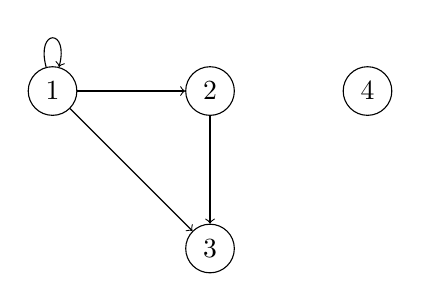
\begin{tikzpicture}[->,node distance=2cm]
  \node[draw,circle] (A) {$1$};
  \node[draw,circle] (B) [right of=A] {$2$};
  \node[draw,circle] (C) [below of=B] {$3$};
  \node[draw,circle] (D) [right of=B] {$4$};
  \draw (A) to [loop above]  (A);
  \draw (A) to  (B);
  \draw (A) to  (C);
  \draw (B) to  (C);
  \end{tikzpicture}
\intertext{এটি $V' = \{1, 2, 3\}$-বিশিষ্ট গ্রাফ $\tuple{V', E}$ থেকে আলাদা; সেই গ্রাফের চিত্র এইরকম:}
& 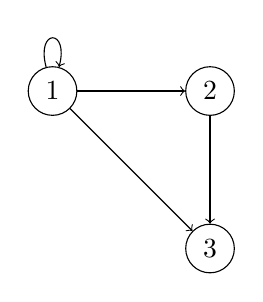
\begin{tikzpicture}[->,node distance=2cm]
  \node[draw,circle] (A) {$1$};
  \node[draw,circle] (B) [right of=A] {$2$};
  \node[draw,circle] (C) [below of=B] {$3$};
  \draw (A) to [loop above]  (A);
  \draw (A) to  (B);
  \draw (A) to  (C);
  \draw (B) to  (C);
  \end{tikzpicture}
\end{align*}
\end{ex}

\begin{prob}
  $\{1, 2, 3, 4\}$ সেটের উপর ছোট-অথবা-সমান সম্পর্ক~$\le$-কে গ্রাফ হিসেবে বিবেচনা করে তার চিত্র আঁকো।
\end{prob}

\end{document}
\end{filecontents*}

% content/sets-functions-relations/relations/operations.tex
\begin{filecontents*}[overwrite]{slc-module-130.tex}
% Part: sets-functions-relations
% Chapter: relations
% Section: operations

\documentclass[../../../include/open-logic-section]{subfiles}

\begin{document}

\olfileid[bn]{sfr}{rel}{ops}
\olsection{সম্পর্কের উপর ক্রিয়া}

প্রায়ই সম্পর্ক পরিবর্তন করা বা একাধিক সম্পর্ক একত্র করা কাজে আসে। \olref[sfr][rel][ord]{prop:stricttopartial}-এ আমরা সম্পর্কের \emph{সংযোগ} বিবেচনা করেছি; সম্পর্ক দুটিকে যুগলের সেট হিসেবে ধরলে এটি কেবল তাদের সেটসংযোগ। একইভাবে \olref[sfr][rel][ord]{prop:partialtostrict}-এ আমরা সম্পর্কের আপেক্ষিক অন্তর বিবেচনা করেছি। সম্পর্কের উপর করা যায় এমন আরও কয়েকটি ক্রিয়া এখানে দেওয়া হল।

\begin{defn}\ollabel{relationoperations}
ধরা যাক $R$, $S$ দুটি সম্পর্ক এবং $A$ যেকোনো সেট।

$R$-এর \emph{বিপরীত} হল $R^{-1} = \Setabs{\tuple{y, x}}{\tuple{x, y} \in R}$।

$R$ ও $S$-এর \emph{আপেক্ষিক গুণফল} হল $(R \mid S) = \{\tuple{x, z} : \exists y(Rxy \land Syz)\}$।

$R$-কে $A$-তে \emph{সীমাবদ্ধ} করলে পাওয়া যায় $\funrestrictionto{R}{A}= R \cap A^2$।

$A$-তে $R$-এর \emph{প্রয়োগ} হল $\funimage{R}{A} = \{y : (\exists x \in A)Rxy\}$
\end{defn}

\begin{ex}
ধরা যাক $S \subseteq \Int^2$ হল $\Int$-এর উপর উত্তরসূরি সম্পর্ক, অর্থাৎ $S = \Setabs{\tuple{x, y} \in \Int^2}{x + 1 = y}$; সুতরাং $Sxy$ যদি এবং কেবল যদি $x + 1 = y$।

$S^{-1}$ হল $\Int$-এর উপর পূর্বসূরি সম্পর্ক, অর্থাৎ $\Setabs{\tuple{x,y}\in\Int^2}{x -1 =y}$।

$S\mid S$ হল
$ \Setabs{\tuple{x,y}\in\Int^2}{x + 2 =y}$

$\funrestrictionto{S}{\Nat}$ হল $\Nat$-এর উপর উত্তরসূরি সম্পর্ক।

$\funimage{S}{\{1,2,3\}}$ হল $\{2, 3, 4\}$।
\end{ex}

\begin{defn}[পরিযায়ী আবরণ]ধরা যাক $R \subseteq A^2$ একটি দ্বিপদ সম্পর্ক।

$R$-এর \emph{পরিযায়ী আবরণ} হল $R^+ = \bigcup_{0 < n \in \Nat} R^n$, যেখানে আমরা পুনরাবৃত্তভাবে সংজ্ঞা দিই $R^1 = R$ এবং $R^{n+1} = R^n \mid R$।

$R$-এর \emph{প্রতিবিম্ব ও পরিযায়ী আবরণ} হল $R^* = R^+ \cup \Id{A}$।
\end{defn}

\begin{ex}
উত্তরসূরি সম্পর্ক $S \subseteq \Int^2$ নাও। $S^2xy$ যদি এবং কেবল যদি $x + 2 = y$, $S^3xy$ যদি এবং কেবল যদি $x + 3 = y$, ইত্যাদি। তাই $S^+xy$ যদি এবং কেবল যদি কোনো $n \geq 1$-এর জন্য $x + n = y$। অন্যভাবে বললে, $S^+xy$ যদি এবং কেবল যদি $x < y$, এবং $S^*xy$ যদি এবং কেবল যদি $x \le y$।
\end{ex}

\begin{prob}
দেখাও যে $R$-এর পরিযায়ী আবরণ সত্যিই পরিযায়ী।
\end{prob}

\end{document}
\end{filecontents*}

% content/sets-functions-relations/relations/orders.tex
\begin{filecontents*}[overwrite]{slc-module-131.tex}
% Part: sets-functions-relations
% Chapter: relations
% Section: orders

\documentclass[../../../include/open-logic-section]{subfiles}

\begin{document}

\olfileid[bn]{sfr}{rel}{ord}
\olsection{ক্রমসম্পর্ক}

\begin{explain}
আমাদের অনেক তুলনাতেই কিছু বস্তুকে কোনো বিশেষ দিক থেকে অন্য বস্তুর ``চেয়ে ছোট'', ``সমান'' বা ``চেয়ে বড়'' বলা হয়। এগুলি \emph{ক্রম}সম্পর্কের উদাহরণ। কিন্তু ক্রমসম্পর্কের নানা ধরন আছে। যেমন, কোনো কোনো ধরনের ক্ষেত্রে যেকোনো দুটি বস্তুকে তুলনা করা যায়, অন্যগুলির ক্ষেত্রে তা আবশ্যক নয়। কোনোটি অভিন্নতাকে অন্তর্ভুক্ত করে (যেমন~$\le$), আবার কোনোটি বাদ দেয় (যেমন~$<$)। তাই এখানে একটি শ্রেণিবিভাগ কাজে আসবে।
\end{explain}

\begin{defn}[প্রাক্‌ক্রম]
যে সম্পর্ক প্রতিবিম্ব ধর্মবিশিষ্ট এবং পরিযায়ী, তাকে \emph{প্রাক্‌ক্রম} বলা হয়।
\end{defn}

\begin{defn}[আংশিক ক্রম]
যে প্রাক্‌ক্রম বিপ্রতিসমও, তাকে \emph{আংশিক ক্রম} বলা হয়।
\end{defn}

\begin{defn}[রৈখিক ক্রম]\ollabel{def:linearorder}
যে আংশিক ক্রম সংযুক্তও, তাকে \emph{পূর্ণ ক্রম} বা \emph{রৈখিক ক্রম} বলা হয়।
\end{defn}

\begin{ex}
প্রত্যেক রৈখিক ক্রম আংশিক ক্রমও, এবং প্রত্যেক আংশিক ক্রম প্রাক্‌ক্রমও; কিন্তু বিপরীত দিকের দাবিগুলি সত্য নয়। $A$-এর উপর সার্বিক সম্পর্ক একটি প্রাক্‌ক্রম, কারণ তা প্রতিবিম্ব ধর্মবিশিষ্ট এবং পরিযায়ী। কিন্তু $A$-তে একটির বেশি !!{element} থাকলে সার্বিক সম্পর্ক বিপ্রতিসম নয়, তাই আংশিক ক্রমও নয়।
\end{ex}

\begin{ex}
$\Bin^*$-এর উপর \emph{চেয়ে দীর্ঘ নয়} সম্পর্ক $\preccurlyeq$ বিবেচনা করো: $x \preccurlyeq y$ যদি এবং কেবল যদি $\len{x} \le \len{y}$। এটি প্রাক্‌ক্রম (প্রতিবিম্ব ধর্মবিশিষ্ট এবং পরিযায়ী), এমনকি সংযুক্তও; কিন্তু আংশিক ক্রম নয়, কারণ এটি বিপ্রতিসম নয়। যেমন, $01 \preccurlyeq 10$ এবং $10 \preccurlyeq 01$, কিন্তু $01 \neq 10$।
\end{ex}

\begin{ex}
সেটের একটি সেটের উপর $\subseteq$ সম্পর্কটি একটি গুরুত্বপূর্ণ আংশিক ক্রম। সাধারণভাবে এটি রৈখিক ক্রম নয়; কারণ $a \neq b$ হলে $\Pow{\{a, b\}} = \{\emptyset, \{a\}, \{b\}, \{a,b\}\}$ বিবেচনা করে আমরা দেখি $\{a\} \nsubseteq \{b\}$ এবং $\{a\} \neq \{b\}$ এবং $\{b\} \nsubseteq \{a\}$।
\end{ex}

\begin{ex}
\emph{নিঃশেষে বিভাজ্যতার} সম্পর্ক থেকে আমরা এমন একটি আংশিক ক্রম পাই যা রৈখিক ক্রম নয়। পূর্ণসংখ্যা $n$ ও~$m$-এর জন্য $n \mid m$ লিখে আমরা বোঝাই যে $n$ দিয়ে $m$ নিঃশেষে বিভাজ্য, অর্থাৎ এমন একটি পূর্ণসংখ্যা~$k$ আছে যাতে $m = kn$ হয়। $\Nat$-এর উপর এটি আংশিক ক্রম, কিন্তু রৈখিক ক্রম নয়: যেমন, $2 \nmid 3$ এবং $3 \nmid 2$-ও। $\Int$-এর উপর সম্পর্ক হিসেবে বিবেচনা করলে বিভাজ্যতা কেবল প্রাক্‌ক্রম, কারণ তা বিপ্রতিসম নয়: $1 \mid -1$ এবং $-1 \mid 1$, কিন্তু $1 \neq -1$।
\end{ex}

\begin{ex}
অনুক্রমের সেট~$A^*$-এর উপর \emph{প্রসারণ} সম্পর্কটি এইরকম: $s \sqsubseteq s'$ যদি এবং কেবল যদি $s = \emptyseq$ (শূন্য অনুক্রম), $s = s'$, অথবা $s = \tuple{s_1, \dots, s_n}$ এবং $s' = \tuple{s_1, \dots, s_n, s_{n+1}, \dots, s_m}$ হয়। $s \sqsubseteq s'$ হলে আমরা $s$-কে $s'$-এর \emph{প্রারম্ভিক খণ্ড}ও বলি। $A^*$-এর উপর প্রসারণ সম্পর্ক আংশিক ক্রম, কিন্তু রৈখিক ক্রম নয়; যেমন, $a \neq b$ হলে $ab \not\sqsubseteq ba$ এবং $ba \not\sqsubseteq ab$।
\end{ex}

\begin{defn}[কঠোর ক্রম]
\emph{কঠোর ক্রম} হল এমন সম্পর্ক যা আত্মসম্পর্কহীন, একমুখী এবং পরিযায়ী।
\end{defn}

\begin{defn}[কঠোর রৈখিক ক্রম]\ollabel{def:strictlinearorder}
যে কঠোর ক্রম সংযুক্তও, তাকে \emph{কঠোর পূর্ণ ক্রম} বা \emph{কঠোর রৈখিক ক্রম} বলা হয়।
\end{defn}

\begin{ex}
$\le$ হল কঠোর রৈখিক ক্রম~$<$-এর অনুরূপ রৈখিক ক্রম। $\subseteq$ হল কঠোর ক্রম~$\subsetneq$-এর অনুরূপ আংশিক ক্রম।
\end{ex}

$A$-এর উপর যেকোনো কঠোর ক্রম $R$-কে কর্ণ $\Id{A}$ যোগ করে, অর্থাৎ সব~$\tuple{x, x}$ যুগল যোগ করে, আংশিক ক্রমে রূপান্তরিত করা যায়। (একে $R$-এর \emph{প্রতিবিম্ব আবরণ} বলা হয়।) বিপরীতভাবে, একটি আংশিক ক্রম থেকে শুরু করে $\Id{A}$ বাদ দিলে কঠোর ক্রম পাওয়া যায়। পরের দুটি ফল এই কথাগুলিই সুনির্দিষ্টভাবে প্রকাশ করে।

\begin{prop}\ollabel{prop:stricttopartial}
যদি $R$, $A$-এর উপর কঠোর ক্রম হয়, তবে $R^+ = R \cup \Id{A}$ আংশিক ক্রম। আরও, $R$ কঠোর রৈখিক ক্রম হলে $R^+$ রৈখিক ক্রম।
\end{prop}

\begin{proof}
ধরা যাক, $R$ কঠোর ক্রম; অর্থাৎ $R \subseteq A^2$ এবং $R$ আত্মসম্পর্কহীন, একমুখী ও পরিযায়ী। ধরি $R^+ = R \cup \Id{A}$। আমাদের দেখাতে হবে যে $R^+$ প্রতিবিম্ব ধর্মবিশিষ্ট, বিপ্রতিসম এবং পরিযায়ী।

$R^+$ যে প্রতিবিম্ব ধর্মবিশিষ্ট তা স্পষ্ট, কারণ সকল $x \in A$-এর জন্য $\tuple{x, x} \in \Id{A} \subseteq R^+$।

$R^+$ বিপ্রতিসম দেখাতে স্ববিরোধে পৌঁছানোর উদ্দেশ্যে ধরা যাক $R^+xy$ এবং $R^+yx$, কিন্তু $x \neq y$। যেহেতু $\tuple{x,y} \in R \cup \Id{A}$, অথচ $\tuple{x, y} \notin \Id{A}$, তাই অবশ্যই $\tuple{x, y} \in R$, অর্থাৎ $Rxy$। একইভাবে,~$Ryx$। কিন্তু এটি $R$ একমুখী হওয়ার অনুমানের বিরোধী।

পরিযায়িতা প্রতিষ্ঠা করতে ধরা যাক $R^+xy$ এবং $R^+yz$। যদি $\tuple{x, y} \in R$ এবং $\tuple{y,z} \in R$ উভয়ই হয়, তবে $R$~পরিযায়ী বলে $\tuple{x, z} \in R$। অন্যথায়, হয় $\tuple{x, y} \in \Id{A}$, অর্থাৎ $x = y$, নয়তো $\tuple{y, z} \in \Id{A}$, অর্থাৎ $y = z$। প্রথম ক্ষেত্রে অনুমান অনুসারে $R^+yz$, এবং $x = y$; তাই $R^+xz$। দ্বিতীয় ক্ষেত্রেও একইরকম। উভয় ক্ষেত্রেই $R^+xz$; সুতরাং $R^+$-ও পরিযায়ী।

``আরও'' অংশটির জন্য ধরা যাক $R$ সংযুক্তও। তাহলে সকল $x \neq y$-এর জন্য হয় $Rxy$, নয়তো~$Ryx$; অর্থাৎ হয় $\tuple{x, y} \in R$, নয়তো $\tuple{y, x} \in R$। যেহেতু $R \subseteq R^+$, তাই $R^+$-এর ক্ষেত্রেও এটি সত্য থাকে; সুতরাং $R^+$-ও সংযুক্ত।
\end{proof}

\begin{prop}\ollabel{prop:partialtostrict}
যদি $R$, $A$-এর উপর আংশিক ক্রম হয়, তবে $R^- = R \setminus \Id{A}$ কঠোর ক্রম। আরও, $R$ রৈখিক ক্রম হলে $R^-$ কঠোর রৈখিক ক্রম।
\end{prop}

\begin{proof}
এটি অনুশীলন হিসেবে রাখা হল।
\end{proof}

\begin{prob}
\olref[sfr][rel][ord]{prop:partialtostrict}-এর একটি প্রমাণ দাও।
\end{prob}

পরের সহজ ফলটি প্রতিষ্ঠা করে যে কঠোর রৈখিক ক্রম সদস্যভিত্তিক সমতার নীতির অনুরূপ একটি ধর্ম মেনে চলে:

\begin{prop}\ollabel{prop:extensionality-strictlinearorders}
যদি $<$, $A$-এর উপর কঠোর রৈখিক ক্রম হয়, তবে:
\[
  (\forall a, b \in A)((\forall x \in A)(x < a \liff x < b) \lif a = b).
\]
\end{prop}

\begin{proof}
ধরা যাক $(\forall x \in A)(x < a \liff x < b)$। যদি $a < b$ হয়, তবে $a < a$ হয়, যা $<$ আত্মসম্পর্কহীন হওয়ার বিরোধী; তাই $a \nless b$। ঠিক একইভাবে $b \nless a$। সুতরাং $a = b$, কারণ $<$ সংযুক্ত।
\end{proof}

\end{document}
\end{filecontents*}

% content/sets-functions-relations/relations/relations-as-sets.tex
\begin{filecontents*}[overwrite]{slc-module-132.tex}
% Part: sets-functions-relations
% Chapter: relations
% Section: relations-as-sets

\documentclass[../../../include/open-logic-section]{subfiles}

\begin{document}

\olfileid[bn]{sfr}{rel}{set}
\olsection{সেট হিসেবে সম্পর্ক}

\begin{explain}
\olref[sfr][set][imp]{sec}-এ কয়েকটি গুরুত্বপূর্ণ সেটের কথা বলেছি:
$\Nat$, $\Int$, $\Rat$, $\Real$। এই সেটগুলির কোনও কোনওটির
!!{element}sের মধ্যে কিছু আকর্ষণীয় সম্পর্ক তোমার নিশ্চয়ই মনে আছে।
যেমন, প্রতিটি সেটেই একটি সুপরিচিত \emph{ক্রমসম্পর্ক} আছে।
এ ছাড়াও আছে \emph{অভিন্ন হওয়ার} সম্পর্ক: প্রতিটি বস্তু নিজের সঙ্গে
এই সম্পর্কে থাকে, অন্য কোনও বস্তুর সঙ্গে নয়। আরও অনেক আকর্ষণীয়
সম্পর্কের সঙ্গে আমাদের পরিচয় হবে; সম্ভাব্য সম্পর্কের সংখ্যা আরও বেশি।
তবে সেগুলির আলোচনা করার আগে দেখাব যে, সম্পর্ককে বিশেষ ধরনের
সেট হিসেবে দেখা যায়।

এর জন্য \olref[sfr][set][pai]{sec}-এর দুটি বিষয় মনে করো। প্রথমটি
\emph{ক্রমযুগলের} ধারণা: $a$ ও $b$ দেওয়া থাকলে $\tuple{a, b}$
গঠন করতে পারি। এখানে উপাদানের ক্রম \emph{অবশ্যই} গুরুত্বপূর্ণ।
তাই $a \neq b$ হলে $\tuple{a, b} \neq \tuple{b, a}$।
(ক্রমহীন যুগল, অর্থাৎ $2$-উপাদানবিশিষ্ট সেটের সঙ্গে তুলনা করো;
সেখানে $\{a, b\}=\{b, a\}$।) দ্বিতীয়টি \emph{কার্তেসীয় গুণফলের}
ধারণা: $A$ ও $B$ সেট হলে $A \times B$ গঠন করতে পারি।
এটি $x \in A$ এবং $y \in B$ এমন সমস্ত যুগল $\tuple{x, y}$-এর সেট।
বিশেষত, $A^{2}= A \times A$ হল $A$ থেকে গঠিত সমস্ত ক্রমযুগলের সেট।

এবার কোনও সেটের উপর একটি নির্দিষ্ট সম্পর্ক বিবেচনা করব:
স্বাভাবিক সংখ্যার সেট~$\Nat$-এর উপর $<$-সম্পর্ক। সংখ্যার সেই সমস্ত
যুগল $\tuple{n, m}$-এর সেট বিবেচনা করো, যাদের জন্য $n<m$। অর্থাৎ,
\[
  R=\Setabs{\tuple{n, m}}{n, m \in \Nat \text{ এবং } n<m}.
\]
$n$, $m$-এর চেয়ে ছোট হওয়া এবং $\tuple{n, m}$ যুগলটি $R$-এর সদস্য
হওয়ার মধ্যে ঘনিষ্ঠ যোগ আছে:
\[
      n<m\text{ হবে যদি এবং কেবল যদি }\tuple{n, m} \in R.
\]
বস্তুত, কোনও তথ্য না হারিয়েই $R$ সেটটিকে $\Nat$-এর উপর
$<$-সম্পর্ক \emph{হিসেবেই} বিবেচনা করতে পারি।

একইভাবে, সংখ্যার মধ্যে যে-কোনও সম্পর্কের জন্য $\Nat^{2}$-এর
একটি উপসেট গঠন করতে পারি। বিপরীতভাবে, সংখ্যার যুগলের যে-কোনও সেট
$S \subseteq \Nat^{2}$ দেওয়া থাকলে, সংখ্যার মধ্যে তার অনুরূপ একটি
সম্পর্ক থাকে: $n$, $m$-এর সঙ্গে সেই সম্পর্কে থাকবে যদি এবং কেবল যদি
$\tuple{n, m} \in S$ হয়। এর ভিত্তিতে নিচের সংজ্ঞা দিচ্ছি:
\end{explain}

\begin{defn}[দ্বিপদ সম্পর্ক]
কোনও সেট $A$-এর উপর \emph{দ্বিপদ সম্পর্ক} হল $A^{2}$-এর একটি উপসেট।
$R \subseteq A^{2}$ যদি $A$-এর উপর দ্বিপদ সম্পর্ক হয় এবং
$x, y \in A$ হয়, তবে $\tuple{x, y} \in R$ বোঝাতে কখনও
$Rxy$ (অথবা $xRy$) লিখি।
\end{defn}

\begin{ex}
  \ollabel{relations}
স্বাভাবিক সংখ্যার যুগলগুলির সেট $\Nat^{2}$-কে নিচের মতো
দ্বিমাত্রিক ম্যাট্রিক্সে সাজানো যায়:
\[
  \begin{array}{ccccc}
  \mathbf{\tuple{ 0,0 }} & \tuple{ 0,1 } &
    \tuple{ 0,2 } & \tuple{ 0,3 } & \ldots\\
  \tuple{ 1,0 } & \mathbf{\tuple{ 1,1 }} &
    \tuple{ 1,2 } & \tuple{ 1,3 } & \ldots\\
  \tuple{ 2,0 } & \tuple{ 2,1 } &
    \mathbf{\tuple{ 2,2 }} & \tuple{ 2,3 } & \ldots\\
  \tuple{ 3,0 } & \tuple{ 3,1 } & \tuple{ 3,2 } &
    \mathbf{\tuple{ 3,3 }} & \ldots\\
  \vdots & \vdots & \vdots & \vdots & \mathbf{\ddots}
  \end{array}
\]
এখানে কর্ণের যুগলগুলি মোটা হরফে দেখিয়েছি। কারণ, কর্ণের যুগলগুলি
নিয়ে গঠিত $\Nat^2$-এর উপসেটটি, অর্থাৎ
\[
  \{\tuple{0,0 }, \tuple{ 1,1 }, \tuple{ 2,2 }, \dots\},
  \]
হল \emph{$\Nat$-এর উপর অভিন্নতার সম্পর্ক}। (এই সম্পর্কটি বহুল
ব্যবহৃত বলে, যে-কোনও সেট $A$-এর জন্য
$\Id{A}=\Setabs{\tuple{ x,x }}{x \in A}$ সংজ্ঞায়িত করি।)
কর্ণের উপরের সমস্ত যুগলের উপসেটটি, অর্থাৎ
\[
  L = \{\tuple{ 0,1 },\tuple{ 0,2 },\ldots,\tuple{ 1,2 },
  \tuple{ 1,3 }, \dots, \tuple{ 2,3 }, \tuple{ 2,4 },\ldots\},
\]
হল \emph{চেয়ে ছোট হওয়ার} সম্পর্ক: $Lnm$ হবে যদি এবং কেবল যদি
$n<m$ হয়। কর্ণের নিচের যুগলগুলির উপসেটটি, অর্থাৎ
\[
  G=\{ \tuple{ 1,0 },\tuple{ 2,0 },\tuple{
    2,1 }, \tuple{ 3,0 },\tuple{ 3,1 },\tuple{ 3,2 }, \dots\},
\]
হল \emph{চেয়ে বড় হওয়ার} সম্পর্ক: $Gnm$ হবে যদি এবং কেবল যদি
$n>m$ হয়। $L$ ও $I$-এর সংযোগকে $K=L\cup I$ বললে, সেটি
\emph{চেয়ে ছোট বা সমান হওয়ার} সম্পর্ক: $Knm$ হবে যদি এবং কেবল যদি
$n \le m$ হয়। একইভাবে, $H=G \cup I$ হল \emph{চেয়ে বড় বা সমান
হওয়ার সম্পর্ক}। এই $L$, $G$, $K$ ও $H$ বিশেষ ধরনের সম্পর্ক,
যাদের \emph{ক্রম} বলে। $L$ ও $G$-এর একটি ধর্ম হল: কোনও সংখ্যাই
নিজের সঙ্গে $L$ বা $G$ সম্পর্কে থাকে না (অর্থাৎ, সমস্ত $n$-এর জন্য,
$Lnn$ কিংবা $Gnn$, কোনওটিই হয় না)। এই ধর্মবিশিষ্ট সম্পর্ককে
\emph{আত্মসম্পর্কহীন} বলে। সেটি একই সঙ্গে ক্রম হলে তাকে
\emph{কঠোর ক্রম} বলা হয়।
\end{ex}

\begin{explain}
ক্রম ও অভিন্নতা গুরুত্বপূর্ণ এবং স্বাভাবিক সম্পর্ক হলেও জোর দিয়ে বলা
দরকার যে, আমাদের সংজ্ঞা অনুযায়ী $A^{2}$-এর \emph{যে-কোনও} উপসেটই
$A$-এর উপর সম্পর্ক, সেটিকে যতই অস্বাভাবিক বা কৃত্রিম মনে হোক।
বিশেষত, $\emptyset$ যে-কোনও সেটের উপর সম্পর্ক। একে \emph{শূন্য
সম্পর্ক} বলে; কোনও উপাদানযুগলই এই সম্পর্কে থাকে না। আবার $A^{2}$
নিজেও $A$-এর উপর সম্পর্ক: প্রতিটি যুগলই এই সম্পর্কে থাকে।
একে \emph{সার্বিক সম্পর্ক} বলে। তবে
$E=\Setabs{\tuple{n, m}}{n>5 \text{ অথবা } m \times n \ge 34}$-এর
মতো কিছুও সম্পর্ক হিসেবে গণ্য হয়।
\end{explain}

\begin{prob}
  $\Pow{\{a, b, c\}}$ সেটের উপর $\subseteq$ সম্পর্কটির
  !!{element}sের তালিকা তৈরি করো।
\end{prob}

\end{document}
\end{filecontents*}

% content/sets-functions-relations/relations/relations.tex
\begin{filecontents*}[overwrite]{slc-module-133.tex}
% Part: sets-functions-relations
% Chapter: relations

\documentclass[../../../include/open-logic-chapter]{subfiles}

\begin{document}

\olchapter{sfr}{rel}{সম্পর্ক}

\slcEmbeddedImport{slc-module-132.tex}

\slcEmbeddedImport{slc-module-134.tex}

\slcEmbeddedImport{slc-module-128.tex}

\slcEmbeddedImport{slc-module-131.tex}

\slcEmbeddedImport{slc-module-129.tex}

\slcEmbeddedImport{slc-module-135.tex}

\slcEmbeddedImport{slc-module-130.tex}

\OLEndChapterHook

\end{document}
\end{filecontents*}

% content/sets-functions-relations/relations/special-properties.tex
\begin{filecontents*}[overwrite]{slc-module-134.tex}
% Part: sets-functions-relations
% Chapter: relations
% Section: special-properties

\documentclass[../../../include/open-logic-section]{subfiles}

\begin{document}

\olfileid[bn]{sfr}{rel}{prp}
\olsection{সম্পর্কের বিশেষ ধর্ম}

\begin{intro}
কয়েক ধরনের সম্পর্ক এত ঘন ঘন দেখা যায় যে তাদের বিশেষ নাম দেওয়া হয়েছে। যেমন, $\le$ এবং~$\subseteq$ নিজ নিজ ক্ষেত্রের (ধরা যাক, $\le$-এর ক্ষেত্রে $\Nat$ এবং $\subseteq$-এর ক্ষেত্রে $\Pow{A}$) মধ্যে একই ধরনের সম্পর্ক স্থাপন করে। এই সম্পর্কগুলির মিল ও অমিল ঠিক কোথায়, তা বোঝার জন্য আমরা সম্পর্কের কয়েকটি বিশেষ ধর্ম অনুসারে তাদের শ্রেণিবদ্ধ করি। দেখা যায়, এই ধর্মগুলির কয়েকটির সমন্বয় বিশেষ গুরুত্বপূর্ণ: ক্রমসম্পর্ক এবং তুল্যতা সম্পর্ক।
\end{intro}

\begin{defn}[প্রতিবিম্ব ধর্ম]
একটি সম্পর্ক $R \subseteq A^2$ \emph{প্রতিবিম্ব ধর্মবিশিষ্ট} যদি এবং কেবল যদি প্রত্যেক $x \in A$-এর জন্য $Rxx$ হয়।
\end{defn}

\begin{defn}[পরিযায়িতা]
একটি সম্পর্ক $R \subseteq A^2$ \emph{পরিযায়ী} যদি এবং কেবল যদি যখনই $Rxy$ এবং $Ryz$ হয়, তখনই $Rxz$-ও হয়।
\end{defn}

\begin{defn}[প্রতিসাম্য]
একটি সম্পর্ক~$R \subseteq A^2$ \emph{প্রতিসম} যদি এবং কেবল যদি যখনই $Rxy$ হয়, তখনই~$Ryx$-ও হয়।
\end{defn}

\begin{defn}[বিপ্রতিসাম্য]
একটি সম্পর্ক~$R \subseteq A^2$ \emph{বিপ্রতিসম} যদি এবং কেবল যদি $Rxy$ ও $Ryx$ উভয়ই হলে $x=y$ হয় (অন্যভাবে বললে: $x\neq y$ হলে হয় $\lnot Rxy$, নয়তো $\lnot Ryx$)।
\end{defn}

\begin{explain}
প্রতিসম সম্পর্কে $Rxy$ ও $Ryx$ সর্বদা একসঙ্গে সত্য হয়, অথবা কোনোটিই সত্য হয় না। বিপ্রতিসম সম্পর্কে $Rxy$ ও $Ryx$ একসঙ্গে সত্য হওয়ার একমাত্র সম্ভাবনা হল $x = y$। লক্ষ করো, এর অর্থ এই নয় যে $x = y$ হলে $Rxy$ ও $Ryx$ \emph{অবশ্যই} সত্য হবে; কেবল এটুকুই যে তা নিষিদ্ধ নয়। তাই বিপ্রতিসম সম্পর্ক প্রতিবিম্ব ধর্মবিশিষ্ট হতে পারে, কিন্তু প্রত্যেক বিপ্রতিসম সম্পর্ক প্রতিবিম্ব ধর্মবিশিষ্ট নয়। আরও লক্ষ করো, বিপ্রতিসম হওয়া এবং কেবল প্রতিসম না হওয়া ভিন্ন শর্ত। বস্তুত, একটি সম্পর্ক একই সঙ্গে প্রতিসম ও বিপ্রতিসম হতে পারে (যেমন, অভিন্নতার সম্পর্ক)।
\end{explain}

\begin{defn}[সংযুক্ততা]
একটি সম্পর্ক $R \subseteq A^2$ \emph{সংযুক্ত} যদি সকল $x,y\in A$-এর জন্য, $x \neq y$ হলে হয় $Rxy$, নয়তো~$Ryx$ হয়।
\end{defn}

\begin{prob}
এমন সম্পর্কের উদাহরণ দাও যা (a) প্রতিবিম্ব ধর্মবিশিষ্ট ও প্রতিসম কিন্তু পরিযায়ী নয়, (b) প্রতিবিম্ব ধর্মবিশিষ্ট ও বিপ্রতিসম, (c) বিপ্রতিসম ও পরিযায়ী কিন্তু প্রতিবিম্ব ধর্মবিশিষ্ট নয়, এবং (d) প্রতিবিম্ব ধর্মবিশিষ্ট, প্রতিসম ও পরিযায়ী। সংখ্যা বা সেটের উপর সম্পর্ক ব্যবহার কোরো না।
\end{prob}

\begin{defn}[আত্মসম্পর্কহীনতা]
একটি সম্পর্ক $R \subseteq A^2$-কে \emph{আত্মসম্পর্কহীন} বলা হয় যদি সকল $x \in A$-এর জন্য $Rxx$ সত্য না হয়।
\end{defn}

\begin{defn}[একমুখিতা]
একটি সম্পর্ক $R \subseteq A^2$-কে \emph{একমুখী} বলা হয় যদি কোনো $x,y\in A$ যুগলের জন্যই $Rxy$ ও~$Ryx$ একসঙ্গে সত্য না হয়।
\end{defn}

লক্ষ করো, $A \neq \emptyset$ হলে $A$-এর উপর কোনো আত্মসম্পর্কহীন সম্পর্ক প্রতিবিম্ব ধর্মবিশিষ্ট হয় না, এবং $A$-এর উপর প্রত্যেক একমুখী সম্পর্ক বিপ্রতিসমও হয়। কিন্তু এমন $R \subseteq A^2$ আছে যা প্রতিবিম্ব ধর্মবিশিষ্টও নয়, আত্মসম্পর্কহীনও নয়; আবার এমন বিপ্রতিসম সম্পর্ক আছে যা একমুখী নয়।

\end{document}
\end{filecontents*}

% content/sets-functions-relations/relations/trees.tex
\begin{filecontents*}[overwrite]{slc-module-135.tex}
% Part: sets-functions-relations
% Chapter: relations
% Section: trees

\documentclass[../../../include/open-logic-section]{subfiles}

\begin{document}

\olfileid[bn]{sfr}{rel}{tre}
\olsection{বৃক্ষ}

একটি বিশেষ ধরনের আংশিক ক্রম, যা যুক্তিবিদ্যার সব শাখায় গুরুত্বপূর্ণ ভূমিকা পালন করে, হল \emph{বৃক্ষ}। যুক্তিবিদ্যার প্রাথমিক অংশে সসীম বৃক্ষ দেখা যায়: যেমন, !!{formula}sকে তাদের গঠন অনুসারে একটি বাক্যতাত্ত্বিক বৃক্ষে ভেঙে বোঝা যায়, আবার বহু !!{derivation} পদ্ধতিতে !!{derivation}sও সসীম বৃক্ষের আকার নেয়।
%
বচনমূলক এবং প্রথম-ক্রমের যুক্তিবিদ্যার পূর্ণতা উপপাদ্যের প্রমাণেই অসীম বৃক্ষের ব্যবহার দেখা যায়, এবং গাণিতিক যুক্তিবিদ্যার সর্বত্র এগুলি ব্যবহৃত হয়।

বৃক্ষের সেটতাত্ত্বিক ধারণাটি গ্রাফতত্ত্বের বৃক্ষ ধারণার ঘনিষ্ঠ। এখানে একটি (সসীম) বৃক্ষের ছবি দেওয়া হল:

\begin{center}
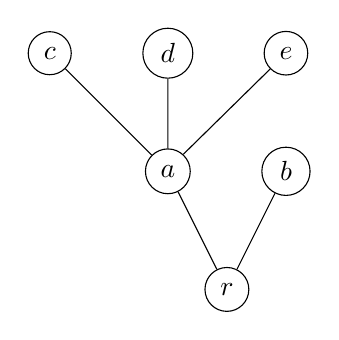
\begin{tikzpicture}[nodes={draw, circle}, -]
\node{$r$} [grow'=up]
    child { node {$a$}
        child { node {$c$} }
        child { node {$d$} }
        child { node {$e$} }
    }
    child { node {$b$} };
\end{tikzpicture}
\end{center}

সবচেয়ে নীচের নোড~$r$ হল মূল। $r$ ছাড়া প্রত্যেক নোডের ঠিক নীচে একটি মাত্র জনক নোড আছে। নোড~$x$ এবং নোড~$y$-এর মধ্যে এই সম্পর্কটি বিবেচনা করো: প্রান্ত বরাবর উপরের দিকে গিয়ে $x$ থেকে $y$-তে পৌঁছানো যায়। এই সম্পর্ককে $x$-এর $y$-এর \emph{পূর্বপুরুষ} হওয়া হিসেবে ভাবতে পারি।

বৃক্ষের পূর্বপুরুষ সম্পর্ক একটি কঠোর আংশিক ক্রম। এখান থেকেই সেটতাত্ত্বিক সংজ্ঞার প্রেরণা আসে। সংজ্ঞাটি দিতে আমাদের দুটি ধারণা দরকার। $\le$ দ্বারা আংশিকভাবে ক্রমিত সেট~$A$-এর একটি \emph{ক্ষুদ্রতম উপাদান} হল এমন !!a{element} $x \in A$, যার জন্য সকল $y \in A$-এর ক্ষেত্রে~$x \le y$ হয়। একটি সেট $\le$ দ্বারা \emph{সুক্রমিত} যদি তার প্রত্যেক অশূন্য উপসেটের ক্ষুদ্রতম উপাদান থাকে।

\begin{defn}[বৃক্ষ]
একটি \emph{বৃক্ষ} হল যুগল $T = \tuple{A, \le}$, যেখানে $A$ একটি সেট এবং $\le$, $A$-এর উপর আংশিক ক্রম; এর একটি অনন্য ক্ষুদ্রতম উপাদান $r \in A$ আছে (যাকে \emph{মূল} বলা হয়), এবং সকল $x \in A$-এর জন্য $\Setabs{y}{y \le x}$ সেটটি $\le$ দ্বারা সুক্রমিত।
\end{defn}

\begin{defn}[উত্তরসূরি]
ধরা যাক, $T = \tuple{A, \le}$ একটি বৃক্ষ। যদি $x,y \in A$, $x < y$, এবং এমন কোনো $z \in A$ না থাকে যাতে $x < z < y$ হয়, তবে আমরা $y$-কে $x$-এর \emph{উত্তরসূরি} বলি।
\end{defn}

$x \in A$-এর উত্তরসূরিদের তার \emph{সন্তান}ও বলা হয়। যদি $y$, $x$-এর উত্তরসূরি হয়, তবে $x$-কে $y$-এর \emph{পূর্বসূরি} বা \emph{জনক} বলি।

\begin{prop}
যদি $\tuple{A,\le}$ একটি বৃক্ষ হয়, তবে মূল ছাড়া প্রত্যেক $x \in A$-এর সর্বাধিক একজন পূর্বসূরি থাকে।
\end{prop}

\begin{proof}
  ধরা যাক $y_1 < x$ এবং $y_2 < x$ এবং $y_1 \neq y_2$। তাহলে $\{y_1, y_2\} \subseteq \Setabs{z}{z<x}$। যেহেতু $\Setabs{z}{z<x}$, $\le$ দ্বারা সুক্রমিত, তাই তার উপসেট $\{y_1, y_2\}$-এর ক্ষুদ্রতম উপাদান আছে, যা অবশ্যই হয় $y_1$, নয়তো~$y_2$। তাই হয় $y_1 \le y_2$, নয়তো $y_2 \le y_1$। আমরা $y_1 \neq y_2$ ধরে নিয়েছিলাম; তাই আসলে হয় $y_1 < y_2$, নয়তো $y_2 < y_1$। আবার যেহেতু আমরা $y_1 < x$ এবং $y_2 < x$ ধরে নিয়েছিলাম, তাই আরও পাই, হয় $y_1 < y_2 < x$, নয়তো $y_2 < y_1 < x$। সুতরাং $y_1$ ও $y_2$ উভয়েই $x$-এর পূর্বসূরি হতে পারে না।
\end{proof}

\begin{defn}
একটি বৃক্ষ $T = \tuple{A, \le}$-কে \emph{অসীম} বলা হয় যদি $A$ অসীম সেট হয়; অন্যথায় তাকে \emph{সসীম} বলা হয়। যদি $T$-তে প্রত্যেক $x \in A$-এর কেবল সসীমসংখ্যক উত্তরসূরি থাকে, তবে আমরা $T$-কে \emph{সসীম শাখায়িত} বলি।
\end{defn}

\begin{defn}[শাখা]
একটি বৃক্ষ $T = \tuple{A, \le}$ দেওয়া থাকলে, $T$-এর একটি \emph{শাখা} হল $T$-এর একটি অন্তর্ভুক্তির বিচারে সর্বাধিক শৃঙ্খল; অর্থাৎ এমন সেট $B \subseteq A$ যাতে যেকোনো $x, y \in B$-এর জন্য হয় $x \le y$, নয়তো $y \le x$, এবং যেকোনো $z \in X \setminus B$-এর জন্য এমন $u \in B$ আছে যাতে $z \le u$ বা $u \le z$ কোনোটিই হয় না।
%
$T$-এর সব শাখার সেট বোঝাতে আমরা $[T]$ ব্যবহার করি।
\end{defn}

\begin{ex}
সসীম শাখায়িত বৃক্ষের একটি পরিচিত উদাহরণ হল $0$ ও~$1$-এর সসীম অনুক্রমগুলি নিয়ে গঠিত \emph{অসীম দ্বিমিক বৃক্ষ}, যাকে কখনো কখনো $\{0,1\}^*$ বা~$\Bin^*$ দিয়ে বোঝানো হয় এবং প্রসারণ সম্পর্ক $\sqsubseteq$ দ্বারা ক্রমিত করা হয় (যেমন, $101 \sqsubseteq 101101$)। যেহেতু যেকোনো দ্বিমিক প্রতীকক্রমের শেষে একটি $0$ বা একটি $1$ যোগ করে তাকে সর্বদা বাড়ানো যায়, তাই এই বৃক্ষে অসীমসংখ্যক উপাদান আছে: প্রত্যেক উপাদান~$s$-এর ঠিক দুটি উত্তরসূরি আছে, $s0$ এবং~$s1$। এর মূল হল শূন্য অনুক্রম $\emptyseq$।
\end{ex}

\begin{ex}
আরও একটু সাধারণভাবে, স্বাভাবিক সংখ্যার সসীম অনুক্রমের সেট~$\Nat^*$-ও প্রসারণ সম্পর্ক~$\sqsubseteq$ সমেত একটি বৃক্ষ। এটি যে সসীম শাখায়িত নয় তা স্পষ্ট: প্রত্যেক $s \in \Nat^*$-এর অসীমসংখ্যক উত্তরসূরি~$sn$ আছে, প্রত্যেক $n \in \Nat$-এর জন্য একটি করে। $\sqsubseteq$-এর অধীনে বদ্ধ প্রত্যেক $A \subseteq \Nat^*$ হল $\Nat^*$-এর একটি \emph{উপবৃক্ষ}। (অর্থাৎ $A$ এমন যে $s \in A$ এবং $s' \sqsubseteq s$ হলে $s' \in A$-ও হয়।) সব সসীম বৃক্ষকে $\Nat^*$-এর সসীম উপবৃক্ষ হিসেবে প্রকাশ করা যায়।
\end{ex}

\begin{prop}[ক্যোনিগের সহায়ক উপপাদ্য]
যদি $T = \tuple{A,\le}$ একটি সসীম শাখায়িত অসীম বৃক্ষ হয়, তবে $T$-এর একটি অসীম শাখা আছে।
\end{prop}

গণনাযোগ্যতা তত্ত্বে বহুল ব্যবহৃত ক্যোনিগের সহায়ক উপপাদ্যের একটি বিশেষ ক্ষেত্র, যাকে \emph{দুর্বল ক্যোনিগের সহায়ক উপপাদ্য} বলা হয়, হল: $\{0,1\}^*$-এর যেকোনো অসীম উপবৃক্ষের একটি অসীম শাখা আছে।

\end{document}
\end{filecontents*}

% content/sets-functions-relations/sets-functions-relations.tex
\begin{filecontents*}[overwrite]{slc-module-136.tex}
% Part: Sets, Relations, Functions

\documentclass[../../include/open-logic-part]{subfiles}

\begin{document}

\olpart{sfr}{সেট, সম্পর্ক, অপেক্ষক}


\slcEmbeddedImport{slc-module-141.tex}

\slcEmbeddedImport{slc-module-133.tex}

\slcEmbeddedImport{slc-module-125.tex}

\slcEmbeddedImport{slc-module-153.tex}

\OLEndPartHook
\end{document}
\end{filecontents*}

% content/sets-functions-relations/sets/basics.tex
\begin{filecontents*}[overwrite]{slc-module-137.tex}
% Part: sets-functions-relations
% Chapter: sets
% Section: basics

\documentclass[../../../include/open-logic-section]{subfiles}

\begin{document}

\olfileid[bn]{sfr}{set}{bas}
\olsection{সদস্যভিত্তিক সমতার নীতি}

কতগুলি বস্তুর সমষ্টিকে {একটি} বস্তু হিসেবে বিবেচনা করলে তাকে \emph{সেট} বলে।
যে বস্তুগুলি নিয়ে সেটটি গঠিত, সেগুলিকে সেটটির \emph{উপাদান} বা
\emph{সদস্য} বলা হয়। $x$ যদি কোনও সেট~$A$-এর !!a{element} হয়, তবে আমরা
$x \in A$ লিখি; তা না হলে $x \notin A$ লিখি। যে সেটের কোনও
!!{element}s নেই, তাকে \emph{শূন্য} সেট বলে এবং
``$\emptyset$'' দিয়ে নির্দেশ করা হয়।

\begin{explain}
আমরা সেটটি কীভাবে \emph{নির্দেশ} করি, তার !!{element}s কী \emph{ক্রমে}
সাজাই, কিংবা তার !!{element}s \emph{কত বার} গুনি, তা বিবেচ্য নয়।
বিবেচ্য কেবল এই যে, তার !!{element}s কী কী। নিচের নীতিতে আমরা
এই কথাটিই সুনির্দিষ্টভাবে প্রকাশ করি।
\end{explain}

\begin{defn}[সদস্যভিত্তিক সমতার নীতি]
  $A$ ও $B$ সেট হলে, $A = B$ হবে যদি এবং কেবল যদি
  $A$-এর প্রতিটি !!{element} $B$-এরও !!a{element} হয় এবং
  বিপরীত দিক থেকেও একই কথা সত্য হয়।
\end{defn}

সদস্যভিত্তিক সমতার নীতি কিছু প্রতীক ব্যবহারের ভিত্তি দেয়। সাধারণভাবে,
কতগুলি বস্তু $a_{1}$, \dots, $a_{n}$ দেওয়া থাকলে,
$\{a_{1}, \dots, a_{n}\}$ হল \emph{সেই নির্দিষ্ট} সেট, যার
!!{element}s হল $a_1, \ldots, a_n$। এখানে ``\emph{সেই নির্দিষ্ট}''
কথাটির উপর জোর দিচ্ছি, কারণ সদস্যভিত্তিক সমতার নীতি অনুযায়ী এমন সেট
\emph{একটিই} হতে পারে। এই নীতি নিচের সমতাও সমর্থন করে:
  \[
    \{a, a, b\} = \{a, b\} = \{b,a\}.
  \]
এতে আগের কথাটিই স্পষ্ট হয়: সেট বিবেচনার সময় তার !!{element}sের
ক্রম কিংবা সেগুলি কত বার উল্লেখ করা হয়েছে, তা নিয়ে আমাদের মাথা ঘামাতে হয় না।

\begin{tagblock}{novice}
\begin{ex}
কতগুলি বস্তু দেওয়া থাকলে, সেগুলিকে একত্র করে একটি সেট গঠন করা যায়।
যেমন, রিচার্ডের ভাইবোনদের সেটে একজন ব্যক্তি আছেন; সেটটিকে আমরা
$S=\{\textrm{রুথ}\}$ লিখতে পারি। $4$-এর চেয়ে ছোট ধনাত্মক পূর্ণসংখ্যাগুলির
সেট হল $\{1, 2, 3\}$; আবার সেটিকে $\{3, 2, 1\}$,
এমনকি $\{1, 2, 1, 2, 3\}$ হিসেবেও লেখা যায়। সদস্যভিত্তিক সমতার নীতি
অনুযায়ী এগুলি একই সেট। কারণ, $\{1, 2, 3\}$-এর প্রতিটি !!{element}
$\{3, 2, 1\}$-এরও (এবং $\{1, 2, 1, 2, 3\}$-এরও) !!a{element},
আর বিপরীত দিক থেকেও একই কথা সত্য।
\end{ex}
\end{tagblock}

প্রায়ই কোনও সেটের !!{element}sের সাধারণ কোনও ধর্মের সাহায্যে সেটটিকে
নির্দেশ করব। তার জন্য এই সংক্ষিপ্ত প্রতীক ব্যবহার করব:
$\Setabs{x}{\phi(x)}$। এখানে $\phi(x)$ হল সেই ধর্ম, যা~$x$-এর থাকতে হবে,
যাতে তাকে সেটটির !!{element}sের মধ্যে গণ্য করা যায়।

\begin{tagblock}{novice}
\begin{ex}
আমাদের উদাহরণে $S$-কে এভাবেও নির্দেশ করা যেত:
\[
S = \Setabs{x}{x \text{ রিচার্ডের ভাই বা বোন}}.
\]
\end{ex}
\end{tagblock}

\begin{tagblock}{math}
\begin{ex}
কোনও সংখ্যাকে \emph{নিখুঁত} বলা হয় যদি এবং কেবল যদি সেটি তার প্রকৃত
ভাজকগুলির যোগফলের সমান হয়। প্রকৃত ভাজক বলতে সেই সংখ্যাগুলিকে বোঝায়,
যেগুলি তাকে নিঃশেষে ভাগ করে, কিন্তু সংখ্যাটির সমান নয়। যেমন, $6$
নিখুঁত, কারণ তার প্রকৃত ভাজকগুলি হল $1$, $2$ এবং~$3$, আর
$6 = 1 + 2 + 3$। বস্তুত, $10$-এর চেয়ে ছোট ধনাত্মক পূর্ণসংখ্যাগুলির
মধ্যে কেবল $6$-ই নিখুঁত। তাই সদস্যভিত্তিক সমতার নীতি ব্যবহার করে বলতে পারি:
\[
	\{6\} = \Setabs{x}{x\text{ নিখুঁত এবং }0 \leq x \leq 10}
\]
ডান দিকের প্রতীকটি আমরা পড়ি: ``সেই সব $x$-এর সেট, যাদের জন্য $x$
নিখুঁত এবং $0 \leq x \leq 10$''। এই সমতা নিশ্চিত করে যে, সেট
বিবেচনার সময় সেটিকে কীভাবে নির্দেশ করা হয়েছে, তা বিবেচ্য নয়।
আরও সাধারণভাবে, সদস্যভিত্তিক সমতার নীতি নিশ্চিত করে যে, $\phi(x)$
ধর্মবিশিষ্ট $x$-গুলির সেট সব সময় একটিই হয়। তাই এই নীতির ভিত্তিতেই
$\Setabs{x}{\phi(x)}$-কে $\phi(x)$ ধর্মবিশিষ্ট $x$-গুলির
\emph{সেই নির্দিষ্ট} সেট বলা যায়।
\end{ex}
\end{tagblock}

সদস্যভিত্তিক সমতার নীতি দুটি সেট অভিন্ন প্রমাণ করার একটি উপায় দেয়:
$A = B$ দেখাতে হলে দেখাও যে, যখনই $x \in A$, তখনই $x \in B$,
এবং যখনই $y \in B$, তখনই $y \in A$।

\begin{prob}
প্রমাণ করো যে, শূন্য সেট একটির বেশি হতে পারে না। অর্থাৎ, দেখাও যে,
$A$ ও $B$ এমন সেট হলে যাদের কোনও !!{element}s নেই, $A = B$ হবে।
\end{prob}

\end{document}
\end{filecontents*}

% content/sets-functions-relations/sets/important-sets.tex
\begin{filecontents*}[overwrite]{slc-module-138.tex}
% Part: sets-functions-relations
% Chapter: sets
% Section: important-sets

\documentclass[../../../include/open-logic-section]{subfiles}

\begin{document}

\olfileid[bn]{sfr}{set}{imp}
\olsection{কয়েকটি গুরুত্বপূর্ণ সেট}

\begin{ex}
আমরা মূলত এমন সেট নিয়ে আলোচনা করব, যাদের !!{element}s গাণিতিক বস্তু।
এমন চারটি সেট এতটাই গুরুত্বপূর্ণ যে, তাদের নির্দিষ্ট নাম আছে:
\begin{multline*}
    \Nat = \{0, 1, 2, 3, \ldots\} \\
    \shoveright{\text{স্বাভাবিক সংখ্যার সেট}}\\
    \shoveleft{\Int = \{\ldots, -2, -1, 0, 1, 2, \ldots\}} \\
    \shoveright{\text{পূর্ণসংখ্যার সেট}}\\
    \shoveleft{\Rat = \Setabs{\nicefrac{m}{n}}{m, n \in \Int\text{ এবং }n \neq 0}}\\
    \shoveright{\text{মূলদ সংখ্যার সেট}}\\
    \shoveleft{\Real = (-\infty, \infty)}\\
    \text{বাস্তব সংখ্যার সেট (সতত সমষ্টি)}
\end{multline*}
এগুলি সবই \emph{অসীম} সেট; অর্থাৎ, প্রতিটিরই অসীমসংখ্যক
!!{element}s আছে।

এই সেটগুলির মধ্য দিয়ে এগোতে এগোতে আমরা সংখ্যার ভাণ্ডারে
\emph{আরও} সংখ্যা যোগ করছি। স্পষ্টতই,
$\Nat \subseteq \Int \subseteq \Rat \subseteq \Real$: প্রতিটি স্বাভাবিক
সংখ্যাই পূর্ণসংখ্যা; প্রতিটি পূর্ণসংখ্যাই মূলদ; আর প্রতিটি মূলদ সংখ্যাই বাস্তব।
একইভাবে, $\Nat \subsetneq \Int \subsetneq \Rat$ হওয়াও স্পষ্ট:
$-1$ পূর্ণসংখ্যা হলেও স্বাভাবিক সংখ্যা নয়, আর $\nicefrac{1}{2}$
মূলদ হলেও পূর্ণসংখ্যা নয়। তবে $\Rat \subsetneq \Real$, অর্থাৎ কিছু
বাস্তব সংখ্যা যে মূলদ নয়, তা অতটা স্পষ্ট নয়\oliflabeldef{sfr:arith:real:realline}{;
\olref[arith][real]{realline}-এ আমরা এই প্রসঙ্গে ফিরব}{}।

কখনও কখনও ধনাত্মক পূর্ণসংখ্যার সেট $\PosInt = \{1, 2, 3, \dots\}$
এবং শুধু প্রথম দুটি স্বাভাবিক সংখ্যা নিয়ে গঠিত সেট $\Bin = \{0, 1\}$-ও
ব্যবহার করব।
\end{ex}

\begin{tagblock}{compsci}
\begin{ex}[প্রতীকক্রম]
আরও একটি আকর্ষণীয় উদাহরণ হল কোনও বর্ণমালা $A$-এর উপর গঠিত
\emph{সসীম প্রতীকক্রমগুলির} সেট $A^{*}$: $A$-এর উপাদানগুলির যে-কোনও
সসীম অনুক্রমই $A$-এর উপর একটি প্রতীকক্রম। প্রতিটি বর্ণমালা~$A$-এর জন্য,
$A$-এর উপর প্রতীকক্রমগুলির মধ্যে \emph{শূন্য প্রতীকক্রম $\Lambda$}-কেও
অন্তর্ভুক্ত করি। যেমন,
\begin{multline*}
\Bin^*
=\{\Lambda,0,1,00,01,10,11,\\
000,001,010,011,100,101,110,111,0000,\ldots\}.
\end{multline*}
$x=x_{1}\ldots x_{n}\in A^{*}$ যদি $A$-এর $n$টি ``বর্ণ'' নিয়ে গঠিত
প্রতীকক্রম হয়, তবে তার \emph{দৈর্ঘ্য}~$n$ বলি এবং $\len{x}=n$ লিখি।
\end{ex}
\end{tagblock}

\begin{ex}[অসীম অনুক্রম]
যে-কোনও সেট $A$-এর জন্য, $A$-এর !!{element}sের অসীম অনুক্রমগুলির
সেট~$A^\omega$-ও বিবেচনা করতে পারি। একটি অসীম অনুক্রম
$a_1a_2a_3a_4\dots$ হল বস্তুর এমন একটি তালিকা, যা এক দিকে অসীম পর্যন্ত
চলে এবং যার প্রতিটি বস্তু $A$-এর !!a{element}।
\end{ex}

\end{document}
\end{filecontents*}

% content/sets-functions-relations/sets/pairs-and-products.tex
\begin{filecontents*}[overwrite]{slc-module-139.tex}
% Part: sets-functions-relations
% Chapter: sets
% Section: pairs-and-products

\documentclass[../../../include/open-logic-section]{subfiles}

\begin{document}

\olfileid[bn]{sfr}{set}{pai}
\olsection{যুগল, টিউপল ও কার্তেসীয় গুণফল}

\begin{explain}
সদস্যভিত্তিক সমতার নীতি থেকে বোঝা যায় যে, সেটের উপাদানগুলির কোনও
ক্রম নেই। তাই ক্রম প্রকাশ করতে চাইলে \emph{ক্রমযুগল} $\tuple{x, y}$
ব্যবহার করি। ক্রমহীন যুগল $\{x, y\}$-এ ক্রম বিবেচ্য নয়:
$\{x, y\} = \{y, x\}$। কিন্তু ক্রমযুগলে তা বিবেচ্য:
$x \neq y$ হলে $\tuple{x, y} \neq \tuple{y, x}$।

সেটতত্ত্বে ক্রমযুগলকে কীভাবে দেখব? মূল কথা হল, এই ধারণাটি অক্ষুণ্ণ
রাখতে চাই যে, দুটি ক্রমযুগল অভিন্ন হবে যদি এবং কেবল যদি তাদের প্রথম
উপাদান একই হয় এবং দ্বিতীয় উপাদানও একই হয়। অর্থাৎ:
\[
  \tuple{a, b}= \tuple{c, d}\text{ হবে যদি এবং কেবল যদি }a = c \text{ এবং }b=d.
\]
ভিনার--কুরাতোভস্কির সংজ্ঞার সাহায্যে সেটতত্ত্বে ক্রমযুগল সংজ্ঞায়িত করতে পারি।
\end{explain}

\begin{defn}[ক্রমযুগল]\ollabel{wienerkuratowski}
	$\tuple{a, b} = \{\{a\}, \{a, b\}\}$।
\end{defn}

\begin{prob}
	\olref[sfr][set][pai]{wienerkuratowski} ব্যবহার করে প্রমাণ করো যে,
	$\tuple{a, b}= \tuple{c, d}$ হবে যদি এবং কেবল যদি $a = c$ এবং $b=d$, উভয়ই হয়।
\end{prob}

\begin{explain}
ক্রমযুগলের সংজ্ঞা স্থির করার পরে তার সাহায্যে আরও সেট সংজ্ঞায়িত
করতে পারি। যেমন, কখনও দুটির বেশি বস্তুর ক্রমিত অনুক্রম দরকার হয়:
\emph{ত্রয়ী} $\tuple{x, y, z}$, \emph{চতুষ্টয়} $\tuple{x, y, z, u}$,
ইত্যাদি। ত্রয়ীকে বিশেষ ধরনের ক্রমযুগল হিসেবে ভাবতে পারি, যার প্রথম
উপাদান নিজেই ক্রমযুগল: $\tuple{x, y, z}$ হল $\tuple{\tuple{x, y},z}$।
চতুষ্টয়ের ক্ষেত্রেও তাই: $\tuple{x,y,z,u}$ হল
$\tuple{\tuple{\tuple{x,y},z},u}$; একইভাবে এগোনো যায়। সাধারণভাবে
আমরা \emph{ক্রমিত $n$-টিউপল} $\tuple{x_1, \dots, x_n}$-এর কথা বলি।

ক্রমযুগল কিংবা অন্য ক্রমিত $n$-টিউপলের কিছু সেট আমাদের কাজে লাগবে।
\end{explain}

\begin{defn}[কার্তেসীয় গুণফল]
প্রদত্ত সেট $A$ ও $B$-এর \emph{কার্তেসীয় গুণফল} $A \times B$-এর
সংজ্ঞা হল:
\[
  A \times B = \Setabs{\tuple{x, y}}{x \in A \text{ এবং } y \in B}.
\]
\end{defn}

\begin{ex}
$A = \{0, 1\}$ এবং $B = \{1, a, b\}$ হলে, তাদের গুণফল হল
\[
A \times B = \{ \tuple{0, 1}, \tuple{0, a}, \tuple{0, b},
    \tuple{1, 1}, \tuple{1, a}, \tuple{1, b} \}.
\]
\end{ex}

\begin{ex}
$A$ সেট হলে, $A$-এর নিজের সঙ্গে গুণফল $A \times A$-কে $A^2$-ও
লেখা হয়। এটি $x, y \in A$ এমন \emph{সমস্ত} যুগল $\tuple{x, y}$-এর
সেট। সমস্ত ত্রয়ী $\tuple{x, y, z}$-এর সেট হল $A^3$, এবং এভাবেই
চলতে থাকে। আমরা একটি পুনরাবৃত্তিমূলক সংজ্ঞা দিতে পারি:
\begin{align*}
  A^1 & = A\\
  A^{k+1} & = A^k \times A
\end{align*}
\end{ex}

\begin{prob}
$\{1, 2, 3\}^3$-এর সমস্ত !!{element}sের তালিকা তৈরি করো।
\end{prob}

\begin{prop}\ollabel{cardnmprod}
$A$-এর $n$টি !!{element}s এবং $B$-এর $m$টি !!{element}s থাকলে,
$A \times B$-এর $n\cdot m$টি উপাদান থাকে।
\end{prop}

\begin{proof}
$A$-এর প্রতিটি !!{element}~$x$-এর জন্য $\tuple{x, y} \in A \times B$
আকারের $m$টি !!{element}s আছে। ধরি,
$B_x = \Setabs{\tuple{x, y}}{y \in B}$। যখনই $x_1 \neq x_2$,
তখনই $\tuple{x_1, y} \neq \tuple{x_2, y}$;
তাই $B_{x_1} \cap B_{x_2} = \emptyset$। কিন্তু $A = \{x_1, \dots, x_n\}$
হলে $A \times B = B_{x_1} \cup \dots \cup B_{x_n}$।
কাজেই এতে $n\cdot m$টি !!{element}s আছে।

এটি দৃশ্যায়িত করতে $A \times B$-এর !!{element}s-কে ছকের আকারে সাজাও:
\[
\begin{array}{rcccc}
  B_{x_1} = & \{\tuple{x_1, y_1} & \tuple{x_1, y_2} & \dots & \tuple{x_1, y_m}\}\\
  B_{x_2} = & \{\tuple{x_2, y_1} & \tuple{x_2, y_2} & \dots & \tuple{x_2, y_m}\}\\
  \vdots & & \vdots\\
  B_{x_n} = & \{\tuple{x_n, y_1} & \tuple{x_n, y_2} & \dots & \tuple{x_n, y_m}\}
\end{array}
\]
$x_i$-গুলি সব আলাদা এবং $y_j$-গুলিও সব আলাদা। তাই এই ছকের
কোনও দুটি যুগল এক নয়, আর মোট যুগলের সংখ্যা $n\cdot m$।
\end{proof}

\begin{prob}
$k$-এর উপর আরোহ পদ্ধতি ব্যবহার করে দেখাও যে, সমস্ত $k \ge 1$-এর জন্য,
$A$-এর $n$টি !!{element}s থাকলে $A^k$-এর $n^k$টি !!{element}s থাকে।
\end{prob}

\begin{ex}
$A$ সেট হলে, $A$-এর !!{element}sের যে-কোনও অনুক্রমকে $A$-এর উপর
একটি \emph{শব্দ} বলে। অনুক্রমকে $A$-এর !!{element}sের একটি
$n$-টিউপল হিসেবে ভাবা যায়। যেমন, $A = \{a, b, c\}$ হলে ``$bac$''
অনুক্রমটিকে ত্রয়ী~$\tuple{b, a, c}$ হিসেবে ভাবতে পারি। শব্দ, অর্থাৎ
প্রতীকের অনুক্রম, কম্পিউটার বিজ্ঞানে অত্যন্ত গুরুত্বপূর্ণ। প্রচলিত রীতি
অনুযায়ী $A$-এর !!{element}s-কে দৈর্ঘ্য~$1$-এর অনুক্রম এবং
$\emptyset$-কে দৈর্ঘ্য~$0$-এর অনুক্রম হিসেবে গণ্য করি।
তাহলে $A$-এর উপর \emph{সমস্ত} শব্দের সেট হল
\[
A^* = \{\emptyset\} \cup A \cup A^2 \cup A^3 \cup \dots
\]
\end{ex}

\end{document}
\end{filecontents*}

% content/sets-functions-relations/sets/russells-paradox.tex
\begin{filecontents*}[overwrite]{slc-module-140.tex}
% Part: sets-functions-relations
% Chapter: sets
% Section: russells-paradox

\documentclass[../../../include/open-logic-section]{subfiles}


\begin{document}

\olfileid[bn]{sfr}{set}{rus}
\olsection{রাসেলের কূটাভাস}

সদস্যভিত্তিক সমতার নীতি অনুযায়ী, $\phi(x)$ ধর্মবিশিষ্ট $x$-গুলির
\emph{সেই নির্দিষ্ট} সেটকে $\Setabs{x}{\phi(x)}$ প্রতীকে লেখা যায়।
তবে এই নীতি \emph{প্রকৃতপক্ষে} কেবল নিচের কথাটিই সমর্থন করে:
\emph{যদি} এমন সেট থাকে, যার সদস্যরা ঠিক সেই সব বস্তু যাদের $\phi$
ধর্মটি আছে, \emph{তবে} এমন সেট একটিই। অন্যভাবে বললে, কোনও~$\phi$
স্থির করা হলে, $\Setabs{x}{\phi(x)}$ সেটটি অনন্য, \emph{যদি সেটি থাকে}।

কিন্তু এই শর্তটি গুরুত্বপূর্ণ!{} সব ধর্মের সাহায্যেই
\emph{ধর্মনির্দেশে সেট গঠন} করা যায় না। অর্থাৎ, কিছু ধর্ম সেট
সংজ্ঞায়িত করে \emph{না}। সব ধর্মই তা করতে পারলে আমরা সরাসরি
স্ববিরোধে পৌঁছতাম। এর সবচেয়ে বিখ্যাত উদাহরণ রাসেলের কূটাভাস।

সেট অন্য সেটের !!{element}s হতে পারে। যেমন, কোনও সেট~$A$-এর ঘাত সেট
সেট দিয়েই গঠিত। কাজেই কোনও সেট অন্য একটি সেটের !!a{element} কি না,
সেই প্রশ্ন করা বা অনুসন্ধান করা অর্থপূর্ণ। একটি সেট কি নিজেরই সদস্য হতে পারে?
সেটের ধারণার মধ্যে এমন কিছু আছে বলে মনে হয় না, যা এই সম্ভাবনা বাদ দেয়।
যেমন, \emph{সমস্ত} সেট যদি বস্তুর একটি সমষ্টি গঠন করে, তবে ভাবা যেতে পারে
যে সেগুলিকে একত্র করে একটি সেট বানানো যায়: সমস্ত সেটের সেট। আর সেটি
নিজেও সেট হওয়ায়, সমস্ত সেটের সেটের !!a{element} হবে।

নিজেকে !!a{element} হিসেবে না রাখার ধর্ম, অর্থাৎ \emph{নিজের সদস্য না হওয়া},
বিবেচনা করলে রাসেলের কূটাভাস দেখা দেয়। যদি ধরে নিই, এমন সমস্ত সেটের
একটি সেট আছে, যারা নিজেরা নিজেদের !!a{element} নয়, তাহলে কী হয়?
সেটটি কি আছে:
\[
R = \Setabs{x}{x \notin x}
\]
আমরা প্রমাণ করতে পারি যে, এমন সেট নেই।

\begin{thm}[রাসেলের কূটাভাস]\ollabel{thm:russells-paradox}
	$R = \Setabs{x}{x \notin x}$ এমন কোনও সেট নেই।
\end{thm}

\begin{proof}
$R = \Setabs{x}{x \notin x}$ সেটটি থাকলে,
$R \in R$ হবে যদি এবং কেবল যদি $R \notin R$ হয়; এটি স্ববিরোধ।
\end{proof}

\begin{tagblock}{novice}
\begin{explain}
প্রমাণটি ধীরে ধীরে দেখি। $R$ থাকলে $R \in R$ কি না, এই প্রশ্ন অর্থপূর্ণ।
ধরি, সত্যিই $R \in R$। কিন্তু $R$-কে সেই সমস্ত সেটের সেট হিসেবে সংজ্ঞায়িত
করা হয়েছে, যারা নিজেদের !!{element}s নয়। তাই $R \in R$ হলে,
$R$ নিজেই $R$-এর সংজ্ঞায় ব্যবহৃত ধর্মটি ধারণ করে না। অথচ কেবল এই ধর্মবিশিষ্ট
সেটগুলিই $R$-এ থাকে। সুতরাং $R$, $R$-এর !!a{element} হতে পারে না,
অর্থাৎ $R \notin R$। কিন্তু $R$ একই সঙ্গে $R$-এর !!a{element} হবে
আবার হবে না, তা অসম্ভব। তাই আমরা স্ববিরোধ পেলাম।

$R \in R$ এই অনুমান থেকে স্ববিরোধ আসে বলে, $R \notin R$।
কিন্তু এ থেকেও স্ববিরোধ আসে!{} কারণ, $R \notin R$ হলে $R$ নিজেই
$R$-এর সংজ্ঞায় ব্যবহৃত ধর্মটি ধারণ করে। তাই নিজেদের সদস্য নয় এমন অন্য
সব সেটের মতো, $R$-ও $R$-এর !!a{element} হবে। আবারও একই সঙ্গে
$R$-এর !!a{element} না হওয়া এবং হওয়া সম্ভব নয়।
\end{explain}
\end{tagblock}

\begin{digress}
রাসেলের কূটাভাস এড়িয়ে কীভাবে সেটতত্ত্ব গড়ে তোলা যায়? অর্থাৎ,
$R = \Setabs{x}{x \notin x}$ সেটটি আছে, এই \emph{অসংগত} দাবি করা
কীভাবে এড়ানো যায়? এর জন্য এমন স্বীকার্য দিতে হবে, যা খুব সুনির্দিষ্টভাবে
বলে দেয় কখন সেটের অস্তিত্ব স্বীকার করা যায়, আর কখন যায় না।

এই অধ্যায়ে সেটতত্ত্বের যে রূপরেখা দেওয়া হয়েছে, তাতে তা করা হয়নি।
এটি \emph{সম্পূর্ণ অনানুষ্ঠানিক}। এখানে শুধু বলা হয়েছে যে, সেটগুলি
সদস্যভিত্তিক সমতার নীতি মেনে চলে এবং কিছু সেট দেওয়া থাকলে তাদের
সংযোগ, ছেদ ইত্যাদি গঠন করা যায়। এর চেয়ে অনেক বেশি কঠোরভাবে
সেটতত্ত্ব গড়ে তোলা সম্ভব। \oliflabeldef{cumul:::part}{সেই কঠোর আলোচনা
\olref[cumul][][]{part} অংশের জন্য রেখে দিচ্ছি। আপাতত আমরা অনানুষ্ঠানিকভাবে
এগোব এবং সতর্কভাবে স্ববিরোধ এড়ানোর চেষ্টা করব।}{}
\end{digress}


\end{document}
\end{filecontents*}

% content/sets-functions-relations/sets/sets.tex
\begin{filecontents*}[overwrite]{slc-module-141.tex}
% Part: sets-functions-relations
% Chapter: sets

\documentclass[../../../include/open-logic-chapter]{subfiles}

\begin{document}

\olchapter{sfr}{set}{সেট}

\slcEmbeddedImport{slc-module-137.tex}

\slcEmbeddedImport{slc-module-142.tex}

\slcEmbeddedImport{slc-module-138.tex}

\slcEmbeddedImport{slc-module-143.tex}

\slcEmbeddedImport{slc-module-139.tex}

\slcEmbeddedImport{slc-module-140.tex}

\OLEndChapterHook

\end{document}
\end{filecontents*}

% content/sets-functions-relations/sets/subsets.tex
\begin{filecontents*}[overwrite]{slc-module-142.tex}
% Part: sets-functions-relations
% Chapter: sets
% Section: subsets

\documentclass[../../../include/open-logic-section]{subfiles}

\begin{document}

\olfileid[bn]{sfr}{set}{sub}
\olsection{উপসেট ও ঘাত সেট}

\begin{explain}
প্রায়ই আমাদের সেটগুলির তুলনা করতে হবে। এমন তুলনার একটি সহজ ধরন হল:
\emph{একটি সেটে যা কিছু আছে, অন্য সেটেও তা আছে}। এই পরিস্থিতি এতটাই
গুরুত্বপূর্ণ যে, এর জন্য আমরা কিছু নতুন প্রতীক প্রবর্তন করব।
\end{explain}

\begin{defn}[উপসেট]
কোনও সেট $A$-এর প্রতিটি !!{element} যদি $B$-এরও !!a{element} হয়,
তবে $A$-কে $B$-এর একটি \emph{উপসেট} বলি এবং $A \subseteq B$ লিখি।
$A$ যদি $B$-এর উপসেট না হয়, তবে $A \not\subseteq B$ লিখি।
$A \subseteq B$ কিন্তু $A \neq B$ হলে আমরা $A \subsetneq B$ লিখি
এবং বলি, $A$ হল $B$-এর একটি \emph{প্রকৃত উপসেট}।
\end{defn}

\begin{ex}
প্রতিটি সেট নিজেরই একটি উপসেট, আর $\emptyset$ প্রতিটি সেটের উপসেট।
জোড় স্বাভাবিক সংখ্যাগুলির সেট স্বাভাবিক সংখ্যাগুলির সেটের উপসেট।
এ ছাড়া, $\{ a, b \} \subseteq \{ a, b, c \}$। কিন্তু
$\{ a, b, e \}$ সেটটি $\{ a, b, c \}$-এর উপসেট নয়।
\end{ex}

\begin{ex}
$2$ সংখ্যাটি পূর্ণসংখ্যাগুলির সেটের !!{element}; অন্যদিকে, জোড় সংখ্যাগুলির
সেট পূর্ণসংখ্যাগুলির সেটের উপসেট। তবে কোনও সেট অন্য একটি সেটের
!!a{element} এবং উপসেট, \emph{দুই-ই} হতে পারে। যেমন,
$\{0\} \in \{0, \{0\}\}$ এবং $\{0\} \subseteq \{0, \{0\}\}$।
\end{ex}

সদস্যভিত্তিক সমতার নীতি সেটের অভিন্নতার একটি শর্ত দেয়: $A = B$ হবে
যদি এবং কেবল যদি $A$-এর প্রতিটি !!{element} $B$-এরও !!a{element} হয়
এবং বিপরীত দিক থেকেও একই কথা সত্য হয়। ``উপসেট''-এর সংজ্ঞা অনুযায়ী
$A \subseteq B$ ঠিক এই শর্তের প্রথম অর্ধাংশটিই বোঝায়:
$A$-এর প্রতিটি !!{element} $B$-এরও !!a{element}। অবশ্য $A$ ও $B$-এর
স্থান বদলালেও সংজ্ঞাটি প্রযোজ্য: অর্থাৎ, $B \subseteq A$ হবে যদি এবং
কেবল যদি $B$-এর প্রতিটি !!{element} $A$-এরও !!a{element} হয়।
এটিই সদস্যভিত্তিক সমতার নীতির ``বিপরীত দিক থেকেও'' অংশটির অর্থ।
অন্য কথায়, এই নীতি থেকে পাই: সেট দুটি সমান হবে যদি এবং কেবল যদি
তারা পরস্পরের উপসেট হয়।

\begin{prop}
$A = B$ হবে যদি এবং কেবল যদি $A \subseteq B$ এবং $B \subseteq A$, উভয়ই হয়।
\end{prop}

এখন আরও কিছু উপযোগী প্রতীক প্রবর্তনের সুযোগ এসেছে। $A$ কখন $B$-এর
উপসেট হয়, তার সংজ্ঞায় আমরা বলেছিলাম ``$A$-এর প্রতিটি !!{element}
\dots'', এবং ``$\dots$''-এর জায়গায় বসিয়েছিলাম ``$B$-এর
!!a{element}''। কিন্তু এই \emph{ধরনের} অভিব্যক্তি এত ঘন ঘন ব্যবহৃত হয়
যে, এর জন্য কিছু আনুষ্ঠানিক প্রতীক প্রবর্তন করা সুবিধাজনক হবে।

\begin{defn}\ollabel{forallxina}
$(\forall x \in A)\phi$ হল $\forall x(x \in A \lif
\phi)$-এর সংক্ষিপ্ত রূপ। একইভাবে, $(\exists x \in A)\phi$ হল
$\exists x(x \in A \land \phi)$-এর সংক্ষিপ্ত রূপ।
\end{defn}

এই প্রতীক ব্যবহার করে বলতে পারি, $A \subseteq B$ হবে যদি এবং কেবল যদি
$(\forall x \in A)x \in B$ হয়।

এবার এক বিশেষ ধরনের সেট বিবেচনা করব: একটি প্রদত্ত সেটের সমস্ত উপসেটের সেট।

\begin{defn}[ঘাত সেট]
কোনও সেট~$A$-এর সমস্ত উপসেট নিয়ে গঠিত সেটকে
\emph{$A$-এর ঘাত সেট} বলে এবং $\Pow{A}$ লেখা হয়।
  \[
    \Pow{A} = \Setabs{B}{B \subseteq A}
  \]
\end{defn}

\begin{ex}
$\{ a, b, c \}$-এর সমস্ত সম্ভাব্য উপসেট কী কী? সেগুলি হল:
$\emptyset$, $\{a \}$, $\{b\}$, $\{c\}$, $\{a, b\}$, $\{a, c\}$,
$\{b, c\}$, $\{a, b, c\}$। এই সমস্ত উপসেটের সেট হল
$\Pow{\{a,b,c\}}$:
\[
\Pow{\{ a, b, c \}} = \{\emptyset, \{a \}, \{b\}, \{c\}, \{a, b\},
\{b, c\}, \{a, c\}, \{a, b, c\}\}
\]
\end{ex}

\begin{prob}
$\{a, b, c, d\}$-এর সমস্ত উপসেটের তালিকা তৈরি করো।
\end{prob}

\begin{prob}
দেখাও যে, $A$-এর $n$টি !!{element}s থাকলে $\Pow{A}$-এর
$2^n$টি !!{element}s থাকে।
\end{prob}

\end{document}
\end{filecontents*}

% content/sets-functions-relations/sets/unions-and-intersections.tex
\begin{filecontents*}[overwrite]{slc-module-143.tex}
% Part: sets-functions-relations
% Chapter: sets
% Section: unions-and-intersections

\documentclass[../../../include/open-logic-section]{subfiles}

\begin{document}

\olfileid[bn]{sfr}{set}{uni}
\olsection{সংযোগ ও ছেদ}

\begin{explain}
\olref[sfr][set][bas]{sec}-এ ধর্মনির্দেশের সাহায্যে সেটের সংজ্ঞা,
অর্থাৎ $\Setabs{x}{\phi(x)}$ আকারের সংজ্ঞা প্রবর্তন করেছি। এখানে
কোনও ধর্ম~$\phi$ ব্যবহার করা হয়; এই ধর্মে আগে সংজ্ঞায়িত সেটের উল্লেখ
থাকতে পারে। যেমন, $A$ ও~$B$ সেট হলে,
$\Setabs{x}{x \in A \lor x \in B}$ সেটটি সেই সমস্ত বস্তু নিয়ে গঠিত,
যেগুলি $A$ অথবা~$B$-এর !!{element}s। অর্থাৎ, এই সেটে $A$ ও~$B$-এর
!!{element}s একত্র করা হয়। \olref{fig:union}-এর মতো করে এটি
দৃশ্যায়িত করা যায়: চিহ্নিত অঞ্চলটি $A$ ও~$B$, দুই সেটের
!!{element}s-কে একত্রে নির্দেশ করে।

\begin{figure}
  \olasset{assets/diagrams/union.tikz}
  \caption{দুই সেটের সংযোগ $A \cup B$ হল $A$ ও~$B$-এর
    !!{element}s একত্র করে গঠিত সেট।}
  \ollabel{fig:union}
\end{figure}

সেটগুলিকে একত্র করার এই ক্রিয়াটি খুবই উপযোগী ও প্রচলিত।
তাই এর একটি নির্দিষ্ট নাম ও প্রতীক দেব।
\end{explain}

\begin{defn}[সংযোগ]
দুটি সেট $A$ ও $B$-এর \emph{সংযোগ}, যাকে $A \cup B$ লেখা হয়,
হল সেই সমস্ত বস্তুর সেট, যেগুলি $A$, $B$, অথবা উভয়ের !!{element}s।
\[
A \cup B = \Setabs{x}{x \in A \lor x \in B}
\]
\end{defn}

\begin{ex}
!!{element}s কত বার আছে, তা বিবেচ্য নয়। তাই দুটি সেটে সাধারণ
!!a{element} থাকলে, তাদের সংযোগে সেই !!{element} এক বারই থাকে।
যেমন, $\{ a, b, c\} \cup \{ a, 0, 1\} = \{a, b, c, 0, 1\}$।

কোনও সেট এবং তার একটি উপসেটের সংযোগ হল বড় সেটটিই:
$\{a, b, c \} \cup \{a \} = \{a, b, c\}$।

কোনও সেটের সঙ্গে শূন্য সেটের সংযোগ সেই সেটেরই সমান:
$\{a, b, c \} \cup \emptyset = \{a, b, c \}$।
\end{ex}

\begin{prob}
প্রমাণ করো যে, $A \subseteq B$ হলে $A \cup B = B$।
\end{prob}

\begin{explain}
সংযোগের একটি ``দ্বৈত'' ক্রিয়াও বিবেচনা করতে পারি। এতে সেই সমস্ত
!!{element}sের সেট গঠিত হয়, যেগুলি $A$-এর !!{element}s এবং
$B$-এরও !!{element}s। এই ক্রিয়ার নাম \emph{ছেদ};
\olref{fig:intersection}-এর মতো করে এটি দেখানো যায়।
\begin{figure}
  \olasset{assets/diagrams/intersection.tikz}
  \caption{দুই সেটের ছেদ $A \cap B$ হল তাদের সাধারণ
    !!{element}sের সেট।}
  \ollabel{fig:intersection}
\end{figure}
\end{explain}

\begin{defn}[ছেদ]
দুটি সেট $A$ ও $B$-এর \emph{ছেদ}, যাকে $A \cap B$ লেখা হয়,
হল সেই সমস্ত বস্তুর সেট, যেগুলি $A$ ও~$B$, উভয়ের !!{element}s।
\[
A \cap B = \Setabs{x}{x \in A \land x \in B}
\]
দুটি সেটের ছেদ শূন্য হলে তাদের \emph{বিচ্ছিন্ন} বলে।
এর অর্থ, তাদের কোনও সাধারণ !!{element}s নেই।
\end{defn}

\begin{ex}
দুটি সেটে কোনও সাধারণ !!{element}s না থাকলে তাদের ছেদ শূন্য:
$\{ a, b, c\} \cap \{ 0, 1\} = \emptyset$।

দুটি সেটে সাধারণ !!{element}s থাকলে, সেই সব উপাদানের সেটই তাদের ছেদ:
$\{a, b, c \} \cap \{a, b, d \} = \{a, b\}$।

কোনও সেট এবং তার একটি উপসেটের ছেদ হল ছোট সেটটিই:
$\{a, b, c\} \cap \{a, b\} = \{a, b\}$।

যে-কোনও সেটের সঙ্গে শূন্য সেটের ছেদ শূন্য:
$\{a, b, c \} \cap \emptyset = \emptyset$।
\end{ex}

\begin{prob}
কঠোরভাবে প্রমাণ করো যে, $A \subseteq B$ হলে $A \cap B = A$।
\end{prob}

\begin{explain}
দুটির বেশিসংখ্যক সেটেরও সংযোগ বা ছেদ গঠন করা যায়। সাধারণভাবে
তা করার একটি সুন্দর উপায় হল: যে সেটগুলির সংযোগ বা ছেদ গঠন করতে
চাই, সেগুলিকে একটি সেটে একত্র করি। তখন মূল সেটগুলির সংযোগকে
সংজ্ঞায়িত করতে পারি সেই সমস্ত বস্তুর সেট হিসেবে, যেগুলি একত্র করা
সেটটির অন্তত একটি !!{element}ের সদস্য। আর ছেদ হবে সেই সমস্ত
বস্তুর সেট, যেগুলি ওই সেটটির প্রতিটি !!{element}ের সদস্য।
\end{explain}

\begin{defn}
$A$ সেটের একটি সেট হলে, $\bigcup A$ হল $A$-এর
!!{element}sের !!{element}sের সেট:
\begin{align*}
\bigcup A & = \Setabs{x}{x \text{ যে সেটের সদস্য, সেটি } A\text{-এর !!a{element}}},
\text{ অর্থাৎ,}\\
& = \Setabs{x}{\text{এমন একটি } B \in A
  \text{ আছে যাতে } x \in B}
\end{align*}
\end{defn}

\begin{defn}
$A$ সেটের একটি সেট হলে, $\bigcap A$ হল সেই সমস্ত বস্তুর সেট,
যেগুলি $A$-এর সমস্ত উপাদানের সাধারণ সদস্য:
\begin{align*}
\bigcap A & = \Setabs{x}{x \text{ সদস্য হয় } A\text{-এর প্রতিটি !!{element}ের}},
\text{ অর্থাৎ,}\\
 & = \Setabs{x}{\text{সমস্ত } B \in A\text{-এর জন্য}, x \in B}
\end{align*}
\end{defn}

\begin{ex}
ধরি, $A = \{ \{ a, b \}, \{ a, d, e \}, \{ a, d \} \}$।
তাহলে $\bigcup A = \{ a, b, d, e \}$ এবং $\bigcap A = \{ a \}$।
\end{ex}
\begin{prob}
	দেখাও যে, $A$ সেট হলে এবং $A \in B$ হলে $A \subseteq \bigcup B$।
\end{prob}

সেটের অনুক্রম $A_1$, $A_2$, \dots-এর ক্ষেত্রেও একই কাজ করতে পারি:
\begin{align*}
\bigcup_i A_i & = \Setabs{x}{x \text{ সদস্য হয় কোনও একটি } A_i\text{-এর}}\\
\bigcap_i A_i & = \Setabs{x}{x \text{ সদস্য হয় প্রতিটি } A_i\text{-এর}}.
\end{align*}

সেটগুলির একটি \emph{সূচক} থাকলে, অর্থাৎ এমন কোনও সেট $I$ থাকলে,
যার প্রতিটি $i \in I$-এর জন্য আমরা $A_i$ বিবেচনা করছি,
নিচের সংক্ষিপ্ত প্রতীকগুলিও ব্যবহার করতে পারি:
\begin{align*}
	\bigcup_{i \in I} A_i & = \bigcup \Setabs{A_i }{i \in I}\\
	\bigcap_{i \in I} A_i & = \bigcap\Setabs{A_i}{i \in I}
\end{align*}

শেষে, $A$-এর সেই সমস্ত !!{element}sের সেটও বিবেচনা করতে পারি,
যেগুলি $B$-এ নেই। \olref{difference}-এর মতো করে এটি দেখানো যায়।

\begin{figure}
  \olasset{assets/diagrams/difference.tikz}
  \caption{দুই সেটের অন্তর $A \setminus B$ হল $A$-এর সেই
    !!{element}sের সেট, যেগুলি $B$-এরও !!{element}s নয়।}
  \ollabel{difference}
\end{figure}

\begin{defn}[অন্তর]
\emph{সেটের অন্তর}~$A \setminus B$ হল $A$-এর সেই সমস্ত
!!{element}sের সেট, যেগুলি $B$-এরও !!{element}s নয়। অর্থাৎ,
\[
A\setminus B = \Setabs{x}{x\in A \text{ এবং } x \notin B}.
\]
\end{defn}

\begin{prob}
	প্রমাণ করো যে, $A \subsetneq B$ হলে $B \setminus A \neq \emptyset$।
\end{prob}

\end{document}
\end{filecontents*}

% content/sets-functions-relations/size-of-sets/comparing-size.tex
\begin{filecontents*}[overwrite]{slc-module-144.tex}
% Part:sets-functions-relations
% Chapter: size-of-sets
% Section: comparing-sizes

\documentclass[../../../include/open-logic-section]{subfiles}

\begin{document}

\olfileid[bn]{sfr}{siz}{car}

\olsection{ভিন্ন আকারের সেট ও কান্টরের উপপাদ্য}

\begin{explain}
দুটি সেট একই আকারের—এই ধারণাটির একটি নির্দিষ্ট বক্তব্য আমরা দিয়েছি। একটি সেট অন্যটির চেয়ে ছোট—এই ধারণাটিরও নির্দিষ্ট বক্তব্য দিতে পারি। ``আকারে ছোট (বা সমসংখ্যক)''-এর সংজ্ঞায় সেট দুটির মধ্যে !!a{bijection}-এর পরিবর্তে প্রথম সেট থেকে দ্বিতীয় সেটে !!a{injection} লাগবে। এমন অপেক্ষক থাকলে প্রথম সেটের আকার দ্বিতীয় সেটের আকারের চেয়ে ছোট বা সমান। স্বাভাবিক বোধে একটি সেট থেকে অন্য সেটে !!a{injection} নিশ্চিত করে যে অপেক্ষকের বিস্তৃতিতে সংজ্ঞাক্ষেত্রের অন্তত সমানসংখ্যক !!{element}s আছে, কারণ সংজ্ঞাক্ষেত্রের কোনো দুটি !!{element}s বিস্তৃতির একই !!{element}-এ চিত্রিত হয় না।
\end{explain}

\begin{defn}
$A$,~$B$-এর \emph{আকারে বড় নয়}, যা $\cardle{A}{B}$ দিয়ে লেখা হয়, যদি এবং কেবল যদি !!a{injection} $f \colon A \to B$ থাকে।
\end{defn}

স্পষ্টতই এটি প্রতিবিম্বধর্মী ও পরিযায়ী সম্পর্ক, কিন্তু প্রতিসম নয় (এটি অনুশীলনী হিসেবে রাখা হলো)। একটি সেট অন্যটির চেয়ে (কঠোরভাবে) ছোট—এই ধারণাটিও প্রবর্তন করতে পারি।

\begin{defn}
$A$,~$B$-এর \emph{আকারে ছোট}, যা $\cardless{A}{B}$ দিয়ে লেখা হয়, যদি এবং কেবল যদি !!a{injection}~$f\colon A \to B$ থাকে কিন্তু কোনো !!{bijection}~$g\colon A
\to B$ না থাকে; অর্থাৎ $\cardle{A}{B}$ ও $\cardneq{A}{B}$।
\end{defn}

স্পষ্টতই এই সম্পর্কটি আত্মসম্পর্কহীন ও পরিযায়ী। (এটি অনুশীলনী হিসেবে রাখা হলো।) এই সংকেত ব্যবহার করে বলতে পারি, একটি সেট $A$ !!{enumerable} হয় যদি এবং কেবল যদি $\cardle{A}{\Nat}$; এবং $A$ !!{nonenumerable} হয় যদি এবং কেবল যদি $\cardless{\Nat}{A}$। এর সাহায্যে
\oliflabeldef{sfr:siz:nen-alt:thm:nonenum-pownat}{%
\olref[sfr][siz][nen-alt]{thm:nonenum-pownat}-কে এই পর্যবেক্ষণ হিসেবে আবার বলা যায় যে
$\cardless{\Nat}{\Pow{\Nat}}$}{%
\olref[sfr][siz][nen]{thm:nonenum-pownat}-কে এই পর্যবেক্ষণ হিসেবে আবার বলা যায় যে $\cardless{\PosInt}{\Pow{\PosInt}}$}। বস্তুত, \citet{Cantor1892} প্রমাণ করেছিলেন যে শেষ কথাটি \emph{সম্পূর্ণ সাধারণ}:

\begin{thm}[কান্টর]\ollabel{thm:cantor}
যেকোনো সেট $A$-এর জন্য $\cardless{A}{\Pow{A}}$।
\end{thm}

\begin{proof}
চিত্রণ $f(x) = \{x\}$ একটি !!a{injection} $f \colon A \to \Pow{A}$, কারণ $x \neq y$ হলে সদস্যভিত্তিক সমতার নীতি অনুসারে $\{x\} \neq \{y\}$-ও হয়, এবং তাই $f(x) \neq f(y)$। সুতরাং $\cardle{A}{\Pow{A}}$।


\oliflabeldef{sfr:siz:nen:sec}{%
  এখন দেখাব যে কোনো !!a{surjective} অপেক্ষক~$g\colon A \to
  \Pow{A}$ থাকতে পারে না, !!a{bijective} অপেক্ষক তো নয়ই; ফলে $\cardneq{A}{\Pow{A}}$। ধরি, $g\colon A \to \Pow{A}$। যেহেতু $g$ সর্বত্র সংজ্ঞায়িত, তাই প্রত্যেক $x \in A$ কোনো উপসেট $g(x)
  \subseteq A$-তে চিত্রিত হয়। দেখাতে পারি যে $g$ সমাপতিত হতে পারে না। এর জন্য এমন একটি উপসেট~$\overline{A} \subseteq A$ সংজ্ঞায়িত করি, যা সংজ্ঞার কারণেই~$g$-এর বিস্তৃতিতে থাকতে পারে না। ধরি,
  \[
  \overline{A} = \Setabs{x \in A}{x \notin g(x)}.
  \]
  যেহেতু সকল $x \in A$-এর জন্য $g(x)$ সংজ্ঞায়িত, তাই $\overline{A}$ স্পষ্টতই~$A$-এর একটি সুসংজ্ঞায়িত উপসেট। কিন্তু সেটি~$g$-এর বিস্তৃতিতে থাকতে পারে না। যেকোনো $x \in A$ নিই; দেখাব যে $\overline{A} \neq
  g(x)$। যদি $x \in g(x)$ হয়, তবে $x \notin g(x)$ ধর্মটি পূরণ করে না; তাই~$\overline{A}$-এর সংজ্ঞা অনুসারে $x \notin
  \overline{A}$। যদি $x \in \overline{A}$ হয়, তবে তাকে~$\overline{A}$-এর সংজ্ঞায়ক ধর্ম পূরণ করতে হবে, অর্থাৎ $x \in A$ ও $x \notin
  g(x)$। যেহেতু $x$ যেকোনো ছিল, এতে দেখানো হলো যে প্রত্যেক $x \in
  A$-এর জন্য $x \in g(x)$ যদি এবং কেবল যদি $x \notin \overline{A}$; তাই $g(x) \neq \overline{A}$। অন্যভাবে বললে, $\overline{A}$~$g$-এর বিস্তৃতিতে থাকতে পারে না, যা~$g$ সমাপতিত—এই অনুমানের বিরোধী। 
  }{এখনও দেখাতে হবে যে $\cardneq{A}{\Pow{A}}$। স্ববিরোধে পৌঁছানোর উদ্দেশ্যে ধরি $\cardeq{A}{\Pow{A}}$, অর্থাৎ কোনো !!{bijection} $g \colon A \to \Pow{A}$ আছে। এবার বিবেচনা করো:
  \[
    D = \Setabs{x \in A}{x \notin g(x)}
  \]
  লক্ষ করো, $D \subseteq A$, তাই $D \in \Pow{A}$। যেহেতু $g$ একটি !!a{bijection}, তাই এমন কোনো $y \in A$ আছে, যাতে $g(y) = D$। কিন্তু এখন পাই:
  \[
    y \in g(y) \text{ যদি এবং কেবল যদি } y \in D \text{ যদি এবং কেবল যদি } y \notin g(y).
  \]
  এটি স্ববিরোধ; তাই $\cardneq{A}{\Pow{A}}$।}{}
\end{proof}

\begin{explain}
\oliflabeldef{sfr:siz:nen:thm:nonenum-pownat}{\olref{thm:cantor}-এর প্রমাণকে \olref[nen]{thm:nonenum-pownat}-এর প্রমাণের সঙ্গে তুলনা করা শিক্ষণীয়। সেখানে দেখিয়েছিলাম,~$\PosInt$-এর উপসেটগুলির যেকোনো তালিকা $Z_1$, $Z_2$, \dots{} থেকে এমন একটি সংখ্যার সেট~$\overline{Z}$ গঠন করা যায়, যা নিশ্চিতভাবে তালিকায় নেই। সেটি তালিকায় নেই, কারণ প্রত্যেক $n \in
  \PosInt$-এর জন্য $n \in Z_n$ যদি এবং কেবল যদি $n \notin \overline{Z}$। এভাবে সব সময় এমন কোনো সংখ্যা আছে, যা $Z_n$ ও $\overline{Z}$-এর একটির !!a{element}, কিন্তু অন্যটির নয়। এখানে একই ধারণা অনুসরণ করি; শুধু সূচক~$n$ এখন~$\PosInt$-এর পরিবর্তে~$A$-এর !!{element}s। সেট $\overline{A}$-কে এমনভাবে সংজ্ঞায়িত করা হয়েছে যে সেটি প্রত্যেক $x \in A$-এর জন্য~$g(x)$ থেকে ভিন্ন, কারণ $x \in g(x)$ যদি এবং কেবল যদি $x \notin \overline{A}$। আবার সব সময়~$A$-এর এমন !!a{element} আছে, যা $g(x)$ ও $\overline{A}$-এর একটির !!a{element}, কিন্তু অন্যটির নয়। আর $\overline{Z}$ যেমন তালিকা $Z_1$, $Z_2$, \dots{}-এ থাকতে পারে না, তেমনি $\overline{A}$~$g$-এর বিস্তৃতিতে থাকতে পারে না।}{}

\oliflabeldef{sfr:siz:nen-alt:thm:nonenum-pownat}{\olref{thm:cantor}-এর প্রমাণকে \olref[nen-alt]{thm:nonenum-pownat}-এর প্রমাণের সঙ্গে তুলনা করা শিক্ষণীয়। সেখানে দেখিয়েছিলাম,~$\Nat$-এর উপসেটগুলির যেকোনো তালিকা $N_0$, $N_1$, $N_2$, \dots{} থেকে এমন একটি সংখ্যার সেট~$D$ গঠন করা যায়, যা নিশ্চিতভাবে তালিকায় নেই। সেটি তালিকায় নেই, কারণ প্রত্যেক $n \in \Nat$-এর জন্য $n \in N_n$ যদি এবং কেবল যদি $n \notin
  D$। এখানে একই ধারণা অনুসরণ করি; শুধু সূচক~$n$ এখন~$\Nat$-এর পরিবর্তে~$A$-এর !!{element}s। সেট $D$-কে এমনভাবে সংজ্ঞায়িত করা হয়েছে যে সেটি প্রত্যেক $x
  \in A$-এর জন্য~$g(x)$ থেকে ভিন্ন, কারণ $x \in g(x)$ যদি এবং কেবল যদি $x \notin D$।}{}

প্রমাণটিকে রাসেলের কূটাভাসের প্রমাণ \olref[sfr][set][rus]{thm:russells-paradox}-এর সঙ্গে তুলনা করাও উপযোগী। বস্তুত, কান্টরের উপপাদ্যই রাসেলের নিজের কূটাভাসের প্রেরণা ছিল।
\end{explain}

\begin{prob}
  দেখাও যে কোনো সেট~$A$-এর জন্য !!a{injection} $g\colon \Pow{A} \to
  A$ থাকতে পারে না। ইঙ্গিত: ধরি, $g\colon \Pow{A} \to A$ !!{injective}। $D = \Setabs{g(B)}{B \subseteq A \text{ এবং
  } g(B) \notin B}$ বিবেচনা করো। ধরি, $x = g(D)$। $g$ যে !!{injective}, তা ব্যবহার করে একটি স্ববিরোধ বার করো।
\end{prob}

\end{document}
\end{filecontents*}

% content/sets-functions-relations/size-of-sets/enumerability.tex
\begin{filecontents*}[overwrite]{slc-module-145.tex}
% Part:sets-functions-relations
% Chapter: size-of-sets
% Section: enumerations

\documentclass[../../../include/open-logic-section]{subfiles}

\begin{document}

\olfileid[bn]{sfr}{siz}{enm}

\olsection{তালিকায়ন ও \usetoken{S}{enumerable} সেট}


\begin{explain}
আমরা ইতিমধ্যেই !!{element}s তালিকায় লিখে সেটের উদাহরণ দিয়েছি। একটি সেট অসীম হলেও কীভাবে এবং কখন তার !!{element}s তালিকায় লেখা যায়, এবার তা আরও সাধারণভাবে আলোচনা করা যাক।
\end{explain}

\begin{defn}[তালিকায়ন, অনানুষ্ঠানিকভাবে]
অনানুষ্ঠানিকভাবে, একটি সেট~$A$-এর \emph{তালিকায়ন} হলো~$A$-এর !!{element}s-এর একটি তালিকা (সম্ভবত অসীম), যাতে $A$-এর প্রত্যেক !!{element} কোনো সসীম ক্রমস্থানে আসে। $A$-এর কোনো তালিকায়ন থাকলে $A$-কে \emph{!!{enumerable}} বলা হয়।
\end{defn}

\begin{explain}
তালিকায়ন সম্পর্কে কয়েকটি কথা:
\begin{enumerate}
\item কেবল সেইসব তালিকাকেই তালিকায়ন ধরি, যাদের একটি শুরু আছে এবং যাদের প্রথম !!{element} ছাড়া প্রত্যেক !!{element}-এর অব্যবহিত আগে একটিমাত্র !!{element} আছে। অন্যভাবে বললে, তালিকার প্রথম !!{element} ও অন্য যেকোনো উপাদানের মধ্যে কেবল সসীমসংখ্যক উপাদান থাকে। বিশেষত এর অর্থ হলো, তালিকায়নের প্রত্যেক !!{element}-এর একটি সসীম ক্রমস্থান আছে: প্রথম !!{element}-এর ক্রমস্থান~$1$, দ্বিতীয়টির ক্রমস্থান~$2$, ইত্যাদি।
\item একই সেট~$A$-এর ভিন্ন তালিকায়নে !!{element}s ভিন্ন ক্রমে আসতে পারে: $4$, $1$, $25$, $16$,~$9$ যেমন প্রথম পাঁচটি বর্গসংখ্যার সেটের তালিকায়ন, তেমনি $1$, $4$, $9$, $16$,~$25$-ও তার তালিকায়ন।
\item পুনরাবৃত্তিযুক্ত তালিকায়নও তালিকায়ন: $1$, $1$, $2$, $2$, $3$, $3$,~\dots{} যে সেটের তালিকায়ন, $1$, $2$, $3$,~\dots{}-ও সেই একই সেটের তালিকায়ন।
\item তবে একটি নির্দিষ্ট তালিকায়ন বর্ণনা করার সময় ক্রম ও পুনরাবৃত্তি \emph{গুরুত্বপূর্ণ}। ধনাত্মক পূর্ণসংখ্যাগুলির তালিকায়ন $1$, $2$, $3$, $1$, \dots{} দিয়ে শুরু করতে পারি, কিন্তু প্রচলিতভাবে $1$, $2$, $3$, $4$,~\dots{} লিখলে বিন্যাসটি সহজে বোঝা যায়।
\item তালিকায়নের একটি শুরু থাকতে হবে: \dots, $3$, $2$, $1$ ধনাত্মক পূর্ণসংখ্যাগুলির তালিকায়ন নয়, কারণ এর কোনো প্রথম !!{element} নেই। অনানুষ্ঠানিক সংজ্ঞা থেকে এটি কীভাবে আসে বুঝতে নিজেকে জিজ্ঞাসা করো, ``এই তালিকায় 76 সংখ্যাটি কোন ক্রমস্থানে আছে?''
\item নিচের তালিকাটি ধনাত্মক পূর্ণসংখ্যাগুলির তালিকায়ন নয়: $1$, $3$, $5$, \dots, $2$, $4$, $6$, \dots\@ সমস্যাটি হলো, জোড় সংখ্যাগুলি সসীম ক্রমস্থানে না এসে $\infty + 1$, $\infty + 2$, $\infty +
  3$ ক্রমস্থানে আসে।
\item শূন্য সেট গণনীয়: শূন্য তালিকাই তার তালিকায়ন!{}
\end{enumerate}
\end{explain}

\begin{prop}
  $A$-এর কোনো তালিকায়ন থাকলে তার পুনরাবৃত্তিবিহীন তালিকায়নও আছে।
\end{prop}

\begin{proof}
  ধরি, $A$-এর একটি তালিকায়ন $x_1$, $x_2$, \dots{} আছে, যেখানে প্রত্যেক $x_i$ হলো~$A$-এর একটি !!{element}। পুনরাবৃত্ত !!{element}s বাদ দিয়ে আমরা তালিকায়ন থেকে পুনরাবৃত্তি সরাতে পারি। যেমন, তালিকায়নটিকে নতুন একটি তালিকায়নে বদলাতে পারি এইভাবে: $x_i$ যদি~$A$-এর !!a{element} হয়, যা $x_1$, \dots, $x_{i-1}$-এর মধ্যে নেই, তবে তাকে তালিকায় রাখব; আর $x_i$ যদি ইতিমধ্যেই $x_1$, \dots,~$x_{i-1}$-এর মধ্যে থাকে, তবে তাকে তালিকা থেকে বাদ দেব।
\end{proof}

শেষ যুক্তিটি দেখায় যে তালিকায়ন ও !!{enumerable} সেটগুলিকে ভালোভাবে বুঝতে এবং তাদের সম্পর্কে বিভিন্ন ফল প্রমাণ করতে আমাদের আরও নির্দিষ্ট সংজ্ঞা দরকার। পরের সংজ্ঞাটি সেই প্রয়োজন মেটায়।

\begin{defn}[তালিকায়ন, আনুষ্ঠানিকভাবে]
একটি সেট $A \neq \emptyset$-এর \emph{তালিকায়ন} হলো যেকোনো !!{surjective} অপেক্ষক $f \colon \PosInt \to A$।
\end{defn}

\begin{explain}
আনুষ্ঠানিক সংজ্ঞা এবং সম্ভবত অসীম তালিকা ব্যবহার করা অনানুষ্ঠানিক সংজ্ঞাটি যে সমতুল্য, তা যাচাই করা যাক। প্রথমত, $\PosInt$ থেকে কোনো সেট~$A$-তে যেকোনো !!{surjective} অপেক্ষক~$A$-এর তালিকায়ন করে। এই ধরনের অপেক্ষক উপরের অনানুষ্ঠানিক সংজ্ঞা অনুযায়ী একটি তালিকায়ন নির্ধারণ করে: তালিকা $f(1)$, $f(2)$, $f(3)$, \dots। যেহেতু $f$ !!{surjective}, তাই~$A$-এর প্রত্যেক !!{element} অবশ্যই কোনো~$n \in \PosInt$-এর জন্য~$f(n)$-এর মান। সুতরাং $A$-এর প্রত্যেক !!{element} তালিকার কোনো সসীম ক্রমস্থানে আসে। অপেক্ষকটি !!{injective} না-ও হতে পারে, তাই তালিকায় পুনরাবৃত্তি থাকতে পারে; কিন্তু আগেই যেমন বলেছি, তাতে অসুবিধা নেই।

অন্যদিকে,~$A$-এর সকল !!{element}s-এর একটি তালিকায়ন দেওয়া থাকলে, $f(n)$-কে তালিকার $n$-তম !!{element} হিসেবে নিয়ে, অথবা $n$-তম !!{element} না থাকলে তালিকার শেষ !!{element} হিসেবে নিয়ে, আমরা !!a{surjective} অপেক্ষক $f\colon \PosInt \to A$ সংজ্ঞায়িত করতে পারি। কেবল $A$ শূন্য হলে, এবং সেই কারণে তালিকা শূন্য হলে, এই পদ্ধতি !!a{surjective} অপেক্ষক দেয় না। সুতরাং প্রত্যেক অশূন্য তালিকা !!a{surjective} অপেক্ষক $f\colon \PosInt \to A$ নির্ধারণ করে।
\end{explain}

\begin{defn}
  \ollabel{defn:enumerable}
  একটি সেট~$A$ !!{enumerable} হয় যদি এবং কেবল যদি সেটি শূন্য হয় অথবা তার একটি তালিকায়ন থাকে।
\end{defn}

\begin{ex}
ধনাত্মক পূর্ণসংখ্যাগুলির ($\PosInt$) তালিকায়নকারী একটি অপেক্ষক হলো $f(n) = n$ দ্বারা নির্ধারিত অভেদ অপেক্ষক। স্বাভাবিক সংখ্যা $\Nat$-এর তালিকায়নকারী একটি অপেক্ষক হলো $g(n) = n - 1$।
\end{ex}

\begin{ex}
নিচের সংজ্ঞা দ্বারা নির্ধারিত অপেক্ষক $f\colon \PosInt \to \PosInt$ ও $g \colon \PosInt \to
\PosInt$ যথাক্রমে জোড় ধনাত্মক পূর্ণসংখ্যা ও বিজোড় ধনাত্মক পূর্ণসংখ্যাগুলির তালিকায়ন করে:
\begin{align*}
f(n) & = 2n \text{ এবং}\\
g(n) & = 2n - 1
\end{align*}
তবে কোনো অপেক্ষকই $\PosInt$-এর তালিকায়ন নয়, কারণ কোনোটিই !!{surjective} নয়।
\end{ex}

\begin{prob}
ধনাত্মক বর্গসংখ্যা $1$, $4$, $9$, $16$, \dots{}-এর একটি তালিকায়ন সংজ্ঞায়িত করো।
\end{prob}

\begin{ex}
অপেক্ষক $f(n) = (-1)^{n} \lceil \frac{(n-1)}{2}\rceil$ পূর্ণসংখ্যার সেট~$\Int$-এর তালিকায়ন করে (এখানে $\lceil x \rceil$ হলো \emph{ঊর্ধ্ব পূর্ণাংশ} অপেক্ষক, যা $x$-কে উপরের দিকে নিকটতম পূর্ণসংখ্যায় নিয়ে যায়)। লক্ষ করো, $f$ ধনাত্মক ও ঋণাত্মক পূর্ণসংখ্যার মধ্যে এদিক-ওদিক ``লাফিয়ে'' কীভাবে $\Int$-এর মানগুলি তৈরি করে:
\[
\begin{array}{c c c c c c c c}
f(1) & f(2) & f(3) & f(4) & f(5) & f(6) & f(7) & \dots \\ \\
- \lceil \tfrac{0}{2} \rceil & \lceil \tfrac{1}{2}\rceil & - \lceil \tfrac{2}{2} \rceil & \lceil \tfrac{3}{2} \rceil & - \lceil \tfrac{4}{2} \rceil  & \lceil \tfrac{5}{2}
\rceil & - \lceil \tfrac{6}{2} \rceil & \dots \\ \\
0 & 1 & -1 & 2 & -2 & 3 & -3 & \dots
\end{array}
\] 
$f$-কে নিচের মতো ক্ষেত্রভেদে সংজ্ঞায়িত বলেও ভাবতে পারো:
\[
f(n) = \begin{cases}
  0 & \text{যদি $n = 1$ হয়}\\
  n/2 & \text{যদি $n$ জোড় হয়}\\
  -(n-1)/2 & \text{যদি $n$ বিজোড় এবং $>1$ হয়}
  \end{cases}
\]
\end{ex}

\begin{prob}
  দেখাও যে $A$ ও $B$ !!{enumerable} হলে $A \cup B$-ও তাই। এর জন্য ধরি, !!{surjective} অপেক্ষক $f\colon \PosInt \to
  A$ ও $g\colon \PosInt \to B$ আছে। !!a{surjective} অপেক্ষক~$h\colon \PosInt \to A \cup B$ সংজ্ঞায়িত করো এবং সেটি !!{surjective} প্রমাণ করো। $A$ বা~$B = \emptyset$ হওয়ার ক্ষেত্রগুলিও বিবেচনা করো।
\end{prob}

\begin{prob}
  দেখাও যে $B \subseteq A$ এবং $A$ !!{enumerable} হলে~$B$-ও তাই। এর জন্য ধরি, !!a{surjective} অপেক্ষক $f\colon \PosInt \to
  A$ আছে। !!a{surjective} অপেক্ষক~$g\colon \PosInt \to B$ সংজ্ঞায়িত করো এবং সেটি !!{surjective} প্রমাণ করো। $B = \emptyset$ হলে কী হয়?
\end{prob}

\begin{prob}
  $n$-এর উপর গাণিতিক আরোহের সাহায্যে দেখাও যে $A_1$, $A_2$, \dots, $A_n$ সকলেই !!{enumerable} হলে $A_1 \cup \dots \cup A_n$-ও তাই। দুটি সেট $A$ ও~$B$ !!{enumerable} হলে~$A \cup
  B$-ও তাই—এই ফলটি তুমি ধরে নিতে পারো।
\end{prob}

একটি সেটের !!{element}s তালিকায় লেখার সময় $1$-তম !!{element} থেকে গোনা শুরু করা হয়তো বেশি স্বাভাবিক, কিন্তু গণিতবিদেরা গণনার জন্য স্বাভাবিক সংখ্যা~$\Nat$ ব্যবহার করতে পছন্দ করেন। তাঁরা তালিকার $0$-তম, $1$-তম, $2$-তম ইত্যাদি !!{element}s-এর কথা বলেন। সেই অনুযায়ী আমরা তালিকায়নকে $\Nat$ থেকে~$A$-তে !!a{surjective} অপেক্ষক হিসেবেও সংজ্ঞায়িত করতে পারি। অবশ্য দুটি সংজ্ঞা সমতুল্য।

\begin{prop}\ollabel{prop:enum-shift}
  !!a{surjection} $f\colon \PosInt \to A$ থাকে যদি এবং কেবল যদি !!a{surjection} $g\colon \Nat \to A$ থাকে।
\end{prop}

\begin{proof}
  !!a{surjection} $f\colon \PosInt \to A$ দেওয়া থাকলে, সকল $n \in \Nat$-এর জন্য $g(n) =
  f(n+1)$ সংজ্ঞায়িত করতে পারি। সহজেই দেখা যায় যে $g\colon \Nat
  \to A$ !!{surjective}। বিপরীতভাবে, !!a{surjection} $g\colon
  \Nat \to A$ দেওয়া থাকলে $f(n) = g(n-1)$ সংজ্ঞায়িত করো।
\end{proof}

এর থেকে নিচের ফলটি পাওয়া যায়:

\begin{cor}\ollabel{cor:enum-nat}
একটি সেট $A$ !!{enumerable} হয় যদি এবং কেবল যদি সেটি শূন্য হয় অথবা !!a{surjective} অপেক্ষক $f\colon \Nat \to A$ থাকে।
\end{cor}

আমরা উপরে আলোচনা করেছি যে একটি সেট~$A$-এর !!{element}s-এর তালিকাকে পুনরাবৃত্তিবিহীন তালিকায় বদলানো যায়। তালিকায়নের ক্ষেত্রেও এটি সত্য, তবে নিখুঁতভাবে বক্তব্যটি প্রকাশ করা ও প্রমাণ করা কিছুটা কঠিন। যেকোনো অপেক্ষক $f\colon \PosInt \to A$-কে সকল $n \in
\PosInt$-এর জন্য সংজ্ঞায়িত হতে হবে। যদি~$A$-তে কেবল সসীমসংখ্যক !!{element}s থাকে, তবে স্পষ্টতই~$\PosInt$-এর অসীমসংখ্যক !!{element}s-এর উপর সংজ্ঞায়িত এমন অপেক্ষক থাকতে পারে না, যা~$A$-এর সকল !!{element}s-কে মান হিসেবে নেয় অথচ কখনো একই মান দুবার নেয় না। সেই ক্ষেত্রে, অর্থাৎ পুনরাবৃত্তিবিহীন তালিকাটি সসীম হলে, আমাদের~$f$-এর জন্য একটি ভিন্ন সংজ্ঞাক্ষেত্র বেছে নিতে হবে, যাতে কেবল সসীমসংখ্যক !!{element}s আছে। পুনরাবৃত্তি না-থাকার অর্থ $f$-কে !!{injective} হতে হবে। যেহেতু সেটি একই সঙ্গে !!{surjective}, তাই আমরা কোনো সসীম সেট $\{1, \dots, n\}$ বা $\PosInt$ এবং~$A$-এর মধ্যে !!a{bijection} খুঁজছি।

\begin{prop}\ollabel{prop:enum-bij}
$f\colon \PosInt \to A$ যদি !!{surjective} হয় (অর্থাৎ~$A$-এর একটি তালিকায়ন হয়), তবে !!a{bijection} $g\colon Z \to A$ আছে, যেখানে $Z$ হয়~$\PosInt$, নয়তো কোনো~$n \in \PosInt$-এর জন্য $\{1, \dots, n\}$।
\end{prop}

\begin{proof}
  পূর্ববর্তী মানের সাহায্যে ধাপে ধাপে অপেক্ষক $g$ সংজ্ঞায়িত করি: ধরি, $g(1) = f(1)$। $g(i)$ ইতিমধ্যেই সংজ্ঞায়িত হয়ে থাকলে, $f(1)$, $f(2)$, \dots{}-এর যে প্রথম মানটি $g(1)$, \dots, $g(i)$-এর মধ্যে এখনও নেই, তেমন মান থাকলে সেটিই $g(i+1)$ নিই। $A$-তে ঠিক $n$টি !!{element}s থাকলে $g(1)$, \dots, $g(n)$ সকলেই সংজ্ঞায়িত হয়; ফলে আমরা একটি অপেক্ষক $g\colon \{1, \dots, n\}
  \to A$ সংজ্ঞায়িত করেছি। $A$-তে অসীমসংখ্যক !!{element}s থাকলে, যেকোনো $i$-এর জন্য তালিকায়ন $f(1)$, $f(2)$, \dots{}-এ~$A$-এর এমন !!a{element} অবশ্যই থাকে, যা $g(1)$, \dots, $g(i)$-এর মধ্যে এখনও নেই। এই ক্ষেত্রে আমরা একটি অপেক্ষক $g\colon \PosInt \to A$ সংজ্ঞায়িত করেছি।

  অপেক্ষক $g$ !!{surjective}, কারণ~$A$-এর যেকোনো উপাদান $f(1)$, $f(2)$, \dots{}-এর মধ্যে আছে (যেহেতু $f$ !!{surjective}); তাই সেটি অবশেষে কোনো~$i$-এর জন্য~$g(i)$-এর মান হবে। এটি !!{injective}-ও, কারণ $g(j) = g(i)$ হয় এমন $j < i$ থাকলে, $g(i)$ ইতিমধ্যেই $g(1)$, \dots, $g(i-1)$-এর মধ্যে থাকত, যা~$g$-এর সংজ্ঞার বিরোধী।
\end{proof}

\begin{cor}\ollabel{cor:enum-nat-bij}
একটি সেট $A$ !!{enumerable} হয় যদি এবং কেবল যদি সেটি শূন্য হয় অথবা !!a{bijection} $f\colon N \to A$ থাকে, যেখানে হয় $N = \Nat$, নয়তো কোনো $n \in \Nat$-এর জন্য $N = \{0, \dots, n\}$।
\end{cor}

\begin{proof}
$A$ !!{enumerable} হয় যদি এবং কেবল যদি $A$ শূন্য হয় অথবা !!a{surjective} $f\colon \PosInt \to A$ থাকে। \olref{prop:enum-bij} অনুসারে, দ্বিতীয় শর্তটি পূরণ হয় যদি এবং কেবল যদি !!a{bijective} অপেক্ষক~$f\colon Z \to A$ থাকে, যেখানে $Z =
\PosInt$ অথবা কোনো $n \in \PosInt$-এর জন্য $Z = \{1, \dots, n\}$। \olref{prop:enum-shift}-এর প্রমাণের একই যুক্তি অনুসারে, আবার এটি হয় যদি এবং কেবল যদি !!a{bijection} $g\colon N \to A$ থাকে, যেখানে হয় $N = \Nat$, নয়তো $N = \{0, \dots, n-1\}$।
\end{proof}

\begin{prob}
  \olref[sfr][siz][enm]{defn:enumerable} অনুসারে, একটি সেট $A$ গণনীয় হয় যদি এবং কেবল যদি $A = \emptyset$ হয় অথবা !!a{surjective} $f\colon
  \PosInt \to A$ থাকে। ``!!{enumerable} সেট'' কথাটি নিচের নির্দিষ্ট সংজ্ঞা দিয়েও প্রকাশ করা যায়: একটি সেট গণনীয় হয় যদি এবং কেবল যদি !!a{injective} অপেক্ষক $g\colon A \to \PosInt$ থাকে। সংজ্ঞা দুটি সমতুল্য দেখাও, অর্থাৎ দেখাও যে !!a{injective} অপেক্ষক $g\colon A \to \PosInt$ থাকে যদি এবং কেবল যদি হয় $A = \emptyset$, নয়তো !!a{surjective} $f\colon \PosInt \to A$ থাকে।
\end{prob}

\end{document}
\end{filecontents*}

% content/sets-functions-relations/size-of-sets/equinumerous-sets.tex
\begin{filecontents*}[overwrite]{slc-module-146.tex}
% Part:sets-functions-relations
% Chapter: size-of-sets
% Section: equinumerous-sets

\documentclass[../../../include/open-logic-section]{subfiles}

\begin{document}

\olfileid[bn]{sfr}{siz}{equ}

\olsection{সমসংখ্যকতা}

সেটের ``আকার'' সম্পর্কে আমাদের একটি স্বাভাবিক বোধ আছে, যা সসীম সেটের ক্ষেত্রে ভালোভাবে কাজ করে। কিন্তু অসীম সেটের ক্ষেত্রে কী হবে? \emph{যেকোনো} আকারের দুটি সেটের আকার তুলনার একটি আনুষ্ঠানিক পদ্ধতি গড়তে চাইলে, সেট দুটি কখন একই আকারের তা সংজ্ঞায়িত করে শুরু করা যুক্তিসঙ্গত। ফ্রেগের বক্তব্যটি দেখি:
\begin{quote}
  একজন পরিবেশক যদি নিশ্চিত হতে চান যে টেবিলে যতগুলি থালা রেখেছেন, ঠিক ততগুলিই ছুরি রেখেছেন, তবে কোনোটিই গোনার দরকার নেই: তিনি শুধু প্রতিটি থালার ডান দিকে একটি ছুরি রাখবেন, যাতে টেবিলের প্রত্যেক ছুরি কোনো থালার ডান দিকে থাকে। এভাবে থালা ও ছুরিগুলি একে অপরের সঙ্গে অনন্যভাবে, এবং বস্তুত একই স্থানিক সম্পর্কের সাহায্যে, যুক্ত হয়। \citep[\S70]{Frege1884}
\end{quote}
এই অনুচ্ছেদের অন্তর্দৃষ্টি একটি আনুষ্ঠানিক সংজ্ঞার সাহায্যে প্রকাশ করা যায়:

\begin{defn}\ollabel{comparisondef}
  $A$ ও $B$ \emph{সমসংখ্যক}, যা $\cardeq{A}{B}$ দিয়ে লেখা হয়, যদি এবং কেবল যদি !!a{bijection} $f \colon A \to B$ থাকে।
\end{defn}

\begin{prop}\ollabel{equinumerosityisequi}
সমসংখ্যকতা একটি তুল্যতা সম্পর্ক।
\end{prop}

\begin{proof}
দেখাতে হবে যে সমসংখ্যকতা প্রতিবিম্বধর্মী, প্রতিসম ও পরিযায়ী। ধরি, $A, B$ ও $C$ সেট।

\emph{প্রতিবিম্বধর্ম।} সকল $x \in A$-এর জন্য $\Id{A} (x) = x$ দ্বারা নির্ধারিত অভেদ চিত্রণ $\Id{A} \colon A \to A$ একটি !!a{bijection}। তাই $\cardeq{A}{A}$।

\emph{প্রতিসাম্য।} ধরি, $\cardeq{A}{B}$, অর্থাৎ !!a{bijection} $f\colon A \to B$ আছে। যেহেতু $f$ !!{bijective}, তাই তার বিপরীত $f^{-1}$ আছে এবং সেটিও !!{bijective}। ফলে $f^{-1}\colon B \to A$ একটি !!a{bijection}; তাই $\cardeq{B}{A}$।

\emph{পরিযায়িতা।} ধরি, $\cardeq{A}{B}$ ও $\cardeq{B}{C}$, অর্থাৎ !!{bijection}s $f\colon A \to B$ ও $g\colon B \to C$ আছে। তাহলে মিশ্রণ $\comp{f}{g}\colon A \to C$ !!{bijective}; ফলে $\cardeq{A}{C}$।
\end{proof}

\begin{prop}
$\cardeq{A}{B}$ হলে $A$ !!{enumerable} হয় যদি এবং কেবল যদি $B$-ও তাই হয়।
\end{prop}


\begin{proof}
ধরি, $\cardeq{A}{B}$; তাই কোনো !!{bijection} $f \colon A
\to B$ আছে। আরও ধরি, $A$ !!{enumerable}।

\oliflabeldef{sfr:siz:enm:defn:enumerable}{
  তাহলে হয় $A = \emptyset$, নয়তো !!a{surjective} অপেক্ষক $g\colon \PosInt \to A$ আছে। যদি $A = \emptyset$ হয়, তবে $B = \emptyset$-ও হয় (নইলে কোনো !!a{element}~$y \in B$ থাকত, কিন্তু $f(x) = y$ হয় এমন $x \in A$ থাকত না)। অন্যদিকে, $g\colon \PosInt \to A$ যদি !!{surjective} হয়, তবে $\comp{g}{f} \colon \PosInt \to B$ !!{surjective}। এটি দেখতে একটি $y \in B$ নিই। যেহেতু $f$ !!{surjective}, তাই এমন একটি $x \in A$ আছে, যাতে $f(x) = y$। যেহেতু $g$ !!{surjective}, তাই এমন একটি $n \in \PosInt$ আছে, যাতে $g(n) =
  x$। ফলে
\[
(\comp{g}{f})(n) = f(g(n)) = f(x) = y
\]
এবং তাই $\comp{g}{f}$ !!{surjective}। সুতরাং $\comp{g}{f}$ হলো~$B$-এর একটি তালিকায়ন, এবং $B$ !!{enumerable}।}
{
  তাহলে হয় $A  = \emptyset$, নয়তো এমন !!a{bijection}~$g$ আছে, যার বিস্তৃতি $A$ এবং যার সংজ্ঞাক্ষেত্র হয় $\Nat$, নয়তো স্বাভাবিক সংখ্যার কোনো প্রারম্ভিক অনুক্রম। যদি $A = \emptyset$ হয়, তবে $B =
  \emptyset$-ও হয় (নইলে এমন কোনো~$y \in B$ থাকত, যার জন্য $g(x) = y$ হয় এমন কোনো $x
  \in A$ থাকত না)। তাই ধরি, আমাদের !!{bijection}~$g$ আছে। তাহলে $\comp{g}{f}$ একটি !!a{bijection}, যার বিস্তৃতি~$B$ এবং সংজ্ঞাক্ষেত্র~$g$-এর সংজ্ঞাক্ষেত্রেরই সমান (অর্থাৎ হয় $\Nat$, নয়তো তার কোনো প্রারম্ভিক খণ্ড); ফলে $B$ !!{enumerable}।}

$B$ !!{enumerable} হলে~$f$-এর পরিবর্তে !!{bijection} $f^{-1}\colon B \to A$ নিয়ে একই যুক্তি পুনরাবৃত্তি করে পাওয়া যায় যে $A$ !!{enumerable}।
\end{proof}

\begin{prob}
দেখাও যে $\cardeq{A}{C}$ ও $\cardeq{B}{D}$ এবং $A \cap B =
C \cap D = \emptyset$ হলে $\cardeq{A \cup B}{C \cup D}$।
\end{prob}

\begin{prob}
দেখাও যে $A$ অসীম ও !!{enumerable} হলে $\cardeq{A}{\Nat}$।
\end{prob}

\end{document}
\end{filecontents*}

% content/sets-functions-relations/size-of-sets/introduction.tex
\begin{filecontents*}[overwrite]{slc-module-147.tex}
% Part:sets-functions-relations
% Chapter: size-of-sets
% Section: introduction

\documentclass[../../../include/open-logic-section]{subfiles}

\begin{document}

\olfileid[bn]{sfr}{siz}{int}

\olsection{ভূমিকা}

জর্জ কান্টর ১৮৭০-এর দশকে যখন সেটতত্ত্ব গড়ে তোলেন, তখন তাঁর অন্যতম উদ্দেশ্য ছিল একটি অসীম সমষ্টির ধারণাকে গ্রহণযোগ্য করে তোলা—মধ্যযুগীয় চিন্তকেরা যাকে বাস্তবায়িত অসীম বলতেন। বিভিন্ন সেটের \emph{আকার} নিয়ে তাঁর আলোচনা ছিল এর একটি প্রধান অংশ। যদি $a$, $b$ ও $c$ সকলেই ভিন্ন হয়, তবে স্বাভাবিক বোধে সেট $\{a, b, c\}$, $\{a, b\}$-এর চেয়ে \emph{বড়}। কিন্তু অসীম সেটগুলির ক্ষেত্রে কী হবে? সেগুলি কি সকলেই পরস্পরের সমান বড়? দেখা যায়, তা নয়।

এখানে প্রথম গুরুত্বপূর্ণ ধারণা হলো তালিকায়ন। একটি সসীম সেটের সকল !!{element}s লিখে আমরা সেটিকে তালিকায় প্রকাশ করতে পারি। তালিকাটিকেই অসীম হতে দিলে কিছু অসীম সেটের সকল !!{element}s-ও আমরা তালিকায় লিখতে পারি। এই ধরনের সেটকে !!{enumerable} বলা হয়। কান্টরের বিস্ময়কর ফল ছিল এই যে কিছু অসীম সেট !!{enumerable} নয়; এই অধ্যায়ের শেষে আমরা ফলটি সম্পূর্ণভাবে বুঝতে পারব।

\end{document}
\end{filecontents*}

% content/sets-functions-relations/size-of-sets/non-enumerability.tex
\begin{filecontents*}[overwrite]{slc-module-148.tex}
% Part:sets-functions-relations
% Chapter: size-of-sets
% Section: non-enumerability

\documentclass[../../../include/open-logic-section]{subfiles}

\begin{document}

\olfileid[bn]{sfr}{siz}{nen}

\olsection{\printtoken{S}{nonenumerable} সেট}


ধনাত্মক পূর্ণসংখ্যার সেট $\PosInt$-এর মতো কিছু সেট অসীম। এ পর্যন্ত আমরা অসীম সেটের যেসব উদাহরণ দেখেছি, সেগুলি সবই !!{enumerable}। কিন্তু এমন অসীম সেটও আছে, যাদের এই ধর্ম নেই। এই ধরনের সেটকে \emph{!!{nonenumerable}} বলা হয়।

প্রথমেই !!{nonenumerable} সেটের অস্তিত্ব হয়তো বিস্ময়কর মনে হবে। যেকোনো অশূন্য !!{enumerable} সেট~$A$-এর জন্য !!a{surjective} অপেক্ষক $f \colon \PosInt \to A$ আছে। কোনো সেট !!{nonenumerable} হলে এমন অপেক্ষক নেই। অর্থাৎ~$\PosInt$-এর অসীমসংখ্যক !!{element}s-কে~$A$-তে পাঠানো কোনো অপেক্ষকই~$A$-এর সবটুকু নিঃশেষ করতে পারে না। তাই~$A$-তে অসীমসংখ্যক ধনাত্মক পূর্ণসংখ্যার চেয়েও ``বেশি'' !!{element}s আছে।

একটি সেট !!{nonenumerable}, তা কীভাবে প্রমাণ করা যায়? এমন কোনো সমাপতিত অপেক্ষকের অস্তিত্ব থাকতে পারে না, তা দেখাতে হবে। সমতুল্যভাবে দেখাতে হবে যে~$A$-এর উপাদানগুলিকে একদিকে অসীম তালিকায় তালিকায়ন করা যায় না। এর সবচেয়ে ভালো উপায় হলো দেখানো যে~$A$-এর !!{element}s-এর প্রত্যেক তালিকাতেই অন্তত একটি উপাদান বাদ পড়বে; অথবা কোনো অপেক্ষক $f\colon \PosInt \to A$ !!{surjective} হতে পারে না। কান্টরের \emph{কর্ণ পদ্ধতি} ব্যবহার করে এটি করা যায়।~$A$-এর !!{element}s-এর কোনো তালিকা, ধরা যাক $x_1$, $x_2$, \dots, দেওয়া থাকলে আমরা~$A$-এর আরেকটি উপাদান গঠন করি, যা গঠনপ্রণালির কারণেই ওই তালিকায় থাকতে পারে না।

আমাদের প্রথম উদাহরণ হলো $0$ ও $1$-এর সকল অসীম, ফাঁকবিহীন অনুক্রমের সেট~$\Bin^\omega$।

\begin{thm}
\ollabel{thm:nonenum-bin-omega}
$\Bin^\omega$~!!{nonenumerable}।
\end{thm}

\begin{proof}
স্ববিরোধে পৌঁছানোর উদ্দেশ্যে ধরি, $\Bin^\omega$ !!{enumerable}, অর্থাৎ ধরি $\Bin^\omega$-এর সকল !!{element}s-এর একটি তালিকা $s_{1}$, $s_{2}$, $s_{3}$, $s_{4}$, \dots{} আছে। এই $s_i$-গুলির প্রত্যেকটিই $0$ ও~$1$-এর একটি অসীম অনুক্রম। এই তালিকার $i$-তম অনুক্রমের $j$-তম উপাদানকে $s_i(j)$ বলি। তাহলে $i$-তম অনুক্রম~$s_i$ হলো
\[
s_i(1), s_i(2), s_i(3), \dots
\]

এই তালিকা এবং এর প্রত্যেক অনুক্রম $s_i$-এর উপাদানগুলিকে একটি সারণিতে সাজাতে পারি:
\[
\begin{array}{c|c|c|c|c|c}
& 1 & 2 & 3 & 4 & \dots \\\hline
1 & \mathbf{s_{1}(1)} & s_{1}(2) & s_{1}(3) & s_1(4) & \dots \\\hline
2 & s_{2}(1)& \mathbf{s_{2}(2)} & s_2(3) & s_2(4) & \dots \\\hline
3 & s_{3}(1)& s_{3}(2) & \mathbf{s_3(3)} & s_3(4) & \dots \\\hline
4 & s_{4}(1)& s_{4}(2) & s_4(3) & \mathbf{s_4(4)} & \dots \\\hline
\vdots & \vdots & \vdots & \vdots & \vdots & \mathbf{\ddots}
\end{array}
\]
বাঁ দিকের চিহ্নগুলি তালিকার অনুক্রম $s_1$, $s_2$, \dots-এর সংখ্যা দেয়; উপর দিকের সংখ্যাগুলি প্রতিটি অনুক্রমের !!{element}s চিহ্নিত করে। যেমন, $s_{1}(1)$ হলো অনুক্রম $s_{1}$-এর প্রথম !!{element}, সেটি $0$ বা~$1$ যে সংখ্যাই হোক তার একটি নাম; অন্যগুলির ক্ষেত্রেও একই কথা।

এখন $0$ ও $1$-এর এমন একটি অসীম অনুক্রম $\overline{s}$ গঠন করব, যা এই তালিকায় কোনোভাবেই থাকতে পারে না। $\overline{s}$-এর সংজ্ঞা তালিকা $s_1$, $s_2$, \dots-এর উপর নির্ভর করবে। $0$ ও $1$-এর অসীম অনুক্রমগুলির যেকোনো অসীম তালিকা এমন একটি অসীম অনুক্রম~$\overline{s}$ নির্ধারণ করে, যা নিশ্চিতভাবেই তালিকাটিতে থাকবে না।

$\overline{s}$ সংজ্ঞায়িত করতে তার সব !!{element}s নির্দিষ্ট করি, অর্থাৎ সকল $n \in \PosInt$-এর জন্য $\overline{s}(n)$ নির্দিষ্ট করি। উপরের সারণির কর্ণ বরাবর নিচে পড়ে (এই কারণেই নাম ``কর্ণ পদ্ধতি'') প্রত্যেক $1$-কে $0$ এবং প্রত্যেক $0$-কে~$1$ করে এটি করি। আরও বিমূর্তভাবে, কর্ণের $n$-তম !!{element} $s_n(n)$ যথাক্রমে $1$ বা $0$ হলে $\overline{s}(n)$-কে $0$ বা $1$ সংজ্ঞায়িত করি।
\[
\overline{s}(n) =
\begin{cases}
1 & \text{যদি $s_{n}(n) = 0$ হয়}\\
0 & \text{যদি $s_{n}(n) = 1$ হয়}.
\end{cases}
\]
ক্ষেত্রভিত্তিক সংজ্ঞার চেয়ে সূত্র পছন্দ হলে $\overline{s}(n) = 1 - s_n(n)$ দিয়েও সংজ্ঞায়িত করতে পারো।

স্পষ্টতই $\overline{s}$ হলো $0$ ও $1$-এর একটি অসীম অনুক্রম, কারণ আমাদের সারণির কর্ণে থাকা $0$ ও $1$-এর অনুক্রমটির প্রত্যেক বিট উল্টে এটি পাওয়া যায়। তাই $\overline{s}$ হলো~$\Bin^\omega$-এর !!a{element}। কিন্তু এটি তালিকা $s_1$, $s_2$, \dots{}-এ থাকতে পারে না। কেন?

এটি তালিকার প্রথম অনুক্রম $s_1$ হতে পারে না, কারণ প্রথম !!{element}-এ এটি $s_1$-এর থেকে ভিন্ন। $s_1(1)$ যা-ই হোক, আমরা $\overline{s}(1)$-কে তার বিপরীত মান হিসেবে সংজ্ঞায়িত করেছি। এটি তালিকার দ্বিতীয় অনুক্রমও হতে পারে না, কারণ দ্বিতীয় উপাদানে $\overline{s}$ ও $s_2$ ভিন্ন: $s_2(2)$ যদি $0$ হয়, তবে $\overline{s}(2)$ হলো $1$, এবং উল্টোটিও সত্য। এইভাবে চলতে থাকে।

আরও নির্দিষ্টভাবে: $\overline{s}$ তালিকায় থাকলে এমন কোনো $k$ থাকত, যাতে $\overline{s} = s_{k}$। দুটি অনুক্রম অভিন্ন হয় যদি এবং কেবল যদি তারা প্রত্যেক স্থানে একমত হয়, অর্থাৎ যেকোনো~$n$-এর জন্য $\overline{s}(n) = s_{k}(n)$। তাই বিশেষ ক্ষেত্রে $n = k$ নিয়ে $\overline{s}(k) = s_{k}(k)$ হতে হতো। $s_k(k)$ হয় $0$, নয়তো~$1$। এটি $0$ হলে $\overline{s}(k)$ অবশ্যই~$1$—কারণ আমরা এভাবেই $\overline{s}$ সংজ্ঞায়িত করেছি। আবার $s_k(k) = 1$ হলে, আবারও $\overline{s}$-এর সংজ্ঞার কারণে $\overline{s}(k) = 0$। উভয় ক্ষেত্রেই $\overline{s}(k) \neq s_{k}(k)$।

শুরুতে আমরা ধরে নিয়েছিলাম যে $\Bin^\omega$-এর !!{element}s-এর একটি তালিকা $s_1$, $s_2$, \dots{} আছে। এই তালিকা থেকে আমরা এমন একটি অনুক্রম~$\overline{s}$ গঠন করেছি, যা তালিকায় থাকতে পারে না বলে প্রমাণ করেছি। কিন্তু সকল $s_i$ যদি $0$ ও $1$-এর অনুক্রম হয়, তবে এটি নিশ্চিতভাবেই $0$ ও $1$-এর অনুক্রম, অর্থাৎ $\overline{s} \in \Bin^\omega$। বিশেষত এর থেকে বোঝা যায় যে~$\Bin^\omega$-এর \emph{সকল} !!{element}s-এর কোনো তালিকা থাকতে পারে না; কারণ এমন যেকোনো তালিকা থেকে এমন একটি অনুক্রম~$\overline{s}$ গঠন করতে পারতাম, যা নিশ্চিতভাবে তালিকায় নেই। তাই~$\Bin^\omega$-এর সকল অনুক্রমের তালিকা আছে—এই অনুমান স্ববিরোধ ঘটায়।
\end{proof}

\begin{explain}
এই প্রমাণপদ্ধতিকে ``কর্ণীকরণ'' বলা হয়, কারণ এতে~$\overline{s}$ সংজ্ঞায়িত করতে সারণির কর্ণ ব্যবহার করা হয়। কর্ণীকরণে সারণি থাকতেই হবে এমন নয়: সারণি বা সত্যিকারের কর্ণ না-থাকলেও অনুরূপ ধারণা ব্যবহার করে সেট !!{enumerable} নয় দেখাতে পারি।
\end{explain}

\begin{thm}
\ollabel{thm:nonenum-pownat}
$\Pow{\PosInt}$ !!{enumerable} নয়।
\end{thm}

\begin{proof}
একইভাবে এগোব:~$\PosInt$-এর উপসেটগুলির প্রত্যেক তালিকার জন্য~$\PosInt$-এর এমন একটি উপসেট আছে, যা তালিকায় থাকতে পারে না, তা দেখাব। ধরি, নিচে~$\PosInt$-এর উপসেটগুলির একটি প্রদত্ত তালিকা আছে:
\[
Z_{1}, Z_{2}, Z_{3}, \dots
\]
এখন এমন একটি সেট $\overline{Z}$ সংজ্ঞায়িত করি, যাতে যেকোনো $n \in \PosInt$-এর জন্য $n \in \overline{Z}$ যদি এবং কেবল যদি $n \notin Z_{n}$ হয়:
\[
\overline{Z} = \Setabs{n \in \PosInt}{n \notin Z_n}
\]
$\overline{Z}$ স্পষ্টতই ধনাত্মক পূর্ণসংখ্যার একটি সেট, কারণ অনুমান অনুসারে প্রত্যেক~$Z_n$ তেমনই; তাই $\overline{Z} \in \Pow{\PosInt}$। কিন্তু $\overline{Z}$ তালিকায় থাকতে পারে না। এটি দেখাতে প্রত্যেক $k \in \PosInt$-এর জন্য $\overline{Z} \neq Z_k$ প্রতিষ্ঠা করব।

তাই যেকোনো $k \in \PosInt$ নিই। আমরা $\overline{Z}$-কে এভাবে সংজ্ঞায়িত করেছি যে, যেকোনো $n \in \PosInt$-এর জন্য $n \in \overline{Z}$ যদি এবং কেবল যদি $n \notin Z_n$। বিশেষত $n=k$ নিলে, $k \in \overline{Z}$ যদি এবং কেবল যদি $k \notin Z_k$। কিন্তু এতে বোঝা যায় $\overline{Z} \neq Z_k$, কারণ $k$ একটির !!a{element}, কিন্তু অন্যটির নয়; তাই $\overline{Z}$ ও $Z_k$-এর !!{element}s ভিন্ন। যেহেতু $k$ যেকোনো ছিল, তাই $\overline{Z}$ তালিকা $Z_1$, $Z_2$, \dots{}-এ নেই।
\end{proof}

\begin{explain}
আগের প্রমাণে কর্ণের উল্লেখ ছিল না, কিন্তু নিচের ছবির মতো ভাবলে এর মধ্যেও কর্ণ দেখতে পারো। কল্পনা করো, সেট $Z_1$, $Z_2$, \dots{} একটি সারণিতে লেখা, যেখানে প্রত্যেক !!{element}~$j \in Z_i$-কে~$j$-তম স্তম্ভে রাখা হয়েছে। ধরি, ওই তালিকার প্রথম চারটি সেট হলো $\{1,2,3,\dots\}$, $\{2, 4, 6, \dots\}$, $\{1,2,5\}$ এবং $\{3,4,5,\dots\}$। তাহলে সারণিটি এইভাবে শুরু হবে:
\[
\begin{array}{r@{}rrrrrrr}
  Z_1 = \{ & \mathbf{1}, & 2, & 3, & 4, & 5, & 6, & \dots\}\\
  Z_2 = \{ &  & \mathbf{2}, &  & 4, &  & 6, & \dots\}\\
  Z_3 = \{ & 1, & 2, &  &  & 5\phantom{,} &  & \}\\
  Z_4 = \{ &  &  & 3, & \mathbf{4}, & 5, & 6, & \dots\}\\
  \vdots & & & & & \ddots
\end{array}
\]
তখন কর্ণ বরাবর নিচে নেমে, কর্ণে থাকা সংখ্যাগুলি বাদ দিয়ে এবং $j$-তম সারি/স্তম্ভে যেখানে ফাঁক আছে সেই $j$-গুলি নিয়ে সেট $\overline{Z}$ পাওয়া যায়। উপরের ক্ষেত্রে আমরা $1$ ও $2$ বাদ দেব,~$3$ নেব,~$4$ বাদ দেব, এইভাবে চলবে।
\end{explain}

\begin{prob}
কর্ণ-যুক্তির সাহায্যে দেখাও যে $\Pow{\Nat}$ !!{nonenumerable}।
\end{prob}

\begin{prob}\label{sfr:siz:nen:prob:f-posint}
সুস্পষ্ট কর্ণ-যুক্তির সাহায্যে দেখাও যে $f \colon \PosInt \to \PosInt$ অপেক্ষকগুলির সেট !!{nonenumerable}। অর্থাৎ দেখাও, অপেক্ষকগুলির কোনো তালিকা $f_1$, $f_2$, \dots{} দেওয়া থাকলে, যেখানে প্রত্যেক $f_i\colon \PosInt \to \PosInt$, এমন কোনো $\overline{f}\colon \PosInt \to \PosInt$ আছে যা এই তালিকায় নেই।
\end{prob}

\end{document}
\end{filecontents*}

% content/sets-functions-relations/size-of-sets/pairing-alt.tex
\begin{filecontents*}[overwrite]{slc-module-149.tex}
% Part:sets-functions-relations
% Chapter: size-of-sets
% Section: pairing-alt

\documentclass[../../../include/open-logic-section]{subfiles}

\begin{document}

\olfileid[bn]{sfr}{siz}{pai-alt}

\olsection{একটি বিকল্প যুগলায়ন অপেক্ষক}

\begin{explain}
$\Nat^2$-এর এমন আরও তালিকায়ন আছে, যাদের বিপরীত নির্ণয় করা সহজতর। এখানে তেমন একটি দিচ্ছি। তালিকায়নকে সারণিতে দেখার পরিবর্তে ধনাত্মক পূর্ণসংখ্যার একটি তালিকা দিয়ে শুরু করো, যার সঙ্গে প্রথমে ফাঁকা ঘর যুক্ত আছে। ভাবো, এই ঘরগুলিকে নিচের নিয়মে একের পর এক ক্রমযুগল $\tuple{n,m}$ দিয়ে পূরণ করা হচ্ছে। যেসব ক্রমযুগলের প্রথম স্থানে~$0$ আছে (অর্থাৎ $\tuple{0,m}$), সেগুলি দিয়ে শুরু করো। প্রথমটিকে (অর্থাৎ $\tuple{0,0}$) প্রথম ফাঁকা ঘরে রাখো, তারপর একটি ফাঁকা ঘর ছেড়ে দ্বিতীয়টিকে (অর্থাৎ $\tuple{0,2}$) পরের ফাঁকা ঘরে রাখো, আবার একটি ঘর ছাড়ো, এইভাবে এগোও। আমাদের তালিকায়নের অসম্পূর্ণ শুরুটি এখন এই রকম:
\[\small
\begin{array}{@{}c c c c c c c c c c c@{}}
\mathbf 1 & \mathbf 2 & \mathbf 3 & \mathbf 4 & \mathbf 5 & \mathbf 6 & \mathbf 7 & \mathbf 8 & \mathbf 9 & \mathbf{10} & \dots \\ \\
\tuple{0,0} &  & \tuple{0,1} &  & \tuple{0,2} &  & \tuple{0,3} & & \tuple{0,4} &  & \dots \\
\end{array}
\]
যেসব ঘর এখনও ফাঁকা আছে, সেখানে $\tuple{1,m}$ ক্রমযুগলগুলির জন্য একই কাজ করো; এবারও একটি করে ফাঁকা ঘর ছেড়ে এগোও:
\[\small
\begin{array}{@{}c c c c c c c c c c c@{}}
\mathbf 1 & \mathbf 2 & \mathbf 3 & \mathbf 4 & \mathbf 5 & \mathbf 6 & \mathbf 7 & \mathbf 8 & \mathbf 9 & \mathbf{10} & \dots \\ \\
\tuple{0,0} & \tuple{1,0} & \tuple{0,1} &  & \tuple{0,2} & \tuple{1,1} &
\tuple{0,3} & & \tuple{0,4} &  \tuple{1,2} & \dots \\
\end{array}
\]
একইভাবে $\tuple{2,m}$, $\tuple{3,m}$ ইত্যাদি ক্রমযুগল বসাও। আমাদের সম্পূর্ণ তালিকায়ন তাই এইভাবে শুরু হয়: 
\[\small
\begin{array}{@{}cc c c c c c c c c c@{}}
\mathbf 1 & \mathbf 2 & \mathbf 3 & \mathbf 4 & \mathbf 5 & \mathbf 6 & \mathbf 7 & \mathbf 8 & \mathbf 9 & \mathbf{10} & \dots \\ \\
\tuple{0,0} & \tuple{1,0} & \tuple{0,1} & \tuple{2,0}  & \tuple{0,2} &
\tuple{1,1} & \tuple{0,3} & \tuple{3,0}  & \tuple{0,4} &  \tuple{1,2} & \dots \\
\end{array}
\]
এই তালিকায়ন অনুযায়ী আগের সারণির ঘরগুলিকে ক্রমসংখ্যা দিলে পরিচ্ছন্ন আঁকাবাঁকা রেখা পাব না; বরং এই বিন্যাস পাব:
\[
\begin{array}{ c | c | c | c | c | c | c | c }
& \mathbf 0 & \mathbf 1 & \mathbf 2 & \mathbf 3 & \mathbf 4 & \mathbf 5 & \dots \\
\hline
\mathbf 0 & 1 & 3 & 5 & 7 & 9 & 11 & \dots \\
\hline
\mathbf 1 & 2 & 6 & 10 & 14 & 18 & \dots & \dots \\
\hline
\mathbf 2 & 4 & 12 & 20 & 28 & \dots & \dots & \dots \\
\hline
\mathbf 3 & 8 & 24 & 40 & \dots & \dots & \dots & \dots \\
\hline
\mathbf 4 & 16 & 48 & \dots & \dots & \dots & \dots & \dots \\
\hline
\mathbf 5 & 32 & \dots & \dots & \dots & \dots & \dots & \dots \\
\hline
\vdots & \vdots & \vdots & \vdots & \vdots & \vdots & \vdots & \ddots\\
\end{array}
\]
দেখা যাচ্ছে,~$0$ নম্বর সারির ক্রমযুগলগুলি তালিকায়নের বিজোড় ক্রমস্থানে আছে, অর্থাৎ ক্রমযুগল $\tuple{0,m}$ আছে $2m+1$ ক্রমস্থানে। দ্বিতীয় সারির ক্রমযুগল $\tuple{1,m}$-গুলি এমন ক্রমস্থানে আছে, যার সংখ্যা একটি বিজোড় সংখ্যার দ্বিগুণ, বিশেষত $2 \cdot (2m+1)$। তৃতীয় সারির ক্রমযুগল $\tuple{2,m}$-গুলি এমন ক্রমস্থানে আছে, যার সংখ্যা একটি বিজোড় সংখ্যার চার গুণ, $4 \cdot (2m+1)$; এইভাবে চলতে থাকে। প্রত্যেক সারির জন্য $(2m+1)$-এর গুণকগুলি $1$, $2$, $4$, $8$, \dots{} হলো ঠিক~$2$-এর ঘাত: $1= 2^0$, $2 = 2^1$, $4 = 2^2$, $8 = 2^3$, \dots\@ বস্তুত, সংশ্লিষ্ট ঘাতাঙ্কটি সব সময় আলোচ্য ক্রমযুগলের প্রথম সদস্য। তাই ক্রমযুগল $\tuple{n,m}$-এর জন্য গুণক হলো $2^n$। এর থেকে সাধারণ সূত্র পাওয়া যায়: $2^n \cdot (2m+1)$। কিন্তু এটি ক্রমযুগল থেকে \emph{ধনাত্মক} পূর্ণসংখ্যায় একটি চিত্রণ, অর্থাৎ $\tuple{0,0}$-এর ক্রমস্থান~$1$। আমরা~$0$ ক্রমস্থান থেকে শুরু করতে চাইলে ফল থেকে~$1$ বিয়োগ করতে হবে। এতে পাই:
\end{explain}

\begin{ex}
নিচের সংজ্ঞা দ্বারা নির্ধারিত অপেক্ষক $h\colon \Nat^2 \to \Nat$:
\[
h(n,m) = 2^n (2m+1) - 1
\]
স্বাভাবিক সংখ্যার ক্রমযুগলের সেট~$\Nat^2$-এর একটি যুগলায়ন অপেক্ষক।
\end{ex}

\begin{explain}
সেই অনুযায়ী, আমাদের $\Nat^2$-এর দ্বিতীয় তালিকায়নে ক্রমযুগল $\tuple{0,0}$-এর সংকেত $h(0,0) = 2^0(2\cdot 0+1) - 1 = 0$;
$\tuple{1,2}$-এর সংকেত $2^{1} \cdot (2 \cdot 2 + 1) - 1 = 2
\cdot 5 - 1 = 9$; এবং $\tuple{2,6}$-এর সংকেত $2^{2} \cdot (2
\cdot 6 + 1) - 1 = 51$।
\end{explain}

কখনো কখনো স্বাভাবিক সংখ্যার ক্রমযুগল~$\Nat^2$-এর সংকেতায়ন করাই যথেষ্ট; সংকেতায়নটি সমাপতিত হওয়া আবশ্যক নয়। এই ধরনের সংকেতায়নের বিপরীত কেবল আংশিক অপেক্ষক হয়।

\begin{ex}
নিচের সংজ্ঞা দ্বারা নির্ধারিত অপেক্ষক $j\colon \Nat^2 \to \Nat^+$:
\[
j(n,m) = 2^n3^m
\]
হলো !!a{injective} অপেক্ষক $\Nat^2 \to \Nat$।
\end{ex}

\end{document}
\end{filecontents*}

% content/sets-functions-relations/size-of-sets/pairing.tex
\begin{filecontents*}[overwrite]{slc-module-150.tex}
% Part:sets-functions-relations
% Chapter: size-of-sets
% Section: pairing

\documentclass[../../../include/open-logic-section]{subfiles}

\begin{document}

\olfileid[bn]{sfr}{siz}{pai}
\olsection{যুগলায়ন অপেক্ষক ও সংকেত}

\begin{explain}
কান্টরের আঁকাবাঁকা পথের পদ্ধতি $\Nat^n$-এর গণনীয়তাকে ছবির মাধ্যমে স্পষ্ট করে। তবে এবার $\Nat^2$-এর সারণিটির দিকে নজর দিই। সারণিতে আঁকাবাঁকা পথ ধরে ক্রমস্থান গুনে যাচাই করতে পারি যে $\tuple{1,2}$-এর সঙ্গে~$7$ সংখ্যাটি যুক্ত। কিন্তু আরও সরাসরি এটি গণনা করতে পারলে ভালো হতো। অর্থাৎ আঁকাবাঁকা তালিকায়নের \emph{বিপরীত} $g\colon \Nat^2 \to \Nat$ আমাদের হাতে থাকলে সুবিধা হতো, যাতে
\[
g(\tuple{0,0}) = 0, \;
g(\tuple{0,1}) = 1, \;
g(\tuple{1,0}) = 2, \; \dots,
g(\tuple{1,2}) = 7, \; \dots
\]
এর সাহায্যে তালিকায়নে $\tuple{n, m}$ ঠিক কোথায় আসবে, তা গণনা করতে পারতাম।

বস্তুত, দুটি বিষয় লক্ষ করে সরাসরি $g$ সংজ্ঞায়িত করতে পারি। প্রথমত, $n$-তম সারি ও $m$-তম স্তম্ভে~$v$ মানটি থাকলে, $(n+1)$-তম সারি ও $(m-1)$-তম স্তম্ভে $v + 1$ থাকে। দ্বিতীয়ত, আমাদের তালিকায়নের প্রথম সারিতে ত্রিভুজসংখ্যাগুলি আছে, যেগুলি $0$, $1$, $3$, $6$ ইত্যাদি দিয়ে শুরু হয়। $k$-তম ত্রিভুজসংখ্যা হলো $< k$ স্বাভাবিক সংখ্যাগুলির যোগফল, যা $k(k+1)/2$ দিয়ে গণনা করা যায়। এই দুটি পর্যবেক্ষণ একত্র করে নিচের অপেক্ষকটি বিবেচনা করো:
\[
  g(n,m) = \frac{(n+m+1)(n+m)}{2} + n
\]
পড়তে সুবিধা হয় বলে আমরা প্রায়ই $g(\tuple{n, m})$-এর পরিবর্তে শুধু $g(n, m)$ লিখি। এই সূত্র অনুযায়ী প্রথমে $(n+m)^\text{তম}$ ত্রিভুজসংখ্যা নির্ণয় করতে হবে, তারপর তার সঙ্গে $n$ যোগ করতে হবে। এতে সারণিটি ঠিক আমাদের কাঙ্ক্ষিতভাবে পূর্ণ হয়। বিশেষত ক্রমযুগল $\tuple{1, 2}$, $\frac{4 \times 3}{2} +
1 = 7$-এ পাঠানো হয়।

এই অপেক্ষক $g$ একটি ক্রমযুগলের সেটের তালিকায়নের \emph{বিপরীত}। এই ধরনের অপেক্ষককে \emph{যুগলায়ন অপেক্ষক} বলা হয়।
\end{explain}

\begin{defn}[যুগলায়ন অপেক্ষক]
  একটি অপেক্ষক $f\colon A \times B \to \Nat$-এর ক্ষেত্রে $f$ একৈক হলে তাকে পাটিগাণিতিক \emph{যুগলায়ন অপেক্ষক} বলা হয়। আমরা আরও বলি যে $f$, $A \times B$-এর \emph{সংকেতায়ন} করে এবং $f(x,y)$ হলো $\tuple{x,y}$-এর \emph{সংকেত}।
\end{defn}

\begin{explain}
যুগলায়ন অপেক্ষক দিয়ে, যেমন, স্বাভাবিক সংখ্যার ক্রমযুগলের সংকেতায়ন করতে পারি; অন্যভাবে বললে, উপাদানের প্রত্যেক \emph{যুগলকে} \emph{একটিমাত্র} সংখ্যা দিয়ে প্রকাশ করতে পারি। যুগলায়ন অপেক্ষকের বিপরীত ব্যবহার করে সংখ্যাটির \emph{সংকেতোদ্ধার} করতে পারি, অর্থাৎ সেটি কোন যুগলকে প্রকাশ করে তা বার করতে পারি।
\end{explain}

\begin{prob}
সকল অঋণাত্মক মূলদ সংখ্যার সেটের একটি তালিকায়ন দাও।
\end{prob}

\begin{prob}
দেখাও যে $\Rat$ !!{enumerable}। মনে রেখো, যেকোনো মূলদ সংখ্যাকে $z/m$ ভগ্নাংশ হিসেবে লেখা যায়, যেখানে $z \in \Int$, $m \in \Nat^+$।
\end{prob}

\begin{prob}
$\Bin^*$-এর একটি তালিকায়ন সংজ্ঞায়িত করো।
\end{prob}

\begin{prob}
যুক্তিবিদ্যার প্রাথমিক পাঠ থেকে মনে করো, প্রত্যেক সম্ভাব্য সত্যসারণি একটি সত্যমান-অপেক্ষক প্রকাশ করে। অন্যভাবে বললে, সত্যমান-অপেক্ষকগুলি হলো কোনো~$k$-এর জন্য $\Bin^k \to \Bin$-এর সকল অপেক্ষক। প্রমাণ করো যে সকল সত্যমান-অপেক্ষকের সেট গণনীয়।
\end{prob}

\begin{prob}
দেখাও যে যেকোনো অসীম !!{enumerable} সেটের সকল সসীম উপসেটের সেট !!{enumerable}।
\end{prob}

\begin{prob}
$\Nat$-এর কোনো উপসেটকে \emph{সহসসীম} বলা হয় যদি এবং কেবল যদি সেটি $\Nat$-এর মধ্যে কোনো সসীম সেটের পূরক হয়; অর্থাৎ $A \subseteq \Nat$ সহসসীম হয় যদি এবং কেবল যদি $\Nat\setminus A$ সসীম হয়। ধরি, $I$ সেই সেট যার !!{element}s ঠিক $\Nat$-এর সসীম ও সহসসীম উপসেটগুলি। দেখাও যে $I$ !!{enumerable}। 
\end{prob}

\begin{prob}
দেখাও যে !!{enumerable} পরিবারে থাকা !!{enumerable} সেটগুলির সংযোগ !!{enumerable}। অর্থাৎ $A_1$, $A_2$, \dots{} সেট হলে এবং প্রত্যেক $A_i$ !!{enumerable} হলে, তাদের সকলের সংযোগ $\bigcup_{i=1}^\infty
A_i$-ও !!{enumerable}। [দ্রষ্টব্য: এটি কঠিন!]
\end{prob}

\begin{prob}
ধরি, $f \colon A \times B \to \Nat$ যেকোনো একটি যুগলায়ন অপেক্ষক। দেখাও যে $f$-এর বিপরীত $A \times B$-এর একটি তালিকায়ন।
\end{prob}

\begin{prob}
$\Nat^3$-এর সংকেতায়ন করে এমন একটি অপেক্ষক নির্দিষ্ট করো।
\end{prob}

\end{document}
\end{filecontents*}

% content/sets-functions-relations/size-of-sets/reduction.tex
\begin{filecontents*}[overwrite]{slc-module-151.tex}
% Part:sets-functions-relations
% Chapter: sets
% Section: reduction

\documentclass[../../../include/open-logic-section]{subfiles}

\begin{document}

\olfileid[bn]{sfr}{siz}{red}

\olsection{হ্রাসকরণ}


কর্ণীকরণ যুক্তির সাহায্যে আমরা দেখিয়েছি যে $\Pow{\PosInt}$ !!{nonenumerable}। সকল অসীম $0$-$1$ অনুক্রমের সেট $\Bin^\omega$ যে !!{nonenumerable}, তার একটি প্রমাণ আমাদের আগে থেকেই ছিল। $\Pow{\PosInt}$ যে !!{nonenumerable}, তা প্রমাণের আরেকটি উপায় এখানে: দেখাও যে \emph{$\Pow{\PosInt}$ যদি !!{enumerable} হয়, তবে $\Bin^\omega$-ও !!{enumerable}}। যেহেতু আমরা জানি $\Bin^\omega$ !!{enumerable} নয়, তাই $\Pow{\PosInt}$-ও তা হতে পারে না। এক সমস্যাকে অন্য সমস্যায় \emph{হ্রাস করা} বলতে এটিই বোঝায়—এই ক্ষেত্রে আমরা $\Bin^\omega$-কে তালিকায়ন করার সমস্যাটিকে $\Pow{\PosInt}$-কে তালিকায়ন করার সমস্যায় হ্রাস করি। দ্বিতীয়টির একটি সমাধান—$\Pow{\PosInt}$-এর একটি তালিকায়ন—প্রথমটির একটি সমাধান—$\Bin^\omega$-এর একটি তালিকায়ন—দিত।

কোনো সেট~$B$-কে তালিকায়ন করার সমস্যাকে কীভাবে সেট~$A$-কে তালিকায়ন করার সমস্যায় হ্রাস করব?~$A$-এর একটি তালিকায়নকে~$B$-এর তালিকায়নে বদলানোর একটি উপায় দিই। এর সবচেয়ে সহজ উপায় হলো !!a{surjective} অপেক্ষক $f\colon A \to B$ সংজ্ঞায়িত করা। $x_1$, $x_2$, \dots{} যদি~$A$-এর তালিকায়ন হয়, তবে $f(x_1)$, $f(x_2)$, \dots{} হবে~$B$-এর তালিকায়ন। আমাদের ক্ষেত্রে আমরা একটি সমাপতিত অপেক্ষক $f\colon \Pow{\PosInt} \to \Bin^\omega$ খুঁজছি।

\begin{prob}
দেখাও যে কোনো !!{injective} অপেক্ষক $g\colon B \to A$ থাকলে এবং~$B$ !!{nonenumerable} হলে~$A$-ও তাই।~$A$-এর একটি তালিকায়নকে~$B$-এর তালিকায়নে বদলাতে কীভাবে~$g$ ব্যবহার করা যায় তা দেখিয়ে প্রমাণটি করো।
\end{prob}

\begin{proof}[হ্রাসকরণের সাহায্যে {\olref[nen]{thm:nonenum-pownat}}-এর প্রমাণ]
ধরি, $\Pow{\PosInt}$ !!{enumerable}, এবং তাই তার একটি তালিকায়ন $Z_{1}$, $Z_{2}$, $Z_{3}$, \dots{} আছে।

$f(Z)$-কে সেই অনুক্রম $s$ নিই, যার জন্য $s(n) = 1$ যদি এবং কেবল যদি $n \in Z$, এবং অন্যথায় $s(n) = 0$; এভাবে অপেক্ষক $f \colon \Pow{\PosInt} \to \Bin^\omega$ সংজ্ঞায়িত করি। 
এটি স্পষ্টতই একটি অপেক্ষক সংজ্ঞায়িত করে, কারণ $Z \subseteq \PosInt$ হলে যেকোনো $n \in \PosInt$ হয় $Z$-এর !!a{element}, নয়তো নয়। যেমন, ধনাত্মক জোড় সংখ্যার সেট $2\PosInt = \{2,
4, 6, \dots\}$-কে অনুক্রম $010101\dots$-এ, শূন্য সেটকে $0000\dots$-এ, এবং $\PosInt$-কে $1111\dots$-এ পাঠানো হয়।

এটি !!{surjective}-ও: $0$ ও $1$-এর প্রত্যেক অনুক্রম কোনো ধনাত্মক পূর্ণসংখ্যার সেটের সঙ্গে সঙ্গতিপূর্ণ, যথা অনুক্রমের যেসব স্থানে~$1$ আছে সেই স্থানগুলির সঙ্গে সংশ্লিষ্ট পূর্ণসংখ্যাগুলি যার সদস্য। আরও নির্দিষ্টভাবে, ধরি $s \in \Bin^\omega$। নিচের নিয়মে $Z \subseteq \PosInt$ সংজ্ঞায়িত করি:
\[
Z = \Setabs{n \in \PosInt}{s(n) = 1}
\]
তাহলে~$f$-এর সংজ্ঞা দেখে যাচাই করা যায় যে $f(Z) = s$।

এখন তালিকাটি বিবেচনা করো:
\[
f(Z_1), f(Z_2), f(Z_3), \dots
\]
যেহেতু $f$ !!{surjective}, তাই $\Bin^\omega$-এর প্রত্যেক সদস্যকে কোনো আর্গুমেন্টের জন্য~$f$-এর মান হিসেবে আসতে হবে; ফলে সেটি তালিকাতেও আসবে। তাই এই তালিকা~$\Bin^\omega$-এর সবকিছুকে তালিকায়ন করে।

সুতরাং $\Pow{\PosInt}$ !!{enumerable} হলে $\Bin^\omega$ !!{enumerable} হতো। কিন্তু $\Bin^\omega$ !!{nonenumerable}
(\olref[nen]{thm:nonenum-bin-omega})। তাই $\Pow{\PosInt}$ !!{nonenumerable}।
\end{proof}

\begin{explain}
হ্রাস কোন অভিমুখে যায়, তা নিয়ে সহজেই বিভ্রান্তি হতে পারে। যেমন, !!a{surjective} অপেক্ষক $g \colon \Bin^\omega \to B$, $B$ যে !!{nonenumerable} তা \emph{প্রতিষ্ঠা করে না}। ($g(s) = s(1)$ দ্বারা নির্ধারিত $g
\colon \Bin^\omega \to \Bin$ বিবেচনা করো; অপেক্ষকটি $0$ ও $1$-এর অনুক্রমকে তার প্রথম !!{element}-এ পাঠায়। এটি !!{surjective}, কারণ কিছু অনুক্রম $0$ দিয়ে এবং কিছু অনুক্রম $1$ দিয়ে শুরু হয়। কিন্তু $\Bin$ সসীম।) আরও লক্ষ করো, অপেক্ষক~$f$-কে !!{surjective} হতেই হবে, নইলে যুক্তিটি কাজ করে না: $f(x_1)$, $f(x_2)$, \dots{}-এ~$B$-এর সব !!{element}s অবশ্যই থাকবে—এ নিশ্চয়তা তখন পাওয়া যেত না। যেমন,
\[
h(n) = \underbrace{000\dots0}_{\text{$n$টি $0$}}111\dots
\] 
একটি অপেক্ষক $h\colon \PosInt \to
\Bin^\omega$ সংজ্ঞায়িত করে, কিন্তু $\PosInt$ !!{enumerable}।
\end{explain}

\begin{prob}
হ্রাসকরণ যুক্তির সাহায্যে দেখাও যে ধনাত্মক পূর্ণসংখ্যার ক্রমযুগলের সকল \emph{সেটের} সেট !!{nonenumerable}।
\end{prob}

\begin{prob}\label{sfr:siz:red:prob:nat-nat}
  হ্রাসকরণ যুক্তির সাহায্যে দেখাও যে সকল অপেক্ষক $f\colon \Nat \to \Nat$-এর সেট~$X$ !!{nonenumerable}। (ইঙ্গিত: $X$ থেকে~$\Bin^\omega$-তে একটি সমাপতিত অপেক্ষক দাও।)
\end{prob}

\begin{prob}
হ্রাসকরণ যুক্তির সাহায্যে দেখাও যে স্বাভাবিক সংখ্যার অসীম অনুক্রমগুলির সেট $\Nat^\omega$ !!{nonenumerable}।
\end{prob}

\begin{prob}
ধরি, $P$ হলো ধনাত্মক পূর্ণসংখ্যার সেট থেকে $\{0\}$ সেটে সকল অপেক্ষকের সেট, এবং $Q$ হলো ধনাত্মক পূর্ণসংখ্যার সেট থেকে $\{0\}$ সেটে সকল \emph{আংশিক} অপেক্ষকের সেট। দেখাও যে $P$ !!{enumerable}, কিন্তু $Q$ নয়। (ইঙ্গিত: $\Bin^\omega$-কে তালিকায়ন করার সমস্যাটিকে~$Q$-কে তালিকায়ন করার সমস্যায় হ্রাস করো।)
\end{prob}

\begin{prob}
ধরি, $S$ হলো ধনাত্মক পূর্ণসংখ্যার সেট থেকে \{0,1\} সেটে সকল !!{surjective} অপেক্ষকের সেট, অর্থাৎ $S$-এর সদস্য হল সকল !!{surjective}~$f\colon \PosInt \to \Bin$। দেখাও যে $S$ !!{nonenumerable}।
\end{prob}

\begin{prob}
দেখাও যে সকল বাস্তব সংখ্যার সেট~$\Real$ !!{nonenumerable}।
\end{prob}

\end{document}
\end{filecontents*}

% content/sets-functions-relations/size-of-sets/schroder-bernstein.tex
\begin{filecontents*}[overwrite]{slc-module-152.tex}
% Part:sets-functions-relations
% Chapter: sets
% Section: schroder-bernstein

\documentclass[../../../include/open-logic-section]{subfiles}

\begin{document}

\olfileid[bn]{sfr}{siz}{sb}

\olsection{আকারের ধারণা ও শ্র্যোডার--বার্নস্টাইন}

\begin{explain}
একটি স্বাভাবিক ধারণা এই: $A$,~$B$-এর আকারে বড় না হলে এবং $B$,~$A$-এর আকারে বড় না হলে $A$ ও $B$ সমসংখ্যক। সত্যি বলতে, এই ধারণাটি \emph{ভুল} হলে সমসংখ্যকতার যে ধারণা আমরা সংজ্ঞায়িত করেছি, সেটির সঙ্গে সেটের ``আকার'' তুলনার কোনো যোগ আছে—এ কথাই প্রায় সমর্থন করা যেত না!{} সৌভাগ্যক্রমে, স্বাভাবিক ধারণাটি সঠিক। শ্র্যোডার--বার্নস্টাইন উপপাদ্য এর সমর্থন দেয়।
\end{explain}

\begin{thm}[শ্র্যোডার--বার্নস্টাইন]
	\ollabel{thm:schroder-bernstein}
	যদি $\cardle{A}{B}$ ও $\cardle{B}{A}$ হয়,
	তবে $\cardeq{A}{B}$।
\end{thm}

\begin{explain}
অন্যভাবে বললে, $A$ থেকে~$B$-তে !!a{injection} এবং $B$ থেকে~$A$-তে !!a{injection} থাকলে $A$ থেকে~$B$-তে !!a{bijection} থাকে।

তবে এই ফলটি প্রমাণ করা সত্যিই বেশ \emph{কঠিন}। বস্তুত, কান্টর ফলটি বলেছিলেন, কিন্তু অন্যেরা তা প্রমাণ করেছিলেন।\footnote{ইতিহাস সম্পর্কে আরও জানতে, যেমন, \citet[pp.~165--6]{Potter2004} দেখো।}
\oliflabeldef{sfr:cardinals:card-sb:sec}{আমরা কেবল \olref[sfr][cardinals][card-sb]{sec}-এ শ্র্যোডার--বার্নস্টাইন \emph{প্রমাণ} করার অবস্থায় পৌঁছাব।}{}%
আপাতত ফলটি মেনে নিয়ে ব্যবহার করতে হবে।

সৌভাগ্যক্রমে, শ্র্যোডার--বার্নস্টাইন \emph{সঠিক}; তাই আমাদের সংজ্ঞায়িত সম্পর্কগুলি, অর্থাৎ $\cardeq{A}{B}$ ও $\cardle{A}{B}$, ``আকার''-এর সঙ্গে যুক্ত—এই চিন্তাকে এটি সমর্থন করে। তদুপরি, শ্র্যোডার--বার্নস্টাইন অত্যন্ত \emph{উপযোগী}। দুটি সমসংখ্যক সেটের মধ্যে !!a{bijection} ভাবা কঠিন হতে পারে। শ্র্যোডার--বার্নস্টাইন উপপাদ্য তুলনাটিকে দুটি ক্ষেত্রে ভাগ করতে দেয়: শুধু প্রথম সেট থেকে দ্বিতীয়টিতে এবং উল্টো দিকে !!a{injection} ভাবতে হয়।
\end{explain}
\end{document}
\end{filecontents*}

% content/sets-functions-relations/size-of-sets/size-of-sets.tex
\begin{filecontents*}[overwrite]{slc-module-153.tex}
% Part: sets-functions-relations
% Chapter: size-of-sets

\documentclass[../../../include/open-logic-chapter]{subfiles}

\begin{document}

\olchapter{sfr}{siz}{সেটের আকার}


\slcEmbeddedImport{slc-module-147.tex}

\slcEmbeddedImport{slc-module-145.tex}

\slcEmbeddedImport{slc-module-154.tex}

\slcEmbeddedImport{slc-module-150.tex}

\slcEmbeddedImport{slc-module-149.tex}

\slcEmbeddedImport{slc-module-148.tex}

\slcEmbeddedImport{slc-module-151.tex}

\slcEmbeddedImport{slc-module-146.tex}

\slcEmbeddedImport{slc-module-144.tex}

\slcEmbeddedImport{slc-module-152.tex}

\OLEndChapterHook

\end{document}
\end{filecontents*}

% content/sets-functions-relations/size-of-sets/zig-zag.tex
\begin{filecontents*}[overwrite]{slc-module-154.tex}
% Part:sets-functions-relations
% Chapter: size-of-sets
% Section: zig-zag

\documentclass[../../../include/open-logic-section]{subfiles}

\begin{document}

\olfileid[bn]{sfr}{siz}{zigzag}

\olsection{কান্টরের আঁকাবাঁকা পথের পদ্ধতি}

\begin{explain}
আমরা ইতিমধ্যেই কয়েকটি ``সহজ'' তালিকায়ন বিবেচনা করেছি। এবার কিছুটা কঠিন একটি বিষয় বিবেচনা করব। স্বাভাবিক সংখ্যার ক্রমযুগলগুলির সেট বিবেচনা করো\oliflabeldef{sfr:set:pai:sec}{, যাকে \olref[set][pai]{sec}-এ এইভাবে সংজ্ঞায়িত করেছি:}{, যার সংজ্ঞা:}
\[
\Nat \times \Nat = \Setabs{\tuple{n,m}}{n,m \in \Nat}
\]
এই ক্রমযুগলগুলিকে নিচের মতো একটি \emph{সারণিতে} সাজাতে পারি:
\[
\begin{array}{ c | c | c | c | c | c}
& \mathbf 0 & \mathbf 1 & \mathbf 2 & \mathbf 3 & \dots \\
\hline
\mathbf 0 & \tuple{0,0} & \tuple{0,1} & \tuple{0,2} & \tuple{0,3} & \dots \\
\hline
\mathbf 1 & \tuple{1,0} & \tuple{1,1} & \tuple{1,2} & \tuple{1,3} & \dots \\
\hline
\mathbf 2 & \tuple{2,0} & \tuple{2,1} & \tuple{2,2} & \tuple{2,3} & \dots \\
\hline
\mathbf 3 & \tuple{3,0} & \tuple{3,1} & \tuple{3,2} & \tuple{3,3} & \dots \\
\hline
\vdots & \vdots & \vdots & \vdots & \vdots & \ddots\\
\end{array}
\]
স্পষ্টতই $\Nat \times \Nat$-এর প্রত্যেক ক্রমযুগল সারণিতে ঠিক একবার আসবে। বিশেষ করে, $\tuple{n,m}$ আসবে $n$-তম সারি ও $m$-তম স্তম্ভে। কিন্তু এমন একটি সারণির উপাদানগুলিকে কীভাবে একটি ``একমাত্রিক'' তালিকায় সাজাব? নিচের সারণির বিন্যাসটি তার একটি উপায় দেখায় (যদিও অবশ্যই আরও অনেক উপায় আছে):
\[
\begin{array}{ c | c | c | c | c | c | c}
& \mathbf 0 & \mathbf 1 & \mathbf 2 & \mathbf 3 & \mathbf 4 &\dots \\
\hline
\mathbf 0 & 0  & 1& 3 & 6& 10 &\ldots \\
\hline
\mathbf 1 &2 & 4& 7 & 11 & \dots &\ldots \\
\hline
\mathbf 2 & 5 & 8 & 12 & \ldots & \dots&\ldots \\
\hline
\mathbf 3 & 9 & 13 & \ldots & \ldots & \dots & \ldots \\
\hline
\mathbf 4 & 14 & \ldots & \ldots & \ldots & \dots & \ldots \\
\hline
\vdots & \vdots & \vdots & \vdots & \vdots&\ldots & \ddots\\
\end{array}
\]\noindent
এই বিন্যাসকে \emph{কান্টরের আঁকাবাঁকা পথের পদ্ধতি} বলা হয়। এটি নিচের ক্রমে $\Nat \times \Nat$-এর তালিকায়ন করে:
\[
\tuple{0,0}, \tuple{0,1}, \tuple{1,0}, \tuple{0,2}, \tuple{1,1},
\tuple{2,0}, \tuple{0,3}, \tuple{1,2}, \tuple{2,1}, \tuple{3,0}, \dots
\]
এতে নিচের ফলটি প্রতিষ্ঠিত হয়:
\end{explain}

\begin{prop}\ollabel{natsquaredenumerable}
$\Nat \times \Nat$ !!{enumerable}।
\end{prop}

\begin{proof}
ধরি, $f \colon \Nat \to \Nat\times\Nat$ প্রত্যেক $k \in \Nat$-কে সেই টিউপল $\tuple{n,m} \in \Nat \times \Nat$-এ পাঠায়, যার জন্য কান্টরের আঁকাবাঁকা সারণির $n$-তম সারি ও $m$-তম স্তম্ভে $k$ আছে।
\end{proof}

\begin{explain}
এই কৌশলটি সুন্দরভাবে সাধারণীকরণও করা যায়। যেমন, স্বাভাবিক সংখ্যার ক্রমবদ্ধ ত্রয়ীগুলির সেটের তালিকায়নে এটি ব্যবহার করতে পারি, অর্থাৎ:
\[
\Nat \times \Nat \times \Nat = \Setabs{\tuple{n,m,k}}{n,m,k \in \Nat}
\]
আমরা $\Nat \times \Nat \times \Nat$-কে $\Nat \times \Nat$ ও $\Nat$-এর কার্তেসীয় গুণফল হিসেবে ভাবি, অর্থাৎ,
\[
\Nat^3 = (\Nat \times \Nat) \times \Nat =
\Setabs{\tuple{\tuple{n,m},k}}{n, m, k
  \in \Nat }
\]
তাই একটি সারণির এক অক্ষে $\Nat$-এর তালিকায়ন এবং অন্য অক্ষে $\Nat^2$-এর তালিকায়ন বসিয়ে $\Nat^3$-এর তালিকায়ন করতে পারি:
\[
\begin{array}{ c | c | c | c | c | c}
& \mathbf 0 & \mathbf 1 & \mathbf 2 & \mathbf 3 & \dots \\
\hline
\mathbf{\tuple{0,0}} & \tuple{0,0,0} & \tuple{0,0,1} & \tuple{0,0,2} & \tuple{0,0,3} & \dots \\
\hline
\mathbf{\tuple{0,1}} & \tuple{0,1,0} & \tuple{0,1,1} & \tuple{0,1,2} & \tuple{0,1,3} & \dots \\
\hline
\mathbf{\tuple{1,0}} & \tuple{1,0,0} & \tuple{1,0,1} & \tuple{1,0,2} & \tuple{1,0,3} & \dots \\
\hline
\mathbf{\tuple{0,2}} & \tuple{0,2,0} & \tuple{0,2,1} & \tuple{0,2,2} & \tuple{0,2,3} & \dots\\
\hline
\vdots & \vdots & \vdots & \vdots & \vdots & \ddots \\
\end{array}
\]
সুতরাং কান্টরের আঁকাবাঁকা পথের পদ্ধতির মতো একটি পদ্ধতি ব্যবহার করে একইভাবে~$\Nat^3$-এর তালিকায়ন পেতে পারি। এভাবে এগিয়ে যেকোনো স্বাভাবিক সংখ্যা $n$-এর জন্য $\Nat^n$-এর তালিকায়ন পাওয়া যায়। সুতরাং:
\end{explain}

\begin{prop}
প্রত্যেক $n \in \Nat$-এর জন্য $\Nat^n$ !!{enumerable}।
\end{prop}

\begin{prob}\label{sfr:siz:zigzag:prob:posint-n}
দেখাও যে প্রত্যেক $n \in \Nat$-এর জন্য $(\PosInt)^n$ !!{enumerable}।
\end{prob}

\begin{prob}\label{sfr:siz:zigzag:prob:posint-star}
  দেখাও যে $(\PosInt)^*$ !!{enumerable}। তুমি \cref{sfr:siz:zigzag:prob:posint-n} ধরে নিতে পারো।
\end{prob}

\end{document}
\end{filecontents*}

% content/turing-machines/machines-computations/church-turing-thesis.tex
\begin{filecontents*}[overwrite]{slc-module-155.tex}
% Part: computability
% Chapter: tm-computations
% Section: church-turing-thesis

\documentclass[../../../include/open-logic-section]{subfiles}

\begin{document}

\olfileid[bn]{tur}{mac}{ctt}
\olsection{চার্চ--টুরিং থিসিস}

টুরিং যন্ত্রকে কার্যকর পদ্ধতির ধারণার একটি নির্ভুল প্রতিস্থাপক হিসেবে
ধরা হয়। টুরিং মনে করতেন, কার্যকর পদ্ধতি ও টুরিং যন্ত্র—দুটি ধারণাই যিনি
বুঝেছেন, তাঁর স্বজ্ঞা হবে যে কার্যকর পদ্ধতিতে করা যায় এমন সবকিছুই টুরিং
যন্ত্রে করা যায়। কার্যকর পদ্ধতির ধারণার অন্য যত নির্ভুল প্রতিস্থাপক
প্রস্তাব করা হয়েছে, সেগুলি শেষ পর্যন্ত টুরিং যন্ত্রের ধারণার সঙ্গে
বহির্বিস্তারণগতভাবে সমতুল্য—অর্থাৎ তারা ঠিক একই অপেক্ষক-সেট গণনা করতে
পারে—এই তথ্যটি দাবিটির পক্ষে সমর্থন দেয়। দাবিটিকে \emph{চার্চ--টুরিং
থিসিস} বলা হয়।

\begin{defn}[চার্চ--টুরিং থিসিস]
\emph{চার্চ--টুরিং থিসিস} বলে, কার্যকর পদ্ধতিতে গণনসাধ্য সবকিছুই
টুরিং-গণনসাধ্য।
\end{defn}

চার্চ--টুরিং থিসিসকে দুই ভাবে কাজে লাগানো হয়। প্রথম ব্যবহারটি
পরিশ্রম বাঁচানোর অজুহাত। ধরা যাক, কোনো কিছু গণনা করার কার্যকর পদ্ধতির
একটি বিবরণ, যেমন ``ছদ্ম-কোডে'', আমাদের আছে। তাহলে যন্ত্রটি বাস্তবে নির্মাণ
না করেও একই অপেক্ষক কোনো টুরিং যন্ত্রে গণনা করা যায়—এই দাবির সমর্থনে
চার্চ--টুরিং থিসিস আহ্বান করা যায়।

চার্চ--টুরিং থিসিসের অন্য ব্যবহারটি দার্শনিকভাবে বেশি আকর্ষণীয়।
দেখানো যায়, এমন অপেক্ষক আছে যা টুরিং যন্ত্রে গণনা করা যায় না। এখান থেকে
চার্চ--টুরিং থিসিস ব্যবহার করে সিদ্ধান্ত নেওয়া যায় যে কোনো পদ্ধতিতেই
সেটিকে কার্যকরভাবে গণনা করা যায় না। কারণ, এমন কোনো পদ্ধতি থাকলে
চার্চ--টুরিং থিসিস অনুযায়ী তার জন্য একটি টুরিং যন্ত্রও থাকত। অতএব
কোনো অপেক্ষক গণনা করে এমন টুরিং যন্ত্র নেই বলে প্রমাণ করতে পারলে তার কোনো
কার্যকর পদ্ধতিও থাকতে পারে না। বিশেষত, তথাকথিত থামা সমস্যা শুধু টুরিং
যন্ত্রে সমাধান করা যায় না তা-ই নয়, আদৌ কার্যকরভাবে সমাধান করা যায়
না—এই দাবি করতেও চার্চ--টুরিং থিসিস আহ্বান করা হয়।

\end{document}
\end{filecontents*}

% content/turing-machines/machines-computations/combining-machines.tex
\begin{filecontents*}[overwrite]{slc-module-156.tex}
% Part: turing-machines
% Chapter: machines-computations
% Section: combining-machines

\documentclass[../../../include/open-logic-section]{subfiles}

\begin{document}

\olfileid[bn]{tur}{mac}{cmb}
\olsection{টুরিং যন্ত্রের সংযোজন}

\begin{explain}
এ পর্যন্ত দেখা টুরিং যন্ত্রের উদাহরণগুলি বেশ সরল। কিন্তু বাস্তবে আধুনিক
যেকোনো প্রোগ্রামিং ভাষায় সমাধানযোগ্য প্রত্যেক সমস্যা টুরিং যন্ত্রেও
সমাধান করা যায়। আরও জটিল টুরিং যন্ত্র তৈরি করতে যন্ত্রগুলি যে সংযোজন করা
যায়, সে বিষয়ে নিশ্চিত হওয়া জরুরি; তাহলে প্রক্রিয়াটিকে সহজতর অংশে ভেঙে
জটিলতর সমস্যার সমাধানকারী যন্ত্র তৈরি করা যাবে। কোনো জটিল সমস্যাকে তার
স্বাভাবিক উপাংশে ভাঙার উপায় পেলে সমস্যাটি কয়েকটি পর্যায়ে সামলানো যায়:
কয়েকটি সরল টুরিং যন্ত্র তৈরি করে সেগুলিকে একটি সমস্যাসমাধানকারী যন্ত্রে
সংযোজন করা যায়। পরের অংশে থামা সমস্যা মোকাবিলা করার সময় এই কথাটি
বিশেষভাবে গুরুত্বপূর্ণ।

টুরিং যন্ত্র $M = \tuple{Q, \Sigma, q_0, \delta}$ এবং
~$M' = \tuple{Q', \Sigma', q_0', \delta'}$-কে কীভাবে সংযোজন করব? এখন
$M$ থামার পর ফিতার কনফিগারেশনটিকে যন্ত্র~$M'$-এর একটি চালনের নিবেশ-
কনফিগারেশন হিসেবে ব্যবহার করি। এই কাজ করে এমন একটিমাত্র টুরিং যন্ত্র
$M \frown M'$ পেতে নিচের পদক্ষেপগুলি নাও:
\begin{enumerate}
    \item $M'$-এর সব দশা~$Q'$-কে নতুন সংখ্যা (বা নতুন নাম) দাও, যাতে
    $M$ ও~$M'$-এর কোনো দশা অভিন্ন না হয় ($Q \cap Q' = \emptyset$)।
    \item $M \frown M'$-এর দশা-সেট হলো $Q \cup Q'$।
    \item ফিতার বর্ণমালা হলো $\Sigma \cup \Sigma'$।
    \item আরম্ভিক দশা হলো~$q_0$।
    \item অবস্থান্তর অপেক্ষক হলো নিচে দেওয়া অপেক্ষক~$\delta''$:
    \[\delta''(q,\sigma) =
    \begin{cases}
      \delta(q,\sigma) & \text{যদি $q \in Q$ এবং $\delta(q,\sigma)$ সংজ্ঞায়িত হয়}\\
      \delta'(q,\sigma) & \text{যদি $q \in Q'$}\\
      \tuple{q_0', \sigma, \TMstay} & \text{যদি $q \in Q$ এবং
      $\delta(q,\sigma)$ অসংজ্ঞায়িত হয়}
    \end{cases}\]
\end{enumerate}

ফলে পাওয়া যন্ত্রটি দশা $q \in Q$-তে থাকলে~$M$-এর নির্দেশ এবং দশা
$q \in Q'$-তে থাকলে~$M'$-এর নির্দেশ ব্যবহার করে। যন্ত্রটি যদি দশা
$q \in Q$-তে থেকে এমন প্রতীক~$\sigma$ পড়ে যার জন্য~$M$-এর কোনো
অবস্থান্তর নেই (অর্থাৎ $M$ থেমে যেত), তবে সেটি~$M'$-এর আরম্ভিক দশায়
প্রবেশ করে (আর ফিতার বিষয়বস্তু ও হেডের অবস্থান অপরিবর্তিত রাখে)।

খেয়াল করো, যন্ত্র~$M$ শৃঙ্খলাবদ্ধ না হলে $M$ থামার সময় ফিতার হেডটি
কোথায় থাকে তা আমরা জানি না; তাই~$M$-এর থামা-কনফিগারেশনে হেডটি ঘর~$1$
পড়বে, এমন কথা নেই। যন্ত্র সংযোজনের সময় এটি মনে রাখা জরুরি।
\end{explain}

\begin{ex}
\emph{যন্ত্রের সংযোজন:} এমন একটি যন্ত্রের নকশা করব, যা দৈর্ঘ্য $n$ ও~$m$-
এর দুটি $\TMstroke$-খণ্ড নিবেশ হিসেবে নিয়ে শুরু করে এবং ফিতায়
$2(m+n)$টি $\TMstroke$-এর একটিমাত্র খণ্ড রেখে থামে। যন্ত্রটি তৈরি করতে
আমাদের পরিচিত দুটি যন্ত্র—যোগ-যন্ত্র ও দ্বিগুণকারী—সংযোজন করা যায়। প্রথমে
যোগ-যন্ত্রের দশা-চিত্র আঁকি।
\[
\begin{tikzpicture}[->,>=stealth',shorten >=1pt,auto,node distance=2.8cm,
                    semithick]
  \tikzstyle{every state}=[fill=none,draw=black,text=black]

  \node[initial,state] (A)              {$q_0$};
  \node[state]         (B) [right of=A] {$q_1$};
  \node[state]         (C) [right of=B] {$q_2$};

  \path (A) edge node {\TMtrans{\TMblank}{\TMstroke}{\TMstay}} (B)
            edge [loop above] node {\TMtrans{\TMstroke}{\TMstroke}{\TMright}} (A)
        (B) edge [loop above] node {\TMtrans{\TMstroke}{\TMstroke}{\TMright}} (B)
            edge node {\TMtrans{\TMblank}{\TMblank}{\TMleft}} (C)
        (C) edge [loop above] node {\TMtrans{\TMstroke}{\TMblank}{\TMstay}} (C);
\end{tikzpicture}
\]
দশা~$q_2$-তে থামার বদলে নির্গমটিকে দ্বিগুণ করার কাজ চালিয়ে যেতে চাই।
মনে করো, দ্বিগুণকারী যন্ত্রটি নিবেশের প্রথম দাগটি মুছে আলাদা নির্গমে দুটি
দাগ লেখে। ফিতার হেড যাতে যোগ-যন্ত্রের নির্গমের প্রথম দাগটি পড়ে, তা
নিশ্চিত করতে একটি নির্দেশ যোগ করি।
\[
\begin{tikzpicture}[->,>=stealth',shorten >=1pt,auto,node distance=2.8cm,
                    semithick]
  \tikzstyle{every state}=[fill=none,draw=black,text=black]

  \node[initial,state] (A)              {$q_0$};
  \node[state]         (B) [right of=A] {$q_1$};
  \node[state]         (C) [right of=B] {$q_2$};
  \node[state]         (D) [below left of=C] {$q_3$};
  \node[state]         (E) [below left of=D] {$q_4$};

  \path (A) edge node {\TMtrans{\TMblank}{\TMstroke}{\TMstay}} (B)
            edge [loop above] node {\TMtrans{\TMstroke}{\TMstroke}{\TMright}} (A)
        (B) edge [loop above] node {\TMtrans{\TMstroke}{\TMstroke}{\TMright}} (B)
            edge node {\TMtrans{\TMblank}{\TMblank}{\TMleft}} (C)
        (C) edge node {\TMtrans{\TMstroke}{\TMblank}{\TMleft}} (D)
        (D) edge [loop left] node {\TMtrans{\TMstroke}{\TMstroke}{\TMleft}} (D)
            edge node[left, xshift=-2mm] {\TMtrans{\TMendtape}{\TMendtape}{\TMright}} (E);
\end{tikzpicture}
\]
এবার নিবেশটি দ্বিগুণ করা সহজ—দ্বিগুণকারী যন্ত্রটিকে শুধু দশা~$q_4$-এর
সঙ্গে জুড়ে দিতে হবে। তার জন্য দ্বিগুণকারী যন্ত্রের দশাগুলির নতুন নাম দিতে
হবে, যাতে তাদের সংখ্যা~$q_0$-র বদলে~$q_4$ থেকে শুরু হয়—এতে দুটি আরম্ভিক
দশা তৈরি হবে না। চূড়ান্ত চিত্রটি \olref{fig:combined}-এর মতো হবে।
\begin{figure}
\[
\begin{tikzpicture}[->,>=stealth',shorten >=1pt,auto,node distance=2.8cm,
                    semithick]
  \tikzstyle{every state}=[fill=none,draw=black,text=black]
  \node[initial,state] (A)              {$q_0$};
  \node[state]         (B) [right of=A] {$q_1$};
  \node[state]         (C) [right of=B] {$q_2$};
  \node[state]         (D) [below left of=C] {$q_3$};
  \node[state]         (E) [below left of=D] {$q_4$};
  \node[state]         (2) [right of=E] {$q_5$};
  \node[state]         (3) [right of=2] {$q_6$};
  \node[state]         (4) [below of=3] {$q_7$};
  \node[state]         (5) [left of=4]  {$q_8$};
  \node[state]         (6) [left of=5]  {$q_9$};

  \path (A) edge node {\TMtrans{\TMblank}{\TMstroke}{\TMstay}} (B)
            edge [loop above] node {\TMtrans{\TMstroke}{\TMstroke}{\TMright}} (A)
        (B) edge [loop above] node {\TMtrans{\TMstroke}{\TMstroke}{\TMright}} (B)
            edge node {\TMtrans{\TMblank}{\TMblank}{\TMleft}} (C)
        (C) edge node {\TMtrans{\TMstroke}{\TMblank}{\TMleft}} (D)
        (D) edge [loop left] node {\TMtrans{\TMstroke}{\TMstroke}{\TMleft}} (D)
            edge node[left, xshift=-2mm] {\TMtrans{\TMendtape}{\TMendtape}{\TMright}} (E)
    (E) edge node {\TMtrans{\TMstroke}{\TMblank}{\TMright}} (2)
    (2) edge [loop above] node {\TMtrans{\TMstroke}{\TMstroke}{\TMright}} (2)
      edge node {\TMtrans{\TMblank}{\TMblank}{\TMright}} (3)
    (3) edge [loop above] node {\TMtrans{\TMstroke}{\TMstroke}{\TMright}} (3)
        edge node {\TMtrans{\TMblank}{\TMstroke}{\TMright}} (4)
    (4) edge [loop below] node {\TMtrans{\TMblank}{\TMstroke}{\TMleft}} (4)
        edge node {\TMtrans{\TMstroke}{\TMstroke}{\TMleft}} (5)
    (5) edge [loop below]  node {\TMtrans{\TMstroke}{\TMstroke}{\TMleft}} (5)
        edge              node {\TMtrans{\TMblank}{\TMblank}{\TMleft}} (6)
    (6) edge [loop below] node {\TMtrans{\TMstroke}{\TMstroke}{\TMleft}} (6)
        edge              node {\TMtrans{\TMblank}{\TMblank}{\TMright}} (E);
\end{tikzpicture}
\]
\caption{যোগ-যন্ত্র ও দ্বিগুণকারী যন্ত্রের সংযোজন}
\ollabel{fig:combined}
\end{figure}

\end{ex}

\begin{prop}
    যদি $M$ ও~$M'$ শৃঙ্খলাবদ্ধ হয় এবং যথাক্রমে অপেক্ষক
    $f\colon \Nat^k \to \Nat$ ও $f'\colon \Nat \to \Nat$ গণনা করে,
    তবে $M \frown M'$ শৃঙ্খলাবদ্ধ এবং~$\comp{f}{f'}$ গণনা করে।
\end{prop}

\begin{proof}
    $M$ শৃঙ্খলাবদ্ধ বলে সেটি $f(n_1,\dots,n_k) = m$ নির্গম নিয়ে থামার
    সময় হেডটি ঘর~$1$ পড়ে। এবার~$M'$-এর আরম্ভিক দশায় প্রবেশ করলে যন্ত্রটি
    আবার ঘর~$1$ পড়তে পড়তে নির্গম $f'(m)$ নিয়ে থামবে।
    \olref[dis]{defn:disciplined}-এর অন্য শর্তগুলিও পূরণ হয়।
\end{proof}

\begin{prob}
    \cref{tur:mac:dis:prob:disc-succ}-এর যন্ত্র~$M$ নিয়ে $M \frown M$
    নির্মাণ করে $f(x) = x+2$ গণনাকারী একটি শৃঙ্খলাবদ্ধ টুরিং যন্ত্র দাও।
\end{prob}
\end{document}
\end{filecontents*}

% content/turing-machines/machines-computations/configuration.tex
\begin{filecontents*}[overwrite]{slc-module-157.tex}
% Part: computability
% Chapter: machines-computations
% Section: configuration

\documentclass[../../../include/open-logic-section]{subfiles}

\begin{document}

\olfileid[bn]{cmp}{tur}{con}
\olsection{কনফিগারেশন ও গণনা}

\begin{explain}
আগে জোড়-যন্ত্রের কনফিগারেশনগুলি ধাপে ধাপে অনুসরণ করার কথা মনে করো।
ফিতা, পাঠ-লেখ হেড ও টুরিং-যন্ত্রের প্রোগ্রাম নিয়ে গঠিত কাল্পনিক
ব্যবস্থাটি আসলে টুরিং-যন্ত্রের গণনাকে চোখের সামনে দেখার একটি স্বজ্ঞাত
উপায়। আনুষ্ঠানিকভাবে, কোনো প্রদত্ত নিবেশে টুরিং যন্ত্রের গণনাকে
\emph{কনফিগারেশন}-এর একটি অনুক্রম হিসেবে সংজ্ঞায়িত করা যায়; আর একটি
কনফিগারেশন নিজে হলো প্রতীকের একটি অনুক্রম (গণনার কোনো এক মুহূর্তে ফিতার
বিষয়বস্তুর সঙ্গে যার মিল আছে), পাঠ-লেখ হেডের অবস্থান নির্দেশকারী একটি
সংখ্যা এবং একটি দশা। এগুলি ব্যবহার করে কোনো প্রদত্ত নিবেশে টুরিং
যন্ত্র~$M$ কী গণনা করে, তা সংজ্ঞায়িত করা যায়।
\end{explain}

\begin{defn}[কনফিগারেশন]
টুরিং যন্ত্র $M = \tuple{Q, \Sigma, q_0, \delta}$-এর একটি
\emph{কনফিগারেশন} হলো একটি ত্রয়ী $\tuple{C, m, q}$, যেখানে
\begin{enumerate}
\item $C \in \Sigma^*$ হলো $\Sigma$-র প্রতীকগুলির একটি সসীম অনুক্রম,
\item $m \in \Nat$ হলো একটি সংখ্যা $< \len{C}$, এবং
\item $q \in Q$।
\end{enumerate}
স্বজ্ঞাতভাবে, অনুক্রম~$C$ হলো ফিতার বিষয়বস্তু (বাঁদিকের প্রথম ঘর থেকে
শেষ যে ঘরটি ফাঁকা নয় অথবা আগে পরিদর্শিত হয়েছে, সেই ঘর পর্যন্ত সব
প্রতীক); পাঠ-লেখ হেডটি যে ঘর পড়ছে তার সংখ্যা হলো~$m$ (বাঁদিকের প্রথম
ঘরের সংখ্যা~$0$ থেকে শুরু); এবং $q$ হলো যন্ত্রটির বর্তমান দশা।
\end{defn}

\begin{explain}
টুরিং যন্ত্রের সম্ভাব্য নিবেশ হলো প্রতীকের একটি অনুক্রম—সাধারণত কোনোভাবে
একটি সংখ্যাকে সংকেতায়িত করা অনুক্রম। টুরিং যন্ত্রের আরম্ভিক কনফিগারেশন
হলো সেই কনফিগারেশন, যাতে ওই নিবেশের উপর কাজ করার জন্য যন্ত্রটিকে চালু
করি: ফিতায় শেষ-চিহ্নটির ঠিক পরে ডান দিকের ঘরগুলিতে নিবেশটি লেখা থাকে;
পাঠ-লেখ হেডটি নিবেশের জন্য নির্ধারিত বাঁদিকের প্রথম ঘরটি পড়ে (অর্থাৎ
বাঁ প্রান্তের চিহ্নটির ডান পাশের ঘর; শূন্য প্রতীকক্রমের ক্ষেত্রে ঘরটি
ফাঁকা); এবং ব্যবস্থাটি নির্দিষ্ট আরম্ভিক দশা~$q_0$-তে থাকে।
\end{explain}

\begin{defn}[আরম্ভিক কনফিগারেশন]
অশূন্য নিবেশ $I \in \Sigma^*$-এর জন্য $M$-এর \emph{আরম্ভিক
কনফিগারেশন} হলো
\[
\tuple{\TMendtape \frown I, 1, q_0}.
\]
নিবেশটি শূন্য প্রতীকক্রম হলে আরম্ভিক কনফিগারেশন হলো
\[
\tuple{\TMendtape \frown \TMblank, 1, q_0}.
\]

\end{defn}

\begin{explain}
$\frown$ চিহ্নটি \emph{সংযুক্তি} বোঝায়—নিবেশ-প্রতীকক্রমটি বাঁ প্রান্তের
চিহ্নটির ঠিক ডান পাশে শুরু হয়।

\end{explain}

\begin{defn}
আমরা বলি, একটি কনফিগারেশন $\tuple{C, m, q}$, $M$ অনুসারে
\emph{এক ধাপে $\tuple{C', m', q'}$ কনফিগারেশনটি দেয়}, যদি এবং কেবল যদি
\begin{enumerate}
\item $C$-এর $m$-তম প্রতীকটি~$\sigma$ হয়,
\item $M$-এর নির্দেশ-সেট $\delta(q, \sigma) =
  \tuple{q', \sigma', D}$ নির্দিষ্ট করে,
\item $C'$-এর $m$-তম প্রতীকটি~$\sigma'$ হয়, এবং
\item
\begin{enumerate}
\item $D = L$ এবং $m>0$ হলে $m' = m - 1$, নইলে $m'=0$; অথবা
\item $D = R$ এবং $m' = m + 1$; অথবা
\item $D = N$ এবং $m' = m$;
\end{enumerate}
\item $m' = \len{C}$ হলে $\len{C'} = \len{C} + 1$ এবং $C'$-এর
  $m'$-তম প্রতীকটি~$\TMblank$ হয়। অন্যথায় $\len{C'}=\len{C}$।
\item $i < \len{C}$ ও $i \neq m$ এমন সব~$i$-এর জন্য $C'(i) = C(i)$।
\end{enumerate}
\end{defn}

\begin{defn}\ollabel{defn:run-output}
নিবেশ~$I$-এ \emph{$M$-এর চালন} হলো $M$-এর কনফিগারেশনগুলির একটি সসীম
বা অসীম অনুক্রম~$C_i$, যেখানে $C_0$ হলো নিবেশ~$I$-এর জন্য $M$-এর
আরম্ভিক কনফিগারেশন, এবং অনুক্রমে থাকা প্রতিটি $C_{i+1}$-কে তার আগের
$C_i$ এক ধাপে দেয়।


আমরা বলি, $M$ \emph{নিবেশ $I$-এ $k$ ধাপ পরে থামে}, যদি চালনটি
$C_k = \tuple{C, m, q}$-তে শেষ হয়, $C$-এর $m$-তম প্রতীকটি~$\sigma$
হয় এবং $\delta(q, \sigma)$ অসংজ্ঞায়িত হয়। সেক্ষেত্রে যদি
$\TMblank$-এ শেষ না-হওয়া এমন একটি প্রতীকক্রম~$O$ থাকে, যাতে কোনো
$j \in \Nat$-এর জন্য
$C = \TMendtape \concat O \concat \TMblank^j$, তবে নিবেশ~$I$-এর জন্য
$M$-এর \emph{নির্গম} হলো~$O$। ($\TMblank^j$ হলো $j$টি
$\TMblank$-এর একটি অনুক্রম।) এমন প্রতীকক্রম না থাকলে—যেমন শেষ-চিহ্নটি মুছে
ফেলা হয়ে থাকলে—এই নিয়মে থেমে যাওয়া চালনটির কোনো নির্গম নির্ধারিত হয়
না।

\end{defn}

\begin{explain}
এই সংজ্ঞা অনুসারে, $M$-এর নির্গম~$O$ সবসময় $\TMblank$ ছাড়া অন্য কোনো
প্রতীকে শেষ হয়; আর সময়~$k$-তে বাঁদিকের প্রথম~$\TMendtape$ ছাড়া গোটা
ফিতা $\TMblank$ দিয়ে ভরা থাকলে $O$ হলো শূন্য প্রতীকক্রম।
\end{explain}

\end{document}
\end{filecontents*}

% content/turing-machines/machines-computations/disciplined-machines.tex
\begin{filecontents*}[overwrite]{slc-module-158.tex}
% Part: turing-machines
% Chapter: machines-computations
% Section: well-behaved-machines

\documentclass[../../../include/open-logic-section]{subfiles}

\begin{document}

\olfileid[bn]{tur}{mac}{dis}
\olsection{শৃঙ্খলাবদ্ধ যন্ত্র}

\begin{explain}
\olref[hal]{sec} অংশে আমরা এমন টুরিং যন্ত্র বিবেচনা করেছি, যার একটিমাত্র
নির্দিষ্ট থামা-দশা~$h$ আছে—এমন যন্ত্র থামলে দশা~$h$-তেই থামবে, তা
নিশ্চিত। এই অর্থে একটিমাত্র থামা-দশাযুক্ত যন্ত্র সাধারণ টুরিং যন্ত্রের
জন্য আমাদের অনুমোদিত আচরণের চেয়ে বেশি ``শৃঙ্খলাবদ্ধ''। টুরিং যন্ত্রের
আচরণের উপর আরও কিছু বিধিনিষেধ আরোপ করা যায়। যেমন, টুরিং যন্ত্রকে ঘর~$0$-
এর ফিতার শেষ-চিহ্নটি কখনও মুছতে অথবা ঘর~$0$ থেকে বাঁ দিকে যাওয়ার চেষ্টা
করতে আমরা নিষেধ করিনি। (আমাদের সংজ্ঞায় এমন ক্ষেত্রে হেডটি ঘর~$0$-তেই
থাকে; অন্য সংজ্ঞায় যন্ত্রটি থেমে যায়।) একইভাবে, টুরিং যন্ত্র থামলে
ঘর~$1$ পড়ার সময়ই থামে—এটি ধরে নিতে পারাও কখনও কাম্য।
\end{explain}

\begin{defn}\ollabel{defn:disciplined}
একটি টুরিং যন্ত্র~$M$ \emph{শৃঙ্খলাবদ্ধ}, যদি এবং কেবল যদি
\begin{enumerate}
    \item তার একটিমাত্র নির্দিষ্ট থামা-দশা~$h$ থাকে,
    \item সেটি থামলে ঘর~$1$ পড়ার সময় থামে,
    \item সেটি ঘর~$0$-এর $\TMendtape$ প্রতীকটি কখনও মোছে না, এবং
    \item সেটি ঘর~$0$ থেকে কখনও বাঁ দিকে যাওয়ার চেষ্টা করে না।
\end{enumerate}
\end{defn}

\begin{explain}
আমরা আগেই আলোচনা করেছি, যেকোনো টুরিং যন্ত্রকে একই আচরণসম্পন্ন কিন্তু
নির্দিষ্ট থামা-দশাযুক্ত যন্ত্রে বদলানো যায়। তার জন্য শুধু একটি নতুন
দশা~$h$ যোগ করতে হয়, এবং আদি~$\delta$ যে প্রতিটি জোড়া
$\tuple{q,\sigma}$-তে অসংজ্ঞায়িত, তার জন্য একটি নির্দেশ
$\delta(q, \sigma) = \tuple{h, \sigma, N}$ যোগ করতে হয়। প্রমাণটি
ক্লান্তিকর হলেও সত্য যে, যেকোনো টুরিং যন্ত্র~$M$-কে এমন একটি
শৃঙ্খলাবদ্ধ টুরিং যন্ত্র~$M'$-তে বদলানো যায়, যা একই নিবেশে থামে এবং একই
নির্গম উৎপন্ন করে। যেমন, টুরিং যন্ত্রটি থামলে যদি ঘর~$1$-এ না থাকে, তবে
হেডটি ফিতার শেষ-চিহ্ন না পাওয়া পর্যন্ত বাঁ দিকে সরবে, তারপর এক ঘর ডান
দিকে গিয়ে থামবে—এমন কিছু নির্দেশ যোগ করা যায়। অন্য শর্তগুলি কীভাবে
সামলানো যায়, তা তোমাদের ভেবে দেখতে দিলাম।
\end{explain}

\begin{ex}
    \olref{fig:adder-disc}-এ আমরা \olref[una]{ex:adder}-এর যোগ-যন্ত্রটিকে
    একটি শৃঙ্খলাবদ্ধ যন্ত্রে বদলাই।
    \begin{figure}\[
\begin{tikzpicture}[->,>=stealth',shorten >=1pt,auto,node distance=2.8cm,
                    semithick]
  \tikzstyle{every state}=[fill=none,draw=black,text=black]

  \node[initial,state]         (A)              {$q_0$};
  \node[state]         (B) [right of=A] {$q_1$};
  \node[state]         (C) [below right of=B] {$q_2$};
  \node[state]         (D) [below left of=C] {$q_3$};
  \node[state]         (H) [left of=D] {$h$};

  \path (A) edge node {\TMtrans{\TMblank}{\TMstroke}{\TMstay}} (B)
           edge [loop below] node {\TMtrans{\TMstroke}{\TMstroke}{\TMright}} (A)
        (B) edge [loop below] node {\TMtrans{\TMstroke}{\TMstroke}{\TMright}} (B)
            edge node {\TMtrans{\TMblank}{\TMblank}{\TMleft}} (C)
        (C) edge node {\TMtrans{\TMstroke}{\TMblank}{\TMleft}} (D)
        (D) edge [loop above] node {\TMtrans{\TMstroke}{\TMstroke}{\TMleft}} (D)
        edge node {\TMtrans{\TMendtape}{\TMendtape}{\TMright}} (H);
\end{tikzpicture}
\]\caption{একটি শৃঙ্খলাবদ্ধ যোগ-যন্ত্র}
\ollabel{fig:adder-disc}
\end{figure}

\end{ex}

\begin{prop}\ollabel{prop:disciplined} প্রতিটি টুরিং যন্ত্র~$M$-এর জন্য
এমন একটি শৃঙ্খলাবদ্ধ টুরিং যন্ত্র~$M'$ আছে, যাতে $M$ নির্গম~$O$ নিয়ে
থামলে সেটিও নির্গম~$O$ নিয়ে থামে, আর $M$ না থামলে সেটিও থামে না।
বিশেষত, কোনো টুরিং যন্ত্রে গণনসাধ্য প্রতিটি অপেক্ষক
$f\colon\Nat^n \to \Nat$ একটি শৃঙ্খলাবদ্ধ টুরিং যন্ত্রেও গণনসাধ্য।
\end{prop}

\begin{prob}\label{tur:mac:dis:prob:disc-succ}
$f(x) = x+1$ গণনা করে এমন একটি শৃঙ্খলাবদ্ধ যন্ত্র দাও।
\end{prob}


\begin{prob}\label{tur:mac:dis:prob:copier}
এমন একটি শৃঙ্খলাবদ্ধ যন্ত্র খুঁজে বার করো, যা নিবেশ
$\TMstroke^n$-এ শুরু করে নির্গম
$\TMstroke^n \concat \TMblank \concat \TMstroke^n$ উৎপন্ন করে।
\end{prob}

\end{document}
\end{filecontents*}

% content/turing-machines/machines-computations/halting-states.tex
\begin{filecontents*}[overwrite]{slc-module-159.tex}
% Part: turing-machines
% Chapter: machines-computations
% Section: halting-states

\documentclass[../../../include/open-logic-section]{subfiles}

\begin{document}

\olfileid[bn]{tur}{mac}{hal}
\olsection{থামা-দশা}

\begin{explain}
এ পর্যন্ত আমরা যন্ত্রকে তখনই থামতে বলেছি, যখন পালন করার মতো কোনো নির্দেশ
থাকে না। তবে টুরিং যন্ত্রের প্রচলিত উপস্থাপনাগুলিতে প্রায়ই একটি নির্দিষ্ট
\emph{থামা-দশা}~$h$ থাকে, যেখানে $h \in Q$।

থামা-দশার ভাবনাটি সহজ: যন্ত্রের কাজ শেষ হলে (যন্ত্রটি নিবেশটি গ্রহণ করার
সিদ্ধান্ত নিলে, অথবা নির্গম লেখা শেষ করলে) সেটি একটি দশা~$h$-তে যায় এবং
সেখানে থামে। কোনো কোনো যন্ত্রে দুটি থামা-দশা থাকে—একটি নিবেশ গ্রহণ করে,
অন্যটি নিবেশ বর্জন করে।
\end{explain}

\begin{ex}\emph{থামা-দশা}।
ধারণাটি স্পষ্ট করতে জোড়-যন্ত্রটিকে সামান্য বদলে শুরু করা যাক। নিবেশ জোড়
হলে যন্ত্রটিকে দশা~$q_0$-তে থামানোর বদলে একটি নির্দেশ যোগ করে তাকে
থামা-দশায় পাঠানো যায়।
\[
\begin{tikzpicture}[->,>=stealth',shorten >=1pt,auto,node distance=2.8cm,
                    semithick]
  \tikzstyle{every state}=[fill=none,draw=black,text=black]

  \node[initial, state]         (A)                     {$q_0$};
  \node[state]         (B) [right of=A] {$q_1$};
  \node[state]         (C) [below of=A] {$h$};

  \path (A) edge [bend left] node {\TMtrans{\TMstroke}{\TMstroke}{R}} (B)
  	    edge node {\TMtrans{\TMblank}{\TMblank}{N}} (C)
        (B) edge [loop above] node {\TMtrans{\TMblank}{\TMblank}{R}} (B)
            edge [bend left] node {\TMtrans{\TMstroke}{\TMstroke}{R}} (A);
\end{tikzpicture}
\]

উদাহরণটি আরও একটু বাড়ানো যাক। যন্ত্রটি যখন নির্ধারণ করে যে নিবেশটি বিজোড়,
তখন সেটি কখনও থামে না। আবর্তনকারী নির্দেশটির জায়গায় বর্জন-
দশা~$r$-এ যাওয়ার একটি নির্দেশ বসিয়ে যন্ত্রে একটি \emph{বর্জন}-দশা
যোগ করা যায়।
\[
\begin{tikzpicture}[->,>=stealth',shorten >=1pt,auto,node distance=2.8cm,
                    semithick]
  \tikzstyle{every state}=[fill=none,draw=black,text=black]

  \node[initial,state]         (A)                     {$q_0$};
  \node[state]         (B) [right of=A] {$q_1$};
  \node[state]         (C) [below of=A] {$h$};
  \node[state]         (D) [below of=B] {$r$};

  \path (A) edge [bend left] node {\TMtrans{\TMstroke}{\TMstroke}{R}} (B)
  	    edge node {\TMtrans{\TMblank}{\TMblank}{N}} (C)
        (B) edge node {\TMtrans{\TMblank}{\TMblank}{N}} (D)
            edge [bend left] node {\TMtrans{\TMstroke}{\TMstroke}{R}} (A);
\end{tikzpicture}
\]
\end{ex}

\begin{explain}
এ ধরনের ক্ষেত্রে নির্দিষ্ট থামা-দশা যোগ করা সুবিধাজনক হতে পারে, কারণ
যন্ত্র কখন কোন নিবেশ গ্রহণ বা প্রত্যাখ্যান করে তা এতে স্পষ্ট হয়। তবে
খেয়াল রাখা জরুরি যে নির্দিষ্ট থামা-দশা যোগ করলে গণনক্ষমতা বাড়ে না। একই
ভাবে, থামার অপেক্ষাকৃত কম আনুষ্ঠানিক ধারণারও নিজস্ব সুবিধা আছে। এ অধ্যায়ে
এ পর্যন্ত ব্যবহৃত থামার সংজ্ঞাটি \emph{থামা সমস্যার} প্রমাণকে স্বজ্ঞাত ও
সহজে প্রদর্শনযোগ্য করে। তাই আমরা আমাদের আদি সংজ্ঞাটিই ব্যবহার করে যাব।
\end{explain}

\end{document}
\end{filecontents*}

% content/turing-machines/machines-computations/introduction.tex
\begin{filecontents*}[overwrite]{slc-module-160.tex}
% Part: turing-machines
% Chapter: machines-computations
% Section: introduction

\documentclass[../../../include/open-logic-section]{subfiles}

\begin{document}

\olfileid[bn]{tur}{mac}{int}
\olsection{ভূমিকা}

ধরা যাক, $\Nat$ থেকে $\Nat$-এ একটি অপেক্ষক; তার \emph{গণনসাধ্য}
হওয়ার অর্থ কী? প্রথম দিকের উত্তরগুলির মধ্যে সবচেয়ে পরিচিত একটি হলো:
কোনো টুরিং যন্ত্র দিয়ে অপেক্ষকটিকে গণনা করা গেলে সেটি গণনসাধ্য। অ্যালান
টুরিং ১৯৩৬ সালে এই ধারণা উপস্থাপন করেন। টুরিং যন্ত্র একটি
\emph{গণনামূলক মডেল}—“গণন-পদ্ধতি” ধারণাটিকে গাণিতিকভাবে নির্ভুল করে
তোলার একটি উপায়। কথাটির সঠিক অর্থ কী, তা নিয়ে বিতর্ক আছে; তবে টুরিং
যন্ত্র যে গণন-পদ্ধতি নির্দিষ্ট করার একটি উপায়, সে বিষয়ে ব্যাপক ঐকমত্য
আছে। “টুরিং যন্ত্র” কথাটি চলমান যন্ত্রাংশ-সহ কোনো ভৌত যন্ত্রের ছবি মনে
আনলেও, কঠোর অর্থে এটি নিছক একটি গাণিতিক নির্মাণ; সেই হিসেবে এটি
গণন-পদ্ধতির ধারণাকে আদর্শায়িত করে। যেমন, টুরিং যন্ত্রের সময় বা স্মৃতির
চাহিদার উপর আমরা কোনো সীমা দিই না: কোনো গণনায় মহাবিশ্বে যত পরমাণু আছে
তার চেয়েও বেশি সঞ্চয়স্থান বা বেশি ধাপ লাগলেও টুরিং যন্ত্র সেটি গণনা
করতে পারে।

\begin{explain}
টুরিং যন্ত্রকে বিশেষ ধরনের একটি কাল্পনিক ব্যবস্থার প্রোগ্রাম হিসেবে ভাবাই
সম্ভবত সবচেয়ে ভালো। এই ব্যবস্থায় একটি \emph{ফিতা} এবং একটি
\emph{পাঠ-লেখ হেড} থাকে। টুরিং যন্ত্রের যে সংস্করণ আমরা ব্যবহার করব,
তাতে ফিতাটি এক দিকে (ডান দিকে) অসীম এবং কতগুলি \emph{ঘরে} বিভক্ত;
প্রতিটি ঘরে একটি সসীম \emph{বর্ণমালা} থেকে একটি প্রতীক থাকতে পারে। এমন
বর্ণমালায় যেকোনো সসীম সংখ্যক ভিন্ন প্রতীক থাকতে পারে, তবে আমাদের প্রধানত
তিনটিতেই কাজ চলবে: $\TMendtape$, $\TMblank$ এবং $\TMstroke$। ব্যবস্থাটি
চালু করার সময় ফিতাটি ফাঁকা থাকে (অর্থাৎ প্রতিটি ঘরে $\TMblank$ প্রতীক
থাকে), শুধু বাঁদিকের প্রথম ঘরে থাকে $\TMendtape$, আর সসীমসংখ্যক ঘরে থাকে
\emph{নিবেশ}। যেকোনো সময় ব্যবস্থা সসীমসংখ্যক \emph{দশা}-র একটিতে থাকে।
শুরুতে হেডটি নিবেশের জন্য নির্ধারিত বাঁদিকের প্রথম ঘরটি পড়ে এবং একটি
নির্দিষ্ট \emph{আরম্ভিক দশা}-য় থাকে। ব্যবস্থাটির চালনার প্রতিটি ধাপে
হেডটি তখন যে ঘর পড়ছে তার বিষয়বস্তু এবং ব্যবস্থার বর্তমান দশা, টুরিং
যন্ত্রের প্রোগ্রামের সঙ্গে মিলে, পরের ঘটনাটি নির্ধারণ করে। টুরিং-যন্ত্রের
প্রোগ্রামটি একটি আংশিক অপেক্ষক: সেটি নিবেশ হিসেবে একটি দশা~$q$ ও একটি
প্রতীক~$\sigma$ নেয় এবং একটি ত্রয়ী~$\tuple{q', \sigma', D}$ নির্গত
করে। ব্যবস্থা যখন দশা~$q$-তে থেকে প্রতীক~$\sigma$ পড়ে, তখন বর্তমান
ঘরের প্রতীকটির জায়গায় $\sigma'$ লেখে; $D$ যথাক্রমে $\TMleft$,
$\TMright$ বা $\TMstay$ হলে হেডটি বাঁ দিকে যায়, ডান দিকে যায়, অথবা
একই জায়গায় থাকে; এবং ব্যবস্থা দশা~$q'$-তে যায়।


যেমন, \olref{fig:tm}-এর পরিস্থিতিটি বিবেচনা করো।
\begin{figure}
  \olasset{\olpath/assets/diagrams/turing-machine.tikz}
  \caption{একটি টুরিং যন্ত্র তার প্রোগ্রাম চালাচ্ছে।}
  \ollabel{fig:tm}
\end{figure}
টুরিং যন্ত্রটির ফিতার দৃশ্যমান অংশে বাঁদিকের প্রথম ঘরে ফিতার শেষ-প্রতীক
$\TMendtape$, তার পরে তিনটি $1$, একটি $0$, এবং আরও চারটি $1$ আছে। হেডটি
বাঁ দিক থেকে তৃতীয় ঘরটি পড়ছে, সেখানে একটি~$1$ আছে, আর যন্ত্রটি
দশা~$q_1$-এ রয়েছে—আমরা বলি, “যন্ত্রটি দশা~$q_1$-এ একটি $1$ পড়ছে।”
টুরিং-যন্ত্রের প্রোগ্রামটি নিবেশ $\tuple{q_1, 1}$-এর জন্য ত্রয়ী
$\tuple{q_2, 0, \TMstay}$ ফেরত দিলে যন্ত্রটি তৃতীয় ঘরের~$1$-এর জায়গায়
একটি~$0$ লিখত, পাঠ-লেখ হেডটিকে সেখানেই রাখত এবং দশা~$q_2$-এ চলে যেত।
তারপর প্রোগ্রামটি নিবেশ $\tuple{q_2, 0}$-এর জন্য
$\tuple{q_3, 0, \TMright}$ ফেরত দিলে যন্ত্রটি~$0$-টির উপর আরেকটি~$0$
লিখত (ফলে কার্যত পাঠ-লেখ হেডের নিচে ফিতার বিষয়বস্তু অপরিবর্তিত থাকত),
এক ঘর ডান দিকে যেত এবং দশা~$q_3$-এ প্রবেশ করত। এভাবেই চলতে থাকত।

আমরা বলি, যন্ত্রটি \emph{থামে}, যখন সেটি এমন কোনো দশা~$q_n$ ও
প্রতীক~$\sigma$-র সম্মুখীন হয়, যার জন্য $\tuple{q_n, \sigma}$-এর কোনো
নির্দেশ নেই; অর্থাৎ নিবেশ $\tuple{q_n,\sigma}$-এর জন্য অবস্থান্তর অপেক্ষক
অসংজ্ঞায়িত। অন্যভাবে বললে, যন্ত্রটির পালন করার মতো কোনো নির্দেশ থাকে না
এবং তখন সেটি কাজ বন্ধ করে। কখনও একটি বিশেষ থামা-দশা~$h$ দিয়ে থামা
প্রকাশ করা হয়। পরে এটি আরও বিশদে দেখানো হবে।
\end{explain}

\begin{digress}
টুরিংয়ের “On computable numbers” গবেষণাপত্রটির সৌন্দর্য হলো, সেখানে তিনি
শুধু একটি আনুষ্ঠানিক সংজ্ঞাই দেননি; সংজ্ঞাটি গণনসাধ্যতার স্বজ্ঞাত ধারণাকে
ধারণ করে—এই যুক্তিও দিয়েছেন। সংজ্ঞা থেকেই পরিষ্কার হওয়া উচিত যে টুরিং
যন্ত্রে গণনসাধ্য যেকোনো অপেক্ষক স্বজ্ঞাত অর্থে গণনসাধ্য। বিপরীত কথাটির
পক্ষে—অর্থাৎ স্বাভাবিকভাবে গণনসাধ্য বলে আমরা যে অপেক্ষককে গণ্য করব, সেটি
এমন কোনো যন্ত্রে গণনসাধ্য—টুরিং তিন ধরনের যুক্তি দেন। তাঁর ভাষায় সেগুলি:
\begin{enumerate}
\item স্বজ্ঞার কাছে সরাসরি আবেদন।
\item দুটি সংজ্ঞার সমতুল্যতার প্রমাণ (নতুন সংজ্ঞাটি যদি স্বজ্ঞার কাছে
  বেশি গ্রহণযোগ্য হয়)।
\item গণনসাধ্য সংখ্যার বড় বড় শ্রেণির উদাহরণ দেওয়া।
\end{enumerate}
আমাদের লক্ষ্য “নীতিগতভাবে” গণনসাধ্যতার ধারণাকে সংজ্ঞায়িত করা; অর্থাৎ
সময় ও স্থানের ব্যবহারিক সীমাবদ্ধতা হিসাব না করা। অবশ্য গণনসাধ্যতার
সবচেয়ে ব্যাপক সংজ্ঞাটি স্থির হয়ে গেলে সীমিত সম্পদে গণনা নিয়ে ভাবা যায়;
সেই আলোচনাই “গণনামূলক জটিলতা” নামে পরিচিত বিষয়টির কেন্দ্র।
\end{digress}

\begin{history}
অ্যালান টুরিং ১৯৩৬ সালে টুরিং যন্ত্র উদ্ভাবন করেন। তখন তাঁর আগ্রহ ছিল
প্রথম-ক্রমের যুক্তিবিদ্যার নির্ণেয়তা; তবু গবেষণাপত্রটিকে কম্পিউটার নকশার
ভিত্তি বিষয়ে একটি নির্ধারক রচনা বলা হয়েছে। সেখানে টুরিং গণনসাধ্য বাস্তব
সংখ্যার উপর মন দেন, অর্থাৎ যেসব বাস্তব সংখ্যার দশমিক বিস্তার গণনা করা
যায়; তবে তিনি লক্ষ করেন, স্বাভাবিক সংখ্যার উপর গণনসাধ্য অপেক্ষক ইত্যাদির
ক্ষেত্রে তাঁর ধারণাগুলি খাপ খাওয়ানো কঠিন নয়। খেয়াল করো, প্রথম সচল
সাধারণ-উদ্দেশ্য কম্পিউটারটি ১৯৪১ সালে নির্মিত হওয়ার (জার্মান কনরাড সুসে
তাঁর মা-বাবার বসার ঘরে সেটি বানিয়েছিলেন) পুরো পাঁচ বছর আগে এই কাজ;
ব্লেচলি পার্কে টুরিং ও তাঁর সহকর্মীরা সংকেতভেদী কলসাস বানানোর (১৯৪৩)
সাত বছর আগে; মার্কিন এনিয়াকের (১৯৪৫) নয় বছর আগে; ম্যানচেস্টারে প্রথম
ব্রিটিশ সাধারণ-উদ্দেশ্য কম্পিউটার—ম্যানচেস্টার স্মল-স্কেল এক্সপেরিমেন্টাল
মেশিন—নির্মিত হওয়ার (১৯৪৮) বারো বছর আগে; এবং মার্কিনদের বিন্যাক প্রথম
পরীক্ষার (১৯৪৯) তেরো বছর আগে। ম্যানচেস্টার SSEM-ই প্রথম সঞ্চিত-প্রোগ্রাম
কম্পিউটার হওয়ার স্বাতন্ত্র্য বহন করে—এর আগের যন্ত্রগুলিকে প্রতিটি নতুন
কাজের জন্য হাতে তার জুড়ে নতুনভাবে সাজাতে হতো।
\end{history}

\end{document}
\end{filecontents*}

% content/turing-machines/machines-computations/machines-computations.tex
\begin{filecontents*}[overwrite]{slc-module-161.tex}
% Part: turing-machines
% Chapter: machines-computations

\documentclass[../../../include/open-logic-chapter]{subfiles}

\begin{document}

\olchapter{tur}{mac}{টুরিং-যন্ত্রের গণনা}

\slcEmbeddedImport{slc-module-160.tex}

\slcEmbeddedImport{slc-module-162.tex}

\slcEmbeddedImport{slc-module-163.tex}

\slcEmbeddedImport{slc-module-157.tex}

\slcEmbeddedImport{slc-module-164.tex}

\slcEmbeddedImport{slc-module-159.tex}

\slcEmbeddedImport{slc-module-158.tex}

\slcEmbeddedImport{slc-module-156.tex}

\slcEmbeddedImport{slc-module-165.tex}

\slcEmbeddedImport{slc-module-155.tex}

\OLEndChapterHook

\end{document}
\end{filecontents*}

% content/turing-machines/machines-computations/representing-tms.tex
\begin{filecontents*}[overwrite]{slc-module-162.tex}
% Part: turing-machines
% Chapter: machines-computations
% Section: representing-tms

\documentclass[../../../include/open-logic-section]{subfiles}

\begin{document}

\olfileid[bn]{tur}{mac}{rep}
\olsection{টুরিং যন্ত্রের উপস্থাপন}

\begin{explain}
টুরিং যন্ত্রকে \emph{দশা-চিত্র} দিয়ে দৃশ্যত উপস্থাপন করা যায়। চিত্রগুলি
তীর দিয়ে যুক্ত দশা-নোড দিয়ে গঠিত। স্বাভাবিকভাবেই, প্রতিটি দশা-নোড
যন্ত্রের একটি দশা প্রকাশ করে। প্রতিটি তীর সেই দশা থেকে পালনযোগ্য একটি
নির্দেশ প্রকাশ করে এবং নির্দেশটির বিবরণ সংশ্লিষ্ট তীরের উপরে বা নিচে
লেখা থাকে। নিচের যন্ত্রটি বিবেচনা করো; এর মাত্র দুটি অভ্যন্তরীণ দশা,
$q_0$ ও $q_1$, এবং একটি নির্দেশ আছে:
\[
\begin{tikzpicture}[->,>=stealth',shorten >=1pt,auto,node distance=2.8cm,
                    semithick]
  \tikzstyle{every state}=[fill=none,draw=black,text=black]

  \node[initial,state]   (A)              {$q_0$};
  \node[state]   (B) [right of=A] {$q_1$};

  \path (A) edge  node {\TMtrans{\TMblank}{\TMstroke}{\TMright}} (B);
\end{tikzpicture}
\]
মনে রেখো, টুরিং যন্ত্রের একটি পাঠ-লেখ হেড এবং নিবেশ-লেখা একটি ফিতা
আছে। নির্দেশটি এভাবে পড়া যায়: \emph{দশা~$q_0$-তে একটি~$\TMblank$
পড়লে একটি~$\TMstroke$ লেখো, ডান দিকে যাও এবং দশা~$q_1$-এ যাও}। এটি
অবস্থান্তর অপেক্ষক দ্বারা $\tuple{q_0, \TMblank}$-কে
$\tuple{q_1, \TMstroke, \TMright}$-এ পাঠানোর সমতুল্য।
\end{explain}

\begin{ex}
\emph{জোড়-যন্ত্র}: নিচের টুরিং যন্ত্রটি ঠিক তখনই থামে, যখন ফিতায়
$\TMstroke$-এর সংখ্যা জোড় (ধরা হচ্ছে, ফিতার প্রথম $\TMblank$-এর আগে
সব $\TMstroke$ রয়েছে)।
\[
\begin{tikzpicture}[->,>=stealth',shorten >=1pt,auto,node distance=2.8cm,
                    semithick]
  \tikzstyle{every state}=[fill=none,draw=black,text=black]

  \node[initial,state]         (A)              {$q_0$};
  \node[state]         (B) [right of=A] {$q_1$};

  \path (A) edge [bend left] node {\TMtrans{\TMstroke}{\TMstroke}{\TMright}} (B)
        (B) edge [loop above] node {\TMtrans{\TMblank}{\TMblank}{\TMright}} (B)
            edge [bend left] node {\TMtrans{\TMstroke}{\TMstroke}{\TMright}} (A);
\end{tikzpicture}
\]

দশা-চিত্রটি নিচের অবস্থান্তর অপেক্ষকের সঙ্গে সঙ্গতিপূর্ণ:
\begin{align*}
\delta(q_0, \TMstroke) & = \tuple{q_1, \TMstroke, \TMright},\\
\delta(q_1, \TMstroke) & = \tuple{q_0, \TMstroke, \TMright},\\
\delta(q_1, \TMblank)  & = \tuple{q_1, \TMblank, \TMright}
\end{align*}
\end{ex}

\begin{explain}
উপরের যন্ত্রটি শুধু তখনই থামে, যখন নিবেশটি জোড়সংখ্যক দাগ। অন্যথায়
যন্ত্রটি (তত্ত্বগতভাবে) অনির্দিষ্টকাল চলতে থাকে। যেকোনো যন্ত্র ও নিবেশের
ক্ষেত্রে যন্ত্রটির \emph{কনফিগারেশন}-গুলি ধাপে ধাপে অনুসরণ করে নির্গম
নির্ণয় করা যায়। পরে আমরা কনফিগারেশনের আনুষ্ঠানিক সংজ্ঞা দেব। আপাতত
স্বজ্ঞাতভাবে কনফিগারেশনকে এমন কয়েকটি চিত্রের অনুক্রম ভাবতে পারি, যা
চালনার যেকোনো মুহূর্তে যন্ত্রের দশা দেখায়। কনফিগারেশনে ফিতার বিষয়বস্তু,
যন্ত্রের দশা এবং পাঠ-লেখ হেডের অবস্থান দেখা যায়।

জোড়-যন্ত্রটিকে চারটি $\TMstroke$-এর নিবেশ দিয়ে চালু করলে তার
কনফিগারেশনগুলি অনুসরণ করি। এক্ষেত্রে যন্ত্রটি থামবে বলে আমাদের প্রত্যাশা।
তারপর যন্ত্রটিকে তিনটি $\TMstroke$-এর নিবেশে চালাব; সেখানে যন্ত্রটি
চিরকাল চলবে।

যন্ত্রটি দশা~$q_0$-তে বাঁদিকের প্রথম~$\TMstroke$ পড়তে পড়তে শুরু করে।
যন্ত্রটির আরম্ভিক দশা নিচের মতো প্রকাশ করা যায়:
\[
\TMendtape \TMstroke_0 \TMstroke \TMstroke \TMstroke \TMblank \ldots
\]
উপরের কনফিগারেশনটি সরল। দেখা যাচ্ছে, যন্ত্রটি দশা~$q_0$-তে বাঁদিকের
প্রথম~$\TMstroke$ পড়তে পড়তে শুরু করে। প্রথম~$\TMstroke$-এ দশার নামের
নিম্নসূচক দিয়ে তা দেখানো হয়েছে। এই মুহূর্তে প্রযোজ্য নির্দেশটি হলো
$\delta(q_0, \TMstroke) = \tuple{q_1, \TMstroke, \TMright}$; ফলে
যন্ত্রটি ফিতায় ডান দিকে যায় এবং দশা~$q_1$-এ বদলে যায়।

\[
\TMendtape \TMstroke \TMstroke_1 \TMstroke \TMstroke \TMblank \ldots
\]
যন্ত্রটি এখন দশা~$q_1$-এ একটি~$\TMstroke$ পড়ছে বলে আমাদের নির্দেশ
$\delta(q_1, \TMstroke) = \tuple{q_0, \TMstroke, \TMright}$ “অনুসরণ”
করতে হবে। এর ফলে কনফিগারেশনটি হয়
\[
\TMendtape \TMstroke \TMstroke \TMstroke_0 \TMstroke \TMblank \ldots
\]
যন্ত্রটি চলতে থাকলে একই ক্রমে নিয়মগুলি আবার প্রয়োগ হয় এবং নিচের দুটি
কনফিগারেশন পাওয়া যায়:
\[
\TMendtape \TMstroke \TMstroke \TMstroke \TMstroke_1 \TMblank \ldots
\]
\[
\TMendtape \TMstroke \TMstroke \TMstroke \TMstroke \TMblank_0 \ldots
\]
যন্ত্রটি এখন দশা~$q_0$-তে একটি~$\TMblank$ পড়ছে। অবস্থান্তর-চিত্র থেকে
সহজেই দেখা যায়, পালন করার কোনো নির্দেশ নেই; তাই যন্ত্রটি থেমে গেছে। এর
অর্থ, নিবেশটি গৃহীত হয়েছে।

এবার ধরা যাক, যন্ত্রটিকে তিনটি $\TMstroke$-এর নিবেশ দিয়ে চালু করি। একই
নির্দেশগুলি পালিত হয় বলে প্রথম কয়েকটি কনফিগারেশন একই রকম; কেবল ফিতার
নিবেশে সামান্য পার্থক্য:
\[
\TMendtape \TMstroke_0 \TMstroke \TMstroke \TMblank \ldots
\]
\[
\TMendtape \TMstroke \TMstroke_1 \TMstroke \TMblank \ldots
\]
\[
\TMendtape \TMstroke \TMstroke \TMstroke_0 \TMblank \ldots
\]
\[
\TMendtape \TMstroke \TMstroke \TMstroke \TMblank_1 \ldots
\]
যন্ত্রটি এখন সব $\TMstroke$ পেরিয়ে গেছে এবং দশা~$q_1$-এ একটি
~$\TMblank$ পড়ছে। চিত্রে দেখানো আছে, এক্ষেত্রে
$\delta(q_1, \TMblank) =\tuple{q_1, \TMblank, \TMright}$ আকারের একটি
নির্দেশ রয়েছে। ফিতাটি ডান দিকে অনির্দিষ্টকাল $\TMblank$ দিয়ে ভরা বলে
যন্ত্রটি দশা~$q_1$-এ থেকে এবং ক্রমশ আরও ডান দিকে যেতে যেতে এই নির্দেশটি
\emph{চিরকাল} পালন করবে। যন্ত্রটি কখনোই থামবে না এবং নিবেশটি গ্রহণ করবে
না।
\end{explain}

\begin{explain}
মনে রাখা জরুরি যে সব যন্ত্র থামে না। থামা যদি যন্ত্রটির পালনযোগ্য নির্দেশ
ফুরিয়ে যাওয়া বোঝায়, তবে প্রতিটি দশায় প্রতিটি প্রতীকের জন্য একটি করে
বহির্মুখী তীর নিশ্চিত করলেই কখনও না-থামা যন্ত্র বানানো যায়। দশা~$q_0$-তে
একটি $\TMblank$ পড়ার নির্দেশ যোগ করে জোড়-যন্ত্রটিকে অনির্দিষ্টকাল চলার
মতো বদলে নেওয়া যায়।
\end{explain}

\begin{ex}
\[
\begin{tikzpicture}[->,>=stealth',shorten >=1pt,auto,node distance=2.8cm,
                    semithick]
  \tikzstyle{every state}=[fill=none,draw=black,text=black]

  \node[initial,state] (A)              {$q_0$};
  \node[state]         (B) [right of=A] {$q_1$};

  \path
  (A) edge [bend left] node {\TMtrans{\TMstroke}{\TMstroke}{\TMright}} (B)
      edge [loop above] node {\TMtrans{\TMblank}{\TMblank}{\TMright}} (A)
  (B) edge [loop above] node {\TMtrans{\TMblank}{\TMblank}{\TMright}} (B)
      edge [bend left] node {\TMtrans{\TMstroke}{\TMstroke}{\TMright}} (A);
\end{tikzpicture}
\]
\end{ex}

\begin{explain}
টুরিং যন্ত্র উপস্থাপনের আরেকটি উপায় হলো যন্ত্র-সারণি। যন্ত্র-সারণির
$x$-অক্ষে ফিতার বর্ণমালা এবং $y$-অক্ষে যন্ত্রের দশাগুলির সেট দেখানো হয়।
সারণিতে প্রতিটি দশা ও প্রতীকের ছেদস্থলে নির্দেশটির বাকি অংশ—নতুন দশা,
নতুন প্রতীক এবং চলনের দিক—লেখা হয়। কোন দশায় এবং কোন প্রতীকের জন্য
যন্ত্রটি থামে, তা যন্ত্র-সারণি থেকে সহজে নির্ণয় করা যায়। সারণির প্রতিটি
ফাঁকই যন্ত্রটির থামার একটি সম্ভাব্য স্থান। দশা-চিত্র ও নির্দেশ-সেটে
যন্ত্রটির থামার স্থানগুলি সবসময় সঙ্গে সঙ্গে চোখে না পড়লেও, যন্ত্র-সারণির
ফাঁকগুলি খুঁজে যেকোনো থামার স্থান দ্রুত শনাক্ত করা যায়।
\end{explain}

\begin{ex}
জোড়-যন্ত্রটির যন্ত্র-সারণি হলো:
\[
\centering
\begin{tabular}{lllll}
\cline{2-4}
\multicolumn{1}{l|}{}      & \multicolumn{1}{c|}{$\TMblank$}
& \multicolumn{1}{c|}{$\TMstroke$}     & \multicolumn{1}{c|}{$\TMendtape$}   &  \\ \cline{1-4}
\multicolumn{1}{|l|}{$q_0$} & \multicolumn{1}{l|}{}
& \multicolumn{1}{l|}{\TMtrans{q_1}{\TMstroke}{\TMright}} &
\multicolumn{1}{l|}{\phantom{\TMtrans{\TMstroke}{q_1}{\TMright}}} &  \\ \cline{1-4}
\multicolumn{1}{|l|}{$q_1$} & \multicolumn{1}{l|}{\TMtrans{q_1}{\TMblank}{\TMright}}
& \multicolumn{1}{l|}{\TMtrans{q_0}{\TMstroke}{\TMright}} &
\multicolumn{1}{l|}{\phantom{\TMtrans{\TMstroke}{q_1}{\TMright}}} &  \\ \cline{1-4}
\end{tabular}
\]
দেখা যাচ্ছে, দশা~$q_0$-তে একটি~$\TMblank$ পড়ার সময় যন্ত্রটি থামে।

\end{ex}

\begin{explain}
এ পর্যন্ত আমরা কেবল নিবেশ পড়ে গ্রহণ করে এমন যন্ত্র বিবেচনা করেছি। কিন্তু
টুরিং যন্ত্র পড়া ও লেখা দুটিই করতে পারে। এমন যন্ত্রের একটি উদাহরণ (যদিও
উদাহরণের অভাব নেই) হলো \emph{দ্বিগুণকারী}। ফিতায় $n$টি
$\TMstroke$-এর একটি খণ্ড দিয়ে দ্বিগুণকারীকে চালু করলে সেটি $2n$টি
$\TMstroke$-এর একটি খণ্ড নির্গত করে।
\end{explain}

\begin{ex}
  \ollabel{ex:doubler} দ্বিগুণকারী যন্ত্র নির্মাণের আগে সমস্যাটি সমাধানের
  একটি \emph{কৌশল} ঠিক করা জরুরি। যন্ত্রটি (আমরা যেভাবে সূত্রবদ্ধ করেছি)
  কতগুলি $\TMstroke$ পড়েছে তা মনে রাখতে পারে না; তাই ফিতার সব
  $\TMstroke$-এর হিসাব রাখার একটি উপায় দরকার। তার একটি উপায় হলো একটি
  ~$\TMblank$ দিয়ে নির্গমকে নিবেশ থেকে আলাদা করা। যন্ত্রটি তখন নিবেশের
  প্রথম $\TMstroke$ মুছতে পারে, নিবেশের বাকি অংশ পেরিয়ে যেতে পারে,
  একটি $\TMblank$ রেখে দুটি নতুন $\TMstroke$ লিখতে পারে। তারপর যন্ত্রটি
  ফিরে গিয়ে নিবেশের দ্বিতীয় $\TMstroke$ খুঁজে সেটিকেও দ্বিগুণ করবে।
  নিবেশের প্রতিটি $\TMstroke$-এর জন্য সেটি নির্গমে দুটি $\TMstroke$
  লিখবে। এগোনোর সঙ্গে সঙ্গে নিবেশ মুছে দিলে নিশ্চিত করা যায় যে কোনো
  $\TMstroke$ বাদ পড়বে না বা দুবার দ্বিগুণ হবে না। গোটা নিবেশ মুছে গেলে
  ফিতায় $2n$টি $\TMstroke$ অবশিষ্ট থাকবে। নির্মিত টুরিং যন্ত্রটির
  দশা-চিত্র \olref{fig:doubler}-এ দেখানো হয়েছে।
  \begin{figure}
\[
\begin{tikzpicture}[->,>=stealth',shorten >=1pt,auto,node distance=2.8cm,
                    semithick]
  \tikzstyle{every state}=[fill=none,draw=black,text=black]

  \node[initial,state] (1)              {$q_0$};
  \node[state]         (2) [right of=1] {$q_1$};
  \node[state]         (3) [right of=2] {$q_2$};
  \node[state]         (4) [below of=3] {$q_3$};
  \node[state]         (5) [left of=4]  {$q_4$};
  \node[state]         (6) [left of=5]  {$q_5$};

  \path (1) edge node {\TMtrans{\TMstroke}{\TMblank}{\TMright}} (2)
    (2) edge [loop above] node {\TMtrans{\TMstroke}{\TMstroke}{\TMright}} (2)
      edge node {\TMtrans{\TMblank}{\TMblank}{\TMright}} (3)
    (3) edge [loop above] node {\TMtrans{\TMstroke}{\TMstroke}{\TMright}} (3)
        edge node {\TMtrans{\TMblank}{\TMstroke}{\TMright}} (4)
    (4) edge [loop below] node {\TMtrans{\TMblank}{\TMstroke}{\TMleft}} (4)
        edge node {\TMtrans{\TMstroke}{\TMstroke}{\TMleft}} (5)
    (5) edge [loop below]  node {\TMtrans{\TMstroke}{\TMstroke}{\TMleft}} (5)
        edge              node {\TMtrans{\TMblank}{\TMblank}{\TMleft}} (6)
    (6) edge [loop below] node {\TMtrans{\TMstroke}{\TMstroke}{\TMleft}} (6)
        edge              node {\TMtrans{\TMblank}{\TMblank}{\TMright}} (1);
\end{tikzpicture}
\]
\caption{একটি দ্বিগুণকারী যন্ত্র}
\ollabel{fig:doubler}
\end{figure}
\end{ex}

\begin{prob}
ইচ্ছামতো একটি নিবেশ বেছে নিয়ে \olref[tur][mac][rep]{ex:doubler}-এর
দ্বিগুণকারী যন্ত্রটির কনফিগারেশনগুলি ধাপে ধাপে অনুসরণ করো।
\end{prob}

\begin{prob}
$\{\TMendtape,\TMblank, A, B\}$ বর্ণমালার এমন একটি টুরিং যন্ত্র নকশা
করো, যা $A$ ও $B$-এর এমন যেকোনো প্রতীকক্রম গ্রহণ করে, অর্থাৎ তাতে থামে,
যেখানে $A$-এর সংখ্যা $B$-এর সংখ্যার সমান \emph{এবং} সব $A$, সব $B$-এর
আগে আসে; আর $A$ ও~$B$-এর সংখ্যা সমান না হলে বা সব~$A$, সব~$B$-এর আগে
না এলে প্রতীকক্রমটি বর্জন করে, অর্থাৎ তাতে থামে না। (যেমন, যন্ত্রটি
$AABB$ ও $AAABBB$ গ্রহণ করবে, কিন্তু $AAB$ ও $AABBAABB$—দুটিই বর্জন
করবে।)
\end{prob}

\begin{prob}
$\{\TMendtape,\TMblank, A, B\}$ বর্ণমালার এমন একটি টুরিং যন্ত্র নকশা
করো, যা নিবেশ হিসেবে $A$ ও $B$-এর যেকোনো প্রতীকক্রম~$\alpha$ নেয় এবং
সেটির অনুলিপি করে $\alpha\alpha$ আকারের নির্গম উৎপন্ন করে। (যেমন,
$ABBA$ নিবেশের ফলে $ABBAABBA$ নির্গম হওয়া উচিত।)
\end{prob}

\begin{prob}
\emph{বর্ণানুক্রমিক?}: $\{\TMendtape,\TMblank, A, B\}$ বর্ণমালার এমন
একটি টুরিং যন্ত্র নকশা করো, যা নিবেশ হিসেবে $A$ ও $B$-এর একটি সসীম
অনুক্রম পেলে সব $A$, সব $B$-এর বাঁ দিকে আছে কি না পরীক্ষা করে। যন্ত্রটি
নিবেশ-প্রতীকক্রমটি ফিতায় রেখে দেবে এবং প্রতীকক্রমটি “বর্ণানুক্রমিক” হলে
থামবে, আর তা না হলে চিরকাল চক্রাকারে চলবে।
\end{prob}

\begin{prob}
\emph{বর্ণানুক্রমে সাজানোর যন্ত্র}: $\{\TMendtape,\TMblank, A, B\}$
বর্ণমালার এমন একটি টুরিং যন্ত্র নকশা করো, যা নিবেশ হিসেবে $A$ ও $B$-এর
একটি সসীম অনুক্রম নিয়ে সেগুলিকে এমনভাবে পুনর্বিন্যস্ত করে, যাতে সব $A$,
সব~$B$-এর বাঁ দিকে থাকে। (যেমন, $BABAA$ অনুক্রমটি $AAABB$ অনুক্রমে এবং
$ABBABB$ অনুক্রমটি $AABBBB$ অনুক্রমে বদলে যাওয়া উচিত।)
\end{prob}

\end{document}
\end{filecontents*}

% content/turing-machines/machines-computations/turing-machines.tex
\begin{filecontents*}[overwrite]{slc-module-163.tex}
% Part: turing-machines
% Chapter: machines-computations
% Section: turing-machines

\documentclass[../../../include/open-logic-section]{subfiles}

\begin{document}

\olfileid[bn]{tur}{mac}{tur}
\olsection{টুরিং যন্ত্র}

\begin{explain}
কোনটি টুরিং যন্ত্র হিসেবে গণ্য হবে তার আনুষ্ঠানিক সংজ্ঞাটি দেখতে বিমূর্ত,
কিন্তু আসলে সরল: টুরিং যন্ত্রের কাজকর্ম নির্দিষ্ট করতে যত তথ্য দরকার,
সেগুলি শুধু একটি গাণিতিক গঠনে একত্র করা হয়। এর মধ্যে আছে (১) যন্ত্রটি
কোন কোন দশায় থাকতে পারে, (২) ফিতায় কোন প্রতীকগুলি থাকতে পারে, (৩)
যন্ত্রটি কোন দশায় শুরু করবে এবং (৪) যন্ত্রটির নির্দেশ-সেট কী।
\end{explain}

\begin{defn}[টুরিং যন্ত্র]
একটি \emph{টুরিং যন্ত্র} $M$ হলো একটি চতুষ্টয় $\langle Q, \Sigma, q_0,
\delta\rangle$, যার উপাদানগুলি হলো
\begin{enumerate}
\item \emph{দশা}-গুলির একটি সসীম সেট~$Q$,
\item একটি সসীম \emph{বর্ণমালা}~$\Sigma$, যার মধ্যে $\TMendtape$ ও
  $\TMblank$ আছে,
\item একটি \emph{আরম্ভিক দশা}~$q_0 \in Q$,
\item একটি সসীম \emph{নির্দেশ-সেট}~$\delta\colon Q \times \Sigma
  \pto Q \times \Sigma \times \{\TMleft, \TMright, \TMstay\}$।
\end{enumerate}
আংশিক অপেক্ষক~$\delta$-কে $M$-এর \emph{অবস্থান্তর অপেক্ষক}-ও বলা হয়।
\end{defn}

\begin{explain}
আমরা ধরে নিই, ফিতাটি শুধু এক দিকেই অসীম। তাই ফিতার বাঁ প্রান্তের চিহ্ন
হিসেবে একটি বিশেষ প্রতীক~$\TMendtape$ নির্দিষ্ট করা সুবিধাজনক। এতে
টুরিং-যন্ত্রের প্রোগ্রাম বুঝতে পারে, কখন ফিতার বাইরে চলে যাওয়ার “বিপদে”
পড়েছে। আমরা ধরে নিতে পারতাম যে এই প্রতীকটির উপর কখনও অন্য কিছু লেখা
হয় না; অর্থাৎ $\delta(q,\TMendtape)$ সংজ্ঞায়িত হলে
$\delta(q,\TMendtape) = \tuple{q', \TMendtape, x}$। কোনো কোনো পাঠ্যবইয়ে
এই অনুমান করা হয়; আমরা করি না। টুরিং যন্ত্র নির্মাণের সময় সতর্ক থেকে
শুধু নিশ্চিত করতে পারো যে সেটি কখনও~$\TMendtape$-এর উপর অন্য কিছু লেখে
না। তাছাড়া এমন ক্ষেত্র আছে, যেখানে তার উপর লেখার অনুমতি কিছু সুবিধাজনক
নমনীয়তা দেয়।
\end{explain}

\begin{ex}
\emph{জোড়-যন্ত্র:} জোড়-যন্ত্রটি আনুষ্ঠানিকভাবে
$\tuple{Q, \Sigma, q_0, \delta}$ চতুষ্টয়, যেখানে
\begin{align*}
Q & = \{ q_0, q_1 \} \\
\Sigma & = \{ \TMendtape, \TMblank, \TMstroke \}, \\
\delta(q_0, \TMstroke) & = \tuple{q_1, \TMstroke, \TMright},\\
\delta(q_1, \TMstroke) & = \tuple{q_0, \TMstroke, \TMright},\\
\delta(q_1, \TMblank)  & = \tuple{q_1, \TMblank, \TMright}.
\end{align*}
\end{ex}

\end{document}
\end{filecontents*}

% content/turing-machines/machines-computations/unary-numbers.tex
\begin{filecontents*}[overwrite]{slc-module-164.tex}
% Part: turing-machines
% Chapter: machines-computations
% Section: unary-numbers

\documentclass[../../../include/open-logic-section]{subfiles}

\begin{document}

\olfileid[bn]{tur}{mac}{una}
\olsection{সংখ্যার এককীয় উপস্থাপনা}

\begin{explain}
টুরিং যন্ত্র তার ফিতায় লেখা প্রতীকের অনুক্রম নিয়ে কাজ করে। টুরিং
যন্ত্র যে বর্ণমালা ব্যবহার করে তার উপর নির্ভর করে, প্রতীকের এই অনুক্রমগুলি
বিভিন্ন নিবেশ ও নির্গম প্রকাশ করতে পারে। বিশেষভাবে আকর্ষণীয় হলো সেইসব
টুরিং যন্ত্র, যা \emph{পাটিগাণিতিক} অপেক্ষক, অর্থাৎ স্বাভাবিক সংখ্যার
অপেক্ষক, গণনা করে। ধনাত্মক পূর্ণসংখ্যাকে প্রকাশের একটি সহজ উপায় হলো
একটিমাত্র প্রতীক~$\TMstroke$-এর অনুক্রম দিয়ে তার সংকেতায়ন। যদি
$n \in \Nat$ হয়, তবে $n = 0$ হলে $\TMstroke^n$ হলো শূন্য প্রতীকক্রম;
অন্যথায় সেটি ঠিক $n$টি $\TMstroke$ দিয়ে গঠিত অনুক্রম।
\end{explain}

\begin{defn}[গণনা]
একটি টুরিং যন্ত্র~$M$ অপেক্ষক $f\colon \Nat^k \to \Nat$ \emph{গণনা
করে}, যদি এবং কেবল যদি $M$ নিবেশ
\[
\TMstroke^{n_1} \TMblank \TMstroke^{n_2} \TMblank \dots \TMblank \TMstroke^{n_k}
\]
-এ থেমে নির্গম $\TMstroke^{f(n_1, \dots, n_k)}$ দেয়।
\end{defn}

\begin{prob}
  একটি টুরিং যন্ত্র~$M$ কখন অপেক্ষক $f\colon \Nat^k \to \Nat^m$
  গণনা করে, তার একটি সংজ্ঞা দাও।
\end{prob}

\begin{ex}\ollabel{ex:adder}
\emph{যোগ:}
$f(n,m) = n + m$ অপেক্ষকটি গণনা করে এমন একটি যন্ত্র তৈরি করা যাক। এমন
যন্ত্রের ফিতায় শুরুতে দৈর্ঘ্য $n$ ও~$m$-এর দুটি $\TMstroke$-খণ্ড থাকবে,
আর থামার সময় থাকবে $n+m$টি~$\TMstroke$-র একটি খণ্ড। নিবেশের দুটি
$\TMstroke$-খণ্ডের মাঝে একটি~$\TMblank$ থাকে; তাই একটি উপায় হলো
$\TMblank$-যুক্ত ঘরটিতে একটি দাগ লেখা এবং শেষ~$\TMstroke$-টি মোছা।
\begin{figure}\[
\begin{tikzpicture}[->,>=stealth',shorten >=1pt,auto,node distance=2.8cm,
                    semithick]
  \tikzstyle{every state}=[fill=none,draw=black,text=black]

  \node[initial,state]         (A)              {$q_0$};
  \node[state]         (B) [right of=A] {$q_1$};
  \node[state]         (C) [right of=B] {$q_2$};

  \path (A) edge node {\TMtrans{\TMblank}{\TMstroke}{\TMstay}} (B)
           edge [loop above] node {\TMtrans{\TMstroke}{\TMstroke}{\TMright}} (A)
        (B) edge [loop above] node {\TMtrans{\TMstroke}{\TMstroke}{\TMright}} (B)
            edge node {\TMtrans{\TMblank}{\TMblank}{\TMleft}} (C)
        (C) edge [loop above] node {\TMtrans{\TMstroke}{\TMblank}{\TMstay}} (C);
\end{tikzpicture}
\]\caption{$f(x,y) = x+y$ গণনাকারী একটি যন্ত্র}
\ollabel{fig:adder}
\end{figure}

\end{ex}

\begin{prob}
\olref[tur][mac][una]{ex:adder}-এর যন্ত্রটিকে নিবেশ~$\tuple{3,2}$ দিয়ে
চালিয়ে তার কনফিগারেশনগুলি ধাপে ধাপে অনুসরণ করো। যন্ত্রটি $0+0$ গণনা
করলে কী ঘটে?
\end{prob}

\begin{explain}
\olref[rep]{ex:doubler}-এ এমন একটি টুরিং যন্ত্রের উদাহরণ দিয়েছিলাম, যা
নিবেশ হিসেবে $\TMstroke$-এর একটি অনুক্রম নেয় এবং ফিতায় তার দ্বিগুণ
সংখ্যক $\TMstroke$-এর অনুক্রম রেখে থামে—দ্বিগুণকারী যন্ত্র। কিন্তু দ্বিগুণ
করা $\TMstroke$-খণ্ডটির বাঁ দিকে নির্গমে $\TMblank$ থাকে বলে, অনুমান করা
স্বাভাবিক হলেও যন্ত্রটি আসলে $f(x) = 2x$ অপেক্ষকটি গণনা করে না। এটি
সংশোধনের দুটি উপায় আমরা বর্ণনা করব।
\end{explain}

\begin{ex}
\olref{fig:doubler-disc}-এর যন্ত্রটি $f(x) = 2x$ অপেক্ষকটি গণনা করে।
\olref[rep]{ex:doubler}-এর যন্ত্রের মতো নিবেশের প্রতিটি $\TMstroke$ মুছে
দূর ডান দিকে দুটি করে $\TMstroke$ লেখার বদলে এই যন্ত্রটি নিবেশের প্রতিটি
$\TMstroke$-এর জন্য ডান দিকে একটি করে নতুন~$\TMstroke$ যোগ করে। নিবেশ
কোথায় শেষ হয়েছে তার হিসাব রাখতে হয় বলে যন্ত্রটি নিবেশ ও যোগ-করা
দাগগুলির মধ্যে একটি~$\TMblank$ রেখে দেয়; একেবারে শেষে সেই ঘরটি
$\TMstroke$ দিয়ে ভরে। নিবেশের কোথায় কাজ চলছে তা ``মনে রাখার'' জন্য
নিবেশ-খণ্ডের একটি~$\TMstroke$ সাময়িকভাবে~$\TMblank$ দিয়ে বদলাতে হয়।
  \begin{figure}
\[
\begin{tikzpicture}[->,>=stealth',shorten >=1pt,auto,node distance=2.8cm,
                    semithick]
  \tikzstyle{every state}=[fill=none,draw=black,text=black]

  \node[initial,state] (0)              {$q_0$};
  \node[state]         (1) [above of=0] {$q_1$};
  \node[state]         (2) [above of=1] {$q_2$};
  \node[state]         (3) [right of=2] {$q_3$};
  \node[state]         (4) [below of=3] {$q_4$};
  \node[state]         (5) [below of=4] {$q_5$};
  \node[state]         (6) [above right of=4] {$q_6$};
  \node[state]         (7) [below of=6] {$q_7$};
  \node[state]         (8) [below of=7] {$q_8$};

  \path (0) edge node {\TMtrans{\TMstroke}{\TMblank}{\TMright}} (1)
%    (0) edge node {\TMtrans{\TMblank}{\TMblank}{\TMstay}} (h)
    (1) edge [loop left] node {\TMtrans{\TMstroke}{\TMstroke}{\TMright}} (1)
      edge node {\TMtrans{\TMblank}{\TMblank}{\TMright}} (2)
    (2) edge [loop above] node {\TMtrans{\TMstroke}{\TMstroke}{\TMright}} (2)
        edge node {\TMtrans{\TMblank}{\TMstroke}{\TMleft}} (3)
    (3) edge [loop above] node {\TMtrans{\TMstroke}{\TMstroke}{\TMleft}} (3)
        edge node[left] {\TMtrans{\TMblank}{\TMblank}{\TMleft}} (4)
    (4) edge        node[left] {\TMtrans{\TMstroke}{\TMstroke}{\TMleft}} (5)
    (5) edge [loop below] node {\TMtrans{\TMstroke}{\TMstroke}{\TMleft}} (5)
        edge              node {\TMtrans{\TMblank}{\TMstroke}{\TMright}} (0)
    (4) edge      node[sloped] {\TMtrans{\TMblank}{\TMstroke}{\TMright}} (6)
    (6) edge              node {\TMtrans{\TMblank}{\TMstroke}{\TMright}} (7)
    (7) edge [loop right] node {\TMtrans{\TMstroke}{\TMstroke}{\TMright}} (7)
        edge              node {\TMtrans{\TMblank}{\TMblank}{\TMleft}} (8)
    (8) edge [loop right] node {\TMtrans{\TMstroke}{\TMblank}{\TMstay}} (8);
    \end{tikzpicture}
\]
\caption{$f(x) = 2x$ গণনাকারী একটি যন্ত্র}
\ollabel{fig:doubler-disc}
\end{figure}
\end{ex}

\begin{ex}\ollabel{ex:mover}
$f(x) = 2x$ গণনার দ্বিতীয় উপায় হলো আদি দ্বিগুণকারী যন্ত্রটি রেখে শেষে
এমন দশা ও নির্দেশ যোগ করা, যা দ্বিগুণ-করা দাগের খণ্ডটিকে ফিতার একেবারে
বাঁ দিকে সরিয়ে দেয়। \olref{fig:mover}-এর যন্ত্রটি শুধু এই শেষ কাজটিই
করে: ফিতায় প্রথমে $\TMblank$-এর একটি খণ্ড, তারপর $\TMstroke$-এর একটি
খণ্ড রেখে (এবং $\TMblank$-খণ্ডের যেকোনো জায়গায় হেড রেখে) শুরু করলে
সেটি একবারে একটি করে $\TMstroke$ মোছে এবং ফিতার শুরুতে লেখে। কাজ কখন
শেষ হয়েছে তা বোঝার জন্য প্রথমে $\TMstroke$-খণ্ডটির শেষ প্রান্তে একটি
$\TMendtape$ প্রতীক দিয়ে চিহ্ন রাখে; শেষে সেই প্রতীকটি মুছে যায়। আমরা
দশাগুলির সংখ্যা~$q_6$ থেকে শুরু করেছি, যাতে সেগুলিকে দ্বিগুণকারী যন্ত্রে
যোগ করা যায়। আরও শুধু একটি নির্দেশ $\delta(q_0,
\TMblank) = \tuple{q_6,\TMblank,\TMstay}$ লাগবে, অর্থাৎ~$q_0$ থেকে~$q_6$-
এ $\TMtrans{\TMblank}{\TMblank}{\TMstay}$ চিহ্নিত একটি তীর। (একটি সূক্ষ্ম
সমস্যা আছে: ফলে পাওয়া যন্ত্রটি নিবেশ~$x=0$-এ কাজ করে না। এটি অনুশীলন
হিসেবে থাকল।)
\begin{figure}
  \[
  \begin{tikzpicture}[->,>=stealth',shorten >=1pt,auto,node distance=2.8cm,
                      semithick]
    \tikzstyle{every state}=[fill=none,draw=black,text=black]
    \node[initial,state] (6)              {$q_6$};
    \node[state]         (7) [right of=6] {$q_7$};
    \node[state]         (8) [right of=7] {$q_8$};
    \node[state]         (9) [below of=8] {$q_9$};
    \node[state]         (10) [left of=9] {$q_{10}$};
    \node[state]         (11) [left of=10]  {$q_{11}$};
    \node[state]         (12) [below of=11]  {$q_{12}$};
    \node[state]         (13) [right of=12] {$q_{13}$};
    \node[state]         (14) [right of=13] {$q_{14}$};
    \path
    (6)  edge node {\TMtrans{\TMblank}{\TMblank}{\TMright}} (7)
    (7)  edge [loop above] node {\TMtrans{\TMblank}{\TMblank}{\TMright}} (7)
         edge node {\TMtrans{\TMstroke}{\TMstroke}{\TMright}} (8)
    (8)  edge [loop above] node {\TMtrans{\TMstroke}{\TMstroke}{\TMright}} (8)
         edge node {\TMtrans{\TMblank}{\TMendtape}{\TMleft}} (9)
    (9)  edge [loop right] node {\TMtrans{\TMstroke}{\TMstroke}{\TMleft}} (9)
         edge node {\TMtrans{\TMblank}{\TMblank}{\TMright}} (10)
    (10) edge node[above] {\TMtrans{\TMstroke}{\TMblank}{\TMleft}} (11)
    (11) edge [loop above] node {\TMtrans{\TMblank}{\TMblank}{\TMleft}} (11)
         edge node[left] {\begin{tabular}{@{}l@{}}
          \TMtrans{\TMendtape}{\TMendtape}{\TMright}\\
          \TMtrans{\TMstroke}{\TMstroke}{\TMright}
         \end{tabular}} (12)
    (12) edge node[] {\TMtrans{\TMblank}{\TMstroke}{\TMright}} (13)
    (13) edge [loop below] node {\TMtrans{\TMblank}{\TMblank}{\TMright}} (13)
         edge node[sloped] {\TMtrans{\TMstroke}{\TMblank}{\TMleft}} (11)
    (13) edge node {\TMtrans{\TMendtape}{\TMblank}{\TMstay}} (14);
  \end{tikzpicture}
  \]
  \caption{$\TMstroke$-এর একটি খণ্ডকে বাঁ দিকে সরানো}
  \ollabel{fig:mover}
\end{figure}
\end{ex}

\begin{prob}
\olref[tur][mac][una]{ex:mover}-এ আমরা
\olref[tur][mac][una]{fig:doubler-disc}-এর দ্বিগুণকারী যন্ত্র ও
\olref[tur][mac][una]{fig:mover}-এর স্থানান্তরক যন্ত্র মিলিয়ে গঠিত একটি
যন্ত্র বর্ণনা করেছি। এই মিলিত যন্ত্রটিকে নিবেশ~$x=0$, অর্থাৎ ফাঁকা ফিতা,
দিয়ে শুরু করলে কী ঘটে? এই ক্ষেত্রে যন্ত্রটি যাতে নির্গম~$2x=0$ নিয়ে
থামে, তার জন্য কীভাবে যন্ত্রটি সংশোধন করবে? (একটি দশা ও একটি অবস্থান্তর
যোগ করেই এটি করতে পারার কথা।)
\end{prob}

\begin{prob}
\emph{বিয়োগ:} দৈর্ঘ্য $n$ ও~$m$-এর দুটি অশূন্য দাগ-প্রতীকক্রম নিবেশ
হিসেবে দেওয়া হলে, যেখানে $n > m$, অপেক্ষক $f(n,m) = n - m$ গণনা করে
এমন একটি টুরিং যন্ত্রের নকশা করো।
\end{prob}

\begin{prob}
\emph{সমতা:} নিচের অপেক্ষকটি গণনা করে এমন একটি টুরিং যন্ত্রের নকশা করো:
\[
\fn{\text{সমতা}}(n,m) =
\begin{cases}
  \text{1} & \text{যদি~$n = m$} \\
  \text{0} & \text{যদি~$n \neq m$}
\end{cases}
\]
যেখানে~$n$ ও~$m \in \PosInt$।
\end{prob}

\begin{prob}
ফিতায় $\TMstroke$-এর দুটি প্রতীকক্রমের মাঝে একটি $\TMblank$ রেখে
ধনাত্মক পূর্ণসংখ্যা $x$ ও~$y$ প্রকাশ করা হয়েছে। নিবেশ হিসেবে সেগুলি নিয়ে
$\min(x,y)$ অপেক্ষকটি গণনা করে এমন একটি টুরিং যন্ত্রের নকশা করো। যন্ত্রের
বর্ণমালায় অতিরিক্ত প্রতীক ব্যবহার করতে পারো।

$\min$ অপেক্ষকটি তার আর্গুমেন্টগুলির মধ্যে সবচেয়ে ছোট মানটি বেছে নেয়;
তাই $\min(3,5)=3$, $\min(20,16)=16$, $\min(4,4)=4$, ইত্যাদি।
\end{prob}

\begin{defn}
  একটি টুরিং যন্ত্র~$M$ আংশিক অপেক্ষক $f\colon \Nat^k
  \pto \Nat$ গণনা করে, যদি এবং কেবল যদি
  \begin{enumerate}
    \item $f(n_1, \dots, n_k) = m$ হলে $M$ নিবেশ
    $\TMstroke^{n_1}\concat\TMblank\concat
    \dots \concat\TMblank\concat\TMstroke^{n_k}$-এ থেমে নির্গম
    $\TMstroke^{m}$ দেয়।
    \item $f(n_1, \dots, n_k)$ অসংজ্ঞায়িত হলে $M$ আদৌ থামে না, অথবা
    থামলেও তার কোনো নির্গম নির্ধারিত হয় না, অথবা এমন নির্গম নিয়ে থামে
    যা $\TMstroke$-এর একটিমাত্র খণ্ড নয়।
  \end{enumerate}

\end{defn}

\end{document}
\end{filecontents*}

% content/turing-machines/machines-computations/variants.tex
\begin{filecontents*}[overwrite]{slc-module-165.tex}
% Part: turing-machines
% Chapter: machines-computations
% Section: variants

\documentclass[../../../include/open-logic-section]{subfiles}

\begin{document}

\olfileid[bn]{tur}{mac}{var}
\olsection{টুরিং যন্ত্রের বিভিন্ন রূপ}

টুরিং যন্ত্র সংজ্ঞায়িত করার বহু সম্ভাব্য উপায় আছে; আমাদেরটি তার মাত্র
একটি। কিছু দিক থেকে আমাদের সংজ্ঞা অন্যগুলির চেয়ে বেশি উদার। আমরা যেকোনো
সসীম বর্ণমালা অনুমোদন করি; আরও সীমিত কোনো সংজ্ঞায় কেবল দুটি ফিতা-প্রতীক,
$\TMstroke$ ও~$\TMblank$, অনুমোদিত হতে পারে। আমরা যন্ত্রকে একই সঙ্গে
ফিতায় প্রতীক লেখা ও চলার অনুমতি দিই; অন্য সংজ্ঞাগুলি লেখা অথবা চলা—দুটির
একটি অনুমোদন করে। আমরা ফিতার হেড না সরিয়েও লেখার সম্ভাবনা রাখি; অন্য
সংজ্ঞাগুলি $\TMstay$ ``নির্দেশটি'' বাদ দেয়। আবার কিছু দিক থেকে আমাদের
সংজ্ঞা বেশি সীমাবদ্ধ। আমরা ধরে নিয়েছি ফিতাটি কেবল এক দিকে অসীম; অন্য
সংজ্ঞায় ফিতাটি বাঁ ও ডান উভয় দিকেই অসীম। এমনকি যেকোনো সংখ্যক আলাদা
ফিতা, অথবা ঘরের একটি অসীম জালিকাও অনুমোদন করা যায়। আমরা টুরিং যন্ত্রের
নির্দেশ-সেটকে অবস্থান্তর অপেক্ষক দিয়ে প্রকাশ করি; অন্য সংজ্ঞায় অবস্থান্তর
সম্বন্ধ ব্যবহৃত হয়, যেখানে কোনো প্রদত্ত পরিস্থিতিতে যন্ত্রটির একাধিক
সম্ভাব্য নির্দেশ থাকে।

সংজ্ঞার শেষের এই শিথিলতাটি বিশেষভাবে আকর্ষণীয়। আমাদের সংজ্ঞায় যন্ত্রটি
দশা~$q$-তে থেকে প্রতীক~$\sigma$ পড়লে $\delta(q, \sigma)$ নতুন প্রতীক,
দশা ও ফিতা-হেডের অবস্থান নির্ধারণ করে। কিন্তু নির্দেশ-সেটকে যদি বর্তমান
দশা-প্রতীক জোড়া $\tuple{q, \sigma}$ এবং নতুন দশা-প্রতীক-দিক ত্রয়ী
$\tuple{q', \sigma', D}$-র মধ্যেকার সম্বন্ধ হিসেবে ধরি, তবে টুরিং
যন্ত্রের কাজটি এককভাবে নির্ধারিত নাও হতে পারে—নির্দেশ-সম্বন্ধে
$\tuple{q, \sigma, q', \sigma', D}$ ও
$\tuple{q, \sigma, q'', \sigma'', D'}$ দুটিই থাকতে পারে। সেক্ষেত্রে
আমরা একটি \emph{অনির্ধারণবাদী} টুরিং যন্ত্র পাই। গণনামূলক জটিলতা তত্ত্বে
এগুলির গুরুত্বপূর্ণ ভূমিকা আছে।

টুরিং যন্ত্র কখন থামে, তা নিয়েও বিভিন্ন রীতি আছে: আমাদের মতে অবস্থান্তর
অপেক্ষক অসংজ্ঞায়িত হলে সেটি থামে; অন্য সংজ্ঞায় যন্ত্রটিকে বিশেষ কোনো
নির্দিষ্ট থামা-দশায় থাকতে হয়। নির্দিষ্ট থামা-দশা আবশ্যক করলে টুরিং
যন্ত্র কী গণনা করতে পারে তার উপর কেন কোনো সীমা পড়ে না, তা আমরা
\olref[hal]{sec}-এ ব্যাখ্যা করেছি। আমাদের টুরিং যন্ত্রের ফিতা কেবল এক
দিকে অসীম বলে কোনো কোনো ক্ষেত্রে যন্ত্রটি একটি নির্দেশ যথাযথভাবে পালন
করতে পারে না: যেমন, বাঁদিকের প্রথম ঘরটি পড়ার সময় যদি তাকে বাঁ দিকে
যেতে বলা হয়। আমাদের সংজ্ঞা অনুযায়ী ``বাইরে পড়ে যাওয়ার'' বদলে সেটি
একই জায়গায় থাকে; কিন্তু এমন ঘটলে যন্ত্রটি থামবে—এভাবেও সংজ্ঞা দেওয়া
যেত। এই সংজ্ঞাটিও সমতুল্য। ঘর~$0$-এর সীমা-চিহ্নটি অক্ষুণ্ণ থাকলে,
ঘর~$0$ থেকে বাঁ দিকে যাওয়ার চেষ্টা করলেই যে টুরিং যন্ত্র থামে তার আচরণ
আমরা প্রতিটি অবস্থান্তর $\delta(q,\TMendtape) =
\tuple{q',\sigma,\TMleft}$ মুছে দিয়ে অনুকরণ করতে পারি—তাহলে
$\TMendtape$-এ বাঁ দিকে যাওয়ার চেষ্টা না করে যন্ত্রটি থেমে যায়।
\footnote{এটি \emph{পুরোপুরি} কাজ করে না, কারণ ঘর~$0$ ছাড়া অন্য ঘরেও
$\TMendtape$ লেখা ও পড়া থেকে আমাদের কিছুই আটকায় না
(\olref[una]{ex:mover} দেখো), আবার ঘর~$0$-এর চিহ্নটিও মুছে ফেলা যায়।
ঘর~$0$-এর জন্য দ্বিতীয় একটি~$\TMendtape'$ প্রতীক সংরক্ষণ করে, সেটিকে
কখনও না মুছে এবং অন্য কোথাও না লিখে সমস্যাটি এড়ানো যায়; বাঁমুখী
অবস্থান্তরগুলি তখন ওই সংরক্ষিত চিহ্নের উপরেই মুছতে হবে।}


সংখ্যা প্রকাশের (এবং তাই টুরিং যন্ত্রে গণিত নিবেশ-নির্গম অপেক্ষকটি
প্রকাশের) বিভিন্ন উপায়ও আছে: আমরা এককীয় উপস্থাপনা ব্যবহার করি, কিন্তু
দ্বিমিক উপস্থাপনাও ব্যবহার করা যায়। তার জন্য $\TMblank$ ও~$\TMendtape$-
এর অতিরিক্ত দুটি প্রতীক লাগে।

এবার একটি আকর্ষণীয় তথ্য: কোন অপেক্ষকগুলি টুরিং-গণনসাধ্য, তার বিচারে এই
রূপভেদগুলির কোনোটি গুরুত্বপূর্ণ নয়। \emph{কোনো একটি সংজ্ঞা অনুসারে একটি
অপেক্ষক টুরিং-গণনসাধ্য হলে সব সংজ্ঞা অনুসারেই সেটি টুরিং-গণনসাধ্য।}

এটি যাচাই করার খুঁটিনাটিতে আমরা যাব না। শুধু একটি উদাহরণ দেখা যাক: উভয়
দিকে অসীম ফিতা বা একাধিক ফিতা অনুমোদন করলেও অতিরিক্ত গণনক্ষমতা পাওয়া
যায় না। মোটামুটি কারণটি হলো, একটিমাত্র একমুখী অসীম ফিতাযুক্ত টুরিং যন্ত্র
একাধিক অথবা দ্বিমুখী অসীম ফিতা অনুকরণ করতে পারে। যেমন, অতিরিক্ত দশা ও
নির্দেশ ব্যবহার করে একাধিক ফিতা বা দ্বিমুখী অসীম ফিতাযুক্ত যন্ত্রের একটি
প্রোগ্রামকে একটিমাত্র একমুখী অসীম ফিতাযুক্ত যন্ত্রের প্রোগ্রামে
``অনুবাদ'' করা যায়। অনূদিত যন্ত্রটি জোড় ঘরগুলি ফিতা~$1$-এর ঘর হিসেবে
(অথবা দ্বিমুখী অসীম ফিতার ``ধনাত্মক'' ঘর হিসেবে) এবং বিজোড় ঘরগুলি
ফিতা~$2$-এর ঘর হিসেবে (অথবা ``ঋণাত্মক'' ঘর হিসেবে) ব্যবহার করতে পারে।

\end{document}
\end{filecontents*}

% content/turing-machines/turing-machines.tex
\begin{filecontents*}[overwrite]{slc-module-166.tex}
% Part: turing-machines

\documentclass[../../include/open-logic-part]{subfiles}

\begin{document}

\olpart{tur}{টুরিং যন্ত্র}

\slcEmbeddedImport{slc-module-161.tex}

\slcEmbeddedImport{slc-module-173.tex}

\OLEndPartHook

\end{document}
\end{filecontents*}

% content/turing-machines/undecidability/decision-problem.tex
\begin{filecontents*}[overwrite]{slc-module-167.tex}
% Part: turing-machines
% Chapter: machines-computations
% Section: unsolvability-decision-problem

\documentclass[../../../include/open-logic-section]{subfiles}

\begin{document}

\olfileid[bn]{tur}{und}{dec}
\olsection{সিদ্ধান্ত সমস্যা}

প্রদত্ত কোনো !!{sentence} সিদ্ধ কি না নির্ধারণ করার কার্যকর পদ্ধতি থাকলে
এবং কেবল তখনই প্রথম-ক্রমের যুক্তিবিদ্যাকে \emph{নির্ণেয়} বলি। বাস্তবে এমন
কোনো পদ্ধতি নেই: প্রথম-ক্রমের বাক্যের সিদ্ধতা নির্ণয় করার সমস্যাটি
অসমাধানযোগ্য।

এই গুরুত্বপূর্ণ নেতিবাচক ফল প্রতিষ্ঠা করতে আমরা প্রমাণ করব যে সিদ্ধান্ত
সমস্যাটি কোনো টুরিং যন্ত্রে সমাধান করা যায় না। অর্থাৎ আমরা দেখাব, ফিতায়
প্রথম-ক্রমের কোনো !!{sentence} নিয়ে শুরু করলে ওই !!{sentence} সিদ্ধ কি না অনুযায়ী
শেষ পর্যন্ত থেমে নির্গম হিসেবে $1$ অথবা~$0$ দেয়—এমন কোনো টুরিং যন্ত্র
নেই। চার্চ--টুরিং থিসিস অনুসারে প্রতিটি গণনসাধ্য অপেক্ষক টুরিং-গণনসাধ্য।
তাই এই “সিদ্ধতা-অপেক্ষক” আদৌ কার্যকরভাবে গণনসাধ্য হলে টুরিং-গণনসাধ্যও
হতো। এটি টুরিং-গণনসাধ্য না হলে কার্যকরভাবেও গণনসাধ্য হতে পারে না।

সিদ্ধান্ত সমস্যার অসমাধানযোগ্যতা প্রমাণের কৌশল হলো থামার সমস্যাকে তাতে
হ্রাস করা। এর অর্থ নিচের কথা: আমরা প্রমাণ করেছি, সূচক~$e$-এর টুরিং
যন্ত্রটি নিবেশ~$w$-তে থামলে যে অপেক্ষক~$h(e,w)$-এর মান~$1$, আর
অন্যথায় যার মান~$0$, সেটি টুরিং-গণনসাধ্য নয়। আমরা দেখাব, প্রথম-ক্রমের
বাক্যের সিদ্ধতা নির্ণয়কারী কোনো টুরিং যন্ত্র থাকলে~$h$ গণনাকারী টুরিং
যন্ত্রও থাকত। যেহেতু কোনো টুরিং যন্ত্র~$h$ গণনা করতে পারে না, তাই সিদ্ধতা
নির্ণয়কারী টুরিং যন্ত্রও থাকতে পারে না।

এই কৌশলের প্রথম ধাপে দেখাতে হবে, প্রতিটি নিবেশ~$w$ ও টুরিং যন্ত্র~$M$-এর
জন্য যন্ত্র~$M$-এর নির্দেশ-সেট ও নিবেশ~$w$ প্রকাশকারী !!a{sentence}
$!T(M, w)$ এবং “$M$ শেষ পর্যন্ত থামে” প্রকাশকারী !!a{sentence}~$!E(M, w)$
কার্যকরভাবে বর্ণনা করা যায়, যেন:
\begin{quote}
  $\Entails !T(M, w) \lif !E(M,w)$ যদি এবং কেবল যদি $M$ নিবেশ~$w$-তে থামে।
\end{quote}
আমাদের প্রমাণের প্রধান অংশে এই বাক্যদুটি~$!T(M, w)$ ও~$!E(M, w)$ বর্ণনা
করা হবে এবং যাচাই করা হবে যে~$M$ নিবেশ~$w$-তে থামলে এবং কেবল তখনই
$!T(M, w) \lif !E(M, w)$ সিদ্ধ।

\end{document}
\end{filecontents*}

% content/turing-machines/undecidability/enumerating-tms.tex
\begin{filecontents*}[overwrite]{slc-module-168.tex}
% Part: turing-machines
% Chapter: undecidability
% Section: enumerating-tms

\documentclass[../../../include/open-logic-section]{subfiles}

\begin{document}

\olfileid[bn]{tur}{und}{enu}
\olsection{টুরিং যন্ত্রের তালিকায়ন}

\begin{explain}
সব টুরিং যন্ত্রের সেটটি যে !!{enumerable}, তা আমরা দেখাতে পারি। প্রতিটি
টুরিং যন্ত্রকে সসীমভাবে বর্ণনা করা যায় বলেই এই ফল পাওয়া যায়। দশার সেট ও
ফিতার বর্ণমালা সসীম সেট। অবস্থান্তর অপেক্ষকটি $Q \times \Sigma$ থেকে
$Q \times \Sigma \times \{\TMleft, \TMright, \TMstay\}$-এ একটি আংশিক
অপেক্ষক; তাই যে সসীমসংখ্যক আর্গুমেন্ট-যুগলে এটি সংজ্ঞায়িত, তাদের জন্য এর
মানগুলি তালিকায় লিখেও একে নির্দিষ্ট করা যায়।

এ পর্যন্ত কথাটি সত্য, কিন্তু এখানে একটি সূক্ষ্ম পার্থক্য আছে। টুরিং
যন্ত্রের সংজ্ঞায় দশার সেট ও ফিতার বর্ণমালায় কী ধরনের !!{element}s থাকতে
পারে, তার উপর কোনো বিধিনিষেধ দেওয়া হয়নি। তাই, যেমন, প্রতিটি বাস্তব
সংখ্যার জন্য এমন একটি টুরিং যন্ত্র প্রযুক্তিগতভাবে আছে, যা ওই সংখ্যাটিকে
একটি দশা হিসেবে ব্যবহার করে। কিন্তু কোন বস্তুগুলি দশা ও বর্ণমালার সদস্য
হিসেবে কাজ করছে, তার উপর টুরিং যন্ত্রটির \emph{আচরণ} নির্ভর করে না।
\olref{fig:variants}-এর দুটি টুরিং যন্ত্র বিবেচনা করো।
\begin{figure}
\begin{center}
\begin{tikzpicture}[->,>=stealth',shorten >=1pt,auto,node distance=2.8cm,
                    semithick]
  \tikzstyle{every state}=[fill=none,draw=black,text=black]

  \node[initial,state]         (A)              {$q_0$};
  \node[state]         (B) [right of=A] {$q_1$};

  \path (A) edge [bend left] node {\TMtrans{\TMstroke}{\TMstroke}{\TMright}} (B)
        (B) edge [loop above] node {\TMtrans{\TMblank}{\TMblank}{\TMright}} (B)
            edge [bend left] node {\TMtrans{\TMstroke}{\TMstroke}{\TMright}} (A);
\end{tikzpicture}\\
\begin{tikzpicture}[->,>=stealth',shorten >=1pt,auto,node distance=2.8cm,
  semithick]
\tikzstyle{every state}=[fill=none,draw=black,text=black]

\node[initial,state]         (A)              {$s$};
\node[state]         (B) [right of=A] {$h$};

\path (A) edge [bend left] node {\TMtrans{A}{A}{\TMright}} (B)
(B) edge [loop above] node {\TMtrans{\TMblank}{\TMblank}{\TMright}} (B)
edge [bend left] node {\TMtrans{A}{A}{\TMright}} (A);
\end{tikzpicture}
\end{center}
\caption{\emph{জোড়} যন্ত্রের রূপভেদ}
\ollabel{fig:variants}
\end{figure}
এই দুটি চিত্র দুটি যন্ত্রের নির্দেশ দেয়: $M$-এর ফিতা-বর্ণমালা
$\Sigma = \{\TMendtape,\TMblank,\TMstroke\}$ এবং দশা-সেট
$\{q_0,q_1\}$; আর $M'$-এর বর্ণমালা $\Sigma' =
\{\TMendtape,\TMblank,A\}$ এবং দশা-সেট $\{s,h\}$। কিন্তু অন্য সব দিক
থেকে তাদের নির্দেশ একই: $n$ জোড় হলে এবং কেবল তখনই $M$ $n$টি
$\TMstroke$-এর প্রতীকক্রমে থামবে, আর $n$ জোড় হলে এবং কেবল তখনই $M'$
$n$টি~$A$-এর প্রতীকক্রমে থামবে। আমরা শুধু $\TMstroke$-এর নতুন নাম~$A$,
$q_0$-র নতুন নাম~$s$, এবং $q_1$-এর নতুন নাম~$h$ দিয়েছি। এই উদাহরণটি
সাধারণীকরণ করা যায়: প্রতীক ও দশার এমন নামবদল করে একটি থেকে অন্যটি পাওয়া
গেলে টুরিং যন্ত্রদুটিকে একই বলে ভাবতে পারি। আসলে টুরিং যন্ত্রের প্রতীক ও
দশাগুলিকে আমরা সরাসরি ধনাত্মক পূর্ণসংখ্যা হিসেবে ভাবতে পারি: $\sigma_0$-র
বদলে~$1$, $\sigma_1$-এর বদলে~$2$, ইত্যাদি; $\TMendtape$ হলো~$1$,
$\TMblank$ হলো~$2$, ইত্যাদি। এভাবে \emph{জোড়} যন্ত্রটি
\olref{fig:standard-even}-এর চিত্রের যন্ত্রে পরিণত হয়।
\begin{figure}
\[\begin{tikzpicture}[->,>=stealth',shorten >=1pt,auto,node distance=2.8cm,
  semithick]
\tikzstyle{every state}=[fill=none,draw=black,text=black]

\node[initial,state]         (A)              {$1$};
\node[state]         (B) [right of=A] {$2$};

\path (A) edge [bend left] node {\TMtrans{3}{3}{\TMright}} (B)
(B) edge [loop above] node {\TMtrans{2}{2}{\TMright}} (B)
edge [bend left] node {\TMtrans{3}{3}{\TMright}} (A);
\end{tikzpicture}
\]
\caption{একটি মানক \emph{জোড়} যন্ত্র}
\ollabel{fig:standard-even}
\end{figure}
যে টুরিং যন্ত্রের দশা ও প্রতীক ধনাত্মক পূর্ণসংখ্যা, তাকে \emph{মানক}
যন্ত্র বলতে পারি এবং এখন থেকে শুধু মানক যন্ত্রই বিবেচনা করতে পারি।
\footnote{“মানক যন্ত্র” পরিভাষাটি মানক নয়।}

আমরা দেখাতে চেয়েছিলাম যে টুরিং যন্ত্রের সেটটি !!{enumerable}; উপরের
বিবেচনা অনুসারে মানক টুরিং যন্ত্রের সেটটি !!{enumerable} দেখালেই যথেষ্ট।
ধরা যাক, একটি মানক টুরিং যন্ত্র $M = \tuple{Q, \Sigma, q_0, \delta}$
দেওয়া আছে। ধনাত্মক পূর্ণসংখ্যার একটি সসীম প্রতীকক্রম দিয়ে একে কীভাবে
বর্ণনা করব? প্রথমে দশার সংখ্যা, দশাগুলি, প্রতীকের সংখ্যা, প্রতীকগুলি এবং
আরম্ভিক দশা তালিকায় লিখব। (মনে রেখো, $M$ মানক যন্ত্র বলে এগুলি সবই
ধনাত্মক পূর্ণসংখ্যা।) এবার~$\delta$-র কী হবে? সম্ভাব্য আর্গুমেন্টের সেট,
অর্থাৎ $\tuple{q,\sigma}$ যুগলগুলির সেট, সসীম; কারণ $Q$ ও~$\Sigma$
সসীম। তাই~$\delta$-র তথ্যটি ঠিক সেই সব $5$-ক~$\tuple{q, \sigma, q',
\sigma', d}$-এর সসীম তালিকা, যাদের জন্য $\delta(q,\sigma) = \tuple{q',
\sigma', D}$; এখানে $d$ হলো দিক~$D$-এর সংকেত-সংখ্যা (ধরা যাক,
~$\TMleft$-এর জন্য $1$, $\TMright$-এর জন্য $2$, এবং~$\TMstay$-এর জন্য
$3$)।

এভাবে প্রতিটি মানক টুরিং যন্ত্রকে ধনাত্মক পূর্ণসংখ্যার একটি সসীম তালিকা,
অর্থাৎ একটি অনুক্রম $s_M \in (\PosInt)^*$ দিয়ে বর্ণনা করা যায়। যেমন,
মানক \emph{জোড়} যন্ত্রটির সংকেত হলো অনুক্রমটি
\[
2, \underbrace{1, 2}_Q, 3, \overbrace{1, 2, 3}^\Sigma, 1, \underbrace{1, 3, 2, 3, 2}_{\delta(1,3) = \tuple{2,3,R}}, 
\overbrace{2, 2, 2, 2, 2}^{\delta(2,2) = \tuple{2,2,R}},
\underbrace{2, 3, 1, 3, 2}_{\delta(2,3) = \tuple{1,3,R}}.
\]
\end{explain}

\begin{thm}
$\Nat$ থেকে~$\Nat$-এ এমন অপেক্ষক আছে যা টুরিং-গণনসাধ্য নয়।
\end{thm}

\begin{proof}
আমরা জানি, ধনাত্মক পূর্ণসংখ্যার সসীম অনুক্রমগুলির সেট~$(\PosInt)^*$
!!{enumerable} (\cref{sfr:siz:zigzag:prob:posint-star})। তাই মানক টুরিং
যন্ত্রের বর্ণনাগুলির সেটটি~$(\PosInt)^*$-এর একটি উপসেট হিসেবে নিজেও
গণনীয়। $\Nat$ থেকে~$\Nat$-এ প্রতিটি টুরিং-গণনসাধ্য অপেক্ষক কোনো
না কোনো (আসলে বহু) টুরিং যন্ত্রে গণনা করা হয়। তার দশা ও প্রতীকগুলির নতুন
নাম ধনাত্মক পূর্ণসংখ্যা দিয়ে—বিশেষত $\TMendtape$-কে~$1$,
$\TMblank$-কে~$2$, এবং $\TMstroke$-কে~$3$ নাম দিয়ে—দেখা যায় যে প্রতিটি
টুরিং-গণনসাধ্য অপেক্ষক কোনো মানক টুরিং যন্ত্রে গণনা করা হয়। এর অর্থ,
$\Nat$ থেকে~$\Nat$-এ সকল টুরিং-গণনসাধ্য অপেক্ষকের সেটটিও গণনীয়।

অন্যদিকে, $\Nat$ থেকে~$\Nat$-এ সকল অপেক্ষকের সেটটি !!{enumerable} নয়
(\cref{sfr:siz:red:prob:nat-nat})। সব অপেক্ষকই কোনো টুরিং যন্ত্রে গণনা
করা গেলে যেসব টুরিং যন্ত্র তাদের গণনা করে, সেগুলির বর্ণনা তালিকায় লিখে
সব অপেক্ষকের সেটটিকেও তালিকায়িত করতে পারতাম। তাই কিছু অপেক্ষক
টুরিং-গণনসাধ্য নয়। 
\end{proof}

\begin{prob}
  দশা ও বর্ণমালার প্রতীকগুলি স্পষ্টভাবে তালিকায় না-লিখেও টুরিং যন্ত্র
  বর্ণনা করার কোনো উপায় কি ভাবতে পারো? “মানক” যন্ত্রের নিজস্ব ধারণা
  সংজ্ঞায়িত করতে পারো; তবে তোমার নতুন অর্থে প্রতিটি টুরিং যন্ত্রকে কেন
  কোনো “মানক” যন্ত্র অনুকরণ করতে পারে, সে বিষয়ে কিছু বলো।
\end{prob}


\end{document}
\end{filecontents*}

% content/turing-machines/undecidability/halting-problem.tex
\begin{filecontents*}[overwrite]{slc-module-169.tex}
% Part: computability
% Chapter: machines-computations
% Section: halting-problem

\documentclass[../../../include/open-logic-section]{subfiles}

\begin{document}

\olfileid[bn]{tur}{und}{hal}
\olsection{থামার সমস্যা}

\begin{explain}
ধরা যাক, টুরিং যন্ত্রের বর্ণনাগুলির কোনো একটি তালিকায়ন আমরা স্থির করেছি।
তাহলে প্রতিটি টুরিং যন্ত্র একটি \emph{সূচক} পায়: টুরিং-যন্ত্রের বর্ণনার
তালিকা $M_1$, $M_2$, $M_3$, \dots{}-তে তার স্থান।

আমরা জানি, টুরিং-অগণনসাধ্য অপেক্ষক অবশ্যই আছে: টুরিং যন্ত্রের
বর্ণনাগুলির সেট—এবং তাই টুরিং যন্ত্রের সেট—!!{enumerable}, কিন্তু
$\Nat$ থেকে $\Nat$-এ সকল অপেক্ষকের সেট তা নয়। তবে অগণনসাধ্য অপেক্ষকের
নির্দিষ্ট উদাহরণও পাওয়া যায়। তেমন একটি অপেক্ষক হলো থামা-অপেক্ষক।
\end{explain}

\begin{defn}[থামা-অপেক্ষক]
 \emph{থামা-অপেক্ষক}~$h$ নিচের মতো সংজ্ঞায়িত:
\[
h(e,n) =
\begin{cases}
  \text{0} & \text{যদি যন্ত্র~$M_e$ নিবেশ $n$-এ না থামে} \\
  \text{1} & \text{যদি যন্ত্র~$M_e$ নিবেশ $n$-এ থামে}
\end{cases}
\]
\end{defn}

\begin{defn}[থামার সমস্যা]
\emph{থামার সমস্যা} হলো, যেকোনো $e$, $n$-এর জন্য টুরিং যন্ত্র~$M_e$
~$n$টি দাগের নিবেশে থামে কি না তা নির্ধারণ করার সমস্যা।
\end{defn}

\begin{explain}
একটি সম্পর্কিত অপেক্ষক~$s$ টুরিং-গণনসাধ্য নয় দেখিয়ে আমরা দেখাব
যে~$h$ টুরিং-গণনসাধ্য নয়। প্রমাণটি এই দুই তথ্যের উপর নির্ভর করে: টুরিং
যন্ত্রে যা কিছু গণনা করা যায়, শৃঙ্খলাবদ্ধ টুরিং যন্ত্রেও তা গণনা করা যায়
(\olref[mac][dis]{sec}); এবং দুটি টুরিং যন্ত্রকে জুড়ে একটিমাত্র যন্ত্র
তৈরি করা যায় (\olref[mac][cmb]{sec})।
\end{explain}

\begin{defn} অপেক্ষক~$s$ নিচের মতো সংজ্ঞায়িত:
\[
s(e) =
\begin{cases}
  \text{0} & \text{যদি যন্ত্র~$M_e$ নিবেশ $e$-তে না থামে} \\
  \text{1} & \text{যদি যন্ত্র~$M_e$ নিবেশ $e$-তে থামে}
\end{cases}
\]
\end{defn}

\begin{lem}
অপেক্ষক~$s$ টুরিং-গণনসাধ্য নয়।
\end{lem}

\begin{proof}
স্ববিরোধ পাওয়ার উদ্দেশ্যে ধরি, অপেক্ষক~$s$ টুরিং-গণনসাধ্য। তাহলে~$s$
গণনাকারী একটি টুরিং যন্ত্র~$S$ থাকত। সাধারণত্ব ক্ষুণ্ণ না করে ধরে নিতে
পারি,~$S$ থামলে প্রথম ঘরটি পড়তে পড়তেই থামে (অর্থাৎ সেটি শৃঙ্খলাবদ্ধ)।
এই যন্ত্রটিকে অন্য একটি যন্ত্র~$J$-এর সঙ্গে “জোড়া” যায়। যন্ত্রটি নিবেশ~$0$-এ
শুরু করলে (অর্থাৎ আরম্ভিক দশায় ফিতার শেষ-চিহ্নের ডান দিকের ঘরটি পড়ার
সময়~$\TMblank$ পেলে) থামে; অন্যথায় ডান দিকে চলে যায় এবং কখনও থামে না।
$S \frown J$, অর্থাৎ~$S$-কে~$J$-এর সঙ্গে জুড়ে তৈরি যন্ত্রটি একটি টুরিং
যন্ত্র; তাই কোনো~$e$-এর জন্য সেটি~$M_e$ (অর্থাৎ তালিকায় কোথাও সেটি আছে)।
~$M_e$-কে $e$টি~$\TMstroke$-এর নিবেশে শুরু করো। দুটি সম্ভাবনা আছে:
হয়~$M_e$ থামে, নয়তো থামে না।
\begin{enumerate}
\item ধরা যাক, $e$টি~$\TMstroke$-এর নিবেশে~$M_e$ থামে। তাহলে $s(e)
  = 1$। তাই~$S$ নিবেশ~$e$-তে শুরু করলে ফিতায় নির্গম হিসেবে একটিমাত্র
  ~$\TMstroke$ রেখে থামে। এরপর~$J$ ফিতায় একটি~$\TMstroke$ নিয়ে শুরু করে।
  সেক্ষেত্রে~$J$ থামে না। কিন্তু~$M_e$ হলো যন্ত্র $S \frown J$; তাই
  ~$S$-এর পরে~$J$ যা করত, সেটিরও ঠিক তাই করার কথা (অর্থাৎ এই ক্ষেত্রে
  ডান দিকে চলে গিয়ে কখনও না-থামা)। অতএব $e$টি~$\TMstroke$-এর নিবেশে
  ~ $M_e$ থামতে পারে না।

\item এবার ধরা যাক, $e$টি~$\TMstroke$-এর নিবেশে~$M_e$ থামে না। তাহলে
  $s(e) = 0$, এবং~$S$ নিবেশ~$e$-তে শুরু করে ফাঁকা ফিতা নিয়ে থামে।~$J$
  ফাঁকা ফিতায় শুরু করলে সঙ্গে সঙ্গে থামে। আবার~$M_e$ ঠিক~$S$-এর পরে~$J$
  যা করত তাই করে; ফলে $e$টি~$\TMstroke$-এর নিবেশে~$M_e$ অবশ্যই থামে।
\end{enumerate}
প্রতিটি ক্ষেত্রেই আমরা আমাদের অনুমানের সঙ্গে স্ববিরোধে পৌঁছাই। এতে প্রমাণ
হয়, এমন কোনো টুরিং যন্ত্র~$S$ থাকতে পারে না:~$s$ টুরিং-গণনসাধ্য নয়।

\end{proof}

\begin{thm}[থামার সমস্যার অসমাধানযোগ্যতা]
\ollabel{thm:halting-problem} থামার সমস্যা অসমাধানযোগ্য, অর্থাৎ অপেক্ষক
~$h$ টুরিং-গণনসাধ্য নয়।
\end{thm}

\begin{proof}
ধরা যাক, $h$ টুরিং-গণনসাধ্য—ধরা যাক, কোনো টুরিং যন্ত্র~$H$ সেটি গণনা
করে।~$H$ ব্যবহার করে~$s$ গণনাকারী একটি টুরিং যন্ত্র তৈরি করতে পারতাম:
প্রথমে নিবেশটির একটি অনুলিপি তৈরি করো (দুটি অনুলিপির মাঝে একটি~$\TMblank$
প্রতীক রেখে)। তারপর আবার শুরুতে ফিরে~$H$ চালাও। আগের কাজটি করার যন্ত্র যে
স্পষ্টতই তৈরি করা যায়, তা আমরা জানি (\cref{tur:mac:dis:prob:copier}); আর
$H$ থাকলে এমন অনুলিপিকারী যন্ত্রের সঙ্গে সেটিকে “জুড়ে” নতুন একটি যন্ত্র
পেতাম, যা~$M_e$ নিবেশ~$e$-তে থামে কি না নির্ধারণ করে, অর্থাৎ~$s$ গণনা
করে। কিন্তু আমরা ইতিমধ্যেই দেখিয়েছি, এমন কোনো যন্ত্র থাকতে পারে না। তাই
~$h$-ও টুরিং-গণনসাধ্য নয়।
\end{proof}

\begin{prob}
তিন-থামা সমস্যা হলো একটি নির্ণয়-পদ্ধতি দেওয়ার সমস্যা, যা
নির্ধারণ করবে যেকোনো নির্বাচিত টুরিং যন্ত্র অন্যথায় ফাঁকা ফিতায় তিনটি
~$\TMstroke$-এর নিবেশে থামে কি না। প্রমাণ করো যে তিন-থামা সমস্যা
অসমাধানযোগ্য।
\end{prob}

\begin{prob}
দেখাও, যেসব টুরিং-যন্ত্র ও নিবেশ যুগল $M_e$ ও~$n$-এর জন্য $e \neq n$,
তাদের ক্ষেত্রে থামার সমস্যা সমাধানযোগ্য হলে $e = n$ হওয়ার ক্ষেত্রগুলিতেও
সেটি সমাধানযোগ্য।
\end{prob}

\begin{prob}
আমরা প্রমাণ করেছি, নিবেশটি যদি সংখ্যা~$e$ হয় এবং সব টুরিং যন্ত্রের একটি
তালিকায়নের মাধ্যমে সেটি টুরিং যন্ত্র~$M_e$-কে শনাক্ত করে, তবে থামার সমস্যা
অসমাধানযোগ্য। তার বদলে~\olref[tur][und][enu]{sec}-এর টুরিং যন্ত্রের
বর্ণনাগুলিকেই যদি সরাসরি নিবেশ হিসেবে অনুমোদন করি, তবে কী হয়? সূচকের
বদলে টুরিং যন্ত্রের বর্ণনা নিবেশ হিসেবে নেয় অথচ থামার সমস্যা নির্ণয়
করে—এমন কোনো টুরিং যন্ত্র কি থাকতে পারে? কেন পারে অথবা পারে না, ব্যাখ্যা
করো।
\end{prob}

\begin{prob} দেখাও যে \emph{আংশিক} অপেক্ষক~$s'$ নিচের মতো সংজ্ঞায়িত হলে
  \[
  s'(e) =
  \begin{cases}
    \text{1} & \text{যদি যন্ত্র~$M_e$ নিবেশ $e$-তে থামে}\\
    \text{অসংজ্ঞায়িত} & \text{যদি যন্ত্র~$M_e$ নিবেশ $e$-তে না থামে}
  \end{cases}
  \]
  সেটি টুরিং-গণনসাধ্য \emph{হয়}।
\end{prob}

\end{document}
\end{filecontents*}

% content/turing-machines/undecidability/introduction.tex
\begin{filecontents*}[overwrite]{slc-module-170.tex}
% Part: turing-machines 
% Chapter: undecidability
% Section: introduction

\documentclass[../../../include/open-logic-section]{subfiles}

\begin{document}

\olfileid[bn]{tur}{und}{int} 
\olsection{ভূমিকা}

প্রতিটি অপেক্ষক, এমনকি প্রতিটি পাটিগাণিতিক অপেক্ষকও গণনসাধ্য হতে পারে
না—এ কথা আপাতদৃষ্টিতে স্পষ্ট মনে হতে পারে। অপেক্ষক এত বেশি, আর তাদের আচরণও
এত জটিল। যেমন, তেজস্ক্রিয় কণার ক্ষয় কিংবা অন্য কোনো বিশৃঙ্খল বা যদৃচ্ছ
আচরণ থেকে সংজ্ঞায়িত অপেক্ষক। ধরা যাক, কোনো নির্দিষ্ট মুহূর্ত থেকে এক
সেকেন্ডের ব্যবধানগুলি গুনতে শুরু করে $f(n)$ অপেক্ষকটিকে ওই আরম্ভিক
মুহূর্তের পর $n$-তম এক-সেকেন্ডের ব্যবধানে মহাবিশ্বে যতগুলি কণা ক্ষয় হয়,
সেই সংখ্যা হিসেবে সংজ্ঞায়িত করলাম। যে অপেক্ষক কখনও গণনা করার আশা করা যায়
না, তার সম্ভাব্য উদাহরণ এটি বলে মনে হয়।

কিন্তু এমন অপেক্ষক কীভাবে গণনা করা যায় তা কল্পনা করতে না-পারা এক কথা, আর
সেগুলি অগণনসাধ্য—এ কথা সত্যিই প্রমাণ করা সম্পূর্ণ অন্য কথা। বাস্তবে যে
অপেক্ষকগুলি আশাতীত জটিল বলে মনে হয়, বিমূর্ত অর্থে তারাও গণনসাধ্য হতে পারে।
যেমন, ধরা যাক মহাবিশ্বটি সময়ের দিক থেকে সসীম—কোনো কোনো মহাজাগতিক তত্ত্বের
পূর্বানুমান অনুযায়ী সুদূর ভবিষ্যতে একদিন মহাবিশ্ব সংকুচিত হয়ে একটিমাত্র
বিন্দুতে পরিণত হবে। তাহলে ওই আরম্ভিক মুহূর্ত থেকে কেবল সসীমসংখ্যক (যদিও
অবিশ্বাস্য রকম বড়) সেকেন্ডের জন্যই $f(n)$ সংজ্ঞায়িত। আর কেবল সসীমসংখ্যক
নিবেশের জন্য সংজ্ঞায়িত যেকোনো অপেক্ষক গণনসাধ্য: আমরা একটি বিরাট সারণিতে
সব নির্গম লিখে দিতে পারি, অথবা একটি অত্যন্ত বড় টুরিং যন্ত্রের
দশা-অবস্থান্তর চিত্রে সেগুলির সংকেতায়ন করতে পারি।

যেসব অপেক্ষকের মান হ্যাঁ/না প্রশ্নের উত্তর দেয়, তাদের বিশেষ ঘটনাগুলি
নিয়ে আমরা প্রায়ই আগ্রহী হই। যেমন, “$n$ কি একটি মৌলিক সংখ্যা?” প্রশ্নটির
সঙ্গে নিচের অপেক্ষকটি যুক্ত:
\[
\fn{\text{মৌলিক}}(n) = \begin{cases}
  1 & \text{যদি $n$ মৌলিক হয়}\\
  0 & \text{অন্যথায়।}
  \end{cases}
\]
কোনো হ্যাঁ/না প্রশ্নের সঙ্গে যুক্ত $1/0$-মানবিশিষ্ট অপেক্ষকটি কার্যকরভাবে
গণনসাধ্য হলে আমরা বলি, প্রশ্নটি \emph{কার্যকরভাবে নির্ণয় করা যায়}।

কার্যকরভাবে গণনা করা যায় না এমন অপেক্ষক, অথবা কার্যকরভাবে নির্ণয় করা
যায় না এমন সমস্যা যে আছে, তা গাণিতিকভাবে প্রমাণ করতে গণনার একটি নির্দিষ্ট
মডেল স্থির করা এবং এমন অপেক্ষক বা সমস্যা দেখানো অপরিহার্য, যা ওই মডেল
গণনা বা নির্ণয় করতে পারে না। যেমন, আমরা দেখাতে পারি যে প্রতিটি অপেক্ষক
টুরিং যন্ত্রে গণনা করা যায় না এবং প্রতিটি সমস্যা টুরিং যন্ত্রে নির্ণয় করা
যায় না। তখন চার্চ--টুরিং থিসিস আহ্বান করে সিদ্ধান্ত নিতে পারি যে কেবল
টুরিং যন্ত্রই প্রতিটি অপেক্ষক গণনা করার মতো শক্তিশালী নয় তা নয়, কোনো
কার্যকর পদ্ধতিই তা পারে না।

এমন নেতিবাচক ফল প্রমাণের চাবিকাঠি হলো, টুরিং যন্ত্রগুলিকেই সংখ্যা দেওয়া
যায়। এটি করার সবচেয়ে সহজ উপায় হলো সেগুলিকে তালিকায়িত করা—সম্ভবত টুরিং
যন্ত্র ও তাদের প্রোগ্রাম লেখার একটি নির্দিষ্ট পদ্ধতি স্থির করে, তারপর
সুশৃঙ্খলভাবে তাদের তালিকা বানিয়ে। এটি যে করা যায় তা বুঝলেই সহজ মাত্রা-
বিবেচনা থেকে টুরিং-অগণনসাধ্য অপেক্ষকের অস্তিত্ব অনুসৃত হয়: $\Nat$ থেকে
~$\Nat$-এ সকল অপেক্ষকের সেট (আসলে শুধু $\Nat$ থেকে $\{0, 1\}$-এ সকল
অপেক্ষকের সেটও) !!{nonenumerable}, কিন্তু সব টুরিং যন্ত্রকে তালিকায়িত করা
যায় বলে টুরিং-গণনসাধ্য অপেক্ষকের সেটটি কেবল !!{denumerable}।

এমন \emph{নির্দিষ্ট} অপেক্ষক ও সমস্যাও সংজ্ঞায়িত করা যায়, যেগুলি যথাক্রমে
অগণনসাধ্য ও অনির্ণেয় বলে প্রমাণ করা যায়। তেমন একটি সমস্যা হলো তথাকথিত
\emph{থামার সমস্যা}। টুরিং যন্ত্রের নির্দেশগুলি তালিকায় লিখে সসীমভাবে তার
বর্ণনা দেওয়া যায়। টুরিং যন্ত্রের এমন একটি বর্ণনা, অর্থাৎ একটি টুরিং-
যন্ত্র প্রোগ্রাম, অবশ্যই অন্য টুরিং যন্ত্রের নিবেশ হিসেবে ব্যবহার করা যায়।
তাই অন্য টুরিং যন্ত্র সম্পর্কে প্রশ্ন নির্ণয় করে এমন টুরিং যন্ত্র বিবেচনা
করা যায়। বিশেষ আকর্ষণীয় একটি প্রশ্ন হলো: “দেওয়া টুরিং যন্ত্রটি নিবেশ
~$n$-এ শুরু করলে শেষ পর্যন্ত থামে কি?” এই প্রশ্ন নির্ণয় করতে পারে এমন
একটি টুরিং যন্ত্র থাকলে ভালো হতো: তাকে এমন একটি মান-নিয়ন্ত্রণকারী টুরিং
যন্ত্র ভাবা যায়, যা নিশ্চিত করে যে টুরিং যন্ত্রগুলি অসীম চক্র ইত্যাদিতে
আটকে পড়ে না। টুরিং যে আকর্ষণীয় তথ্যটি প্রমাণ করেছিলেন তা হলো, এমন কোনো
টুরিং যন্ত্র থাকতে পারে না। টুরিং যন্ত্র~$M$-এর একটি বর্ণনা ও কোনো সংখ্যা
~$n$ নিয়ে গঠিত নিবেশে শুরু করে, $M$ নিবেশ~$n$-এ শুরু করলে থামত কি না তার
উপর নির্ভর করে সর্বদা নির্গম $1$ অথবা~$0$ দিয়ে থামে—এমন একটিমাত্র টুরিং
যন্ত্র থাকতে পারে না।

নির্দিষ্ট অনির্ণেয় সমস্যার উদাহরণ পাওয়ার পর সেগুলির সাহায্যে অন্য
সমস্যাও অনির্ণেয় দেখানো যায়। যেমন, একটি বিখ্যাত অনির্ণেয় সমস্যা হলো,
“প্রথম-ক্রমের !!{formula}~$!A$ কি সিদ্ধ?” কোনো প্রথম-ক্রমের
!!{formula}~$!A$ নিবেশ হিসেবে নিয়ে, $!A$ সিদ্ধ কি না অনুযায়ী নির্গম
$1$ অথবা~$0$ দিয়ে থামবে বলে নিশ্চয়তা আছে—এমন কোনো টুরিং যন্ত্র নেই।
ঐতিহাসিকভাবে, এই সমস্যা কার্যকরভাবে সমাধান করার পদ্ধতি খোঁজার প্রশ্নটিকে
কেবল “সিদ্ধান্ত সমস্যা” বলা হতো; তাই আমরা বলি, সিদ্ধান্ত সমস্যা
অসমাধানযোগ্য। টুরিং ও চার্চ প্রায় একই সময়ে স্বাধীনভাবে এই ফল প্রমাণ
করেছিলেন বলে একে চার্চ--টুরিং উপপাদ্যও বলা হয়।

\end{document}
\end{filecontents*}

% content/turing-machines/undecidability/representing-tms.tex
\begin{filecontents*}[overwrite]{slc-module-171.tex}
% Part: turing-machines
% Chapter: undecidability
% Section: representing-tms

\documentclass[../../../include/open-logic-section]{subfiles}

\begin{document}

\olfileid[bn]{tur}{und}{rep}
\olsection{টুরিং যন্ত্রের উপস্থাপন}

\begin{explain}
প্রথম-ক্রমের যুক্তিবিদ্যার !!a{sentence} দিয়ে টুরিং যন্ত্র ও তার আচরণ
উপস্থাপন করতে হলে আমাদের একটি উপযুক্ত ভাষা সংজ্ঞায়িত করতে হবে। ভাষাটির
দুটি অংশ: যন্ত্রের কনফিগারেশন বর্ণনার জন্য !!{predicate}s, আর নির্বাহের ধাপ
(“মুহূর্ত”) ও ফিতার অবস্থানগুলিকে সংখ্যা দেওয়ার রাশি।

আমরা দুই ধরনের !!{predicate}s প্রবর্তন করি, দু-ধরনেরই স্থানসংখ্যা~2: প্রতিটি
দশা~$q$-এর জন্য একটি !!a{predicate}~$\Obj Q_q$, এবং প্রতিটি ফিতা-প্রতীক
$\sigma$-এর জন্য একটি !!a{predicate}~$\Obj S_\sigma$। প্রথম ধরনের বিধেয়গুলি
$M$-এর দশা ও তার ফিতা-হেডের অবস্থান বর্ণনা করতে দেয়; দ্বিতীয় ধরনেরগুলি
ফিতার বিষয়বস্তু বর্ণনা করতে দেয়।

ফিতা-হেডের অবস্থান ও নির্বাহিত ধাপের সংখ্যা প্রকাশ করতে আমাদের সংখ্যা
প্রকাশের একটি উপায় চাই। এর জন্য ব্যবহার করা হয় একটি !!a{constant}~$\Obj 0$
এবং উত্তরসূরি অপেক্ষক নামে একটি $1$-স্থানীয় অপেক্ষক~$\prime$। রীতি অনুসারে এটি
তার আর্গুমেন্টের \emph{পরে} লেখা হয় (এবং বন্ধনী বাদ দেওয়া হয়)।

প্রতিটি সংখ্যা~$n$-এর একটি প্রামাণ্য পদ~$\num{n}$ আছে—$n$-এর
\emph{সংখ্যাপদ}—যা $\Lang L_M$-এ সংখ্যাটিকে উপস্থাপন করে। $\num{0}$ হলো
$\Obj 0$, $\num{1}$ হলো $\Obj 0'$, $\num{2}$ হলো $\Obj 0''$, ইত্যাদি। আরও
আনুষ্ঠানিকভাবে:
\begin{align*}
\num{0} & = \Obj 0 \\
\num{n+1} &= \num{n}'
\end{align*}
$\num{0}$ পদটি, অর্থাৎ $\Obj 0$, ফিতার বাঁদিকের প্রথম অবস্থানটির নাম দেয়;
একই সঙ্গে প্রথম নির্বাহ-ধাপের আগের সময়ের (আরম্ভিক কনফিগারেশনের) নামও দেয়।
$\num{1}$ পদটি, অর্থাৎ $\Obj 0'$, বাঁদিকের প্রথম ঘরের ডানের ঘরটির এবং প্রথম
নির্বাহ-ধাপের পরের সময়টির নাম দেয়; এভাবেই পরেরগুলি পাওয়া যায়।

ফিতার অবস্থানগুলির ক্রম (যেখানে এর মানে “বাঁ দিকে”) এবং নির্বাহের ধাপগুলির
ক্রম (যেখানে এর মানে “আগে”)—দুটিই প্রকাশ করতে আমরা !!a{predicate}~$<$-ও
প্রবর্তন করি।

ভাষাটি স্থির হয়ে গেলে আমরা $!T(M,w)$-এর “স্বতঃসিদ্ধগুলি”, অর্থাৎ একত্রে
$M$-কে নিবেশ~$w$-তে চালালে তার আচরণ বর্ণনা করে এমন !!{sentence}s তালিকাভুক্ত
করব। $\Obj 0$, $\prime$ ও~$<$-এর উপর শর্ত আরোপকারী !!{sentence}s, আরম্ভিক
কনফিগারেশন বর্ণনাকারী !!{sentence}s, এবং $M$ কোনো নির্দিষ্ট নির্দেশ পালন করার
পর তার কনফিগারেশন বর্ণনাকারী !!{sentence}s থাকবে।
\end{explain}

\begin{defn}
  \ollabel{defn:tm-descr}
একটি টুরিং যন্ত্র $M = \tuple{Q, \Sigma, q_0, \delta}$ দেওয়া থাকলে
ভাষা~$\Lang L_M$-এ থাকে:
\begin{enumerate}
\item প্রতিটি দশা~$q \in Q$-এর জন্য একটি দ্বি-স্থানীয় !!{predicate}
  $\Obj Q_q(x,y)$। স্বজ্ঞাতভাবে, $\Obj Q_q(\num{m},\num{n})$ প্রকাশ করে:
  “$n$ ধাপ পরে $M$ দশা~$q$-তে আছে এবং $m$-তম ঘরটি পড়ছে।”
\item প্রতিটি প্রতীক~$\sigma\in\Sigma$-এর জন্য একটি দ্বি-স্থানীয়
  !!{predicate} $\Obj S_\sigma(x,y)$। স্বজ্ঞাতভাবে,
  $\Obj S_\sigma(\num{m},\num{n})$ প্রকাশ করে: “$n$ ধাপ পরে $m$-তম ঘরে
  প্রতীক~$\sigma$ আছে।”
\item একটি !!{constant} $\Obj 0$
\item একটি এক-স্থানীয় !!{function} $\prime$
\item একটি দ্বি-স্থানীয় !!{predicate} $<$
\end{enumerate}
\end{defn}

$w=\sigma_{i_1}\dots\sigma_{i_k}$ নিবেশে টুরিং যন্ত্র~$M$-এর কাজ
বর্ণনাকারী !!{sentence}s নিচে দেওয়া হলো:
\begin{enumerate}
\item সংখ্যা ও~$<$ বর্ণনাকারী স্বতঃসিদ্ধ:
\begin{enumerate}
\item প্রতিটি সংখ্যা তার উত্তরসূরির চেয়ে ছোট—এ কথা বলা !!^a{sentence}:
\[
\lforall[x][x < x']
\]
\item $<$ যে সক্রম, তা নিশ্চিত করা !!^a{sentence}:
\[
\lforall[x][\lforall[y][\lforall[z][
      ((x < y \land y < z) \lif x < z)]]]
\]
\end{enumerate}
\item আরম্ভিক কনফিগারেশন বর্ণনাকারী স্বতঃসিদ্ধ:
\begin{enumerate}
\item $0$ ধাপ পরে—যন্ত্রটি শুরু হওয়ার আগে—$M$ আরম্ভিক দশা~$q_0$-তে এবং
  ঘর~$1$ পড়ছে:
\[
\Obj Q_{q_0}(\num{1}, \num{0})
\]
\item প্রথম $k+1$টি ঘরে যথাক্রমে $\TMendtape$,
  $\sigma_{i_1}$, \dots, $\sigma_{i_k}$ প্রতীক আছে:
\[
\Obj S_\TMendtape(\num{0}, \num{0}) \land
\Obj S_{\sigma_{i_1}}(\num{1}, \num{0}) \land
\dots \land
\Obj S_{\sigma_{i_k}}(\num{k}, \num{0})
\]
\item অন্য সব স্থানে ফিতা খালি:
\[
\lforall[x][(\num{k} < x \lif \Obj S_\TMblank(x, \num{0}))]
\]
\end{enumerate}
\item এক কনফিগারেশন থেকে পরেরটিতে অবস্থান্তর বর্ণনাকারী স্বতঃসিদ্ধ:

নিচের আলোচনায় $!A(x,y)$ বলতে $\sigma\in\Sigma$-এর প্রত্যেকটির জন্য
নিচের আকারের সব !!{formula}-র সংযোজন বোঝানো হবে:

\[
\lforall[z][
  (((z < x \lor x < z) \land \Obj S_\sigma(z, y))
  \lif \Obj S_\sigma(z, y'))]
\]
$!A(\num{m},\num{n})$ দিয়ে আমরা প্রকাশ করি: “ঘর~$m$ ছাড়া, $n+1$ ধাপের
পর ফিতাটি $n$ ধাপের পরের ফিতার মতোই আছে।”
\begin{enumerate}
\item \ollabel{rep-right} প্রতিটি নির্দেশ
$\delta(q_i,\sigma)=\tuple{q_j,\sigma',\TMright}$-এর জন্য !!{sentence}:
\begin{align*}
& \lforall[x][\lforall[y][(
   (\Obj Q_{q_i}(x, y) \land \Obj S_{\sigma}(x, y)) \lif {}]] \\
&\qquad   (\Obj Q_{q_j}(x', y') \land \Obj S_{\sigma'}(x, y') \land
!A(x, y)))
\end{align*}
এটি বলে: $y$ ধাপ পরে যন্ত্রটি যদি দশা~$q_i$-তে থেকে প্রতীক~$\sigma$-সহ
ঘর~$x$ পড়ে, তবে $y+1$ ধাপ পরে সেটি ঘর~$x+1$ পড়ছে, দশা~$q_j$-তে আছে,
ঘর~$x$-এ এখন $\sigma'$ আছে, এবং $x$ ছাড়া প্রতিটি ঘরে $y$ ধাপের পরের
একই প্রতীক আছে।

\item \ollabel{rep-left} প্রতিটি নির্দেশ
$\delta(q_i,\sigma)=\tuple{q_j,\sigma',\TMleft}$-এর জন্য !!{sentence}:
\begin{align*}
& \lforall[x][\lforall[y][
    ((\Obj Q_{q_i}(x', y) \land \Obj S_{\sigma}(x', y)) \lif {}]]\\
& \qquad   (\Obj Q_{q_j}(x, y') \land \Obj S_{\sigma'}(x', y') \land
!A(x', y))) \land {}\\
& \lforall[y][((\Obj Q_{q_i}(\num{0}, y) \land \Obj S_{\sigma}(\num{0},
    y)) \lif {}]\\
& \qquad (\Obj Q_{q_j}(\num{0}, y') \land \Obj S_{\sigma'}(\num{0},
  y') \land !A(\num{0}, y)))
\end{align*}

এটি কীভাবে কাজ করে, একটু ভেবে দেখো। এবার আমরা “ঘর~$x$ পড়লে \dots” দিয়ে
শুরু করিনি; শুরু করেছি “ঘর~$x+1$ পড়লে \dots” দিয়ে। বাঁ দিকে চললে পরের
ধাপে যন্ত্রটি ঘর~$x$ পড়ে। কিন্তু যে ঘরটিতে লেখা হয় সেটি~$x+1$। বিয়োগ বা
পূর্বসূরি অপেক্ষক নেই বলেই আমরা এভাবে লিখি।

লক্ষ করো, $x+1$ আকারের সংখ্যাগুলি হলো $1$, $2$, \dots। তাই যন্ত্রটি যখন
ঘর~$0$ পড়ছে এবং বাঁ দিকে যাওয়ার কথা, তখনকার ঘটনাটি এতে ধরা পড়ে না
(যন্ত্রটি অবশ্য বাঁ দিকে যেতে পারে না—একই জায়গায় থাকে)। দ্বিতীয় সংযোজনটি
এই বিশেষ ঘটনাই সামলায়: $y$ ধাপ পরে যন্ত্রটি যদি দশা~$q_i$-তে ঘর~$0$ পড়ে
এবং ঘর~$0$-তে প্রতীক~$\sigma$ থাকে, তবে $y+1$ ধাপ পরে সেটি এখনও ঘর~$0$
পড়ছে, এখন দশা~$q_j$-তে আছে, ঘর~$0$-তে প্রতীক~$\sigma'$ আছে, আর ঘর~$0$
ছাড়া অন্য ঘরগুলিতে $y$ ধাপ পরে থাকা প্রতীকগুলিই আছে।
\item \ollabel{rep-stay} প্রতিটি নির্দেশ
$\delta(q_i,\sigma)=\tuple{q_j,\sigma',\TMstay}$-এর জন্য !!{sentence}:
\begin{align*}
& \lforall[x][\lforall[y][(
   (\Obj Q_{q_i}(x, y) \land \Obj S_{\sigma}(x, y)) \lif {}]] \\
&\qquad   (\Obj Q_{q_j}(x, y') \land \Obj S_{\sigma'}(x, y') \land
!A(x, y)))
\end{align*}
\end{enumerate}
\end{enumerate}
টুরিং যন্ত্র~$M$ ও নিবেশ~$w$-এর জন্য উপরের সব !!{sentence}s-এর সংযোজনকে
$!T(M,w)$ বলা হবে।

$M$ শেষ পর্যন্ত থামে—এটি প্রকাশ করতে আমাদের এমন একটি !!{sentence} খুঁজতে হবে
যা বলে: “কয়েকটি ধাপ পরে অবস্থান্তর অপেক্ষকটি অসংজ্ঞায়িত হবে।” যেসব
$\tuple{q,\sigma}$-এর জন্য $\delta(q,\sigma)$ অসংজ্ঞায়িত, সেগুলির সেট
$X$ হোক। তাহলে $!E(M,w)$ হবে নিচের !!{sentence}:
\[
\lexists[x][\lexists[y][(\bigvee_{\tuple{q, \sigma} \in
      X}(\Obj Q_q(x, y) \land \Obj S_\sigma(x, y)))]]
\]

নির্দিষ্ট থামার দশা~$h$-সহ টুরিং যন্ত্র ব্যবহার করলে আরও সহজ হয়: তখন
!!{sentence}~$!E(M,w)$
\[
\lexists[x][\lexists[y][\Obj Q_h(x, y)]]
\]
প্রকাশ করে যে যন্ত্রটি শেষ পর্যন্ত থামে।

\begin{prop}
\ollabel{prop:mlessk}
$m<k$ হলে $!T(M,w) \Entails \num{m}<\num{k}$।
\end{prop}

\begin{proof}
অনুশীলনী।
\end{proof}

\begin{prob}
\olref[tur][und][rep]{prop:mlessk} প্রমাণ করো।
(ইঙ্গিত: $k-m$-এর উপর আরোহ ব্যবহার করো।)
\end{prob}

\end{document}
\end{filecontents*}

% content/turing-machines/undecidability/trakhtenbrot.tex
\begin{filecontents*}[overwrite]{slc-module-172.tex}
% Part: turing-machines
% Chapter: undecidability
% Section: trakhtenbrot

\documentclass[../../../include/open-logic-section]{subfiles}

\begin{document}

\olfileid[bn]{tur}{und}{tra}
\olsection{ট্রাখতেনব্রোটের উপপাদ্য}

\begin{explain}
  \olref[rep]{sec}-এ আমরা টুরিং যন্ত্র~$M$ ও নিবেশ স্ট্রিং~$w$-এর জন্য
  !!{sentence}s $!T(M,w)$ ও~$!E(M,w)$ সংজ্ঞায়িত করেছি। তারপর
  \olref[ver]{lem:valid-if-halt} ও \olref[ver]{lem:halt-if-valid}-এ
  দেখিয়েছি, $!T(M,w)\lif !E(M,w)$ সিদ্ধ যদি এবং কেবল যদি নিবেশ~$w$-তে
  শুরু করা $M$ শেষ পর্যন্ত থামে। থামার সমস্যা অনির্ণেয় বলে এর থেকে
  প্রথম-ক্রমের যুক্তিবিদ্যার !!{sentence}s-এর সিদ্ধতা ও সন্তোষণীয়তা
  অনির্ণেয় হয়
  (\cref{tur:und:uns:thm:decision-prob,tur:und:uns:cor:undecidable-sat})।

  কিন্তু বাক্যের সিদ্ধতা ও সন্তোষণীয়তা সসীম বা অসীম—নির্বিশেষে সব
  !!{structure}s-এর জন্য সংজ্ঞায়িত। মনে হতে পারে, কোনো !!a{sentence} একটি
  সসীম !!{structure}-তে সন্তোষণীয় কি না (অথবা সব সসীম !!{structure}s-তে
  সিদ্ধ কি না) নির্ধারণ করা সহজ। সিদ্ধান্ত সমস্যার অসমাধানযোগ্যতার
  প্রমাণটিকে এমনভাবে মানিয়ে নেওয়া যায় যাতে দেখা যায়, তা-ও সহজ নয়।

  প্রথমে \olref[ver]{lem:halt-if-valid}-এর প্রমাণে ফিরে গেলে দেখা যাবে,
  সেখানে আমরা $!T(M,w)$-এর এমন একটি মডেল~$\Struct M$ তৈরি করেছি যা
  নিবেশ~$w$-তে শুরু করা যন্ত্র~$M$ ঠিক কী করে তা বর্ণনা করে। সেই মডেলের
  অধিক্ষেত্র ছিল~$\Nat$, অর্থাৎ অসীম। কিন্তু $M$ যদি সত্যিই নিবেশ~$w$-তে
  থামে, তবে একইভাবে একটি সসীম মডেল~$\Struct M'$ গড়তে পারি। ধরা যাক,
  নিবেশ~$w$-তে শুরু করা $M$ $k$ ধাপ পরে থামে। অধিক্ষেত্র
  $\Domain{M'}$ হিসেবে $\{0,\dots,n\}$ নিই, যেখানে $n$ হলো $k+1$ ও
  $w$-এর দৈর্ঘ্যের মধ্যে বড়টি, এবং ধরি
  \[
    \Assign{\prime}{M'}(x) =
    \begin{cases}
      x + 1 &\text{যদি $x < n$}\\
      n &\text{অন্যথায়,}
    \end{cases}
  \]
  আর $\tuple{x,y}\in\Assign{<}{M'}$ যদি এবং কেবল যদি $x<y$ অথবা
  $x=y=n$। অন্য সব দিক দিয়ে $\Struct{M'}$-কে ঠিক $\Struct{M}$-এর মতো
  সংজ্ঞায়িত করি। $\Struct{M'}$-এর সংজ্ঞা অনুসারে,
  \olref[ver]{lem:halt-if-valid}-এর প্রমাণের মতোই
  $\Sat{M'}{!T(M,w)}$। আবার আমরা $M$-কে নিবেশ~$w$-তে থামতে ধরেছি বলে
  $\Sat{M'}{!E(M,w)}$। তাই $\Struct{M'}$ হলো
  $!T(M,w)\land !E(M,w)$-এর একটি সসীম মডেল (লক্ষ করো, $\lif$-এর জায়গায়
  $\land$ বসেছে)।


  প্রমাণের অর্ধেক হলো: আমরা দেখিয়েছি, $M$ নিবেশ~$w$-তে থামলে
  $!T(M,w)\land !E(M,w)$-এর একটি সসীম মডেল আছে। দুর্ভাগ্যক্রমে এর
  বিপরীতটি সত্য নয়; অর্থাৎ এমন টুরিং যন্ত্র আছে যা কোনো নিবেশ~$w$-তে
  থামে না, অথচ $!T(M,w)\land !E(M,w)$-এর একটি সসীম মডেল থাকে। যেমন,
  একমাত্র দশা~$q_0$ এবং নির্দেশ
  $\delta(q_0,\TMblank)=\tuple{q_0,\TMblank,\TMstay}$-সহ যন্ত্র~$M$
  বিবেচনা করো। খালি নিবেশ~$w=\emptyseq$-তে শুরু করলে যন্ত্রটি কখনো থামে
  না: সেটি একটি অসীম চক্রে থাকে, কিন্তু ফিতা বদলায় না বা হেড সরায় না।
  সব কনফিগারেশন একই (একই দশা, একই হেড-অবস্থান, একই ফিতা-বিষয়বস্তু)।
  আমরা এমন একটি সসীম !!{structure}~$\Struct{M''}$ সংজ্ঞায়িত করতে পারি যা
  $!T(M,\emptyseq)\land !E(M,\emptyseq)$ সন্তুষ্ট করে (অনুশীলনী)। তবে
  $!T(M,w)$-কে উপযুক্তভাবে বদলে এমন !!{structure}s বাদ দেওয়া যায়।

  \begin{prob}
    $M$ এমন একটি টুরিং যন্ত্র হোক যার একমাত্র দশা~$q_0$ এবং একমাত্র
    নির্দেশ $\delta(q_0,\TMblank)=\tuple{q_0,\TMblank,\TMstay}$।
    ধরি $\Domain{M''}=\{0,1,2\}$,
    $\Assign{\prime}{M''}(0)=\Assign{\prime}{M''}(1)=1$ এবং
    $\Assign{\prime}{M''}(2)=2$, আর
    $\Assign{<}{M''}=\{\tuple{0,1},\tuple{1,1},\tuple{2,2}\}$।
    $\Assign{\Obj Q_{q_0}}{M''}$,
    $\Assign{\Obj S_{\TMblank}}{M''}$ এবং
    $\Assign{\Obj S_{\TMendtape}}{M''}$ এমনভাবে সংজ্ঞায়িত করো যেন
    $!T(M,\emptyseq)$ ও $!E(M,\emptyseq)$ সত্য হয়, এবং কেন সত্য তা
    ব্যাখ্যা করো। ইঙ্গিত: লক্ষ করো, $\delta(q_0,\TMendtape)$
    অসংজ্ঞায়িত। নিশ্চিত করো যেন
    \begin{align*}
    & \Obj Q_{q_0}(\num{1}, \num{n}) \land \Obj S_{\TMendtape}(\num{0}, \num{n})
      \land
      \lforall[x][(\num{0} < x \lif \Obj S_\TMblank(x, \num{n}))] \text{\quad সব $n \in \Nat$-এর জন্য}\\
    & \lexists[y][(\Obj Q_{q_0}(\num{0}, y) \land \Obj S_{\TMendtape}(\num{0}, y))]
    \end{align*}
    দুটিই $\Struct{M''}$-এ সত্য।

  \end{prob}
\end{explain}

$w=\sigma_{i_1}\dots\sigma_{i_k}$ নিবেশে টুরিং যন্ত্র~$M$-এর কাজ
বর্ণনাকারী !!{sentence}s বিবেচনা করো:
\begin{enumerate}
\item সংখ্যা ও~$<$ বর্ণনাকারী স্বতঃসিদ্ধ
  (\olref[rep]{sec}-এ $!T(M,w)$-এর সংজ্ঞার মতো)।
\item আরম্ভিক কনফিগারেশন বর্ণনাকারী স্বতঃসিদ্ধ: $!T(M,w)$-এর সংজ্ঞার
  মতোই।
\item এক কনফিগারেশন থেকে পরেরটিতে অবস্থান্তর বর্ণনাকারী স্বতঃসিদ্ধ:

নিচে $!A(x,y)$ আগের মতোই, এবং
\[
  !B(y) \ident \lforall[x][(x < y \lif \eq/[x][y])].
\]
\begin{enumerate}
\item \ollabel{rep-right} প্রতিটি নির্দেশ
$\delta(q_i,\sigma)=\tuple{q_j,\sigma',\TMright}$-এর জন্য !!{sentence}:
\begin{align*}
& \lforall[x][\lforall[y][(
   (\Obj Q_{q_i}(x, y) \land \Obj S_{\sigma}(x, y)) \lif {}]] \\
&\qquad   (\Obj Q_{q_j}(x', y') \land \Obj S_{\sigma'}(x, y') \land
!A(x, y) \land !B(y')))
\end{align*}
\item \ollabel{rep-left} প্রতিটি নির্দেশ
$\delta(q_i,\sigma)=\tuple{q_j,\sigma',\TMleft}$-এর জন্য !!{sentence}:
\begin{align*}
& \lforall[x][\lforall[y][
    ((\Obj Q_{q_i}(x', y) \land \Obj S_{\sigma}(x', y)) \lif {}]]\\
& \qquad   (\Obj Q_{q_j}(x, y') \land \Obj S_{\sigma'}(x', y') \land
!A(x', y) \land !B(y'))) \land {}\\
& \lforall[y][((\Obj Q_{q_i}(\num{0}, y) \land \Obj S_{\sigma}(\num{0},
    y)) \lif {}]\\
& \qquad (\Obj Q_{q_j}(\num{0}, y') \land \Obj S_{\sigma'}(\num{0},
  y') \land !A(\num{0}, y) \land !B(y')))
\end{align*}

\item \ollabel{rep-stay} প্রতিটি নির্দেশ
$\delta(q_i,\sigma)=\tuple{q_j,\sigma',\TMstay}$-এর জন্য !!{sentence}:
\begin{align*}
& \lforall[x][\lforall[y][(
   (\Obj Q_{q_i}(x, y) \land \Obj S_{\sigma}(x, y)) \lif {}]] \\
&\qquad (\Obj Q_{q_j}(x, y') \land \Obj S_{\sigma'}(x, y') \land
!A(x, y) \land !B(y')))
\end{align*}
\end{enumerate}
দেখতেই পাচ্ছ, $M$-এর অবস্থান্তর বর্ণনাকারী !!{sentence}s
$!T(M,w)$-এর সংশ্লিষ্ট !!{sentence}-এর মতোই, শুধু শেষে $!B(y')$ যোগ করা
হয়েছে। $!B(y')$ নিশ্চিত করে যে “পরের” কনফিগারেশনের সংখ্যা~$y'$ আগের
সব সংখ্যা $\Obj 0$, $\Obj 0'$, \dots থেকে আলাদা।
% \item সঙ্গতি-শর্ত প্রকাশকারী বাক্যগুলি:
% \begin{enumerate}
%   \item\ollabel{rep-con-symb}%
%   একই সময়ে কোনো ঘরে একটির বেশি প্রতীক থাকতে পারে না—এ কথা বলা
%   !!^a{sentence}:
%   \[\lforall[x][\lforall[y][(\Obj S_{\sigma}(x, y) \lif \lnot \Obj
%   S_{\sigma'}(x, y))]],\]
%   $T$-এর প্রতিটি পৃথক ফিতা-প্রতীকযুগল $\sigma\neq\sigma'$-এর জন্য।
%   \item\ollabel{rep-con-state}%
%   একই সময়ে $M$ একটির বেশি দশায় থাকতে পারে না—এ কথা বলা !!^a{sentence}:
%   \[\lforall[x][\lforall[y][(\Obj Q_{q}(x, y) \lif
%   \lforall[z][\lnot \Obj
%   Q_{q'}(z, y))]],\]
%   $T$-এর প্রতিটি পৃথক দশাযুগল $q\neq q'$-এর জন্য।
%   \item\ollabel{rep-con-tape}%
%   একই সময়ে $M$ একটির বেশি ফিতা-ঘরে থাকতে পারে না—এ কথা বলা
%   !!^a{sentence}:
%   \[\lforall[x][\lforall[y][(\Obj Q_{q}(x, y) \lif
%   \lforall[z][\eq/[z][y]\lif \lnot \Obj
%   Q_{q'}(z, y))]],\]
%   $T$-এর প্রতিটি দশাযুগল $q$, $q'$-এর জন্য।
% \end{enumerate}
\end{enumerate}
টুরিং যন্ত্র~$M$ ও নিবেশ~$w$-এর জন্য উপরের সব !!{sentence}s-এর সংযোজনকে
$!T'(M,w)$ বলা হবে।

\begin{lem}\ollabel{lem:halts-sat}
  নিবেশ~$w$-তে শুরু করা $M$ থামলে
  $!T'(M,w)\land !E(M,w)$-এর একটি সসীম মডেল আছে।
\end{lem}

\begin{proof}
  \olref[ver]{lem:halt-if-valid}-এর প্রমাণের মতোই $\Struct{M'}$ নিই, শুধু
  \begin{align*}
    \Domain{M'} & = \{0, \dots, n\},\\
    \Assign{\prime}{M'}(x) & =
    \begin{cases}
      x + 1 &\text{যদি $x < n$}\\
      n &\text{অন্যথায়,}
    \end{cases} \\
    \tuple{x,y} \in \Assign{<}{M'} &\text{যদি এবং কেবল যদি $x < y$ অথবা $x = y = n$,}
  \end{align*}
  যেখানে $n=\max(k+1,\len{w})$ এবং $k$ হলো এমন ক্ষুদ্রতম সংখ্যা যাতে
  নিবেশ~$w$-তে শুরু করা $M$ $k$ ধাপ পরে থামে।
  $\Sat{M'}{!T'(M,w)\land !E(M,w)}$—এর যাচাই অনুশীলনী হিসেবে রাখা হলো।

\end{proof}

\begin{prob}
  $\Sat{M'}{!T'(M,w)\land !E(M,w)}$ প্রমাণ করে
  \olref[tur][und][tra]{lem:halts-sat}-এর প্রমাণ সম্পূর্ণ করো।

\end{prob}

\begin{lem}\ollabel{lem:sat-halts}
  $!T'(M,w)\land !E(M,w)$-এর একটি সসীম মডেল থাকলে নিবেশ~$w$-তে শুরু
  করা $M$ থামে।
\end{lem}

\begin{proof}
  আমরা বিপরীত-প্রতিজ্ঞা দেখাই। ধরা যাক, নিবেশ~$w$-তে শুরু করা $M$ থামে
  না। $!T'(M,w)\land !E(M,w)$-এর কোনো মডেলই না থাকলে কাজ শেষ। অতএব
  ধরি $\Struct{M}$ হলো $!T'(M,w)\land !E(M,w)$-এর একটি মডেল। দেখাতে
  হবে এটি সসীম হতে পারে না।


  \olref[ver]{lem:config}-এর মতোই প্রমাণ করা যায়: নিবেশ~$w$-তে শুরু
  করা $M$ যদি কোনো ধনাত্মক সময়~$n$-এর আগে না থামে, তবে
  $!T'(M,w)\Entails !C(M,w,n)\land !B(\num{n})$। $M$ নিবেশ~$w$-তে
  শুরু করে থামে না বলে সব ধনাত্মক~$n\in\Nat$-এর জন্য
  $!T'(M,w)\Entails !C(M,w,n)\land !B(\num{n})$। লক্ষ করো,
  \olref[rep]{prop:mlessk} অনুসারে সব $k<n$-এর জন্য
  $!T'(M,w)\Entails\num{k}<\num{n}$। আবার
  $!B(\num{n})\Entails\num{k}<\num{n}\lif
  \eq/[\num{k}][\num{n}]$। অতএব সব $k<n$-এর জন্য
  $\Sat{M}{\eq/[\num{k}][\num{n}]}$; অর্থাৎ অসীমসংখ্যক পদ
  $\num{k}$-কে $\Struct{M}$-এ সব ভিন্ন মান নিতে হবে। এর জন্য
  $\Domain{M}$ অসীম হওয়া দরকার। তাই $\Struct{M}$,
  $!T'(M,w)\land !E(M,w)$-এর কোনো সসীম মডেল হতে পারে না।

\end{proof}

\begin{prob}
  নিবেশ~$w$-তে শুরু করা $M$ যদি ধনাত্মক~$n$-তম ধাপের আগে না থামে, তবে
  $!T'(M,w)\Entails !B(\num{n})$—এটি প্রমাণ করে
  \olref[tur][und][tra]{lem:sat-halts}-এর প্রমাণ সম্পূর্ণ করো।
\end{prob}

\begin{thm}[ট্রাখতেনব্রোটের উপপাদ্য]
  \ollabel{thm:trakhtenbrodt}
  প্রথম-ক্রমের যুক্তিবিদ্যার কোনো নির্বিচার !!{sentence}-এর একটি সসীম
  মডেল আছে কি না (অর্থাৎ সেটি সসীমভাবে সন্তোষণীয় কি না) তা অনির্ণেয়।
\end{thm}

\begin{proof}
  ধরা যাক, সসীম সন্তোষণীয়তা সমস্যা নির্ণয় করে এমন একটি টুরিং যন্ত্র~$F$
  আছে। তাহলে যেকোনো টুরিং যন্ত্র~$M$ ও নিবেশ~$w$ থেকে আমরা
  $!T'(M,w)\land !E(M,w)$ বাক্যটি গণনা করতে পারতাম এবং এর সসীম মডেল
  আছে কি না নির্ধারণ করতে~$F$ ব্যবহার করতে পারতাম।
  \cref{tur:und:tra:lem:halts-sat,tur:und:tra:lem:sat-halts} অনুসারে
  বাক্যটির সসীম মডেল আছে যদি এবং কেবল যদি নিবেশ~$w$-তে শুরু করা $M$
  থামে। ফলে $F$ দিয়ে থামার সমস্যা সমাধান করা যেত; কিন্তু আমরা জানি
  সমস্যাটি অসমাধানযোগ্য।
\end{proof}

\begin{cor}\ollabel{cor:fproof-incomp}%
  \emph{সসীম} সিদ্ধতার জন্য যথার্থ ও সম্পূর্ণ এমন কোনো !!{derivation}
  ব্যবস্থা থাকতে পারে না; অর্থাৎ এমন কোনো !!a{derivation} ব্যবস্থা নেই
  যাতে প্রতিটি সসীম !!{structure}~$\Struct{M}$-এর জন্য
  $\Proves !B$ যদি এবং কেবল যদি $\Sat{M}{!B}$।
\end{cor}

\begin{proof}
  অনুশীলনী।
\end{proof}

\begin{prob}
  \olref[tur][und][tra]{cor:fproof-incomp} প্রমাণ করো। লক্ষ করো,
  $!B$ প্রতিটি সসীম !!{structure}-তে সন্তুষ্ট যদি এবং কেবল যদি
  $\lnot !B$ সসীমভাবে সন্তোষণীয় নয়।
  \olref[tur][und][uns]{thm:valid-ce}-এর অর্থে সসীম সন্তোষণীয়তা কেন
  অর্ধ-নির্ণেয় তা ব্যাখ্যা করো। এটি ব্যবহার করে যুক্তি দাও: সসীম
  সিদ্ধতার জন্য কোনো !!a{derivation} ব্যবস্থা থাকলে সসীম সন্তোষণীয়তা
  নির্ণেয় হতো।
\end{prob}


\end{document}
\end{filecontents*}

% content/turing-machines/undecidability/undecidability.tex
\begin{filecontents*}[overwrite]{slc-module-173.tex}
% Part: turing-machines
% Chapter: undecidability

\documentclass[../../../include/open-logic-chapter]{subfiles}

\begin{document}

\olchapter{tur}{und}{অনির্ণেয়তা}

\slcEmbeddedImport{slc-module-170.tex}

\slcEmbeddedImport{slc-module-168.tex}

\slcEmbeddedImport{slc-module-174.tex}

\slcEmbeddedImport{slc-module-169.tex}

\slcEmbeddedImport{slc-module-167.tex}

\slcEmbeddedImport{slc-module-171.tex}

\slcEmbeddedImport{slc-module-176.tex}

\slcEmbeddedImport{slc-module-175.tex}

\slcEmbeddedImport{slc-module-172.tex}

\OLEndChapterHook

\end{document}
\end{filecontents*}

% content/turing-machines/undecidability/universal-tm.tex
\begin{filecontents*}[overwrite]{slc-module-174.tex}
% Part: turing-machines
% Chapter: undecidability
% Section: universal-tm

\documentclass[../../../include/open-logic-section]{subfiles}

\begin{document}

\olfileid[bn]{tur}{und}{uni}
\olsection{সার্বজনীন টুরিং যন্ত্র}

\olref[enu]{sec}-এ আমরা আলোচনা করেছি, কীভাবে প্রতিটি টুরিং যন্ত্রকে
পূর্ণসংখ্যার একটি সসীম অনুক্রম দিয়ে বর্ণনা করা যায়। এই অনুক্রমটি টুরিং
যন্ত্রের দশা, বর্ণমালা, আরম্ভিক দশা ও নির্দেশগুলির সংকেতায়ন করে। এমন সব
বর্ণনার সেটটি যে !!{enumerable}, সে কথাও আমরা উল্লেখ করেছি। এমন বর্ণনার
সেটটি !!{denumerable} বলে~$\Nat$ থেকে এই বর্ণনাগুলিতে !!a{surjective}
অপেক্ষক আছে। যেমন, কান্টরের আঁকাবাঁকা পদ্ধতি ব্যবহার করে এমন
!!a{surjective} অপেক্ষক পাওয়া যায়। এটি সব টুরিং যন্ত্রের (বর্ণনা)
তালিকায়িত করার একটি উপায় দেয়। এমন একটি তালিকায়ন স্থির করলে এবার
$1$-ম, $2$-য়, \dots, $e$-তম টুরিং যন্ত্রের কথা বলার অর্থ হয়; শেষটির
সূচক~$e$। এই সংখ্যাগুলিকে \emph{সূচক} বলা হয়।

\begin{defn}
$M$ যদি (আমাদের স্থির তালিকায়নে) $e$-তম টুরিং যন্ত্র হয়, তবে~$e$-কে
~$M$-এর একটি \emph{সূচক} বলি। $e$-তম টুরিং যন্ত্রকে $M_e$ লিখি।
\end{defn}

একটি যন্ত্রের একাধিক সূচক থাকতে পারে। যেমন,~$M$-এর দুটি বর্ণনায় তার
নির্দেশগুলি যে ক্রমে তালিকায় লেখা হয় শুধু সেটিই আলাদা হতে পারে, আর এই
ভিন্ন বর্ণনাদুটির সূচকও ভিন্ন হবে।

গুরুত্বপূর্ণ বিষয় হলো, টুরিং যন্ত্রের বর্ণনার তালিকায়নটি এমনভাবে দেওয়া
সম্ভব যাতে সূচক থেকে~$M$-এর বর্ণনা কার্যকরভাবে গণনা করা যায় এবং কোনো
যন্ত্র~$M$-এর বর্ণনা থেকে তার একটি সূচক কার্যকরভাবে গণনা করা যায়। তখন
চার্চ--টুরিং থিসিস অনুসারে এমন একটি টুরিং যন্ত্র পাওয়া সম্ভব, যা সূচক
~$e$-এর টুরিং যন্ত্রটির বর্ণনা উদ্ধার করে এবং সংশ্লিষ্ট বর্ণনাটি নির্গম
হিসেবে নিজের ফিতায় লেখে। বর্ণনাটি হবে~$\TMstroke$-এর কয়েকটি খণ্ডের
অনুক্রম (যেগুলি~$M_e$-র বর্ণনাকারী অনুক্রমের ধনাত্মক পূর্ণসংখ্যাগুলিকে
প্রকাশ করে)।

এই ফল থাকলে স্বাভাবিকভাবেই প্রশ্ন ওঠে: টুরিং যন্ত্রের সূচকের কোন
অপেক্ষকগুলি নিজেরাই টুরিং যন্ত্রে গণনসাধ্য? টুরিং যন্ত্রের সূচকের কোন
বৈশিষ্ট্যগুলি টুরিং যন্ত্রে নির্ণয় করা যায়? একটি উদাহরণ: সূচক~$e$-কে ওই
সূচকের টুরিং যন্ত্রের দশার সংখ্যায় পাঠানো অপেক্ষকটি টুরিং যন্ত্রে
গণনসাধ্য। এমন একটি টুরিং যন্ত্র যা করবে তা হলো: ফিতায় $e$টি
~$\TMstroke$-এর একটিমাত্র খণ্ড নিয়ে শুরু করে, প্রথমে $e$-কে তার বর্ণনায়
বিসংকেতায়িত করবে। এবার ফিতায়~$\TMstroke$-এর কয়েকটি খণ্ডের অনুক্রম দিয়ে
বর্ণনাটি প্রকাশিত হয়। এই অনুক্রমের প্রথম !!{element} যেহেতু দশার সংখ্যা,
তাই এখন প্রথম~$\TMstroke$-খণ্ডটি ছাড়া বাকি সব মুছে থামলেই হবে।

নিচের ফলটি বিশেষ উল্লেখযোগ্য:

\begin{thm}\ollabel{thm:universal-tm} এমন একটি \emph{সার্বজনীন টুরিং
  যন্ত্র}~$U$ আছে, যা নিবেশ $\tuple{e,n}$-এ শুরু করলে
  \begin{enumerate}
    \item $M_e$ নিবেশ~$n$-এ থামলে এবং কেবল তখনই থামে, এবং
    \item $M_e$ নির্গম $m$ নিয়ে থামলে~$U$-ও তাই করে।
  \end{enumerate}
  অতএব~$U$ অপেক্ষক $f\colon \Nat \times \Nat \pto \Nat$ গণনা করে, যেখানে
  $M_e$ নিবেশ~$n$-এ শুরু করে নির্গম~$m$ নিয়ে থামলে $f(e,n) = m$, এবং
  অন্যথায় অপেক্ষকটি অসংজ্ঞায়িত।
\end{thm}

\begin{proof}
  যন্ত্র~$U$ বাস্তবে তৈরি করা মূলত অসম্ভব, কারণ যন্ত্রটি অত্যন্ত জটিল।
  কিন্তু সেটি কীভাবে কাজ করে তার একটি রূপরেখা বর্ণনা করে পরে চার্চ--টুরিং
  থিসিস আহ্বান করতে পারি। শুরুতে~$U$-এর ফিতায় $e$টি~$\TMstroke$-এর একটি
  খণ্ডের পরে $n$টি~$\TMstroke$-এর একটি খণ্ড থাকে। সেটি প্রথমে নিবেশ~$n$-এর
  ডান দিকে সূচক~$e$-কে “বিসংকেতায়িত” করে। এতে~$M_e$-এর নির্দেশ বর্ণনাকারী
  সংখ্যার একটি তালিকা (অর্থাৎ~$\TMblank$ দিয়ে আলাদা করা~$\TMstroke$-
  খণ্ডগুলি) পাওয়া যায়। এরপর~$U$ ওই~$M_e$-র বর্ণনার ডান দিকে~$M_e$-র
  আরম্ভিক দশার সংখ্যা এবং সংখ্যা~$1$ লেখে। (আবার, এগুলি এককীয় উপস্থাপনায়
  ~ $\TMstroke$-এর খণ্ড দিয়ে প্রকাশিত।) তারপর সেটি নিবেশটি ($n$টি
  ~ $\TMstroke$-এর খণ্ড) ডান দিকে অনুলিপি করে—তবে প্রতিটি~$\TMstroke$-এর
  বদলে তিনটি~$\TMstroke$-এর একটি খণ্ড বসায় (মনে রেখো,~$\TMstroke$
  প্রতীকের সংখ্যা~$3$; $\TMendtape$-এর সংখ্যা $1$ এবং~$\TMblank$-এর সংখ্যা
  $2$)। (নিজের ফিতায়~$\TMblank$ প্রতীক দিয়ে আলাদা করা) এই খণ্ড-অনুক্রমের
  বাঁ প্রান্তে সেটি একটিমাত্র~$\TMstroke$, অর্থাৎ~$\TMendtape$-এর সংকেতটি
  লেখে।

  এবার~$U$-এর ফিতায় আছে: সূচক~$e$, সংখ্যা~$n$, আরম্ভিক দশার সংকেত-সংখ্যা
  (“বর্তমান দশা”), আরম্ভিক হেড-অবস্থান~$1$-এর সংখ্যা (“বর্তমান হেডের
  অবস্থান”), এবং “ফিতা”-র আরম্ভিক বিষয়বস্তু (ফাঁকা~$\TMblank$ দিয়ে আলাদা
  করা~$M_e$-র প্রতীকগুলির সংকেত-সংখ্যা—“প্রতীকগুলি”—প্রকাশকারী
  ~ $\TMstroke$-খণ্ডের একটি অনুক্রম)।

  এবার নিচের কাজগুলি করে সেটি নিবেশ~$n$-এ শুরু করা~$M_e$-র কাজ অনুকরণ
  করে:
  \begin{enumerate}
    \item “বর্তমান হেডের অবস্থান”-এর সংখ্যা~$k$ খুঁজে বের করো (শুরুতে
    সেটি~$1$),
    \item সেখানে কোন “প্রতীক” আছে তা দেখতে “ফিতা”-র $k$-তম খণ্ডে যাও,
    \item\ollabel{find-inst}%
    বর্তমান “দশা” ও “প্রতীক”-এর সঙ্গে মেলে এমন নির্দেশটি খুঁজে বের করো,
    \item “ফিতা”-র $k$-তম খণ্ডে ফিরে সেখানে থাকা “প্রতীক”-এর জায়গায়
    ~ $M_e$ যে প্রতীকটি লিখত তার সংকেত-সংখ্যা বসাও,
    \item যে জায়গায় বর্তমান “দশা” নথিভুক্ত আছে সেখানে গিয়ে সংখ্যাটির
    জায়গায় নতুন দশার সংখ্যা বসাও,
    \item যে জায়গায় “ফিতার অবস্থান” নথিভুক্ত আছে সেখানে গিয়ে একটি
    ~ $\TMstroke$ মুছে দাও অথবা একটি~$\TMstroke$ যোগ করো (নির্দেশটিতে
    যথাক্রমে বাঁ দিকে অথবা ডান দিকে চলতে বলা থাকলে)।
    \item পুনরাবৃত্তি করো।\footnote{এখানে আমরা কয়েকটি সূক্ষ্ম অসুবিধা
    এড়িয়ে যাচ্ছি। যেমন, “বর্তমান হেডের অবস্থান” যে গণকে~$U$ অনুসরণ করে,
    সেটি বাড়ানোর সময় কিছু অতিরিক্ত জায়গা লাগতে পারে—সেক্ষেত্রে পুরো
    “ফিতা”-টিকে ডান দিকে সরাতে হবে।}
  \end{enumerate}
  নিবেশ~$n$-এ শুরু করা~$M_e$ কখনও না থামলে~$U$-ও কখনও থামে না, ফলে তার
  নির্গম অসংজ্ঞায়িত।

  ধাপ~\olref{find-inst}-এ যদি দেখা যায় যে~$M_e$-র বর্ণনায় বর্তমান
  “দশা”/“প্রতীক” যুগলের কোনো নির্দেশ নেই, তবে~$M_e$ থামত। এমন হলে~$U$
  নিজের ফিতার “ফিতা”-অংশের বাঁ দিকের অংশটি মুছে দেয়। এরপর সংকেতায়িত
  “ফিতা”-র প্রথম এক-দাগের খণ্ডটি শেষ-চিহ্নের সংকেত কি না যাচাই করে
  সেটি অতিক্রম করে। তার পরের প্রতিটি তিন~$\TMstroke$-এর খণ্ডের জন্য
  (যা~$M_e$-র ফিতায় একটি~$\TMstroke$ প্রকাশ করে) নিজের ফিতার বাঁ প্রান্তে
  একটি~$\TMstroke$ লেখে এবং ক্রমে সংকেতায়িত “ফিতা” মুছে দেয়। এরপর কোনো
  দুই-দাগের ফাঁকা-প্রতীকের সংকেত থাকলে তার পরের বাকি সব খণ্ডও একই
  ফাঁকা-প্রতীকের সংকেত কি না~$U$ যাচাই করে সেগুলি মুছে দেয়। কাজ শেষ
  হলে~$U$-এর ফিতায় দৈর্ঘ্য~$m$-এর
  ~ $\TMstroke$-এর একটিমাত্র খণ্ড থাকে।

  প্রারম্ভিক এক-দাগের শেষ-চিহ্নের সংকেত না পেলে, নির্গমের অংশে তিন
  ~ $\TMstroke$-এর খণ্ড ছাড়া অন্য কিছু পেলে, অথবা প্রথম দুই-দাগের
  ফাঁকা-প্রতীকের সংকেতের পরে অন্য কোনো সংকেত পেলে~$U$ অবিলম্বে এমনভাবে
  থামে যাতে তার ফিতায়~$\TMstroke$-এর একটিমাত্র খণ্ড না থাকে। তাই এই
  ক্ষেত্রে~$U$-এর নির্গম কোনো স্বাভাবিক সংখ্যা নয়, অর্থাৎ~$f(e,n)$
  অসংজ্ঞায়িত।

\end{proof}

\end{document}
\end{filecontents*}

% content/turing-machines/undecidability/unsolvability-decision-problem.tex
\begin{filecontents*}[overwrite]{slc-module-175.tex}
% Part: turing-machines
% Chapter: undecidability
% Section: unsolvability-decision-problem

\documentclass[../../../include/open-logic-section]{subfiles}

\begin{document}

\olfileid[bn]{tur}{und}{uns}
\olsection{সিদ্ধান্ত সমস্যাটি অসমাধানযোগ্য}

\begin{thm}
\ollabel{thm:decision-prob}
সিদ্ধান্ত সমস্যাটি অসমাধানযোগ্য: এমন কোনো টুরিং যন্ত্র~$D$ নেই যা
প্রথম-ক্রমের যুক্তিবিদ্যার কোনো !!a{sentence}~$!B$ নিবেশ হিসেবে থাকা
ফিতায় শুরু করলে $D$ শেষ পর্যন্ত থামে এবং $!B$ সিদ্ধ হলে ও কেবল তখনই~$1$,
আর অন্যথায়~$0$ নির্গত করে।
\end{thm}

\begin{proof}
ধরা যাক, সিদ্ধান্ত সমস্যাটি সমাধানযোগ্য; অর্থাৎ এমন একটি টুরিং যন্ত্র~$D$
আছে। তাহলে নিচের উপায়ে থামার সমস্যা সমাধান করা যেত। এমন একটি টুরিং
যন্ত্র~$E$ নির্মাণ করি যা টুরিং যন্ত্র~$M_e$-এর সংখ্যা~$e$ এবং নিবেশ~$w$
পেলে সংশ্লিষ্ট !!{sentence}~$!T(M_e,w)\lif !E(M_e,w)$ গণনা করে এবং
ফিতার বাঁদিকের প্রথম ঘর পড়তে পড়তে থামে। তখন যন্ত্র $E\frown D$ নিবেশ
$e$ ও~$w$ পেলে প্রথমে $!T(M_e,w)\lif !E(M_e,w)$ গণনা করবে এবং তারপর সেই
নিবেশে সিদ্ধান্ত-সমস্যার যন্ত্র~$D$ চালাবে। $D$ ঠিক তখনই নির্গম~$1$-সহ
থামে যখন $!T(M_e,w)\lif !E(M_e,w)$ সিদ্ধ; অন্যথায় নির্গম~$0$ দেয়।
\olref[ver]{lem:halt-if-valid} ও \olref[ver]{lem:valid-if-halt} অনুসারে
$!T(M_e,w)\lif !E(M_e,w)$ সিদ্ধ যদি এবং কেবল যদি $M_e$ নিবেশ~$w$-তে
থামে। ফলে $E\frown D$ নিবেশ $e$ ও~$w$ পেয়ে ঠিক তখনই নির্গম~$1$-সহ
থামত যখন $M_e$ নিবেশ~$w$-তে থামে; অন্যথায় নির্গম~$0$-সহ থামত। অর্থাৎ
$E\frown D$ থামার সমস্যা সমাধান করত। কিন্তু
\olref[hal]{thm:halting-problem} থেকে জানি, এমন কোনো টুরিং যন্ত্র থাকতে
পারে না।

\end{proof}

\begin{cor}\ollabel{cor:undecidable-sat}%
প্রথম-ক্রমের যুক্তিবিদ্যার কোনো নির্বিচার !!{sentence} সন্তোষণীয় কি না তা
অনির্ণেয়।
\end{cor}

\begin{proof}
  ধরা যাক, সন্তোষণীয়তা টুরিং যন্ত্র~$S$ দিয়ে নির্ণেয়। তাহলে সিদ্ধান্ত
  সমস্যাটি নিচের মতো সমাধান করা যেত। নিবেশ হিসেবে কোনো
  !!a{sentence}~$!B$ পেলে $!B$-কে এক ঘর ডানে সরাও। ঘর~$1$-এ ফিরে
  $\lnot$ প্রতীকটি লেখো।


  এবার টুরিং যন্ত্র~$S$ চালাও। সেটি শেষ পর্যন্ত ফিতায়~$1$ (যদি
  $\lnot !B$ সন্তোষণীয় হয়) অথবা~$0$ (যদি $\lnot !B$ অসন্তোষণীয় হয়)
  নির্গত করে থামে। ঘর~$1$-এ $\TMstroke$ থাকলে সেটি মুছে ফেলো; ঘর~$1$
  খালি থাকলে একটি~$\TMstroke$ লেখো; তারপর থামো।

  এই টুরিং যন্ত্রটি সবসময় থামে, এবং ঠিক তখনই এর নির্গম~$1$ যখন
  $\lnot !B$ অসন্তোষণীয়; অন্যথায় নির্গম~$0$। যেহেতু $!B$ সিদ্ধ যদি
  এবং কেবল যদি $\lnot !B$ অসন্তোষণীয়, তাই যন্ত্রটি ঠিক তখনই~$1$
  নির্গত করে যখন $!B$ সিদ্ধ, আর অন্যথায়~$0$। অর্থাৎ যন্ত্রটি সিদ্ধান্ত
  সমস্যা সমাধান করত।
\end{proof}

\begin{explain}
অতএব “$!B$ কি প্রথম-ক্রমের যুক্তিবিদ্যার সিদ্ধ !!{sentence}?”—এই প্রশ্নে
সবসময় সঠিক “হ্যাঁ” বা “না” উত্তর দেয় এমন কোনো টুরিং যন্ত্র নেই। তবে
এমন একটি টুরিং যন্ত্র \emph{আছে} যা সবসময় সঠিক “হ্যাঁ” উত্তর দেয়, কিন্তু
উত্তর “না” হলে আর থামে না। প্রথম-ক্রমের যুক্তিবিদ্যার যথার্থতা ও
সম্পূর্ণতা উপপাদ্য এবং !!{derivation}s কার্যকরভাবে গণনা করা যায়—এই
দুটি তথ্য থেকে তা পাওয়া যায়।
\end{explain}

\begin{thm}
  \ollabel{thm:valid-ce}%
  প্রথম-ক্রমের !!{sentence}s-এর সিদ্ধতা অর্ধ-নির্ণেয়: এমন একটি টুরিং
  যন্ত্র~$E$ আছে যা প্রথম-ক্রমের যুক্তিবিদ্যার কোনো !!a{sentence}~$!B$
  নিবেশ হিসেবে থাকা ফিতায় শুরু করলে $E$ ঠিক তখনই শেষ পর্যন্ত থেমে~$1$
  নির্গত করে যখন $!B$ সিদ্ধ, আর অন্যথায় থামে না।
\end{thm}

\begin{proof}
  প্রথম-ক্রমের যুক্তিবিদ্যার সম্ভাব্য সব !!{derivation}s একটি কার্যকর
  অ্যালগরিদমে একটির পর একটি উৎপন্ন করা যায়। যন্ত্র~$E$ তা-ই করে; এবং
  $\Proves !B$ দেখানো কোনো !!a{derivation} পেলে নির্গম~$1$-সহ থামে।
  যথার্থতা উপপাদ্য অনুসারে $E$ নির্গম~$1$-সহ থামলে তার কারণ
  $\Entails !B$। সম্পূর্ণতা উপপাদ্য অনুসারে $\Entails !B$ হলে
  $\Proves !B$ দেখানো একটি !!a{derivation} আছে। $E$ যেহেতু সম্ভাব্য সব
  !!{derivation}s নিয়মমাফিক উৎপন্ন করে, তাই শেষ পর্যন্ত
  $\Proves !B$ দেখানো একটি নিগমন খুঁজে পাবে এবং নির্গম~$1$-সহ থামবে।
\end{proof}

\end{document}
\end{filecontents*}

% content/turing-machines/undecidability/verification.tex
\begin{filecontents*}[overwrite]{slc-module-176.tex}
% Part: turing-machines
% Chapter: undecidability
% Section: verification

\documentclass[../../../include/open-logic-section]{subfiles}

\begin{document}

\olfileid[bn]{tur}{und}{ver}
\olsection{উপস্থাপনের যাচাই}

\begin{explain}
আমাদের উপস্থাপনটি কাজ করে কি না যাচাই করতে দুটি বিষয় প্রমাণ করতে হবে।
প্রথমত, দেখাতে হবে যে $M$ নিবেশ~$w$-তে থামলে $!T(M,w)\lif !E(M,w)$ সিদ্ধ।
তারপর এর বিপরীতটিও দেখাতে হবে: $!T(M,w)\lif !E(M,w)$ সিদ্ধ হলে $M$ সত্যিই
নিবেশ~$w$-তে শেষ পর্যন্ত থামে।

ফল দুটি প্রমাণের কৌশল একেবারেই আলাদা। প্রথম ফলটির জন্য প্রথম-ক্রমের
যুক্তিবিদ্যার !!a{sentence}—যথা $!T(M,w)\lif !E(M,w)$—সিদ্ধ দেখাতে হবে।
এর সবচেয়ে সহজ উপায় হলো একটি !!a{derivation} দেওয়া। তবে প্রমাণটি সব
$M$ ও~$w$-এর জন্য কাজ করার কথা; তাই আসলে এমন একটি মাত্র !!{sentence} নেই
যার !!a{derivation} দিতে হবে, আছে অসীমসংখ্যক। ফলে সর্বোচ্চ যা করা যায় তা
হলো আরোহের সাহায্যে প্রমাণ করা: $M$ ও~$w$ যেমনই হোক এবং $M$-এর
নিবেশ~$w$-তে থামতে যত ধাপই লাগুক, $!T(M,w)\lif !E(M,w)$-এর একটি
!!a{derivation} থাকবে।

স্বাভাবিকভাবেই, $M$ একটি থামার কনফিগারেশনে পৌঁছানোর আগে যত ধাপ নেয় তার
উপর আমাদের আরোহ চলবে। আরোহী প্রমাণে আমরা প্রতিষ্ঠা করব যে নিবেশ~$w$-তে
$M$-এর চালনার প্রতিটি ধাপ~$n$-এর জন্য
$!T(M,w)\Entails !C(M,w,n)$, যেখানে $!C(M,w,n)$ নিবেশ~$w$-তে চালানো
$M$-এর $n$ ধাপ-পরের কনফিগারেশনটি ঠিকভাবে বর্ণনা করে। এখন $M$ যদি,
ধরা যাক, $n$ ধাপ পরে নিবেশ~$w$-তে থামে, তবে $!C(M,w,n)$ একটি থামার
কনফিগারেশন বর্ণনা করবে। আমরা আরও দেখাব: $!C(M,w,n)$ যখনই একটি থামার
কনফিগারেশন বর্ণনা করে, তখন $!C(M,w,n)\Entails !E(M,w)$। অতএব $M$
নিবেশ~$w$-তে থামলে কোনো~$n$-এর জন্য $n$ ধাপ পরে $M$ একটি থামার
কনফিগারেশনে থাকবে। তাই তখন $!T(M,w)\Entails !C(M,w,n)$, যেখানে
$!C(M,w,n)$ একটি থামার কনফিগারেশন বর্ণনা করে; আর সেই ক্ষেত্রে
$!C(M,w,n)\Entails !E(M,w)$ বলে আমরা পাই
$!T(M,w)\Entails !E(M,w)$, অর্থাৎ
$\Entails !T(M,w)\lif !E(M,w)$।


বিপরীত দিকটির কৌশল খুব আলাদা। এখানে আমরা ধরি
$\Entails !T(M,w)\lif !E(M,w)$ এবং প্রমাণ করতে হবে যে $M$ নিবেশ~$w$-তে
থামে। প্রকল্প থেকে পাই $!T(M,w)\Entails !E(M,w)$; অর্থাৎ যেসব
!!{structure}-তে $!T(M,w)$ সত্য, তাদের প্রতিটিতে $!E(M,w)$ সত্য। তাই আমরা
এমন একটি !!a{structure}~$\Struct{M}$ বর্ণনা করব যেখানে $!T(M,w)$ সত্য।
এর অধিক্ষেত্র হবে~$\Nat$, আর $M$-কে নিবেশ~$w$-তে চালানোর সময়কার
কনফিগারেশনগুলি দিয়ে সব $\Obj Q_q$ ও $\Obj S_\sigma$-এর ব্যাখ্যা দেওয়া
হবে। যেমন,
$\Sat{M}{\Obj Q_q(\num{m},\num{n})}$ যদি এবং কেবল যদি $M$-কে
নিবেশ~$w$-তে $n$ ধাপ চালানোর পর সেটি দশা~$q$-তে থাকে এবং ঘর~$m$ পড়ে।

এখন প্রকল্প অনুসারে $!T(M,w)\Entails !E(M,w)$ এবং নির্মাণ অনুসারে
$\Sat{M}{!T(M,w)}$; অতএব $\Sat{M}{!E(M,w)}$। কিন্তু
$\Sat{M}{!E(M,w)}$ যদি এবং কেবল যদি এমন কোনো
$n\in\Domain{M}=\Nat$ থাকে যাতে নিবেশ~$w$-তে চালানো $M$ যন্ত্রটি
$n$ ধাপ পরে একটি থামার কনফিগারেশনে থাকে।
\end{explain}

\begin{defn}
$!C(M,w,n)$ বলতে নিচের !!{sentence} বোঝানো হবে:
\[
\Obj Q_q(\num{m}, \num{n}) \land \Obj S_{\sigma_0}(\num{0}, \num{n})
\land \dots \land \Obj S_{\sigma_k}(\num{k}, \num{n}) \land
\lforall[x][(\num{k} < x \lif \Obj S_\TMblank(x, \num{n}))]
\]
এখানে $n$ সময়ে $M$-এর দশা~$q$, $n$ সময়ে $M$ ঘর~$m$ পড়ছে, $n$ সময়ে
$0\le i\le k$ ঘর~$i$-তে প্রতীক~$\sigma_i$, এবং $k$ হলো সময়~$0$-তে
ফিতার সবচেয়ে ডানের অখালি ঘরের সূচক ও $n$ ধাপের মধ্যে ফিতা-হেডের দেখা
সবচেয়ে ডানের ঘরের সূচক—এই দুটির মধ্যে বড়টি।
\end{defn}

\begin{lem}\ollabel{lem:halt-config-implies-halt}
নিবেশ~$w$-তে চালানো $M$ যদি $n$ ধাপ পরে একটি থামার কনফিগারেশনে থাকে,
তবে $!C(M,w,n)\Entails !E(M,w)$।
\end{lem}

\begin{proof}
ধরা যাক, $M$ নিবেশ~$w$-তে $n$ ধাপ পরে থামে। তাহলে এমন একটি দশা~$q$,
ঘর~$m$ এবং প্রতীক~$\sigma$ আছে যেন:
\begin{enumerate}
\item $n$ ধাপ পরে $M$ দশা~$q$-তে থেকে ঘর~$m$ পড়ে, যেখানে
  $\sigma$ আছে।
\item অবস্থান্তর অপেক্ষক $\delta(q,\sigma)$ অসংজ্ঞায়িত।
\end{enumerate}
$!C(M,w,n)$ এই কনফিগারেশনের বর্ণনা, তাই এতে
$\Obj Q_{q}(\num{m},\num{n})$ ও
$\Obj S_{\sigma}(\num{m},\num{n})$ প্রকরণদুটি থাকবে। প্রকরণদুটি একত্রে
$!E(M,w)$ অনুগত করে:
\[
\lexists[x][\lexists[y][(\bigvee_{\tuple{q, \sigma} \in
      X}(\Obj Q_q(x, y) \land \Obj S_\sigma(x, y)))]]
\]
কারণ $\tuple{q,\sigma}\in X$, তাই
$\Obj Q_q(\num{m},\num{n})\land\Obj S_\sigma(\num{m},\num{n})
\Entails \bigvee_{\tuple{q',\sigma'}\in X}
(\Obj Q_{q'}(\num{m},\num{n})\land
\Obj S_{\sigma'}(\num{m},\num{n}))$।

\end{proof}

\begin{explain}
অতএব $M$ নিবেশ~$w$-তে থামলে এমন কোনো~$n$ আছে যার জন্য
$!C(M,w,n)\Entails !E(M,w)$। এখন আমরা দেখাব: $M$ থামার আগের প্রতিটি
সময়~$n$ এবং প্রথম থামার সময়টির জন্য
$!T(M,w)\Entails !C(M,w,n)$।
\end{explain}

\begin{lem}
\ollabel{lem:config}
প্রতিটি~$n$-এর জন্য, $M$ যদি $n$-তম ধাপের আগে না থেমে থাকে, তবে
$!T(M,w)\Entails !C(M,w,n)$।
\end{lem}


\begin{proof}
আরোহের ভিত্তি: $n=0$ হলে $!C(M,w,0)$-এর সংযোজকগুলি
$!T(M,w)$-এরও সংযোজক, তাই সেটির অনুগত।

আরোহী প্রকল্প: $M$ যদি $n$-তম ধাপের আগে না থামে, তবে
$!T(M,w)\Entails !C(M,w,n)$। দেখাতে হবে যে $!C(M,w,n)$ যদি থামার
কনফিগারেশন না বর্ণনা করে, তবে
$!T(M,w)\Entails !C(M,w,n+1)$।

ধরা যাক $n\ge 0$, এবং $w$-তে শুরু করা $M$ যন্ত্রটি $n$ ধাপ পরে
দশা~$q$-তে থেকে ঘর~$m$ পড়ছে। $M$ যদি $n$ ধাপ পরেই না থামে, তবে তার
প্রোগ্রামে নিচের তিন আকারের কোনো একটি নির্দেশ অবশ্যই আছে:


\begin{enumerate}
\item \ollabel{right} $\delta(q,\sigma)=\tuple{q',\sigma',\TMright}$

\item \ollabel{left} $\delta(q,\sigma)=\tuple{q',\sigma',\TMleft}$

\item \ollabel{stay} $\delta(q,\sigma)=\tuple{q',\sigma',\TMstay}$
\end{enumerate}

তিনটি ঘটনা একে একে বিবেচনা করব।

\begin{enumerate}
\item ধরা যাক, \olref{right} আকারের একটি নির্দেশ আছে।
  \olref[rep]{defn:tm-descr}\olref[rep]{rep-right} অনুসারে এর অর্থ
\begin{align*}
& \lforall[x][\lforall[y][((\Obj Q_{q}(x,
  y) \land \Obj S_\sigma(x, y)) \lif {}]]\\
& \qquad (\Obj Q_{q'}(x',
  y') \land \Obj S_{\sigma'}(x, y') \land !A(x, y)))
\intertext{হলো $!T(M,w)$-এর একটি সংযোজক। সার্বিক দৃষ্টান্তায়নে
  $x$-এর জায়গায় $\num{m}$ ও $y$-এর জায়গায় $\num{n}$ বসিয়ে এটি
  নিচের !!{sentence}-টি অনুগত করে:}
& (\Obj Q_{q}(\num{m}, \num{n}) \land \Obj S_{\sigma}(\num{m},
\num{n})) \lif {}\\
& \qquad (\Obj Q_{q'}(\num{m}', \num{n}') \land
\Obj S_{\sigma'}(\num{m}, \num{n}') \land !A(\num{m}, \num{n})).
\intertext{আরোহী প্রকল্পে $!T(M,w)\Entails !C(M,w,n)$, অর্থাৎ}
& \Obj Q_q(\num{m}, \num{n}) \land \Obj S_{\sigma_0}(\num{0}, \num{n})
\land \dots \land \Obj S_{\sigma_k}(\num{k}, \num{n}) \land \\
& \qquad\lforall[x][(\num{k} < x \lif \Obj S_\TMblank(x, \num{n}))]\\
\intertext{$n$ ধাপ পরে ফিতার ঘর~$m$-এ $\sigma$ আছে বলে সংশ্লিষ্ট
  সংযোজকটি $\Obj S_\sigma(\num{m},\num{n})$; তাই এটি অনুগত করে:}
& \Obj Q_{q}(\num{m}, \num{n}) \land \Obj S_{\sigma}(\num{m},
   \num{n})
\intertext{এখন আমরা পাই}
& \Obj Q_{q'}(\num{m}', \num{n}') \land \Obj S_{\sigma'}(\num{m},
  \num{n}') \land {}\\
& \qquad\Obj S_{\sigma_0}(\num{0}, \num{n}') \land \dots \land
  \Obj S_{\sigma_k}(\num{k}, \num{n}') \land {}\\
& \qquad \lforall[x][(\num{k} < x \lif \Obj S_\TMblank(x, \num{n}'))]
\end{align*}
নিচের যুক্তিতে। প্রথম পঙ্‌ক্তিটি আগের শর্তাধীনটির অনুবর্তী থেকে সরাসরি
মোডাস পোনেন্সে আসে। মাঝের পঙ্‌ক্তির প্রতিটি সংযোজক—যেখানে
$\Obj S_{\sigma_m}(\num{m},\num{n}')$ বাদ যায়—$!C(M,w,n)$-এর সংশ্লিষ্ট
সংযোজক ও $!A(\num{m},\num{n})$ থেকে আসে।


$m<k$ হলে $!T(M,w)\Proves \num{m}<\num{k}$
(\olref[rep]{prop:mlessk}); আর $<$-এর সক্রমতা থেকে পাই
$\lforall[x][(\num{k}<x\lif\num{m}<x)]$। $m=k$ হলেও শুধু যুক্তিবিদ্যা
থেকেই $\lforall[x][(\num{k}<x\lif\num{m}<x)]$। তাহলে শেষ পঙ্‌ক্তিটি
$!C(M,w,n)$-এর সংশ্লিষ্ট সংযোজক,
$\lforall[x][(\num{k}<x\lif\num{m}<x)]$, এবং
$!A(\num{m},\num{n})$ থেকে আসে। $m<k$ হলে এটিই ইতিমধ্যে
$!C(M,w,n+1)$।

এবার ধরা যাক $m=k$। সেক্ষেত্রে $n+1$ ধাপ পরে ফিতা-হেড ঘর~$k+1$-ও
দেখেছে, আর সেটিই এখন দেখা সবচেয়ে ডানের ঘর। তাই $!C(M,w,n+1)$-এ নতুন
সংযোজক $\Obj S_\TMblank(\num{k}',\num{n}')$ থাকে, এবং শেষ সংযোজকটি হয়
$\lforall[x][(\num{k}'<x\lif\Obj S_\TMblank(x,\num{n}'))]$। এই দুটি
!!{sentence}s-ও অনুগত হয় কি না যাচাই করতে হবে।

আমরা ইতিমধ্যে পেয়েছি
$\lforall[x][(\num{k}<x\lif\Obj S_\TMblank(x,\num{n}'))]$। বিশেষত এর
থেকে পাই
$\num{k}<\num{k}'\lif\Obj S_\TMblank(\num{k}',\num{n}')$। স্বতঃসিদ্ধ
$\lforall[x][x<x']$ থেকে পাই $\num{k}<\num{k}'$। মোডাস পোনেন্সে
$\Obj S_\TMblank(\num{k}',\num{n}')$ অনুগত হয়।

আবার $!T(M,w)\Proves\num{k}<\num{k}'$ বলে $<$-এর সক্রমতার স্বতঃসিদ্ধ
থেকে পাই
$\lforall[x][(\num{k}'<x\lif\Obj S_\TMblank(x,\num{n}'))]$। (এটির
যাচাই অনুশীলনী হিসেবে রাখা হলো।)

\item ধরা যাক, \olref{left} আকারের একটি নির্দেশ আছে। তাহলে
  \olref[rep]{defn:tm-descr}\olref[rep]{rep-left} অনুসারে
\begin{align*}
& \lforall[x][\lforall[y][((\Obj Q_{q}(x', y) \land \Obj
    S_{\sigma}(x', y)) \lif {}]]\\
& \qquad (\Obj Q_{q'}(x, y') \land \Obj
  S_{\sigma'}(x', y') \land !A(x', y))) \land {}\\
& \lforall[y][((\Obj Q_{q_i}(\num{0}, y) \land \Obj S_{\sigma}(\num{0},
    y)) \lif {}]\\
& \qquad (\Obj Q_{q_j}(\num{0}, y') \land \Obj S_{\sigma'}(\num{0}, y')
  \land !A(\num{0}, y)))
\intertext{হলো $!T(M,w)$-এর একটি সংযোজক। $m>0$ হলে $l=m-1$
  (অর্থাৎ $m=l+1$) ধরি। উপরের !!{sentence}-টির প্রথম সংযোজকটি অনুগত করে:}
& (\Obj Q_{q}(\num{l}', \num{n}) \land \Obj S_{\sigma}(\num{l}', \num{n}))
\lif {} \\
& \qquad (\Obj Q_{q'}(\num{l}, \num{n}') \land \Obj S_{\sigma'}(\num{l}',
\num{n}') \land !A(\num{l}', \num{n}))
\intertext{অন্যথায় $l=m=0$ ধরি এবং দ্বিতীয় সংযোজকটি যে নিচের
  !!{sentence}-টি অনুগত করে তা বিবেচনা করি:}
& ((\Obj Q_{q_i}(\num{0}, \num{n}) \land \Obj S_{\sigma}(\num{0}, \num{n})) \lif {}\\
& \qquad   (\Obj Q_{q_j}(\num{0}, \num{n}') \land \Obj S_{\sigma'}(\num{0}, \num{n}') \land
!A(\num{0}, \num{n})))
\intertext{দুটি বাক্যের যেটিই প্রযোজ্য হোক, সেটি অনুগত করে}
&  \Obj Q_{q'}(\num{l}, \num{n}') \land \Obj S_{\sigma'}(\num{m},
  \num{n}') \land {}\\
&\qquad  \Obj S_{\sigma_0}(\num{0}, \num{n}')\land \dots \land
  \Obj S_{\sigma_k}(\num{k}, \num{n}')  \land {} \\
& \qquad  \lforall[x][(\num{k} < x
  \lif \Obj S_\TMblank(x, \num{n}'))]
\end{align*}
আগের মতোই। (লক্ষ করো, প্রথম ঘটনায়
$\num{l}'\ident\num{l+1}\ident\num{m}$ এবং দ্বিতীয় ঘটনায়
$\num{l}\ident\num{0}$।) কিন্তু এটিই $!C(M,w,n+1)$।


\item \olref{stay} ঘটনাটি অনুশীলনী হিসেবে রাখা হলো।
\end{enumerate}
আমরা দেখিয়েছি: যন্ত্রটি থামার আগের প্রতিটি~$n$ এবং প্রথম থামার সময়টির জন্য
$!T(M,w)\Entails !C(M,w,n)$।
\end{proof}

\begin{prob}
\olref[tur][und][ver]{lem:config}-এর প্রমাণের
\olref[tur][und][ver]{stay} ঘটনাটি সম্পূর্ণ করো।
\end{prob}

\begin{prob}
$\Obj S_{\sigma_i}(\num{i},\num{n})$ এবং
$!A(\num{m},\num{n})$ থেকে
$\Obj S_{\sigma_i}(\num{i},\num{n}')$-এর একটি !!a{derivation} দাও
(ধরে নাও $i\neq m$, অর্থাৎ $i<m$ অথবা $m<i$)।

\end{prob}

\begin{prob}
$\lforall[x][(\num{k}<x\lif\Obj S_\TMblank(x,\num{n}'))]$,
$\lforall[x][x<x']$, এবং
$\lforall[x][\lforall[y][\lforall[z][((x<y\land y<z)\lif x<z)]]]$
থেকে
$\lforall[x][(\num{k}'<x\lif\Obj S_\TMblank(x,\num{n}'))]$-এর একটি
!!a{derivation} দাও।

\end{prob}

\begin{lem}
\ollabel{lem:valid-if-halt}
$M$ নিবেশ~$w$-তে থামলে $!T(M,w)\lif !E(M,w)$ সিদ্ধ।
\end{lem}

\begin{proof}
\olref{lem:config} থেকে জানি, $M$-এর প্রথম থামার সময় পর্যন্ত প্রতিটি
সময়~$n$-এর কনফিগারেশনের বর্ণনা~$!C(M,w,n)$, অর্থাৎ সময়~$n$-এ তার বর্ণনা,
$!T(M,w)$-এর অনুগত। ধরা যাক, $M$ $k$ ধাপ পরে থামে। তখন কোনো
$m\in\Nat$-এর জন্য সেটি ঘর~$m$ পড়বে। ফলে $!C(M,w,k)$, $M$-এর একটি
থামার কনফিগারেশন বর্ণনা করে; অর্থাৎ এতে
$\Obj Q_q(\num{m},\num{k})$ ও $\Obj S_\sigma(\num{m},\num{k})$ উভয়ই
সংযোজক, যেখানে $\delta(q,\sigma)$ অসংজ্ঞায়িত। তাই
\olref{lem:halt-config-implies-halt} অনুসারে
$!C(M,w,k)\Entails !E(M,w)$। আবার
$!T(M,w)\Entails !C(M,w,k)$ বলে
$!T(M,w)\Entails !E(M,w)$, এবং অতএব $!T(M,w)\lif !E(M,w)$ সিদ্ধ।
\end{proof}

\begin{explain}
আমাদের দাবির যাচাই সম্পূর্ণ করতে বিপরীত দিকটিও প্রতিষ্ঠা করতে হবে:
$!T(M,w)\lif !E(M,w)$ সিদ্ধ হলে $M$ সত্যিই নিবেশ~$w$-তে শুরু করে থামে।
\end{explain}

\begin{lem}
\ollabel{lem:halt-if-valid}
$\Entails !T(M,w)\lif !E(M,w)$ হলে $M$ নিবেশ~$w$-তে থামে।
\end{lem}

\begin{proof}
অধিক্ষেত্র~$\Nat$-সহ এমন একটি $\Lang L_M$-!!{structure}~$\Struct M$
বিবেচনা করি যা $\Obj 0$-কে~$0$, $\prime$-কে উত্তরসূরি অপেক্ষক এবং
$<$-কে ক্ষুদ্রতর-সম্বন্ধ হিসেবে ব্যাখ্যা করে; আর $\Obj Q_q$ ও
$\Obj S_\sigma$ বিধেয়দুটিকে নিচের মতো ব্যাখ্যা করে:
\begin{align*}
  \Assign{\Obj Q_q}{M} & =
\Setabs{\tuple{m, n}}{\begin{array}{ll}\text{$w$-তে শুরু করে $n$ ধাপ পরে}\\ \text{$M$ দশা~$q$-তে থেকে
  ঘর~$m$ পড়ে}\end{array}} \\
\Assign{\Obj S_\sigma}{M} & = \Setabs{\tuple{m, n}}{\begin{array}{ll}
\text{$w$-তে শুরু করে $n$ ধাপ পরে}\\ \text{$M$-এর ঘর~$m$-এ
  প্রতীক~$\sigma$ আছে}\end{array}}
\end{align*}
অন্য কথায়, !!{structure}~$\Struct{M}$-কে এমনভাবে গড়ি যেন নিবেশ~$w$-তে
শুরু করা $M$ ধাপে ধাপে সত্যিই যা করে তা-ই এটি বর্ণনা করে। স্পষ্টতই,
$\Sat{M}{!T(M,w)}$। যদি $\Entails !T(M,w)\lif !E(M,w)$ হয়, তবে
$\Sat{M}{!E(M,w)}$-ও হয়, অর্থাৎ
\[
\Sat{M}{\lexists[x][\lexists[y][(\bigvee_{\tuple{q, \sigma} \in
      X}(\Obj Q_q(x, y) \land \Obj S_\sigma(x, y)))]]}.
\]
$\Domain{M}=\Nat$ বলে এমন $m$, $n\in\Nat$ অবশ্যই আছে যেন কোনো~$q$ ও
$\sigma$-এর জন্য
$\Sat{M}{\Obj Q_q(\num{m},\num{n})\land
\Obj S_\sigma(\num{m},\num{n})}$, যেখানে $\delta(q,\sigma)$
অসংজ্ঞায়িত। $\Struct M$-এর সংজ্ঞা অনুসারে এর অর্থ, নিবেশ~$w$-তে শুরু
করা $M$ $n$ ধাপ পরে দশা~$q$-তে থেকে প্রতীক~$\sigma$ পড়ছে এবং
অবস্থান্তর অপেক্ষক অসংজ্ঞায়িত; অর্থাৎ $M$ থেমেছে।
\end{proof}

\end{document}
\end{filecontents*}

\begin{filecontents*}[overwrite]{slc-embedded-preface.tex}
\chapter{ভূমিকা}

বইটি অধিযুক্তিবিদ্যার পরিচয়, বিশেষ করে কম্পিউটার বিজ্ঞান ও দর্শনের
শিক্ষার্থীদের জন্য লেখা। যুক্তিবিদ্যাকেই যে শাস্ত্রের আলোচ্য বিষয় করা
হয়, তাকে সেই কারণেই বলা হয় ``অধিযুক্তিবিদ্যা''। যুক্তিবিদ্যার নিজের
আলোচ্য বিষয় বৈধ অনুমানের নিয়ম। তার সাংকেতিক বা বিধিবদ্ধ রূপে সেই
নিয়মগুলি প্রকাশ করতে বচনমূলক যুক্তিবিদ্যা ও প্রথম-ক্রমের যুক্তিবিদ্যার
ভাষার মতো বিধিবদ্ধ ভাষা ব্যবহার করা হয়। অধিযুক্তিবিদ্যায় এই ভাষাগুলির
ধর্ম এবং এই ভাষাগুলিকে কাজে লাগিয়ে সঠিক অনুমান করার নিয়মগুলির ধর্ম
বিচার করা হয়। বিধিবদ্ধ ভাষার রাশিগুলির অর্থ কীভাবে সুনির্দিষ্ট করা
যায়, বৈধ অনুমানের নিয়মগুলি কীভাবে সমর্থন করা যায় এবং বিভিন্ন
!!{derivation} পদ্ধতির কী কী ধর্ম আছে, যার মধ্যে গণনাসংক্রান্ত ধর্মও
পড়ে, এই সবই তার আলোচ্য। প্রশ্নগুলি নিজের গুণেই গুরুত্বপূর্ণ ও
কৌতূহলোদ্দীপক, কারণ আলোচ্য ভাষা ও !!{derivation} পদ্ধতিগুলি বহু
ক্ষেত্রে, বিশেষত গণিত, দর্শন, কম্পিউটার বিজ্ঞান ও ভাষাবিজ্ঞানে,
প্রয়োগ করা হয়। সেই সঙ্গে এগুলি দেখায়, সাধারণভাবে বিধিবদ্ধ পদ্ধতির
অধ্যয়ন কীভাবে করা যায়। এখানে যে যৌক্তিক ভাষাগুলি নিয়ে আলোচনা করব,
সেগুলি ছাড়াও আরও অনেক ভাষা নিয়ে আগ্রহ আছে। যেমন, বচনমূলক ও
প্রথম-ক্রমের যুক্তিবিদ্যার ভাষার চেয়ে অনেক জটিল ভাষা নিয়ে
ভাষাবিদ ও দার্শনিকদের আগ্রহ আছে। কম্পিউটার বিজ্ঞানীরা আবার একেবারে
অন্য \emph{ধরনের} ভাষা নিয়ে আগ্রহী, যেমন প্রোগ্রামিং ভাষা। বিধিবদ্ধ
ভাষার অর্থতত্ত্ব কীভাবে নির্দিষ্ট করা যায়, সেই ভাষা সম্পর্কে ফল কীভাবে
প্রমাণ করা যায়, তার ধর্ম কীভাবে অনুসন্ধান করা যায়, এই যে
পদ্ধতিগুলি নিয়ে আমরা আলোচনা করব, সেগুলি ওই ক্ষেত্রগুলিতেও প্রযোজ্য।

অন্য যে-কোনো শাস্ত্রের মতো অধিযুক্তিবিদ্যাতেও আছে কিছু
ফল বা তথ্য এবং সেগুলি নির্ণয় করার নানা পদ্ধতি ও কৌশল। এই বইয়ে
উভয়েরই আলোচনা আছে। অনেক শিক্ষার্থীর পাঠক্রমের বাইরে আমাদের
আলোচিত সব ফল জানার প্রয়োজন হবে না, কিন্তু যে পদ্ধতিতে আমরা
সেগুলি প্রতিষ্ঠা করি, সেই পদ্ধতিগুলি তাঁদের প্রয়োজন হবে এবং তাঁরা
সেগুলি কাজে লাগাবেন। যেমন, লোয়েনহাইম--স্কোলেম উপপাদ্য কম্পিউটার
বিজ্ঞানে সচরাচর দেখা যায় না, কিন্তু তার প্রমাণের পদ্ধতিগুলি দেখা
যায়। আবার আমাদের আলোচিত অনেক ফল বিজ্ঞানের দর্শন ও অধিবিদ্যার
কয়েকটি বিতর্কে প্রাসঙ্গিক। দর্শনের শিক্ষার্থীদের পাঠক্রমের বাইরে
হয়তো এই ফলগুলি প্রমাণ করার প্রয়োজন হবে না, কিন্তু ফলগুলি কী, তা
তাঁদের বুঝতে হবে। ফলগুলি প্রতিষ্ঠা করার জন্য প্রয়োজনীয় সংজ্ঞা ও
প্রমাণগুলি ভেবে দেখলেই কেবল সেগুলি সত্যি \emph{বোঝা} যায়। কম্পিউটার
বিজ্ঞান ও দর্শনের শিক্ষার্থীদের এই বইয়ের ফল ও পদ্ধতি অধ্যয়নের
পরামর্শ দেওয়া হয়, এমনকি কোনো কোনো ক্ষেত্রে তা আবশ্যিক।
এগুলি তার কয়েকটি কারণ।

বইয়ের বিষয়বস্তু তিনটি ভাগে বিভক্ত। \Olref[sfr][][]{part}-এ
সেটতত্ত্ব আলোচনা করা হয়েছে। ``গণিতের ভিত্তি'' নামে পরিচিত বিষয়টির
সঙ্গে যুক্তিবিদ্যা ও অধিযুক্তিবিদ্যার ঐতিহাসিক যোগ খুব ঘনিষ্ঠ।
পূর্ণসংখ্যা, মূলদ ও বাস্তব সংখ্যা, অপেক্ষক, স্থান ইত্যাদি গাণিতিক
বস্তু শেষ বিচারে কীভাবে বুঝতে হবে, গণিতের ভিত্তিতে সেই প্রশ্নটি
আলোচনা করা হয়। সেটতত্ত্ব তার একটি উত্তর দেয় (অন্য উত্তরও আছে),
তাই সেটতত্ত্ব ও যুক্তিবিদ্যা দীর্ঘকাল ধরে পাশাপাশি অধ্যয়ন করা হয়েছে।
গণিত, কম্পিউটার বিজ্ঞান ও দর্শনের অপেক্ষাকৃত কারিগরি কয়েকটি শাখা
সহ যে-কোনো বিধিবদ্ধ অনুসন্ধানে সেট, সম্পর্ক ও অপেক্ষকের ব্যবহার
সর্বত্র দেখা যায়। যুক্তিবিদ্যার অর্থতত্ত্ব ও প্রমাণতত্ত্ব এবং
গণনসাধ্যতার ভিত্তি সম্পর্কে ফল সূত্রবদ্ধ ও প্রমাণ করতে হলে
উপযুক্ত পরিভাষা থাকা অপরিহার্য। যেমন, আমরা রাশির সেট, অনুসিদ্ধান্ত
ও প্রমাণযোগ্যতার সম্পর্ক, বিধেয় সংকেতের ব্যাখ্যা (যেগুলি সম্পর্ক
বলে দেখা যাবে), গণনসাধ্য অপেক্ষক এবং এগুলির মধ্যে নানা সম্পর্ক ও
এগুলি ব্যবহার করে নানা নির্মাণের কথা বলব। এদের জন্য সংক্ষিপ্ত
সংকেত থাকলে সুবিধা হবে, আর সেট, সম্পর্ক ও অপেক্ষকের সাধারণ
ধর্মগুলিও ভেবে দেখা দরকার। গাণিতিকভাবে চিন্তা করা ও গাণিতিক প্রমাণ
সূত্রবদ্ধ করায় তোমার অভ্যাস না থাকলে, সেটতত্ত্বের প্রথম ভাগটিকে
অনুশীলনের ক্ষেত্র বলে ধরে নাও। সেখানে মৌলিক সংজ্ঞাগুলি সবই দেওয়া
হবে এবং সেগুলি কাজে লাগিয়ে ক্রমশ আরও জটিল প্রমাণ দেওয়া হবে।
বিশেষত প্রথম ভাগে ফল বোঝার চেয়েও হয়তো বেশি জরুরি এই প্রমাণগুলি
বোঝা এবং নিজে প্রমাণ খুঁজে বার করে সূত্রবদ্ধ করতে পারা। গাণিতিক
চিন্তায় তুমি নতুন হলে উদাহরণ ও সমস্যাগুলি ভালো করে ভেবে দেখো।

তবে প্রথম ভাগে আমরা একটি গুরুত্বপূর্ণ ফল প্রতিষ্ঠা করব। কান্টরের
উপপাদ্য নামে পরিচিত এই ফলটি নির্ভর করে কান্টরের অসীমতার বিশ্লেষণের
উপর, যা বিজ্ঞানের যে-কোনো শাখায় ধারণা-বিশ্লেষণের সবচেয়ে চমকপ্রদ
দৃষ্টান্তগুলির একটি। অসীমতা শত শত বছর ধরে গণিতবিদ ও দার্শনিক
উভয়কেই ভাবিয়েছে। কান্টরের আগে কেউ জানতেন না কীভাবে বিষয়টি
ঠিকমতো ভাবতে হয়। এমনকি অনেকে মনে করতেন, অসীমতা নিয়ে চিন্তা
করাটাই ভুল, আর অসীম সমষ্টির ধারণাটিই অসংগত। কান্টর অসীমতাকে
এমন একটি বিষয় করে তুললেন যা নিয়ে সঙ্গতভাবে কাজ করা যায়। তিনি
অসীম সমষ্টির একটি পূর্ণাঙ্গ তত্ত্ব গড়ে তুললেন, সেই সঙ্গে এমন অসীম
সংখ্যার তত্ত্বও, যা দিয়ে অসীম সমষ্টির আকার মাপা যায়। তিনি দেখালেন,
অসীমতার বিভিন্ন স্তর আছে। ``ট্রান্সফাইনাইট'' সংখ্যার এই তত্ত্ব
সুন্দর ও জটিল। আমরা তার খুব গভীরে যাব না, তবে অসীমতার যে বিভিন্ন
স্তর আছে, তা দেখাতে পারব। বিশেষ করে অসীমতার ``গণনীয়'' ও
``অগণনীয়'' স্তর দেখব। এই ফলের গুরুত্বপূর্ণ প্রয়োগ আছে, আর
নিজের বিদ্যাকে মর্যাদা দেন এমন যে-কোনো গণিতবিদ, কম্পিউটার বিজ্ঞানী
ও দার্শনিকেরই এ ধরনের ফল জানা উচিত।

\olref[fol][][]{part}-এ আমরা প্রথম-ক্রমের যুক্তিবিদ্যার আলোচনায় আসব।
প্রথম-ক্রমের যুক্তিবিদ্যার ভাষা ও তার অর্থতত্ত্ব সংজ্ঞায়িত করব,
অর্থাৎ প্রথম-ক্রমের গঠন কী এবং কোনো গঠনে প্রথম-ক্রমের যুক্তিবিদ্যার
একটি বাক্য কখন সত্য হয়, তা বলব। এতে আমরা দুটি গুরুত্বপূর্ণ কাজ
করতে পারব। (১)~একটি বাক্য কখন আর-একটি বাক্যের যৌক্তিক অনুসিদ্ধান্ত,
তা গাণিতিক নির্ভুলতায় সংজ্ঞায়িত করতে পারব। (২)~প্রথম-ক্রমের
গঠন যে সম্পর্কগুলি নিয়ে তৈরি, সেই গঠনে সত্য বাক্যগুলি কীভাবে
সম্পর্কগুলিকে বর্ণনা করে, অর্থাৎ চরিত্রায়িত করে, তাও বিচার করতে
পারব। বিশেষ করে এখান থেকেই আমরা স্বতঃসিদ্ধমূলক পদ্ধতির আলোচনায়
পৌঁছব। এই পদ্ধতিতে প্রথম-ক্রমের ভাষার বাক্য ব্যবহার করে কয়েক ধরনের
গঠনকে চরিত্রায়িত করা হয়। তার পরে প্রমাণতত্ত্ব নিয়ে আলোচনা করব।
১৯৩০-এর দশকে গেরহার্ড গেৎসেন যে সিকোয়েন্ট কলন ও স্বাভাবিক
নিষ্পাদনের সংজ্ঞা দিয়েছিলেন, আমরা তাদের আদি রূপগুলি বিবেচনা করব।
(তোমাদের শিক্ষক হয়তো পদ্ধতি দুটির একটি মাত্র পড়াবেন। সে ক্ষেত্রে
``!!{derivation}s'' এবং ``!!{derivability}'' যেখানে বলা হয়েছে,
সেখানে তাঁর বেছে নেওয়া পদ্ধতিটিই বোঝাবে।) অনুসিদ্ধান্তের অর্থগত
ধারণা ও !!{derivability}-র সংকেতবিন্যাসগত ধারণা কয়েকটি বাক্য
থেকে আর-একটি বাক্য অনুসৃত হওয়ার কথাটিকে নির্ভুল করার দুটি
সম্পূর্ণ ভিন্ন উপায় দেয়। বিশুদ্ধতা ও পূর্ণতা উপপাদ্য এই দুটি
চরিত্রায়নকে যুক্ত করে। বিশেষ করে আমরা গ্যোডেলের পূর্ণতা উপপাদ্য
প্রমাণ করব। উপপাদ্যটি বলে, একটি বাক্য কয়েকটি বাক্যের অর্থগত
অনুসিদ্ধান্ত হলে সেটি সেগুলি থেকে !!{derivable}-ও হয়। কথাটি
সমতুল্যভাবে এই রকম। বাক্যের একটি সমষ্টি সঙ্গত হলে, অর্থাৎ তা থেকে
কোনো বিরোধ প্রমাণ করা না গেলে, এমন একটি গঠন আছে যাতে সব
বাক্যই সত্য।

পূর্ণতা উপপাদ্যের দ্বিতীয় রূপটিই হয়তো বেশি বিস্ময়কর। গ্যোডেল
যে সময়ে এই ফলটি প্রমাণ করেন (১৯২৯ সালে), তার কাছাকাছি সময়ে
জার্মান গণিতবিদ ডাভিড হিলবার্টের একটি বিখ্যাত মত ছিল যে গাণিতিক
অস্তিত্বের জন্য সঙ্গতিই যথেষ্ট, অর্থাৎ বিরোধ না থাকলেই চলে।
অন্যভাবে বললে, কোনো গণিতবিদ একটি গঠন বা এক শ্রেণির গঠন সঙ্গতভাবে
বর্ণনা করতে পারলেই এমন গঠনের অস্তিত্বে বিশ্বাস করার অধিকার তাঁর
থাকা উচিত। সে সময় অনেকে এই ধারণাকে উদ্ভট মনে করতেন। নিজেই
নিজের কথার বিরোধ না ঘটিয়ে তুমি একটি গঠন বর্ণনা করতে পারছ বলেই
যে এমন গঠন সত্যিই আছে, তা নিশ্চয়ই অনুসৃত হয় না। অথচ গ্যোডেলের
পূর্ণতা উপপাদ্য ঠিক এই কথাই বলে। পূর্ণতা উপপাদ্যের এই আপাত
বিরোধময় দিকটি দর্শনের দিক থেকেও যথেষ্ট কৌতূহল জাগায়। এর দুটি
গুরুত্বপূর্ণ প্রয়োগও আছে, যা দিয়ে প্রদত্ত বাক্যগুলিকে সত্য করে
এমন গঠনের অস্তিত্ব সম্পর্কে আরও ফল প্রমাণ করা যায়। এগুলি হলো
সংহতি উপপাদ্য এবং লোয়েনহাইম--স্কোলেম উপপাদ্য।

\olref[tur][][]{part}-এ যুক্তিবিদ্যার সঙ্গে গণনসাধ্যতার যোগ স্থাপন
করব। এখানেও একটি ঐতিহাসিক যোগ আছে। ডাভিড হিলবার্ট যুক্তিবিদ্যার
মৌলিক সমস্যা হিসেবে এই প্রশ্নটি তুলেছিলেন। যুক্তিবিদ্যার একটি
বাক্য দেওয়া থাকলে সেটি প্রমাণ করা যায় কি না, তা নির্ণয়ের কোনো
যান্ত্রিক পদ্ধতি কি পাওয়া যায়? বচনমূলক যুক্তিবিদ্যার ক্ষেত্রে
অবশ্য এমন পদ্ধতি আছে। শুধু সব সত্যসারণি পরীক্ষা করতে হয়, আর
তাদের সংখ্যা সসীম বলে পদ্ধতিটি একসময় সঠিক উত্তর দেয়। প্রথম-ক্রমের
যুক্তিবিদ্যায় এমন সরল পদ্ধতি সম্ভব নয়, কারণ সম্ভাব্য গঠনের সংখ্যা
অসীম (গঠনগুলিও নিজেরা অসীম হতে পারে)। যুক্তিবিদরা বছরের পর বছর
ধরে আরও কৌশলী পদ্ধতি খুঁজেছিলেন। শেষ পর্যন্ত অ্যালোনজো চার্চ ও
অ্যালান টুরিং প্রতিষ্ঠা করেন যে এমন কোনো পদ্ধতিই নেই। তা দেখাতে
প্রথমেই সাধারণভাবে যান্ত্রিক পদ্ধতি বলতে কী বোঝায়, তার সুনির্দিষ্ট
সংজ্ঞা দেওয়া দরকার ছিল। কোনো নির্ণয়পদ্ধতি প্রস্তাব করা হলে সম্ভবত
সেটিকে কার্যকর পদ্ধতি বলে চেনা যেত। কার্যকর পদ্ধতির অস্তিত্ব নেই
প্রমাণ করতে গেলে প্রথমে ``কার্যকর পদ্ধতি'' সংজ্ঞায়িত করে, সেই
সংজ্ঞার ভিত্তিতে অসম্ভাব্যতা প্রমাণ করতে হবে। টুরিং ঠিক তা-ই
করেছিলেন। একটি যান্ত্রিক পদ্ধতি নীতিগতভাবে কী করতে পারে, তার
গাণিতিক মডেল হিসেবে তিনি একটি টুরিং
যন্ত্রের\footnote{টুরিং নিজে অবশ্য একে এই নামে ডাকেননি।} ধারণা প্রস্তাব
করেন। গাণিতিক উপকরণ ব্যবহার করে একটি অনানুষ্ঠানিক ধারণার
\emph{ধারণাগত বিশ্লেষণ} করার এটি আর-একটি উদাহরণ। গণিতের পক্ষে
কান্টরের অসীমতার বিশ্লেষণ যতটা গুরুত্বপূর্ণ, কম্পিউটার বিজ্ঞানের
পক্ষে এই বিশ্লেষণ হয়তো ততটাই গুরুত্বপূর্ণ। আমাদের শেষ বড় কাজ
হবে অসম্ভাব্যতার দুটি উপপাদ্য প্রমাণ করা। আমরা দেখাব, টুরিং
যন্ত্র দিয়ে তথাকথিত ``থামার সমস্যা'' সমাধান করা যায় না এবং শেষে
দেখাব, হিলবার্টের ``সিদ্ধান্ত সমস্যা''-রও (যুক্তিবিদ্যার জন্য)
সমাধান করা যায় না।

বইটি গাণিতিক এই অর্থে যে আমরা গাণিতিক সংজ্ঞা আলোচনা করি এবং
আমাদের ফলগুলি গাণিতিকভাবে প্রমাণ করি। তবে এর জন্য গণিতের
বিস্তৃত পূর্বজ্ঞান দরকার হয় না। বইয়ের কোনো অংশ বুঝতেই
বীজগণিত, ত্রিকোণমিতি বা ক্যালকুলাস জানতে হবে না। গণিতে কীভাবে কাজ
করা হয়, তার সঙ্গেও যাতে আগে থেকে পরিচয় না লাগে, সে দিকে আমরা
বিশেষ নজর দিয়েছি। আসলে, আমাদের ফলগুলি বুঝতে ও প্রমাণ করতে যে
ধরনের যুক্তি ও প্রমাণের দক্ষতা দরকার, তা \emph{গড়ে তোলা} এই
বইয়ের একটি উদ্দেশ্য। বইয়ের বিন্যাস গাণিতিক রীতি অনুসরণ করে।
এর কারণ স্পষ্টতা ও নির্ভুলতা গণিতে বিশেষভাবে গুরুত্বপূর্ণ বলেই
এই রীতিগুলি গড়ে উঠেছে। যেমন, কোনো কথা একটি যুক্তির সিদ্ধান্ত
হিসেবে বলা হচ্ছে, অন্য কিছুর পক্ষে কারণ হিসেবে দেওয়া হচ্ছে, না
নতুন পরিভাষা পরিচয় করিয়ে দিতে বলা হচ্ছে, তা বোঝা জরুরি। তাই
গাণিতিক রীতি মেনে নতুন পরিভাষা বা সংকেত পরিচয় করিয়ে দেওয়ার
অংশগুলিকে ``সংজ্ঞা'' বলব, আর কোনো ফল বা প্রাপ্ত তথ্য লিপিবদ্ধ করার
সময় ``উপপাদ্য'', ``প্রতিজ্ঞা'', ``সহায়ক উপপাদ্য'' বা
``অনুসিদ্ধান্ত'' আখ্যা ব্যবহার করব। এই রীতিগুলি ছাড়াও আমরা
যৌক্তিক প্রমাণের সেই পদ্ধতিগুলি ব্যবহার করব যার সঙ্গে প্রথম
যুক্তিবিদ্যার পাঠক্রমেই হয়তো তোমাদের পরিচয় হয়েছে। ফল প্রমাণে
\emph{গাণিতিক আরোহ} পদ্ধতিও ব্যাপকভাবে ব্যবহার করব। পরিশিষ্টের
দুটি অধ্যায় এই প্রমাণপদ্ধতিগুলি নিয়ে।

\paragraph{শিক্ষকদের জন্য কয়েকটি কথা} এই বইয়ের বিষয়বস্তু
বিধিবদ্ধ যুক্তিবিদ্যার এক সেমেস্টারের দ্বিতীয় পাঠক্রমের
উপযোগী। ক্যালগেরি বিশ্ববিদ্যালয়ে আমি যুক্তিবিদ্যা~২ পাঠক্রমে
১২ সপ্তাহে এটি পড়াই, যদিও বইয়ে যতটা বিস্তারিত আলোচনা আছে, সব
বিষয় ততটা খুঁটিয়ে পড়াই না। যেমন, সাধারণত আমি শুধু স্বাভাবিক
নিষ্পাদন নিয়ে আলোচনা করি এবং অভিন্নতাসহ পূর্ণতার বিস্তারিত
প্রমাণগুলি বাদ দিই। শিক্ষার্থীরা আগেই যুক্তিবিদ্যা~১ পড়েছে।
সেই পাঠক্রমে সাধারণত
\emph{\href{https://forallx.openlogicproject.org}{forall x: Calgary}}
বইটি পড়ানো হয়। সেখানে স্বাভাবিক নিষ্পাদনের একই বিধিগুলি ব্যবহার
করা হয়, তবে ফিচের বিন্যাসে।

বইটির ইংরেজি সংস্করণের সর্বশেষ পিডিএফ
\href{https://slc.openlogicproject.org}{slc.openlogicproject.org}-এ
পাওয়া যায়, তবে বইটিতে ঘন ঘন পরিবর্তন হয়। সিসি বিওয়াই লাইসেন্সে
আপনি নিজেই বইটি ডাউনলোড ও বিতরণ করতে পারেন। যে সেমেস্টারে বইটি
ব্যবহার করবেন, তার পুরোটা জুড়ে সব শিক্ষার্থীর কাছে বইটির একই
সংস্করণ রাখতে এভাবেই বিতরণ করুন। শিক্ষার্থীদের শুধু লিঙ্ক না দিয়ে
যে পিডিএফটি ব্যবহার করতে চান, সেটি আপনার শিক্ষণ ব্যবস্থাপনা
প্রণালীতে আপলোড করুন। আপনার বইয়ের দোকান থেকেও পিডিএফগুলি
ছাপিয়ে নিতে পারেন। তবে কোনো কোনো দোকান অ্যামাজনে পাওয়া
পেপারব্যাক বই কিনে মজুত রাখতে পারবে।

প্রথম-ক্রমের যুক্তিবিদ্যার সংকেতবিন্যাস, অর্থতত্ত্ব ও প্রমাণপদ্ধতি
শেখাতে গ্রাহাম লিচ-ক্রাউসের বিনামূল্যের অনলাইন যুক্তিবিদ্যা-শিক্ষণ
সফটওয়্যার \emph{Carnap}
(\href{https://carnap.io}{carnap.io}) ব্যবহার করা যায়। স্বাভাবিক
নিষ্পাদন ও সিকোয়েন্ট কলনের !!{derivation}s, সরল তত্ত্বের জন্য গঠন
নির্দিষ্ট করা এবং সংকেতে প্রকাশ করার মতো অনুশীলনী এতে জমা দেওয়া
যায় ও স্বয়ংক্রিয়ভাবে মূল্যায়ন করা হয়। এ ছাড়া
\href{https://turing.openlogicproject.org}{turing.openlogicproject.org}-এ
একটি টুরিং যন্ত্র সিমুলেটর আছে। \olref[tur][][]{part}-এর আলোচ্য
বিষয়গুলি দেখাতে সেটি ব্যবহার করা যায়। ওই ভাগের উদাহরণগুলি
সিমুলেটরে আগে থেকেই দেওয়া আছে।
\end{filecontents*}

\begin{filecontents*}[overwrite]{slc-embedded-glossary.tex}
\newglossaryentry{dtheorem}{sort={bn034},
  name={নিঃসরণ উপপাদ্য},
  description={কোনো অনুমিতি থেকে একটি বাক্য অনুসৃত হওয়া ও
    প্রমাণযোগ্য হওয়ার সঙ্গে যথাক্রমে সংশ্লিষ্ট শর্তবচনটি অনুসৃত হওয়া
    ও প্রমাণযোগ্য হওয়ার সম্পর্ক স্থাপন করে। অর্থগত রূপে
    (\olref[fol][syn][sem]{thm:sem-deduction}) এর বক্তব্য হলো,
    $\Gamma \cup \{!A\} \Entails !B$ যদি এবং কেবল যদি
    $\Gamma \Entails !A \lif !B$। প্রমাণতাত্ত্বিক রূপে এর বক্তব্য
    হলো, $\Gamma \cup \{!A\} \Proves !B$ যদি এবং কেবল যদি
    $\Gamma \Proves !A \lif !B$।}}

\newglossaryentry{set-extensionality}{sort={bn079},
  name={সেটের সদস্যভিত্তিক সমতার নীতি},
  description={সেট দুটি $A$ ও~$B$ অভিন্ন, অর্থাৎ $A = B$, যদি
    এবং কেবল যদি~$A$-এর প্রতিটি উপাদান~$B$-এরও উপাদান হয় এবং
    বিপরীতটিও সত্য হয় (দেখো \olref[sfr][set][bas]{sec})।}}

\newglossaryentry{sat-extensionality}{sort={bn038},
  name={পরিতৃপ্তির ব্যাপ্তিগততা},
  description={সংজ্ঞাক্ষেত্র স্থির রাখলে সূত্র~$!A$ পরিতৃপ্ত হয়
    কি না, তা কেবল~$!A$-তে যে অ-যৌক্তিক সংকেত ও মুক্ত চলরাশিগুলি
    আছে, তাদের জন্য কী আরোপ করা হয়েছে, তার উপর নির্ভর করে।}}

\newglossaryentry{set}{sort={bn078},
  name={সেট},
  description={বস্তুর একটি সংগ্রহ। কীভাবে সংগ্রহটি নির্দিষ্ট করা হয়েছে,
    বস্তুগুলি কোন ক্রমে আছে বা কোন বস্তু কত বার এসেছে, তা নির্বিশেষে
    সেটটি বিবেচনা করা হয় (দেখো \olref[sfr][set][bas]{sec})।}}

\newglossaryentry{symmetric}{sort={bn046},
  name={প্রতিসম},
  description={$R$ প্রতিসম যদি এবং কেবল যদি যখনই $Rxy$, তখনই
    $Ryx$-ও হয় (দেখো \olref[sfr][rel][prp]{sec})।}}

\newglossaryentry{cp}{sort={bn022},
  name={কার্তেসীয় গুণফল},
  symbol={\ensuremath{A \times B}},
  description={$A$ ও $B$-এর উপাদান নিয়ে গঠিত সব ক্রমযুগলের সেট,
    $A \times B = \Setabs{\tuple{x, y}}{x \in A \text{ এবং } y \in B}$
    (দেখো \olref[sfr][set][pai]{sec})।}}

\newglossaryentry{subset}{sort={bn016},
  name={উপসেট},
  plural={উপসেটগুলি},
  symbol={\ensuremath{A \subseteq B}},
  description={এমন একটি সেট যার প্রতিটি উপাদান প্রদত্ত সেট~$B$-এর
    উপাদানও (দেখো \olref[sfr][set][sub]{sec})।}}

\newglossaryentry{finsequence}{sort={bn073},
  name={সসীম অনুক্রম},
  symbol={\ensuremath{A^*}},
  description={$A$-এর উপাদান নিয়ে গঠিত একটি সসীম প্রতীকক্রম,
    অর্থাৎ কোনো $n$-এর জন্য $A^n$-এর একটি উপাদান
    (দেখো \olref[sfr][set][imp]{sec})।}}

\newglossaryentry{infsequence}{sort={bn008},
  name={অসীম অনুক্রম},
  symbol={\ensuremath{A^\omega}},
  description={$A$-এর উপাদান নিয়ে গঠিত এমন একটি অনুক্রম যাতে কোনো
    স্থান ফাঁকা থাকে না এবং যার শেষ নেই। আনুষ্ঠানিকভাবে এটি একটি
    অপেক্ষক $s\colon \PosInt \to A$ (দেখো \olref[sfr][set][imp]{sec})।}}

\newglossaryentry{ps}{sort={bn025},
  name={ঘাত সেট},
  symbol={\ensuremath{\Pow{A}}},
  description={সেট~$A$-এর সমস্ত \glspl{subset} নিয়ে গঠিত সেট,
    $\Pow{A} = \Setabs{x}{x \subseteq A}$
    (দেখো \olref[sfr][set][sub]{sec})।}}

\newglossaryentry{union}{sort={bn068},
  name={সংযোগ},
  symbol={\ensuremath{A \cup B}},
  description={$A$ ও $B$-এর সব উপাদান একত্র করে যে সেট পাওয়া যায়,
    $A \cup B = \Setabs{x}{x \in A \lor x\in B}$
    (দেখো \olref[sfr][set][uni]{sec})।}}

\newglossaryentry{intersection}{sort={bn029},
  name={ছেদ},
  symbol={\ensuremath{A \cap B}},
  description={$A$ ও~$B$ উভয়েরই উপাদান এমন সব বস্তুর সেট,
    $A \cap B = \Setabs{x}{x \in A \land x\in B}$
    (দেখো \olref[sfr][set][uni]{sec})।}}

\newglossaryentry{difference}{sort={bn003},
  name={অন্তর},
  symbol={\ensuremath{A \setminus B}},
  description={$A$-এর যে উপাদানগুলি~$B$-এর উপাদান নয়, সেগুলির সেট,
    $A \setminus B = \Setabs{x}{x \in A \text{ এবং } x \notin B}$
    (দেখো \olref[sfr][set][uni]{sec})।}}

\newglossaryentry{disjoint}{sort={bn052},
  name={বিচ্ছিন্ন},
  description={দুটি সেটের কোনো সাধারণ উপাদান না থাকলে তারা
    বিচ্ছিন্ন (দেখো \olref[sfr][set][uni]{sec})।}}

\newglossaryentry{composition}{sort={bn060},
  name={মিশ্রণ},
  symbol={\ensuremath{g \circ f}},
  description={$f$ ও $g$-কে পরপর প্রয়োগ করে যে অপেক্ষক পাওয়া যায়,
    $(g \circ f)(x) = g(f(x))$ (দেখো \olref[sfr][fun][cmp]{sec})।}}

\newglossaryentry{function}{sort={bn004},
  name={অপেক্ষক},
  symbol={\ensuremath{f \colon A \to B}},
  description={এমন একটি চিত্রণ যা \gls{fdomain}~$A$-এর প্রতিটি
    উপাদানকে সহসংজ্ঞাক্ষেত্র~$B$-এর একটি উপাদানে পাঠায়
    (দেখো \olref[sfr][fun][bas]{sec})।}}

\newglossaryentry{fdomain}{sort={bn065},
  name={সংজ্ঞাক্ষেত্র (অপেক্ষকের)},
  text={সংজ্ঞাক্ষেত্র},
  symbol={\ensuremath{\dom{f}}},
  description={যে বস্তুগুলির জন্য একটি (আংশিক) অপেক্ষক সংজ্ঞায়িত,
    সেগুলির সেট (দেখো \olref[sfr][fun][bas]{sec})।}}

\newglossaryentry{range}{sort={bn057},
  name={বিস্তৃতি},
  symbol={\ensuremath{\ran{f}}},
  description={সহসংজ্ঞাক্ষেত্রের যে উপসেটটি $f$-এর প্রকৃত
    আউটপুটগুলি নিয়ে গঠিত,
    $\ran{f} = \Setabs{y \in B}{f(x) = y \text{ কোনো $x \in A$-এর জন্য}}$
    (দেখো \olref[sfr][fun][bas]{sec})।}}

\newglossaryentry{graph}{sort={bn024},
  name={গ্রাফ (অপেক্ষকের)},
  description={$R_f \subseteq A \times B$ সম্পর্কটি, যা
    $R_f = \Setabs{\tuple{x,y}}{f(x) = y}$ দিয়ে সংজ্ঞায়িত হয়,
    যেখানে $f\colon A \pto B$ (দেখো \olref[sfr][fun][rel]{sec})।}}

\newglossaryentry{inverse}{sort={bn053},
  name={বিপরীত অপেক্ষক},
  description={$f\colon A \to B$ যদি একটি \gls{bijection} হয়,
    তবে $f^{-1} \colon B \to A$ হলো সেই অপেক্ষক যার জন্য
    $f^{-1}(y) =$ সেই অনন্য $x \in A$ যাতে $f(x) = y$
    (দেখো \olref[sfr][fun][inv]{sec})।}}

\newglossaryentry{pf}{sort={bn009},
  name={আংশিক অপেক্ষক},
  symbol={\ensuremath{f \colon A \pto B}},
  description={আংশিক অপেক্ষক এমন একটি চিত্রণ যা~$A$-এর প্রতিটি
    উপাদানের জন্য~$B$-এর বড়জোর একটি উপাদান নির্দিষ্ট করে।
    $f$ যদি $x \in A$-এর জন্য~$B$-এর একটি উপাদান নির্দিষ্ট করে,
    তবে $f(x)$ সংজ্ঞায়িত, অন্যথায় অসংজ্ঞায়িত
    (দেখো \olref[sfr][fun][par]{sec})।}}

\newglossaryentry{tc}{sort={bn040},
  name={পরিযায়ী আবরণ},
  symbol={\ensuremath{R^+}},
  description={$R$-কে ধারণ করে এমন ক্ষুদ্রতম \gls{transitive}
    সম্পর্ক (দেখো \olref[sfr][rel][ops]{sec})।}}

\newglossaryentry{ir}{sort={bn054},
  name={বিপরীত সম্পর্ক},
  symbol={\ensuremath{R^{-1}}},
  description={$R$ সম্পর্কের ক্রমযুগলগুলি “উল্টে” পাওয়া সম্পর্ক,
    $R^{-1} = \Setabs{\tuple{y, x}}{\tuple{x, y} \in R}$
    (দেখো \olref[sfr][rel][ops]{sec})।}}

\newglossaryentry{preorder}{sort={bn047},
  name={প্রাক্‌ক্রম},
  description={একটি \gls{reflexive} ও \gls{transitive} সম্পর্ক
    (দেখো \olref[sfr][rel][ord]{sec})।}}

\newglossaryentry{po}{sort={bn010},
  name={আংশিক ক্রম},
  description={একটি \gls{reflexive}, \gls{anti-symmetric} ও
    \gls{transitive} সম্পর্ক (দেখো \olref[sfr][rel][ord]{sec})।}}

\newglossaryentry{to}{sort={bn041},
  name={পূর্ণ ক্রম},
  description={দেখো \gls{lo}।}}

\newglossaryentry{irreflexive}{sort={bn013},
  name={আত্মসম্পর্কহীন},
  description={কোনো $x \in A$-এর জন্যই যদি $Rxx$ না হয়, তবে
    $R$ আত্মসম্পর্কহীন (দেখো \olref[sfr][rel][ord]{sec})।}}

\newglossaryentry{asymmetric}{sort={bn017},
  name={একমুখী},
  description={$R$ একমুখী যদি এমন কোনো যুগল $x,y\in A$ না থাকে
    যাতে $Rxy$ ও $Ryx$ দুটিই হয় (দেখো \olref[sfr][rel][ord]{sec})।}}

\newglossaryentry{so}{sort={bn020},
  name={কঠোর ক্রম},
  description={একটি \gls{irreflexive}, \gls{asymmetric} ও
    \gls{transitive} সম্পর্ক (দেখো \olref[sfr][rel][ord]{sec})।}}

\newglossaryentry{slo}{sort={bn021},
  name={কঠোর রৈখিক ক্রম},
  description={একটি সংযুক্ত \gls{so} (দেখো \olref[sfr][rel][ord]{sec})।}}

\newglossaryentry{lo}{sort={bn063},
  name={রৈখিক ক্রম},
  description={একটি সংযুক্ত \gls{po} (দেখো \olref[sfr][rel][ord]{sec})।}}

\newglossaryentry{br}{sort={bn033},
  name={দ্বিপদ সম্পর্ক},
  description={$A^{2}$-এর একটি উপসেট। $Rxy$ (বা $xRy$) লিখে
    $\tuple{x, y} \in R$ বোঝাই (দেখো \olref[sfr][rel][set]{sec})।}}

\newglossaryentry{reflexive}{sort={bn045},
  name={প্রতিবিম্ব ধর্মবিশিষ্ট},
  description={$R$ প্রতিবিম্ব ধর্মবিশিষ্ট যদি এবং কেবল যদি
    প্রতিটি $x \in A$-এর জন্য $Rxx$ হয়
    (দেখো \olref[sfr][rel][prp]{sec})।}}

\newglossaryentry{transitive}{sort={bn039},
  name={পরিযায়ী},
  description={$R$ পরিযায়ী যদি এবং কেবল যদি যখনই $Rxy$ ও $Ryz$,
    তখনই $Rxz$-ও হয় (দেখো \olref[sfr][rel][prp]{sec})।}}

\newglossaryentry{anti-symmetric}{sort={bn055},
  name={বিপ্রতিসম},
  description={$R$ বিপ্রতিসম যদি এবং কেবল যদি যখনই $Rxy$ ও $Ryx$
    উভয়ই হয়, তখন $x=y$। অন্য কথায়, $x\neq y$ হলে $Rxy$ হয় না
    অথবা $Ryx$ হয় না (দেখো \olref[sfr][rel][prp]{sec})।}}

\newglossaryentry{connected}{sort={bn067},
  name={সংযুক্ত},
  description={$R$ সংযুক্ত যদি $x \neq y$ এমন প্রতিটি $x, y\in A$-এর
    জন্য $Rxy$ অথবা~$Ryx$ হয় (দেখো \olref[sfr][rel][prp]{sec})।}}

\newglossaryentry{er}{sort={bn031},
  name={তুল্যতা সম্পর্ক},
  description={প্রতিবিম্ব ধর্মবিশিষ্ট, প্রতিসম ও পরিযায়ী সম্পর্ক
    (দেখো \olref[sfr][rel][prp]{sec})।}}

\newglossaryentry{sf}{sort={bn072},
  name={সমাপতিত},
  description={$f \colon A \to B$ সমাপতিত যদি এবং কেবল যদি~$f$-এর
    বিস্তৃতি সমগ্র~$B$, অর্থাৎ প্রতিটি $y \in B$-এর জন্য অন্তত একটি
    $x \in A$ আছে যাতে~$f(x) = y$ (দেখো \olref[sfr][fun][kin]{sec})।}}

\newglossaryentry{if}{sort={bn018},
  name={একৈক},
  description={$f \colon A \to B$ একৈক যদি এবং কেবল যদি
    প্রতিটি $y \in B$-এর জন্য বড়জোর একটি $x \in A$ থাকে যাতে~$f(x) = y$।
    সমতুল্যভাবে, যখনই $x \neq x'$, তখনই $f(x) \neq f(x')$
    (দেখো \olref[sfr][fun][kin]{sec})।}}

\newglossaryentry{bijection}{sort={bn019},
  name={একৈক সমাপতিত অপেক্ষক},
  description={যে অপেক্ষক একৈক ও সমাপতিত উভয়ই
    (দেখো \olref[sfr][fun][kin]{sec})।}}

\newglossaryentry{enumeration}{sort={bn030},
  name={তালিকায়ন},
  description={সেট~$A$-এর সব উপাদানের একটি তালিকা, যা অসীমও হতে
    পারে। সেটটি অশূন্য হলে আনুষ্ঠানিকভাবে এটি একটি সমাপতিত অপেক্ষক
    $f\colon \Nat \to A$। শূন্য সেটের তালিকায়ন হলো শূন্য তালিকা
    (দেখো \olref[sfr][siz][enm]{sec})।}}

\newglossaryentry{equinumerous}{sort={bn071},
  name={সমসংখ্যক},
  description={$A$ ও $B$ সমসংখ্যক যদি এবং কেবল যদি $A$ থেকে $B$-তে
    একটি সর্বত্র সংজ্ঞায়িত একৈক সমাপতিত অপেক্ষক থাকে
    (দেখো \olref[sfr][siz][equ]{sec})।}}

\newglossaryentry{finitely satisfiable}{sort={bn074},
  name={সসীমভাবে পরিতৃপ্তিযোগ্য},
  description={$\Gamma$ সসীমভাবে পরিতৃপ্তিযোগ্য যদি এবং কেবল যদি
    প্রতিটি সসীম $\Gamma_0 \subseteq \Gamma$ পরিতৃপ্তিযোগ্য হয়
    (দেখো \olref[fol][com][com]{sec})।}}

\newglossaryentry{mcs}{sort={bn042},
  name={পূর্ণ সঙ্গত সেট},
  description={বাক্যের একটি সেট পূর্ণ ও সঙ্গত যদি এবং কেবল যদি
    সেটটি সঙ্গত হয় এবং প্রতিটি বাক্য~$!A$-এর জন্য $!A$ অথবা
    $\lnot !A$ সেটটিতে থাকে (দেখো \olref[fol][com][ccs]{sec})।}}

\newglossaryentry{mos}{sort={bn059},
  name={মডেল},
  description={যে গঠনে~$\Gamma$-র প্রতিটি বাক্য সত্য, সেটি~$\Gamma$-র
    একটি মডেল (দেখো \olref[fol][mat][exs]{sec})।}}

\newglossaryentry{closed}{sort={bn049},
  name={বদ্ধ},
  description={বাক্যের সেট~$\Gamma$ বদ্ধ যদি এবং কেবল যদি যখনই
    $\Gamma \Entails !A$, তখনই $!A \in \Gamma$। সেট
    $\Setabs{!A}{\Gamma \Entails !A}$ হলো~$\Gamma$-র আবরণ
    (দেখো \olref[fol][mat][int]{sec})।}}

\newglossaryentry{derivability}{sort={bn036},
  name={নিষ্পাদনযোগ্যতা},
  symbol={\ensuremath{\Gamma \Proves !A}},
  description={সিকোয়েন্ট কলনে $!A$, $\Gamma$ থেকে নিষ্পাদনযোগ্য যদি
    $\Gamma_0 \Sequent !A$ \gls{sequent}-এর একটি \gls{derivation} থাকে,
    যেখানে $\Gamma_0 \subseteq \Gamma$ হলো~$\Gamma$-র বাক্যগুলির একটি
    সসীম অনুক্রম (দেখো \olref[fol][seq][ptn]{sec})। স্বাভাবিক নিষ্পাদনে
    $!A$, $\Gamma$ থেকে নিষ্পাদনযোগ্য যদি এমন একটি নিষ্পাদন থাকে যার
    অন্তিম সূত্র~$!A$ এবং যার প্রতিটি অনুমিতি হয় অবমুক্ত, নয়তো~$\Gamma$-তে
    আছে (দেখো \olref[fol][ntd][ptn]{sec})।}}

\newglossaryentry{theorem}{sort={bn014},
  name={উপপাদ্য},
  symbol={\ensuremath{\Proves !A}},
  description={সিকোয়েন্ট কলনে সূত্র~$!A$ একটি (যৌক্তিক) উপপাদ্য
    যদি $\Sequent !A$ সিকোয়েন্টটির একটি নিষ্পাদন থাকে
    (দেখো \olref[fol][seq][ptn]{sec})। স্বাভাবিক নিষ্পাদনে সূত্র~$!A$
    একটি উপপাদ্য যদি $!A$-এর এমন একটি নিষ্পাদন থাকে যার সব অনুমিতি
    \gls{discharged} (দেখো \olref[fol][ntd][ptn]{sec})। আবার,
    $\Gamma \Proves !A$ হলে বলি যে $!A$ তত্ত্ব~$\Gamma$-র উপপাদ্য।}}

\newglossaryentry{consistent}{sort={bn070},
  name={সঙ্গত},
  description={সিকোয়েন্ট কলনে বাক্যের সেট~$\Gamma$ সঙ্গত যদি এবং
    কেবল যদি $\Gamma_0 \Sequent \quad$ \gls{sequent}-এর কোনো
    \gls{derivation} না থাকে যেখানে $\Gamma_0 \subseteq \Gamma$
    (দেখো \olref[fol][seq][ptn]{sec})। স্বাভাবিক নিষ্পাদনে~$\Gamma$
    সঙ্গত যদি এবং কেবল যদি $\Gamma \Proves/ \lfalse$
    (দেখো \olref[fol][ntd][ptn]{sec})। $\Gamma$ সঙ্গত না হলে তা
    অসঙ্গত।}}

\newglossaryentry{inconsistent}{sort={bn007},
  name={অসঙ্গত},
  description={দেখো \gls{consistent}।}}

\newglossaryentry{derivation}{sort={bn035},
  name={নিষ্পাদন},
  description={সিকোয়েন্ট কলনে সিকোয়েন্টগুলির এমন একটি বৃক্ষ
    যার প্রতিটি সিকোয়েন্ট হয় প্রারম্ভিক সিকোয়েন্ট, নয়তো তার
    ঠিক উপরে থাকা সিকোয়েন্টগুলি থেকে একটি অনুমান-বিধি প্রয়োগে
    পাওয়া যায় (দেখো \olref[fol][seq][rul]{sec})। স্বাভাবিক
    নিষ্পাদনে সূত্রগুলির এমন একটি বৃক্ষ যার প্রতিটি সূত্র হয়
    অনুমিতি, নয়তো তার ঠিক উপরে থাকা সূত্রগুলি থেকে একটি
    অনুমান-বিধি প্রয়োগে পাওয়া যায় (দেখো \olref[fol][ntd][rul]{sec})।}}

\newglossaryentry{eigenvariable}{sort={bn011},
  name={আইগেনচল},
  description={সিকোয়েন্ট কলনে $\LeftR{\lexists}$ বা $\RightR{\lforall}$
    অনুমানের কোনো পূর্বধারণায় ব্যবহৃত একটি বিশেষ ধ্রুবক প্রতীক, যা
    সিদ্ধান্তে থাকতে পারে না (দেখো \olref[fol][seq][rul]{sec})।
    স্বাভাবিক নিষ্পাদনে $\Elim{\lexists}$ বা $\Intro{\lforall}$
    অনুমানের কোনো পূর্বধারণায় ব্যবহৃত একটি বিশেষ ধ্রুবক প্রতীক, যা
    সিদ্ধান্তে বা কোনো \gls{undischarged} অনুমিতিতে থাকতে পারে না।
    অস্তিত্বসূচক অপসারণে তা প্রধান অস্তিত্বসূচক পূর্বধারণাতেও থাকতে
    পারে না (দেখো \olref[fol][ntd][rul]{sec})।}}

\newglossaryentry{discharged}{sort={bn005},
  name={অবমুক্ত},
  description={!!a{derivation}-এ কোনো \gls{assumption}-কে তার
    নিচে প্রয়োগ করা একটি অনুমান-বিধি দিয়ে অবমুক্ত করা যেতে পারে।
    তখন বিধি ও অনুমিতিটিকে একই চিহ্ন দেওয়া হয়, যেমন
    $[!A]^2$। অনুমিতিটি অবমুক্ত করা না হলে তাকে অনবমুক্ত বলা হয়
    (দেখো \olref[fol][ntd][rul]{sec})।}}

\newglossaryentry{undischarged}{sort={bn001},
  name={অনবমুক্ত},
  description={দেখো \gls{discharged}।}}

\newglossaryentry{assumption}{sort={bn002},
  name={অনুমিতি},
  description={!!a{derivation}-এর কোনো শাখার শীর্ষে থাকা সূত্র,
    যাকে প্রারম্ভিক সূত্রও বলা হয়। এটি \gls{discharged} বা অনবমুক্ত
    হতে পারে (দেখো \olref[fol][ntd][rul]{sec})।}}

\newglossaryentry{soundness}{sort={bn056},
  name={বিশুদ্ধতা},
  description={!!a{derivation} পদ্ধতির একটি ধর্ম। পদ্ধতিটি বিশুদ্ধ
    যদি যখনই $\Gamma \Proves !A$, তখনই $\Gamma \Entails !A$ হয়
    (দেখো \olref[fol][seq][sou]{sec} ও \olref[fol][ntd][sou]{sec})।}}

\newglossaryentry{sequent}{sort={bn075},
  name={সিকোয়েন্ট},
  description={$\Gamma \Sequent \Delta$ রূপের একটি অভিব্যক্তি,
    যেখানে $\Gamma$ ও $\Delta$ বাক্যের সসীম অনুক্রম
    (দেখো \olref[fol][seq][rul]{sec})।}}

\newglossaryentry{sentence}{sort={bn050},
  name={বাক্য},
  description={এমন একটি সূত্র যাতে কোনো \gls{free} চলরাশি নেই
    (দেখো \olref[fol][syn][fvs]{sec})।}}

\newglossaryentry{variable assignment}{sort={bn026},
  name={চলরাশি-আরোপ},
  plural={চলরাশি-আরোপ},
  description={একটি \gls{function}, যা প্রতিটি চলরাশিকে~$\Domain M$-এর
    একটি উপাদানে পাঠায় (দেখো \olref[fol][syn][sat]{sec})।}}

\newglossaryentry{$x$-variant}{sort={bn051},
  name={$x$-বিকল্প},
  description={দুটি \glspl{variable assignment} পরস্পরের $x$-বিকল্প,
    $s \sim_x s'$, যদি তাদের আরোপিত মান বড়জোর~$x$-এর ক্ষেত্রে
    আলাদা হয় (দেখো \olref[fol][syn][sat]{sec})।}}

\newglossaryentry{valid}{sort={bn058},
  name={বৈধ},
  symbol={\ensuremath{\Entails !A}},
  description={বাক্য $!A$ \emph{বৈধ} যদি এবং কেবল যদি প্রতিটি
    \gls{structure}~$\Struct M$-এর জন্য $\Sat{M}{!A}$ হয়
    (দেখো \olref[fol][syn][sem]{sec})।}}

\newglossaryentry{entailment}{sort={bn006},
  name={অর্থগত অনুসিদ্ধান্ত},
  symbol={\ensuremath{\Gamma \Entails !A}},
  description={বাক্যের সেট~$\Gamma$ থেকে বাক্য~$!A$ অর্থগতভাবে
    অনুসৃত হয় যদি এবং কেবল যদি $\Sat{M}{\Gamma}$ হয় এমন প্রতিটি
    \gls{structure}~$\Struct M$-এর জন্য $\Sat{M}{!A}$ হয়
    (দেখো \olref[fol][syn][sem]{sec})।}}

\newglossaryentry{satisfiable}{sort={bn037},
  name={পরিতৃপ্তিযোগ্য},
  description={বাক্যের সেট~$\Gamma$ পরিতৃপ্তিযোগ্য যদি কোনো
    \gls{structure}~$\Struct M$-এর জন্য $\Sat{M}{\Gamma}$ হয়।
    অন্যথায় সেটটি অপরিতৃপ্তিযোগ্য (দেখো \olref[fol][syn][sem]{sec})।}}

\newglossaryentry{cs}{sort={bn012},
  name={আচ্ছাদিত},
  description={যে \gls{structure}-এর সংজ্ঞাক্ষেত্রের প্রতিটি
    উপাদান কোনো একটি বদ্ধ পদের মান, সেই গঠন আচ্ছাদিত
    (দেখো \olref[fol][syn][str]{sec})।}}

\newglossaryentry{subformula}{sort={bn015},
  name={উপসূত্র},
  description={সূত্রের এমন অংশ যা নিজেই একটি সূত্র
    (দেখো \olref[fol][syn][sbf]{sec})।}}

\newglossaryentry{free for}{sort={bn062},
  name={মুক্তভাবে প্রতিস্থাপনযোগ্য},
  description={পদ~$t$, $!A$-তে $x$-এর জায়গায় মুক্তভাবে প্রতিস্থাপনযোগ্য
    যদি $!A$-তে~$x$-এর কোনো \gls{free} সংঘটন এমন কোনো
    পরিমাণসূচকের পরিসরে না থাকে যা~$t$-এর কোনো চলরাশিকে বদ্ধ করে
    (দেখো \olref[fol][syn][sub]{sec})।}}

\newglossaryentry{church-turing thesis}{sort={bn028},
  name={চার্চ--টুরিং থিসিস},
  description={এর বক্তব্য হলো, কার্যকর পদ্ধতিতে গণনসাধ্য সবকিছুই
    টুরিং-গণনসাধ্য (দেখো \olref[tur][mac][ctt]{sec})।}}

\newglossaryentry{completeness}{sort={bn043},
  name={পূর্ণতা},
  description={!!a{derivation} পদ্ধতির একটি ধর্ম। পদ্ধতিটি পূর্ণ যদি
    যখনই $\Gamma$ থেকে $!A$ অর্থগতভাবে অনুসৃত হয়, তখনই এমন একটি
    নিষ্পাদনও থাকে যা $\Gamma \Proves !A$ প্রতিষ্ঠা করে।
    সমতুল্যভাবে, যদি এবং কেবল যদি বাক্যের প্রতিটি \gls{consistent}
    সেট \gls{satisfiable} হয় (দেখো \olref[fol][com][int]{sec})।}}

\newglossaryentry{formula}{sort={bn077},
  name={সূত্র},
  description={প্রথম-ক্রমের ভাষা~$\Lang L$-এর এমন অভিব্যক্তি যা
    সম্পর্ক বা ধর্ম প্রকাশ করে, অথবা সত্য বা মিথ্যা হয়
    (দেখো \olref[fol][syn][frm]{sec})।}}

\newglossaryentry{structure}{sort={bn023},
  name={গঠন},
  symbol={\ensuremath{\Struct{M}}},
  description={প্রথম-ক্রমের ভাষার একটি ব্যাখ্যা, যা একটি
    \gls{sdomain} এবং ভাষাটির ধ্রুবক, বিধেয় ও অপেক্ষক সংকেতগুলির
    ব্যাখ্যা নিয়ে গঠিত (দেখো \olref[fol][syn][str]{sec})।}}

\newglossaryentry{sdomain}{sort={bn066},
  name={সংজ্ঞাক্ষেত্র (গঠনের)},
  text={সংজ্ঞাক্ষেত্র},
  symbol={\ensuremath{\Domain{M}}},
  description={যে অশূন্য সেটের উপর একটি \gls{structure}-এ সংকেতগুলির
    ব্যাখ্যা নির্ধারিত হয় এবং যে সেট থেকে চলরাশির মান নেওয়া হয়
    (দেখো \olref[fol][syn][str]{sec})।}}

\newglossaryentry{halting problem}{sort={bn032},
  name={থামার সমস্যা},
  description={যেকোনো $e$, $n$-এর জন্য টুরিং যন্ত্র~$M_e$,
    ~$n$টি দাগের নিবেশে থামে কি না তা নির্ধারণ করার সমস্যা
    (দেখো \olref[tur][und][hal]{sec})।}}

\newglossaryentry{bound}{sort={bn048},
  name={বদ্ধ},
  description={যে পরিমাণসূচকটি একই চলরাশি ব্যবহার করে তার পরিসরের
    মধ্যে সেই চলরাশির একটি সংঘটন (দেখো \olref[fol][syn][fvs]{sec})।}}

\newglossaryentry{free}{sort={bn061},
  name={মুক্ত},
  description={চলরাশির এমন একটি সংঘটন যা \gls{bound} নয়
    (দেখো \olref[fol][syn][fvs]{sec})।}}

\newglossaryentry{compactness theorem}{sort={bn069},
  name={সংহতি উপপাদ্য},
  description={এর বক্তব্য হলো, বাক্যের প্রতিটি \gls{finitely satisfiable}
    সেট পরিতৃপ্তিযোগ্য (দেখো \olref[fol][com][com]{sec})।}}

\newglossaryentry{ls}{sort={bn064},
  name={লোয়েনহাইম--স্কোলেম উপপাদ্য},
  description={এর বক্তব্য হলো, বাক্যের প্রতিটি পরিতৃপ্তিযোগ্য সেটের
    একটি গণনীয় মডেল আছে (দেখো \olref[fol][com][dls]{sec})।}}

\newglossaryentry{Church-Turing Theorem}{sort={bn027},
  name={চার্চ--টুরিং উপপাদ্য},
  description={এর বক্তব্য হলো, প্রথম-ক্রমের যুক্তিবিদ্যার প্রদত্ত
    একটি বাক্য \gls{valid} কি না, তা নির্ণয় করতে পারে এমন
    কোনো টুরিং যন্ত্র নেই (দেখো \olref[tur][und][uns]{sec})।}}

\newglossaryentry{decision problem}{sort={bn076},
  name={সিদ্ধান্ত সমস্যা},
  description={প্রথম-ক্রমের যুক্তিবিদ্যার প্রদত্ত একটি বাক্য
    \gls{valid} কি না, তা নির্ণয়ের সমস্যা
    (দেখো \gls{Church-Turing Theorem})।}}

\newglossaryentry{completeness-theorem}{sort={bn044},
  name={পূর্ণতা উপপাদ্য},
  description={এর বক্তব্য হলো, প্রথম-ক্রমের যুক্তিবিদ্যা পূর্ণ।
    অর্থাৎ বাক্যের প্রতিটি \gls{consistent} সেট \gls{satisfiable}।}}
\end{filecontents*}

\begin{filecontents*}[overwrite]{slc-embedded-summary-1.tex}
কতগুলি বস্তুর সমষ্টিকে \emph{সেট} বলে। ওই বস্তুগুলিই সেটটির
উপাদান। $x$ যদি~$A$-এর একটি উপাদান হয়, তবে আমরা $x \in A$ লিখি।
সেট \emph{সদস্যভিত্তিক সমতার নীতি} মেনে চলে। তার উপাদানগুলিই তাকে
সম্পূর্ণ নির্ধারণ করে। উপাদানগুলির স্পষ্ট \emph{তালিকা} দিয়ে অথবা
তাদের একটি সাধারণ ধর্ম উল্লেখ করে (\emph{ধর্মনির্দেশে সেট-গঠন}) সেট
নির্দিষ্ট করা যায়। সদস্যভিত্তিক সমতার নীতি অনুযায়ী, কোন ক্রমে বা
কীভাবে সেটের উপাদানগুলি তালিকায় লেখা বা নির্দিষ্ট করা হয়, তাতে কিছু
যায় আসে না। $A$ ও~$B$ একই সেট ($A = B$) প্রমাণ করতে হলে দেখাতে হবে
যে~$A$-এর প্রত্যেক উপাদান~$B$-এরও উপাদান, এবং বিপরীত দিক থেকেও একই
কথা সত্য।

কয়েকটি গুরুত্বপূর্ণ সেট হলো স্বাভাবিক সংখ্যার সেট ($\Nat$),
পূর্ণসংখ্যার সেট ($\Int$), মূলদ সংখ্যার সেট ($\Rat$) ও বাস্তব
সংখ্যার সেট ($\Real$)। বস্তু দিয়ে গঠিত \emph{প্রতীকক্রমের} ($X^*$)
ও অসীম \emph{অনুক্রমের} ($X^\omega$) সেটও গুরুত্বপূর্ণ। $A$-এর প্রত্যেক উপাদান~$B$-এরও
উপাদান হলে~$A$ হলো~$B$-এর একটি \emph{উপসেট}, $A \subseteq B$।
একটি সেট~$B$-এর সব উপসেটের সমষ্টি নিজেই একটি সেট, যার নাম~$B$-এর
\emph{ঘাত সেট} $\Pow{B}$। সেটের \emph{সংযোগ} $A \cup B$ এবং
\emph{ছেদ} $A \cap B$ গঠন করা যায়। একটি \emph{ক্রমযুগল}
$\tuple{x, y}$ দুটি বস্তু $x$ ও~$y$ নিয়ে গঠিত, ঠিক ওই ক্রমে।
$x = y$ না হলে $\tuple{x, y}$ ও $\tuple{y, x}$ ভিন্ন যুগল।
$x \in A$ ও $y \in B$ হয় এমন সব যুগল $\tuple{x, y}$-এর সেটকে
$A$ ও $B$-এর \emph{কার্তেসীয় গুণফল}~$A \times B$ বলে।
$A \times A$-কে আমরা $A^2$ লিখি। যেমন, $\Nat^2$ হলো স্বাভাবিক
সংখ্যার যুগলগুলির সেট।
\end{filecontents*}

\begin{filecontents*}[overwrite]{slc-embedded-summary-2.tex}
একটি সেট~$A$-এর উপর \emph{সম্পর্ক}~$R$ হলো~$A$-এর
উপাদানগুলিকে পরস্পরের সঙ্গে সম্পর্কিত করার একটি উপায়। $x$ ও~$y$-এর মধ্যে
সম্পর্কটি \emph{থাকলে} আমরা $Rxy$ লিখি। আনুষ্ঠানিকভাবে, $R$-কে
সেই সব যুগল $\tuple{x,y} \in A^2$-এর সেট হিসেবে ধরা যায় যাদের
জন্য~$Rxy$ হয়। ছোট হওয়া, বড় হওয়া, সমান হওয়া, নিঃশেষে ভাগ করা,
সমান দৈর্ঘ্যের হওয়া, উপসেট হওয়া এবং সমান আকারের হওয়া—সবই
(সংখ্যা, প্রতীকক্রম বা সেটের সেটের উপর) সম্পর্কের গুরুত্বপূর্ণ
উদাহরণ। সম্পর্ককে চিত্রে দেখানোর একটি সাধারণ উপায় হলো \emph{গ্রাফ}।
আবার একটি গ্রাফকে একটি দ্বিপদ সম্পর্ক (\emph{প্রান্ত} সম্পর্ক) এবং
তার অন্তর্নিহিত \emph{শীর্ষগুলির} সেট হিসেবেও দেখা যায়।

কিছু সম্পর্কের এমন কয়েকটি ধর্ম আছে, যেগুলি তাদের বিশেষভাবে
আকর্ষণীয় বা উপযোগী করে তোলে। প্রত্যেক বস্তু নিজের সঙ্গে
$R$-সম্পর্কে থাকলে~$R$ \emph{প্রতিবিম্ব ধর্মবিশিষ্ট}। যেকোনো $x$ ও
$y$-এর জন্য $Rxy$ থেকে $Ryx$ অনুসৃত হলে সম্পর্কটি \emph{প্রতিসম}।
$Rxy$ ও $Ryz$ থেকে~$Rxz$ নিশ্চিত হলে সম্পর্কটি \emph{পরিযায়ী}।
যে সম্পর্কগুলির এই তিনটি ধর্মই আছে, সেগুলি \emph{তুল্যতা সম্পর্ক}।
$Rxy$ ও $Ryx$ থেকে~$x=y$ নিশ্চিত হলে সম্পর্কটি \emph{বিপ্রতিসম}।
প্রতিবিম্ব ধর্মবিশিষ্ট, বিপ্রতিসম ও পরিযায়ী সম্পর্কগুলিই
\emph{আংশিক ক্রম}। কোনো আংশিক ক্রমে যেকোনো $x$ ও~$y$-এর জন্য
$Rxy$ বা $x=y$ বা $Ryx$ হলে সেটি একটি \emph{রৈখিক ক্রম}।
(সাধারণভাবে, এই ধর্মবিশিষ্ট সম্পর্ককে \emph{সংযুক্ত} বলে।)

সম্পর্কগুলি (যুগলের) সেট, তাই সেটের ক্রিয়াগুলি সম্পর্কের উপরও
প্রয়োগ করা যায় (যেমন, সম্পর্কের সংযোগ ও ছেদ গঠন করা যায়)।
সম্পর্কগুলিকে পরপর জুড়েও দেওয়া যায় (\emph{আপেক্ষিক গুণফল}~$R \mid S$)।
$R$-এর সঙ্গে তার নিজের আপেক্ষিক গুণফল যতবার ইচ্ছা নিয়ে যে
যুগলগুলি পাওয়া যায়, সেগুলি নিয়ে~$R$-এর \emph{পরিযায়ী আবরণ}~$R^+$ গঠিত।
\end{filecontents*}

\begin{filecontents*}[overwrite]{slc-embedded-summary-3.tex}
\emph{অপেক্ষক}~$f\colon A \to B$ তার \emph{সংজ্ঞাক্ষেত্র}~$A$-এর
প্রত্যেক উপাদানকে \emph{সহসংজ্ঞাক্ষেত্র}~$B$-এর একটি নির্দিষ্ট
উপাদানে চিত্রিত করে। $x \in A$ হলে, যে $y$-তে~$f$, $x$-কে
চিত্রিত করে, তাকে \emph{আর্গুমেন্ট}~$x$-এর জন্য~$f$-এর
\emph{মান}~$f(x)$ বলি। $A$ যুগলের সেট হলে অপেক্ষক~$f$-কে
দুটি আর্গুমেন্ট গ্রহণকারী অপেক্ষক হিসেবে ভাবতে পারি। $f$-এর
\emph{বিস্তৃতি}~$\ran{f}$ হলো~$B$-এর সেই উপসেট যা~$f$-এর সব
মান নিয়ে গঠিত।

$\ran{f} = B$ হলে $f$-কে \emph{সমাপতিত} বলে। মান~$f(x)$ অনন্য
এই অর্থে যে $f$, $x$-কে কেবল একটি $f(x)$-এ চিত্রিত করে, কখনোই
একাধিকটিতে নয়। $f(x)$ যদি এই অর্থেও অনন্য হয় যে দুটি ভিন্ন
আর্গুমেন্ট একই মানে চিত্রিত হয় না, তবে $f$-কে \emph{একৈক} বলে।
একৈক এবং সমাপতিত দুই-ই এমন অপেক্ষককে \emph{একৈক সমাপতিত} বলে।

একৈক সমাপতিত অপেক্ষকের অনন্য \emph{বিপরীত অপেক্ষক}~$f^{-1}$ থাকে।
অপেক্ষকগুলিকেও পরপর জোড়া যায়। অপেক্ষক $(g \circ f)$ হলো $f$-এর
সঙ্গে $g$-এর \emph{মিশ্রণ}। একৈক অপেক্ষকের মিশ্রণ একৈক, আর
সমাপতিত অপেক্ষকের মিশ্রণ সমাপতিত। $(f^{-1} \circ f)$ হলো অভেদ
অপেক্ষক।

প্রত্যেক $x \in A$-এর জন্য $f$-এর একটি মান থাকতে হবে—এই শর্ত
শিথিল করলে \emph{আংশিক অপেক্ষকের} ধারণা পাওয়া যায়। $f\colon
A \pto B$ আংশিক হলে, আর্গুমেন্ট~$x$-এর জন্য $f$-এর মান থাকলে
বলি $f(x)$ \emph{সংজ্ঞায়িত}, $f(x) \fdefined$। অন্যথায় বলি
$f(x)$ \emph{অসংজ্ঞায়িত}, $f(x) \fundefined$। যেকোনো (আংশিক)
অপেক্ষক~$f$-এর সঙ্গে $f$-এর \emph{গ্রাফ}~$R_f$ যুক্ত থাকে। এই
সম্পর্কটি থাকে ঠিক তখনই, যখন $f(x) = y$।
\end{filecontents*}

\begin{filecontents*}[overwrite]{slc-embedded-summary-4.tex}
সেট~$A$ সসীম হলে তার আকার একটি স্বাভাবিক সংখ্যা দিয়ে মাপা যায়
এবং ওই সংখ্যাগুলি তুলনা করে আকারের তুলনা করা যায়। সেটগুলি অসীম
হলে ব্যাপারটি আরও জটিল। অসীমতার প্রথম স্তর হলো \emph{অসীম গণনীয়}
সেটগুলির স্তর। সেট~$A$-এর উপাদানগুলিকে একটি \emph{তালিকায়নে},
অর্থাৎ একদিকে অসীম একটি তালিকায়, সাজানো গেলে অশূন্য সেটটি গণনীয়।
অশূন্য সেটের জন্য এর অর্থ একটি সমাপতিত অপেক্ষক~$f\colon \PosInt \to A$
আছে। শূন্য সেটও গণনীয়; তার তালিকায়ন শূন্য তালিকা।
সেটটি গণনীয় অথচ সসীম না হলে সেটি অসীম গণনীয়। কান্টরের
\emph{আঁকাবাঁকা পথের পদ্ধতি} দেখায় যে অসীম গণনীয় সেটগুলির
উপাদানের যুগলগুলির সেটও গণনীয়। এর সাহায্যে দেখানো যায় যে এমনকি
মূলদ সংখ্যার সেট~$\Rat$-ও গণনীয়।

তবে এমন অসীম সেটও আছে যা গণনীয় নয়। এই সেটগুলিকে \emph{অগণনীয়}
বলে। কোনো সেট অগণনীয় দেখানোর দুটি উপায় আছে—সরাসরি একটি
\emph{কর্ণ যুক্তি} দিয়ে, অথবা \emph{হ্রাসকরণ} দিয়ে। কর্ণ যুক্তি
দিতে হলে ধরি যে বিবেচ্য সেট~$A$ গণনীয়, তারপর একটি কাল্পনিক
তালিকায়ন ব্যবহার করে~$A$-এর এমন একটি উপাদান সংজ্ঞায়িত করি, যা
সংজ্ঞা দেওয়ার পদ্ধতির কারণেই তালিকায়নের প্রত্যেক উপাদান থেকে
আলাদা। ফলে তালিকায়নটি গোটা~$A$-এর তালিকায়ন হতে পারে না, এবং
দেখা গেল যে~$A$-এর কোনো তালিকায়নই থাকতে পারে না। হ্রাসকরণে
$A$-এর প্রত্যেক উপাদানকে আগে থেকেই অগণনীয় বলে জানা কোনো সেট~$B$-এর
একটি উপাদানের সঙ্গে সমাপতিতভাবে যুক্ত করে দেখানো হয় যে $A$
অগণনীয়। এমনটি করা গেলে, $A$-এর একটি কাল্পনিক তালিকায়ন
থেকে~$B$-এর একটি তালিকায়ন পাওয়া যেত। যেহেতু $B$ অগণনীয়,
তাই~$A$-এর কোনো তালিকায়ন থাকতে পারে না।

সাধারণভাবে অসীম সেটের আকারের তুলনা করা যায়। $A$ ও $B$-এর মধ্যে
একটি একৈক সমাপতিত অপেক্ষক থাকলে তাদের আকার সমান, অর্থাৎ তারা
\emph{সমসংখ্যক}। $A$ থেকে~$B$-তে একটি একৈক অপেক্ষক থাকলে আমরা
সংজ্ঞা দিতে পারি যে $A$ আকারে~$B$-এর চেয়ে বড় নয়
($\cardle{A}{B}$)। শ্র্যোডার--বার্নস্টাইন উপপাদ্য অনুযায়ী, এতে
বস্তুত অসীম সেটগুলির আকারের একটি ক্রম পাওয়া যায়। সবশেষে,
\emph{কান্টরের উপপাদ্য} বলে, যেকোনো $A$-এর জন্য
$\cardless{A}{\Pow{A}}$। এটি $\Pow{\PosInt}$ অগণনীয় হওয়ার
ফলটির সাধারণীকরণ এবং এটি দেখায় যে অসীমতার স্তর কেবল দুটি নয়,
অসীমসংখ্যক।
\end{filecontents*}

\begin{filecontents*}[overwrite]{slc-embedded-summary-6.tex}
একটি \emph{প্রথম-ক্রমের ভাষা} \emph{ধ্রুবক}, \emph{অপেক্ষক} ও
\emph{বিধেয়} সংকেত নিয়ে গঠিত। অপেক্ষক ও বিধেয় সংকেত নির্দিষ্ট
সংখ্যক আর্গুমেন্ট নেয়; ধ্রুবক সংকেত কোনো আর্গুমেন্ট নেয় না।
যেমন, \emph{পাটিগণিতের ভাষায়} রয়েছে
একটি ধ্রুবক সংকেত~$\Obj 0$, একটি এক-স্থানীয় অপেক্ষক সংকেত $\prime$,
দুটি দ্বি-স্থানীয় অপেক্ষক সংকেত~$+$ ও $\times$, এবং একটি
দ্বি-স্থানীয় বিধেয় সংকেত~$<$। \emph{চলরাশি}, ধ্রুবক সংকেত ও
অপেক্ষক সংকেত থেকে আমরা ভাষার \emph{পদ} গঠন করি। ভাষার পদ,
বিধেয় সংকেত এবং \emph{অভিন্নতার সংকেত}~$\eq$ থেকে গঠন করি
\emph{পরমাণু সূত্র}। তারপর সেগুলি থেকে যৌক্তিক সংযোজক
$\lnot$, $\lor$, $\land$, $\lif$, $\liff$ এবং পরিমাণসূচক
$\lforall$ ও $\lexists$ ব্যবহার করে ভাষার সূত্র গঠন করি। পদ ও সূত্র
গঠনের সময় সব প্রয়োজনীয় বন্ধনী যথাস্থানে বসানোর ফলে কোনো সূত্র
পড়ার ঠিক একটিই উপায় থাকে। এর ফলে সূত্রের গঠনের উপর আরোহ করে
সংজ্ঞা দেওয়া সম্ভব হয়।

সূত্রে চলরাশির সংঘটন কখনো কখনো সংশ্লিষ্ট কোনো পরিমাণসূচকের অধীন
থাকে। কোনো চলরাশি সেই পরিমাণসূচকের \emph{পরিসরে} থাকলে তাকে
\emph{বদ্ধ} ধরা হয়, অন্যথায় \emph{মুক্ত}। এই ধারণাগুলির
সংজ্ঞা আরোহী। একটি সূত্রে কোনো চলরাশির জায়গায় একটি পদের
\emph{প্রতিস্থাপন} ক্রিয়াটিও আমরা আরোহীভাবে সংজ্ঞায়িত করি।
মুক্ত চলরাশির সংঘটন নেই এমন সূত্রকে \emph{বাক্য} বলে।
\end{filecontents*}

\begin{filecontents*}[overwrite]{slc-embedded-summary-7.tex}
প্রথম-ক্রমের ভাষার \emph{অর্থতত্ত্ব} সেই ভাষার একটি \emph{গঠন}
দিয়ে নির্ধারিত হয়। গঠনটিতে একটি \emph{সংজ্ঞাক্ষেত্র} থাকে এবং
প্রতিটি ধ্রুবক সংকেতের জন্য সেই ক্ষেত্রের একটি করে উপাদান বরাদ্দ
হয়। অপেক্ষক সংকেতের ব্যাখ্যা হয় সংজ্ঞাক্ষেত্রের উপর অপেক্ষক
দিয়ে, আর সম্পর্ক সংকেতের ব্যাখ্যা হয় সম্পর্ক দিয়ে। চলরাশির
সেট থেকে সংজ্ঞাক্ষেত্রে একটি অপেক্ষক হলো \emph{চলরাশি-আরোপ}।
\emph{পরিতৃপ্তি} সম্পর্ক গঠন, চলরাশি-আরোপ ও সূত্রকে যুক্ত করে।
$\Sat{M}{!A}[s]$ সংজ্ঞায়িত হয়~$!A$-এর গঠনের উপর আরোহ করে।
$\Sat{M}{!A}[s]$ কেবল~$!A$-তে বাস্তবে সংঘটিত সংকেতগুলির
ব্যাখ্যার উপর নির্ভর করে। বিশেষত, $!A$-তে মুক্ত চলরাশি না থাকলে
এটি $s$-এর উপর নির্ভর করে না। তাই $!A$ বাক্য হলে
$\Sat{M}{!A}$ হয়, যদি $\Sat{M}{!A}[s]$ হয় যেকোনো (বা প্রত্যেক)~$s$-এর জন্য।

পরিতৃপ্তি সম্পর্কই সব অর্থগত ধারণার ভিত্তি। কোনো বাক্য প্রত্যেক
গঠনে পরিতৃপ্ত হলে সেটি \emph{বৈধ}, $\Sat{{}}{!A}$। কোনো
বাক্যসমষ্টি~$\Gamma$ থেকে বাক্য $!A$ \emph{অনুসৃত হয়},
$\Gamma \Entails !A$, ঠিক তখনই, যখন~$\Gamma$-র প্রত্যেক বাক্যকে
পরিতৃপ্ত করে এমন সব~$\Struct{M}$-এর জন্য $\Sat{M}{!A}$ হয়।
এমন কোনো গঠন থাকলে যাতে সেট~$\Gamma$-র প্রত্যেক বাক্য পরিতৃপ্ত
হয়,~$\Gamma$ \emph{পরিতৃপ্তিযোগ্য}, অন্যথায়
\emph{অপরিতৃপ্তিযোগ্য}। এই ধারণাগুলি পরস্পর সম্পর্কিত। যেমন,
$\Gamma \Entails !A$ হয় ঠিক তখনই, যখন $\Gamma \cup \{\lnot
!A\}$ অপরিতৃপ্তিযোগ্য।
\end{filecontents*}

\begin{filecontents*}[overwrite]{slc-embedded-summary-8.tex}
বাক্যের সেটগুলি এক অর্থে সেই গঠনগুলিকে বর্ণনা করে, যেগুলিতে
বাক্যগুলি একসঙ্গে সত্য। ওই গঠনগুলিই তাদের \emph{মডেল}।
উল্টো দিক থেকে, একটি গঠন বা গঠনের সেট দিয়ে শুরু করলে, তারা
যে বাক্যগুলির মডেল সেই বাক্যগুলির সেটটিও বিবেচনা করা যায়।
সেটিই ওই গঠন বা গঠনের সেটের \emph{তত্ত্ব}। এমন যেকোনো বাক্যের
সেটে তা থেকে অনুসৃত প্রত্যেক বাক্য আগে থেকেই থাকে। অর্থাৎ,
সেটগুলি \emph{বদ্ধ}। আরও সাধারণভাবে, সেট $\Gamma$-কে তত্ত্ব
বলি যদি সেটি অর্থগত অনুসরণের অধীনে বদ্ধ হয়। আর $\Gamma$-কে
~$\Delta$ দ্বারা \emph{স্বতঃসিদ্ধায়িত} বলি যদি~$\Delta$ থেকে
অনুসৃত সব বাক্য নিয়ে~$\Gamma$ গঠিত হয়।

গণিতে তত্ত্বের অনেক উদাহরণ আছে। যেমন, রৈখিক ক্রমের তত্ত্ব,
গোষ্ঠীর তত্ত্ব, অথবা পাটিগণিতের নানা তত্ত্ব, যেমন পেয়ানোর
স্বতঃসিদ্ধগুলি দ্বারা স্বতঃসিদ্ধায়িত তত্ত্ব। অন্যান্য
বিদ্যাশাখাতেও গুরুত্বপূর্ণ তত্ত্বের অনেক উদাহরণ আছে। যেমন,
সম্পর্কভিত্তিক ডেটাবেসকে তত্ত্ব হিসেবে ভাবা যায়, এবং
অধিবিদ্যায় অংশ-সম্পর্কের এমন তত্ত্ব আলোচিত হয়, যেগুলি
স্বতঃসিদ্ধায়িত করা যায়।

কোনো তত্ত্ব স্থির করে অধ্যয়ন করতে গেলে একটি গুরুত্বপূর্ণ
প্রশ্ন হলো, আমরা তত্ত্বটিতে যে সব কথা বলতে চাই, সেগুলি প্রকাশ করার
মতো প্রকাশক্ষমতা তার ভাষার আছে কি না। আরেকটি প্রশ্ন হলো,
আমরা যা যা প্রমাণ করতে চাই, তা প্রমাণ করার মতো শক্তি তত্ত্বটির
আছে কি না। কোনো সম্পর্ক \emph{প্রকাশ} করতে হলে প্রয়োজনীয়
সংখ্যক মুক্ত চলরাশি-সহ একটি সূত্র লাগে। \emph{সেটতত্ত্বে}
সম্পর্ক সংকেত হিসেবে কেবল $\in$ আছে, তবু $x \subseteq y$ প্রকাশ
করা যায় $\lforall[u][(u \in x \lif u \in y)]$ সূত্রটি দিয়ে। বস্তুত
\emph{জার্মেলো--ফ্রেঙ্কেল সেটতত্ত্ব}~$\Log{ZFC}$ এতটাই শক্তিশালী যে
অল্প কয়েকটি স্বতঃসিদ্ধ এবং ক্রমশ জটিলতর হয়ে ওঠা সংজ্ঞার
(যেমন~$\subseteq$-এর সংজ্ঞা) একটি শৃঙ্খল ব্যবহার করে (প্রায়)
প্রতিটি গাণিতিক দাবি প্রকাশ এবং (প্রায়) প্রতিটি গাণিতিক উপপাদ্য
প্রমাণ করা যায়।
\end{filecontents*}

\begin{filecontents*}[overwrite]{slc-embedded-summary-10.tex}
\emph{প্রমাণপদ্ধতি} দিয়ে বাক্যগুলির মধ্যে অনুসিদ্ধান্ত ও
সামঞ্জস্যকে বিশুদ্ধভাবে সংকেতবিন্যাসের ভিত্তিতে চরিত্রায়িত করা
যায়। \emph{সিকোয়েন্ট কলন} এমনই একটি প্রমাণপদ্ধতি। এতে একটি
\emph{নিষ্পাদন} সিকোয়েন্টগুলির একটি বৃক্ষ নিয়ে গঠিত (একটি
সিকোয়েন্ট $\Gamma \Sequent \Delta$ হলো~$\Sequent$ দিয়ে পৃথক
করা সূত্রের দুটি অনুক্রম)। !!a{derivation}-এর একেবারে উপরের
সিকোয়েন্টগুলি $!A \Sequent !A$ আকারের \emph{প্রারম্ভিক সিকোয়েন্ট}।
!!{derivation} সঠিক হতে হলে বাকি প্রত্যেকটি সিকোয়েন্টকে কয়েকটি
\emph{অনুমানবিধির} একটির সাহায্যে যথাযথভাবে প্রতিষ্ঠা করতে হয়।
এই বিধিগুলি জোড়ায় জোড়ায় আসে। প্রতিটি সংযোজক ও পরিমাণসূচকের
জন্য সিকোয়েন্টের বাঁ পাশে প্রয়োগের একটি বিধি ও ডান পাশে
প্রয়োগের একটি বিধি থাকে। যেমন, $\Gamma \Sequent \Delta, !A \lif !B$
সিকোয়েন্টটি $\RightR{\lif}$ বিধি দিয়ে প্রতিষ্ঠা করা হলে
আগের সিকোয়েন্টটি (\emph{পূর্বধারণা}) অবশ্যই
$!A, \Gamma \Sequent \Delta, !B$ হবে। কিছু বিধি সিকোয়েন্টে
বাক্যের ক্রম বা সংখ্যা বদলাতেও দেয়। যেমন, \RightR{\Exchange}
বিধিতে সিকোয়েন্টের ডান পাশের দুটি সূত্রের স্থান অদলবদল করা যায়।

$\quad \Sequent !A$ সিকোয়েন্টটির !!a{derivation} থাকলে
বলি $!A$ একটি \emph{উপপাদ্য} এবং লিখি~$\Proves !A$।
$\Gamma_0 \Sequent !A$-এর !!a{derivation} থাকলে, যেখানে
$\Gamma_0$-এর প্রত্যেক $!B$~$\Gamma$-র অন্তর্ভুক্ত, বলি $!A$ হলো
~$\Gamma$ \emph{থেকে নিষ্পাদনযোগ্য} এবং লিখি $\Gamma \Proves !A$।
$\Gamma_0 \Sequent \quad$-এর !!a{derivation} থাকলে, যেখানে
$\Gamma_0$-এর প্রত্যেক $!B$~$\Gamma$-র অন্তর্ভুক্ত, বলি $\Gamma$
\emph{অসঙ্গত}, অন্যথায় \emph{সঙ্গত}। এই ধারণাগুলি পরস্পর
সম্পর্কিত। যেমন, $\Gamma \Proves !A$ হয় ঠিক তখনই, যখন
$\Gamma \cup \{\lnot !A\}$ অসঙ্গত। অনুরূপ অর্থগত ধারণাগুলির সঙ্গেও
এদের সম্পর্ক আছে। যেমন, $\Gamma \Proves !A$ হলে $\Gamma \Entails !A$।
প্রমাণপদ্ধতির এই ধর্মকে \emph{বিশুদ্ধতা} বলে—$\Gamma$ থেকে যা
নিষ্পাদন করা যায়, তা~$\Gamma$ থেকে অবশ্যই অনুসৃত হয়।
!!{derivation}s-এর দৈর্ঘ্যের উপর আরোহ করে \emph{বিশুদ্ধতা
উপপাদ্য} প্রমাণ করা হয়। তাতে দেখানো হয় যে প্রতিটি অনুমানে
পূর্বধারণা-সিকোয়েন্টগুলি বৈধ হলে সিদ্ধান্ত-সিকোয়েন্টটিও বৈধ হয়।
\end{filecontents*}

\begin{filecontents*}[overwrite]{slc-embedded-summary-11.tex}
\emph{প্রমাণপদ্ধতি} দিয়ে বাক্যগুলির মধ্যে অনুসিদ্ধান্ত ও
সামঞ্জস্যকে বিশুদ্ধভাবে সংকেতবিন্যাসের ভিত্তিতে চরিত্রায়িত করা
যায়। \emph{স্বাভাবিক নিষ্পাদন} এমনই একটি প্রমাণপদ্ধতি।
এতে একটি \emph{নিষ্পাদন} সূত্রগুলির একটি বৃক্ষ নিয়ে গঠিত।
!!a{derivation}-এর একেবারে উপরের সূত্রগুলি হলো \emph{অনুমিতি}।
!!{derivation} সঠিক হতে হলে বাকি প্রত্যেকটি সূত্রকে কয়েকটি
\emph{অনুমানবিধির} একটির সাহায্যে যথাযথভাবে প্রতিষ্ঠা করতে হয়।
এই বিধিগুলি জোড়ায় জোড়ায় আসে। প্রতিটি সংযোজক ও পরিমাণসূচকের
জন্য একটি প্রবর্তন-বিধি ও একটি অপসারণ-বিধি থাকে। যেমন, সূত্র~$!A$
একটি $\Elim{\lif}$ বিধি দিয়ে প্রতিষ্ঠা করা হলে আগের সূত্রগুলি
(\emph{পূর্বধারণাগুলি}) অবশ্যই $!B \lif !A$ ও $!B$ হবে
(কোনো একটি~$!B$-এর জন্য)। কিছু অনুমানবিধিতে অনুমিতিগুলিকে
\emph{অবমুক্ত} করাও যায়। যেমন, $!A \lif !B$ যদি $!B$ থেকে
$\Intro{\lif}$ প্রয়োগ করে অনুমান করা হয়, তবে পূর্বধারণা~$!B$-তে পৌঁছানোর
!!{derivation}-এ~$!A$ যত জায়গায় অনুমিতি হিসেবে এসেছে,
সেগুলি অবমুক্ত করা যেতে পারে। সেগুলিকে একটি লেবেল দেওয়া হয়,
যা অনুমানের ধাপটিতেও লেখা হয়।

অন্তিম সূত্র~$!A$-সহ একটি !!a{derivation} থাকলে এবং তার সব
অনুমিতি অবমুক্ত হলে বলি $!A$ একটি \emph{উপপাদ্য} এবং লিখি~$\Proves !A$।
অন্তিম সূত্র~$!A$-সহ কোনো নিষ্পাদনের সব অনবমুক্ত অনুমিতি সেট~$\Gamma$-তে
থাকলে বলি $!A$ হলো
~$\Gamma$ \emph{থেকে নিষ্পাদনযোগ্য} এবং লিখি $\Gamma \Proves !A$।
$\Gamma \Proves \lfalse$ হলে বলি $\Gamma$ \emph{অসঙ্গত}, অন্যথায়
\emph{সঙ্গত}। এই ধারণাগুলি পরস্পর সম্পর্কিত। যেমন,
$\Gamma \Proves !A$ হয় ঠিক তখনই, যখন $\Gamma \cup \{\lnot !A\}$
অসঙ্গত। অনুরূপ অর্থগত ধারণাগুলির সঙ্গেও এদের সম্পর্ক আছে। যেমন,
$\Gamma \Proves !A$ হলে $\Gamma \Entails !A$। প্রমাণপদ্ধতির এই
ধর্মকে \emph{বিশুদ্ধতা} বলে—$\Gamma$ থেকে যা নিষ্পাদন করা যায়,
তা~$\Gamma$ থেকে অবশ্যই অনুসৃত হয়। !!{derivation}s-এর দৈর্ঘ্যের উপর
আরোহ করে \emph{বিশুদ্ধতা উপপাদ্য} প্রমাণ করা হয়। তাতে দেখানো হয়
যে প্রতিটি অনুমানে পূর্বধারণাগুলি তাদের অনবমুক্ত অনুমিতিগুলি থেকে
অনুসৃত হলে সিদ্ধান্তটিও তার খোলা অনুমিতিগুলি থেকে অনুসৃত হয়।
\end{filecontents*}

\begin{filecontents*}[overwrite]{slc-embedded-summary-12.tex}
\emph{পূর্ণতা উপপাদ্য} \emph{বিশুদ্ধতা উপপাদ্যের} বিপরীত।
এক রূপে এটি বলে যে $\Gamma \Entails !A$ হলে
$\Gamma \Proves !A$। অন্য রূপে বলে, $\Gamma$ সঙ্গত হলে সেটি
পরিতৃপ্তিযোগ্য। আমরা দ্বিতীয় রূপটি প্রমাণ করেছি (এবং দ্বিতীয়টি
থেকে প্রথমটি প্রতিপাদন করেছি)। প্রমাণটি জটিল এবং এতে কয়েকটি
ধাপ লাগে। একটি সঙ্গত সেট~$\Gamma$ দিয়ে শুরু করি। প্রথমে
অসীমসংখ্যক নতুন ধ্রুবক সংকেত~$c_i$ এবং
$\lexists[x][!A(x)] \lif !A(c)$ আকারের সূত্র যোগ করি। এতে
বর্ধিত ভাষার যে প্রতিটি সূত্রে একটি মুক্ত চলরাশি আছে, সেই
সূত্র~$!A(x)$-এর সঙ্গে
নতুন ধ্রুবকগুলির একটি জুড়ে দেওয়া হয়। এর ফলে~$\Gamma$-কে
ধারণ করে এমন একটি \emph{সম্পৃক্ত} সঙ্গত বাক্যসমষ্টি পাওয়া
যায়। সেটটি তখনও সঙ্গত। এবার সেই সেটটিকে প্রসারিত করে একটি
\emph{পূর্ণ সঙ্গত সেট} তৈরি করি। পূর্ণ সঙ্গত সেটের একটি সুবিধাজনক
ধর্ম হলো, যেকোনো বাক্য~$!A$-এর জন্য হয় $!A$ নয়তো $\lnot !A$
সেটটিতে থাকে (দুটিই কখনো থাকে না)। যেহেতু একটি সম্পৃক্ত সেট
থেকে শুরু করেছিলাম, এখন আমাদের কাছে বাক্যের একটি সম্পৃক্ত,
পূর্ণ, সঙ্গত সেট~$\Gamma^*$ আছে, যাতে~$\Gamma$ অন্তর্ভুক্ত।
এবার এই সেট থেকে একটি গঠন~$\Struct{M}$ সংজ্ঞায়িত করা যায়,
যাতে $\Sat{M(\Gamma^*)}{!A}$ হয় ঠিক তখনই, যখন
$!A \in \Gamma^*$। বিশেষত, $\Sat{M(\Gamma^*)}{\Gamma}$, অর্থাৎ
$\Gamma$ পরিতৃপ্তিযোগ্য। $=$ উপস্থিত থাকলে নির্মাণটি কিছুটা
বেশি জটিল।

পূর্ণতা উপপাদ্য থেকে দুটি গুরুত্বপূর্ণ অনুসিদ্ধান্ত পাওয়া যায়।
\emph{সংহতি উপপাদ্য} বলে যে $\Gamma \Entails !A$ হয় ঠিক তখনই,
যখন $\Gamma_0 \Entails !A$ হয় কোনো সসীম
$\Gamma_0 \subseteq \Gamma$-এর জন্য। এর একটি সমতুল্য বক্তব্য হলো, $\Gamma$
পরিতৃপ্তিযোগ্য হয় ঠিক তখনই, যখন প্রত্যেক সসীম
$\Gamma_0 \subseteq \Gamma$ পরিতৃপ্তিযোগ্য। নির্দিষ্ট ধর্মবিশিষ্ট
গঠনের অস্তিত্ব প্রমাণে সংহতি উপপাদ্য কাজে লাগে। যেমন, এর সাহায্যে
দেখানো যায় যে ইচ্ছামতো বড় সসীম মডেল আছে এমন প্রতিটি তত্ত্বেরই
অসীম মডেল আছে। বিশেষত, এর অর্থ হলো প্রথম-ক্রমের যুক্তিবিদ্যায়
সসীমতা প্রকাশ করা যায় না। দ্বিতীয় অনুসিদ্ধান্ত,
\emph{লোয়েনহাইম--স্কোলেম উপপাদ্য}, বলে যে প্রত্যেক পরিতৃপ্তিযোগ্য
$\Gamma$-র একটি গণনীয় মডেল আছে। এর থেকে আবার দেখা যায় যে
প্রথম-ক্রমের যুক্তিবিদ্যায় অগণনীয়তা প্রকাশ করা যায় না।
\end{filecontents*}

\begin{filecontents*}[overwrite]{slc-embedded-summary-14.tex}
একটি \emph{টুরিং যন্ত্র} হলো গণনা করার এক ধরনের আদর্শায়িত যন্ত্র।
এতে একমুখী অসীম একটি \emph{ফিতা} থাকে, যা বর্গাকার ঘরে বিভক্ত।
প্রতিটি ঘরে আগে থেকে স্থির করা একটি বর্ণমালার একটি \emph{প্রতীক}
থাকতে পারে। যন্ত্রটি ফিতা বরাবর একটি \emph{পাঠ-লেখ হেড}
সরিয়ে কাজ করে। যন্ত্রটি আগে থেকে নির্দিষ্ট কয়েকটি \emph{দশার}
যেকোনো একটিতে থাকতে পারে। পাঠ-লেখ হেডের কাজগুলি একটি নির্দেশ-সেট
দিয়ে নির্ধারিত হয়। প্রতিটি নির্দেশ প্রযোজ্য হয় যন্ত্রটি একটি
নির্দিষ্ট দশায় থাকলে এবং একটি নির্দিষ্ট প্রতীক পড়লে। নির্দেশটি বলে
দেয় যন্ত্রটি বর্তমান ঘরে কোন প্রতীক লিখবে, পাঠ-লেখ হেডটিকে এক ঘর
বাঁয়ে সরাবে, ডাইনে সরাবে, না একই ঘরে রাখবে, এবং কোন দশায়
যাবে। ফিতায় প্রতীকের অনুক্রম হিসেবে কোনো \emph{নিবেশ} লেখা থাকলে
এবং পাঠ-লেখ হেডটি নিবেশের বাঁদিকের প্রথম ঘরটি পড়ছে এমন অবস্থায়
যন্ত্রটিকে নির্দিষ্ট আরম্ভিক দশায় বসালে, নির্দেশ-সেটটি ধাপে ধাপে
যন্ত্রের \emph{কনফিগারেশনের} একটি অনুক্রম নির্ধারণ করবে। একটি
কনফিগারেশনে রয়েছে ফিতায় যা লেখা আছে, পাঠ-লেখ হেডের অবস্থান এবং
যন্ত্রের দশা। যন্ত্রটি এমন কোনো কনফিগারেশনে পৌঁছালে যেখানে পঠিত
প্রতীক ও বর্তমান দশার ওই যুগলের জন্য নির্দেশ-সেটে কোনো নির্দেশ
নেই, যন্ত্রটি \emph{থামে}, এবং ফিতায় যা লেখা থাকে, সেটিই
\emph{নির্গম}।

টুরিং যন্ত্রের ফিতায় দাগের অনুক্রম দিয়ে খুব সহজেই সংখ্যা
উপস্থাপন করা যায়। একটি অপেক্ষক $\Nat \to \Nat$-কে
\emph{টুরিং-গণনসাধ্য} বলি যদি এমন একটি টুরিং যন্ত্র থাকে যা
নিবেশ হিসেবে~$n$-এর এককীয় উপস্থাপনা দিয়ে চালু করা হলেই
একসময় থামে এবং নির্গম হিসেবে ফিতায়~$f(n)$-এর এককীয়
উপস্থাপনা রেখে যায়। পরিচিত অনেক পাটিগাণিতিক অপেক্ষককে সহজেই
(বা কিছুটা কষ্টে) টুরিং-গণনসাধ্য দেখানো যায়। টুরিং যন্ত্র
ছাড়াও গণনার আরও অনেক মডেল প্রস্তাব করা হয়েছে। প্রত্যেক
ক্ষেত্রেই দেখা গেছে, ওই মডেলে যে পাটিগাণিতিক অপেক্ষকগুলি গণনা করা
যায়, সেগুলি টুরিং-গণনসাধ্যও। এই ফলকে \emph{চার্চ--টুরিং
থিসিসের} সমর্থন হিসেবে দেখা হয়। থিসিসটি বলে, কার্যকরভাবে গণনা
করা যায় এমন প্রতিটি পাটিগাণিতিক অপেক্ষকই টুরিং-গণনসাধ্য।
\end{filecontents*}

\begin{filecontents*}[overwrite]{slc-embedded-summary-15.tex}
টুরিং যন্ত্রগুলি তাদের নির্দেশ-সেট দিয়ে নির্ধারিত হয়। এগুলি
পঞ্চকের সসীম সেট (প্রতিটি দশা ও পঠিত প্রতীকের জন্য নতুন দশা,
লিখতে হবে এমন প্রতীক, এবং হেডের চলন নির্দিষ্ট করে)। দশা, প্রতীক ও
চলনকে সংখ্যা দিয়ে প্রকাশ করলে এই পঞ্চকগুলির সসীম সেটের পরিবার
গণনীয়, তাই প্রতিটি টুরিং যন্ত্রের
নির্দেশ-সেটের সঙ্গে একটি সংখ্যা যুক্ত করার উপায় আছে। এমন একটি
নির্দিষ্ট ছক অনুযায়ী টুরিং যন্ত্রের নির্দেশ-সেটের সঙ্গে যে সংখ্যাটি
যুক্ত হয়, তাকে যন্ত্রটির \emph{সূচক} বলে। এইভাবে টুরিং যন্ত্রের
সূচকের কথা বলেই যন্ত্রগুলি নিয়ে পরোক্ষভাবে ``কথা বলতে'' পারি।

টুরিং যন্ত্রের আচরণ নিয়ে একটি গুরুত্বপূর্ণ প্রশ্ন হলো, তারা
শেষ পর্যন্ত থামে কি না। $h(e, n)$ এমন একটি অপেক্ষক ধরি যার মান
$= 1$ হয় যদি সূচক~$e$-বিশিষ্ট টুরিং যন্ত্রটি নিবেশ~$n$ দিয়ে
চালু করলে থামে, এবং অন্যথায় $=0$। একে \emph{থামা-অপেক্ষক} বলে।
থামা-অপেক্ষকটি নিজে টুরিং-গণনসাধ্য কি না, এই প্রশ্নকে বলে
\emph{থামার সমস্যা}। উত্তর হলো না—থামার সমস্যা অসমাধানযোগ্য।
একটি কর্ণ যুক্তির সাহায্যে এটি প্রতিষ্ঠা করা হয়।

``টুরিং যন্ত্র দিয়ে $X$ করা যায় কি'' ধরনের সমস্যার একটি বড়
শ্রেণির মাত্র একটি উদাহরণ হলো থামার সমস্যা। যুক্তিবিদ্যার আরেকটি
কেন্দ্রীয় সমস্যা হলো \emph{প্রথম-ক্রমের যুক্তিবিদ্যার সিদ্ধান্ত
সমস্যা}—এমন কোনো টুরিং যন্ত্র কি আছে যা একটি প্রদত্ত বাক্য বৈধ কি
না তা নির্ণয় করতে পারে? এই বিখ্যাত সমস্যারও নেতিবাচক মীমাংসা
হয়েছে। সিদ্ধান্ত সমস্যা অসমাধানযোগ্য। একটি হ্রাসকরণ যুক্তি দিয়ে
এটি প্রতিষ্ঠা করা হয়। প্রত্যেক টুরিং যন্ত্র~$M$ এবং নিবেশ~$w$-এর
সঙ্গে একটি প্রথম-ক্রমের বাক্য~$T(M, w) \lif E(M, w)$ যুক্ত করা যায়,
যা বৈধ হয় ঠিক তখনই, যখন~$M$ নিবেশ~$w$ দিয়ে চালু করলে থামে।
সিদ্ধান্ত সমস্যা সমাধানযোগ্য হলে এইভাবে সেটি ব্যবহার করে থামার
সমস্যার সমাধান করা যেত।
\end{filecontents*}

\begin{filecontents*}[overwrite]{slc-embedded-book.tex}
% Sets, Logic, Computation — chapter and appendix assembly.
\preto\OLEndChapterHook{%
  \IfFileExists{slc-embedded-summary-\thechapter.tex}{%
    \section*{সারাংশ}\addcontentsline{toc}{section}{সারাংশ}%
    \let\emph\textbf\input{slc-embedded-summary-\thechapter}\let\emph\textit}{}}
\problemsperchapter
\frontmatter
\OLPfrontmatter
\cleartoverso
\thispagestyle{empty}
\ \vfill
\noindent\includegraphics[width=\textwidth]{illustrations/SkolemChapter}
\vfill
\input{slc-embedded-preface}
\cleartoverso
\thispagestyle{empty}
\ \vfill
\noindent\includegraphics[width=\textwidth]{illustrations/CantorChapter}
\vfill
\mainmatter
\slcEmbeddedImport{slc-module-136.tex}
\cleartoverso
\ifodd\value{page}\stepcounter{page}\fi
\thispagestyle{empty}
\ \vfill
\noindent\includegraphics[width=\textwidth]{illustrations/GodelChapter}
\vfill
\slcEmbeddedImport{slc-module-021.tex}
\cleartoverso
\ifodd\value{page}\stepcounter{page}\fi
\thispagestyle{empty}
\ \vfill
\noindent\includegraphics[width=\textwidth]{illustrations/TuringChapter}
\vfill
\slcEmbeddedImport{slc-module-166.tex}
\cleartoverso
\ifodd\value{page}\stepcounter{page}\fi
\thispagestyle{empty}
\ \vfill
\noindent\includegraphics[width=\textwidth]{illustrations/NoetherChapter}
\vfill
\appendix
\slcEmbeddedImport{slc-module-114.tex}
\slcEmbeddedImport{slc-module-102.tex}
\stopproblems
\def\ifproblems#1{}
\def\figurename{চিত্র}
\setlength{\olphotowidth}{.45\textwidth}
\chapter{জীবনী}
\slcEmbeddedImport{slc-module-098.tex}
\slcEmbeddedImport{slc-module-094.tex}
\slcEmbeddedImport{slc-module-099.tex}
\slcEmbeddedImport{slc-module-100.tex}
\slcEmbeddedImport{slc-module-096.tex}
\slcEmbeddedImport{slc-module-095.tex}
\slcEmbeddedImport{slc-module-093.tex}
\slcEmbeddedImport{slc-module-092.tex}
\slcEmbeddedImport{slc-module-097.tex}
\slcEmbeddedImport{slc-module-120.tex}
\glsaddall
\printglossary[title={পরিভাষাকোষ},toctitle={পরিভাষাকোষ}]
\clearpage
\photocredits
\bibliographystyle{natbib-oup}
\bibliography{\olpath/bib/open-logic}
\slcEmbeddedImport{slc-module-119.tex}
\end{filecontents*}

% Screen driver for Richard Zach's Sets, Logic, Computation, Bengali (India).
\documentclass[screen]{../../../../sty/open-logic-book}
\usepackage[all]{nowidow}
\usepackage{fontspec}
\setmainfont{Latin Modern Roman}
\setsansfont{Latin Modern Sans}
\setmonofont{Latin Modern Mono}
\newfontfamily\latinfont{Latin Modern Roman}
% Character classes follow the accepted Bengali OpenLogic edition.
\newfontfamily\bengalifont{NotoSerifBengali-Regular.ttf}[
  Path=../../../../fonts/,Script=Bengali,Language=Bengali,
  BoldFont=NotoSerifBengali-Bold.ttf,
  ItalicFont=NotoSerifBengali-Regular.ttf,BoldItalicFont=NotoSerifBengali-Bold.ttf,
  ItalicFeatures={FakeSlant=0.15},BoldItalicFeatures={FakeSlant=0.15},
  SmallCapsFont=NotoSerifBengali-Regular.ttf]
\usepackage[Bengali,DevanagariDanDa,BasicLatin,GeneralPunctuation]{ucharclasses}
\XeTeXcharclass"200C=\BengaliClass
\XeTeXcharclass"200D=\BengaliClass
\XeTeXgenerateactualtext=1
% A character run can end outside a TeX group; do not open groups in hooks.
\setTransitionsFor{Bengali}{\bengalifont}{\latinfont}
\setTransitionsFor{DevanagariDanDa}{\bengalifont}{\latinfont}
\errorcontextlines=40
\definecolor{OLPcolor}{RGB}{151,86,7}
\definecolor{OLPdkcolor}{RGB}{104,65,6}
\definecolor{OLPltcolor}{RGB}{248,203,137}
\usepackage[nonumberlist,toc,style=index]{glossaries}
\makeglossaries
\def\oljobname{slc}
\newcommand*{\olpath}{../../../..}
\newcommand*{\ollangid}{bn}
\newcommand*{\ollanguage}{bengali}
\input{\olpath/sty/open-logic.sty}
\input{slc-metadata}
\input{\olpath/sty/open-logic-defer.sty}
\newcommand*{\slcbiband}{ও}
\newcommand*{\slcbibetal}{প্রমুখ}
\renewcommand*{\OLUnLocalizedHook}[1]{%
  \PackageError{slc-bn}{A native module is missing its Bengali locale identifier}{}}
\input{include/glossary-adapter}
\loadglsentries{slc-embedded-glossary}
\setlength{\emergencystretch}{3em}
\setlength{\headheight}{19pt}
\linespread{1.12}
\hypersetup{pdflang={bn-IN},pdfsubject={অধিযুক্তিবিদ্যার একটি উন্মুক্ত ভূমিকা},
  pdfkeywords={সেটতত্ত্ব, যুক্তিবিদ্যা, গণনসাধ্যতা, টুরিং যন্ত্র}}
\AtBeginDocument{%
  \makeoddhead{OLPpage}{\footnotesize\sffamily\color{OLPdkcolor}%
    \parbox[b]{.82\textwidth}{\raggedright\leftmark}}{}{\sffamily\bfseries\thepage}%
  \makeevenhead{OLPpage}{\footnotesize\sffamily\color{OLPdkcolor}%
    \parbox[b]{.82\textwidth}{\raggedright\leftmark}}{}{\sffamily\bfseries\thepage}%
}
\makeatletter
\NewDocumentCommand \slcEmbeddedImport {m O{section}}{%
  \begingroup
  \def\ol@sectioncs{#2}%
  \def\olfilename{#1}%
  \subfile{#1}%
  \endgroup}
\NewDocumentCommand \slcMissingImport {m}{\PackageError{slc-bn}{Unexpected active import #1}{}}
\makeatother
\begin{document}
\raggedbottom
\OLPscreencover{%
  \centering
  \includegraphics[width=.23\textwidth]{\olpath/assets/portraits/cantor-circle.pdf}\quad
  \includegraphics[width=.23\textwidth]{\olpath/assets/portraits/goedel-circle.pdf}\quad
  \includegraphics[width=.23\textwidth]{\olpath/assets/portraits/turing-circle.pdf}\par\medskip
  \includegraphics[width=.23\textwidth]{\olpath/assets/portraits/skolem-circle.pdf}\quad
  \includegraphics[width=.23\textwidth]{\olpath/assets/portraits/noether-circle.pdf}\par
}
\input{slc-embedded-book}
\end{document}
